%!TEX TS-program = xelatex
%!TEX encoding = UTF-8
% Pembaca lengkap Jilid 1. Teks sumber dan terjemahan: CC BY 4.0.
% Provenans produksi: OpenAI Codex gpt-5.6-sol, Ultra.
\documentclass[
	colors = true,
	fontsetup = font-setup-id.tex,
	titlesetup = titles-setup-id.tex,
	CJKthechapter = false
]{AJbook}

% Target-only Indonesian labels for source-class reader interface elements.
% The upstream AJbook.cls remains byte-identical to the frozen source closure.
\renewtcolorbox{wenxintishi}{
	breakable,
	enhanced,
	width = \textwidth,
	colback = white, colbacktitle = white,
	colframe = gray!50, boxrule=0.2mm,
	coltitle = black,
	fonttitle = \sffamily,
	attach boxed title to top left = {yshift=-\tcboxedtitleheight/2, xshift=\tcboxedtitlewidth/4},
	boxed title style = {boxrule=0pt, colframe=white},
	before skip = 0.5cm,
	top = 3mm,
	bottom = 3mm,
	title = {Petunjuk membaca}
}

\setCJKmainfont[Path=../fonts/,BoldFont=NotoSansCJKsc-Medium.otf,ItalicFont=NotoSansCJKsc-Regular.otf]{NotoSansCJKsc-Regular.otf}
\DefineBibliographyStrings{english}{
	in = {dalam}, editor = {penyunting}, byeditor = {disunting oleh},
	backrefpage = {dirujuk pada hlm\adddot}, backrefpages = {dirujuk pada hlm\adddot}}
\newcommand{\BuildDateID}{28 Agustus 2026}
\newcommand{\BuildDateShortID}{2026-08-28}
\AtBeginDocument{\renewcommand{\chaptermark}[1]{\markboth{Bab \thechapter\quad #1}{}}}
\AtBeginDocument{\let\cleardoublepage\clearpage}

\usepackage{mathrsfs}
\usepackage{stmaryrd}
\SetSymbolFont{stmry}{bold}{U}{stmry}{m}{n}
\usepackage{array}
\usepackage{tabularx}
\newcolumntype{Y}{>{\raggedright\arraybackslash}X}
\usepackage{makecell}
\usepackage{tikz-cd}
\usetikzlibrary{positioning,patterns,calc,matrix,shapes.arrows,shapes.symbols}
\usepackage{braids}
\usepackage{tqft}
\usepackage{ytableau}
\usepackage{pgfplots}
\pgfplotsset{compat=1.18}
\usepackage{myarrows}
\usepackage{mycommand}
\usepackage[noautomatic]{imakeidx}
\makeindex[columns=2,program=makeindex,intoc=true,title={Indeks Istilah}]
\makeindex[columns=3,program=makeindex,intoc=true,name=sym1,title={Indeks Simbol}]
\usepackage[unicode,bookmarksnumbered]{hyperref}
\hypersetup{
	pdfauthor = {Wen-Wei Li},
	pdftitle = {Metode Aljabar, Jilid 1: Arsitektur Dasar - Edisi Bahasa Indonesia},
	pdfsubject = {Terjemahan Bahasa Indonesia independen; Jilid 1 lengkap},
	pdfkeywords = {aljabar, kategori, grup, gelanggang, modul, medan, Galois, valuasi, id-ID},
	pdflang = {id-ID}, CJKbookmarks = true}
\addbibresource{Al-jabr.bib}

\begin{document}
	\hypersetup{pageanchor=false}
	\pagestyle{empty}
	\renewcommand{\thepage}{C\arabic{page}}
	% Copyright 2022 Wen-Wei Li. CC BY 4.0.
\setCJKfamilyfont{coverfont}[Path=../fonts/]{NotoSerifCJKsc-Bold.otf}
\setCJKfamilyfont{cover-author-font}[Path=../fonts/]{NotoSansCJKsc-Regular.otf}

\begin{titlepage}
\pgfmathsetseed{20260828}
\begin{tikzpicture}[remember picture,overlay]
	\node[anchor=center,align=center] (title) at ([yshift=-9em] current page.north)
		{\fontsize{45}{45}\selectfont\CJKfamily{coverfont}Metode Aljabar};
	\node[anchor=center,align=center] (volume) at ([yshift=-6.5em] title.center)
		{\fontsize{27}{30}\selectfont\CJKfamily{coverfont}Jilid 1: Arsitektur Dasar};
	\node[anchor=center,align=center,text width=31em] (unit) at ([yshift=-6em] volume.south)
		{\fontsize{16}{20}\selectfont\CJKfamily{cover-author-font}
		Edisi Bahasa Indonesia lengkap};
	\node[anchor=center] (author) at ([yshift=-4em] unit.south)
		{\fontsize{18}{18}\selectfont\CJKfamily{cover-author-font}Wen-Wei Li};
	\draw[line width=2pt,color=black!70!gray]
		([xshift=-15em,yshift=2em] unit.north) -- ++(30em,0);
	\shade[top color=gray,bottom color=black]
		([xshift=-17em,yshift=1em] title.north) rectangle ++(-1em,-20em);
	\node[anchor=south,draw=black!30,fill=white,rounded corners=3pt,
		inner xsep=1.2em,inner ysep=1em,text width=29em,align=left]
		at ([yshift=8.2em] current page.south)
		{\sffamily\textbf{Jilid 1 lengkap dalam satu pembaca}\par\smallskip
		Pendahuluan dan sepuluh bab membangun arsitektur dasar aljabar: teori
		himpunan dan kategori, kategori monoidal, grup, gelanggang, modul,
		aljabar, teori medan dan Galois, serta valuasi medan dan vektor Witt.
		Seluruh definisi, bukti, diagram, indeks, latihan, dan petunjuk sumber
		dipertahankan.\par\smallskip
		\small 10 bab \textbullet\ 161 latihan utama \textbullet\ 51 petunjuk};
	\node[opacity=0.7] at ([yshift=5em] current page.south)
		{\small\sffamily \BuildDateShortID};
\end{tikzpicture}

\clearpage
\begin{center}
	\Large{\sffamily\bfseries\thmheiti Edisi daring \\ revisi Februari 2023} \\ \vspace{2em}
	\Large{\sffamily\bfseries\thmheiti Tanggal kompilasi: \BuildDateID} \\ \vspace{1em}
	Buku sumber diterbitkan oleh Higher Education Press \\
	(edisi pertama Januari 2019; versi daring direvisi Februari 2023) \\
	\texttt{ISBN: 978-7-04-050725-6}
\end{center}
\vfill
\begin{flushleft}\small
	Wen-Wei Li \\
	Laman penulis: \href{https://www.wwli.asia}{www.wwli.asia} \\
	(termasuk daftar ralat dan informasi edisi sumber)
\end{flushleft}
\vspace{1.5em}
\noindent
\begin{minipage}[b]{0.12\textwidth}
	
\includegraphics[width=\linewidth]{ccby.png}
\end{minipage}\hfill
\begin{minipage}[b]{0.82\textwidth}
	\small\sffamily
	Edisi Bahasa Indonesia ini merupakan terjemahan independen dari karya Wen-Wei Li.
	Teks sumber dan terjemahan dilisensikan menurut Creative Commons Atribusi 4.0
	Internasional (CC BY 4.0): \url{https://creativecommons.org/licenses/by/4.0/}.
	Perubahan mencakup penerjemahan, penyesuaian tipografi, dan koreksi terbatas yang
	dicatat dalam riwayat tanpa mengubah maksud matematis. Edisi ini tidak disahkan
	oleh penulis sumber. Fragmen kelas AJbook yang dikreditkan tetap CC BY-SA 3.0;
	fon Noto yang dibundel tetap SIL OFL 1.1. Fon Fandol 0.3 yang disediakan oleh
	toolchain tetap GPLv3 dengan pengecualian fon: \url{https://ctan.org/pkg/fandol}.
	Provenans produksi: \mbox{OpenAI Codex gpt-5.6-sol, Ultra}; catatan ini terpisah
	dari kepengarangan sumber dan kredit kontributor manusia.
\end{minipage}
\cleardoublepage
\end{titlepage}

	\pagestyle{fancy}
	\pagenumbering{roman}
	\setcounter{page}{1}
	\thispagestyle{empty}
	\renewcommand{\contentsname}{Daftar Isi}
	\tableofcontents

	\mainmatter
	\hypersetup{pageanchor=true}
	\raggedbottom
	\newgeometry{centering,textwidth=142mm,textheight=198mm,headheight=5ex,headsep=5ex}
	\setlength{\headwidth}{\textwidth}
	\begingroup
	\setlength{\emergencystretch}{3em}
	\setstretch{1.16}
	\clubpenalty=10000
	\widowpenalty=10000
	\displaywidowpenalty=10000
	\brokenpenalty=10000
	% Sumber LaTeX terjemahan bahasa Indonesia dari buku ``代数学方法'' (Metode Aljabar).
% Copyright 2018  李文威 (Wen-Wei Li).
% Permission is granted to copy, distribute and/or modify this
% document under the terms of the Creative Commons
% Attribution 4.0 International (CC BY 4.0)
% http://creativecommons.org/licenses/by/4.0/

% To be included
\chapter*{Pendahuluan}	% Kelas dokumen otomatis menambahkannya ke daftar isi dan mengatur kepala halaman.

\section*{Gambaran umum}
Istilah aljabar berasal dari karya cendekiawan Persia abad ke-9, al-Khwārizmī. Ketika Li Shanlan dan A.\ Wylie menerjemahkan \textit{Elements of Algebra} karya A.\ De Morgan bersama-sama pada tahun 1859, mereka menjelaskannya sebagai seni ``melengkapi dan meniadakan'', yakni keterampilan menyelesaikan persamaan, yang kurang lebih setara dengan matematika sekolah menengah dewasa ini. Sejak abad ke-20, cakupan aljabar meluas hingga mencakup objek matematika dan operasinya secara lebih umum. Peralihan ini bermula dari serangkaian karya E.\ Noether dan tokoh-tokoh lain, lalu memperoleh bentuk awalnya dalam karya besar B.\ L.\ van der Waerden, \textit{Algebra}\cite{vdW1, vdW2}. Dalam pengertian ini, objek-objek dasar aljabar secara kasar dapat dibagi menjadi grup, gelanggang, modul, dan medan. Dengan kosakata mazhab Bourbaki, matematika dapat dipandang sebagai jalinan rumit berbagai struktur beserta transformasi di antaranya; suatu struktur aljabar adalah himpunan yang dilengkapi operasi tertentu, misalnya bilangan rasional dengan empat operasi aritmetika membentuk medan bilangan rasional $\Q$. Secara ringkas, aljabar adalah kajian mengenai struktur aljabar.

Dimulai dengan tinjauan seperlunya atas teori himpunan, buku ini memakai sudut pandang teori kategori untuk menjalin pembahasan grup, gelanggang, modul, medan, dan berbagai konsep turunannya. Keseluruhan inilah yang membentuk ``arsitektur dasar'' dalam subjudul buku ini.

Dalam susunan perkuliahan yang lazim saat ini, mata kuliah aljabar biasanya ditempuh setelah analisis matematika serta aljabar lanjut, yakni aljabar linear. Sebagai contoh, di University of Chinese Academy of Sciences (UCAS), tempat penulis pernah mengajar, mahasiswa berkenalan dengan kosakata teori himpunan dan topologi himpunan titik dalam mata kuliah kalkulus. Mata kuliah aljabar linear membekali mereka dengan teori dasar ruang vektor dan polinom, sekaligus contoh-contoh awal grup, gelanggang, dan medan. Dengan dasar ini, struktur aljabar yang lebih umum dapat dipelajari dengan mudah, dan teori Galois bagi perluasan hingga menjadi ujian puncaknya. Susunan pengajaran berbeda-beda antarlembaga, tetapi pentingnya kematangan aljabar diakui oleh semua matematikawan. Hal ini bukan sekadar untuk memupuk kepekaan estetis: di mana pun struktur aljabar muncul, di sana metode aljabar dapat digunakan. Daftar nama bidang yang terkait—teori bilangan aljabar, geometri aljabar, topologi aljabar, kombinatorika aljabar, bahkan statistika aljabar—sudah memberi gambaran kasar tentang kegunaan keterampilan ini. Penerapan metode aljabar dalam fisika, kimia, ilmu komputer, dan bidang-bidang lain pun dikenal luas.

Pokok bahasan buku ini kadang disebut pula ``aljabar modern'' atau ``aljabar abstrak''. Sebutan modern selalu relatif terhadap zamannya; ketika menerbitkan edisi keempat \textit{Algebra} pada tahun 1955, van der Waerden sudah meninggalkan kata itu, sehingga kini semakin tidak diperlukan. Adapun sebutan abstrak, paling jauh ia hanya mencerminkan kesan keliru seorang pemula. Sebagai nama mata kuliah atau buku, sebutan itu sama sekali tidak mengenai pokok persoalan dan malah terkesan menggentarkan pembaca. Buku ini diberi judul ``Metode Aljabar'', pertama karena cakupan aljabar masa kini terlalu luas: buku ini hanya memilih hal-hal yang menarik dan berguna, tanpa berusaha membangun sistem yang serba lengkap. Alasan kedua, dan yang terpenting, ialah bahwa hakikat matematika terletak pada pertautan dan saling pengaruh antarbagiannya; pengelompokan di bawah satu istilah dibuat hanya demi kemudahan pengajaran dan pembagian disiplin. Karena itu, buku ini sama sekali tidak memandang aljabar sebagai bidang dengan batas tegas. Seandainya aljabar murni yang terpisah dari analisis, topologi, dan bidang lain memang ada, ia hanyalah salah satu dari tak terhitung banyaknya arah penelitian. Dalam bab ``Ying Di Wang'' dari Zhuangzi terdapat kisah tentang tujuh lubang yang dipahatkan pada Hundun; memaksakan batas-batas pun dapat membuat matematika mandek dan mati.

Isi banyak buku ajar aljabar sarjana kira-kira berhenti pada keadaan tahun 1950-an hingga 1960-an. Ini sama sekali tidak berarti bahwa isi dan metode aljabar telah mencapai bentuk akhirnya. Justru sebaliknya, sejak itu matematika mengalami perkembangan yang belum pernah terjadi sebelumnya, termasuk lahirnya pemahaman baru yang lebih mendalam atas tema-tema klasik. Dalam cakupan buku ini, kebangkitan teori kategori kiranya merupakan perkembangan yang paling menonjol. Berkat topologi, teori ini membangun suatu filsafat hubungan dalam matematika: yang sungguh penting bukanlah ``apa'' suatu struktur matematika itu—misalnya, unsur apa saja yang dimilikinya sebagai himpunan—melainkan hubungan antarstruktur, atau fungsi dan peran struktur tersebut. Penulis secara khusus ingin menekankan sumbangan topologi, terutama teori homotopi. Hingga kini aljabar terus memperoleh perkakas dan tantangan baru darinya. Asal-usul ini tidak sulit dipahami melalui intuisi topologis; melewatkannya begitu saja karena sekat disiplin yang direka-reka akan sangat merugikan pembaca.

Tentu saja, teori yang benar-benar agung mampu melampaui zamannya dan terus memancarkan cahaya. Bagaimana kita dapat menangkap sarinya dalam bentuk modern, memangkas cabang-cabang yang tidak perlu tanpa mengurangi kecemerlangan aslinya? Itulah tujuan yang ditetapkan penulis bagi dirinya. Jelas tidak realistis untuk mencapainya sekaligus; karena itu, beberapa tema dalam buku ini akan diperlakukan dari sudut pandang klasik atau ``semiklasik''.

Perlu pula dijelaskan bahwa urutan sejarah berbeda dari urutan konsep. Pada umumnya, konsep baru jarang beroleh pijakan dalam matematika karena sejak awal sederhana dan tembus pandang. Justru sebaliknya: konsep itu harus lebih dahulu membuktikan daya gunanya pada masalah lama yang paling sulit. Walaupun konsep baru pada akhirnya menjadi batu penjuru bangunan masa depan, masalah lama justru berubah menjadi latihan bagi mahasiswa. Akibatnya, kerangka teori tampak sebagai hal utama, sedangkan penerapan tampak sebagai sesuatu yang datang dari luar dan bersifat turunan. Kita harus mengakui bahwa rekonstruksi semacam ini merupakan jalan yang tak terelakkan dalam belajar, sekaligus salah satu tanda kemajuan matematika. Namun, pembaca juga perlu memahami bahwa berbagai konsep aljabar tidak hanya mendirikan bangunan-bangunan yang kukuh; jika dilihat dari silsilahnya, konsep-konsep itu lebih menyerupai jaring besar dengan simpul-simpul yang saling menopang. Pada tataran metode, hal ini menuntut pelajar untuk bergerak luwes dan melihat hubungan ke segala arah.

Persiapan awal buku ini dapat ditelusuri hingga sekitar tahun 2013. Dalam pergaulan dengan mahasiswa dari berbagai tempat, penulis sangat terkesan oleh bakat dan semangat mereka. Di pihak lain, dukungan yang mampu atau bersedia diberikan oleh sekolah dan para pengajar sangat tidak sebanding dengan bakat dan semangat itu. Sayangnya, internet belum juga mengatasi ketimpangan sumber daya ini. Bahkan jika seorang yang berwawasan luas merekomendasikan sebuah buku ajar, isinya umumnya sudah ketinggalan zaman; begitu pembaca memasuki ranah penelitian, hambatan pun segera tampak. Berdasarkan pertimbangan ini, penyusunan buku menetapkan beberapa sasaran:
\begin{itemize}
	\item berfungsi sekaligus sebagai bahan belajar mandiri, buku rujukan, dan sumber pengajaran;
	\item mengacu pada kebutuhan penelitian nyata, terutama pembaruan gagasan dan notasi;
	\item menonjolkan keterbukaan dan menekankan pertautan aljabar dengan berbagai masalah lain.
\end{itemize}
Karena itu, buku ini bukan buku ajar yang dirancang khusus untuk satu mata kuliah atau satu lembaga. Bab-babnya tidak harus sejalan dengan urutan pengajaran ataupun jumlah jam kuliah. Baik pengajar maupun pembelajar mandiri hendaknya memilih materi sesuai kebutuhan mereka sendiri.

Walaupun struktur sebuah buku ajar harus berkembang secara linear, dalam pembelajaran nyata berbagai tema niscaya bersilangan dan berulang, seperti sebilah pedang yang ditempa berulang kali; inilah hukum alamiah dalam menyerap pengetahuan baru. Namun, kelompok yang berbeda memerlukan irama belajar yang berbeda, apalagi jika buku digunakan sebagai rujukan. Jalan tengah yang ditempuh buku ini adalah memakai urutan logis sebagai jangkar secara garis besar, sedangkan lompatan dan tinjauan balik yang diperlukan diwujudkan melalui rujukan silang. Bagi pembaca yang telah memiliki dasar aljabar tertentu, setiap bab kurang lebih dapat dibaca secara mandiri apabila rujukan silang dan indeks di akhir buku dimanfaatkan dengan baik.

Sebagian isi buku ini pernah diajarkan dalam mata kuliah sarjana dan pascasarjana di University of Chinese Academy of Sciences (UCAS). Dalam proses penulisannya, buku ini merujuk secara luas pada buku ajar yang telah ada, termasuk tetapi tidak terbatas pada Bourbaki \cite{Bou-Alg1, Bou-Alg2}, Jacobson \cite{Ja85, Ja89}, Lang \cite{Lang02}, MacLane \cite{ML98}, van der Waerden \cite{vdW1,vdW2}, dan lain-lain. Sumber daring seperti \href{http://mathoverflow.net}{MathOverflow} dan \href{http://ncatlab.org}{nLab} juga dimanfaatkan. Buku ajar berbahasa Tionghoa karya Zhang Herui \cite{ZHR} dan Nie Lingzhao--Ding Shisun \cite{DN00} pun memberikan banyak bahan pembanding. Penulis menyampaikan penghormatan kepada semuanya dari kejauhan. Karena keterbatasan pengetahuan dan tenaga, kesalahan atau kekurangan tentu sulit dihindari; penulis sangat mengharapkan koreksi dari para ahli.

Selama penyusunan buku ini, penulis menerima pengertian dan bantuan dari banyak guru, sahabat, dan mahasiswa. Sejauh yang dapat diingat, nama-nama berikut dicantumkan sebagai ungkapan terima kasih: Bai Chenyu, Feng Qi, Li Jinghui, Liu Xin, Mao Shengkai, Ming Yang, Rong Shi, Shan Ning, Tao Jinghui, Wang Dan, Xi Nanhua, Xiong Rui, Zhang Bingyu, Zhang Hao, Zhou Shengxuan, Zhu Renjie, dan Zou Changhan {\small(diurutkan menurut pinyin)}. Selain itu, editor Zhao Tianfu dari Higher Education Press memberikan banyak saran profesional; kepadanya penulis juga menyampaikan terima kasih.\nopagebreak

\vspace{1em}
\begin{flushright}\begin{minipage}{0.58\textwidth}
	\begin{tabular}{c}
		{\kaishu Wen-Wei Li} \\
		Maret 2018, di sebelah selatan Jembatan Baofusi
	\end{tabular}
\end{minipage}\end{flushright}
\vspace{1em}

\section*{Prasyarat}
Buku ini tidak berusaha membangun suatu sistem yang mandiri atau berbatas tegas. Lagi pula, pengalaman umum dalam penelitian menunjukkan bahwa jika seseorang menunggu hingga segala sesuatu siap sebelum berani membuka wilayah baru, biasanya tidak ada apa pun yang tercapai; hal ini terutama berlaku pada bidang-bidang yang berkaitan dengan aljabar. Dalam membaca, kita tak terhindarkan akan menjumpai pokok pengetahuan yang baru atau belum dikuasai dengan kukuh. Sikap yang lebih tepat barangkali ialah ``menarik implikasinya dan memperluas pemahaman melalui hal-hal yang sejenis''. Meskipun demikian, tetap perlu digambarkan suatu ambang minimum yang samar. Menurut perkiraan konservatif, buku ini mengharapkan pembaca telah menguasai dengan baik mata kuliah tahun-tahun awal program studi matematika di perguruan tinggi. Jika pembaca juga pernah mengikuti satu semester mata kuliah aljabar tingkat sarjana, misalnya paruh pertama \cite{DN00} atau \cite{ZHR}, sebagian besar isi buku ini semestinya dapat dipahami dengan lancar, tetapi hal itu bukan keharusan. Keadaan khusus tentu perlu dinilai secara khusus, bergantung pada pengalaman belajar dan berpikir masing-masing pembaca serta keberaniannya.

Berikut beberapa kelompok prasyarat yang terkait, disusun menurut bobotnya dari yang terbesar ke yang terkecil.
\begin{description}
	\item[Kematangan dasar] Ini mencakup bahasa logika, metode pembuktian seperti kontradiksi dan rekursi, pengetahuan umum tentang himpunan dan kefasihan menggunakan simbol, pemahaman awal tentang struktur matematika, kepekaan terhadap bahasa abstrak, dan sebagainya—singkatnya, ``kematangan''. Aspek dasarnya tercakup dalam pelajaran sekolah menengah atau tahun pertama perguruan tinggi; pada taraf yang mendalam, hal ini merupakan pekerjaan seumur hidup seorang matematikawan.
	\item[Matriks, ruang vektor, polinom] Di Tiongkok, materi ini umumnya tercakup dalam mata kuliah aljabar lanjut atau aljabar linear tahun pertama, misalnya \cite{Xi16, Xi18}, sedangkan bagian elementernya juga diajarkan di sekolah menengah. Pembaca hendaknya memiliki pemahaman paling dasar tentang matriks dan ruang vektor, serta mengetahui hubungan antara matriks dan transformasi linear; pengetahuan tentang cara kerja permutasi (grup simetris) akan lebih baik lagi. Walaupun semua tema ini dapat digolongkan ke dalam aljabar, latar belakang kebanyakan pembaca maupun kemudahan penyajian tidak menuntut agar semuanya dijelaskan dari awal. Dalam buku ini, pengetahuan tersebut terutama dipakai untuk memberi contoh dan mempersingkat pembuktian; pilihan untuk menggunakannya tidak memengaruhi batang utama teori.
	\item[Teori bilangan elementer] Ini meliputi pengetahuan umum tentang keterbagian, faktorisasi prima, algoritma Euklides, serta perluasannya pada polinom. Selain itu, pembaca hendaknya mengenal, atau setidaknya bersedia menerima, penggunaan kongruensi, terutama modulo bilangan prima $p$. Hasil paling dasar seperti teorema kecil Fermat kadang-kadang akan muncul; tentu saja hasil tersebut sangat mudah dibuktikan dengan perkakas aljabar.
	\item[Pengetahuan dasar terkait analisis] Konstruksi bilangan real, konsep awal topologi himpunan titik, barisan Cauchy, dan kelengkapan. Sebagian besar tidak melampaui cakupan mata kuliah dasar analisis atau geometri pada tahun-tahun awal perguruan tinggi. Kosakata ini memudahkan penanganan struktur aljabar tertentu dan kadang-kadang bahkan diperlukan.
\end{description}
Untuk prasyarat di luar cakupan tahun pertama, misalnya pengetahuan geometri yang lebih mendalam, rujukan akan disebutkan secara terpisah dalam teks. Pengetahuan semacam itu terutama digunakan untuk contoh dan semestinya wajar bagi mahasiswa sarjana tingkat lanjut. Apabila pembahasan memerlukan pengetahuan dasar tingkat sarjana atau awal pascasarjana, buku ini memilih salah satu buku ajar Tionghoa yang representatif dan mudah diperoleh.

\section*{Ringkasan isi}
Berikut gambaran singkat isi setiap bab.

\begin{asparadesc}
	\item[Bab 1: Teori himpunan] Pembaca diharapkan memiliki pemahaman dasar tentang himpunan. Teori himpunan ditempatkan pada awal buku, pertama demi ketelitian sistematis, dan kedua agar seluk-beluk bilangan kardinal serta lema Zorn dapat dijelaskan secara utuh. Semesta Grothendieck yang diperkenalkan pada bagian akhir merupakan langkah pengamanan yang diperlukan ketika teori kategori diterapkan. Teori kardinal besar sungguh diperlukan bagi sejumlah konstruksi teori kategori tingkat lanjut; kami berharap dapat menjelaskannya kelak ketika membahas aljabar homologis.
	
	\item[Bab 2: Dasar-dasar teori kategori] Bab ini memperkenalkan konsep-konsep dasar teori kategori secara lengkap, dengan kategori, fungtor, dan transformasi natural sebagai pusat pembahasan, serta memberi perhatian khusus pada limit dan representabilitas. Untuk menunjukkan bahwa gagasan-gagasan tersebut bersifat alami, kami akan mengambil banyak contoh dari berbagai bidang matematika.
	
	\item[Bab 3: Kategori monoidal] Kategori monoidal adalah kategori yang dilengkapi suatu operasi perkalian. Kategori ini menempati kedudukan penting baik dalam praktik maupun teori: di satu pihak ia merupakan pemurnian gagasan hasil kali tensor ruang vektor, dan di pihak lain ia dapat dipakai untuk mendefinisikan ``pengayaan'' kategori, misalnya kategori aditif yang lazim dijumpai dalam praktik.

	Tiga bab pertama menempati urutan awal terutama dari segi gagasan dan sistematika; dalam pembacaan nyata, ketiganya tidak harus dipelajari secara berurutan. Pemula disarankan meninjaunya dengan cepat terlebih dahulu, kemudian secara bertahap memahami keperluannya dalam bab-bab berikutnya dan kembali untuk memperkukuhnya. Tidak perlu memaksakan diri memahami setiap kata dan kalimat pada pembacaan pertama: itu bukan satu-satunya cara dan juga bukan cara terbaik.

	\item[Bab 4: Teori grup] Bab ini memberikan uraian yang relatif lengkap mengenai teori dasar monoid dan grup, termasuk konstruksi grup bebas, serta memperkenalkan pelengkapan grup. Konsep terakhir secara alami mengantar pada grup profinit, yaitu suatu jenis struktur teori grup yang dapat dikemas dalam bahasa topologi dan diperlukan untuk mengkaji bilangan $p$-adik, valuasi, dan teori Galois tak hingga.
	
	\item[Bab 5: Dasar-dasar teori gelanggang] Demi kebutuhan pembahasan selanjutnya, bab ini juga mencakup pelengkapan dan teori dasar polinom simetris. Sebutan dasar-dasar dipakai untuk membedakannya dari kajian lanjut tentang gelanggang komutatif (juga disebut aljabar komutatif) dan gelanggang nonkomutatif, yang akan dibahas dalam karya berikutnya.
	
	\item[Bab 6: Teori modul] Bab ini membahas pokok-pokok dasar teori modul, termasuk hasil kali tensor. Ruang vektor dan grup abelian dipandang sebagai kasus khusus modul. Kami juga akan mengkaji secara awal gagasan kompleks, barisan eksak, dan grup homologi; kajian sistematisnya merupakan tugas aljabar homologis. Materi mengenai modul semisederhana, modul tak terurai, dan deret komposisi dapat dipandang sebagai persiapan bagi karya selanjutnya.
	
	\item[Bab 7: Dasar-dasar aljabar] ``Aljabar'' yang dimaksud di sini ialah suatu struktur perkalian yang dibangun di atas modul. Walaupun mudah menimbulkan kebingungan, penggunaan istilah ini telah mengakar sedemikian dalam sehingga buku ini hanya dapat menerimanya secara umum. Bab ini juga memperkenalkan pengertian umum tentang integralitas bagi aljabar, membahas aljabar bergradasi, serta menjadikan aljabar tensor dan turunannya—aljabar eksterior serta aljabar simetris—sebagai contoh mendasar. Semua ini juga merupakan tema aljabar linear yang lebih mendalam dan kadang-kadang disebut aljabar multilinear. Sebutan dasar-dasar sekali lagi dipakai untuk membedakannya dari kajian aljabar yang lebih terperinci, terutama teori representasi aljabar nonkomutatif, yang merupakan tema besar tersendiri.
	
	\item[Bab 8: Perluasan medan] Kajian perluasan medan merupakan salah satu ciri utama teori medan dan berakar pada kebutuhan untuk menyelesaikan persamaan. Buku ini tidak menghindari perluasan aljabar tak hingga maupun perluasan transenden, tetapi untuk sementara melewatkan teori struktur yang lebih halus, seperti basis-$p$.
	
	\item[Bab 9: Teori Galois] Teori Galois untuk perluasan medan hingga sering dipandang sebagai titik akhir aljabar tingkat sarjana, itu pun apabila jam perkuliahan mencukupi. Keadaan ini mudah menimbulkan kesan yang menyesatkan, seolah-olah inti teori Galois tidak lebih daripada penyelesaian persamaan berderajat tinggi dan konstruksi dengan penggaris serta jangka. Bab ini mencakup penerapan-penerapan tersebut, tetapi menempatkan teori Galois tak hingga pada posisi pusat. Alasannya, dalam penerapan seperti teori bilangan, grup Galois mutlak yang diperoleh dari penutupan separabel merupakan objek yang paling mendasar. Untuk menjelaskannya, penggunaan bahasa grup profinit tak dapat dihindari.

	\item[Bab 10: Valuasi medan] Bagian pertama bab ini membahas filter dan pelengkapan, dan boleh dilewati untuk sementara. Sesudah itu diperkenalkan konsep umum valuasi Krull, yang nilainya boleh berada dalam sebarang grup abelian terurut total, lalu valuasi dan nilai mutlak pada medan. Tema-tema ini dapat dipandang sebagai cabang aljabar ataupun pengantar analisis non-Archimedes. Gagasan-gagasan terkait kini telah menyatu dengan penelitian teori bilangan, geometri, dan sistem dinamik. Vektor Witt yang diperkenalkan pada bagian akhir memegang peran penting dalam perkembangan mutakhir geometri aritmetika.
\end{asparadesc}

Pada bagian-bagian yang tingkat abstraksinya lebih tinggi, teks utama akan diselingi beberapa hasil yang tidak berkaitan dengan alur utama teori, tetapi sangat menarik atau pernah memainkan peran historis penting. Contohnya meliputi inversi Möbius (\S\ref{sec:Mobius}), teorema Frobenius \ref{prop:division-R-algebra}, pembenaman Plücker pada varietas Grassmann (\S\ref{sec:Grassmannian}), teorema Ostrowski \ref{prop:abs-Q}, dan sebagainya.

Buku ini tidak membedakan materi dasar dari materi pilihan. Ketika menentukan urutan bacaan, pembaca sebaiknya mempertimbangkan pengantar dan petunjuk membaca pada awal setiap bab.

\section*{Konvensi}
Rujukan ke bagian diberi awalan simbol \S. Setiap bab diawali dengan pengantar dan petunjuk membaca, sedangkan latihan ditempatkan di akhir dan banyak di antaranya dilengkapi petunjuk. Pada asasnya, pembuktian teorema tidak dijadikan latihan. Beberapa pengecualian ialah pembuktian yang langsung, dapat ditiru dari pola yang sama, atau panjang tetapi tidak sulit.

Akhir pembuktian ditandai dengan $\openbox$.

Dalam edisi Tionghoa asli, nama orang pada umumnya ditranskripsikan dengan huruf Latin; khusus untuk nama Tionghoa, Jepang, Korea, dan Vietnam, aksara Han dipakai sedapat mungkin. Indeks asli diurutkan menurut alfabet atau pinyin dan memuat padanan Tionghoa--Inggris. Semua istilah matematika diterjemahkan ke dalam bahasa Tionghoa; pada asasnya, istilah aslinya tidak dicantumkan lagi agar tidak mengganggu pembacaan, dan pembaca dapat merujuk indeks bila perlu. Terjemahan istilah dalam edisi asli mengacu pada \cite{ZG}, dengan beberapa padanan yang jelas kurang tepat diperbaiki oleh penulis. \emph{Catatan edisi bahasa Indonesia.} Dalam edisi ini, nama yang ditulis dengan aksara Han pada edisi sumber ditransliterasikan ke huruf Latin. Entri indeks diurutkan menurut istilah bahasa Indonesia dan, jika berguna, memuat padanan bahasa Inggris; kunci pinyin dari edisi sumber dipertahankan dalam data edisi untuk penelusuran lintas bahasa.

Matematika tidak dapat dipisahkan dari simbol, terlebih lagi aljabar. Sistem notasi dalam buku ini merupakan jalan tengah antara tiga asas: kelaziman dalam praktik penelitian, kesistematisan, dan kejelasan intuitif. Notasi umum diringkas di bawah ini sebagai rujukan.

\begin{itemize}
	\item \emph{Logika}: Buku ini jarang membahas logika secara langsung, tetapi kerap meminjam simbol-simbolnya. Kami memakai $\forall \ldots$ untuk menyatakan kuantor ``untuk semua......'', $\exists \ldots$ untuk menyatakan ``terdapat......'', dan $\exists! \ldots$ untuk menyatakan ``terdapat tepat satu......''
	
	Kami memakai $P \wedge Q$ untuk menyatakan ``$P$ dan $Q$'', serta $P \vee Q$ untuk menyatakan ``$P$ atau $Q$''. Hubungan implikasi antarproposisi dinyatakan dengan $\implies$; dengan demikian, $P \iff Q$ berarti bahwa $P$ ekuivalen dengan $Q$.

	\item \emph{Definisi}: Ungkapan $\mathcal{A} := \mathcal{B}$ berarti bahwa $\mathcal{A}$ didefinisikan sebagai $\mathcal{B}$. Jika suatu ungkapan atau serangkaian operasi menentukan sebuah objek matematika tanpa ambiguitas dan tidak bergantung pada pilihan data bantu apa pun, objek tersebut dikatakan ``terdefinisi dengan baik''; secara ringkas, terdefinisi baik. \index{terdefinisi dengan baik@terdefinisi dengan baik (well-defined)}

	\item \emph{Himpunan}: Kami memakai $\cap$ untuk irisan, $\cup$ untuk gabungan, dan $\times$ untuk hasil kali; selisih himpunan ditulis $A \smallsetminus B := \{a: a \in A \; \wedge a \notin B \}$. Relasi inklusi himpunan ditulis $\subset$, sedangkan inklusi sejati ditulis $\subsetneq$. Suatu keluarga himpunan yang diindeks oleh $i \in I$ ditulis $\{E_i : i \in I\}$ atau $\{E_i \}_{i \in I}$; gabungannya ditulis $\bigcup_{i \in I} E_i$, irisannya $\bigcap_{i \in I} E_i$, dan hasil kalinya $\prod_{i \in I} E_i$. Gabungan saling lepas dinyatakan dengan simbol $\sqcup$. Himpunan kosong ditulis $\emptyset$. Banyaknya unsur, atau kardinalitas, himpunan $E$ ditulis $|E|$; himpunan berkardinalitas $1$ disebut himpunan tunggal (\emph{singleton}). Misalkan $\sim$ adalah relasi ekuivalensi pada himpunan $E$. Himpunan hasil bagi yang bersesuaian ditulis $E/\sim$ dan terdiri dari semua kelas ekuivalensi dalam $E$; setiap unsur dalam suatu kelas ekuivalensi disebut wakil kelas tersebut.
	
	\item \emph{Pemetaan}: Notasi $f: A \to B$ menyatakan pemetaan dari $A$ ke $B$ yang diberi nama $f$, sedangkan $a \mapsto b$ menyatakan bahwa unsur $a$ dipetakan ke $b$. Keduanya dapat pula ditulis bersama sebagai
	\begin{align*}
		f: A & \longrightarrow B \\
		a & \longmapsto b.
	\end{align*}
	Kami memakai $\hookrightarrow$ untuk menyatakan bahwa pemetaan tersebut injektif dan $\twoheadrightarrow$ untuk menyatakan bahwa pemetaan itu surjektif. Ketika membahas struktur aljabar umum, bahkan kategori, simbol-simbol ini juga digunakan untuk menyatakan konsep seperti monomorfisme dan epimorfisme. Isomorfisme yang sangat penting dinyatakan dengan $\simeq$ atau dengan $\rightiso$ yang berarah; makna tepatnya dapat diketahui dari konteks. Kami juga kerap memakai $\xleftrightarrow{1:1}$ untuk menyatakan korespondensi satu-satu, yakni bijeksi, antardua himpunan. Komposisi pemetaan $f: B \to C$ dan $g: A \to B$ ditulis $f \circ g = fg: x \mapsto f(g(x))$. Jika perlu, notasi $f(\cdot)$ atau $f(-)$ digunakan untuk menekankan variabel fungsi.
	
	Untuk pemetaan $f: A \to B$ dan himpunan bagian $B_0 \subset B$, himpunan $f^{-1}(B_0) := \{a \in A: f(a) \in B_0 \}$ disebut prabayangan atau bayangan balik $B_0$ di bawah $f$. Untuk sebarang $b \in B$, tulis $f^{-1}(b) := f^{-1}\left(\{b\} \right)$; himpunan ini disebut serat $f$ di atas $b$. Bayangan $f$ ditulis $f(A)$ atau $\Image(f)$. Untuk himpunan bagian $A_0 \subset A$, pembatasan $f$ pada $A_0$ ditulis $f|_{A_0}: A_0 \to B$.
	
	Pemetaan identitas dari himpunan $E$ ke dirinya sendiri ditulis $\identity_E$, atau cukup $\identity$ apabila tidak menimbulkan kekeliruan.

	\item \emph{Sistem bilangan}: Tulis
		\[\begin{tikzcd}[row sep=tiny, column sep=small]
			\Z \arrow[phantom, r, "\subset" description] & \Q \arrow[phantom, r, "\subset" description] & \R \arrow[phantom, r, "\subset" description] & \CC \\
			\text{bilangan bulat} & \text{bilangan rasional} & \text{bilangan real} & \text{bilangan kompleks}
		\end{tikzcd}\]
		Himpunan bilangan bulat positif dan himpunan bilangan bulat taknegatif masing-masing dinyatakan dengan simbol yang jelas $\Z_{\geq 1}$ dan $\Z_{\geq 0}$; secara serupa dapat didefinisikan $\R_{>0}$, dan seterusnya. Sesekali kami juga akan menyebut kuaternion Hamilton, yang membentuk himpunan $\mathbb{H}$; definisinya akan diberikan pada waktunya. Sudut selalu dinyatakan dalam radian.
		
		Untuk bilangan real, notasi $\gg$ berarti ``cukup lebih besar daripada''. Misalnya, $x \gg 0$ berarti bahwa bilangan positif $x$ cukup besar, sedangkan $0 < x \ll 1$ berarti bahwa bilangan positif $x$ cukup dekat dengan $0$.

	\item \emph{Kategori}: Pada umumnya, buku ini memakai huruf tanpa kait seperti $\cate{Set}$, $\cate{Grp}$, dan $R\dcate{Mod}$ untuk menyatakan kategori; definisi kategori akan dijelaskan dalam \S\ref{sec:category}.
	
	\item \emph{Teori bilangan bulat}: Misalkan $a,b,n \in \Z$. Simbol $a \mid b$ berarti bahwa $a$ membagi $b$, sedangkan $a \equiv b \pmod n$ berarti bahwa $n \mid a-b$, atau bahwa $a$ dan $b$ kongruen terhadap $\bmod\; n$ (juga dibaca ``kongruen modulo $n$''). Untuk $n$ tertentu, kongruensi memberikan suatu relasi ekuivalensi pada himpunan bilangan bulat. Notasi $a \bmod n$ kadang-kadang juga dipakai untuk menyatakan kelas kongruensi dari $a$; operasi penjumlahan, pengurangan, dan perkalian bilangan bulat terdefinisi dengan baik pada kelas-kelas kongruensi $\bmod\; n$. Koefisien binomial ditulis
		\[ \binom{x}{k} := \frac{x(x-1) \cdots (x-k+1)}{k!}, \quad \binom{x}{0} := 1. \]
	
	\item \emph{Matriks}: Mengikuti kebiasaan sebagian besar buku ajar di Tiongkok, buku ini menempatkan baris secara mendatar dan kolom secara tegak, sehingga matriks $n \times m$ ditulis dalam bentuk
		\[ A = (a_{ij})_{\substack{1 \leq i \leq n \\ 1 \leq j \leq m}} = 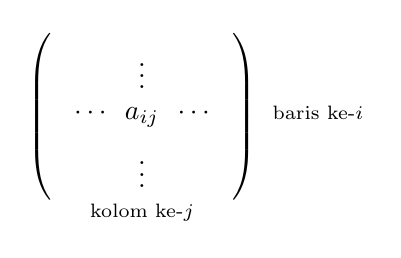
\begin{tikzpicture}[baseline]
			\matrix (M) [matrix of math nodes, left delimiter=(, right delimiter=)] {
				& \vdots & \\
				\cdots & a_{ij} & \cdots \\
				& \vdots & \\
			};
		\node[right=2.5em] at (M-2-3) {\scriptsize baris ke-$i$};
		\node[below=1em] at (M-3-2) {\scriptsize kolom ke-$j$};
	\end{tikzpicture}\]
	dan determinannya ditulis $\det A$. Perkalian matriks $AB=C$ ditentukan oleh $\sum_j a_{ij} b_{jk} = c_{ik}$. Transpos matriks $A$ ditulis ${}^t A$. Matriks identitas $n \times n$ ditulis $1_{n \times n}$ atau $1$.
\end{itemize}

\section*{Struktur aljabar yang umum}
Karena buku ini menitikberatkan interaksi antarkonsep, rujukan silang berskala kecil—atau dengan kata lain ``mendahului pembahasan''—tidak dapat dihindari selama hal itu tidak memengaruhi batang utama teori, terutama pada beberapa bab pertama. Banyaknya manfaat yang diperoleh pembaca bergantung pada pengetahuan yang telah dimiliki. Tabel berikut mencantumkan sejumlah struktur aljabar dasar, baik untuk memudahkan rujukan maupun untuk membantu pembaca menangkap atau mengingat kembali konsep-konsep awal aljabar dengan cepat.

Berikut ini $\GL_n(\R)$ menyatakan himpunan matriks real invertibel berukuran $n \times n$, $M_n(\R)$ menyatakan himpunan matriks real berukuran $n \times n$, dan $\Z/p\Z$ menyatakan sistem kelas residu modulo bilangan prima $p$.
\begin{center}
\scriptsize
\renewcommand{\arraystretch}{1.18}
\begin{tabularx}{\textwidth}{|>{\hsize=.65\hsize}Y|>{\hsize=1.10\hsize}Y|>{\hsize=1.35\hsize}Y|>{\hsize=1.15\hsize}Y|>{\hsize=.75\hsize}Y|} \hline
	\emph{Struktur} & \emph{Operasi} & \emph{Sifat} & \emph{Sifat homomorfisme $\phi$} & \emph{Contoh dasar} \\ \hline
	Himpunan $X$ & Tidak ada & Tidak ada & Pemetaan $X \xrightarrow{\phi} Y$ & $\{1,2,3, \ldots\}$ \\ \hline
	Monoid $M$ & Perkalian $(x,y) \mapsto xy$\newline Unsur identitas $1 \in M$ & Asosiativitas $x(yz)=(xy)z$\newline Sifat identitas $1x = x = x1$ & Pemetaan $M_1 \xrightarrow{\phi} M_2$\newline $\phi(xy)=\phi(x)\phi(y)$\newline $\phi(1)=1$ & $(\Z_{\geq 0}, +)$ \\ \hline
	Grup $G$ & Seperti di atas & Seperti di atas, dan $\forall x$ memiliki invers:\newline $xx^{-1} = 1 = x^{-1} x$ & Seperti di atas & $(\Z, +)$\newline $(\GL_n(\R), \cdot)$ \\ \hline
	Gelanggang $R$ & Grup abelian terhadap penjumlahan\newline Identitas penjumlahan $= 0$\newline Monoid terhadap perkalian\newline Identitas perkalian $= 1$ & Distributivitas:\newline $r(s+s') = rs+rs'$\newline $(s+s')r = sr + s'r$ & Homomorfisme terhadap penjumlahan dan perkalian & $(\Z, +, \cdot)$\newline Gelanggang polinom real\newline ($M_n(\R)$, $+$, $\cdot$) \\ \hline
	Medan $F$ & Seperti di atas & Seperti di atas, dan $\forall x \neq 0$ memiliki invers perkalian:\newline $xx^{-1}=1=x^{-1}x$\newline Perkalian komutatif $xy=yx$ & Seperti di atas & $\Q, \R, \CC$\newline $\Z/p\Z$ \\ \hline
	Modul kiri atas $R$: $M$ & Grup abelian terhadap penjumlahan\newline Perkalian skalar $R \times M \to M$ & $r(m + m') = rm + rm'$\newline $(r+r')m = rm + r'm$\newline $r(r'm) = (rr')m$\newline Sifat identitas $1 m = m$ & Homomorfisme terhadap penjumlahan\newline $\phi(rm) = r\phi(m)$ & Ruang vektor di atas suatu medan \\ \hline
\end{tabularx}
\end{center}

Sebagian pustaka tidak mensyaratkan keberadaan identitas perkalian pada gelanggang. Untuk setiap struktur dalam tabel di atas, pemetaan yang disebut homomorfisme memiliki sifat-sifat berikut:
\begin{compactitem}
	\item pemetaan identitas $\identity_X$ merupakan homomorfisme dari $X$ ke dirinya sendiri (disebut endomorfisme),
	\item komposisi homomorfisme tetap merupakan homomorfisme,
	\item komposisi homomorfisme memenuhi asosiativitas $f \circ (g \circ h)=(f \circ g) \circ h$.
\end{compactitem}
Jika sepasang homomorfisme antarstruktur $\begin{tikzcd} X \arrow[yshift=0.5ex, r, "f"] & Y \arrow[yshift=-0.5ex, l, "g"]\end{tikzcd}$ memenuhi $f \circ g = \identity_Y$ dan $g \circ f = \identity_X$, keduanya disebut saling invers. Dalam hal ini, $f$ dan $g$ saling menentukan secara tunggal; kita tulis $g = f^{-1}$ dan $f = g^{-1}$. Homomorfisme yang invertibel disebut isomorfisme. Ingatlah satu asas dasar aljabar: isomorfisme menghubungkan struktur aljabar yang pada hakikatnya sama.

Jika untuk sementara rincian teori himpunan diabaikan, sifat-sifat di atas menunjukkan bahwa untuk setiap jenis struktur dalam tabel, seluruh anggotanya (``objek'') bersama homomorfisme di antaranya (``morfisme'') membentuk contoh awal suatu \emph{kategori}. Kategori grup, grup abelian, dan modul kiri $R$ biasanya masing-masing ditulis $\cate{Grp}$, $\cate{Ab}$, dan $R\dcate{Mod}$; demikian pula untuk yang lain. Untuk objek $X$, $Y$ dalam kategori-kategori ini, semua homomorfisme di antaranya membentuk himpunan $\Hom_{\cate{Grp}}(X,Y)$, $\Hom_{\cate{Ab}}(X,Y)$, dan seterusnya, yang kerap disingkat menjadi $\Hom(X, Y)$. Homomorfisme dari $X$ ke dirinya sendiri disebut endomorfisme; semuanya membentuk monoid terhadap komposisi morfisme, yang ditulis $\End(X)$. Endomorfisme yang invertibel disebut automorfisme; automorfisme-automorfisme tersebut membentuk grup yang ditulis $\Aut(X)$.

Semua operasi pada struktur dalam tabel dibangun di atas himpunan. Untuk struktur-struktur itu dapat dibuktikan bahwa isomorfisme persis merupakan homomorfisme bijektif. Namun, perlu diperhatikan bahwa:
\begin{compactitem}
	\item suatu kategori tidak harus terdiri atas struktur yang dibangun di atas himpunan;
	\item dalam kategori lain yang objeknya berupa struktur berbasis himpunan, homomorfisme bijektif pun belum tentu invertibel. Contoh tandingan bakunya adalah kategori $\cate{Top}$ (objek = ruang topologis Hausdorff, morfisme = pemetaan kontinu). Isomorfisme di dalamnya adalah homeomorfisme ruang topologis, tetapi pemetaan kontinu yang bijektif belum tentu merupakan homeomorfisme.
\end{compactitem}

Dalam mengkaji homomorfisme antarstruktur, kami sering memakai bahasa diagram komutatif: panah menggambarkan homomorfisme, sedangkan komutativitas berarti bahwa komposisi panah di dalam diagram memberikan hasil yang sama melalui setiap lintasan. Contoh dasarnya ialah
\[\begin{tikzcd}
	A \arrow[r, "f"] \arrow[d, "h"'] & B \arrow[ld, "g"] \\
	C &
\end{tikzcd} \; \text{komutatif} \iff g \circ f = h. \]

Tentu saja, kami juga akan mempertimbangkan diagram yang lebih rumit, misalnya
\[\begin{tikzcd}[scale=0.6]
	A \arrow[r] \arrow[rd] & B \arrow[r] \arrow[d] & C \arrow[d] \\
	& D \arrow[r] & E
\end{tikzcd}\]
dan sebagainya; makna komutativitas dapat diperluas dengan cara yang sama. Komutativitas sebuah diagram dapat diperiksa bagian demi bagian. Misalnya, komutativitas diagram di atas dapat direduksi menjadi pemeriksaan subdiagram \begin{tikzcd} \bullet \arrow[r] \arrow[rd] & \bullet \arrow[d] \\ & \bullet \end{tikzcd} dan \begin{tikzcd} \bullet \arrow[r] \arrow[d] & \bullet \arrow[d] \\ \bullet \arrow[r] & \bullet \end{tikzcd}. Prosedur ini sangat berguna bagi diagram yang lebih rumit, misalnya dalam situasi ``tiga dimensi''.

Karena diagram komutatif hanya melibatkan komposisi panah, diagram tersebut berlaku pula dalam kategori umum.

	% Indonesian LaTeX source for book ``Methods in Algebra''
% Copyright 2018  李文威 (Wen-Wei Li).
% Permission is granted to copy, distribute and/or modify this
% document under the terms of the Creative Commons
% Attribution 4.0 International (CC BY 4.0)
% http://creativecommons.org/licenses/by/4.0/

% To be included
\chapter{Teori himpunan}
Konsep dan operasi dasar himpunan merupakan materi matematika sekolah menengah atau mata kuliah dasar di perguruan tinggi. Bab ini bertujuan memperkukuh dan memperbarui landasan tersebut, serta melengkapinya dengan beberapa pengetahuan dasar yang kerap terlewatkan. Pokok bahasannya ialah:
\begin{compactitem}
	\item perumusan eksplisit teori himpunan aksiomatik Zermelo--Fraenkel beserta aksioma pilihan;
	\item teori ordinal dan lemma Zorn; ordinal dan rekursi transfinit jarang dibahas dalam buku teks aljabar umum, sedangkan pembuktian lemma Zorn pun sering kali sangat berputar-putar;
	\item definisi dan operasi dasar bilangan kardinal;
	\item penjelasan mengenai semesta Grothendieck, yang memungkinkan teori kategori digunakan dengan aman.
\end{compactitem}

Karena corak dan keterbatasan ruang buku ini, topik-topik tersebut hanya dapat disinggung secara ringkas. Dalam kebanyakan keadaan, matematikawan tidak perlu berhadapan langsung dengan struktur terdalam teori himpunan; hasil yang diperlukan pun dapat dianggap telah diketahui. Karena itu, pembaca boleh kembali ke bab ini hanya bila diperlukan. Namun, kajian teori kategori yang serius tidak dapat menghindari persoalan himpunan. Di pihak lain, ordinal, kardinal, dan rekursi transfinit merupakan perangkat sehari-hari bagi peneliti logika matematika dan teori himpunan. Banyak buku aljabar sama sekali tidak membahasnya, atau membahasnya dengan cara yang sukar ditembus. Mengingat metode logika---khususnya teori model \cite{Feng17}---belakangan ini makin merambah geometri, teori bilangan, dan bidang lain, pemahaman atas materi ini tentu bermanfaat. \index{teori model@teori model (model theory)}

\begin{wenxintishi}
	Pembaca harus memiliki pengetahuan paling dasar tentang teori himpunan naif. Semesta Grothendieck hanya diperlukan ketika topik yang lebih lanjut menuntut operasi tingkat tinggi pada kategori. Pembaca yang baru mulai mempelajari aljabar disarankan untuk melewati bab ini untuk sementara.
\end{wenxintishi}

\section{Ikhtisar aksioma ZFC}\label{sec:ZFC}
Apakah himpunan itu? Pada tahun 1895, G.\ Cantor memberikan penjelasan berikut \cite[p.481]{Cantor95}: ``Yang dimaksud dengan himpunan ialah suatu keseluruhan yang terbentuk dengan menghimpun sejumlah objek tertentu dan saling berbeda yang terdapat dalam persepsi atau pikiran kita; objek-objek tersebut disebut anggota himpunan itu.'' Lebih dari seabad kemudian, rumusan Cantor masih harus diakui cermat dan tepat. Meskipun demikian, memanipulasi objek-objek yang ``tertentu'' dan ``saling berbeda'' itu tanpa batas akan menimbulkan paradoks. Paradoks Russell yang termasyhur, misalnya, mempertimbangkan ``himpunan'' $\textbf{V}$ dari semua himpunan, lalu membentuk ``subhimpunan'' $\{x \in \textbf{V} : x \notin x\}$ dan memperoleh kontradiksi.\index{paradoks Russell@paradoks Russell} Pendekatan utama teori himpunan modern ialah membatasi ruang penerapan prinsip komprehensi $\left\{x : x \text{ memenuhi sifat } P\right \}$, lalu melakukan deduksi dalam logika orde pertama dengan sistem aksioma yang sesuai. Sebagai contoh, ``himpunan'' $\textbf{V}$ di atas sebenarnya bukan himpunan; paling jauh ia dapat disebut kelas.\index{teori himpunan@teori himpunan}

Buku ini menggunakan teori himpunan aksiomatik Zermelo--Fraenkel yang lazim dan menerima aksioma pilihan; sistem ini disingkat ZFC.\index{teori himpunan!ZFC} Kelak kita akan menambahkan satu aksioma mengenai kardinal besar (Hipotesis \ref{hyp:universe}). Secara sangat garis besar, ZFC dibangun di atas:
\begin{itemize}
	\item logika orde pertama, yang memuat konektif logis dan kuantor seperti $\wedge$, $\neg$, $\implies$, $\forall$, dan $\exists$, tanda kurung $(\;)$, variabel $x, y, z, \ldots$, tanda sama dengan $=$ (dipandang sebagai predikat biner), dan sebagainya; dapat ditentukan apakah suatu formula mengikuti kaidah bahasa itu---misalnya, apakah tanda kurungnya berpasangan dengan benar---dan formula yang memenuhi kaidah disebut formula terbentuk baik. Bahasa ini merupakan landasan baku logika formal; lihat \cite[Bab 2]{Feng17}.
	\item predikat biner $\in$ yang diperlukan teori himpunan, beserta aksioma \textbf{A.1} --- \textbf{A.9} yang akan dicantumkan di bawah. Jika $x \in y$, maka $x$ disebut anggota $y$. Semua objek $x,y$, dan seterusnya yang ditangani ZFC harus dipahami sebagai himpunan. Secara khusus, anggota suatu himpunan juga merupakan himpunan, sedangkan himpunan $s$ dan himpunan tunggal (\emph{singleton}) yang hanya beranggotakan $s$, yakni $\{s\}$, adalah dua hal yang berbeda.
\end{itemize}

Pada tataran logika, buku ini mengandalkan pemahaman umum. Kita tidak memakai formalisme ketat logika orde pertama, tetapi hanya menguraikan aksioma ZFC dalam bahasa informal yang digunakan matematikawan sehari-hari; seluruh deduksi formal selanjutnya dihilangkan. Rinciannya dapat ditemukan dalam buku teori himpunan mana pun, misalnya \cite{Je03,HY14}; untuk ikhtisar ringkas, lihat \cite{sep-set-theory}.
\begin{enumerate}[\bfseries {A}.1]
	\item \emph{Aksioma ekstensionalitas}: jika dua himpunan mempunyai anggota yang sama, maka kedua himpunan itu sama.

		Definisi formal himpunan kosong $\emptyset$ ialah $\{u \in X: u \neq u\}$, dengan $X$ suatu himpunan sembarang. Salah satu penerapan aksioma ekstensionalitas yang nyaris sepele ialah membuktikan bahwa $\emptyset$ tidak bergantung pada pilihan $X$, asalkan suatu himpunan memang ada. Syarat keberadaan ini dapat dijadikan ``aksioma eksistensi'' tersendiri atau dimasukkan ke dalam aksioma ketakhinggaan di bawah.
	\item \emph{Aksioma pasangan}: untuk setiap $x,y$, terdapat himpunan $\{x,y\}$ yang anggotanya tepat $x$ dan $y$.
	
		Konsep pasangan berurutan $(x,y)$ dapat direalisasikan dengan aksioma pasangan: kita dapat mendefinisikan $(x,y) := \{\{x\}, \{x,y\} \}$, lalu mendefinisikan hasil kali Kartesius $X \times Y := \{(x,y) : x \in X,\; y \in Y \}$; dengan cara yang sama dapat didefinisikan hasil kali sejumlah berhingga himpunan $X \times Y \times \cdots$. Suatu pemetaan antarahimpunan $f: X \to Y$ diidentifikasi dengan grafnya $\Gamma_f \subset X \times Y$: untuk setiap $x \in X$, irisan $\Gamma_f \cap (\{x\} \times Y)$ merupakan himpunan tunggal, yang ditulis $\{(x, f(x))\}$.
	\item \emph{Skema aksioma pemisahan}: misalkan $P$ suatu sifat himpunan, dan $P(u)$ menyatakan bahwa himpunan $u$ memenuhi sifat $P$. Untuk setiap himpunan $X$, terdapat himpunan $Y = \{u \in X : P(u) \}$.
	\item \emph{Aksioma gabungan}: untuk setiap himpunan $X$, terdapat gabungan yang bersesuaian, yaitu $\bigcup X := \{u : \exists v \in X \; \text{ sedemikian sehingga }\; u \in v\}$.
	
		Dalam aksioma ini, $X$ biasanya dipandang sebagai suatu keluarga himpunan; karena itu, $\bigcup X$ juga ditulis sebagai $\bigcup_{v \in X} v$.
	\item \emph{Aksioma himpunan kuasa}: untuk setiap himpunan $X$, seluruh subhimpunannya membentuk suatu himpunan $P(X) := \{u : u \subset X \}$.\index[sym1]{$P(X)$}
	\item \emph{Aksioma ketakhinggaan}: terdapat suatu himpunan tak hingga.

		Apakah yang dimaksud dengan himpunan tak hingga? Karakterisasi sifat ini tidak langsung tampak. Dalam bahasa formal, aksioma ketakhinggaan dapat ditulis sebagai
		\begin{gather}\label{eqn:infinity-axiom}
			\exists x \bigl[ (\emptyset \in x) \;\wedge \;\forall y \in x \left(y \cup \{y\} \in x \right)  \bigr].
		\end{gather}
		Himpunan $x$ semacam ini disebut himpunan induktif. Tujuan mengandaikan keberadaan himpunan induktif ialah mengambil darinya subhimpunan
		\[ \left\{\emptyset, \{\emptyset\}, \{  \emptyset, \{\emptyset\}\}, \{  \emptyset, \{\emptyset\}, \{  \emptyset, \{\emptyset\}\}\}, \ldots \right\}, \]
		yaitu ordinal tak hingga terhitung $\omega$ yang akan segera kita konstruksi.
	\item \emph{Skema aksioma penggantian}: misalkan $F$ suatu fungsi dengan domain berupa himpunan $X$. Maka terdapat himpunan $F(X) = \{ F(x) : x \in X\}$.
	
		Sifat $P$ dan fungsi $F$ dalam skema aksioma pemisahan dan penggantian bukan definisi biasa dalam pengertian teori himpunan, sehingga tidak menimbulkan penalaran melingkar. Keduanya sebenarnya didefinisikan oleh formula terbentuk baik dalam logika orde pertama. Sebagai contoh, fungsi $x \mapsto y$ dapat ditafsirkan sebagai formula terbentuk baik dalam logika orde pertama dengan dua variabel bebas $x,y$, katakanlah $\varphi$, yang memenuhi $\forall x\; \exists! y\; \varphi(x,y)$. Karena setiap pilihan $P$ atau $F$ menghasilkan satu aksioma yang bersesuaian, aksioma pemisahan dan penggantian masing-masing berbentuk skema aksioma.
	\item \emph{Aksioma regularitas}: setiap himpunan tak kosong memuat suatu anggota yang minimal terhadap relasi keanggotaan $\in$.
	
		Salah satu akibat penting aksioma regularitas ialah bahwa, untuk setiap himpunan $x$, tidak ada rantai keanggotaan tak hingga $x \ni x_1 \ni x_2 \ni \cdots$; khususnya, $x \notin x$. Dari sini dapat dibangun hierarki kumulatif himpunan; lihat \S\ref{sec:Grot-universe}.
	\item \emph{Aksioma pilihan}: misalkan setiap anggota himpunan $X$ merupakan himpunan tak kosong. Maka terdapat fungsi $g: X \to \bigcup X$ sedemikian sehingga $\forall x \in X, \; g(x) \in x$ (disebut fungsi pilihan).\index{aksioma pilihan@aksioma pilihan (axiom of choice)}

		Dalam aksioma pilihan, $X$ hendaknya dibayangkan sebagai suatu keluarga himpunan tak kosong. Fungsi pilihan $g(x) \in x$ berarti bahwa satu anggota dipilih dari setiap himpunan $x \in X$.
\end{enumerate}

Secara ketat, sistem formal ZFC hanya membicarakan himpunan. Beberapa teori himpunan aksiomatik yang lazim, seperti sistem NBG (von Neumann--Bernays--Gödel)\index{teori himpunan!NBG}, juga mendefinisikan konsep \emph{kelas}: setiap himpunan merupakan kelas, tetapi terdapat pula kelas yang bukan himpunan, yang disebut \emph{kelas sejati}\index{kelas sejati@kelas sejati (proper class)}. Dalam sistem ZFC, kelas hanyalah alat bantu: pada tingkat metabahasa, kelas dipahami sebagai semua himpunan yang memenuhi suatu sifat tertentu; misalnya, semua himpunan membentuk suatu kelas. Operasi pada kelas direduksi menjadi operasi pada formula terbentuk baik dalam logika orde pertama. Buku ini berusaha menghindari kelas sejati, tetapi dalam bab ini kita tetap harus menanganinya.

Gabungan $X \cup Y$, irisan $X \cap Y$, selisih $X \smallsetminus Y$, hasil kali $X \times Y$, relasi subhimpunan $X \subset Y$, fungsi, dan sebagainya merupakan konsep-konsep turunan. Pembaca tentu telah sangat mengenalnya, sehingga tidak akan diuraikan lagi. Dari konsep-konsep ini selanjutnya dapat dikonstruksi himpunan bilangan bulat taknegatif $\Z_{\geq 0}$, himpunan bilangan bulat $\Z$, himpunan bilangan rasional $\Q$, himpunan bilangan real $\R$, dan seterusnya. Dalam \S\ref{sec:order}, kita akan meninjau kembali cara mengonstruksi $\Z_{\geq 0}$ dalam teori himpunan.

Berikut ini kita uraikan secara ringkas konsep himpunan hasil bagi. Untuk setiap $n \geq 1$, pada himpunan $X$, relasi $n$-er didefinisikan sebagai suatu subhimpunan dari $X^n = \underbracket{X \times \cdots \times X}_{n\; \text{faktor}}$, yang dinyatakan dengan $R$. Dalam kebanyakan keadaan, yang dipertimbangkan ialah relasi biner; dalam hal ini, $xRy$ menyatakan $(x,y) \in R$. Suatu relasi biner $\sim$ yang memenuhi sifat-sifat berikut disebut \emph{relasi ekuivalensi}:
\begin{compactdesc}
	\item[Refleksif] $x \sim x$,
	\item[Simetris] $x \sim y \implies y \sim x$,
	\item[Transitif] $(x \sim y) \wedge (y \sim z) \implies (x \sim z)$.
\end{compactdesc}
Untuk $X$ dengan relasi ekuivalensi $\sim$ dan setiap $x \in X$, kelas ekuivalensi yang memuat $x$ ditulis $[x] := \{y \in X: y \sim x \}$. \emph{Himpunan hasil bagi}\index{himpunan hasil bagi@himpunan hasil bagi (quotient)} didefinisikan sebagai himpunan seluruh kelas ekuivalensi, yaitu $X/\sim\; := \{[x] : x \in X \}$. Dengan demikian diperoleh dekomposisi $X$ sebagai gabungan saling lepas (juga disebut partisi $X$), yakni $X = \bigcup_{[x] \in X/\sim} [x]$. Selain itu, $x \sim y$ jika dan hanya jika $x,y$ termasuk dalam subhimpunan yang sama pada partisi tersebut. Mudah dilihat bahwa relasi ekuivalensi pada $X$ berkorespondensi satu-satu dengan partisi $X$.

Kita akan menggunakan notasi teori himpunan yang lazim. Misalnya, $X \subsetneq Y$ berarti $X \subset Y$ dan $X \neq Y$; $X \sqcup Y$ menyatakan gabungan saling lepas $X$ dan $Y$; sedangkan $X^Y$ \index[sym1]{$X^Y$} menyatakan himpunan semua fungsi $f: Y \to X$. Khususnya, $2^X = P(X)$\index[sym1]{$2^X$}, dengan $2$ menyatakan suatu himpunan yang mempunyai tepat dua anggota. Kita akan menggunakan $\{\text{pt}\}$ untuk menyatakan himpunan yang mempunyai tepat satu anggota. Selanjutnya, untuk suatu himpunan indeks $I$ dan suatu keluarga himpunan $(X_i)_{i \in I}$, dapat didefinisikan
\[ \begin{array}{ll}
	\text{gabungan } \; \bigcup_{i \in I} X_i, & \text{irisan } \; \bigcap_{i \in I} X_i, \quad (I \neq \emptyset), \\
	\text{gabungan saling lepas } \; \bigsqcup_{i \in I} X_i, & \text{hasil kali } \; \prod_{i \in I} X_i.
\end{array}\]
Untuk $I=\emptyset$, gabungan dan gabungan saling lepas keduanya adalah $\emptyset$, sedangkan hasil kalinya adalah $\{\emptyset\}$. Satu-satunya definisi yang wajar bagi irisan kosong ialah kelas $\textbf{V}$ yang terdiri atas semua himpunan, tetapi hal ini tidak diperbolehkan dalam sistem ZFC.

Teori himpunan aksiomatik merupakan landasan ortodoks matematika modern. Cakupan pengungkapannya begitu luas dan taraf formalisasinya begitu tinggi sehingga matematika itu sendiri dapat menjadi objek penelitian matematika. Pertanyaan seperti apakah yang dimaksud dengan bukti, apakah suatu pernyataan dapat dibuktikan, dan apakah suatu sistem aksioma konsisten (bebas kontradiksi), semuanya dapat diberi kandungan matematis yang jelas; bidang penelitian semacam ini secara kolektif disebut metamatematika\index{metamatematika@metamatematika (metamathematics)}. Definisi, argumen, dan praktik matematika lain yang biasanya disampaikan dalam bahasa alami ``pada prinsipnya'' dapat ditulis ulang dalam bahasa formal ZFC atau teori himpunan aksiomatik lainnya, sehingga perumusan dan verifikasinya memperoleh landasan yang kukuh. Entah itu suatu keberuntungan atau kemalangan, selama ini landasan tersebut tak lebih daripada suatu sikap pada tataran prinsip: bahkan perumusan formal teorema teori himpunan yang tampak sederhana pun sering sangat bertele-tele, apalagi jika harus diverifikasi atau bahkan dipahami secara manual. Namun, seiring kemajuan berkelanjutan dalam logika simbolik, teori komputasi, dan teknologi terkait, keadaan ini berangsur-angsur berubah. Hasil-hasil seperti teorema empat warna, teorema bilangan prima, dan dugaan Kepler kini telah memiliki verifikasi formal, dan penerapan metode formal tidak terbatas pada matematika. Gagasan-gagasan di luar teori himpunan, seperti teori tipe, tampaknya diperlukan untuk tujuan ini, atau setidaknya memberikan penyederhanaan yang sangat besar. Satu hal dapat dipastikan: seiring teori dan teknologi berkembang bersama, pemahaman manusia mengenai landasan maupun praktik matematika akan terus ditulis ulang.
\ifdefined\UnitTwoZFCReader\expandafter\endinput\fi
\section{Struktur Urutan dan Ordinal}\label{sec:order}
Menurut pandangan Bourbaki, struktur urutan, bersama struktur topologis dan struktur aljabar, membentuk tiga struktur induk utama matematika. Berikut ini diperkenalkan secara berurutan konsep urutan parsial, urutan total, dan urutan baik.

\begin{definition}\label{def:partial-order}\index{himpunan terurut parsial@himpunan terurut parsial (partially ordered set/poset)}\index{himpunan praterurut@himpunan praterurut (pre-ordered set)}
	Suatu \emph{himpunan terurut parsial} (atau \emph{poset}) adalah data $(P, \leq)$, dengan $P$ suatu himpunan dan $\leq$ suatu relasi biner pada $P$ (urutan parsial), yang memenuhi
	\begin{compactdesc}
		\item[Refleksivitas] $\forall x \in P, \; x \leq x$;
		\item[Transitivitas] $(x \leq y) \wedge (y \leq z) \implies x \leq z$;
		\item[Antisimetri] $(x \leq y) \wedge (y \leq x) \implies x=y$.
	\end{compactdesc}
	Struktur dengan refleksivitas dan transitivitas saja disebut \emph{himpunan praterurut}. Untuk himpunan praterurut, peta yang memenuhi $x \leq y \implies f(x) \leq f(y)$ disebut \emph{peta pelestari urutan}.

	Pada umumnya, $x < y$ digunakan untuk menyatakan $x \leq y$ dan $x \neq y$. Makna simbol $\geq$ dan $>$ jelas dengan sendirinya. Selanjutnya, ketika membicarakan himpunan terurut parsial, relasi $\leq$ di dalamnya sering dihilangkan dari notasi.
\end{definition}

Misalkan $P, Q$ himpunan terurut parsial. Jika peta $\phi: P \to Q$ memenuhi $(x < x') \implies (\phi(x) < \phi(x'))$, maka $\phi$ disebut naik tegas. Jika $\phi: P \to Q$ merupakan bijeksi dan $\phi, \phi^{-1}$ keduanya merupakan peta pelestari urutan, maka $\phi$ disebut isomorfisme antara himpunan terurut parsial $P,Q$. Kelas isomorfisme dari suatu himpunan terurut parsial disebut \emph{tipe urutan}. Setiap subhimpunan dari himpunan terurut parsial mewarisi struktur urutan parsial yang alami.

\begin{definition}\label{def:max-sup}\index{elemen maksimal@elemen maksimal (maximal element)}\index{batas atas@batas atas (upper bound), supremum}\index{batas bawah@batas bawah (lower bound), infimum}
	Misalkan $P' \subset P$, dengan $P$ suatu himpunan praterurut.
	\begin{compactitem}
		\item Elemen $x \in P$ disebut elemen maksimal dari $P$ jika tidak terdapat $y \in P$ yang memenuhi $x < y$;
		\item Elemen $x \in P$ disebut batas atas dari $P'$ jika $x' \leq x$ untuk setiap $x' \in P'$;
		\item Elemen $x \in P$ disebut supremum dari $P'$ jika $x$ merupakan batas atasnya dan $x \leq y$ untuk setiap batas atas $y$.
	\end{compactitem}
	Dengan cara serupa dapat didefinisikan elemen minimal, batas bawah, dan infimum, cukup dengan mengganti $\leq$ di atas dengan $\geq$. Untuk himpunan terurut parsial $P$, antisimetri memastikan bahwa supremum atau infimum suatu subhimpunan $P'$, jika ada, bersifat unik; masing-masing dinotasikan dengan $\sup P'$ dan $\inf P'$. \index[sym1]{sup@$\sup$}\index[sym1]{inf@$\inf$}
\end{definition}

\begin{definition}\label{def:filtrant-poset}\index{poset terarah ke atas@poset terarah ke atas (filtered poset)}
	Jika himpunan terurut parsial $P$ tidak kosong dan, untuk setiap $x,y \in P$, subhimpunan $\{x,y\}$ mempunyai batas atas, maka $P$ disebut \emph{poset terarah ke atas} (\emph{filtered poset}).
\end{definition}

\begin{definition}\index{himpunan terurut total@himpunan terurut total (totally ordered set)}\index{rantai@rantai (chain)}
	Jika setiap pasangan elemen $x,y$ dalam himpunan terurut parsial $P$ dapat dibandingkan (yakni, $x \leq y$ atau $y \leq x$), maka $P$ disebut \emph{himpunan terurut total}. Himpunan terurut total juga disebut \emph{himpunan terurut linear} atau \emph{rantai}.
\end{definition}
Jelas bahwa setiap himpunan terurut total terarah ke atas.

Sesekali kita juga akan membicarakan urutan atau urutan total pada kelas tertentu, beserta batas atas, batas bawah, dan sebagainya; contohnya ialah kelas ordinal $\textbf{On}$ yang akan dibahas di bawah. Definisinya sama seperti di atas.

\begin{definition}[G.\ Cantor]\label{def:well-ordered}\index{himpunan terurut baik@himpunan terurut baik (well-ordered set)}
	Himpunan terurut total $P$ disebut \emph{himpunan terurut baik} jika memenuhi sifat berikut: setiap subhimpunan tak kosong dari $P$ mempunyai elemen minimal.
\end{definition}

\begin{example}
	Untuk sebarang himpunan $X$, himpunan kuasa $P(X)$, terhadap relasi inklusi $\subset$, merupakan poset terarah ke atas, tetapi pada umumnya tidak terurut total. Himpunan bilangan bulat taknegatif $\Z_{\geq 0}$ dan himpunan bilangan real $\R$, yang akan dikonstruksi kemudian, keduanya mempunyai struktur urutan total baku; di antaranya, $\Z_{\geq 0}$ jelas terurut baik, sedangkan $\R$ tidak.
\end{example}

\begin{lemma}\label{prop:wellorder-automorphism}
	Misalkan $P$ himpunan terurut baik dan peta $\phi: P \to P$ naik tegas. Maka $\phi(x) \geq x$ untuk setiap $x \in P$. Khususnya:
	\begin{inparaenum}[(i)]
		\item $P$ tidak mempunyai automorfisme taktrivial,
		\item untuk setiap $x \in P$, tidak terdapat isomorfisme dari $P$ ke $P_{< x} := \{y \in P : y < x \}$.
	\end{inparaenum}
\end{lemma}
Subhimpunan berbentuk $P_{< x}$ mewarisi urutan baik dari $P$ dan disebut sebuah \emph{segmen awal} dari $P$.
\begin{proof}
	Andaikan himpunan $P_0 := \{x \in P : \phi(x) < x \}$ tidak kosong. Untuk setiap $z \in P_0$, karena $\phi$ naik tegas, diperoleh $\phi(\phi(z)) < \phi(z)$. Mengambil $z$ sebagai elemen minimal dari $P_0$ menghasilkan kontradiksi. Pernyataan pertama pun terbukti.

	Untuk (i), terapkan pernyataan pertama kepada $\phi$ dan $\phi^{-1}$ sehingga diperoleh $\forall x \; \phi(x)=x$. Untuk (ii), suatu isomorfisme $\phi: P \to P_{< x}$ tentu merupakan peta naik tegas dari $P$ ke dirinya sendiri dan memenuhi $\phi(x) < x$, bertentangan dengan hasil sebelumnya.
\end{proof}

Gagasan awal mengenai ordinal ialah tipe urutan dari suatu himpunan terurut baik. Jika pendekatan ini diikuti, tipe urutan tersebut harus dipandang sebagai kelas, bukan himpunan. Dengan demikian, membicarakan kelas semua ordinal $\textbf{On}$ sama dengan menangani ``kelas dari kelas'', yang jelas agak rumit. Untungnya, dari setiap tipe urutan baik kita dapat memilih sebuah himpunan terurut baik yang baku sehingga memperoleh deskripsi yang lebih tepat. Untuk itu diperlukan definisi von Neumann berikut.
\begin{definition}\label{def:ordinal}\index{ordinal@ordinal}
	Jika setiap elemen suatu himpunan $\alpha$ merupakan subhimpunan dari $\alpha$ (dengan kata lain, $\alpha \subset P(\alpha)$), maka $\alpha$ disebut \emph{transitif}. Jika relasi $x < y \stackrel{\text{def}}{\iff} x \in y$ memberikan urutan baik pada himpunan transitif $\alpha$, maka $\alpha$ disebut \emph{ordinal}.
\end{definition}

Jelas bahwa $\emptyset$ merupakan ordinal. Jika $\alpha$ merupakan ordinal, maka $\alpha \sqcup \{\alpha\}$ juga demikian. Teori lengkap ordinal dapat ditemukan dalam \cite[\S 2]{Je03} atau \cite[Bab 4]{HY14}; berikut ini hanya dirangkum beberapa sifat penting. Hubungan antara ordinal dan tipe urutan baik diberikan dalam Proposisi \ref{prop:ordinal-ordertype}.

\begin{lemma}\label{prop:ordinal-property}
	Ordinal memenuhi sifat-sifat berikut.
	\begin{compactenum}[(i)]
		\item Jika $\alpha$ merupakan ordinal dan $\beta \in \alpha$, maka $\beta$ juga merupakan ordinal.
		\item Bagi setiap pasangan ordinal $\alpha, \beta$, jika $\alpha \subsetneq \beta$, maka $\alpha \in \beta$.
		\item Bagi setiap pasangan ordinal $\alpha, \beta$, berlaku $\alpha \subset \beta$ atau $\beta \subset \alpha$.
	\end{compactenum}
\end{lemma}
\begin{proof}
	Pertama, kita buktikan (i). Dari transitivitas $\alpha$ diperoleh $\beta \subset \alpha$, dan $(\beta, \in)$ juga merupakan himpunan terurut baik. Selanjutnya, kita buktikan bahwa $\beta$ transitif: misalkan $\tau \in \beta \subset \alpha$; cukup dibuktikan bahwa $x \in \tau \implies x \in \beta$. Karena $\in$ memberikan struktur urutan pada $\alpha$, dari $x \in \tau \in \beta$ diperoleh $x \in \beta$.

	Untuk (ii), tuliskan $<$ bagi $\in$ dan ambil $\gamma$ sebagai elemen minimal dari $(\beta \smallsetminus \alpha, <)$. Kita akan menunjukkan bahwa $\alpha = \{x \in \beta : x < \gamma \}$, sedangkan himpunan di ruas kanan tidak lain adalah $\gamma$. Inklusi $\supset$ mengikuti minimalitas elemen tersebut. Untuk inklusi $\subset$, ambil $y \in \alpha \subset \beta$. Pertama, $\gamma = y$ tidak mungkin; selanjutnya, dari transitivitas $\alpha$ diperoleh $y \subset \alpha$, sehingga kemungkinan $\gamma < y$ juga tersingkir. Jadi $y < \gamma$.

	Untuk (iii), jelas bahwa $\gamma := \alpha \cap \beta$ juga merupakan ordinal. Kita akan menunjukkan bahwa $\gamma = \alpha$ atau $\gamma = \beta$ harus berlaku. Jika tidak, hasil di atas memberikan $\gamma \in \alpha$ dan $\gamma \in \beta$, sehingga $\gamma \in \gamma$; dengan kata lain, $\gamma < \gamma$ dalam himpunan terurut parsial $(\alpha, \leq)$. Ini bertentangan dengan makna $<$, yakni $\leq$ tetapi $\neq$.
\end{proof}

Lemma tersebut langsung memberikan akibat berikut.
\begin{theorem}\label{prop:On-wellorder}
	Definisikan $\textbf{On}$ sebagai kelas yang terdiri atas semua ordinal. \index[sym1]{$\textbf{On}$}
	\begin{compactitem}
		\item Untuk ordinal, definisikan $\beta < \alpha$ jika dan hanya jika $\beta \in \alpha$. Relasi ini memberikan urutan total pada $\textbf{On}$, dan untuk setiap ordinal $\alpha$ berlaku $\alpha = \{ \beta : \beta < \alpha \}$.
		\item Jika $C$ merupakan kelas yang terdiri atas ordinal dan $C \neq \emptyset$, maka $\inf C := \bigcap C$ juga merupakan ordinal, dan $\inf C \in C$; selain itu, $\alpha \sqcup \{\alpha\} = \inf\{ \beta: \beta > \alpha \}$.
		\item Jika $S$ merupakan himpunan yang terdiri atas ordinal dan $S \neq \emptyset$, maka $\sup S := \bigcup S$ juga merupakan ordinal.
	\end{compactitem}
\end{theorem}
Dari sini, $\beta < \alpha$ menyiratkan bahwa $\beta$ merupakan segmen awal dari $\alpha$. Sifat $\alpha = \{\beta: \beta < \alpha \}$ adalah kunci untuk memahami konstruksi ordinal.

Untuk suatu ordinal $\alpha$, tetapkan $\alpha + 1 := \alpha \sqcup \{\alpha\} > \alpha$, yang disebut \emph{penerus} $\alpha$; ini merupakan ordinal terkecil yang lebih besar daripada $\alpha$. Jika $\alpha$ bukan penerus dari ordinal mana pun, mudah dilihat bahwa $\alpha = \sup\{\beta: \beta < \alpha\}$. Ordinal $\alpha$ seperti ini disebut \emph{ordinal limit}\index{ordinal!ordinal limit (limit ordinal)}. Dengan konvensi bahwa $\sup$ dari himpunan kosong bernilai $\emptyset$, ``ordinal nol'' $\emptyset$ merupakan ordinal limit.

\begin{proposition}\label{prop:Ord-class}
	Kelas ordinal $\textbf{On}$ merupakan kelas sejati.
\end{proposition}
\begin{proof}
	Hasil sebelumnya menunjukkan bahwa jika $\textbf{On}$ merupakan himpunan, maka $\sup(\textbf{On})$ terdefinisi, dan ordinal $\sup(\textbf{On}) + 1$ akan lebih besar daripada setiap ordinal, termasuk dirinya sendiri!
\end{proof}
Hal ini disebut paradoks Burali--Forti (1897)\index{paradoks Burali--Forti@paradoks Burali--Forti}; paradoks tersebut muncul lebih dahulu daripada paradoks Russell (1902), meskipun pengaruh paradoks yang terakhir lebih besar.

\begin{example}[Konstruksi ordinal tak hingga $\omega$] \index[sym1]{omega@$\omega$}\leavevmode\par
	Tinjau ordinal $0 := \emptyset$. Dengan mengambil penerus berulang kali, diperoleh ordinal
	\[ 1 := 0 + 1, \quad 2 := 1+1, \quad 3=2+1, \ldots \]
	dan seterusnya. Sekarang kita hendak mendefinisikan ordinal limit tak nol terkecil $\omega$. Jika ordinal seperti itu ada, ia harus memuat semua $0,1,2, \ldots$, dan sesungguhnya ordinal-ordinal itulah seluruh anggotanya. Langkah pertama ialah membuktikan keberadaan ordinal limit tak nol. Ingat kembali konsep himpunan induktif dalam aksioma ketakhinggaan \textbf{A.6}. Jika $x$ merupakan himpunan induktif, ambil $\alpha := \{y \in x : y \subset x, \; y \in \textbf{On} \}$. Langsung dari definisi dapat diverifikasi sifat-sifat berikut:
	\begin{inparaenum}[(a)]
		\item $\emptyset \in \alpha$, sehingga $\alpha$ tidak kosong,
		\item $\alpha$ merupakan ordinal,
		\item $y \in \alpha \implies y + 1 \in \alpha$, sehingga $\alpha$ memang merupakan ordinal limit.
	\end{inparaenum}
	Ambil ordinal $\omega := \inf\{ \text{ordinal limit tak nol} \}$. Inilah ordinal yang dicari. Ordinal $n$ yang memenuhi $n < \omega$ disebut \emph{ordinal berhingga}.

	Hingga isomorfisme, ordinal $\omega = \{n : n=0, 1, \ldots \}$ tidak lain ialah himpunan terurut baik $\Z_{\geq 0}$ yang kita kenal secara intuitif. Konstruksi ini juga dapat dipandang sebagai cara mendefinisikan himpunan bilangan bulat taknegatif dengan bertolak dari himpunan kosong dalam kerangka ZFC. Lebih tepatnya, $\omega$, bersama operasi penerus pada elemen-elemennya $n \mapsto n+1$, memenuhi aksioma aritmetika Peano (lihat \cite[Bab 0, \S 2]{DN00}); itulah seluruh sifat yang kita perlukan untuk bekerja dengan bilangan bulat dalam praktik. Teorema \ref{prop:transfinite-induction} akan membahas salah satu sifat kunci tersebut: induksi matematika.
\end{example}

\section{超穷递归及其应用}
定理 \ref{prop:On-wellorder} 表明真类 $\textbf{On}$ 对 $\leq$ 也有良序性质: 任何由序数构成的类都有极小元. 这立即导向以下结果.
\begin{theorem}[超穷归纳法]\label{prop:transfinite-induction} \index{chaoqiongguinafa@超穷归纳法 (transfinite induction)}
	令 $C$ 为一个由序数构成的类. 假设
	\begin{compactenum}[(i)]
		\item $0 \in C$,
		\item $\alpha \in C \implies \alpha+1 \in C$,
		\item 设 $\alpha$ 为极限序数, 若对每个 $\beta < \alpha$ 皆有 $\beta \in C$, 则 $\alpha \in C$,
	\end{compactenum}
	那么 $C = \textbf{On}$. 如果仅考虑小于某 $\theta$ 的序数而非 $\textbf{On}$ 整体, 断言依然成立.
\end{theorem}
\begin{proof}
	设若不然, 取不在 $C$  中的最小序数 $\alpha \neq 0$, 无论它是后继或极限序数都导致矛盾.
\end{proof}
\begin{remark}
	回忆到 $\theta = \{\alpha \in \textbf{On}: \alpha < \theta \}$. 如取 $\theta = \omega$ 则得到经典的数学归纳法, 此时不涉及情况 (iii).
\end{remark}

定理 \ref{prop:transfinite-induction} 常用以递归地构造一列以序数枚举的数学对象, 它基于某规则 $G$ 如下:
\begin{compactdesc}
	\item[第零项] $a_0 = G(0)$ 给定,
	\item[后继项] 设 $\alpha = \beta+1$, 已知 $a_\beta$, 则可以确定 $a_\alpha = a_{\beta + 1} = G(a_\beta)$,
	\item[极限项] 设 $\alpha$ 是极限序数, 已知 $\{a_\beta : \beta < \alpha \}$, 则可以确定 $a_\alpha = G(\{a_\beta : \beta < \alpha \})$.
\end{compactdesc}
不难想象这将唯一确定一列集合 $a_\alpha$, 兹改述并证明如下. 考虑函数 $G: \textbf{V} \to \textbf{V}$, 虽然 $\textbf{V}$ 是真类, 然而如早先所述, $G$ 可以诠释为一阶逻辑中的某类公式而不影响以下操作. 引入 $\theta$-列的概念: 这是指函数 $a: \theta \to \textbf{V}$, 亦可理解为形如 $\{a_\alpha : \alpha < \theta \}$ 的列.

\begin{theorem}[超穷递归原理]
	对任意序数 $\theta$, 存在唯一的 $\theta$-列 $a$ 使得 $\alpha < \theta \implies a(\alpha) = G(a|_\alpha)$. 特别地, 存在唯一的函数 $a: \textbf{On} \to \textbf{V}$ 使得对每个序数 $\alpha$ 皆有 $a(\alpha) = G(a|_\alpha)$.
\end{theorem}
几点说明:
\begin{inparaenum}[(a)]
	\item 替换公理模式 \textbf{A.7} 确保函数限制 $a|_\alpha$ 可以按寻常方法等同于集合 $\{ (\beta, a(\beta)) : \beta \in \alpha \}$, 故 $G$ 对之可以取值;
	\item 我们将函数限制 $a|_0$ 理解为空集 $0$, 故按定义 $a(0) = G(0)$;
	\item 定理前半段只要求 $G$ 对形如 $\alpha \to \textbf{V}$ 的函数有定义, 其中 $\alpha < \theta$.
\end{inparaenum}
\begin{proof}
	第一步, 若 $\theta$-列 $a, a'$ 皆满足所示性质, 我们断言 $\alpha < \theta$ 蕴涵 $a(\alpha) = a'(\alpha)$, 如是则 $a=a'$: 这对 $\alpha=0$ 已知; 设若这对所有 $\beta < \alpha$ 成立, 那么 $a|_\alpha = a'|_\alpha$ 故 $a(\alpha) = a'(\alpha)$; 应用定理 \ref{prop:transfinite-induction} 遂得以上断言.
	
	第二步是 $\theta$-列 $a$ 的存在性. 当 $\theta=0$ 时为显然. 今设 $\theta > 0$, 并且对任意 $\xi < \theta$, 所求 $\xi$-列 $a[\xi]$ 皆存在, 则由替换公理模式知 $a[\xi]$ 确实是集合间的映射; 由第一步可将诸 $a[\xi]$ 拼接为定义在 $\theta$ 上的函数 $a$ 使得 $a|_\xi = a[\xi]$, 而且使性质 $\alpha < \theta \implies a(\alpha) = G(a|_\alpha)$ 成立, 这是容易的.
	
	最后, 由于 $\textbf{On}$ 无极大元, 根据前两步可以唯一地定义 $a: \textbf{On} \to \textbf{V}$.
\end{proof}

借助超穷递归原理, 能对序数定义类似于非负整数的运算如次. 以下在情形 (iii) 总假设 $\beta$ 是极限序数:
\begin{itemize}
	\item 加法: \begin{inparaenum}[(i)] \item $\alpha + 0 := \alpha$,  \item $\alpha + (\beta + 1) = (\alpha + \beta) + 1$, \item $\alpha + \beta = \sup\{ \alpha + \xi : \xi < \beta\}$. \end{inparaenum}
	\item 乘法: \begin{inparaenum}[(i)] \item $\alpha \cdot 0 := 0$, \item $\alpha \cdot (\beta + 1) = \alpha \cdot \beta + \alpha$, \item $\alpha \cdot \beta = \sup\{\alpha \cdot \xi : \xi < \beta\}$. \end{inparaenum}
	\item 指数: \begin{inparaenum}[(i)] \item $\alpha^0 := 1$, \item $\alpha^{\beta + 1} = \alpha^\beta \cdot \alpha$, \item $\alpha^\beta = \sup\{\alpha^\xi : \xi < \beta\}$. \end{inparaenum}
\end{itemize}
可以验证序数对加法和乘法都满足结合律, 但一般不满足交换律. 施之于 $\alpha, \beta < \omega$ 便得到非负整数上的加法和乘法 (当然这时必须验证交换律). 至此, 我们已经基于公理集合论为 $\Z_{\geq 0}$ 上的算术奠定了基础, 将之加工为 $\Z$ 及 $\Q$ 则可以说是代数学的任务, 手法是大家熟知的. 一般性的工具将在定义--定理 \ref{def:K-group} 和 \S\ref{sec:comm-ring-intro} 予以介绍.

\begin{proposition}\label{prop:ordinal-ordertype}
	对任意良序集 $P$, 存在唯一的序数 $\alpha$ 和良序集之间的同构 $\phi: P \rightiso \alpha$.
\end{proposition}
\begin{proof}
	序数和同构的唯一性源自引理 \ref{prop:wellorder-automorphism} 和引理 \ref{prop:ordinal-property}. 可设 $P \neq \emptyset$, 并选取 $\mho \notin P$ (易见存在性). 以下将以超穷递归定义一族元素 $a_\alpha \in P \sqcup \{\mho\}$, 其中 $\alpha$ 取遍所有序数. 设 $a_0 := \text{min}(P)$, 并递归地定义
	\[ a_\alpha := \begin{cases}
		\text{min}\left( P \smallsetminus \{a_\beta : \beta < \alpha \} \right), & \{a_\beta : \beta < \alpha \} \subsetneq P \\
		\mho, & \{a_\beta : \beta < \alpha \} = P.
	\end{cases}\]
	由于 $P$ 是集合, 必存在最小的序数 $\theta$ 使得 $a_\theta = \mho$, 否则这将蕴涵单射 $a: \textbf{On} \to P$, 分离公理模式 \textbf{A.3} 确保 $a(\textbf{On}) \subset P$ 是集合, 而替换公理模式 \textbf{A.7} 蕴涵 $\textbf{On} = a^{-1}(a(\textbf{On}))$ 亦是集合, 此与命题 \ref{prop:Ord-class} 矛盾. 可验证 $a_\alpha \mapsto \alpha$ 定义了偏序集的同构 $P \to \{\beta : \beta < \theta\} = \theta$.
\end{proof}

以下两个重要结果都依赖于选择公理 \textbf{A.9}. 其中 Zorn 引理是代数学的基本工具之一. 之前的论证技巧还会反复出现.
\begin{theorem}[Zermelo 良序定理, 1904]\label{prop:wellorder-principle}\index{Zermelo 良序定理}
	任意集合 $S$ 都能被赋予良序.
\end{theorem}
\begin{proof}
	我们断言 $S$ 和某个序数 $\theta$ 间存在双射. 选取元素 $\mho \notin S$ 如上. 由选择公理, 可以在 $S$ 的每个非空子集 $S'$ 里拣选元素 $g(S')$. 不妨设 $S$ 非空, 命 $a_0 := g(S)$, 并用超穷递归对每个序数 $\alpha$ 定义
	\[ a_\alpha := \begin{cases}
		g \left( S \smallsetminus \{ a_\beta : \beta < \alpha \} \right), & S \neq \{ a_\beta : \beta < \alpha \} \\
		\mho, & S = \{ a_\beta : \beta < \alpha \}.
	\end{cases}\]
	与先前类似, 因 $S$ 是集合, 故可取极小的 $\theta$ 使得 $a_\theta = \mho$, $S = \{a_\beta: \beta < \theta\}$, 后者和序数 $\theta = \{\beta : \beta < \theta \}$ 之间有显然的双射, 于是导出 $S$ 上的良序.
\end{proof}

\begin{theorem}[Zorn 引理]\label{prop:Zorn}\index{Zorn 引理}
	设 $P$ 为非空偏序集, 而且 $P$ 中每个链都有上界, 则 $P$ 含有极大元.
\end{theorem}
\begin{proof}
	类似于前一个证明. 假定 $P$ 不含极大元. 任取 $a_0 \in P$, 并用超穷递归对每个序数 $\alpha$ 定义 $a_\alpha \in P$, 使得 $\alpha < \beta \Rightarrow a_\alpha < a_\beta$, 其方法如次: 设对每个 $\beta < \alpha$ 都定义了 $a_\beta$ 如上, 则 $(a_\beta)_{\beta < \alpha}$ 在 $P$ 中成一链. 若 $\alpha$ 是极限序数, 则此链必有上界 $a_\alpha \notin \{ a_\beta \}_{\beta < \alpha}$; 若 $\alpha = \gamma + 1$ 是后继序数, 因 $P$ 无极大元故存在 $a_\alpha \in P$ 使得 $a_\alpha > a_\gamma$. 真类 $\textbf{On}$ 据此可以嵌入 $P$, 仿照命题 \ref{prop:ordinal-ordertype} 的论证导出 $\textbf{On}$ 亦是集合, 矛盾.
\end{proof}
已知选择公理, 良序定理和 Zorn 引理相互等价, 任择一者连同 \textbf{A.1} -- \textbf{A.8} 皆给出 ZFC. 本书以选择公理为出发点.

\section{基数}\label{sec:cardinal-number}
基数是描述集合大小的一种标杆, 我们从等势的概念出发, 随后联系到序数.

\begin{definition}\index{dengshi@等势 (equipollence)}
	若两集合 $X, Y$ 之间存在双射 $\phi: X \to Y$, 则称 $X, Y$ \emph{等势}.

	等势构成了集合间的等价关系, 集合 $X$ 的等势类记作 $|X|$. 若存在单射 $\phi: X \to Y$, 则记作 $|X| \leq |Y|$.
\end{definition}

关系 $\leq$ 显然只依赖于等势类, 并满足传递性: $|X| \leq |Y|$, $|Y| \leq |Z|$ 蕴涵 $|X| \leq |Z|$. 我们用 $|X| < |Y|$ 表示 $|X| \leq |Y|$, $|X| \neq |Y|$.  以下证明 $\leq $满足反称性, 因而在等势类上定义了偏序.

\begin{theorem}[Schröder--Bernstein]\label{prop:Schröder-Bernstein}
	若两集合 $X,Y$ 满足 $|X| \leq |Y|$ 和 $|Y| \leq |X|$, 则 $|X|=|Y|$.
\end{theorem}
\begin{proof}
	考虑单射 $f: X \to Y$ 和 $g: Y \to X$. 我们可以在断言中以 $g(Y)$ 代替 $Y$, 从而化约到 $Y \subset X$ 而 $g$ 是包含映射的情形, 即 $f(X) \subset Y \subset X$. 置 $X_0 := X$, $Y_0 := Y$, 我们递归地对所有 $n \in \Z_{\geq 0}$ 定义
	\begin{align*}
		X_{n+1} & := f(X_n), \\
		Y_{n+1} & := f(Y_n).
	\end{align*}
	从而得到一列嵌套的子集
	\[ \underbracket{X_0}_{=X} \supset \underbracket{Y_0}_{=Y} \supset \cdots \supset X_n \supset Y_n \supset X_{n+1} \supset \cdots . \]
	定义映射 $\phi: X \to Y$ 如下
	\[ \phi(x) = \begin{cases}
		f(x), & \text{如果}\; \exists n \geq 0, \; x \in X_n \smallsetminus Y_n, \\
		x, & \text{其他情形}.
	\end{cases} \]
	容易验证 $\phi$ 是良定的双射.
\end{proof}

许多书籍直接将基数定义为等势类. 一如序数的情形, 本章的进路是为每个等势类指定标准的代表元, 从而将基数理解为一类特别的序数. 在此先回顾等势类的基本运算:
\begin{compactenum}[(i)]
	\item $|X|+|Y| = |X \sqcup Y|$,
	\item $|X| \cdot |Y| = |X \times Y|$, 
	\item $|X|^{|Y|} = |X^Y|$.
\end{compactenum}
推而广之, 设 $(X_i)_{i \in I}$ 为以集合 $I$ 为指标的一族集合, 则可定义基数和
\begin{gather}\label{eqn:cardinal-infinite-sum}
	\sum_{i \in I} |X_i| := \left\lvert \bigsqcup_{i \in I} X_i \right\rvert.
\end{gather}
与积
\begin{gather}\label{eqn:cardinal-infinite-prod}
	\prod_{i \in I} |X_i| := \left\lvert \prod_{i \in I} X_i \right\rvert.
\end{gather}
可验证两者都是良定的运算. 关于基数之无穷和与无穷积的进一步讨论可参阅 \cite[pp.52-55]{Je03}.

另外注意到 $2^{|X|} = |P(X)|$. 下述定理是熟知的.

\begin{theorem}[Cantor]\label{prop:Cantor}
	对任意集合 $X$ 皆有 $|P(X)| > |X|$.
\end{theorem}
\begin{proof}
	存在单射 $X \to P(X)$, 然而任何映射 $\phi: X \to P(X)$ 皆非满: 仅需验证集合 $Y := \{x \in X : x \notin \phi(x) \}$ 不在 $\phi$ 的像里.
\end{proof}

\begin{definition}\index{jishu@基数 (cardinal)}
	序数 $\kappa$ 称为\emph{基数}, 如果对任意序数 $\lambda < \kappa$ 都有 $|\lambda| < |\kappa|$.
\end{definition}
换言之, 基数无非是一个等势类中的极小序数. 现在我们用选择公理联系等势类和基数.

\begin{proposition}
	对任意集合 $X$, 可取最小的序数 $\alpha(X)$ 使得 $|X|=|\alpha(X)|$. 则 $X \mapsto \alpha(X)$ 给出等势类和基数的一一对应. 特别地, 对任意集合 $X, Y$ 必有 $|X| \leq |Y|$ 或 $|Y| \leq |X|$.
\end{proposition}
\begin{proof}
  序数 $\alpha(X)$ 的存在性源于定理 \ref{prop:wellorder-principle}, 它显然是基数. 其余断言是显然的. 
\end{proof}

据此可以谈论一个集合的基数. 不难证明有限序数和 $\omega$ 都是基数. \emph{有限集}是基数为有限序数的集合, \emph{可数集}是基数为 $\omega$ 的集合, 其余称为\emph{不可数集}; 注意到任何无穷集总是包含一份与 $\Z_{\geq 0}$ 等势的子集, 这是因为无穷序数皆包含 $\omega$. 为了符号上方便, 今后我们将经常混同集合的等势类及相应的基数. \index{keshuji@可数集 (countable set)}

\begin{lemma}\label{prop:cardinal-sup}
	对任意序数 $\alpha$ 都存在基数 $\kappa > \alpha$. 如果 $S$ 是一个由基数构成的集合, 则 $\sup S$ 也是基数.
\end{lemma}
\begin{proof}
	一个集合及其子集上所有可能的良序结构形成一个集合, 而 $\textbf{On}$ 是真类, 因此对任意 $X$ 总存在序数 $\theta$ 使得 $|\theta| > |X|$; 取 $X=\alpha$ 便得到第一个断言. 对于第二个断言, 假定存在序数 $\beta < \alpha := \sup S$ 使得 $|\beta| = |\alpha|$. 根据上确界性质, 必存在 $\kappa \in S$ 满足 $\kappa > \beta$, 因此 $|\beta| \leq |\kappa| \leq |\alpha| = |\beta|$, $|\beta|=|\kappa|$, 这与 $\kappa$ 是基数矛盾.
\end{proof}

任意无穷集 $\alpha$ 都满足 $|\alpha \sqcup \{\alpha\}| = |\alpha|$ (处理 $\alpha=\Z_{\geq 0}$ 的情形即可), 所以无穷基数必为极限序数. 无穷基数称作 $\aleph$ 数. 引理 \ref{prop:cardinal-sup} 告诉我们如何用序数枚举无穷基数: 递归地定义\index[sym1]{aleph@$\aleph_\alpha$}
\begin{align*}
	\aleph_0 & := \omega, \quad \text{这是最小的无穷基数}; \\
	\aleph_{\alpha+1} & := \text{大于 $\aleph_\alpha$ 的最小基数}; \\
	\aleph_\alpha & := \sup_{\beta < \alpha} \aleph_\beta, \quad \text{若 $\alpha$ 是极限序数}.
\end{align*}
特别地, 基数全体构成一个真类.

\begin{example}[Cantor]\label{eg:continuum}
	我们证明 $|\R| = 2^{\aleph_0}$. 首先留意到 $|\Q|=|\Z_{\geq 0}|=\aleph_0$. Dedekind 分割 $x \mapsto \{r \in \Q: r < x \}$ 给出 $\R \hookrightarrow P(\Q)$, 于是 $|\R| \leq |P(\Q)|=2^{\aleph_0}$. 另一方面, 区间 $[0,1]$ 包含 Cantor 集
	\[ C := \left\{ \sum_{n=1}^\infty a_n 3^{-n}: \forall n, \; a_n = 0 \;\text{或}\; 2  \right\}, \]
	形式如上的 $3$ 进制表法是唯一的, 因此 $|\R| \geq |C| = 2^{\aleph_0}$. 应用定理 \ref{prop:Schröder-Bernstein} 即得所求.
\end{example}

集合论中常称实数集为``连续统''. 著名的连续统假设断言 $2^{\aleph_0} = \aleph_1$. 已知若预设 ZFC 公理系统的一致性, 那么无论是连续统假设 (P.\ Cohen, 1963) 或其否定 (K.\ Gödel, 1940) 都无法从 ZFC 的公理推出.

\begin{theorem}[$\alpha \times \alpha$ 上的典范良序]\label{prop:Ord2-canonical}
	真类 $\textbf{On}^2 = \textbf{On} \times \textbf{On}$ 上存在良序 $\prec$ 使得对每个序数 $\alpha$ 皆有 $\textbf{On}^2_{\prec (0, \alpha)} = (\alpha \times \alpha, \prec)$, 称作 $\alpha \times \alpha$ 上的典范良序. 进一步, $(\aleph_\alpha \times \aleph_\alpha, \prec)$ 的序型为 $\aleph_\alpha$; 作为推论, $\aleph_\alpha \cdot \aleph_\alpha = \aleph_\alpha$.
\end{theorem}
\begin{proof}
	在 $\textbf{On}^2$ 上定义 $(\alpha, \beta) \prec (\alpha', \beta')$ 当且仅当
	\begin{compactitem}
		\item $\max\{\alpha, \beta\} < \max\{\alpha', \beta'\}$, 或者
		\item $\max\{\alpha, \beta\} = \max\{\alpha', \beta'\}$, 此时以字典序比大小 (即先比较第一个分量, 相等则比第二个分量).
	\end{compactitem}
	易见 $\prec$ 是 $\textbf{On}^2$ 上的良序. 而且 $0$ 是最小序数故 $(\alpha', \beta') \prec (0, \alpha) \iff \alpha', \beta' < \alpha$. 于是 $\textbf{On}^2_{\prec (0, \alpha)} = \alpha \times \alpha$.
	
	如果 $(\aleph_\alpha \times \aleph_\alpha, \prec)$ 的序型为 $\aleph_\alpha$, 那么基数的定义 (一个等势类中的极小序数) 说明 $|\aleph_\alpha \times \aleph_\alpha| = \aleph_\alpha$, 以基数乘法来表示即 $\aleph_\alpha \cdot \aleph_\alpha = \aleph_\alpha$. 下面就来证明关于序型的断言.

	反设 $\alpha$ 为使得 $(\aleph_\alpha \times \aleph_\alpha, \prec)$ 不同构于 $\aleph_\alpha$ 的最小序数. 此处必有 $\alpha > 0$, 因为 $(\aleph_0 \times \aleph_0, \prec) \simeq \aleph_0$ 由下图给出.
	\begin{center}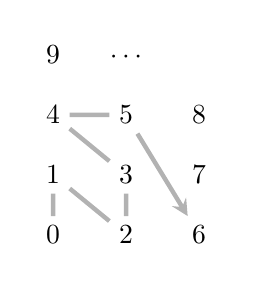
\begin{tikzpicture}
		\matrix (A) [matrix of math nodes, row sep=3mm, column sep=4mm] {
			9 & \cdots & \\
			4 & 5 & 8 \\
			1 & 3 & 7 \\
			0 & 2 & 6 \\
		};
		\draw[ultra thick, -stealth, black!30] (A-4-1) -- (A-3-1) -- (A-4-2) -- (A-3-2) -- (A-2-1) -- (A-2-2) -- (A-4-3);
	\end{tikzpicture} \qquad \begin{tikzpicture}
		\draw[->] (0,0) -- (1.5, 0) node[right] {$\aleph_0$};
		\draw[->] (0,0) -- (0, 1.5) node [above] {$\aleph_0$};
	\end{tikzpicture}\end{center}
	令序数 $\gamma$ 表 $(\aleph_\alpha \times \aleph_\alpha, \prec)$ 之序型, 并取同构 $f: \gamma \rightiso (\aleph_\alpha \times \aleph_\alpha, \prec)$. 基数的性质给出
	\[ \gamma \geq |\gamma| = |\aleph_\alpha \times \aleph_\alpha| \geq \aleph_\alpha; \]
	而 $\alpha$ 的选取蕴涵 $\gamma \neq \aleph_\alpha$, 故 $\gamma > \aleph_\alpha$. 既然 $\aleph_\alpha$ 是 $\gamma$ 的真前段, 限制 $f$ 就得到从 $\aleph_\alpha$ 至 $(\aleph_\alpha \times \aleph_\alpha, \prec)$ 的某个真前段的同构. 根据 $\prec$ 的定义, 存在序数 $\sigma < \aleph_\alpha$ 使得 $f(\aleph_\alpha) \subset \sigma \times \sigma$. 由于 $\aleph_\alpha$ 无穷, $\sigma$ 亦然.
	
	根据基数定义, 存在 $\beta < \alpha$ 使得 $|\sigma| = \aleph_\beta$. 关于 $\alpha$ 的极小性假设蕴涵 $\aleph_\beta \cdot \aleph_\beta = \aleph_\beta$. 但这么一来
	\[ \aleph_\alpha = |f(\aleph_\alpha)| \leq |\sigma| \cdot |\sigma| = \aleph_\beta \cdot \aleph_\beta = \aleph_\beta \]
	遂与 $\beta < \alpha \implies \aleph_\beta < \aleph_\alpha$ 矛盾. 证毕.
\end{proof}

\begin{corollary}\label{prop:cardinal-max}
	对任意非零基数 $\kappa$, $\lambda$, 设其一无穷, 则
	\begin{inparaenum}[(i)]
		\item $\kappa + \lambda = \kappa \cdot \lambda = \max\{\lambda, \kappa\}$;
		\item 若 $2 \leq \kappa \leq \lambda$, 则 $\kappa^\lambda = 2^\lambda$.
	\end{inparaenum}
\end{corollary}
\begin{proof}
	先证明 (i). 不妨设 $\lambda$ 无穷而且 $\lambda \geq \kappa > 0$. 基数运算的定义蕴涵
	\[ \lambda \leq \kappa + \lambda \leq \kappa \cdot \lambda \leq \lambda \cdot \lambda. \]
	鉴于 Schröder--Bernstein 定理 \ref{prop:Schröder-Bernstein}, 一切化约到证明 $\lambda = \lambda \cdot \lambda$; 为此可将 $\lambda$ 视同于某个 $\aleph_\alpha$ 并应用定理 \ref{prop:Ord2-canonical} 即可. 断言 (ii) 归结为 $2^\lambda \leq \kappa^\lambda \leq (2^{\lambda})^\lambda = 2^{\lambda \cdot \lambda} = 2^\lambda$, 因此时 $\lambda$ 必无穷.
\end{proof}

正则基数的概念将在 \S\ref{sec:Grot-universe} 派上用场, 不妨这么看: 正则基数是无法由更小的基数拼凑而成的无穷基数. \index{jishu!正则基数 (regular cardinal)}
\begin{definition}\label{def:regular-cardinal}
	一个无穷基数 $\alpha$ 称为\emph{正则基数}, 如果不存在极限序数 $\beta < \alpha$ 和严格增的序数列 $\{ a_\xi : \xi < \beta \}$ 使得 $\sup \{a_\xi : \xi < \beta\} = \alpha$.
\end{definition}

作为例子, 以下说明形如 $\aleph_{\gamma+\omega}$ 的基数均非正则, 这里 $\gamma$ 可以是任意序数: 在定义中取 $\beta := \gamma + \omega$ 和 $a_\xi := \aleph_\xi$, 关系 $\alpha := \aleph_\beta > \beta$ 理应是明显的; 而 $\aleph$ 数的定义表明 $\sup \{ a_\xi : \xi < \beta \} = \sup \{ \aleph_{\gamma + n} : n < \omega \} = \aleph_{\gamma+\omega}$.

\section{Grothendieck 宇宙}\label{sec:Grot-universe}
关于 Grothendieck 宇宙的第一手材料是 \cite[Exp.\ I, Appendice]{SGA4-1}.

\begin{definition}\index{yuzhou@宇宙 (universe)}
	本书所谓的\emph{宇宙}, 意谓一个满足下述性质的集合 $\mathcal{U}$.
	\begin{enumerate}[\bfseries {U}.1]
		\item $u \in \mathcal{U} \implies u \subset \mathcal{U}$, 即: $\mathcal{U}$ 是传递集;
		\item $u,v \in \mathcal{U} \implies \{u, v\} \in \mathcal{U}$;
		\item $u \in \mathcal{U} \implies P(u) \in \mathcal{U}$;
		\item 若 $I \in \mathcal{U}$, 一族集合 $\{u_i : i \in I\}$ 满足 $\forall i, \; u_i \in \mathcal{U}$, 则 $\bigcup_{i \in I} u_i \in \mathcal{U}$;
		\item $\Z_{\geq 0} \in \mathcal{U}$, 因此: $\emptyset \in \mathcal{U}$ (请回忆 \S\ref{sec:order} 中构造非负整数的方法).
	\end{enumerate}
	对于集合 $X$, 若 $X \in \mathcal{U}$ 则称为 $\mathcal{U}$-集; 若 $X$ 和一个 $\mathcal{U}$-集等势, 则称为 $\mathcal{U}$-小集.\index{U-ji@$\mathcal{U}$-集}
\end{definition}

给定宇宙 $\mathcal{U}$, 不难验证以下推论:
\begin{itemize}
	\item $u \subset v \in \mathcal{U} \implies u \in \mathcal{U}$;
	\item $u \in \mathcal{U} \implies \bigcup u = \bigcup_{x \in u} x  \in \mathcal{U}$;
	\item $u, v \in \mathcal{U} \implies u \times v \in \mathcal{U}$;
	\item 若 $I \in \mathcal{U}$, 一族集合 $\{u_i : i \in I\}$ 满足 $\forall i, \; u_i \in \mathcal{U}$, 则 $\prod_{i \in I} u_i \in \mathcal{U}$.
\end{itemize}

这套概念的神髓在于在 $\mathcal{U}$ 内部可以实行大部分常见的数学操作而不涉及真类, 这就为棘手的集合论问题建起一道防火墙. 然而是否有充分多、充分大的宇宙可资调用则是另一个问题, 为此我们引入以下假设.

\begin{hypothesis}[A.\ Grothendieck]\label{hyp:universe}
	对任何集合 $X$, 存在宇宙 $\mathcal{U}$ 使得 $X \in \mathcal{U}$.
\end{hypothesis}

展开相关讨论前, 不妨先勾勒集合的层垒谱系. 以超穷递归定义一族由序数枚举的集合 $V_\alpha$ 如下: \index{jihelun!层垒谱系 (cumulative hierachy)}
\begin{align*}
	V_0 & := \emptyset, \\
	V_{\alpha+1} & := P(V_\alpha), \\
	V_\alpha & :=\bigcup_{\beta < \alpha} V_\beta, \quad \text{如果 $\alpha$ 是极限序数}.
\end{align*}

不难验证每个 $V_\alpha$ 都是传递集 (定义 \ref{def:ordinal}), 并包含 $\alpha$ 作为子集, 而且 $\alpha < \beta \implies V_\alpha \subset V_\beta$.

\begin{proposition}
	任一集合都属于某个 $V_\alpha$, 其中 $\alpha$ 是序数.
\end{proposition}
\begin{proof}
	首先证明以下性质: 任何非空的类 $C$ 都有一个相对于 $\in$ 的极小元 $x$. 任取 $S \in C$. 若 $S \cap C = \emptyset$ 则 $S$ 即所求的极小元. 若 $S \cap C \neq \emptyset$, 则存在传递集 $T$ 使得 $T \supset S$, 其递归构造如下:
	\[ S_0 := S, \quad S_{n+1} := \bigcup S_n, \quad T := \bigcup_{n \in \Z_{\geq 0}} S_n; \]
	循定义可见 $T$ 是传递的. 令 $X := T \cap C$, 这是非空集故正则公理 \textbf{A.8} 确保 $X$ 中有相对于 $\in$ 的极小元 $x$. 仅须说明 $x$ 相对于 $(C, \in)$ 同样极小: 设若不然, 存在 $y \in x \cap C$, 则 $T$ 传递和 $x \in T$ 将蕴涵 $y \in T \cap C = X$, 与 $x$ 对 $(X, \in)$ 极小相悖.

	现在取 $C$ 为所有不在任一个 $V_\alpha$ 内的集合构成的类. 假设 $C$ 不空, 应用上述性质可知 $C$ 中存在一个相对于 $\in$ 的极小元 $x$. 因此若 $z \in x$ 则 $z$ 属于某个 $V_\alpha$; 对之取最小的 $\alpha = \alpha(z)$ 使得 $z \in V_\alpha$. 由于 $x$ 是集合, 应用替换公理模式 \textbf{A.7} 知 $\mathcal{O} := \{\alpha(z) : z \in x \}$ 是一个由序数组成之集合, 置 $\theta := \sup \mathcal{O}$. 于是 $x \subset V_\theta$ 故 $x \in V_{\theta+1}$, 矛盾.
\end{proof}

集合 $V_\omega$ 的元素称作遗传有限集, 这些集合皆有限, 这对于一些组合学或计算机方面的应用或许足够, 但很难想象如何在其中开展分析或几何学等理论. 因此 $V_\omega$ 对数学家是远远不够用的. Grothendieck 学派原来的定义不含 $\Z_{\geq 0} \in \mathcal{U}$, 导致 $V_0, V_\omega$ 都是它们意义下的宇宙; 本书的假设排除了这两者.

\begin{definition}\index{jishu!强不可达 (strongly inaccessible)}
	满足以下性质的基数 $\kappa$ 称为强不可达基数:
	\begin{enumerate}[\bfseries {I}.1]
		\item $\kappa$ 不可数,
		\item $\kappa$ 是正则基数 (定义 \ref{def:regular-cardinal}),
		\item 对任意基数 $\lambda$ 皆有 $\lambda < \kappa \implies 2^\lambda < \kappa$.
	\end{enumerate}
\end{definition}
可以证明 \textbf{I}.3 蕴涵 $\lambda, \nu < \kappa \implies \lambda^\nu < \kappa$, 见 \cite[p.58]{Je03}. 强不可达基数是现代集合论着力研究的大基数的一员. Bourbaki 在 \cite[Exp. I, Appendice]{SGA4-1} 中证明了以下结果.
\begin{theorem}
	宇宙正是层垒谱系中形如 $V_\kappa$ 的成员, 其中 $\kappa$ 是一个强不可达基数.
\end{theorem}

强不可达基数的性质告诉我们: 从 $V_\kappa$ 的元素出发, 在 ZFC 系统内无论怎么操作都不会超出 $V_\kappa$. 假若读者对数理逻辑有些了解, 则可以更精确地说: 对于强不可达基数 $\kappa$, 宇宙 $\mathcal{U} := V_\kappa$ 连同属于关系 $\in$ 构成了 ZFC 的一个\emph{模型} \cite[Lemma 12.13]{Je03}, 相当于在集合论内部虚拟地运行了一套集合论. 不妨这么看: 若把 $V_\kappa$ 的元素看作 ``集合'', 则就模型 $(V_\kappa, \in)$ 观之, ``类''就是 $V_{\kappa+1} = P(V_\kappa)$ 的元素.

\begin{remark}
	假设 \ref{hyp:universe} 等价于对任意基数 $\lambda$, 存在强不可达基数 $\kappa$ 使得 $\lambda < \kappa$. 这是颇强的要求. 对于大多数的范畴论构造和数学论证, 我们顶多只要求存在某个宇宙 $\mathcal{U}$; 换言之, 日常生活中只需要单个强不可达基数. 这个要求依然有些奢侈, 原因是在 ZFC 系统内无法证明强不可达基数的存在性 \cite[Theorem 12.12]{Je03}.
\end{remark}

数学工作者究竟需不需要宇宙? 如何看待强不可达基数假设? 这些议题处在数学, 哲学与群体心理学的交界, 请有兴趣的读者移步 \cite{Shu08}.

\begin{Exercises}
	\item 设 $X, Y$ 为全序集, 定义新的全序集
		\begin{compactenum}[(i)]
			\item $X \sqcup Y$, 其序结构限制到 $X$ 和 $Y$ 上分别是原给定的序, 并且对所有 $x \in X$, $y \in Y$ 都有 $x < y$;
			\item $X \times Y$, 配备反字典序: $(x_1, y_1) < (x_2, y_2)$ 当且仅当 $y_1 < y_2$, 或 $y_1=y_2$ 而 $x_1 < x_2$.
		\end{compactenum}
		证明对于序数 $\alpha, \beta$, 序数 $\alpha + \beta$ 与 $\alpha \beta$ 作为良序集分别同构于 $\alpha \sqcup \beta$ 与 $\alpha \times \beta$.
		\begin{hint} 对 $\beta$ 行超穷归纳. \end{hint}
	\item 证明序数运算的下述性质.
		\begin{compactenum}[(i)]
			\item $\beta < \gamma \implies \alpha + \beta < \alpha + \gamma$;
			\item 若 $\alpha < \beta$, 则存在唯一的 $\delta$ 使得 $\beta = \alpha + \delta$. \begin{hint} 取 $\delta$ 为良序集 $\{\xi : \alpha \leq \xi < \beta \}$;\end{hint}
			\item (带余除法) 对于 $\gamma, \alpha > 0$, 存在唯一的 $\beta, \rho$ 使得 $\rho < \alpha$ 且 $\gamma = \alpha \beta + \rho$. \begin{hint}取满足 $\alpha\beta \leq \gamma$ 的最大序数 $\beta$, 并应用 (ii); \end{hint}
			\item 若 $\alpha > 1$, 则 $\beta < \gamma \implies \alpha^\beta < \alpha^\gamma$.
		\end{compactenum}
	\item 举例说明对于序数 $\alpha, \beta$, 一般而言 $\alpha \beta \neq \beta \alpha$. \begin{hint}不妨取 $\alpha < \beta = \omega$.\end{hint}
	\item 证明任意序数 $\gamma > 0$ 皆有唯一的 Cantor 标准形
		\[ \gamma= \omega^{\alpha_1} k_1 + \cdots + \omega^{\alpha_n} k_n, \]
		其中 $n \in \Z_{\geq 1}$, $\gamma \geq \alpha_1 > \cdots > \alpha_n$ 皆为序数, 而 $k_1, \ldots, k_n \in \Z_{\geq 1}$. \begin{hint}对 $\gamma$ 作超穷递归: 取最大的 $\alpha$ 使得 $\gamma \geq \omega^\alpha $, 再用带余除法表 $\gamma = \omega^\alpha k + \rho$, 这里的 $k$ 必为有限序数. 用超穷归纳法可证唯一性.\end{hint}
	\item 证明 $f(a,b) = 2^a(2b+1)-1$ 是从 $\Z_{\geq 0} \times \Z_{\geq 0}$ 到 $\Z_{\geq 0}$ 的双射.
	\item 以下结果称作 König 引理: 设 $\kappa_i, \lambda_i$ 为两族以 $i \in I$ 为下标的基数, 且对每个 $i \in I$ 皆有 $\kappa_i < \lambda_i$. 证明
		\[ \sum_{i \in I} \kappa_i < \prod_{i \in I} \lambda_i. \]
		导出 Cantor 定理 $\kappa < 2^\kappa$ 作为特例.
		\begin{hint}
			容易看出 $\leq$ 成立. 接着取 $E := \prod_i E_i$, 其中 $|E_i| = \lambda_i$; 若断言不成立, 则存在分解 $E = \bigcup_i F_i$, 其中 $F_i \subset E$, $|F_i| = \kappa_i$. 为导出矛盾, 将每个 $f \in E$ 按分量表成 $(f_j)_{j \in I}$, $f_j \in E_j$, 并考虑集合
			\[ G_i := \Image\left[ F_i \hookrightarrow E \xrightarrow{\text{取 $i$ 分量}} E_i \right], \quad i \in I. \]
			说明 $G_i \subsetneq E_i$. 然后取 $f \in \prod_i (E_i \smallsetminus G_i)$ 并导出 $f \notin \bigcup_i F_i$, 矛盾. 这里和 Cantor 定理一样使用了对角线论证法.
		\end{hint}
\end{Exercises}

	% LaTeX source for book ``代数学方法'' in Chinese
% Copyright 2018  李文威 (Wen-Wei Li).
% Permission is granted to copy, distribute and/or modify this
% document under the terms of the Creative Commons
% Attribution 4.0 International (CC BY 4.0)
% http://creativecommons.org/licenses/by/4.0/

% To be included
\chapter{Dasar-Dasar Teori Kategori}\label{sec:category}
Secara garis besar, kategori adalah struktur matematika yang tersusun atas objek-objek dan morfisme di antaranya. Morfisme $f$ dari objek $X$ ke objek $Y$ lazim dinyatakan dengan panah
\[ X \xrightarrow{f} Y; \]
Adapun fungtor dapat dipandang sebagai semacam ``peta'' antarkategori yang mempertahankan struktur panah; hubungan antara fungtor dijelaskan oleh transformasi natural. Kerangka ini semula diperkenalkan oleh Eilenberg dan MacLane \cite{EM45} untuk mengkaji topologi aljabar. Kerangka tersebut segera berkembang menjadi bidang yang mendalam dan menjadi bahasa dasar bagi bidang-bidang seperti aljabar homologis, teori homotopi, dan geometri aljabar.

Kategori yang dikaji dalam matematika sering memiliki struktur dari suatu jenis tertentu sebagai objek-objeknya, misalnya grup, gelanggang, ruang vektor, poset, dan ruang topologis; morfismenya sering berupa peta pelestari struktur, seperti homomorfisme grup atau peta kontinu. Fungtor dan transformasi natural membangun jembatan di antara berbagai struktur tersebut. Sebagai contoh, grup homologi $X \mapsto H_n(X, \Z)$ dalam topologi aljabar merupakan keluarga fungtor dari kategori ruang topologis $\cate{Top}$ ke kategori grup abelian $\cate{Ab}$ ($n=0,1,2,\ldots$). Tujuan teori kategori bukan hanya mengkaji sifat masing-masing struktur, melainkan juga hubungan di antaranya.

Ciri khas sudut pandang kategorial terletak pada kecenderungannya untuk lebih mengutamakan hubungan daripada objek matematika itu sendiri, serta menggunakan isomorfisme alih-alih kesamaan ketat; contoh paling nyata ialah sifat universal yang hadir di mana-mana dalam aljabar. Karena itu, beralih dari himpunan ke kategori bukan hanya berarti naik ke tingkat abstraksi yang lebih tinggi, tetapi juga mencakup perubahan paradigma berpikir. Ungkapan yang lazim dalam matematika seperti ``peta natural'' dan ``peta kanonik'' memperoleh penjelasan yang tepat dalam kerangka kategori.

Seperti semua teori matematika yang berhasil, capaian teori kategori jauh melampaui tujuan awal pembentukannya. Gagasan menempatkan struktur di dalam kategori selaras dengan pandangan matematika mazhab Bourbaki, tetapi hanya mencerminkan sebagian kecil praktik. Objek dalam kategori tidak harus merupakan struktur yang dibangun di atas himpunan, dan morfisme pun tidak harus berupa peta. Contoh berikut diambil dari artikel Baez dan Stay dalam \cite{Co11}; pembaca juga dianjurkan membaca artikel aslinya:
\begin{center}
\small \setlength{\tabcolsep}{3pt} \renewcommand{\arraystretch}{1.2} \begin{tabularx}{\textwidth}{|>{\centering\arraybackslash}p{0.13\textwidth}|*{4}{>{\centering\arraybackslash}X|}} \hline
	& Topologi & Fisika Kuantum & Logika Matematis & Ilmu Komputer \\
	& (teori kobordisme) & & (sistem deduksi formal) & (kalkulus-$\lambda$ bertipe) \\ \hline
	Objek & manifold & sistem fisik & proposisi & tipe data \\ \hline
	Morfisme & kobordisme & proses & bukti & program \\ \hline
\end{tabularx}
\end{center}
Tentu saja, penerapan dalam fisika pada akhirnya harus diuji dalam praktik.

Dalam praktik, orang sering mempertimbangkan kategori yang dilengkapi struktur khusus. Kategori monoidal merupakan salah satu struktur yang paling umum; di dalamnya terdapat operasi yang menyerupai perkalian, yang akan kita bahas lebih lanjut pada bab berikutnya.

Untuk sejarah singkat perkembangan teori kategori, lihat catatan dan daftar pustaka MacLane dalam \cite{ML98}; untuk ulasan aspek filosofisnya, lihat \cite{sep-category-theory}.

\begin{wenxintishi}
	Kunci mempelajari bagian ini adalah menguasai contoh. Dengan hanya memiliki pemahaman paling dasar tentang struktur aljabar, pembaca dapat mencoba terlebih dahulu menguasai definisi fungtor, transformasi natural, dan ekuivalensi kategori; manipulasi diagram komutatif; serta karakterisasi produk dan koproduk melalui sifat universal dalam \S\ref{sec:limits}. Sisanya dapat dipelajari kemudian ketika waktunya sudah tepat. Namun, pada akhirnya semua konsep yang diperkenalkan dalam bab ini diperlukan; setelah pembaca semakin memahami konstruksi aljabar konkret, ia sebaiknya mencoba saling mencocokkan dan menguji konstruksi-konstruksi tersebut dengan konsep-konsep kategorial seperti sifat universal, fungtor adjoin, dan limit.

	Untuk menghindari paradoks tertentu dalam teori himpunan, bila diperlukan kita akan menggunakan bahasa semesta Grothendieck (lihat \S\ref{sec:Grot-universe}); pembaca pemula boleh mengabaikannya. Namun, ukuran himpunan sungguh memengaruhi sifat-sifat kategori; Proposisi \ref{prop:preorder-complete} merupakan salah satu contohnya.
\end{wenxintishi}

\section{Kategori dan Morfisme}\label{sec:cat-and-morphism}
Menurut penuturan Mac Lane, pendiri teori kategori, tujuan awalnya mendefinisikan fungtor ialah menjelaskan mengapa transformasi natural bersifat ``natural''. Agar dapat menyatakan dengan tepat apa itu fungtor, ia kemudian memperkenalkan definisi ketat bagi objek dan morfisme. Namun, ketika memaparkan teorinya, kita terpaksa menempuh urutan yang sebaliknya.

\begin{definition}\label{def:category}\index{kategori@kategori (category)}\index[sym1]{Mor@$\Mor$}\index[sym1]{Ob@$\Obj$}
	Sebuah kategori $\mathcal{C}$ terdiri atas data berikut:
	\begin{enumerate}
		\item Himpunan $\Obj(\mathcal{C})$, yang unsur-unsurnya disebut \emph{objek} dari $\mathcal{C}$.\index{objek@objek (object)}
		\item Himpunan $\Mor(\mathcal{C})$, yang unsur-unsurnya disebut \emph{morfisme} dari $\mathcal{C}$, dilengkapi sepasang peta $\begin{tikzcd} \Mor(\mathcal{C}) \arrow[yshift=-0.5ex, r, "t"'] \arrow[yshift=0.5ex, r, "s"] & \Obj(\mathcal{C}) \end{tikzcd}$; di sini $s$ dan $t$ masing-masing memberikan \emph{sumber} dan \emph{target} suatu morfisme. Untuk $X, Y \in \Obj(\mathcal{C})$, lazim ditulis $\Hom_{\mathcal{C}}(X, Y) := s^{-1}(X) \cap t^{-1}(Y)$, atau cukup $\Hom(X, Y)$. Himpunan ini disebut himpunan-$\Hom$, dan unsur-unsurnya disebut morfisme dari $X$ ke $Y$.\index{morfisme@morfisme (morphism)}\index[sym1]{HomC@$\Hom_{\mathcal{C}}(X,Y)$}
		\item Untuk setiap objek $X$, diberikan sebuah unsur $\identity_X \in \Hom_{\mathcal{C}}(X, X)$, yang disebut \emph{morfisme identitas} dari $X$ ke dirinya sendiri.\index{morfisme!morfisme identitas}\index[sym1]{id_X@$\identity_X$}
		\item Untuk sebarang $X, Y, Z \in \Obj(\mathcal{C})$, diberikan sebuah \emph{peta komposisi} antarmorfisme
		\begin{align*}
			\circ : \Hom_{\mathcal{C}}(Y, Z) \times \Hom_{\mathcal{C}}(X, Y) & \longrightarrow \Hom_{\mathcal{C}}(X, Z) \\
			(f, g) & \longmapsto f \circ g,
		\end{align*}
		Jika tidak menimbulkan kekeliruan, $f \circ g$ sering disingkat menjadi $fg$. Komposisi ini memenuhi
		\begin{compactenum}[(i)]
			\item asosiativitas: untuk sebarang morfisme $h, g, f \in \Mor(\mathcal{C})$, jika komposisi $f(gh)$ dan $(fg)h$ keduanya terdefinisi, maka
			\[ f (g h) = (f g) h. \]
			Karena itu, kedua ruas dapat sama-sama ditulis sebagai $f \circ g \circ h$ atau $fgh$;
			\item untuk setiap morfisme $f \in \Hom_{\mathcal{C}}(X,Y)$, berlaku
			\[ f \circ \identity_X = f = \identity_Y \circ f. \]
		\end{compactenum}
	\end{enumerate}
\end{definition}

\begin{itemize}
	\item Perhatikan bahwa $\identity_X$ ditentukan secara tunggal oleh sifat-sifatnya. Kategori yang himpunan objek dan himpunan morfismenya sama-sama kosong disebut \emph{kategori kosong}, dan dinotasikan dengan $\mathbf{0}$.\index{kategori!kategori kosong}
	\item Morfisme $f \in \Hom_{\mathcal{C}}(X, Y)$ juga lazim ditulis sebagai $f: X \to Y$ atau $X \xrightarrow{f} Y$; karena itu, morfisme kadang-kadang disebut pula panah. Komposisi morfisme bersesuaian dengan penyambungan panah dari ujung ke pangkal. Diagram berpanah merupakan bahasa yang praktis untuk membahas kategori. Konsep yang paling sering digunakan ialah \emph{diagram komutatif}; ``komutatif'' berarti bahwa komposisi panah melalui lintasan mana pun memberikan hasil yang sama. Sebagai contoh, diagram berikut\index{diagram komutatif@diagram komutatif (commutative diagram)}
	\[ \begin{tikzcd}
		X \arrow[rr, "f"] \arrow[rd, "h"'] & & Y \arrow[ld, "g"] \\
		& Z &
	\end{tikzcd} \qquad \begin{tikzcd}
		A \arrow[r, "u"] \arrow[d, "x"'] & B \arrow[d, "v"] \\
		C \arrow[r, "y"'] & D
	\end{tikzcd} \]
	masing-masing komutatif tepat ketika $g f = h$ dan $v u = y x$. Nama morfisme (seperti $f,g$, dan seterusnya) sering dihilangkan dari diagram apabila sudah jelas atau tidak penting.

	\item Untuk morfisme $f: X \to Y$, jika terdapat $g: Y \to X$ sedemikian sehingga $f g = \identity_Y$ dan $g f = \identity_X$, maka $f$ disebut \emph{isomorfisme} (atau invertibel, ditulis $f: X \rightiso Y$), sedangkan $g$ disebut \emph{invers} dari $f$. Dari sifat morfisme identitas segera terlihat bahwa invers, jika ada, bersifat tunggal. Himpunan isomorfisme dari $X$ ke $Y$ dinotasikan dengan $\Isom_{\mathcal{C}}(X, Y)$. \index{isomorfisme@isomorfisme (isomorphism)}

	\item Tuliskan $\End_{\mathcal{C}}(X) := \Hom_{\mathcal{C}}(X, X)$ dan $\Aut_{\mathcal{C}}(X) := \Isom_{\mathcal{C}}(X, X)$; masing-masing disebut himpunan endomorfisme dan himpunan automorfisme dari $X$. Himpunan-himpunan ini tertutup terhadap operasi biner $\circ$: dalam bahasa aljabar, $\End(X)$ merupakan monoid (Definisi \ref{def:monoid}), sedangkan $\Aut(X)$ merupakan grup (Definisi \ref{def:group}).\index[sym1]{End@$\End$}\index[sym1]{Aut@$\Aut$}
\end{itemize}

\begin{definition}\label{def:subcategory}\index{subkategori@subkategori (subcategory)}\index{subkategori!subkategori penuh (full subcategory)}
	Kategori $\mathcal{C}'$ disebut \emph{subkategori} dari $\mathcal{C}$ jika
	\begin{compactenum}[(i)]
		\item $\Obj(\mathcal{C}') \subset \Obj(\mathcal{C})$;
		\item $\Mor(\mathcal{C}') \subset \Mor(\mathcal{C})$, dan morfisme identitas dipertahankan;
		\item peta sumber/target $\begin{tikzcd} \Mor(\mathcal{C}') \arrow[yshift=-0.5ex, r, "t"'] \arrow[yshift=0.5ex, r, "s"] & \Obj(\mathcal{C}') \end{tikzcd}$ diperoleh dengan membatasi peta pada $\mathcal{C}$; dan
		\item komposisi morfisme dalam $\mathcal{C}'$ juga diperoleh dengan membatasi komposisi pada $\mathcal{C}$.
	\end{compactenum}

	Singkatnya, untuk setiap objek $X,Y$ dalam $\mathcal{C}'$ terdapat inklusi $\Hom_{\mathcal{C}'}(X, Y) \subset \Hom_{\mathcal{C}}(X, Y)$ yang kompatibel dengan komposisi morfisme. Jika $\Hom_{\mathcal{C}'}(X, Y) = \Hom_{\mathcal{C}}(X, Y)$ untuk setiap pasangan objek tersebut, maka $\mathcal{C}'$ disebut \emph{subkategori penuh}.
\end{definition}

Kita perlu memperhatikan beberapa persoalan kecil dalam teori himpunan. Selanjutnya selalu diasumsikan bahwa sebuah semesta $\mathcal{U}$ telah dipilih; lihat \S\ref{sec:Grot-universe} untuk konsep-konsep terkait.

\begin{definition}\label{def:U-cat}\index{kategori-U@kategori-$\mathcal{U}$, kategori kecil-$\mathcal{U}$}
  Sebuah kategori $\mathcal{C}$ disebut kategori-$\mathcal{U}$ jika, untuk setiap objek $X,Y$, himpunan $\Hom_{\mathcal{C}}(X,Y)$ merupakan himpunan kecil-$\mathcal{U}$. Jika himpunan morfisme $\Mor(\mathcal{C})$ juga merupakan himpunan kecil-$\mathcal{U}$, maka disebut kategori kecil-$\mathcal{U}$.
\end{definition}
Dalam sebagian literatur, kategori-$\mathcal{U}$ disebut kategori yang kecil-$\mathcal{U}$ secara lokal.

Kategori $\mathcal{C}$ merupakan kategori kecil-$\mathcal{U}$ jika dan hanya jika ia merupakan kategori-$\mathcal{U}$ dan $\Obj(\mathcal{C})$ merupakan himpunan kecil-$\mathcal{U}$. Hal ini karena $X \mapsto \identity_X$ menyisipkan $\Obj(\mathcal{C})$ ke dalam $\Mor(\mathcal{C})$. Sebuah grup (atau gelanggang, ruang topologis, dan struktur lainnya) disebut grup-$\mathcal{U}$ (atau gelanggang-$\mathcal{U}$, ruang topologis-$\mathcal{U}$, dan seterusnya) apabila himpunan dasarnya merupakan himpunan-$\mathcal{U}$. Jika tidak menimbulkan kekeliruan, kita cukup mengatakan himpunan kecil, grup kecil, dan seterusnya.

\begin{convention}\label{con:U-small}
	Setelah semesta dipilih, selanjutnya kita menghilangkan simbol $\mathcal{U}$ kecuali dinyatakan lain, dan memahami himpunan, grup, dan sebagainya sebagai himpunan-$\mathcal{U}$, grup-$\mathcal{U}$, dan seterusnya. Semua kategori yang dibahas dipahami sebagai kategori-$\mathcal{U}$ kecuali dinyatakan lain.
\end{convention}

Menurut Hipotesis \ref{hyp:universe}, untuk setiap kategori $\mathcal{C}$ kita selalu dapat memperbesar semesta $\mathcal{U}$ sehingga $\mathcal{C}$ menjadi kategori kecil-$\mathcal{U}$.

\begin{example}\label{eg:categories}
	Perhatikan beberapa contoh dasar berikut.
	\begin{enumerate}
		\item Himpunan praterurut (Definisi \ref{def:partial-order}) dapat dipandang sebagai kategori yang memiliki paling banyak satu morfisme di antara setiap dua objek: untuk himpunan praterurut $(P, \leq)$, definisikan kategori dengan himpunan objek $P$, dan terdapat morfisme $p \to p'$ jika dan hanya jika $p \leq p'$; bila ada, morfisme tersebut tunggal. Khususnya, menurut definisi rekursif ordinal hingga pada \S\ref{sec:order}, setiap $n \in \Z_{\geq 0}$ yang dipandang sebagai ordinal dapat diidentifikasi dengan himpunan terurut total $\{0, \ldots, n-1\}$, sedangkan $0$ diidentifikasi dengan $\emptyset$. Kategori yang bersesuaian dinotasikan dengan $\mathbf{n}$, dan strukturnya dapat digambarkan sebagai
		{\small \[ 0 \to 1 \to \cdots \to (n-1) \qquad \text{(morfisme identitas dan panah komposit tidak digambar)}. \] }
		Sebagai kasus khusus, $0$ memberikan kategori kosong $\mathbf{0}$, sedangkan $1$ memberikan kategori $\mathbf{1}$ yang memiliki tepat satu objek dan satu morfisme. \index[sym1]{01n@$\mathbf{0}, \mathbf{1}, \ldots \mathbf{n}$}
		\item Misalkan $\cate{Set}$ adalah kategori semua himpunan, dengan morfisme di antara objek $X,Y$ didefinisikan sebagai peta dari himpunan $X$ ke $Y$. Komposisi morfisme adalah komposisi peta, dan morfisme identitas adalah peta identitas. Ini merupakan kategori-$\mathcal{U}$.\index[sym1]{Set@$\cate{Set}$}
		\item Kategori himpunan bertitik dasar $\cate{Set}_\bullet$ didefinisikan sebagai berikut: objeknya adalah semua pasangan $(X,x)$, dengan $X$ suatu himpunan dan $x \in X$ (disebut titik dasar), sedangkan morfisme dari $(X,x)$ ke $(Y,y)$ adalah peta $f: X \to Y$ yang memenuhi $f(x)=y$. \index{titik dasar@titik dasar (basepoint)}
		\item Misalkan $\cate{Grp}$ adalah kategori semua grup, dengan morfisme antarobjek berupa homomorfisme grup; komposisi dan morfisme identitas didefinisikan seperti pada $\cate{Set}$.\index[sym1]{Grp@$\cate{Grp}$}
		\item Misalkan $\cate{Ab}$ adalah kategori semua grup komutatif (atau grup abelian, dengan operasi biner ditulis secara aditif sebagai $+$), dengan morfisme seperti pada $\cate{Grp}$. Kategori ini merupakan subkategori penuh dari $\cate{Grp}$. Perhatikan bahwa homomorfisme grup komutatif dapat dijumlahkan. Jadi, untuk setiap dua grup komutatif $X,Y$, himpunan homomorfisme $\Hom(X,Y)$ bukan sekadar himpunan, tetapi memiliki struktur grup komutatif (dengan operasi grup ditulis $+$). Akibatnya, peta komposisi $\Hom(Y, Z) \times \Hom(X, Y) \to \Hom(X, Z)$ bersifat bilinear:
		\[ (f + g) h = fh + gh, \quad h(f+g) = hf + hg. \]
		Ini merupakan kasus khusus kategori-$\cate{Ab}$, yang akan dibahas lebih lanjut dalam Contoh \ref{eg:Ab-cat}.\index[sym1]{Ab@$\cate{Ab}$}
		\item Misalkan $\cate{Top}$ adalah kategori semua ruang topologis, yang semuanya diasumsikan Hausdorff, dengan morfisme berupa peta kontinu serta komposisi dan morfisme identitas seperti di atas; kategori ruang topologis bertitik dasar $\cate{Top}_\bullet$ didefinisikan secara serupa. Kita juga ingin memberi struktur tambahan pada himpunan morfisme $\Hom(X,Y)$, misalnya topologi kompak-terbuka (lihat \cite[\S 9.3]{Xiong}), sehingga $\Hom(Y, Z) \times \Hom(X, Y) \to \Hom(X, Z)$ menjadi peta kontinu; bahkan, kita menginginkan isomorfisme natural \index[sym1]{Top@$\cate{Top}$}
			\[ \Hom(X \times Y, Z) \rightiso \Hom(X, \Hom(Y, Z)). \]
			Persoalan topologi himpunan titik yang terkait cukup rumit. Agar memperoleh sifat kategoris yang baik sambil tetap mencakup kelas ruang topologis yang cukup luas, dalam teori homotopi biasanya digunakan sebuah subkategori $\cate{CGHaus}$ dari $\cate{Top}$, yaitu kategori ruang Hausdorff yang dibangkitkan secara kompak; lihat \cite[Bab 5]{May99}.
		\item Pilih sebuah medan $\Bbbk$, dan misalkan $\cate{Vect}(\Bbbk)$ adalah kategori semua ruang vektor atas $\Bbbk$, dengan morfisme berupa peta linear. Kategori ruang vektor berdimensi hingga $\text{Vect}_f(\Bbbk)$ didefinisikan secara serupa; kategori ini merupakan subkategori penuh dari $\cate{Vect}(\Bbbk)$. \index[sym1]{Vect@$\cate{Vect}$}
		\item Untuk suatu himpunan $S$, definisikan \emph{kategori diskret} $\cate{Disc}(S)$ yang bersesuaian: himpunan objeknya adalah $S$, sedangkan morfismenya hanya morfisme identitas $\{ \identity_x : x \in S \}$.
	\end{enumerate}
	Kita akan membahas lebih lanjut struktur tambahan pada himpunan morfisme dalam \S\ref{sec:enriched-cat}.
\end{example}

\begin{remark}
	Jika kita tidak menggunakan Konvensi \ref{con:U-small} dan langsung mempertimbangkan kategori semua himpunan, semua grup, dan sebagainya, kita akan menghadapi paradoks, sebab keseluruhan semua himpunan bukanlah suatu himpunan. Salah satu pendekatan yang lazim ialah membedakan kelas dari himpunan, lalu mensyaratkan agar keseluruhan objek membentuk sebuah kelas $\Obj(\mathcal{C})$, sedangkan setiap himpunan morfisme $\Hom_{\mathcal{C}}(X,Y)$ tetap merupakan himpunan. Membicarakan kelas dalam ZFC agak tidak langsung, sedangkan teori himpunan NBG\index{teori himpunan!NBG} sangat sesuai untuk pendekatan ini. Memasukkan kelas sejati ke dalam aksioma teori kategori menimbulkan berbagai kesulitan; kategori fungtor yang akan dibahas kemudian merupakan salah satu contohnya. Karena itu, kita memilih memperkenalkan konsep semesta dan mengasumsikan bahwa semua objek matematika yang dipertimbangkan bersifat kecil-$\mathcal{U}$. Lihat pembahasan pada \S\ref{sec:Grot-universe}.
\end{remark}

Konsep injeksi dan surjeksi memiliki perumuman kategoris yang natural.
\begin{definition}\index{morfisme!monomorfisme (monomorphism)}\index{morfisme!epimorfisme (epimorphism)}\index{morfisme!invers (inverse)}
	Misalkan $X,Y$ adalah objek dalam kategori $\mathcal{C}$ dan $f: X \to Y$ suatu morfisme.
	\begin{itemize}
		\item Morfisme $f$ disebut \emph{monomorfisme} jika, untuk setiap objek $Z$ dan setiap pasangan morfisme $g,h: Z \to X$, berlaku $fg = fh \iff g=h$ (hukum pembatalan kiri);
		\item Morfisme $f$ disebut \emph{epimorfisme} jika, untuk setiap objek $Z$ dan setiap pasangan morfisme $g,h: Y \to Z$, berlaku $gf = hf \iff g=h$ (hukum pembatalan kanan).
	\end{itemize}
	Jika terdapat $g$ sedemikian sehingga $gf=\identity_X$, maka $f$ disebut invertibel dari kiri dan $g$ merupakan suatu invers kirinya; secara serupa, jika $fg = \identity_Y$, maka $f$ disebut invertibel dari kanan dan $g$ merupakan suatu invers kanannya.
\end{definition}
Jelas bahwa invertibilitas dari kiri mengakibatkan sifat mono, sedangkan invertibilitas dari kanan mengakibatkan sifat epi. Suatu morfisme invertibel jika dan hanya jika ia invertibel baik dari kiri maupun dari kanan.

Dalam kategori $\cate{Set}$, $\cate{Grp}$, dan $\cate{Vect}(\Bbbk)$, sifat mono dan epi suatu morfisme masing-masing ekuivalen dengan injektivitas dan surjektivitas dalam arti teori himpunan; selain itu, morfisme yang sekaligus mono dan epi tepat merupakan isomorfisme. Dalam kategori lain, keadaannya agak berbeda. Misalnya, dalam $\cate{Top}$, suatu morfisme $f: X \to Y$ merupakan epimorfisme apabila citranya padat. Dalam kategori ruang vektor topologis kompleks $\cate{TopVect}(\CC)$, terdapat banyak peta linear kontinu $f: V \to W$ yang bijektif tetapi bukan peta terbuka; morfisme $f$ seperti itu sekaligus mono dan epi, tetapi bukan isomorfisme.

\begin{definition}\index{grupoid@grupoid (groupoid)}
	Jika semua morfisme dalam suatu kategori $\mathcal{C}$ invertibel, maka kategori tersebut disebut \emph{grupoid}.
\end{definition}

Grupoid dapat dipahami sebagai berikut. Kategori yang hanya memiliki satu objek berkorespondensi satu-satu dengan monoid: monoid yang bersesuaian ialah $\End(x)$, dengan $x$ sebagai satu-satunya objek. Dengan demikian, grup tidak lain ialah grupoid yang hanya memiliki satu objek. Karena semua panah dalam grupoid merupakan isomorfisme, grupoid cocok untuk merumuskan persoalan klasifikasi objek matematika.

\begin{example}[Grupoid fundamental]\label{eg:fundamental-groupoid}\index{grupoid fundamental@grupoid fundamental (fundamental groupoid)}
	Mula-mula kita mengingat kembali beberapa konsep dasar topologi; untuk rinciannya, lihat \cite[Bab 4]{You} atau \cite[\S 10.1]{Xiong}. Misalkan $X$ adalah ruang topologis. Sebuah lintasan di antara dua titik $x,y$ ialah peta kontinu $f: [0,1] \to X$ yang memenuhi $f(0)=x$ dan $f(1)=y$. Komposisi lintasan tidak lain adalah penyambungan ujung ke pangkal: untuk $x,y,z \in X$, lintasan $f$ (dari $x$ ke $y$), dan lintasan $f'$ (dari $y$ ke $z$), definisikan lintasan $f''$ dari $x$ ke $z$ dengan
	\[ f''(t) = \begin{cases}
		f(2t), & 0 \leq t \leq \frac{1}{2}, \\
		f'(2t-1), & \frac{1}{2} < t \leq 1.
	\end{cases} \]

	Dua lintasan $f,f'$ di antara $x,y$ disebut homotop (dengan titik ujung tetap) jika terdapat peta kontinu $F: [0,1]^2 \to X$ sedemikian sehingga, untuk setiap $t \in [0,1]$, $F(\cdot,t)$ merupakan lintasan di antara $x,y$, serta $F(\cdot,0)=f$ dan $F(\cdot,1)=f'$. Homotopi membentuk relasi ekuivalensi. Mudah dilihat bahwa komposisi lintasan dapat didefinisikan pada tingkat kelas homotopi.
	\begin{center}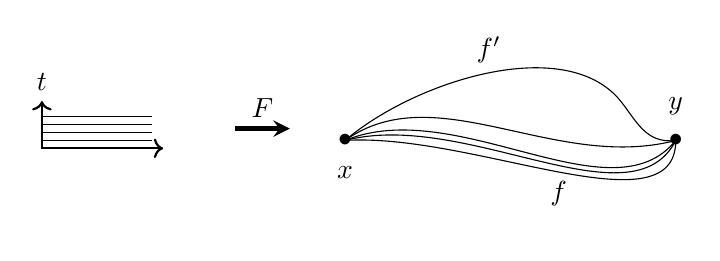
\begin{tikzpicture}[xscale=0.7, yscale=0.5]
		\draw [thick, <->] (1.5, 6.2) node [above] {$t$} -- (1.5, 5) -- (3.7, 5);
		\draw (1.5, 5.2) -- (3.5, 5.2);
		\draw (1.5, 5.4) -- (3.5, 5.4);
		\draw (1.5, 5.6) -- (3.5, 5.6);
		\draw (1.5, 5.8) -- (3.5, 5.8);

		\draw[-stealth, ultra thick] (5, 5.5) -- (6, 5.5) node[midway, above] {$F$};

		\coordinate (x) at (7, 5.2);
		\coordinate (y) at (13, 5.2);
		\node[label=below:$x$]  (x) at (7, 5.2) {$\bullet$};
		\node[label=above:$y$]  (y) at (13, 5.2) {$\bullet$};
		\draw (x.center) to [out=5, in=-90, edge node={node[below] {$f$}}] (y.center);
		\draw (x.center) to [out=20, in=-110] (y.center);
		\draw (x.center) to [out=30, in=-120] (y.center);
		\draw (x.center) to [out=45, in=-160] (y.center);
		\draw (x.center) to [out=50, in=-240, edge node={node[above] {$f'$}}]++(5, 1) to [out=-60, in=-170] (y.center);
	\end{tikzpicture}\end{center}
	Grupoid fundamental $\Pi_1(X)$ dari ruang $X$ didefinisikan sebagai kategori berikut. Objeknya adalah titik-titik dalam $X$, dan untuk setiap $x,y \in X$, himpunan morfisme $\Hom(x,y)$ didefinisikan sebagai himpunan semua kelas homotopi lintasan dari $x$ ke $y$. Komposisi morfisme didefinisikan melalui komposisi kelas lintasan, sedangkan morfisme identitas $\identity_x$ direpresentasikan oleh lintasan konstan $\forall t, \; \identity_x(t) = x$. Untuk morfisme tertentu $f: x \to y$ (yang dipandang sebagai suatu wakil dalam kelas homotopinya), inversnya dapat diambil sebagai lintasan berarah terbalik
	\[ f^{-1}(t) := f(1 - t), \quad 0 \leq t \leq 1. \]

	Dapat diperiksa bahwa semua operasi ini terdefinisi dengan baik dan menjadikan $\Pi_1(X)$ sebuah grupoid. Perhatikan bahwa $\Aut(x) = \Hom(x,x)$ tepat merupakan \emph{grup fundamental} $\pi_1(X, x)$ dengan titik dasar $x$.

	Grup fundamental merupakan invarian penting dalam topologi: kepada setiap ruang $X$ ia mengaitkan suatu struktur aljabar, yaitu grup. Grupoid fundamental dapat dipandang sebagai invarian satu tingkat lebih tinggi: kepada $X$ ia mengaitkan sebuah kategori. Untuk pembahasan lebih lanjut, lihat \cite[Bab 2]{May99}. Namun, pembaca perlu memperhatikan bahwa struktur kategoris $\Pi_1(X)$ masih mengabaikan banyak informasi topologis: selain kelas homotopi lintasan, seharusnya kita memperhitungkan semua homotopi di antara lintasan, kemudian homotopi di antara homotopi, dan seterusnya tanpa akhir. Semua ini harus dicerminkan dalam bahasa kategori yang lebih tinggi.
\end{example}

Akhirnya, kita perkenalkan sebuah konsep yang sederhana dan berguna: kategori lawan.
\begin{definition}\index{kategori!kategori lawan (opposite category)}\index[sym1]{Cop@$\mathcal{C}^\text{op}$}
	Untuk setiap kategori $\mathcal{C}$, \emph{kategori lawan} $\mathcal{C}^\text{op}$ didefinisikan sebagai berikut:
	\begin{compactitem}
		\item $\Obj(\mathcal{C}^{\text{op}}) = \Obj(\mathcal{C})$,
		\item untuk setiap objek $X,Y$, $\Hom_{\mathcal{C}^{\text{op}}}(X, Y) := \Hom_{\mathcal{C}}(Y, X)$,
		\item untuk morfisme $f \in \Hom_{\mathcal{C}^{\text{op}}}(Y, Z)$ dan $g \in \Hom_{\mathcal{C}^{\text{op}}}(X, Y)$, komposisi $f \circ^\text{op} g$ dalam $\mathcal{C}^{\text{op}}$ didefinisikan sebagai komposisi berurutan terbalik $g \circ f$ dalam $\mathcal{C}$,
		\item morfisme identitas didefinisikan sama seperti dalam $\mathcal{C}$.
	\end{compactitem}
\end{definition}
Mudah diperiksa bahwa $\mathcal{C}^\text{op}$ memenuhi definisi kategori dan bahwa $(\mathcal{C}^\text{op})^{\text{op}} = \mathcal{C}$. Singkatnya, konstruksi $\mathcal{C}^\text{op}$ membalikkan semua panah; setelah pembalikan, aksioma teori kategori tetap berlaku. Simetri dalam teori kategori ini disebut pula prinsip dualitas. Sebagai contoh, monomorfisme dalam $\mathcal{C}^\text{op}$ tidak lain adalah epimorfisme dalam $\mathcal{C}$. Dalam menangani banyak sifat kategoris, penggunaan simetri ini dengan tepat dapat sangat menyederhanakan pekerjaan.

\section{Fungtor dan Transformasi Natural}\label{sec:functors}
\begin{definition}[Fungtor]\label{def:functor}\index{fungtor@fungtor (functor)}
	Misalkan $\mathcal{C}', \mathcal{C}$ merupakan kategori. Sebuah fungtor $F: \mathcal{C}' \to \mathcal{C}$ terdiri atas data berikut:
	\begin{enumerate}[(i)]
		\item Peta antarobjek $F: \Obj(\mathcal{C}') \to \Obj(\mathcal{C})$.
		\item Peta antarmorfisme $F: \Mor(\mathcal{C}') \to \Mor(\mathcal{C})$, sedemikian sehingga
			\begin{compactitem}
				\item $F$ berkomutasi dengan peta sumber dan target (yakni $sF=Fs$, $tF=Ft$); secara ekuivalen, untuk setiap $X, Y \in \Obj(\mathcal{C}')$ terdapat peta $F: \Hom_{\mathcal{C}'}(X, Y) \to \Hom_{\mathcal{C}}(FX, FY)$;
				\item $F(g \circ f) = F(g) \circ F(f)$, $F(\identity_X) = \identity_{FX}$.
			\end{compactitem}
	\end{enumerate}
	Untuk $F: \mathcal{C}_1 \to \mathcal{C}_2$, $G: \mathcal{C}_2 \to \mathcal{C}_3$, fungtor komposit $G \circ F: \mathcal{C}_1 \to \mathcal{C}_3$ didefinisikan secara langsung dengan mengambil peta-peta komposit
	\begin{gather*}
		\Obj(\mathcal{C}_1) \xrightarrow{F} \Obj(\mathcal{C}_2) \xrightarrow{G} \Obj(\mathcal{C}_3), \\
		\Mor(\mathcal{C}_1) \xrightarrow{F} \Mor(\mathcal{C}_2) \xrightarrow{G} \Mor(\mathcal{C}_3).
	\end{gather*}
\end{definition}
Dalam literatur lama, fungtor di atas sering disebut fungtor kovarian dari $\mathcal{C}'$ ke $\mathcal{C}$, sedangkan fungtor berbentuk $F: (\mathcal{C}')^\text{op} \to \mathcal{C}$ disebut fungtor kontravarian.

\begin{remark}\label{rem:op-functor}
	Memberikan fungtor dari $\mathcal{C}'$ ke $\mathcal{C}$ sama saja dengan memberikan fungtor dari $(\mathcal{C}')^\text{op}$ ke $\mathcal{C}^\text{op}$. Untuk membedakannya, bagi fungtor $F: \mathcal{C}' \to \mathcal{C}$, fungtor yang bersesuaian di antara kategori lawan dinotasikan dengan $F^\text{op}: (\mathcal{C}')^\text{op} \to \mathcal{C}^\text{op}$.
\end{remark}

\begin{definition}\index{fungtor!penuh (full)}\index{fungtor!surjektif secara esensial (essentially surjective)}\index{fungtor!setia (faithful)}
	Untuk fungtor $F:  \mathcal{C}' \to \mathcal{C}$,
	\begin{enumerate}
		\item $F$ disebut surjektif secara esensial jika setiap objek dalam $\mathcal{C}$ isomorfik dengan suatu $FX$;
		\item $F$ disebut setia jika, untuk semua $X, Y \in \Obj(\mathcal{C}')$, peta $\Hom_{\mathcal{C}'}(X, Y) \to \Hom_{\mathcal{C}}(FX, FY) $ bersifat injektif;
		\item $F$ disebut penuh jika peta di atas bersifat surjektif untuk semua $X, Y \in \Obj(\mathcal{C}')$.
	\end{enumerate}
\end{definition}

\begin{example}\label{eg:functors}
	Fungtor yang digunakan dalam matematika amat banyak; berikut beberapa contoh singkat.
	\begin{enumerate}
		\item Subkategori $\mathcal{C}' \subset \mathcal{C}$ jelas memberikan fungtor inklusi $\iota: \mathcal{C}' \hookrightarrow \mathcal{C}$; fungtor inklusi selalu setia, dan ia penuh jika dan hanya jika $\mathcal{C}'$ merupakan subkategori penuh. Dengan mengambil $\mathcal{C}' = \mathcal{C}$, diperoleh fungtor identitas $\identity_{\mathcal{C}}: \mathcal{C} \to \mathcal{C}$.
		\item Perhatikan kategori grup $\cate{Grp}$. Untuk sebarang grup $G$, kita dapat melupakan struktur grup pada $G$ dan memandangnya sebagai himpunan; homomorfisme grup tentu dapat pula dipandang sebagai peta antarsimpunan. Prosedur ini memberikan \emph{fungtor pelupa} $\cate{Grp} \to \cate{Set}$. Fungtor pelupa untuk struktur lain didefinisikan dengan cara serupa, misalnya $\cate{Top} \to \cate{Set}$ (melupakan struktur topologis ruang), $\cate{Vect}(\Bbbk) \to \cate{Ab}$ (melupakan perkalian skalar pada ruang vektor-$\Bbbk$ $V$ dan hanya memandang grup aditifnya $(V, +)$, dengan $\Bbbk$ sebarang medan), dan sebagainya. Fungtor-fungtor seperti ini jelas setia, tetapi tidak penuh.\index{fungtor pelupa@fungtor pelupa (forgetful functor)}
		\item Perhatikan medan $\Bbbk$ beserta kategori ruang vektor di atasnya $\cate{Vect}(\Bbbk)$. Untuk sebarang ruang vektor-$\Bbbk$ $V$, definisikan ruang dualnya \index[sym1]{$V^\vee$}
			\[ V^\vee := \Hom_\Bbbk(V, \Bbbk) = \{ \Bbbk-\text{peta linear}\; V \to \Bbbk \}. \]
			Setiap peta linear $f: V_1 \to V_2$ menginduksi peta berarah sebaliknya pada ruang dual
			\begin{align*}
				f^\vee: V_2^\vee & \longrightarrow V_1^\vee, \\
				[\lambda: V_2 \to \Bbbk] & \longmapsto \lambda \circ f.
			\end{align*}
			Mudah dilihat bahwa $D: V \mapsto V^\vee$, $f \mapsto f^\vee$ mendefinisikan fungtor $D: \cate{Vect}(\Bbbk)^\text{op} \to \cate{Vect}(\Bbbk)$, dan dapat diperiksa bahwa $D$ setia. Menurut Catatan \ref{rem:op-functor}, kita memiliki fungtor komposit $D D^\text{op}: \cate{Vect}(\Bbbk) \to \cate{Vect}(\Bbbk)$.
			
			Dengan membatasi $D$ pada ruang vektor berdimensi hingga, diperoleh fungtor $D: \cate{Vect}_f(\Bbbk)^\text{op} \to \cate{Vect}_f(\Bbbk)$ dan $D D^\text{op}: \cate{Vect}_f(\Bbbk) \to \cate{Vect}_f(\Bbbk)$. Keduanya disebut, berturut-turut, fungtor dual dan fungtor dual ganda.
		\item Untuk sebarang grup $G$, definisikan subgrup turunan $G_\text{der}$ sebagai subgrup normal yang dibangkitkan oleh himpunan $\{xyx^{-1} y^{-1} : x,y \in G \}$. Grup hasil bagi $G/G_\text{der}$ merupakan grup abelian dan disebut abelianisasi dari $G$ (lihat Lema \ref{prop:abelianization}). Untuk sebarang homomorfisme grup $\varphi: G \to H$, dari definisi terlihat bahwa $\varphi(G_\text{der}) \subset H_\text{der}$; karena itu, $\varphi$ menginduksi homomorfisme grup abelian $\bar{\varphi}: G/G_\text{der} \to H/H_\text{der}$. Mudah diperiksa bahwa $G \mapsto G/G_\text{der}$, $\varphi \mapsto \bar{\varphi}$ mendefinisikan fungtor abelianisasi $\cate{Grp} \to \cate{Ab}$. Fungtor abelianisasi tidak setia.
		\item Kepada setiap ruang topologis bertitik dasar $(X,x)$, kaitkan grup fundamental $\pi_1(X, x)$; ini memberikan fungtor $\cate{Top}_\bullet \to \cate{Grp}$. Masih banyak contoh lain dalam topologi aljabar; misalnya, grup homologi suatu ruang $X \mapsto H_n(X; \Z)$ memberikan keluarga fungtor $H_n: \cate{Top} \to \cate{Ab}$, dengan $n \in \Z_{\geq 0}$, sedangkan grup kohomologi memberikan fungtor $H^n: \cate{Top}^\text{op} \to \cate{Ab}$.
	\end{enumerate}
\end{example}

\begin{definition}[Transformasi natural, atau morfisme antarfungtor]\index{transformasi natural@transformasi natural (natural transformation)}
	Di antara fungtor $F, G: \mathcal{C}' \to \mathcal{C}$, suatu transformasi natural $\theta$ adalah keluarga morfisme
	\[ \theta_X \in \Hom_{\mathcal{C}}(FX, GX), \quad X \in \Obj(\mathcal{C}'), \]
	sedemikian sehingga, dalam $\mathcal{C}'$, diagram berikut komutatif untuk setiap morfisme $f: X \to Y$
	\begin{equation}\label{eqn:naturaltrans-def}\begin{tikzcd}
		FX \arrow[r, "\theta_X"] \ar[d, "Ff"'] & GX \arrow[d, "Gf"] \\
		FY \arrow[r, "\theta_Y"'] & GY .
	\end{tikzcd}\end{equation}
	Transformasi natural di atas ditulis sebagai $\theta: F \to G$, atau digambarkan dengan diagram
	\[ \begin{tikzcd}
		\mathcal{C}' \arrow[bend left=50, r, "F", ""' name=U] \arrow[bend right=50, r, "G"', "" name=D] & \arrow[Rightarrow, to path=(U) -- (D) \tikztonodes, "\theta"] \mathcal{C}.
	\end{tikzcd} \]
\end{definition}
Diagram dengan panah ganda $\Rightarrow$ di atas kadang-kadang disebut pula sel-$2$; lihat \S\ref{sec:2-cat}. Sudut pandang yang barangkali lebih bermanfaat ialah membayangkan $\theta$ sebagai suatu homotopi dari $F$ ke $G$.

\begin{convention}\label{con:naturaltrans-morphism}\index{natural@natural}\index{kanonik@kanonik}
	Kita juga menyebut transformasi natural $\theta: F \to G$ sebagai morfisme dari fungtor $F$ ke $G$. Dalam penerapan, kerangka teori kategori yang ketat sering dihilangkan, dan cukup dikatakan bahwa morfisme $\theta_X: FX \to GX$ bersifat \emph{natural}, \emph{kanonik}, atau memenuhi \emph{fungtorialitas} terhadap peubah $X$. Dalam praktik, isomorfisme natural sering langsung ditulis sebagai tanda sama dengan $=$.
\end{convention}

Selanjutnya kita perkenalkan beberapa operasi pada transformasi natural, termasuk komposisi vertikal dan horizontal.\index{transformasi natural!komposisi}
\begin{itemize}
	\item Perhatikan tiga fungtor dari $\mathcal{C}'$ ke $\mathcal{C}$ beserta morfisme antarfungtor $\theta: F \to  G$,  $\psi: G \to H$. Komposisi vertikal $\psi \circ \theta$ didefinisikan sebagai $\{ \psi_X \circ \theta_X : X \in \Obj(\mathcal{C}') \}$, dan digambarkan sebagai berikut:
	\[\begin{tikzcd}
		\mathcal{C}'
			\arrow[bend left=70, rr, "F", ""' name=U]
			\arrow[rr, "G" name=MM, ""' name=M]
			\arrow[bend right=70, rr, "" name=D, "H"'] & &
		\arrow[Rightarrow, to path=(U) -- (MM) \tikztonodes, "\theta"] \arrow[Rightarrow, to path=(M) -- (D) \tikztonodes, "\psi"] \mathcal{C} 
	\end{tikzcd} \quad \text{dikomposisikan menjadi} \quad \begin{tikzcd}
		\mathcal{C}'
		\arrow[bend left=50, rr, "F", ""' name=U]
		\arrow[bend right=50, rr, "" name=D, "H"']
		& & \arrow[Rightarrow, to path=(U) -- (D) \tikztonodes, "\psi \circ \theta"] \mathcal{C} .
	\end{tikzcd}\]
	\item Perhatikan fungtor-fungtor
	$\begin{tikzcd}
		\mathcal{C}'' \arrow[bend left=30, r, "F_1"] \arrow[bend right=30, r, "F_2"] & \mathcal{C}' \arrow[bend left=30, r, "G_1"] \arrow[bend right=30, r, "G_2"] & \mathcal{C}
	\end{tikzcd}$
	dan morfisme $\theta: F_1 \to F_2$, $\psi: G_1 \to G_2$. Kita akan mendefinisikan komposisi horizontal $\psi \circ \theta: G_1 \circ F_1 \to G_2 \circ F_2$. Pertama, perhatikan bahwa bagi semua $X \in \Obj(\mathcal{C}'')$, dari naturalitas $\psi$, diagram
	\begin{equation}\label{eqn:horizontal-comp}\begin{tikzcd}
		G_1 F_1(X) \arrow[r, "{\psi_{F_1 X}}"] \arrow[d, "{G_1(\theta_X)}"'] & G_2 F_1(X) \arrow[d, "{G_2(\theta_X)}"] \\
		G_1 F_2(X) \arrow[r, "{\psi_{F_2 X}}"'] & G_2 F_2(X)
	\end{tikzcd}\end{equation}
	komutatif. Komposisi sepanjang diagonal $\searrow$ dinotasikan dengan $(\psi \circ \theta)_X : G_1 F_1 (X) \to G_2 F_2 (X)$; inilah komposisi horizontal yang dikehendaki. Kita akan segera membuktikan naturalitasnya, dan pembaca dapat memanfaatkan kesempatan ini untuk membiasakan diri menggunakan diagram komutatif. Diagramnya ialah:
	\[ \begin{tikzcd}
		\mathcal{C}'' \arrow[bend left=50, r, "F_1", ""' name=LU] \arrow[bend right=50, r, "" name=LD, "F_2"'] &
		\mathcal{C}' \arrow[bend left=50, r, "G_1", ""' name=RU] \arrow[bend right=50, r, "" name=RD, "G_2"'] &
		\arrow[Rightarrow, to path=(LU) -- (LD) \tikztonodes, "\theta"] \arrow[Rightarrow, to path=(RU) -- (RD) \tikztonodes, "\psi"] \mathcal{C}
	\end{tikzcd} \quad \text{dikomposisikan menjadi} \quad \begin{tikzcd}
		\mathcal{C}''
		\arrow[bend left=50, rr, "G_1 F_1", ""' name=U]
		\arrow[bend right=50, rr, "" name=D, "G_2 F_2"']
		& & \arrow[Rightarrow, to path=(U) -- (D) \tikztonodes, "\psi \circ \theta"] \mathcal{C} .
	\end{tikzcd} \]
	\item Komposisi horizontal mempunyai kasus khusus berikut. Perhatikan
	\[\begin{tikzcd}
		\mathcal{C}_1 \arrow[r, "H"] & \mathcal{C}_2 \arrow[bend left=50, r, "F", ""' name=U] \arrow[bend right=50, r, "" name=D, "G"'] & \mathcal{C}_3 \arrow[Rightarrow, to path=(U)--(D) \tikztonodes, "\theta"] \arrow[r, "K"] & \mathcal{C}_4 .
    \end{tikzcd} \]
	Pertama perhatikan tiga unsur di sebelah kiri: notasi $\theta H: FH \to GH$ kita gunakan sebagai singkatan bagi komposisi horizontal $\theta \circ \identity_{H}$; secara konkret, $(\theta H)_X = \theta_{HX} : FH(X) \to GH(X)$. Tiga unsur di sebelah kanan diperlakukan serupa: tuliskan $K\theta: KF \to KG$ untuk komposisi horizontal $\identity_K \circ \theta$, sehingga $(K\theta)_X = K(\theta_X): KF(X) \to KG(X)$.
\end{itemize}
Perhatikan bahwa kita menggunakan lambang yang sama $\circ$ untuk komposisi vertikal maupun horizontal; bila ada kemungkinan rancu, akan diberikan penjelasan tersendiri.

\begin{lemma}\label{prop:naturaltrans-associativity}
	Komposisi vertikal dan horizontal $\{ (\psi \circ \theta)_X \}_X$ yang didefinisikan di atas sama-sama merupakan morfisme antarfungtor, dan masing-masing memenuhi hukum asosiatif ketat $(\phi \circ \psi) \circ \theta = \phi \circ (\psi \circ \theta)$. Di antara komposisi vertikal dan horizontal berlaku hubungan berikut: untuk diagram
	\[\begin{tikzcd}
		\mathcal{C}_1
		\arrow[bend left=70, rr, ""' name=U]
		\arrow[rr, "" name=MM, ""' name=M]
		\arrow[bend right=70, rr, "" name=D] & &
		\arrow[Rightarrow, to path=(U) -- (MM) \tikztonodes, "\theta"] \arrow[Rightarrow, to path=  (M) -- (D) \tikztonodes, "\psi"] \mathcal{C}_2
		\arrow[bend left=70, rr, ""' name=V]
		\arrow[rr, "" name=NN, ""' name=N]
		\arrow[bend right=70, rr, "" name=E] & &
		\arrow[Rightarrow, to path=(V) -- (NN) \tikztonodes, "\theta'"] \arrow[Rightarrow, to path=  (N) -- (E) \tikztonodes, "\psi'"] \mathcal{C}_3 ,
	\end{tikzcd} \]
	berlaku hukum pertukaran berikut
	\[ \left( \psi' \underset{\text{vertikal}}{\circ} \theta'\right) \underset{\text{horizontal}}{\circ} \left( \psi \underset{\text{vertikal}}{\circ} \theta\right) = \left( \psi' \underset{\text{horizontal}}{\circ} \psi \right) \underset{\text{vertikal}}{\circ} \left( \theta' \underset{\text{horizontal}}{\circ} \theta\right).  \]
\end{lemma}
\begin{proof}
	Pernyataan mengenai komposisi vertikal mudah; berikut kita buktikan bahwa komposisi horizontal merupakan morfisme antarfungtor. Kita gunakan notasi sebelumnya. Dalam $\mathcal{C}''$, untuk morfisme $f: X \to Y$, perhatikan diagram yang berasal dari \eqref{eqn:horizontal-comp}
	\[\begin{tikzcd}
		G_1 F_1 (X) \arrow[r, "G_1 \theta_X"] \arrow[d, "G_1 F_1 f"'] & G_1 F_2 (X) \arrow[r, "{\psi_{F_2 X}}"] \arrow[d, "G_1 F_2 f"] & G_2 F_2 (X) \arrow[d, "G_2 F_2 f"] \\
		G_1 F_1 (Y) \arrow[r, "{G_1 \theta_Y}"'] & G_1 F_2 (Y) \arrow[r, "{\psi_{F_2 Y}}"'] & G_2 F_2 (Y) .
	\end{tikzcd} \]
	Menurut definisi, komposisi panah horizontal di baris atas dan bawah masing-masing adalah $(\psi \circ \theta)_X$ dan $(\psi \circ \theta)_Y$. Karena $\theta$ merupakan transformasi natural dan $G_1$ sebuah fungtor, persegi kiri komutatif; karena $\psi$ merupakan transformasi natural, persegi kanan pun komutatif. Dengan mengomposisikan panah-panah per bagian, diperoleh bahwa seluruh persegi besar komutatif; inilah sifat yang diperlukan bagi $ \psi \circ \theta$.

	Sekarang kita buktikan asosiativitas komposisi horizontal. Perhatikan morfisme-morfisme antarfungtor
	\[\begin{tikzcd}
		\mathcal{C}''' \arrow[bend left=50, r, "F_1", ""' name=LU] \arrow[bend right=50, r, "" name=LD, "F_2"'] &
		\mathcal{C}'' \arrow[bend left=50, r, "G_1", ""' name=MU] \arrow[bend right=50, r, "" name=MD, "G_2"'] &
		\mathcal{C}' \arrow[bend left=50, r, "H_1", ""' name=RU] \arrow[bend right=50, r, "" name=RD, "H_2"'] &
		\arrow[Rightarrow, to path=(LU) -- (LD) \tikztonodes, "\theta"]
		\arrow[Rightarrow, to path=(MU) -- (MD) \tikztonodes, "\psi"]
		\arrow[Rightarrow, to path=(RU) -- (RD) \tikztonodes, "\phi"]
		\mathcal{C} .
	\end{tikzcd} \]
	Untuk sebarang $X \in \Obj(\mathcal{C}''')$, perhatikan diagram
	\[\begin{tikzcd}[row sep=small]
		& & H_1 G_2 F_2(X) \arrow[rd] & \\
		H_1 G_1 F_1(X) \arrow[r] & H_1 G_2 F_1(X) \arrow[ru] \arrow[rd] & & H_2 G_2 F_2(X) . \\
		& & H_2 G_2 F_1(X) \arrow[ru] &
	\end{tikzcd}\]
	Dengan menerapkan naturalitas $\phi$ pada $G_2 F_1(X) \to G_2 F_2(X)$, bagian berbentuk belah ketupat diketahui komutatif. Komposisi sepanjang lintasan
	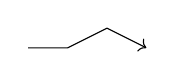
\begin{tikzpicture}[scale=0.5, baseline=(X)]
		\draw[->] (0,0) -- (1,0) -- (2, 0.5) -- (3, 0);
		\coordinate (X) at (0,0);
	\end{tikzpicture}
	menghasilkan $(\phi \circ (\psi \circ \theta))_X$. Sementara itu, komposisi sepanjang lintasan
	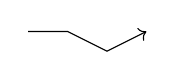
\begin{tikzpicture}[scale=0.5, baseline=(X)]
		\draw[->] (0,0) -- (1,0) -- (2, -0.5) -- (3, 0);
		\coordinate (X) at (0, -0.2);
	\end{tikzpicture}
	menghasilkan $((\phi \circ \psi) \circ \theta)_X$; di sini kita masih perlu menggunakan diagram komutatif \eqref{eqn:horizontal-comp}. Asosiativitas pun terbukti.

	Persamaan terakhir dapat diperoleh secara serupa dengan menelusuri diagram; rinciannya diserahkan kepada pembaca yang berminat.
\end{proof}

Setiap fungtor $F$ mempunyai morfisme identitas ke dirinya sendiri, $\identity_F : F \to F$. Diberikan morfisme antarfungtor $\theta: F_1 \to F_2$, jika morfisme $\psi: F_2 \to F_1$ memenuhi $\psi \circ \theta = \identity_{F_1}$, $\theta \circ \psi = \identity_{F_2}$, maka $\psi$ disebut invers dari $\theta$. Morfisme invertibel disebut isomorfisme antarfungtor dan ditulis $\theta: F_1 \rightiso F_2$. Langsung dari definisi terlihat bahwa invers $\theta$, jika ada, bersifat tunggal dan dinotasikan dengan $\theta^{-1}$; invers ini tidak lain diperoleh dengan mengambil invers ``titik demi titik'' dalam kategori: $(\theta^{-1})_X := (\theta_X)^{-1}: F_2 X \rightiso F_1 X$. Demikian pula, morfisme $\theta$ invertibel jika dan hanya jika setiap $\theta_X$ invertibel. Mudah dilihat bahwa komposisi vertikal maupun horizontal dari isomorfisme tetap merupakan isomorfisme. Pernyataan ekuivalen bagi isomorfisme antarfungtor $\theta: F_1 \rightiso F_2$ ialah bahwa $\theta_X: F_1 X \rightiso F_2 X$ merupakan \emph{isomorfisme natural} atau \emph{isomorfisme kanonik} terhadap peubah $X$.

\begin{definition}[Ekuivalensi]\label{def:cat-equivalence}\index{ekuivalensi kategori@ekuivalensi kategori (equivalence)}\index{fungtor!kuasi-invers (quasi-inverse)}
	Jika sepasang fungtor
	\begin{tikzcd}
		\mathcal{C}_1 \arrow[bend left=20, r, "F"] & \mathcal{C}_2 \arrow[bend left=20, l, "G"]
	\end{tikzcd}
	memenuhi sifat berikut: terdapat isomorfisme antarfungtor $\theta: FG \rightiso \identity_{\mathcal{C}_2}$, $\psi: GF \rightiso \identity_{\mathcal{C}_1}$, maka $G$ disebut, bagi $F$, \emph{fungtor kuasi-invers}, dan $F$ disebut ekuivalensi dari kategori $\mathcal{C}_1$ ke $\mathcal{C}_2$, atau singkatnya suatu \emph{ekuivalensi}.

	Jika lebih lanjut $FG = \identity_{\mathcal{C}_2}$, $GF = \identity_{\mathcal{C}_1}$, maka $F$ disebut \emph{isomorfisme} antarkategori, sedangkan $G$ disebut \emph{invers} dari $F$.
\end{definition}
Mudah dibuktikan bahwa komposisi ekuivalensi tetap merupakan ekuivalensi; rinciannya dijadikan latihan.

\begin{example}
	Misalkan $\cate{CHaus}$ adalah kategori ruang topologis kompak Hausdorff, dan $C^*\dcate{CommAlg}$ kategori aljabar-$C^*$ komutatif berunsur satuan (dengan morfisme berupa homomorfisme-$\ast$ yang mempertahankan unsur satuan). Versi komutatif teorema Gelfand--Naimark menyatakan bahwa fungtor-fungtor
	\[ \begin{tikzcd}[row sep=tiny]
		\cate{CHaus}^{\text{op}} \arrow[yshift=0.7ex]{r} & C^*\dcate{CommAlg} \arrow[yshift=-0.7ex]{l} \\
		X \arrow[mapsto]{r} & C(X): \text{ruang fungsi kontinu bernilai kompleks} \\
		\mathfrak{M}_A: \text{ ruang ideal maksimal} & A \arrow[mapsto]{l}
	\end{tikzcd} \]
	saling kuasi-invers: transformasi Gelfand $a \mapsto \hat{a}$ memberikan isomorfisme natural $A \rightiso C(\mathfrak{M}_A)$; lihat \cite[Teorema 5.4.8]{Zh2}. Isomorfisme natural pada arah sebaliknya, $X \rightiso \mathfrak{M}_{C(X)}$, relatif lebih mudah; lihat \cite[Teorema 5.3.2]{Zh2}.
\end{example}

\begin{proposition}
	Jika $G, G'$ merupakan kuasi-invers dari fungtor $F: \mathcal{C}_1 \to \mathcal{C}_2$, maka terdapat isomorfisme antarfungtor $G \simeq G'$.
\end{proposition}
\begin{proof}
	Komposisi horizontal transformasi natural memberikan $G \xleftarrow[\sim]{\psi' \circ \identity_G} (G'F)G = G'(FG) \xrightarrow[\sim]{\identity_{G'} \circ \theta} G'$.
\end{proof}

\begin{remark}\label{rem:strict-or-not}
	Kita telah mendefinisikan konsep invers bagi morfisme antarobjek dan morfisme antarfungtor (transformasi natural); invers tersebut, jika ada, bersifat tunggal, dan dari sinilah isomorfisme antarobjek atau antarfungtor didefinisikan. Konsep invers dapat pula didefinisikan bagi fungtor, dan fungtor invers, jika ada, bersifat tunggal. Sebaliknya, dua fungtor kuasi-invers dapat berbeda hingga suatu isomorfisme. Praktik menunjukkan bahwa konsep isomorfisme kategori kurang berguna, sedangkan konsep ekuivalensi muncul di mana-mana. Hal ini mencerminkan suatu kaidah praktis dalam teori kategori: pada tingkat fungtor, isomorfisme (seperti $\theta: FG \rightiso \identity$ di atas) hampir selalu lebih berguna daripada kesamaan ketat (seperti $FG = \identity$ di atas). Namun, isomorfisme itu pun tidak boleh sebarang; syarat yang diperlukan biasanya disebut koherensi. Dalam kasus ekuivalensi, pembaca mungkin telah merasakan dalam argumen sebelumnya bahwa konsep kuasi-invers agak longgar; Teorema \ref{prop:adjoint-equivalence} akan memberikan suatu penyempurnaan yang disebut \emph{ekuivalensi adjoin}. \index{ekuivalensi adjoin@ekuivalensi adjoin (adjoint equivalence)}
\end{remark}

Subkategori penuh $\mathcal{C}' \subset \mathcal{C}$ disebut, bagi $\mathcal{C}$, suatu \emph{kerangka} jika setiap objek dalam $\mathcal{C}$, katakan $X$, memiliki isomorfisme $X \rightiso Y \in \Obj(\mathcal{C}')$, dan $Y \in \Obj(\mathcal{C}')$ tersebut tunggal. Kategori yang merupakan kerangka bagi dirinya sendiri disebut \emph{kategori skeletal}.\index{kategori!kerangka (skeleton)}

\begin{lemma}\label{prop:skeletal-cat-isom}
	Setiap kategori $\mathcal{C}$ memiliki suatu kerangka $\mathcal{C}'$, dan fungtor inklusi $\iota: \mathcal{C}' \hookrightarrow \mathcal{C}$ merupakan ekuivalensi. Setiap fungtor penuh, setia, dan surjektif secara esensial di antara kategori skeletal merupakan isomorfisme.
\end{lemma}
\begin{proof}
	Kita buktikan dahulu bagian pertama. Dengan aksioma pilihan, pilih satu wakil dari setiap kelas isomorfisme dalam $\Obj(\mathcal{C})$, lalu nyatakan subkategori penuh yang dibentuk oleh wakil-wakil tersebut sebagai $\mathcal{C}'$. Demikian pula, untuk setiap $X \in \Obj(\mathcal{C})$, kita dapat memilih isomorfisme $\theta_X: X \rightiso \kappa(X) $, dengan $\kappa(X) \in \Obj(\mathcal{C}')$; tanpa mengurangi keumuman, andaikan bagi $X \in \Obj(\mathcal{C}')$ berlaku $\theta_X = \identity_X$. Ada tepat satu cara memperluas $\kappa: \Obj(\mathcal{C}) \to \Obj(\mathcal{C}')$ menjadi fungtor sedemikian sehingga $\theta: \identity_{\mathcal{C}} \rightiso \iota \kappa$: tetapkan
	\[ \kappa(f) := \theta_Y \circ f \circ \theta_X^{-1} \in \Hom_{\mathcal{C}'}(\kappa(X), \kappa(Y)), \quad f \in \Hom_{\mathcal{C}}(X, Y). \]
	Di sisi lain, kita memiliki kesamaan fungtor $\kappa\iota = \identity_{\mathcal{C}'}$. Jadi, $\kappa$ merupakan fungtor kuasi-invers dari $\iota$.
	
	Untuk bagian kedua, misalkan $F: \mathcal{C}_1 \to \mathcal{C}_2$ adalah fungtor penuh, setia, dan surjektif secara esensial di antara kategori skeletal. Untuk sebarang objek dalam $\mathcal{C}_2$, katakan $Z$, terdapat $X$ sedemikian sehingga $Z \simeq FX$, dan karena itu $Z = FX$. Objek $X$ seperti ini tunggal, sebab sifat penuh dan setia bersama $FX \simeq FX'$ mengakibatkan $X \simeq X'$. Dengan demikian, $F$ bijektif pada himpunan objek, sehingga fungtor inversnya $G$ dapat didefinisikan.
\end{proof}

\begin{theorem}\label{prop:functor-equiv-criterion}\index{ekuivalensi kategori@ekuivalensi kategori (equivalence)}
	Untuk fungtor $F: \mathcal{C}_1 \to \mathcal{C}_2$, pernyataan-pernyataan berikut ekuivalen.
	\begin{compactenum}
		\item $F$ merupakan ekuivalensi kategori,
		\item $F$ merupakan fungtor penuh, setia, dan surjektif secara esensial.
	\end{compactenum}
\end{theorem}
\begin{proof}
	Andaikan $F$ merupakan ekuivalensi kategori. Ambil fungtor kuasi-invers $G: \mathcal{C}_2 \to \mathcal{C}_1$ beserta $GF \xrightarrow[\sim]{\psi} \identity_{\mathcal{C}_1}$, $FG \xrightarrow[\sim]{\phi} \identity_{\mathcal{C}_2}$. Untuk setiap objek dalam $\mathcal{C}_2$, katakan $Z$, terdapat $\phi_Z: F(GZ) \rightiso Z$, sehingga $F$ surjektif secara esensial; dengan cara yang sama, $G$ juga surjektif secara esensial. Perhatikan bahwa
	\[\begin{tikzcd}[row sep=tiny, column sep=small]
		\Hom(X,Y) \arrow[r, "F"] & \Hom(FX, FY) \arrow[r, "G"] & \Hom(GF(X), GF(Y)) \arrow[r, "\sim"] & \Hom(X, Y) \\
		f \arrow[mapsto, r] & Ff \arrow[mapsto, r] & GF(f) \arrow[mapsto, r] & \psi_Y GF(f) \psi_X^{-1}
	\end{tikzcd}\]
	komposisinya merupakan peta identitas; jadi, panah pertama $F$ pada diagram mempunyai invers kiri, sedangkan panah kedua $G$ mempunyai invers kanan. Dengan menukar peran $F, G$, terlihat bahwa apabila $X, Y \in \Obj(\mathcal{C}_1)$ termasuk dalam citra $G$, peta $\Hom(X, Y) \xrightarrow{F} \Hom(FX, FY)$ mempunyai invers kanan. Akan tetapi, setiap objek dalam $\mathcal{C}_1$ isomorfik dengan suatu objek dalam citra $G$; karena itu, $F$ merupakan fungtor penuh dan setia.

	Sekarang kita buktikan arah sebaliknya. Dengan Lema \ref{prop:skeletal-cat-isom}, ambil kerangka $\iota_i: \mathcal{C}'_i \rightarrow \mathcal{C}_i$ beserta fungtor kuasi-inversnya $\kappa_i$ (di sini $i=1,2$). Fungtor $F' := \kappa_2 \circ F \circ \iota_1: \mathcal{C}'_1 \to \mathcal{C}'_2$ tetap penuh, setia, dan surjektif secara esensial; jadi, $F'$ merupakan isomorfisme kategori. Tetapkan $G := \iota_1 \circ F'^{-1} \circ \kappa_2$; maka
	\begin{gather*}
		GF = \iota_1  F'^{-1} \kappa_2 F \simeq \iota_1  F'^{-1} \underbracket{\kappa_2 F \iota_1}_{= F'} \kappa_1 = \iota_1 \kappa_1 \simeq \identity_{\mathcal{C}_1}, \\
		FG = F \iota_1  F'^{-1} \kappa_2 \simeq \iota_2 \underbracket{\kappa_2 F \iota_1}_{= F'}  F'^{-1} \kappa_2 = \iota_2 \kappa_2 \simeq \identity_{\mathcal{C}_2}.
	\end{gather*}
	Di sini kita telah menggunakan komposisi horizontal transformasi natural.
\end{proof}

\begin{example}\label{eg:vectf-duality}
	Masih dengan medan $\Bbbk$, perhatikan kembali kategori ruang vektor di atasnya $\cate{Vect}(\Bbbk)$ beserta subkategorinya $\cate{Vect}_f(\Bbbk)$. Dalam Contoh \ref{eg:functors}, telah didefinisikan fungtor dual ganda $D D^\text{op}: \cate{Vect}(\Bbbk) \to \cate{Vect}(\Bbbk)$. Untuk setiap ruang vektor $V$, terdapat peta evaluasi
	\begin{align*}
		\text{ev}: V & \longrightarrow DD^\text{op} V = (V^\vee)^\vee \\
		v & \longmapsto [\lambda \mapsto \lambda(v)].
	\end{align*}
	Untuk sebarang peta linear $f: V \to W$, dari definisi $f^\vee$ tidak sulit diperiksa bahwa diagram berikut
	\[\begin{tikzcd}
		V \arrow[r, "\text{ev}"] \ar[d, "f"'] & DD^\text{op} V \arrow[d, "{DD^\text{op} f}"] \\
		W \ar[r, "\text{ev}"'] & DD^\text{op} W
	\end{tikzcd} \]
	komutatif, sehingga diperoleh $\text{ev}: \identity \to D D^\text{op}$. Mudah dilihat bahwa $\text{ev}: V \to D D^\text{op} V$ selalu injektif; bahkan dapat dibuktikan bahwa $\text{ev}$ bijektif jika dan hanya jika $V$ berdimensi hingga. Setelah semuanya dibatasi pada subkategori penuh $\cate{Vect}_f(\Bbbk)$, diperoleh isomorfisme
	\[ \text{ev}: \identity_{\cate{Vect}_f(\Bbbk)} \rightiso D D^\text{op}. \]
	Jika rumus yang sama ditafsirkan dalam kategori lawan, diperoleh
	\[ \identity_{\cate{Vect}_f(\Bbbk)^\text{op}} \rightiso D^\text{op} D. \]
	Jadi, fungtor $D: \cate{Vect}_f(\Bbbk)^\text{op} \to \cate{Vect}_f(\Bbbk)$ merupakan ekuivalensi antarkategori, sedangkan $D^\text{op}: \cate{Vect}_f(\Bbbk) \to \cate{Vect}_f(\Bbbk)^\text{op}$ merupakan kuasi-inversnya.
\end{example}

\begin{example}
	Pilih sebuah medan $\Bbbk$, dan definisikan kategori $\cate{Mat}$ sebagai berikut: objek-objeknya adalah $\Z_{\geq 0}$; untuk sebarang objek $n, m \in \Z_{\geq 0}$, definisikan $\Hom(n, m) := M_{m \times n}(\Bbbk)$ sebagai himpunan semua matriks di atas medan $\Bbbk$ yang berukuran $m \times n$, yaitu $A = (a_{ij})_{\substack{1 \leq i \leq m \\ 1 \leq j \leq n}}$. Dengan konvensi $M_{0 \times n}(\Bbbk) = M_{m \times 0}(\Bbbk) := \{0\}$, komposisi morfisme didefinisikan sebagai perkalian matriks biasa
	\begin{align*}
		\Hom(n, m) \times \Hom(m, k) & \longrightarrow \Hom(n, k) \\
		(A, B) & \longmapsto BA .
	\end{align*}

	Definisikan fungtor $F: \cate{Mat} \to \cate{Vect}_f(\Bbbk)$ sebagai berikut: tetapkan $F(n) = \Bbbk^{\oplus n} := M_{n \times 1}(\Bbbk)$; untuk $A \in \Hom(n, m)$, peta linear $FA: \Bbbk^{\oplus n} \to \Bbbk^{\oplus m}$ adalah perkalian matriks $v \mapsto Av$. Kita menyatakan bahwa $F$ merupakan ekuivalensi kategori.

	Semua ini hanyalah aljabar linear yang tampak lebih megah daripada sebenarnya. Pertama, perhatikan bahwa $F: \Hom(n, m) \to \Hom_\Bbbk(\Bbbk^{\oplus n}, \Bbbk^{\oplus m})$ merupakan bijeksi; ini tidak lain adalah representasi matriks suatu peta linear. Selanjutnya, dari $V \simeq \Bbbk^{\oplus \dim V}$ (dengan $V$ ruang vektor-$\Bbbk$) diketahui bahwa $F$ penuh, setia, dan surjektif secara esensial; menurut Teorema \ref{prop:functor-equiv-criterion}, fungtor tersebut merupakan ekuivalensi kategori.
\end{example}

\section{Kategori Fungtor}\label{sec:functor-category}
Pertama-tama kita definisikan konsep produk dan koproduk (juga disebut gabungan saling lepas) kategori; konsep-konsep ini sangat berguna untuk menyatakan sejumlah sifat kategori.

Ingat kembali Konvensi \ref{con:U-small}: kecuali dinyatakan lain, kategori yang dibahas berikut ini semuanya merupakan kategori-$\mathcal{U}$, dengan $\mathcal{U}$ semesta yang telah dipilih. Himpunan yang termasuk dalam $\mathcal{U}$ disebut himpunan-$\mathcal{U}$.

\begin{definition}\index{kategori!produk, koproduk}
	Misalkan $I$ merupakan himpunan-$\mathcal{U}$ dan $\{\mathcal{C}_i : i \in I \}$ suatu keluarga kategori.
	\begin{itemize}
		\item Kategori produk $\prod_{i \in I} \mathcal{C}_i$ didefinisikan sebagai berikut:
			\begin{align*}
				\Obj\left( \prod_{i \in I} \mathcal{C}_i \right) & := \prod_{i \in I} \Obj(\mathcal{C}_i), \\
				\Hom_{\prod_{i \in I} \mathcal{C}_i}( (X_i)_i, (Y_i)_i ) & := \prod_{i \in I} \Hom_{\mathcal{C}_i}(X_i, Y_i),
			\end{align*}
			dengan $(X_i)_i$ menyatakan suatu unsur dari $\prod_{i \in I} \Obj(\mathcal{C}_i)$. Komposisi morfisme didefinisikan per komponen.
		\item Kategori koproduk (juga disebut gabungan saling lepas) $\coprod_{i \in I} \mathcal{C}_i$ didefinisikan sebagai berikut:
			\begin{align*}
				\Obj\left( \coprod_{i \in I} \mathcal{C}_i \right) & := \coprod_{i \in I} \Obj(\mathcal{C}_i), \\
				\Hom_{\coprod_{i \in I} \mathcal{C}_i}(X_j, X'_k) & :=
				\begin{cases}
					\Hom_{\mathcal{C}_j}(X_j, X'_k), & j = k, \\
					\emptyset, & j \neq k;
				\end{cases}
			\end{align*}
			di sini, untuk setiap $j \in I$, berlaku $X_j, X'_j \in \Obj(\mathcal{C}_j)$. Komposisi morfisme didefinisikan secara terpisah di dalam setiap $\mathcal{C}_i$.
	\end{itemize}
\end{definition}
Karena $I$ diasumsikan sebagai himpunan-$\mathcal{U}$, kategori yang dikonstruksi di atas tetap merupakan kategori-$\mathcal{U}$; jika setiap $\mathcal{C}_i$ merupakan kategori kecil-$\mathcal{U}$, maka produk dan koproduknya pun demikian.

Kita memiliki keluarga fungtor proyeksi $\pr_j: \prod_{i \in I} \mathcal{C}_i \to \mathcal{C}_j$, yang memetakan $(X_i)_i$ ke $X_j$ dan, pada tingkat morfisme, secara serupa memproyeksikan ke komponen ke-$j$. Demikian pula, didefinisikan keluarga fungtor inklusi $\iota_j: \mathcal{C}_j \to \coprod_{i \in I} \mathcal{C}_i$, yang menyisipkan $\mathcal{C}_j$ dengan cara yang jelas sebagai subkategori penuh.

Khususnya, dengan mengambil $I$ sebagai himpunan hingga, kita dapat mendefinisikan $\mathcal{C}_1 \times \cdots \times \mathcal{C}_n$ dan $\mathcal{C}_1 \sqcup \cdots \sqcup \mathcal{C}_n$.

\begin{definition}
	Fungtor berbentuk $F: \mathcal{C}_1 \times \mathcal{C}_2 \to \mathcal{C}$ disebut fungtor biner. Fungtor banyak peubah $\mathcal{C}_1 \times \cdots \times \mathcal{C}_n \to \mathcal{C}$ didefinisikan secara serupa.
\end{definition}

\begin{example}[Fungtor $\Hom$]\label{eg:Hom-functor} \index[sym1]{HomC}
	Untuk kategori $\mathcal{C}$, pemetaan $(X,Y)\mapsto\Hom_{\mathcal{C}}(X,Y)$ mendefinisikan fungtor biner
	\[ \Hom_{\mathcal{C}}: \mathcal{C}^\text{op} \times \mathcal{C}  \to \cate{Set}. \]
	Memang, setiap pasangan morfisme $f: X' \to X$, $g: Y \to Y'$ dalam $\mathcal{C}$ menginduksi
	\begin{align*}
		\Hom_{\mathcal{C}}(X, Y) & \longrightarrow \Hom_{\mathcal{C}}(X', Y') \\
		\phi & \longmapsto g \phi f .
	\end{align*}
	Kadang-kadang hal ini juga dikatakan sebagai \emph{tarik balik} morfisme $\phi$ sepanjang $f$ dan \emph{dorong maju} sepanjang $g$. Tarik balik dan dorong maju lazim dinotasikan dengan $f^* \phi = \phi f$ dan $g_* \phi = g\phi$.\index{tarik balik@tarik balik (pullback)}\index{dorong maju@dorong maju (pushforward)}\index[sym1]{$f_*, f^*$}
	Mudah dilihat bahwa $(f_1 f_2)^* = f_2^* f_1^*$ dan $(f_1 f_2)_* = (f_1)_* (f_2)_*$.
\end{example}

\begin{definition}[Kategori fungtor]\index{kategori fungtor@kategori fungtor (functor category)}\index[sym1]{Fct@$\text{Fct}$}
	Misalkan $\mathcal{C}_1, \mathcal{C}_2$ merupakan kategori-$\mathcal{U}$. Definisikan kategori fungtor $\text{Fct}(\mathcal{C}_1, \mathcal{C}_2)$ sebagai berikut: objeknya adalah fungtor dari $\mathcal{C}_1$ ke $\mathcal{C}_2$, dan morfisme di antara sebarang dua objek $F, G$ adalah transformasi natural $\theta: F \to G$; komposisi morfisme $\theta: F \to G$ dan $\psi: G \to H$ adalah komposisi vertikal transformasi natural $\psi \circ \theta: F \to H$.
\end{definition}
Konstruksi ini menjelaskan Konvensi \ref{con:naturaltrans-morphism}.

\begin{remark}
	Definisi ini memerlukan sedikit penjelasan. Pertama, perhatikan bahwa objek dan morfisme $\text{Fct}(\mathcal{C}_1, \mathcal{C}_2)$ masing-masing membentuk himpunan. Untuk morfisme terdapat hasil yang lebih tepat: jika $\mathcal{C}_1$ merupakan kategori kecil-$\mathcal{U}$, maka $\text{Fct}(\mathcal{C}_1, \mathcal{C}_2)$ merupakan kategori-$\mathcal{U}$, sebab bagi sebarang dua fungtor $F, G: \mathcal{C}_1 \to \mathcal{C}_2$, transformasi natural di antaranya membentuk subhimpunan dari himpunan
	\[ \prod_{X \in \Obj(\mathcal{C}_1)} \Hom_{\mathcal{C}_2} (FX, GX) \]
	Jika $\mathcal{C}_1$ merupakan kategori kecil-$\mathcal{U}$, maka himpunan di atas merupakan himpunan kecil-$\mathcal{U}$.

	Selain itu, diperlukan pula asosiativitas komposisi vertikal transformasi natural; lihat Lema \ref{prop:naturaltrans-associativity}.
\end{remark}

Bagi fungtor $F, G : \mathcal{C}_1 \to \mathcal{C}_2$, pada kategori lawan terdapat fungtor yang bersesuaian $F^\text{op}, G^\text{op}: \mathcal{C}_1^\text{op} \to \mathcal{C}_2^\text{op}$ (lihat Catatan \ref{rem:op-functor}). Mudah dilihat bahwa transformasi natural $\varphi: F \to G$ dibalik pada kategori lawan menjadi $\varphi^\text{op}: G^\text{op} \to F^\text{op}$, dan bahwa $(\varphi^{\text{op}})^{\text{op}} = \varphi$. Hal ini dirangkum sebagai berikut.

\begin{proposition}\label{prop:op-functor-cat}
	Terdapat isomorfisme natural $\text{Fct}(\mathcal{C}_1, \mathcal{C}_2)^\text{op} \rightiso \text{Fct}(\mathcal{C}_1^{\text{op}}, \mathcal{C}_2^{\text{op}})$ yang memetakan $\varphi$ ke $\varphi^\text{op}$.
\end{proposition}

Dalam kebanyakan penggunaan selanjutnya, $\mathcal{C}_1$ merupakan kategori kecil. Kadang-kadang $\text{Fct}(\mathcal{C}_1, \mathcal{C}_2)$ juga ditulis sebagai $\mathcal{C}_2^{\mathcal{C}_1}$.
\begin{example}
	Perhatikan himpunan $I \in \mathcal{U}$ dan ambil $\mathcal{I} := \cate{Disc}(I)$ sebagai kategori diskret yang bersesuaian (Contoh \ref{eg:categories}). Maka, untuk setiap $\mathcal{C}$, terdapat isomorfisme kategori $\mathcal{C}^{\mathcal{I}} \simeq \prod_{i \in I} \mathcal{C}$.
\end{example}

Setelah kategori fungtor didefinisikan, di dalamnya kita tentu dapat membahas monoid endomorfisme $\End(F)$ dan grup automorfisme $\Aut(F)$ dari suatu fungtor $F: \mathcal{C}_1 \to \mathcal{C}_2$. Sebagai himpunan, keduanya belum tentu termasuk dalam $\mathcal{U}$.
\begin{definition}\label{def:cat-center}\index{pusat kategori@pusat kategori (center)}
	\emph{Pusat} suatu kategori $\mathcal{C}$ didefinisikan sebagai $Z(\mathcal{C}) := \End(\identity_{\mathcal{C}})$.
\end{definition}

Pusat merupakan suatu invarian kategori yang sangat berguna. Menurut \eqref{eqn:naturaltrans-def}, unsur $Z(\mathcal{C})$ tidak lain adalah keluarga endomorfisme $\psi_X: X \to X$ sedemikian sehingga diagram
\begin{tikzcd}
	X \arrow[r, "{\psi_X}"] \arrow[d, "f"'] & X \arrow[d, "f"] \\
	Y \arrow[r, "{\psi_Y}"'] & Y
\end{tikzcd}
komutatif untuk setiap $f: X \to Y$.

\begin{proposition}
	Pusat $Z(\mathcal{C})$ selalu komutatif terhadap operasi biner $\circ$.
\end{proposition}
\begin{proof}
	Diberikan $\theta, \psi \in \End(\identity_{\mathcal{C}})$, ambil endomorfisme $\theta$, objek $X=Y$, dan morfisme $f = \psi_X$ pada diagram di atas; diperoleh $\theta_X \psi_X = \psi_X \theta_X$.
\end{proof}

\begin{proposition}
	Ekuivalensi kategori $F: \mathcal{C}_1 \to \mathcal{C}_2$ menginduksi isomorfisme pusat $Z(\mathcal{C}_1) \simeq Z(\mathcal{C}_2)$.
\end{proposition}
Pembuktiannya mudah dan diserahkan sebagai latihan.

\section{Sifat Universal}\label{sec:cat-universals}
Banyak konstruksi matematika dapat dicirikan secara unik oleh sifat universal. Kita menguraikannya dengan bahasa objek awal, objek terminal, dan kategori koma.

\begin{definition}\label{def:universal-objects}\index{objek!objek awal/objek terminal/objek nol (initial/terminal/zero object)}
	Dalam kategori $\mathcal{C}$, objek $X$ disebut \emph{objek awal} jika, untuk setiap objek $Y$, himpunan $\Hom_{\mathcal{C}}(X, Y)$ memiliki tepat satu unsur. Demikian pula, $X$ disebut \emph{objek terminal} jika, untuk setiap objek $Y$, himpunan $\Hom_{\mathcal{C}}(Y, X)$ memiliki tepat satu unsur. Jika $X$ merupakan objek awal sekaligus objek terminal, maka disebut \emph{objek nol}.
\end{definition}

Objek awal dan objek terminal merupakan konsep yang saling dual: objek awal dari $\mathcal{C}$ tidak lain adalah objek terminal dari $\mathcal{C}^\text{op}$, dan sebaliknya.

\begin{proposition}\label{prop:initial-obj-uniqueness}
	Misalkan $X, X'$ merupakan objek awal dalam $\mathcal{C}$. Maka terdapat tepat satu isomorfisme $X \rightiso X'$. Pernyataan serupa berlaku untuk objek terminal.
\end{proposition}
\begin{proof}
	Cukup tangani kasus objek awal. Misalkan $X, X'$ keduanya merupakan objek awal. Maka terdapat tepat satu morfisme $f: X \to X'$ dan $g: X' \to X$. Komposisinya $gf: X \to X$ juga tunggal, sehingga harus sama dengan $\identity_X$; dengan cara yang sama, $fg = \identity_{X'}$. Jadi, $f: X \rightiso X'$ adalah isomorfisme yang dicari.
\end{proof}

\begin{definition}\label{def:zero-morphism}\index{morfisme!morfisme nol (zero morphism)}
	Misalkan $\mathcal{C}$ memiliki objek nol, yang kita nyatakan dengan $0$. Untuk sebarang $X, Y \in \Obj(\mathcal{C})$, definisikan \emph{morfisme nol} $0: X \to Y$ sebagai
	\[ X \to 0 \to Y \]
	komposisi kedua morfisme tersebut.
\end{definition}

Dua pengamatan: (1) Komposisi morfisme nol dari kiri maupun dari kanan dengan sebarang morfisme tetap merupakan morfisme nol. (2) Definisi morfisme nol tidak bergantung pada pilihan objek nol: jika $0, 0'$ keduanya merupakan objek nol, setiap panah yang masuk ke atau keluar dari $0, 0'$ ditentukan secara unik, sehingga diagram di bawah komutatif secara otomatis.
\[ \begin{tikzcd}[row sep=small]
	{} & 0 \arrow[rd] \arrow[dd, "\simeq"] & {} \\
	X \arrow[ru] \arrow[rd] & & Y . \\
	& 0' \arrow[ru] &
\end{tikzcd} \]

\begin{example}
	Secara umum, objek awal dan objek terminal tidak selalu ada (contoh: kategori diskret). Berikut beberapa contoh yang khas:
	\begin{enumerate}
		\item Kategori himpunan $\cate{Set}$: $\emptyset$ merupakan objek awal, sedangkan $\{\text{pt}\}$ merupakan objek terminal;
		\item Kategori himpunan bertitik $\cate{Set}_\bullet$: $(\{\text{pt}\}, \text{pt})$ merupakan objek nol;
		\item Kategori grup $\cate{Grp}$: grup trivial $\{1\}$ merupakan objek nol, dan homomorfisme konstan bernilai $1$ merupakan morfisme nol;
		\item Kategori ruang vektor atas medan $\Bbbk$, yaitu $\cate{Vect}(\Bbbk)$: ruang nol merupakan objek nol, dan pemetaan nol merupakan morfisme nol.
	\end{enumerate}
\end{example}

Objek awal, objek terminal, dan keunikannya sering digunakan untuk menyatakan \emph{sifat universal}; mari kita lihat beberapa contoh.\index{sifat universal@sifat universal (universal property)}
\begin{example}\label{eg:free-vectorspace}
	Pilih medan $\Bbbk$, lalu definisikan fungtor $V: \cate{Set} \to \cate{Vect}(\Bbbk)$ sebagai berikut: untuk himpunan $X$, tetapkan $V(X) := \bigoplus_{x \in X} \Bbbk x$ sebagai ruang vektor dengan $X$ sebagai basis atas medan $\Bbbk$. Setiap pemetaan $f: X \to Y$ menginduksi pemetaan linear $V(f): V(X) \to V(Y)$ yang ditentukan oleh pembatasan $f$ pada basis. Misalkan $U: \cate{Vect}(\Bbbk) \to \cate{Set}$ merupakan fungtor pelupa (Contoh \ref{eg:functors}); maka $x \mapsto x \in V(X)$ memberikan morfisme $\iota: X \to UV(X)$. Walaupun ungkapannya agak canggung, bayangkan saja $V(X)$ sebagai ``ruang vektor bebas'' atas $X$.

	Untuk menjelaskan sifat universal $V(X)$, definisikan kategori $(X / U)$ yang objeknya berbentuk $(W, i: X \to U(W))$, dengan $W \in \Obj \cate{Vect}(\Bbbk)$ dan $X \xrightarrow{i} U(W)$ merupakan morfisme dalam $\cate{Set}$. Morfismenya didefinisikan sebagai pemetaan linear $h: W_1 \to W_2$ yang membuat diagram berikut komutatif:
	\[ \begin{tikzcd}
		{} & X \arrow[ld, "i_1"'] \arrow[rd, "i_2"] & \\
		U(W_1) \arrow[rr, "U(h)"'] & & U(W_2).
  \end{tikzcd} \]

	Kita menyatakan bahwa $(V(X), \iota)$ merupakan objek awal dalam $(X / U)$. Ini berarti bahwa untuk setiap $(W, i) \in \Obj(X / U)$, terdapat tepat satu $h: V(X) \to W$ yang membuat diagram
	\[\begin{tikzcd}
		{} & X \arrow[ld, "\iota"'] \arrow[rd, "i"] & \\
		U(V(X)) \arrow[rr, "U(h)"'] & & U(W)
	\end{tikzcd}\]
	komutatif. Karena $X$ merupakan basis dari $V(X)$, pemetaan $h$ tersebut ditentukan secara unik.

	Syarat mengenai $h$ pada diagram di atas disebut sifat universal yang dipenuhi oleh $V(X)$. Menurut Proposisi \ref{prop:initial-obj-uniqueness}, kita mengatakan bahwa sifat universal mencirikan $V(X)$ bersama $\iota: X \to UV(X)$ hingga satu isomorfisme unik. Kelak kita akan menjumpai konstruksi objek bebas yang lebih canggih, misalnya grup bebas pada \S\ref{sec:free-group}.
\end{example}

\begin{example}\label{eg:metric-completion}
	Pertimbangkan kategori $\cate{Metr}$ yang terdiri atas semua ruang metrik $(X, d)$, dengan morfisme berupa pemetaan pelestari jarak (isometri) $f: (X, d_X) \to (Y, d_Y)$, yaitu $\forall u,v, \; d_Y(f(u), f(v))=d_X(u,v)$. Subkategori penuh yang terdiri atas ruang metrik lengkap dilambangkan dengan $\cate{ComMetr}$. Konstruksi pelengkapan yang dikenal luas \cite[\S 8.1]{Xiong} memberikan suatu fungtor
	\begin{align*}
		C: \cate{Metr} & \longrightarrow \cate{ComMetr} \\
		(X, d) & \longmapsto (\hat{X}, \hat{d}),
	\end{align*}
	dengan $\hat{X}$ merupakan kelas-kelas ekuivalensi semua barisan Cauchy $\vec{x} = (x_n)_{n \geq 0}$ dalam $X$, dan $\hat{d}(\vec{x}, \vec{y}) := \displaystyle\lim_{n \to \infty} d(x_n, y_n)$. Selanjutnya kita hilangkan metrik $d$. Misalkan $I: \cate{ComMetr} \to \cate{Metr}$ merupakan fungtor inklusi. Untuk ruang metrik $X$ yang diberikan, pembenaman diagonal $x \mapsto \left( x_n := x \right)_{n \geq 1}$ memberikan morfisme $\iota: X \to I(\hat{X})$. Seperti pada contoh sebelumnya, definisikan kategori $(X / I)$ yang objeknya berbentuk $(Y, i: X \to I(Y))$.

	Sifat universal pelengkapan $\hat{X}$ sudah dikenal luas; dengan kategori $(X / I)$, sifat itu dapat dirumuskan ulang sebagai berikut: untuk setiap $(Y, i) \in \Obj(X / I)$, terdapat tepat satu morfisme $h: \hat{X} \to Y$ yang membuat diagram
	\[\begin{tikzcd}[row sep=small]
		{} & X \arrow[ld, "\iota"'] \arrow[rd, "i"] & \\
		I(\hat{X}) \arrow[rr, "I(h)"'] & & I(Y)
	\end{tikzcd}\]
	komutatif; hal ini berakar pada kepadatan $X$ di dalam $\hat{X}$. Oleh karena itu, pelengkapan $(\hat{X}, \iota: X \to I(\hat{X}))$ dapat dicirikan sebagai objek awal dalam $(X / I)$.
\end{example}

Contoh-contoh di atas juga dapat ditangani dengan fungtor adjoin atau fungtor representabel, yang akan dibahas nanti. Untuk sekarang, mari gunakan kesempatan ini untuk memperkenalkan suatu kelas konstruksi yang luas.
\begin{definition}[Kategori koma]\label{def:comma-category} \index{kategori koma@kategori koma (comma category)} \index[sym1]{$(S/T)$}
	Untuk fungtor $\mathcal{A} \xrightarrow{S} \mathcal{C} \xleftarrow{T} \mathcal{B}$, definisikan kategori koma $(S / T)$ sebagai berikut:
	\begin{compactitem}
		\item Objek: berbentuk $(A, B, f)$, dengan $A \in \Obj(\mathcal{A})$, $B \in \Obj(\mathcal{B})$, dan $f: SA \to TB$;
		\item Morfisme: morfisme dari $(A, B, f)$ ke $(A', B', f')$ berbentuk $(g,h)$, dengan $g: A \to A'$ dan $h: B \to B'$ masing-masing merupakan morfisme dalam $\mathcal{A}$ dan $\mathcal{B}$, sedemikian sehingga diagram berikut komutatif
		\[\begin{tikzcd}
			SA \arrow[r, "Sg"] \arrow[d, "f"'] & SA' \arrow[d, "f'"] \\
			TB \arrow[r, "Th"'] & TB' .
		\end{tikzcd}\]
		Komposisi morfisme diberikan oleh $(g_1, h_1) \circ (g_2, h_2) = (g_1 \circ g_2, h_1 \circ h_2)$, sedangkan morfisme identitas dari $(A,B,f)$ ke dirinya sendiri adalah $(\identity_A, \identity_B)$.
	\end{compactitem}
\end{definition}
Kita memiliki fungtor proyeksi kiri dan kanan yang jelas, yaitu $P: (S / T) \to \mathcal{A}$ dan $Q: (S / T) \to \mathcal{B}$. Literatur awal menulis $(S / T)$ sebagai $(S, T)$, yang menjelaskan penamaannya. Mari kita lihat beberapa contoh.

Ingat kategori $\mathbf{1}$ yang didefinisikan dalam Contoh \ref{eg:categories}; kategori ini hanya memiliki satu morfisme. Menetapkan sebuah objek $X$ dalam $\mathcal{C}$ ekuivalen dengan menetapkan sebuah fungtor $j_X: \mathbf{1} \to \mathcal{C}$. \index[sym1]{$j_X$}
\begin{enumerate}
	\item Pertimbangkan fungtor $T: \mathcal{C}' \to \mathcal{C}$ dan $X \in \Obj(\mathcal{C})$. Kategori koma $(X / T) := (j_X / T)$ yang bersesuaian dengan $\mathbf{1} \xrightarrow{j_X} \mathcal{C} \xleftarrow{T} \mathcal{C}'$ memiliki objek berbentuk $(W, X \xrightarrow{i} TW)_{W \in \Obj(\mathcal{C}')}$, sedangkan morfisme antara $(W_1, i_1), (W_2, i_2)$ adalah $h: W_1 \to W_2$ yang membuat diagram berikut komutatif:
		\[ \begin{tikzcd}
			{} & X \arrow[ld, "i_1"'] \arrow[rd, "i_2"] & \\
			TW_1 \arrow[rr, "Th"'] & & TW_2 .
		\end{tikzcd} \]
		Definisi komposisi morfisme jelas sehingga tidak perlu dituliskan. Inilah kategori yang digunakan dalam Contoh \ref{eg:free-vectorspace} dan Contoh \ref{eg:metric-completion}.
  \item Sebaliknya, pertimbangkan $\mathcal{C}' \xrightarrow{T} \mathcal{C} \xleftarrow{j_X} \mathbf{1}$. Kategori koma $(T / X)$ memiliki objek berbentuk $(W, TW \xrightarrow{p} X)_{W \in \Obj(\mathcal{C}')}$; morfisme dari $(W_1, p_1)$ ke $(W_2, p_2)$ adalah $f: W_1 \to W_2$ yang membuat diagram berikut komutatif:
		\[ \begin{tikzcd}
			TW_1 \arrow[rd, "p_1"'] \arrow[rr, "Tf"] & & TW_2 \arrow[ld, "p_2"] \\
			& X & .
		\end{tikzcd} \]
		Kategori semacam ini sering muncul dalam geometri. Ambil $T = \identity_{\mathcal{C}}$; salah satu cara memandang $p: W \to X$ adalah sebagai objek ``terfibrasi'' di atas $X$. Ambil $\mathcal{C}$ sebagai kategori beberapa ruang (misalnya ruang topologis, varietas aljabar kompleks, dan sebagainya); pemetaan $p: W \to X$ dapat dibayangkan sebagai keluarga ruang yang diparameterkan oleh $X$: untuk setiap titik $x \in X$, ruang yang bersesuaian adalah serat di atas $x$, yaitu $W_x := p^{-1}(x)$.
     % Biasanya $(\mathcal{C}/X) := (\identity_{\mathcal{C}} / X)$ disebut \emph{kategori slice}, sedangkan $(X/\mathcal{C}) := (X / \identity_{\mathcal{C}})$ disebut \emph{kategori koslice}.

	\item Objek kategori koma $(\identity_{\mathcal{C}} / \identity_{\mathcal{C}})$ adalah semua morfisme $f: X \to Y$ dalam $\mathcal{C}$. Morfisme antara dua objek $f: X \to Y$ dan $f': X' \to Y'$ adalah diagram komutatif
	$\begin{tikzcd}
		X \arrow[r, "f"] \arrow[d] & Y \arrow[d] . \\
		X' \arrow[r, "f'"'] & Y'
	\end{tikzcd}$.
	Mudah dipahami bahwa $(\identity_{\mathcal{C}} / \identity_{\mathcal{C}})$ juga disebut kategori panah dari $\mathcal{C}$.
\end{enumerate}

\section{Fungtor Representabel}\label{sec:representable-functors}
Dalam bagian ini tetapkan kategori $\mathcal{C}$. Perhatikan beberapa persoalan teori himpunan: sesuai Konvensi \ref{con:U-small}, semesta $\mathcal{U}$ telah ditetapkan, $\mathcal{C}$ merupakan kategori-$\mathcal{U}$, sedangkan $\cate{Set}$ menyatakan kategori yang terdiri atas himpunan-$\mathcal{U}$. Definisikan\index[sym1]{C-wedge@$\mathcal{C}^\wedge$, $\mathcal{C}^\vee$}
\begin{align*}
	\mathcal{C}^\wedge & := \text{Fct}(\mathcal{C}^\text{op}, \cate{Set}), \\
	\mathcal{C}^\vee & := \text{Fct}(\mathcal{C}^\text{op}, \cate{Set}^\text{op}) = \text{Fct}(\mathcal{C}, \cate{Set})^\text{op}.
\end{align*}
Jika $\mathcal{C}$ merupakan kategori kecil-$\mathcal{U}$, maka $\mathcal{C}^\wedge$ dan $\mathcal{C}^\vee$ juga merupakan kategori-$\mathcal{U}$; secara umum hal ini tidak berlaku. Karena asal-usul geometrisnya (terutama teori gemal (sheaf theory)), $\mathcal{C}^\wedge$ juga disebut kategori \emph{pragemal} (presheaf) di atas $\mathcal{C}$\index{pragemal@pragemal (presheaf)}. Proposisi \ref{prop:op-functor-cat} menyiratkan
\begin{gather}\label{eqn:Yoneda-cat-duality}
	(\mathcal{C}^\vee)^\text{op} = (\mathcal{C}^\text{op})^\wedge .
\end{gather}

Pembahasan berikut berkaitan dengan fungtorialitas $\Hom_{\mathcal{C}}$; pembaca dapat mengingat kembali Contoh \ref{eg:Hom-functor}. Definisikan fungtor
\begin{align*}
	h_{\mathcal{C}}: \mathcal{C} & \longrightarrow \mathcal{C}^\wedge, \\
	S & \longmapsto \Hom_{\mathcal{C}}(\cdot, S).
\end{align*}
Kita memiliki fungtor evaluasi natural $\text{ev}^\wedge: \mathcal{C}^\text{op} \times \mathcal{C}^\wedge \to \cate{Set}$, yang memetakan $(S, A)$ ke himpunan $A(S)$. Dengan cara yang sama, definisikan fungtor
\[\begin{array}{rlrl}
	k_{\mathcal{C}}: \mathcal{C} & \longrightarrow \mathcal{C}^\vee, & \text{ev}^\vee: (\mathcal{C}^\vee)^\text{op} \times \mathcal{C} & \longrightarrow \cate{Set} \\
	S & \longmapsto \Hom_{\mathcal{C}}(S, \cdot) & (B, S) & \longmapsto B(S).
\end{array}\]

\begin{theorem}[Nobuo Yoneda]\label{prop:Yoneda-lemma}\index{lema Yoneda@Lema Yoneda (Yoneda's Lemma)}
	Untuk $S \in \Obj(\mathcal{C})$ dan $A \in \Obj(\mathcal{C}^\wedge)$, pemetaan
	\begin{equation}\label{eqn:Yoneda-map}\begin{aligned}
		\Hom_{\mathcal{C}^\wedge}(h_{\mathcal{C}}(S), A) & \longrightarrow A(S) \\
		\left[ \Hom_{\mathcal{C}}(\cdot, S) \xrightarrow{\phi} A(\cdot) \right] & \longmapsto \phi_S(\identity_S)
	\end{aligned}\end{equation}
	adalah bijeksi; pemetaan ini memberikan isomorfisme natural antar-fungtor $\Hom_{\mathcal{C}^\wedge}(h_{\mathcal{C}}(\cdot), \cdot) \rightiso \text{ev}^\wedge$. Fungtor $h_{\mathcal{C}}$ bersifat penuh dan setia.

	Dengan cara yang sama, terdapat isomorfisme natural antar-fungtor berikut:\[ \Hom_{\mathcal{C}^\vee}(\cdot, k_{\mathcal{C}}(\cdot)) \rightiso \text{ev}^\vee \] Fungtor $k_{\mathcal{C}}$ bersifat penuh dan setia.
\end{theorem}
Hasil ini biasanya disebut Lema Yoneda; fungtor $h_{\mathcal{C}}, k_{\mathcal{C}}$ masing-masing disebut pembenaman Yoneda.

\begin{proof}
	Berdasarkan \eqref{eqn:Yoneda-cat-duality}, cukup dibuktikan bagian pertama. Sifat fungtorial pemetaan \eqref{eqn:Yoneda-map} terhadap $S,A$ sudah jelas. Untuk sembarang morfisme $f: T \to S$ dalam $\mathcal{C}$, tetapkan $u_S := \phi_S(\identity_S) \in A(S)$. Diagram berikut komutatif
	\[ \begin{tikzcd}
		\identity_S \arrow[mapsto, d] \arrow[phantom, r, description, "\in"] & \Hom_{\mathcal{C}}(S, S) \arrow[r, "\phi_S"] \arrow[d, "f^*"'] & A(S) \arrow[d, "A(f)"] & \arrow[phantom, l, description, "\ni"] u_S \arrow[mapsto, d] \\
		f \arrow[phantom, r, description, "\in"] & \Hom_{\mathcal{C}}(T, S) \arrow[r, "\phi_T"'] & A(T) & \arrow[phantom, l, description, "\ni"] \phi_T(f)
	\end{tikzcd} \]
	Ini menyelesaikan argumen. Terakhir, dalam \eqref{eqn:Yoneda-map} ambil $A = h_{\mathcal{C}}(T)$ untuk memperoleh bahwa $h_{\mathcal{C}}$ bersifat penuh dan setia.
\end{proof}

	Penggunaan $u_S$ dalam pembuktian merupakan teknik standar yang akan berulang kali digunakan selanjutnya.
\begin{definition}\label{def:representable-functor}\index{fungtor representabel@fungtor representabel (representable functor)}
	Fungtor $A: \mathcal{C}^\text{op} \to \cate{Set}$ disebut fungtor representabel jika terdapat $X \in \Obj(\mathcal{C})$ dan isomorfisme $\phi: h_{\mathcal{C}}(X) \rightiso A$; pasangan $(X, \phi)$ disebut representasi fungtor tersebut. Dengan cara serupa, $k_{\mathcal{C}}$ digunakan untuk mendefinisikan representabilitas dan representasi bagi fungtor $B: \mathcal{C} \to \cate{Set}$.
\end{definition}

\begin{remark}\label{rem:Yoneda-universal-family}
	Dari pembuktian Teorema \ref{prop:Yoneda-lemma} terlihat bahwa data $(X, \phi: h_{\mathcal{C}}(X) \to A)$ ekuivalen dengan data $(X, u)$, dengan $u \in A(X)$ merupakan citra $\identity_X: X \to X$ di bawah $\phi_X$; untuk morfisme $f: T \to X$ dalam $\mathcal{C}$ berlaku $\phi_T(f) = A(f)(u)$.
	
	Oleh karena itu, representasi fungtor representabel $A$ dapat dideskripsikan dengan $(X, u)$, dengan $u$ biasanya disebut \emph{keluarga universal}; istilah ini berasal dari kajian ruang moduli dalam geometri.\index{keluarga universal@keluarga universal (universal family)}
\end{remark}

\begin{lemma}\label{prop:representable-functor-uniqueness}
	Jika fungtor $A: \mathcal{C}^\text{op} \to \cate{Set}$ representabel, maka representasinya $(X, \phi: h_{\mathcal{C}}(X) \rightiso A)$ unik hingga isomorfisme unik. Pernyataan serupa berlaku untuk fungtor $B: \mathcal{C} \to \cate{Set}$.
\end{lemma}

	Representasi tersebut beserta isomorfismenya dapat dijelaskan dengan kategori koma $(h_{\mathcal{C}} / A)$ yang dibahas dalam \S\ref{sec:cat-universals}, sesuai dengan fungtor $\mathcal{C} \xrightarrow{h_{\mathcal{C}}} \mathcal{C}^\wedge \xleftarrow{j_A} \mathbf{1}$; lihat pembuktian berikut.
\begin{proof}
	Untuk setiap $Y \in \Obj(\mathcal{C})$ dan $\psi: h_{\mathcal{C}}(Y) \to A$, berdasarkan sifat penuh dan setia yang dinyatakan Teorema \ref{prop:Yoneda-lemma}, terdapat tepat satu $f \in \Hom_{\mathcal{C}}(Y, X)$ sehingga diagram berikut komutatif.
	\[\begin{tikzcd}[column sep=small, row sep=small]
		h_{\mathcal{C}}(Y) \arrow[rd, "\psi"'] \arrow[rr, "h_{\mathcal{C}}(f)"] & & h_{\mathcal{C}}(X) \arrow[ld, "\phi", "\simeq"'] \\
		 & A &
	\end{tikzcd}\]
	Dengan menelaah definisi \ref{def:comma-category} untuk $(h_{\mathcal{C}} / A)$, terlihat bahwa $(X, \phi)$ merupakan objek terminalnya. Keunikan kemudian mengikuti Proposisi \ref{prop:initial-obj-uniqueness}.
\end{proof}

\begin{example}
	Ingat kembali fungtor $V: \cate{Set} \to \cate{Vect}(\Bbbk)$ dari Contoh \ref{eg:free-vectorspace}. Sifat universalnya memberikan
	\[ \Hom_{\cate{Set}}(X, U(\cdot)) \rightiso \Hom_{\cate{Vect}(\Bbbk)}(V(X), \cdot). \]
	Karena itu, $V(X)$ bersama isomorfisme di atas merepresentasikan fungtor $\Hom_{\cate{Set}}(X, U(\cdot))$.
\end{example}

\begin{example}
	Pertimbangkan fungtor $P: \cate{Set}^\text{op} \to \cate{Set}$ yang memetakan objek $S$ dari $\cate{Set}$ ke himpunan kuasanya $P(S)$, dan memetakan morfisme $f: S \to T$ ke $T \supset A \mapsto f^{-1}(A) \subset S$. Tetapkan $\Omega := \{0, 1\}$ dan $u := \{1\} \in P(\Omega)$. Dengan menggunakan Catatan \ref{rem:Yoneda-universal-family}, kita nyatakan bahwa $(\Omega, u)$ memberikan isomorfisme $ \phi: \Hom_{\cate{Set}}(\cdot, \Omega) \rightiso P$, sehingga $P$ representabel.

	Untuk setiap objek $S$ di $\cate{Set}$, pemetaan yang bersesuaian adalah
	\begin{align*}
		\phi_S: \Hom_{\cate{Set}}(S, \Omega) & \longrightarrow P(S) \\
		f & \longmapsto f^{-1}(\{1\}).
	\end{align*}
	Menurut matematika sekolah menengah, $\phi_S$ merupakan bijeksi; inversnya memetakan $A \in P(S)$ ke fungsi karakteristik $\mathbf{1}_A:  S \to \Omega$, yang didefinisikan oleh $\mathbf{1}_A (s)=1$ jika dan hanya jika $s \in A$.
\end{example}
Fungtor representabel memiliki banyak contoh mendalam dalam matematika, misalnya ruang moduli dalam geometri aljabar (masalah klasifikasi objek geometris), atau ruang Eilenberg-MacLane dalam topologi (yang merepresentasikan fungtor kohomologi), dan lain-lain.

	Kita akan sering menghilangkan simbol $h_{\mathcal{C}}$ atau $k_{\mathcal{C}}$, dan memandang $\mathcal{C}$ langsung sebagai subkategori penuh dari $\mathcal{C}^\wedge$ atau $\mathcal{C}^\vee$. Dalam penerapan seperti geometri aljabar, banyak konstruksi yang sukar didefinisikan di dalam kategori $\mathcal{C}$ yang ``konkret'', tetapi memiliki definisi langsung di dalam $\mathcal{C}^\wedge$ atau $\mathcal{C}^\vee$. Karena itu, pembenaman Yoneda dapat dianalogikan dengan teori fungsi rampat (distribusi) L. Schwartz dalam analisis; justru karena abstrak, teori itu berguna.

\section{Fungtor Adjoin}\label{sec:adjoint-functor}
D.\ Kan pertama kali menjelaskan konsep pasangan adjoin pada 1958. Sifat adjoin muncul hampir di mana-mana dalam teori kategori dan penerapannya; untuk catatan sejarah terkait, lihat \cite[p.107]{ML98}.
\begin{definition}\label{def:adjunction-pair} \index{pasangan adjoin@pasangan adjoin (adjunction pair)}
	\emph{Pasangan adjoin} berarti data berikut $(F, G, \varphi)$, dengan
	\begin{tikzcd}
		\mathcal{C}_1 \arrow[bend left=20, r, "F"] & \mathcal{C}_2 \arrow[bend left=20, l, "G"]
	\end{tikzcd}
	merupakan sepasang fungtor, sedangkan $\varphi$ merupakan isomorfisme natural berikut:
	\[ \varphi: \Hom_{\mathcal{C}_2}(F(\cdot), \cdot) \rightiso \Hom_{\mathcal{C}_1}(\cdot, G(\cdot)). \]
\end{definition}
Biasanya $G$ disebut fungtor adjoin kanan bagi $F$, $F$ disebut fungtor adjoin kiri bagi $G$, atau $(F, G, \varphi)$ disebut pasangan adjoin; data $\varphi$ sering dihilangkan dari notasi.

\begin{example}
	Tetapkan medan $\Bbbk$. Dalam Contoh \ref{eg:functors}, kita telah mendefinisikan fungtor dual $D: \cate{Vect}(\Bbbk)^\text{op} \to \cate{Vect}(\Bbbk)$, $DV := V^\vee$. Terdapat isomorfisme natural
	\begin{align*}
		\varphi_{V, W}: \Hom_\Bbbk(V,  W^\vee) & \longrightarrow \Hom_\Bbbk(W, V^\vee) \\
		f & \longmapsto \left[ w \mapsto [v \mapsto f(v)(w)] \right]
	\end{align*}
	dengan $V, W$ ruang vektor atas $\Bbbk$. Sebenarnya, kedua ruas isomorfik secara natural dengan ruang bentuk bilinear $B: V \times W \to \Bbbk$: cukup petakan $f \in \Hom_\Bbbk(V,  W^\vee)$ ke $B: (v, w) \mapsto f(v)(w)$; dengan mempertukarkan peran $V, W$, diperoleh kasus $\Hom_\Bbbk(W, V^\vee)$. Isomorfisme-isomorfisme ini dapat ditulis ulang sebagai
	\[ \varphi_{V,W} : \Hom_{\cate{Vect}(\Bbbk)}(V, DW) \rightiso \Hom_{\cate{Vect}(\Bbbk)^\text{op}}(D^\text{op}V, W) \]
	dan bersifat fungtorial dalam variabel $V,W$, sehingga diperoleh pasangan adjoin $(D^\text{op}, D, \varphi^{-1})$.
\end{example}

Perhatikan bahwa pembatasan $D$ pada $\cate{Vect}_f(\Bbbk)^\text{op}$ memberikan ekuivalensi kategori $\cate{Vect}_f(\Bbbk)^\text{op} \to \cate{Vect}_f(\Bbbk)$; lihat Contoh \ref{eg:vectf-duality}. Kunci pembuktiannya adalah meninjau morfisme $\identity_{\cate{Vect}(\Bbbk)} \to DD^\text{op}$, yang merupakan isomorfisme hanya apabila dibatasi pada $\cate{Vect}_f(\Bbbk)$. Untuk pasangan adjoin umum $(F, G, \varphi)$, morfisme serupa tetap memainkan peranan penting.

\begin{definition}\label{def:adjunction-unit-counit}\index{pasangan adjoin!unit (unit), kounit (counit)}
	Misalkan $(F, G, \varphi)$ pasangan adjoin. Definisikan morfisme
	\[ \eta = (\eta_X)_{X \in \Obj(\mathcal{C}_1)} : \identity_{\mathcal{C}_1} \longrightarrow GF \]
	sebagai berikut:
	\begin{align*}
		\Hom_{\mathcal{C}_2}(FX, FX) & \xrightarrow{\varphi} \Hom_{\mathcal{C}_1}(X, GFX) \\
		\identity_{FX} & \longmapsto \eta_X.
	\end{align*}
	Secara serupa, dengan membalik arah isomorfisme di atas, kita definisikan morfisme $\varepsilon = (\varepsilon_Y)_{Y \in \Obj(\mathcal{C}_2)}: FG \to \identity_{\mathcal{C}_2}$. Kita menyebut $\eta$ dan $\varepsilon$ masing-masing sebagai \emph{unit} dan \emph{kounit} dari $(F, G, \varphi)$.
\end{definition}

Perlu diperiksa bahwa $\eta$ memang merupakan transformasi natural. Memang, dalam $\mathcal{C}_1$, untuk morfisme $h: X' \to X$, naturalitas $\varphi$ memberikan
\[ \begin{tikzcd}
	\identity_{FX} \arrow[phantom, r, description, "\in"] \arrow[mapsto, d] & \Hom(FX, FX) \arrow[r, "\varphi"] \arrow[d, "(Fh)^*"'] & \Hom(X, GFX) \arrow[d, "h^*"] & \arrow[phantom, l, description, "\ni"] \eta_X \arrow[mapsto, d] \\
	Fh \arrow[phantom, r, description, "\in"] & \Hom(FX', FX) \arrow[r, "\varphi"] & \Hom(X', GFX) & \arrow[phantom, l, description, "\ni"] \varphi(Fh) \\
	\identity_{FX'} \arrow[phantom, r, description, "\in"] \arrow[mapsto, u] & \Hom(FX', FX') \arrow[u, "(Fh)_*"] \arrow[r, "\varphi"'] & \Hom(X', GFX') \arrow[u, "(GFh)_*"'] & \arrow[phantom, l, description, "\ni"] \eta_{X'} \arrow[mapsto, u]
\end{tikzcd} \]
dan subdiagram bagian atas maupun bawah bersifat komutatif; dengan menelusuri diagram, diperoleh bahwa
$\begin{tikzcd}
	X' \arrow[r, "\eta_{X'}"] \arrow[d, "h"'] \arrow[rd, "\varphi(Fh)" description] & GFX' \arrow[d, "GFh"] \\
	X \arrow[r, "\eta_X"'] & GFX
\end{tikzcd}$
juga komutatif. Dengan cara serupa dapat dibuktikan bahwa $\varepsilon$ merupakan transformasi natural.

Selain itu, unit dan kounit masing-masing menentukan $\varphi$ melalui rumus berikut:
\begin{equation}\label{eqn:unit-adjunction}\begin{aligned}
	\varphi(f) & = Gf \circ \eta_X : X \to GY, \quad \forall f: FX \to Y ; \\
	\varphi^{-1}(g) & = \varepsilon_Y \circ Fg: FX \to Y , \quad \forall g: X \to GY.
\end{aligned}\end{equation}
Sekali lagi, hal ini dibuktikan dengan diagram komutatif: untuk $\varphi(f)$, perhatikan
\[ \begin{tikzcd}
	\identity_{FX} \arrow[phantom, r, description, "\in"] \arrow[mapsto, d] & \Hom(FX, FX) \arrow[r, "\varphi"] \arrow[d, "f_*"'] & \Hom(X, GFX) \arrow[d, "(Gf)_*"] & \arrow[phantom, l, description, "\ni"] \eta_X \arrow[mapsto, d] \\
	f \arrow[phantom, r, description, "\in"] & \Hom(FX, Y) \arrow[r, "\varphi"'] & \Hom(X, GY) & \arrow[phantom, l, description, "\ni"] \varphi(f) = Gf \circ \eta_X .
\end{tikzcd} \]
Dengan membalik panah diperoleh kasus $\varphi^{-1}(g)$.

Berikut ini akan digunakan transformasi natural $\eta G$, $G\varepsilon$, $F\eta$, dan $\varepsilon F$; penjelasan notasi terkait dapat dilihat dalam \S\ref{sec:functors}.

\begin{lemma}
	Untuk pasangan adjoin $(F, G, \varphi)$ beserta $\eta: \identity \to GF$, $\varepsilon: FG \to \identity$ yang bersesuaian, berlaku kesamaan transformasi natural berikut.
	\begin{equation}\label{eqn:unit-counit-relation}\begin{aligned}
		\left[ G \xrightarrow{\eta G} (GF)G = G(FG) \xrightarrow{G \varepsilon} G \right] = \identity_G , \\
		\left[ F \xrightarrow{F \eta} F(GF) = (FG)F \xrightarrow{\varepsilon F} F \right] = \identity_F.
	\end{aligned}\end{equation}
\end{lemma}
\begin{proof}
	Untuk sembarang $Y \in \Obj(\mathcal{C}_2)$, dari definisi $\varepsilon_Y: FGY \to Y$ dan \eqref{eqn:unit-adjunction} diperoleh
	\[ \identity_{GY} = \varphi(\varepsilon_Y) = G(\varepsilon_Y) \circ \eta_{GY}: \quad GY \to GY. \]
	Inilah persamaan pertama. Dengan cara serupa, persamaan kedua dibuktikan menggunakan $\identity_{FX} = \varphi^{-1}(\eta_X)$ bersama \eqref{eqn:unit-adjunction}.
\end{proof}

\begin{proposition}
	Untuk fungtor-fungtor yang diberikan
	\begin{tikzcd}
		\mathcal{C}_1 \arrow[bend left=20, r, "F"] & \mathcal{C}_2 \arrow[bend left=20, l, "G"]
	\end{tikzcd},
	pemetaan berikut saling invers:
	\begin{align*}
		\left\{ \varphi : (F, G, \varphi) \; \text{ membentuk pasangan adjoin }  \right\} & \rightleftharpoons \left\{ (\eta, \varepsilon) : \text{ memenuhi \eqref{eqn:unit-counit-relation} } \right\} \\
		\varphi & \longmapsto \left( \eta_X := \varphi(\identity_{FX}), \; \varepsilon_Y := \varphi^{-1}(\identity_{GY}) \right), \\
		\varphi(f) := Gf \circ \eta_X & \longmapsfrom (\eta, \varepsilon).
	\end{align*}
\end{proposition}

Dengan demikian, pasangan adjoin juga dapat dideskripsikan oleh data $(F, G, \eta, \varepsilon)$; keuntungannya ialah deskripsi ini tidak melibatkan himpunan $\Hom$.

\begin{proof}
	Misalkan $(\eta, \varepsilon)$ memenuhi \eqref{eqn:unit-counit-relation}. Definisikan $\varphi(f) = Gf \circ \eta_X$ dan $\psi(g) = \varepsilon_Y \circ Fg$ seperti dalam \eqref{eqn:unit-adjunction}, dengan $f: FX \to Y$, $g: X \to GY$. Berdasarkan naturalitas $\eta$ dan $\varepsilon$, $\varphi$ dan $\psi$ membentuk sepasang morfisme antarfungtor $\Hom(F(\cdot), \cdot) \leftrightharpoons \Hom(\cdot, G(\cdot))$.

	Kita menyatakan bahwa $\psi \varphi = \identity$: ruas kiri memetakan $f$ ke $\varepsilon_Y \circ FGf \circ F\eta_X$. Karena naturalitas $\varepsilon$, diagram
	\[\begin{tikzcd}
		FX \arrow[r, "{F\eta_X}"] & FGFX \arrow[r, "{FGf}"] \arrow[d, "{\varepsilon_{FX}}"'] & FGY \arrow[d, "{\varepsilon_Y}"] \\
		& FX \arrow[r, "f"'] & Y
	\end{tikzcd} \]
	komutatif. Karena itu, $\psi \varphi(f) = f \circ \varepsilon_{FX} \circ F\eta_X$, yang menurut \eqref{eqn:unit-counit-relation} tidak lain adalah $f$. Dengan cara serupa dapat dibuktikan bahwa $\varphi \psi =\identity$. Jadi, $(F, G, \varphi)$ merupakan pasangan adjoin. Dari definisi langsung terlihat bahwa $\varphi(\identity_{FX})=\eta_X$, $\psi(\identity_{GY}) = \varepsilon_Y$.

	Bersama pembahasan sebelumnya, hal ini menunjukkan bahwa kedua arah pemetaan, yang ditandai $\leftharpoondown$ dan $\rightharpoonup$, saling invers. Selesai.
\end{proof}
Dalam data $(F, G, \eta, \varepsilon)$, $\varepsilon$ (atau $\eta$) merupakan isomorfisme jika dan hanya jika $G$ (atau $F$) merupakan fungtor penuh dan setia; pembuktiannya akan diuraikan secara garis besar dalam latihan.

\begin{remark}\label{rem:triangle-identity}
	Relasi \eqref{eqn:unit-counit-relation} juga dapat dirangkum dalam notasi 2-sel (lihat \S\ref{sec:functors}). Komposisi horizontal $\eta G = \eta  \circ \identity_G: G \to GFG$ disajikan sebagai
	\[ \begin{tikzcd}
		\mathcal{C}_2 \arrow[r, "G"] & \mathcal{C}_1 \arrow[r, "F"] \arrow[bend left=60, rr, "\identity", ""' name=I] & \mathcal{C}_2 \arrow[r, "G"] \arrow[Leftarrow, to path= -- (I) \tikztonodes, "\eta"'] & \mathcal{C}_1 ,
	\end{tikzcd} \]
	Secara serupa dapat digambarkan diagram untuk $G\varepsilon$, $F\eta$, $\varepsilon F$, dan seterusnya. Maka \eqref{eqn:unit-counit-relation} menyatakan
	\[ \left[ \begin{tikzcd}
		\mathcal{C}_2 \arrow[r, "G"] \arrow[bend right=60, rr, "" name=J, "\identity"'] &
		\mathcal{C}_1 \arrow[r, "F"] \arrow[bend left=60, rr, "\identity", ""' name=I] \arrow[Rightarrow, to path= --(J) \tikztonodes, "\varepsilon"'] &
		\mathcal{C}_2 \arrow[r, "G"] \arrow[Leftarrow, to path= -- (I) \tikztonodes, "\eta"'] &
		\mathcal{C}_1
	\end{tikzcd} \right] = [\identity_G: G \to G] \]
	dan
	\[ \left[ \begin{tikzcd}
		\mathcal{C}_1 \arrow[r, "F"] \arrow[bend left=60, rr, "\identity", ""' name=I] &
		\mathcal{C}_2 \arrow[r, "G"] \arrow[bend right=60, rr, "" name=J, "\identity"'] \arrow[Leftarrow, to path= -- (I) \tikztonodes, "\eta"'] &
		\mathcal{C}_1 \arrow[r, "F"] \arrow[Rightarrow, to path= --(J) \tikztonodes, "\varepsilon"'] &
		\mathcal{C}_2
	\end{tikzcd} \right] = [\identity_F: F \to F], \]
	dengan setiap diagram di ruas kiri menyatakan komposisi vertikal transformasi natural. Selanjutnya, diagram-diagram ini dapat diatur menjadi bentuk yang lebih mudah diingat:
	\begin{equation*} \begin{tikzcd}
		{} & \mathcal{C}_1 \arrow[rr, "\identity", ""' name=I] \arrow[rd, "F"] \arrow[Rightarrow, d, "\varepsilon"] & & \mathcal{C}_1 \\
		\mathcal{C}_2 \arrow[ru, "G"] \arrow[rr, "\identity"', "" name=J] & {} & \mathcal{C}_2 \arrow[ru, "G"'] \arrow[Leftarrow, to path= -- (I) \tikztonodes, "\eta"'] &
	\end{tikzcd} \quad = \quad
	\begin{tikzcd}
		\mathcal{C}_1 \arrow[r, "\identity"] & \mathcal{C}_1 \\
		\mathcal{C}_2 \arrow[r, "\identity"'] \arrow[u, "G"] & \mathcal{C}_2 \arrow[u, "G"']
	\end{tikzcd} \end{equation*}
	dan
	\begin{equation*} \begin{tikzcd}
		\mathcal{C}_1 \arrow[rd, "F"'] \arrow[rr, "\identity", ""' name=I] & & \mathcal{C}_1 \arrow[Rightarrow, d, "\varepsilon"] \arrow[rd, "F"'] & & \\
		& \mathcal{C}_2 \arrow[ru, "G"] \arrow[Leftarrow, to path= --(I) \tikztonodes, "\eta"'] \arrow[rr, "\identity"'] & {} & \mathcal{C}_2
	\end{tikzcd} \quad = \quad \begin{tikzcd}
		\mathcal{C}_1 \arrow[r, "\identity"] \arrow[d, "F"'] & \mathcal{C}_1 \arrow[d, "F"] \\
		\mathcal{C}_2 \arrow[r, "\identity"'] & \mathcal{C}_2 .
	\end{tikzcd} \end{equation*}
	Oleh karena itu, \eqref{eqn:unit-counit-relation} disebut pula identitas segitiga. Diagram-diagram ini akan kita jumpai kembali dalam \S\ref{sec:2-cat}.
\end{remark}

\begin{example}\label{eg:top-adjunction}
	Fungtor pelupa $\cate{Top} \to \cate{Set}$ memiliki fungtor adjoin kiri maupun kanan: fungtor adjoin kiri $L: \cate{Set} \to \cate{Top}$ membekali suatu himpunan dengan topologi diskret (semua subhimpunan terbuka), sedangkan fungtor adjoin kanan $R: \cate{Set} \to \cate{Top}$ membekali suatu himpunan $S$ dengan topologi takdiskret (trivial; hanya $\emptyset$ dan $S$ yang terbuka).
\end{example}

\begin{example}\label{eg:forgetful-adjunction}
	Dalam matematika masih banyak konstruksi lain yang merupakan fungtor adjoin kiri dari fungtor pelupa atau fungtor inklusi. Berikut beberapa contohnya.
	\begin{enumerate}
		\item Fungtor adjoin kiri dari fungtor pelupa $\cate{Grp} \to \cate{Set}$ adalah fungtor grup bebas $F: X \mapsto \mathbf{F}(X)$ (Definisi \ref{def:free-group}); unitnya ialah pembenaman himpunan $X$ ke dalam grup bebasnya, $X \hookrightarrow \mathbf{F}(X)$. Kelak kita juga akan meninjau konstruksi bebas serupa, seperti modul bebas dan gelanggang polinomial. Untuk struktur apa pun, asasnya tidak lain ialah
		\begin{center}
			``Konstruksi bebas adalah fungtor adjoin kiri bagi pelupaan.''
		\end{center}
		Proposisi \ref{prop:adjunction-uniqueness} akan menjelaskan keunikan fungtor adjoin; karena itu, kalimat di atas harus dipandang sebagai karakterisasi umum konstruksi bebas.
		\item Fungtor adjoin kiri dari fungtor inklusi $\cate{Ab} \to \cate{Grp}$ adalah fungtor abelianisasi $G \mapsto G/G_\text{der}$; unitnya ialah homomorfisme hasil bagi $G \to G/G_\text{der}$.
		\item Dengan notasi pada Contoh \ref{eg:metric-completion}, fungtor adjoin kiri dari fungtor inklusi $\cate{ComMetr} \to \cate{Metr}$ adalah pelengkapan $(X, d) \mapsto (\hat{X}, \hat{d})$; unitnya ialah pembenaman isometrik kanonik (diagonal) $X \hookrightarrow \hat{X}$.
		\item Misalkan $\cate{CHaus}$ adalah kategori ruang topologis Hausdorff kompak. Fungtor adjoin kiri dari fungtor inklusi $\cate{CHaus} \to \cate{Top}$ adalah pengompakan Stone--Čech $X \mapsto \beta X$; unitnya ialah peta kontinu kanonik $X \to \beta X$ dari pengompakan tersebut.
	\end{enumerate}
\end{example}

Hasil berikut menunjukkan bahwa fungtor adjoin sebenarnya merupakan konstruksi ``titik demi titik'' dalam peubah $Y \in \Obj(\mathcal{C}_2)$. Tetapkan
\[ A_Y := \Hom_{\mathcal{C}_2}(F(\cdot), Y) \in \mathcal{C}_1^\wedge. \]

\begin{proposition}\label{prop:adjunction-pointwise}
	Fungtor $F: \mathcal{C}_1 \to \mathcal{C}_2$ mempunyai fungtor adjoin kanan jika dan hanya jika $A_Y$ representabel untuk setiap $Y$; serupa dengan itu, $G: \mathcal{C}_2 \to \mathcal{C}_1$ mempunyai fungtor adjoin kiri jika dan hanya jika $\Hom_{\mathcal{C}_1}(X, G(\cdot))$ representabel untuk setiap $X$.
\end{proposition}
\begin{proof}
	Cukup buktikan kasus $F$. Arah perlu sudah jelas. Sebaliknya, andaikan untuk setiap $Y$ terdapat objek $GY$ dan isomorfisme $\psi_Y: h_{\mathcal{C}_1}(GY) \rightiso A_Y := \Hom(F(\cdot), Y)$. Perhatikan bahwa $h_{\mathcal{C}_1}(GY) = \Hom_{\mathcal{C}_1}(\cdot, GY)$. Lema \ref{prop:representable-functor-uniqueness} menyatakan keunikan $(GY, \psi_Y)$: pasangan ini merupakan objek terminal dalam kategori koma $(h_{\mathcal{C}_1} / A_Y)$. Untuk setiap $Y$, pilihlah $(GY, \psi_Y)$. Setiap morfisme $h: Y \to Y'$ menginduksi $h_*: A_Y \to A_{Y'}$; oleh karena itu, terdapat tepat satu $Gh: GY \to GY'$ yang membuat diagram berikut komutatif:
	\[ \begin{tikzcd}
		h_{\mathcal{C}_1}(GY) \arrow[d, "{h_{\mathcal{C}_1}(Gh)}"'] \arrow[r, "\psi_Y", "\sim"'] & A_Y \arrow[d, "h_*"] \\
		h_{\mathcal{C}_1}(GY') \arrow[r, "{\psi_{Y'}}"', "\sim"] & A_{Y'} .
	\end{tikzcd} \]
	Dari sini mudah dilihat bahwa $(GY, \psi_Y)_Y$ memberikan $G: \mathcal{C}_2 \to \mathcal{C}_1$ dan $\varphi = \psi^{-1}: \Hom(F(\cdot), \cdot) \rightiso \Hom(\cdot, G(\cdot))$.
\end{proof}

\begin{proposition}\label{prop:adjunction-uniqueness}
	Jika fungtor $F: \mathcal{C}_1 \to \mathcal{C}_2$ mempunyai fungtor adjoin kanan, maka fungtor tersebut unik dalam arti berikut: jika $(F, G, \varphi)$ dan $(F, G', \varphi')$ merupakan pasangan adjoin, maka terdapat tepat satu isomorfisme $\psi: G \rightiso G'$ sedemikian sehingga, untuk setiap $Y \in \Obj(\mathcal{C}_2)$, diagram berikut komutatif:
	\[ \begin{tikzcd}[column sep=small]
		h_{\mathcal{C}_1}(GY) \arrow[rr, "{h_{\mathcal{C}_1}(\psi_Y)}"] \arrow[rd, "\varphi_Y"'] & & h_{\mathcal{C}_1}(G'Y) \arrow[ld, "{{\varphi}'_Y}"] \\
		& A_Y &
	\end{tikzcd} \]
	Fungtor adjoin kiri juga memenuhi keunikan yang serupa.
\end{proposition}
\begin{proof}
	Seperti dalam pembuktian Proposisi \ref{prop:adjunction-pointwise}, kita menggunakan fakta bahwa $(GY, \varphi_Y)$ dan $(G'Y, {\varphi}'_Y)$ sama-sama merupakan objek terminal dalam $(h_{\mathcal{C}_1} / A_Y)$. Untuk setiap $Y$, kita membentuk isomorfisme $\psi_Y: GY \rightiso G'Y$, lalu menggunakan sifat universal objek terminal untuk membuktikan bahwa $(\psi_Y)_Y$ merupakan suatu transformasi natural.
\end{proof}

Pasangan adjoin juga dapat dikomposisikan. Di bawah ini kita menghilangkan $\varphi$ dari notasi; definisinya tampak jelas dalam pembuktian.\index{pasangan adjoin!komposisi}

\begin{proposition}\label{prop:adjunction-composition}
	Tinjau fungtor-fungtor
	\begin{tikzcd}
		\mathcal{C}_1 \arrow[r, bend left=15, "F"] & \mathcal{C}_2 \arrow[l, bend left=15, "G"] \arrow[r, bend left=15, "F'"] & \mathcal{C}_3 \arrow[l, bend left=15, "G'"]
	\end{tikzcd}
	Jika $(F, G, \eta, \varepsilon)$ dan $(F', G', \eta', \varepsilon')$ merupakan pasangan adjoin, maka $(F'F, \; GG', \; G \eta' F \circ \eta, \; \varepsilon' \circ F' \varepsilon G')$ juga merupakan pasangan adjoin. Di sini $\circ$ menyatakan komposisi vertikal.
\end{proposition}
\begin{proof}
	Tinjau komposisi isomorfisme-isomorfisme berikut:
	\[ \Hom_{\mathcal{C}_3}(F'F(\cdot), \cdot) \rightiso \Hom_{\mathcal{C}_2}(F(\cdot), G'(\cdot)) \rightiso \Hom_{\mathcal{C}_1}(\cdot, GG'(\cdot)) \]
	Perhitungan unit dan kounit diserahkan kepada pembaca.
\end{proof}

Terakhir, kita bandingkan ekuivalensi kategori (Definisi \ref{def:cat-equivalence}) dengan definisi pasangan adjoin $(F, G, \eta, \varepsilon)$. Isomorfisme $\eta: \identity_{\mathcal{C}_1} \rightiso GF$ dan $\varepsilon: FG \rightiso \identity_{\mathcal{C}_2}$ yang melekat pada fungtor-fungtor kuasi-invers menyerupai unit dan kounit pasangan adjoin. Masalahnya, keduanya belum tentu memenuhi identitas segitiga \eqref{eqn:unit-counit-relation}, sehingga perlu disesuaikan dengan tepat. Buku ini tidak menggunakan teorema berikut, tetapi pembuktiannya menarik.

\begin{theorem}[Ekuivalensi adjoin] \label{prop:adjoint-equivalence}\index{ekuivalensi kategori}\index{ekuivalensi adjoin}
	Tinjau fungtor-fungtor kuasi-invers satu sama lain
	$\begin{tikzcd}
		\mathcal{C}_1 \arrow[r, bend left, "F"] & \mathcal{C}_2 \arrow[l, bend left, "G"]
	\end{tikzcd}$, dan andaikan diberikan isomorfisme $\eta: \identity \rightiso GF$ dan $\varepsilon: FG \rightiso \identity$. Maka terdapat tepat satu $\varepsilon': FG \rightiso \identity$ sedemikian sehingga $(F, G, \eta, \varepsilon')$ dan $(G, F, \varepsilon'^{-1}, \eta^{-1})$ keduanya merupakan pasangan adjoin.
\end{theorem}
\begin{proof}
	Pertama-tama kita harus mendefinisikan $\varepsilon'$ dan memverifikasi identitas segitiga yang diperlukan agar $(F, G, \eta, \varepsilon')$ menjadi pasangan adjoin:
	\begin{align}
		\label{eqn:adj-zigzag-1} (\varepsilon' F)(F\eta) & = \identity_F, \\
		\label{eqn:adj-zigzag-2} (G\varepsilon')(\eta G) & = \identity_G.
	\end{align}
	Karena $\varepsilon', \eta$ keduanya merupakan isomorfisme, mengambil invers semua morfisme dalam persamaan di atas juga menghasilkan kasus $(G, F, \varepsilon'^{-1}, \eta^{-1})$. Sekarang definisikan isomorfisme $FG \rightiso \identity$ dengan
	\[ \varepsilon' := \varepsilon \cdot (F\eta^{-1}G) \cdot (FG\varepsilon^{-1}) \qquad \text{(komposisi vertikal)}. \]

	Kita akan menggunakan teknik visualisasi yang disebut diagram untai (string diagram) untuk mempelajari fungtor dan morfisme di antaranya; simbol kategori akan dihilangkan. Dalam diagram ini, fungtor digambarkan sebagai simpul dan morfisme antarfungtor sebagai sisi yang berarah dari atas ke bawah. Jika komposisi fungtor $A, B$ terdefinisi, fungtor komposit $AB = A \circ B$ digambarkan dengan menempatkan kedua simpul secara horizontal. Komposisi vertikal dan horizontal masing-masing digambarkan sebagai berikut.
	\[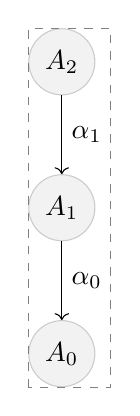
\begin{tikzpicture}[baseline=(X), bend angle=70, auto, fct/.style={circle, draw=gray!40, fill=gray!10}]
		\node[fct] (A0) {$A_0$};
		\node[fct] (A1) [above=of A0] {$A_1$} edge[->] node {$\alpha_0$} (A0);
		\node[fct] (A2) [above=of A1] {$A_2$} edge[->] node {$\alpha_1$} (A1);
		\coordinate (X) at (A1);
		\draw[dashed, gray] (current bounding box.south west) rectangle (current bounding box.north east);
	\end{tikzpicture} = 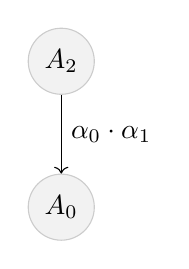
\begin{tikzpicture}[baseline=(X), bend angle=70, auto, fct/.style={circle, draw=gray!40, fill=gray!10}]
		\node[fct] (A0) {$A_0$};
		\node[fct] (A2) [above=of A0] {$A_2$} edge[->] node {$\alpha_0 \cdot \alpha_1$} (A0);
		\coordinate (X) at ($(A0)!.5!(A2)$);
	\end{tikzpicture} \quad \text{dan} \quad 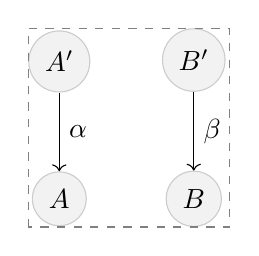
\begin{tikzpicture}[baseline=(X), bend angle=70, auto, fct/.style={circle, draw=gray!40, fill=gray!10}]
		\node[fct] (A) {$A$}; \node[fct] (A') [above=of A] {$A'$} edge[->] node {$\alpha$} (A);
		\node[fct] (B) [right=of A] {$B$}; \node[fct] (B') [above=of B] {$B'$} edge[->] node {$\beta$} (B);
		\coordinate (X) at ($(A)!.5!(A')$);
		\draw[dashed, gray] (current bounding box.south west) rectangle (current bounding box.north east);
	\end{tikzpicture} = 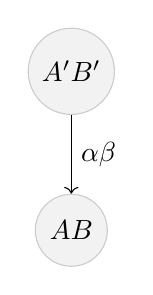
\begin{tikzpicture}[baseline=(X), bend angle=70, auto, fct/.style={circle, draw=gray!40, fill=gray!10}]
		\node[fct] (C) {$AB$};
		\node[fct] (D) [above=of C] {$A'B'$} edge[->] node {$\alpha\beta$} (C);
		\coordinate (X) at ($(C)!.5!(D)$);
	\end{tikzpicture} \]
	Lema \ref{prop:naturaltrans-associativity} setara dengan mengatakan bahwa ketika diagram dikomposisikan, kita boleh mendahulukan komposisi vertikal lalu horizontal, atau mendahulukan komposisi horizontal lalu vertikal. Sesuai konvensi, fungtor identitas tidak diberi label. Dengan demikian, $\eta, \varepsilon$ beserta invers masing-masing digambarkan sebagai berikut.
	\begin{center}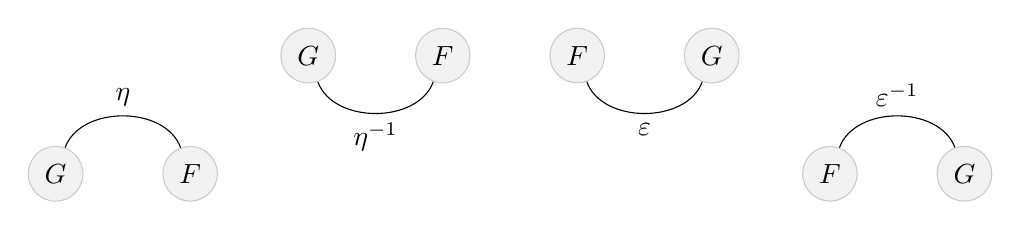
\begin{tikzpicture}[bend angle=70, auto, fct/.style={circle, draw=gray!40, fill=gray!10}]
		\node[fct] (G1) {$G$}; \node[fct] (F1) [right=of G1] {$F$} edge[bend right] node[swap] {$\eta$} (G1);
		\node[fct] (G2) [above right=of F1] {$G$}; \node[fct] (F2) [right=of G2] {$F$} edge[bend left] node {$\eta^{-1}$} (G2);
		\node[fct] (F3) [right=of F2] {$F$}; \node[fct] (G3) [right=of F3] {$G$} edge[bend left] node {$\varepsilon$} (F3);
		\node[fct] (F4) [below right=of G3] {$F$}; \node[fct] (G4) [right=of F4] {$G$} edge[bend right] node[swap] {$\varepsilon^{-1}$} (F4);
	\end{tikzpicture}\end{center}
	Untuk automorfisme identitas suatu fungtor, sisi yang bersesuaian tidak diberi nama. Sekarang kita nyatakan bahwa $\varepsilon': FG \to \identity$ memiliki dua representasi berikut:
	\begin{equation}\label{eqn:adj-equiv-two-expression} 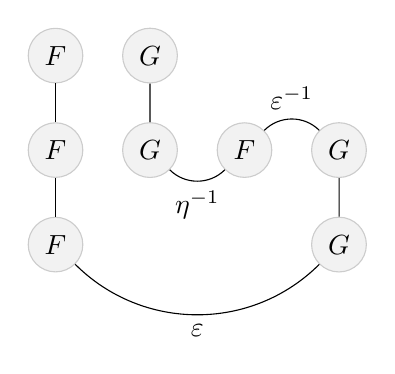
\begin{tikzpicture}[baseline=(X), scale=0.8, bend angle=45, auto, fct/.style={circle, draw=gray!40, fill=gray!10}, scale=1.5]
		\node[fct] (X0) at (0,1) {$F$};
		\node[fct] (X1) at (1,1) {$G$};

		\node[fct] (Y0) at (0,0) {$F$} edge (X0);
		\node[fct] (Y1) at (1,0) {$G$} edge (X1);
		\node[fct] (Y2) at (2,0) {$F$} edge[bend left] node {$\eta^{-1}$} (Y1);
		\node[fct] (Y3) at (3,0) {$G$} edge[bend right] node[swap] {$\varepsilon^{-1}$} (Y2);

		\node[fct] (Z0) at (0,-1) {$F$} edge (Y0);
		\node[fct] (Z1) at (3,-1) {$G$} edge (Y3) edge[bend left] node {$\varepsilon$} (Z0);
		\coordinate (X) at (0, -0.5);
	\end{tikzpicture} \quad = \quad 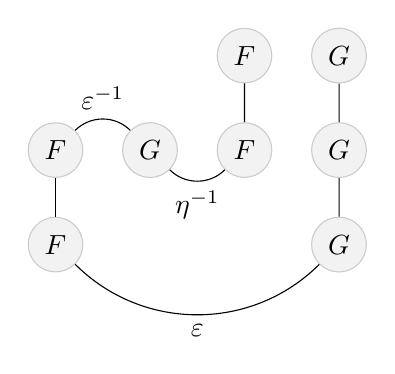
\begin{tikzpicture}[baseline=(X), scale=0.8, bend angle=45, auto, fct/.style={circle, draw=gray!40, fill=gray!10}, scale=1.5]
		\node[fct] (X0) at (2,1) {$F$};
		\node[fct] (X1) at (3,1) {$G$};

		\node[fct] (Y0) at (0,0) {$F$};
		\node[fct] (Y1) at (1,0) {$G$} edge[bend right] node[swap] {$\varepsilon^{-1}$} (Y0);
		\node[fct] (Y2) at (2,0) {$F$} edge[bend left] node {$\eta^{-1}$} (Y1) edge (X0);
		\node[fct] (Y3) at (3,0) {$G$} edge (X1);
	
		\node[fct] (Z0) at (0,-1) {$F$} edge (Y0);
		\node[fct] (Z1) at (3,-1) {$G$} edge (Y3) edge[bend left] node {$\varepsilon$} (Z0);
		\coordinate (X) at (0, -0.5);
	\end{tikzpicture} \end{equation}
	Diagram kiri memang merupakan penggambaran dari $\varepsilon \cdot (F\eta^{-1}G) \cdot (FG\varepsilon^{-1})$, sebab $FG\varepsilon^{-1}$ tidak lain ialah $\varepsilon^{-1}$ yang dikomposisikan secara horizontal di sebelah kiri oleh $\identity_F$ dan $\identity_G$, dan demikian seterusnya. Untuk beralih ke diagram kanan, gambarkan $FG \varepsilon^{-1}: FG \to FGFG$ sebagai berikut:
	\[ 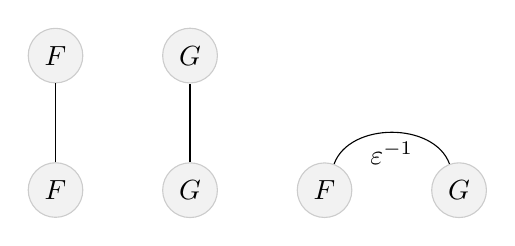
\begin{tikzpicture}[baseline=(X), bend angle=70, auto, fct/.style={circle, draw=gray!40, fill=gray!10}]
		\node[fct] (X0) {$F$}; \node[fct] (X1) [right=of X0] {$G$};
		\node[fct] (Y0) [below=of X0] {$F$} edge (X0); \node[fct] (Y1) [below=of X1] {$G$} edge (X1);
		\node[fct] (Y2) [right=of Y1] {$F$};
		\node[fct] (Y3) [right=of Y2] {$G$} edge[bend right] node {$\varepsilon^{-1}$} (Y2);
		\coordinate (X) at ($(X0)!.5!(Y0)$);
	\end{tikzpicture} = 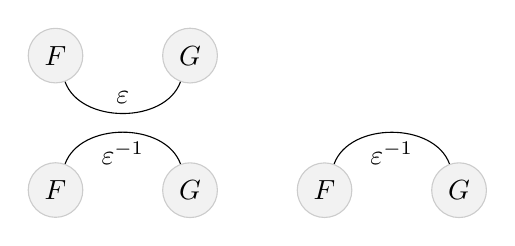
\begin{tikzpicture}[baseline=(X), bend angle=70, auto, fct/.style={circle, draw=gray!40, fill=gray!10}]
		\node[fct] (X0) {$F$}; \node[fct] (X1) [right=of X0] {$G$} edge[bend left] node[swap] {$\varepsilon$} (X0);
		\node[fct] (Y0) [below=of X0] {$F$}; \node[fct] (Y1) [below=of X1] {$G$} edge[bend right] node {$\varepsilon^{-1}$} (Y0);
		\node[fct] (Y2) [right=of Y1] {$F$};
		\node[fct] (Y3) [right=of Y2] {$G$} edge[bend right] node {$\varepsilon^{-1}$} (Y2);
		\coordinate (X) at ($(X0)!.5!(Y0)$);
	\end{tikzpicture} \]
	Karena komposisi horizontal dengan fungtor identitas tidak menimbulkan perubahan, $\varepsilon$ pada lapisan atas dapat ditempatkan di sebelah kiri ataupun kanan. Dengan demikian, diagram kanan menyederhana menjadi
	\[ 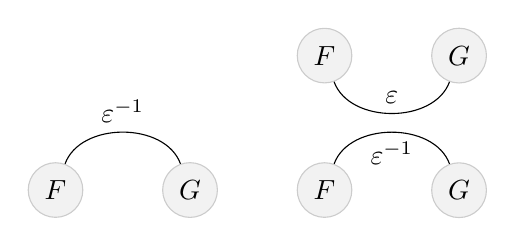
\begin{tikzpicture}[baseline=(X), bend angle=70, auto, fct/.style={circle, draw=gray!40, fill=gray!10}]
		\node[fct] (X0) {$F$}; \node[fct] (X1) [right=of X0] {$G$} edge[bend left] node[swap] {$\varepsilon$} (X0);
		\node[fct] (Y0) [below=of X0] {$F$}; \node[fct] (Y1) [below=of X1] {$G$} edge[bend right] node {$\varepsilon^{-1}$} (Y0);
		\node[fct] (Y3) [left=of Y0] {$G$};
		\node[fct] (Y2) [left=of Y3] {$F$} edge[bend left] node {$\varepsilon^{-1}$} (Y3);
		\coordinate (X) at ($(X0)!.5!(Y0)$);
	\end{tikzpicture} = 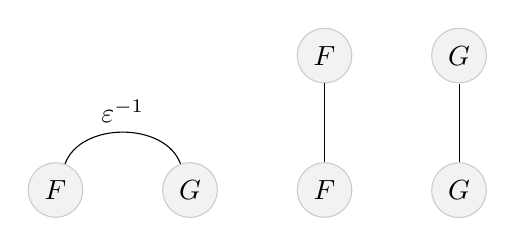
\begin{tikzpicture}[baseline=(X), bend angle=70, auto, fct/.style={circle, draw=gray!40, fill=gray!10}]
		\node[fct] (X0) {$F$}; \node[fct] (X1) [right=of X0] {$G$};
		\node[fct] (Y0) [below=of X0] {$F$} edge (X0); \node[fct] (Y1) [below=of X1] {$G$} edge (X1);
		\node[fct] (Y3) [left=of Y0] {$G$};
		\node[fct] (Y2) [left=of Y3] {$F$} edge[bend left] node {$\varepsilon^{-1}$} (Y3);
		\coordinate (X) at ($(X0)!.5!(Y0)$);
	\end{tikzpicture} \]
	Dengan menambahkan $\varepsilon \cdot (F\eta^{-1}G)$ di bawah ruas kanan, kita memperoleh \eqref{eqn:adj-equiv-two-expression}.

	Sekarang kita buktikan \eqref{eqn:adj-zigzag-2}. Substitusikan diagram kiri dalam \eqref{eqn:adj-equiv-two-expression} untuk $\varepsilon'$; dengan menghilangkan label fungtor, $(G\varepsilon')(\eta G)$ dapat digambarkan sebagai
	\[ 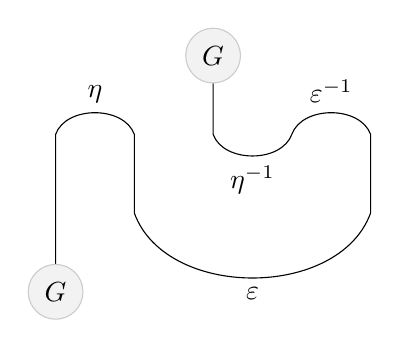
\begin{tikzpicture}[baseline=(X), bend angle=70, auto, fct/.style={circle, draw=gray!40, fill=gray!10}]
		\coordinate (A) at (0,0); \coordinate (B) at (0,2); \coordinate (C) at (1,2); \coordinate (D) at (1,1); \coordinate (E) at (4,1); \coordinate (F) at (4,2); \coordinate (G) at (3,2); \coordinate (H) at (2,2); \coordinate (I) at (2,3);
	
		\draw (A) -- (B) to[bend left] node {$\eta$} (C) -- (D) to[bend right] node[swap] {$\varepsilon$} (E) -- (F) to[bend right] node[swap] {$\varepsilon^{-1}$} (G) to[bend left] node {$\eta^{-1}$} (H) -- (I);
	
		\node[fct] at (A) {$G$}; \node[fct] at (I) {$G$};
		\coordinate (X) at (0, 1.5);
	\end{tikzpicture} \quad = \quad
	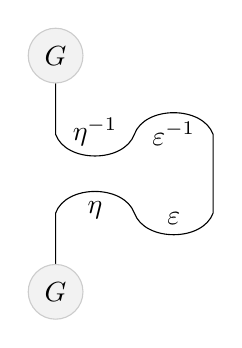
\begin{tikzpicture}[baseline=(X), bend angle=70, auto, fct/.style={circle, draw=gray!40, fill=gray!10}]
		\coordinate (A) at (0,0); \coordinate (B) at (0,1); \coordinate (C) at (1,1); \coordinate (D) at (2,1); \coordinate (E) at (2,2); \coordinate (F) at (1,2); \coordinate (G) at (0,2); \coordinate (H) at (0,3);
	
		\draw (A) -- (B) to[bend left] node[swap] {$\eta$} (C) to[bend right] node {$\varepsilon$} (D) -- (E) to[bend right] node {$\varepsilon^{-1}$} (F) to [bend left] node[swap] {$\eta^{-1}$} (G) -- (H);
		\node[fct] at (A) {$G$}; \node[fct] at (H) {$G$};
		\coordinate (X) at (0, 1.5);
	\end{tikzpicture}\]
	Untuk mengubah diagram kiri menjadi diagram kanan, mula-mula rentangkan diagram itu secara vertikal (yakni, sisipkan $\identity_F$, $\identity_G$, dan seterusnya di tengah), kemudian geser $\eta^{-1}$ ke kiri; alasannya serupa dengan argumen bagi \eqref{eqn:adj-equiv-two-expression}. Sekarang, dengan menggunakan $\eta \eta^{-1} = \identity_{GF}$ dan $\varepsilon^{-1}\varepsilon = \identity$, diagram kanan dapat disederhanakan menjadi
	\[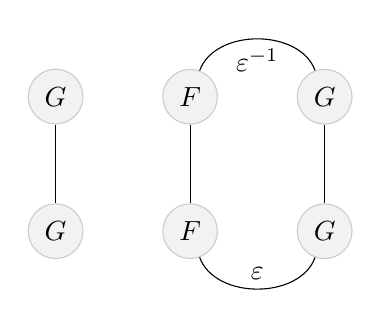
\begin{tikzpicture}[baseline=(X), bend angle=70, auto, fct/.style={circle, draw=gray!40, fill=gray!10}]
		\node[fct] (A) {$G$}; \node[fct] (B) [above=of A] {$G$} edge (A);
		\node[fct] (C) [right=of A] {$F$}; \node[fct] (D) [above=of C] {$F$} edge (C);
		\node[fct] (E) [right=of C] {$G$} edge[bend left] node[swap] {$\varepsilon$} (C);
		\node[fct] (F) [right=of D] {$G$} edge[bend right] node {$\varepsilon^{-1}$} (D) edge (E);
		\coordinate (X) at ($(A)!.5!(B)$);
	\end{tikzpicture} \quad = \quad 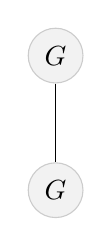
\begin{tikzpicture}[baseline=(X), bend angle=70, auto, fct/.style={circle, draw=gray!40, fill=gray!10}]
		\node[fct] (A) {$G$}; \node[fct] (B) [above=of A] {$G$} edge (A);
		\coordinate (X) at ($(A)!.5!(B)$);
	\end{tikzpicture}\]
	Ini membuktikan \eqref{eqn:adj-zigzag-2}. Kasus \eqref{eqn:adj-zigzag-1} hampir merupakan bayangan cermin dari argumen di atas; satu-satunya perbedaan ialah kita menggunakan diagram kanan dalam \eqref{eqn:adj-equiv-two-expression} untuk menggantikan $\varepsilon'$.
	
		Terakhir, kita buktikan keunikannya. Andaikan $\varepsilon'': FG \to \identity$ juga memenuhi \eqref{eqn:adj-zigzag-1} dan \eqref{eqn:adj-zigzag-2}. Perhatikan bahwa $\varepsilon''\cdot (\varepsilon' FG) = \varepsilon' \cdot (FG \varepsilon'')$; hal ini karena keduanya bersesuaian dengan diagram yang sama, $FGFG \to \identity$:
	\[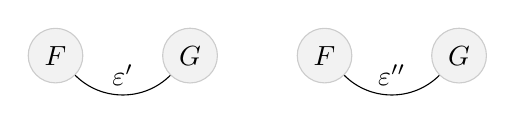
\begin{tikzpicture}[baseline=(X), bend angle=45, auto, fct/.style={circle, draw=gray!40, fill=gray!10}]
		\node[fct] (F) {$F$}; \node[fct] (G) [right=of F] {$G$} edge[bend left] node[swap] {$\varepsilon'$} (F);
		\node[fct] (F1) [right=of G] {$F$}; \node[fct] (G1) [right=of F1] {$G$} edge[bend left] node[swap] {$\varepsilon''$} (F1);
		\coordinate (X) at (F);
	\end{tikzpicture}.\]
	Selain itu, mudah dilihat bahwa $(\varepsilon'F \cdot F\eta)G = \varepsilon' FG \cdot F\eta G$ dan $F(G\varepsilon'' \cdot \eta G) = FG\varepsilon'' \cdot F\eta G$. Dengan menerapkan \eqref{eqn:adj-zigzag-1} dan \eqref{eqn:adj-zigzag-2}, keduanya sama dengan $\identity_{FG}$. Oleh karena itu, $\varepsilon'' = \varepsilon'' \cdot (\varepsilon' FG) (F\eta G) = \varepsilon' (FG\varepsilon'')(F\eta G) = \varepsilon'$. Keunikan pun terbukti.
\end{proof}

Dalam teori kategori masih terdapat banyak teknik visualisasi serupa. Pembaca dapat merujuk kepada survei yang ditulis P.\ Selinger dalam \cite[Chapter 4]{Co11}. Teknik serupa akan kita jumpai lagi dalam \S\ref{sec:braiding}.
	
\section{Limit}\label{sec:limits}
Pertama-tama kita berikan definisi umum limit, lalu menguraikannya secara bertahap.

\begin{definition}\label{def:diagonal-functor}
	Misalkan $I, \mathcal{C}$ kategori. Definisikan fungtor diagonal $\Delta: \mathcal{C} \to \mathcal{C}^I := \text{Fct}(I, \mathcal{C})$ sebagai berikut: fungtor ini memetakan setiap $X \in \Obj(\mathcal{C})$ ke fungtor konstan
	\begin{gather*}
		\Delta(X): I \longrightarrow \mathcal{C}\;
		\left\{ \begin{array}{ll}
			\forall i \in \Obj(I), & i \longmapsto X \\
			\forall [i \to j] \in \Mor(I), & [i \to j] \longmapsto [\identity_X: X \to X].
		\end{array}\right.
	\end{gather*}
	Untuk morfisme $f: X \to Y$ yang diberikan, dalam kategori $\mathcal{C}^I$ definisi $\Delta(f): \Delta(X) \to \Delta(Y)$ sudah jelas: pada setiap $i \in \Obj(I)$, komponennya adalah $f: X \to Y$.
\end{definition}

Dengan memakai $I^{\text{op}}$ sebagai pengganti $I$, dapat pula didefinisikan fungtor diagonal $\Delta: \mathcal{C} \to \mathcal{C}^{I^{\text{op}}} := \text{Fct}(I^{\text{op}}, \mathcal{C})$. Ingat Definisi \ref{def:comma-category} dan pembahasan sesudahnya: untuk fungtor $I \xrightarrow{\alpha} \mathcal{C} \xleftarrow{\beta} I^\text{op}$, dapat dibentuk dua kategori koma
\begin{align*}
	\left[ \mathbf{1} \xrightarrow{j_\alpha} \mathcal{C}^I \xleftarrow{\Delta} \mathcal{C} \right] & \leadsto \quad (j_\alpha/\Delta) =: (\alpha / \Delta), \\
	\left[ \mathcal{C} \xrightarrow{\Delta} \mathcal{C}^{I^\text{op}} \xleftarrow{j_\beta} \mathbf{1} \right] & \leadsto \quad (\Delta/j_\beta) =: (\Delta/\beta).
\end{align*}
\begin{definition}[Limit]\label{def:limit}\index{guinajixian@limit induktif (inductive limit)}\index{toushejixian@limit proyektif (projective limit)}\index[sym1]{limind@$\varinjlim$}\index[sym1]{limproj@$\varprojlim$}
	Misalkan $I, \mathcal{C}$ kategori. Pertimbangkan fungtor $\alpha: I \to \mathcal{C}$ dan $\beta: I^\text{op} \to \mathcal{C}$.
	\begin{compactenum}
		\item Jika kategori koma $(\alpha / \Delta)$ mempunyai objek awal, objek itu dinotasikan dengan $\varinjlim \alpha$ dan disebut \emph{limit induktif} dari $\alpha$;
		\item Jika kategori koma $(\Delta / \beta)$ mempunyai objek terminal, objek itu dinotasikan dengan $\varprojlim \beta$ dan disebut \emph{limit proyektif} dari $\beta$.
	\end{compactenum}
	Keduanya juga disebut limit berindeks $I$.
\end{definition}
Terminologi tentang limit belum seragam; berikut beberapa versi yang lazim.
\begin{center}\begin{tabular}{c|c}
	$\varinjlim$ & $\varprojlim$ \\
	Limit induktif & Limit proyektif \\
	Limit langsung & Limit invers \\
	Kolimit ($\text{colim}$) & Limit ($\text{lim}$)
\end{tabular}\end{center}

Proposisi \ref{prop:initial-obj-uniqueness} menjamin bahwa setiap limit, jika ada, bersifat unik. Lebih tepatnya, kategori koma memberikan deskripsi berikut berdasarkan diagram komutatif dalam $\mathcal{C}$
\begin{equation*}\begin{gathered}
	(\alpha/\Delta): \left\{ \begin{array}{ll}
		\text{objek}: & \left( L, (\alpha(i) \xrightarrow{f_i} L)_{i \in \Obj(I)} \right), \quad \forall\; [i \xrightarrow{\phi} j], \;
			\begin{tikzcd}[column sep=tiny, row sep=tiny]
				\alpha(i) \arrow[rd] \arrow[rr, "{\alpha(\phi)}"] & & \alpha(j) \arrow[ld] \\
				{} & L &
			\end{tikzcd} \\
		\text{morfisme}: & \left[ \varphi: (L, (f_i)_i) \to (L', (f'_i)_i) \right] =  \forall i, \;
			\begin{tikzcd}[column sep=tiny, row sep=small]
				\alpha(i) \arrow[r, "f_i"] \arrow[rd, "f'_i"'] & L \arrow[d, "\varphi"] \\
				{} & L'
			\end{tikzcd}
	\end{array}\right. \\
	(\Delta/\beta): \left\{ \begin{array}{ll}
		\text{objek}: & \left( L, (L \xrightarrow{g_i} \beta(i))_{i \in \Obj(I)} \right), \quad \forall\; [i \xrightarrow{\phi} j], \;
			\begin{tikzcd}[column sep=tiny, row sep=tiny]
				\beta(i) & & \beta(j) \arrow[ll, "\beta(\phi)"'] \\
				{} & L \arrow[lu] \arrow[ru] &
			\end{tikzcd} \\
		\text{morfisme}: & \left[ \varphi: (L, (g_i)_i) \to (L', (g'_i)_i) \right] =  \forall i, \;
			\begin{tikzcd}[column sep=tiny, row sep=small]
				\beta(i) & L \arrow[d, "\varphi"] \arrow[l, "g_i"'] \\
				{} & L' \arrow[lu, "g'_i"]
			\end{tikzcd}
	\end{array}\right.
\end{gathered}\end{equation*}

Dalam beberapa pustaka, objek dari $(\alpha/\Delta)$ dan $(\Delta/\beta)$ masing-masing disebut kerucut dan kokerucut; sebutan ini bersifat intuitif.

Dengan demikian, limit induktif dari $\alpha$ dapat dipahami kembali sebagai data $(\varinjlim \alpha, \alpha(i) \xrightarrow{\iota_i} \varinjlim \alpha)$, sedangkan limit proyektif dari $\beta$ sebagai data $(\varprojlim \beta, \varprojlim \beta \xrightarrow{p_i} \beta(i))$; sifat universal masing-masing digambarkan oleh
\begin{equation}\label{eqn:lim-diagrams}\begin{tikzcd}
	\alpha(i) \arrow[rd, "{\iota_i}"] \arrow[rdd] \arrow[rr, "{\alpha(\phi)}"] & & \alpha(j) \arrow[ld, "{\iota_j}"'] \arrow[ldd] \\
	& \varinjlim \alpha \arrow[dashed, d, "\exists !"] &  \\
	& L &
	\end{tikzcd}\quad\begin{tikzcd}
	\beta(i) & & \beta(j) \arrow[ll, "{\beta(\phi)}"'] \\
	& \varprojlim \beta \arrow[lu, "p_i"'] \arrow[ru, "p_j"] & \\
	& L \arrow[luu] \arrow[ruu] \arrow[dashed, u, "{\exists !}"'] &
\end{tikzcd}\end{equation}
Diagram tersebut dibaca sebagai berikut: untuk setiap objek dari $(\alpha / \Delta)$ atau $(\Delta/\beta)$ yang berbentuk $(L, \ldots)$, terdapat morfisme tunggal $\dashrightarrow$ sehingga seluruh diagram komutatif untuk setiap $\phi \in \Mor(I)$.

\begin{remark}\label{rem:lim-duality}
	Perhatikan bahwa arah panah pada kedua diagram dalam \eqref{eqn:lim-diagrams} saling berlawanan. Sesungguhnya, $\varinjlim$ dan $\varprojlim$ adalah konsep dual: misalkan $\alpha: I \to \mathcal{C}$; pada kategori lawan terdapat $\alpha^\text{op}: I^\text{op} \to \mathcal{C}^\text{op}$ yang bersesuaian (Catatan \ref{rem:op-functor}). Untuk $I^\text{op}$ dan $\mathcal{C}^\text{op}$ terdapat pula fungtor diagonal $\Delta^{\text{op}}$ yang bersesuaian. Dengan demikian diperoleh
	\begin{align*}
		(\alpha / \Delta)^\text{op} & = (\Delta^\text{op} / \alpha^\text{op}), \\
		\varprojlim (\alpha^{\text{op}}) & = \varinjlim \alpha, \quad \text{jika limit pada salah satu ruas ada}.
	\end{align*}
\end{remark}

\begin{lemma}\label{prop:lim-functoriality}
	Misalkan $\psi: \alpha \to \alpha'$ suatu morfisme dalam kategori fungtor $\mathcal{C}^I$. Andaikan semua $\varinjlim$ yang bersesuaian ada. Maka terdapat morfisme tunggal $\varinjlim \psi$ sedemikian sehingga
	\begin{tikzcd}[row sep=small, column sep=small]
		\alpha(i) \arrow[r] \arrow[d, "\psi(i)"'] & \varinjlim \alpha \arrow[d, "\varinjlim\psi"] \\
		\alpha'(i) \arrow[r] & \varinjlim \alpha'
	\end{tikzcd}
	komutatif untuk setiap $i$. Jika $\alpha \xrightarrow{\psi_1} \alpha' \xrightarrow{\psi_2} \alpha''$, maka $\varinjlim (\psi_2 \psi_1) = \varinjlim \psi_2 \varinjlim \psi_1$. Hasil serupa juga berlaku untuk $\varprojlim$: secara natural, $\psi: \beta \to \beta'$ menginduksi $\varprojlim \beta \to \varprojlim \beta'$, dan seterusnya.
\end{lemma}
\begin{proof}
	Dalam sifat universal $\varinjlim \alpha$, cukup ambil $L := \varinjlim \alpha' \leftarrow \alpha'(i) \xleftarrow{\psi(i)} \alpha(i)$. Sifat $\varinjlim (\psi_2 \psi_1) = \varinjlim \psi_2 \varinjlim \psi_1$ mengikuti dari
	\[\begin{tikzcd}[row sep=small, column sep=small]
		\alpha(i) \arrow[r] \arrow[d] & \alpha'(i) \arrow[r] \arrow[d] & \alpha''(i) \arrow[d] \\
		\varinjlim \alpha \arrow[r] & \varinjlim \alpha' \arrow[r] & \varinjlim \alpha''
	\end{tikzcd} \qquad i \in \Obj(I) \]
	komutativitas seluruh diagram.
\end{proof}

Selanjutnya kita mengikuti Konvensi \ref{con:U-small} dan membedakan kategori dari kategori kecil. Kita hanya mempertimbangkan limit dengan $I$ kategori kecil. Hal ini terutama demi kemudahan perumusan; lagi pula, menurut Hipotesis \ref{hyp:universe}, semesta $\mathcal{U}$ yang dipilih selalu dapat diperbesar agar semua kategori yang dibahas menjadi kategori kecil. Namun, pembaca tetap perlu waspada karena dalam beberapa situasi ukuran himpunan benar-benar dapat menimbulkan perbedaan substantif, seperti dalam Proposisi \ref{prop:preorder-complete} yang akan disebutkan di bawah.

\begin{example}\label{eg:set-limits}
	Ambil $\mathcal{C} := \cate{Set}$ dan misalkan $I$ kategori kecil. Pertama-tama kita konstruksikan $\varprojlim \beta$. Definisikan
	\begin{align*}
		\varprojlim \beta & := \left\{ (x_i)_{i \in \Obj(I)} \in \prod_i \beta(i) : \forall \sigma \in \Hom_I(i,j), \; \beta(\sigma)(x_j) = x_i \right\} \\
		& = \Ker\left[ \prod_i \beta(i) \rightrightarrows \prod_\sigma \beta(s(\sigma)) \right] \quad \text{(ekualiser)},
	\end{align*}
	Kedua panah dalam $\Ker[\cdots]$ masing-masing memiliki pemetaan $(x_i)_i \mapsto x_{s(\sigma)}$ dan $(x_i)_i \mapsto \beta(\sigma)\left(x_{t(\sigma)}\right)$ sebagai ``koordinat-$\sigma$''-nya, dengan $\sigma$ merentang semua morfisme dalam $I$. Ekspresi di atas merupakan sebuah objek dalam $\cate{Set}$ dan dilengkapi keluarga pemetaan proyeksi $p_j: \varprojlim \beta \to \beta(j)$, $p_j((x_i)_i) = x_j$, dengan $j$ merentang $\Obj(I)$. Tidak sulit memeriksa bahwa $(\varprojlim \beta, (p_j)_j)$ adalah limit proyektif dari $\beta$.

	Selanjutnya, pertimbangkan $\alpha: I \to \cate{Set}$. Definisikan
	\[ \varinjlim \alpha := \left( \bigsqcup_{i \in \Obj(I)} \alpha(i) \right) \Big/ \sim \]
	dengan $\bigsqcup_i \alpha(i)$ menyatakan gabungan saling lepas, sedangkan $\sim$ adalah relasi ekuivalensi yang dibangkitkan oleh relasi berikut
	\[ x \sim \alpha(\sigma)(x), \quad \sigma: i \to j, \quad x \in \alpha(i). \]
	Dari sifat himpunan hasil bagi diperoleh keluarga pemetaan $\iota_j: \alpha(j) \to \varinjlim \alpha$, dengan $j$ merentang $\Obj(I)$; pemetaan ini membawa $x \in \alpha(j)$ ke kelas ekuivalensi yang memuat $x$. Tidak sulit memeriksa bahwa $(\varinjlim \alpha, (\iota_j)_j)$ adalah limit induktif dari $\alpha$.
\end{example}
Konstruksi di atas memiliki satu kekurangan yang jelas: konstruksi itu hanya menjelaskan cara ``membangkitkan'' relasi ekuivalensi $\sim$, tetapi tidak memberikan deskripsi langsung. Untuk mengatasinya, diperlukan syarat tambahan pada $I$; pada saat yang sama kita perkenalkan konsep kategori terarah ke atas.

\begin{definition}\label{def:filtrant-cat}\index{luguofanchou@kategori terarah ke atas (filtered category)}
	Kategori tak kosong $I$ disebut \emph{terarah ke atas (filtered)} jika memenuhi syarat-syarat berikut:
	\begin{compactitem}
		\item Untuk setiap $i, j \in \Obj(I)$, terdapat $k \in \Obj(I)$ dan morfisme $i \to k$, $j \to k$;
		\item Untuk setiap panah $f,g: i \to j$, terdapat $k \in \Obj(I)$ dan $h: j \to k$ sedemikian sehingga $hf = hg$.
	\end{compactitem}
\end{definition}
Untuk kategori yang berasal dari poset tak kosong $(I, \leq)$, syarat kedua bersifat mubazir; dalam hal ini kita kembali pada konsep poset terarah ke atas (filtered poset) yang didefinisikan dalam \S\ref{sec:group-limit}. Sebagai contoh, poset $(\Z_{\geq 1}, \leq)$ adalah poset terarah ke atas.

Sekarang kembali ke Contoh \ref{eg:set-limits}, yakni fungtor $\alpha: I \to \cate{Set}$, dan andaikan $I$ terarah ke atas. Pada gabungan saling lepas $\bigsqcup_{i \in \Obj(I)} \alpha(i)$, definisikan relasi $\sim$ sebagai berikut: untuk setiap $i, j \in \Obj(I)$ serta $x_i \in \alpha(i)$, $x_j \in \alpha(j)$, jika
\begin{equation}\label{eqn:filtrant-equiv} \text{terdapat} \begin{cases}
	f: i \to k, \\
	g: j \to k
	\end{cases}
	\text{sedemikian sehingga} \quad \alpha(f)(x_i) = \alpha(g)(x_j) \in \alpha(k)
\end{equation}
maka tetapkan $x_i \sim x_j$. Jelas bahwa relasi ekuivalensi dalam Contoh \ref{eg:set-limits} juga harus memenuhi sifat ini. Jika dapat ditunjukkan bahwa $\sim$ sudah merupakan relasi ekuivalensi, maka $\sim$ di sini tepat sama dengan relasi dalam Contoh \ref{eg:set-limits} yang juga dinotasikan $\sim$. Refleksivitas dan simetrinya jelas; kini kita periksa transitivitasnya. Andaikan $(x_i \sim x_j) \wedge (x_j \sim x_k)$; terdapat diagram
\[ \begin{tikzcd}[scale=0.75]
	i \arrow[rd] & & j \arrow[ld] \arrow[rd] & & k \arrow[ld] \\
	& h \arrow[dashed, rd] & & h' \arrow[dashed, ld] & \\
	& & g & &
\end{tikzcd} \quad \begin{tikzcd}[scale=0.75]
	x_i \arrow[mapsto, rd] & & x_j \arrow[mapsto, ld] \arrow[mapsto, rd] & & x_k \arrow[mapsto, ld] \\
	& x_h \arrow[dashed, rd] & & x_{h'} \arrow[dashed, mapsto, ld] & \\
	& & ? & & 
\end{tikzcd} \]
Panah putus-putus dan $g$ di dalamnya dilengkapi dengan syarat pertama Definisi \ref{def:filtrant-cat}. Akan tetapi, citra $x_h$ dan $x_{h'}$ di bawah panah putus-putus belum tentu sama. Karena itu, dengan syarat kedua definisi tersebut, kita cari dalam $I$ suatu morfisme $g \to g'$ sehingga morfisme komposit $j \to h \to g \to g'$ sama dengan $j \to h' \to g \to g'$. Dengan memakai $g'$ sebagai pengganti $g$ dalam diagram, dapat dipastikan bahwa $x_i \sim x_k$. Jadi, $\sim$ merupakan relasi ekuivalensi. Dari definisi $\sim$ juga diperoleh komutativitas diagram kiri dalam \eqref{eqn:lim-diagrams}. Ringkasnya,
\[ \varinjlim \alpha := \bigsqcup_{i \in \Obj(I)} \alpha(i) \big/ \sim \]
Kelak kita akan berulang kali mempertimbangkan $\varinjlim$ berindeks kategori terarah ke atas dalam berbagai kategori.

\begin{example}\label{eg:top-limits}
	Dengan cara yang sama dapat dikonstruksikan limit dalam kategori $\mathcal{C} := \cate{Top}$. Untuk kategori kecil $I$, konstruksi limit $(\varinjlim \alpha, \iota_j)$ dan $(\varprojlim \beta, p_j)$ persis sama dengan konstruksi dalam $\cate{Set}$; kita hanya perlu melengkapi himpunan-himpunan tersebut dengan topologi hasil bagi atau topologi subruang \cite[\S 3.1, \S 3.4]{Xiong}.
\end{example}

Misalkan kategori $\mathcal{C}$ diberikan. Meskipun limit yang dibahas belum tentu ada dalam $\mathcal{C}$, setelah $\mathcal{C}$ dibenamkan ke kategori fungtor $\mathcal{C}^\wedge$ atau $\mathcal{C}^\vee$ (lihat \S\ref{sec:representable-functors}), keberadaan semua limit (kecil) dapat dijamin.

\begin{proposition}\label{prop:lim-Yoneda}
	Misalkan $I$ kategori kecil. Limit fungtor $\alpha: I \to \mathcal{C}^\wedge$ diberikan oleh objek $\Yinjlim \alpha \in \Obj(\mathcal{C}^\wedge)$ yang didefinisikan sebagai berikut:
	\begin{gather*}
		\Yinjlim \alpha: S \longmapsto \varinjlim \left( \alpha(S) \right), \\
		[T \xrightarrow{f} S] \leadsto \varinjlim \alpha(S) \xrightarrow{\varinjlim \alpha(f)} \varinjlim \alpha(T),
	\end{gather*}
	beserta keluarga transformasi natural $\alpha(j)(\cdot) \to \varinjlim \alpha(\cdot)$, dengan $j \in \Obj(I)$ dan konstruksi $\varinjlim \alpha(f)$ diberikan dalam Lema \ref{prop:lim-functoriality}; di sini $\varinjlim$ tanpa hiasan tambahan adalah limit dalam $\cate{Set}$. Demikian pula, limit fungtor $\beta: I^\text{op} \to \mathcal{C}^\wedge$ diberikan oleh
	\[ \Yprojlim \beta: S \longmapsto \varprojlim \left( \beta(S) \right) \]
	dan data-data serupa. Sifat serupa juga berlaku bagi kasus dengan nilai dalam $\mathcal{C}^\vee$; secara notasi, semua limit ini kita tulis tanpa membedakannya sebagai
	\begin{align*}
		\Yinjlim \alpha: S & \longmapsto \varinjlim \left( \alpha(S) \right), \quad \alpha: I \to \mathcal{C}^\wedge \;\text{atau}\; \mathcal{C}^\vee, \\
		\Yprojlim \beta: S & \longmapsto \varprojlim \left( \beta(S) \right), \quad \beta: I^\text{op} \to \mathcal{C}^\wedge \;\text{atau}\; \mathcal{C}^\vee.
	\end{align*}
\end{proposition}
\begin{proof}
	Caranya ialah mengambil limit fungtor secara titik demi titik (atau objek demi objek), sehingga kasusnya tereduksi ke $\cate{Set}$. Kita hanya uraikan kasus $\alpha: I \to \mathcal{C}^\wedge$ dan $\Yinjlim \alpha$. Pertimbangkan diagram \eqref{eqn:lim-diagrams} yang bersesuaian, serta berikan $L \in \mathcal{C}^\wedge$ dan keluarga morfisme $\alpha(i) \to L$. Untuk setiap $S \in \Obj(\mathcal{C})$, konstruksi dalam $\cate{Set}$ bagi $\varinjlim$ menunjukkan bahwa terdapat $\varphi(S)$ tunggal sehingga diagram
	\begin{tikzcd}[column sep=tiny, row sep=tiny]
		\alpha(i)(S) \arrow[rr] \arrow[rd] & & \varinjlim \alpha(S) \arrow[ld, "\varphi(S)"] \\
		& L(S) &
	\end{tikzcd}
	komutatif untuk semua $i$. Kuncinya ialah membuktikan bahwa semua $\varphi(\cdot)$ ini dapat, dalam $\mathcal{C}^\wedge$, dirangkai menjadi $\Yinjlim \alpha \xrightarrow{\varphi} L$. Pertimbangkan dalam $\mathcal{C}$ sebarang morfisme $f: T \to S$. Selanjutnya, pandang $L(S)$ sebagai fungtor konstan $\Delta(L(S)): I \to \cate{Set}$; mudah dilihat bahwa $\varinjlim$-nya adalah $L(S)$ sendiri (silakan periksa). Demikian pula untuk $L(T)$. Maka, dari Lema \ref{prop:lim-functoriality} diperoleh: untuk setiap $i \in \Obj(I)$,
	\[ \begin{tikzcd}
		\alpha(i)(S) \arrow[r, "\alpha(i)(f)"] \arrow[d] & \alpha(i)(T) \arrow[d] \\
		L(S) \arrow[r, "L(f)"'] & L(T)
	\end{tikzcd} \;\text{komutatif, sehingga} \;
	\begin{tikzcd}
		\varinjlim \alpha(S) \arrow[r, "{\varinjlim \alpha(f)}", yshift=0.5em] \arrow[d, "\varphi(S)"'] & \varinjlim \alpha(T) \arrow[d, "\varphi(T)"] \\
		L(S) \arrow[r, "L(f)"'] & L(T)
	\end{tikzcd} \;\text{komutatif}, \]
	dan diagram kanan tepat menyatakan fungtorialitas yang diperlukan oleh $\varphi(\cdot)$.
\end{proof}
Dengan demikian, keberadaan limit tereduksi pada representabilitas fungtor; lihat \S\ref{sec:representable-functors}.

\begin{proposition}\label{prop:lim-as-fct}
	Misalkan $I$ kategori kecil. Berikut ini kita menggunakan fungtor $k_{\mathcal{C}}$ dan $h_{\mathcal{C}}$ untuk memandang $\mathcal{C}$ masing-masing sebagai subkategori dari $\mathcal{C}^\vee$ dan $\mathcal{C}^\wedge$.
	\begin{enumerate}
		\item Limit induktif fungtor $\alpha: I \to \mathcal{C}$ ada jika dan hanya jika $\Yinjlim \alpha \in \mathcal{C}^\vee$ representabel; memberikan limit dari $\alpha$ ekuivalen dengan memberikan objek $\varinjlim \alpha \in \Obj(\mathcal{C})$ beserta isomorfisme $k_{\mathcal{C}}(\varinjlim \alpha) \rightiso \Yinjlim \alpha$.
		\item Limit proyektif fungtor $\beta: I^\text{op} \to \mathcal{C}$ ada jika dan hanya jika $\Yprojlim \beta \in \mathcal{C}^\wedge$ representabel; memberikan limit dari $\beta$ ekuivalen dengan memberikan objek $\varprojlim \beta \in \Obj(\mathcal{C})$ beserta isomorfisme $h_{\mathcal{C}}(\varprojlim \beta) \rightiso \Yprojlim \beta$.
	\end{enumerate}
\end{proposition}
Sifat limit dengan demikian dapat dicirikan secara ringkas sebagai
\begin{align*}
	\Hom_{\mathcal{C}}(\varinjlim \alpha, \cdot) & \rightiso \varprojlim_i \Hom_{\mathcal{C}}(\alpha(i), \cdot) = \Yinjlim \alpha, \\
	\Hom_{\mathcal{C}}(\cdot, \varprojlim \beta) & \rightiso \varprojlim_i \Hom_{\mathcal{C}}(\cdot, \beta(i)) = \Yprojlim \beta.
\end{align*}
Perhatikan bahwa $\mathcal{C}^\vee$ dan $\mathcal{C}^\wedge$ di sini tidak dapat dipertukarkan: limit di luar $\Hom_{\mathcal{C}}$ haruslah $\varprojlim$!

\begin{proof}
	Pertama, tinjau kasus limit induktif. Sifat universal dalam \eqref{eqn:lim-diagrams} dapat ditulis ulang sebagai berikut: memberikan limit dari $\alpha$ ekuivalen dengan memberikan objek $\varinjlim \alpha \in \Obj(\mathcal{C})$ beserta keluarga morfisme $\iota_i: \alpha(i) \to \varinjlim \alpha$, sedemikian sehingga morfisme antarfungtor
	\begin{equation*}\begin{tikzcd}[row sep=small]
		k_{\mathcal{C}}(\varinjlim \alpha) \arrow[equal, r] & \Hom_{\mathcal{C}}(\varinjlim \alpha , \cdot) \arrow[r, "\xi"] & \varprojlim_i \Hom_{\mathcal{C}}(\alpha(i), \cdot) & \Yinjlim \alpha \arrow[equal, l] \\
		& f \arrow[phantom, u, sloped, "\in" description] \arrow[mapsto, r] & (\iota_i^* f = f \circ \iota_i)_{i \in \Obj(I)} \arrow[phantom, u, sloped, "\in" description] &
	\end{tikzcd}\end{equation*}
	merupakan isomorfisme. Sebaliknya, setiap isomorfisme $\xi: k_{\mathcal{C}}(\varinjlim \alpha) \rightiso \Yinjlim \alpha$ dapat diinduksi dengan cara tersebut oleh suatu keluarga $\iota_i: \alpha(i) \to \varinjlim \alpha$: ini merupakan penerapan Teorema \ref{prop:Yoneda-lemma}. Secara lebih langsung, ambil peubah pada diagram di atas sebagai $\varinjlim \alpha$; citra dari $f = \identity$ tepat merupakan $(\iota_i)_i$ yang dicari.

	Kasus limit proyektif ditangani dengan cara yang sepenuhnya serupa; kali ini isomorfisme yang ditinjau ialah
	\begin{equation*}\begin{tikzcd}[row sep=small]
		\Hom_{\mathcal{C}}(\cdot, \varprojlim \beta) \arrow[r] & \varprojlim_i \Hom_{\mathcal{C}}(\cdot, \beta(i)) = \Yprojlim \beta \\
		f \arrow[phantom, u, sloped, "\in" description] \arrow[mapsto, r] & (p_{i *} f = p_i \circ f)_{i \in \Obj(I)} \arrow[phantom, u, sloped, "\in" description]
	\end{tikzcd}\end{equation*}
	Pernyataan pun terbukti.
\end{proof}

Proposisi \ref{prop:lim-as-fct} mereduksi banyak sifat limit ke kasus himpunan, sehingga pembuktiannya sangat disederhanakan. Mari kita lihat sebuah contoh.
\begin{lemma}\label{prop:lim-Fubini}
	Misalkan $I, J$ kategori kecil dan andaikan $\mathcal{C}$ memiliki limit induktif berindeks $I$ dan $J$, yang dinotasikan dengan $\varinjlim$. Pertimbangkan fungtor $\alpha: I \times J \to \mathcal{C}$. Terdapat isomorfisme kanonik
	\[ \varinjlim_j \left( \varinjlim\alpha(\cdot, j) \right) \simeq \varinjlim \alpha \simeq \varinjlim_i \left( \varinjlim\alpha(i, \cdot) \right) \]
	dengan limit pada ruas kiri diambil terlebih dahulu terhadap $I$, lalu terhadap $J$, sedangkan pada ruas kanan urutannya dibalik. Kasus limit proyektif $\varprojlim \beta$ serupa.
\end{lemma}
\begin{proof}
	Cukup buktikan kasus $\varinjlim$. Untuk suatu morfisme dalam $I$ yang diberikan, yakni $i \to i'$, Lema \ref{prop:lim-functoriality} memberikan diagram komutatif natural berikut untuk setiap $j$:
	\[ \begin{tikzcd}
		\varinjlim \alpha(i, \cdot) \arrow[r] & \varinjlim \alpha(i', \cdot) \\
		\alpha(i, j) \arrow[r] \arrow[u] & \alpha(i', j) \arrow[u]
	\end{tikzcd} \]
	Karena itu, limit pada ruas kanan dalam pernyataan tersebut terdefinisi; demikian pula ruas kiri. Proposisi \ref{prop:lim-as-fct} mereduksi pernyataan itu ke kategori $\mathcal{C} = \cate{Set}$, tepatnya kasus $\varprojlim$, yang langsung jelas dari konstruksi pada Contoh \ref{eg:set-limits}.
\end{proof}

Jika himpunan objek dan himpunan morfisme kategori $I$ keduanya berhingga, limit yang bersesuaian disebut limit berhingga; dalam hal ini, diagram lazim digunakan untuk mendeskripsikan konstruksi $I$. Limit dapat dikonstruksikan dalam dua tahap: produk (atau koproduk) dan ekualiser (atau koekualiser). Dalam pembahasan berikut, semua limit yang dibicarakan diandaikan ada.
\begin{asparaenum}\index{yuji@koproduk (coproduct)}\index{ji@produk (product)}
	\item Ambil $I$ sebagai kategori diskret; kita dapat mengidentifikasi $I$ dengan $\Obj(I)$. Dalam hal ini, $\varinjlim_{i \in I} \alpha(i)$ untuk objek-objek $X_i := \alpha(i)$ disebut \emph{koproduk} dan ditulis $\coprod_{i \in I} X_i$; sejalan dengan itu, $\prod_{i \in I} Y_i := \varprojlim_{i \in I} \beta(i)$ untuk objek-objek $Y_i := \beta(i)$ disebut \emph{produk}. Sifat universal \eqref{eqn:lim-diagrams} menjadi
		\[\begin{tikzcd}[row sep=small, column sep=small]
			\Hom_{\mathcal{C}} \left( \displaystyle\coprod_{i \in I} X_i, \cdot \right) \arrow[r, "\sim"] & \displaystyle\prod_{i \in I} \Hom_{\mathcal{C}}(X_i, \cdot) & \Hom_{\mathcal{C}} \left( \cdot, \displaystyle\prod_{i \in I} Y_i \right)  \arrow[r, "\sim"] & \displaystyle\prod_{i \in I} \Hom_{\mathcal{C}}(\cdot, Y_i) \\
			\phi \arrow[mapsto, r] & (\phi \iota_i)_{i \in I} & \phi \arrow[mapsto, r] & (p_i \phi)_{i \in I}
		\end{tikzcd}\]
		Di sini digunakan morfisme $\iota_j: X_j \to \coprod_i X_i$ dan $p_j: \prod_i Y_i \to Y_j$; yang terakhir disebut proyeksi ke $Y_j$.

		Koproduk atau produk dari sejumlah berhingga objek lazim ditulis $X_1 \sqcup \cdots \sqcup X_n$ atau $Y_1 \times \cdots \times Y_n$. Notasi ini sesuai dengan kelaziman dalam kasus $\cate{Set}$ dan $\cate{Top}$ (ruang produk, gabungan saling lepas).
	\item Ambil kategori kosong $I = \mathbf{0}$. Dalam hal ini, \eqref{eqn:lim-diagrams} menunjukkan bahwa $\varinjlim$ adalah objek awal, sedangkan $\varprojlim$ adalah objek terminal. Keduanya juga dapat dipahami masing-masing sebagai koproduk kosong dan produk kosong.
	\item Ambil $I$ sebagai kategori yang diberikan oleh diagram
		\begin{tikzcd}
			\bullet \arrow[r, yshift=0.5ex] \arrow[r, yshift=-0.5ex] & \bullet
		\end{tikzcd}
		(dua objek, dua morfisme bukan $\identity$); jelas bahwa $I^\text{op} \simeq I$. Fungtor $\alpha: I \to \mathcal{C}$ atau $\beta: I^\text{op} \to \mathcal{C}$ dapat dipahami sebagai dua panah sejajar dalam $\mathcal{C}$,
		\begin{tikzcd}
			X \arrow[yshift=0.5ex, r, "f"] \arrow[yshift=-0.5ex, r, "g"'] & Y ;
		\end{tikzcd}
		Limit yang bersesuaian dinotasikan dengan $\Coker(f,g) := \varinjlim \alpha$ (disebut \emph{koekualiser}) dan $\Ker(f,g) := \varprojlim \beta$ (disebut \emph{ekualiser} atau kernel selisih). Sifat universal ekualiser $\Ker(f,g)$ dinyatakan oleh \index{yudenghuazi@koekualiser (coequalizer)}\index{denghuazi@ekualiser (equalizer)}\index[sym1]{Ker@$\Ker$}\index[sym1]{Coker@$\Coker$}
		\begin{equation}\label{eqn:equalizer}\begin{tikzcd}
			{} & L \arrow[dashed, ld, "\exists !"'] \arrow[d, "\phi"] \arrow[rd] & \\
			\Ker(f,g) \arrow[r] & X \arrow[yshift=0.5ex, r, "f"] \arrow[yshift=-0.5ex, r, "g"'] & Y
		\end{tikzcd}\end{equation}
		Artinya, kedua morfisme komposit $\Ker(f,g) \to X \xrightarrow{f} Y$ dan $\Ker(f,g) \to X \xrightarrow{g} Y$ adalah sama. Selain itu, untuk setiap $\phi: L \to X$, jika $f\phi = g\phi$, maka terdapat morfisme tunggal $L \dasharrow \Ker(f,g)$ yang membuat segitiga kiri komutatif. Demikian pula, sifat universal koekualiser dinyatakan oleh
		\begin{equation}\label{eqn:coequalizer}\begin{tikzcd}
			{} & L & \\
			X \arrow[yshift=0.5ex, r, "f"] \arrow[yshift=-0.5ex, r, "g"'] \arrow[ru] & Y \arrow[r] \arrow[u, "\psi"] & \Coker(f,g) \arrow[dashed, lu, "\exists !"'],
		\end{tikzcd}\end{equation}
		Artinya, $X \xrightarrow{f} Y \to \Coker(f,g)$ sama dengan $X \xrightarrow{g} Y \to \Coker(f,g)$. Selain itu, untuk setiap $\psi: Y \to L$, jika $\psi f = \psi g$, maka terdapat morfisme tunggal $\Coker(f,g) \dasharrow L$ yang membuat segitiga kanan komutatif.

		Jika $\mathcal{C} = \cate{Set}$, ekualiser dari $f, g: X \rightrightarrows Y$ adalah himpunan bagian $\{x: f(x)=g(x)\} \hookrightarrow X$, sedangkan koekualisernya adalah himpunan hasil bagi $Y \twoheadrightarrow Y/\sim$, dengan $\sim$ relasi ekuivalensi yang dibangkitkan oleh $f(x) \sim g(x)$; kasus $\mathcal{C} = \cate{Top}$ serupa.
\end{asparaenum}
Sebelum menelaah sifat limit umum, terlebih dahulu kita kumpulkan beberapa sifat sederhana dari kasus-kasus khusus di atas.

\begin{lemma}[Kendala asosiativitas produk dan koproduk]\label{prop:product-associativity}\index{jieheyueshu@kendala asosiativitas (associativity constraint)}
	Misalkan suatu himpunan kecil mempunyai dekomposisi gabungan saling lepas $I = \bigsqcup_{j \in J}  I_j$. Jika kategori $\mathcal{C}$ mempunyai produk berindeks $J$ dan juga produk berindeks setiap $I_j$, maka produk berindeks $I$ juga ada. Selain itu, terdapat isomorfisme tunggal $a$ beserta diagram komutatif berikut:
	\[\begin{tikzcd}[row sep=small]
		 \prod_{i \in I} X_i \arrow[rr, "a", "\sim"'] \arrow[rd, "p_k"'] & & \prod_{j \in J} \left( \prod_{i \in I_j} X_i \right) \arrow[ld, "p_k p_j"] \\
		 & X_k & 
	\end{tikzcd} \qquad j \in J, \; k \in I_j. \]
	Pernyataan yang sama juga berlaku bagi koproduk dan morfisme $\iota_k: X_k \to \coprod_{i \in I} X_i$, dan seterusnya.
\end{lemma}
Hasil di atas disebut ``kendala asosiativitas'', bukan hukum asosiatif, karena diwujudkan oleh isomorfisme tunggal, bukan oleh kesamaan. Hasil berikut menunjukkan bahwa produk dan koproduk juga memiliki semacam ``kendala komutativitas''. Pembuktiannya dapat meniru argumen dalam Lema \ref{prop:lim-Fubini} dan mereduksinya ke kasus himpunan yang sudah dikenal.
\begin{lemma}[Kendala komutativitas produk dan koproduk]\label{prop:product-commutativity}\index{jiaohuanyueshu@kendala komutativitas (commutativity constraint)}
	Misalkan $\sigma: I \to I$ suatu bijeksi pada himpunan kecil. Andaikan kategori $\mathcal{C}$ mempunyai produk berindeks $I$, dan $\{X_i\}_{i \in I}$ suatu keluarga objek. Maka terdapat isomorfisme tunggal $c$ beserta diagram komutatif berikut:
	\[\begin{tikzcd}[row sep=small]
		\prod_{i \in I} X_i \arrow[rr, "c", "\sim"'] \arrow[rd, "p_j"'] & & \prod_{i \in I} X_{\sigma(i)} \arrow[ld, "p_{\sigma^{-1}(j)}"] \\
		& X_j &
	\end{tikzcd} \qquad j \in I. \]
	Pernyataan yang sama juga berlaku bagi koproduk dan morfisme $\iota_j: X_j \to \coprod_{i \in I} X_i$, dan seterusnya.
\end{lemma}

\begin{lemma}
	Misalkan $f,g: X \to Y$. Jika $\Ker(f,g)$ ada, maka $\Ker(f,g) \to X$ adalah monomorfisme. Jika $\Coker(f,g)$ ada, maka $Y \to \Coker(f,g)$ adalah epimorfisme.
\end{lemma}
\begin{proof}
	Andaikan morfisme $\mu, \nu: L \rightrightarrows \Ker(f,g)$ sedemikian sehingga komposit keduanya dengan morfisme $\Ker(f,g) \to X$ sama, yaitu morfisme $\phi: L \to X$. Maka $f\phi = g\phi$, sehingga dalam diagram komutatif \eqref{eqn:equalizer}, $\dasharrow$ dapat diambil sebagai $\mu$ maupun $\nu$. Dari keunikan diperoleh $\mu=\nu$. Jadi, $\Ker(f,g) \to X$ adalah monomorfisme. Kasus $\Coker(f,g)$ terbukti dengan membalik semua panah.
\end{proof}
	
\section{Kelengkapan}
Limit mencakup banyak konstruksi penting dalam praktik matematika, seperti ruang produk dan ruang hasil bagi dalam topologi. Ketika merumuskan suatu kategori untuk menangani persoalan matematika, wajar bila kita juga menghendaki cukup banyak limit di dalamnya. Hal ini membawa kita pada konsep berikut.

\begin{definition}\label{def:completeness}\index{kategori!lengkap (complete)}\index{kategori!kolengkap (co-complete)}
	Untuk kategori $\mathcal{C}$, jika untuk setiap kategori kecil $I$ semua $\varprojlim$ berindeks $I$ ada, maka kategori itu disebut \emph{lengkap}; jika untuk setiap kategori kecil $I$ semua $\varinjlim$ ada, maka kategori itu disebut \emph{kolengkap}.
\end{definition}
Sebagai contoh, $\cate{Set}$ lengkap sekaligus kolengkap; lihat Contoh \ref{eg:set-limits}. Jika dalam definisi tersebut tidak disyaratkan bahwa $\mathcal{C}$ ``lebih besar'' daripada $I$, jangkauan penerapannya akan sangat terbatas. Perhatikan hasil berikut.
\begin{proposition}[P.\ Freyd]\label{prop:preorder-complete}
	Kategori kecil $\mathcal{C}$ lengkap jika dan hanya jika $\mathcal{C}$ berasal dari suatu himpunan praterurut $(P, \leq)$ (Contoh \ref{eg:categories}) yang setiap subhimpunannya mempunyai infimum.
\end{proposition}
\begin{proof}
	Andaikan $\mathcal{C}$ lengkap. Jika terdapat morfisme berbeda $f, g: X \to Y$, maka untuk setiap himpunan kecil $I$ dapat dibentuk $\prod_{i \in I} Y$, sehingga $\Hom_{\mathcal{C}}(X, \prod_{i \in I} Y) \supset \{f, g\}^I$. Dengan mengambil $|I| = |\Mor(\mathcal{C})|$ dan menerapkan Teorema \ref{prop:Cantor}, diperoleh kontradiksi. Jadi, $\mathcal{C}$ merupakan kategori praterurut. Sebaliknya, dari \eqref{eqn:lim-diagrams} mudah dilihat bahwa $\varprojlim \beta$ dalam himpunan praterurut $(P, \leq)$ tidak lain adalah infimum subhimpunan $\{\beta(i) : i \in \Obj(I) \}$; perhatikan bahwa infimum unik hingga isomorfisme. Pernyataan pun terbukti.
\end{proof}

\begin{theorem}\label{prop:limit-buildingblocks}
	Misalkan $I$ kategori kecil dan $\mathcal{C}$ kategori.
	\begin{compactenum}
		\item Jika $\prod_{j \in J} X_j$ ada untuk setiap subhimpunan $J \subset \Mor(I)$ dan setiap keluarga objek $(X_j)_{j \in J}$ dalam $\mathcal{C}$, serta $\Ker(f,g)$ ada untuk setiap $f, g: X \to Y$, maka $\mathcal{C}$ mempunyai semua $\varprojlim$ berindeks $I$.
		\item Jika $\coprod_{j \in J} X_j$ ada untuk setiap subhimpunan $J \subset \Mor(I)$ dan setiap $(X_j)_{j \in J}$, serta $\Coker(f,g)$ ada untuk setiap $f, g: X \to Y$, maka $\mathcal{C}$ mempunyai semua $\varinjlim$ berindeks $I$.
	\end{compactenum}
\end{theorem}
\begin{proof}
	Kedua pernyataan tersebut jelas dual dan dapat saling diperoleh dengan mengganti $\mathcal{C}$ oleh $\mathcal{C}^\text{op}$. Karena itu, berikut ini kita hanya meninjau kasus $\varprojlim$.

	Pertimbangkan fungtor $\beta: I^\text{op} \to \mathcal{C}$. Untuk morfisme $\sigma: i \to j$ dalam $I$, ingat kembali sumber $s(\sigma)=i$ dan target $t(\sigma)=j$ yang didefinisikan sebelumnya. Bentuk produk $\prod_{i \in \Obj(I)} \beta(i)$ dan $\prod_{\sigma \in \Mor(I)} \beta(s(\sigma))$. Untuk setiap $\sigma \in \Mor(I)$, definisikan sepasang morfisme
	\[\begin{tikzcd}[row sep=tiny]
		\prod_{i \in \Obj(I)} \beta(i) \arrow[bend left=15, rr, "{p_{s(\sigma)}}"] \arrow[bend right=15, rd, "{p_{t(\sigma)}}"'] & & \beta(s(\sigma)) \\
		& \beta(t(\sigma)) \arrow[ru, bend right=15, "{\beta(\sigma)}"'] &
	\end{tikzcd}\]
	Maka, dari sifat universal produk diperoleh morfisme-morfisme yang bersesuaian
	\begin{tikzcd}
		\displaystyle\prod_{i \in \Obj(I)} \beta(i) \arrow[yshift=0.5ex, r, "f"] \arrow[yshift=-0.5ex, r, "g"'] & \displaystyle\prod_{\sigma \in \Mor(I)} \beta(s(\sigma))
	\end{tikzcd}.
	Sekarang kita nyatakan bahwa data berikut membentuk $\varprojlim\beta$ yang dikehendaki:
	\begin{equation}\label{eqn:lim-as-ker}
		\Ker(f,g), \quad \left(q_j: \Ker(f,g) \to \prod_{i \in \Obj(I)} \beta(i) \xrightarrow{p_j} \beta(j) \right)_{j \in \Obj(I)}.
	\end{equation}

	Dengan memakai konstruksi limit pada Contoh \ref{eg:set-limits} dan Proposisi \ref{prop:lim-Yoneda}, kita bekerja dalam $\mathcal{C}^\wedge$ dan memperoleh bahwa fungtor $\Yprojlim \beta$ sama dengan
	\begin{align*}
		\varprojlim_i \Hom_{\mathcal{C}}(\cdot, \beta(i)) & = \Ker\left[ \prod_i \Hom_{\mathcal{C}}(\cdot, \beta(i)) \rightrightarrows \prod_\sigma \Hom_{\mathcal{C}}(\cdot, \beta(s(\sigma)))  \right] \\
		& = \Hom_{\mathcal{C}}\left( \cdot, \Ker(f,g) \right).
	\end{align*}
	Ini menunjukkan bahwa fungtor $\Yprojlim \beta$ representabel. Dengan mencermati $q_j$, terlihat bahwa mengambil proyeksi $\varprojlim_i \Hom(\cdot, \beta(i)) \to \Hom(\cdot, \beta(j))$ pada ruas kiri persamaan di atas bersesuaian dengan mengambil $q_{j *}: \Hom(\cdot, \Ker(f,g)) \to \Hom(\cdot, \beta(j))$ pada ruas kanan. Penerapan Proposisi \ref{prop:lim-as-fct} menghasilkan pernyataan \eqref{eqn:lim-as-ker}.
\end{proof}

Demi keringkasan, selanjutnya produk berindeks himpunan kecil $I$ (dipandang sebagai kategori diskret) disebut produk kecil; koproduk kecil didefinisikan serupa. Hasil berikut merupakan akibat langsung Teorema \ref{prop:limit-buildingblocks}.
\begin{corollary}\label{prop:completeness-criterion}
	Kategori $\mathcal{C}$ lengkap jika dan hanya jika kategori itu mempunyai semua ekualiser dan produk kecil; kategori itu kolengkap jika dan hanya jika mempunyai semua koekualiser dan koproduk kecil.

	Kategori $\mathcal{C}$ mempunyai semua $\varprojlim$ berhingga jika dan hanya jika mempunyai objek terminal, semua $\Ker(f,g)$, dan semua $X \times Y$; kategori itu mempunyai semua $\varinjlim$ berhingga jika dan hanya jika mempunyai objek awal, semua $\Coker(f,g)$, dan semua $X \sqcup Y$.
\end{corollary}

Sekarang kita perkenalkan dua konstruksi limit yang paling lazim: produk serat dan versi dualnya, koproduk serat. Berikut ini diandaikan bahwa limit-limit yang dibahas ada.
\begin{definition}
	Misalkan $I$ kategori yang diberikan oleh diagram $\bullet \leftarrow \bullet \rightarrow \bullet$ (dengan morfisme identitas diabaikan).
	\begin{enumerate}
		\item Fungtor $\beta: I^\text{op} \to \mathcal{C}$ bersesuaian dengan panah $X \rightarrow Z \leftarrow Y$ dalam $\mathcal{C}$. Tetapkan $X \dtimes{Z} Y := \varprojlim \beta$ dan sebut objek ini \emph{produk serat} atau \emph{tarik balik} dari $X \to Z$ dan $Y \to Z$.\index{lahui@tarik balik (pullback)}\index{xianweiji@produk serat (fibered product)}
		\item Fungtor $\alpha: I \to \mathcal{C}$ bersesuaian dengan panah $X \leftarrow Z \rightarrow Y$ dalam $\mathcal{C}$. Tetapkan $X \dsqcup{Z} Y := \varinjlim \alpha$ dan sebut objek ini \emph{koproduk serat} atau \emph{dorong keluar} dari $X \leftarrow Z$ dan $Y \leftarrow Z$.\index{tuichu@dorong keluar (pushout)}\index{xianweiyuji@koproduk serat (fibered coproduct)}
	\end{enumerate}
\end{definition}
Mengikuti konvensi dalam \eqref{eqn:lim-diagrams}, sifat universal tarik balik dan dorong keluar digambarkan oleh
\begin{equation}
	\begin{tikzcd}[column sep=tiny]
		{} & L \arrow[bend left=30, rdd] \arrow[bend right=30, ldd] \arrow[dashed, d, "{\exists !}"] & \\
		& X \dtimes{Z} Y \arrow[rd] \arrow[ld] \\
		X \arrow[rd] & & Y \arrow[ld] \\
	& Z &
	\end{tikzcd} \quad \text{dan} \quad
	\begin{tikzcd}[column sep=tiny]
		{} & L & \\
		& X \dsqcup{Z} Y \arrow[dashed, u, "{\exists !}"] \\
		X \arrow[ru] \arrow[bend left=30, ruu] & & Y \arrow[lu] \arrow[bend right=30, luu] \\
		& Z \arrow[ru] \arrow[lu] &
	\end{tikzcd}
\end{equation}

\begin{convention}\index{lahui@tarik balik (pullback)}\index{tuichu@dorong keluar (pushout)}
	Diagram komutatif tarik balik dan dorong keluar sering muncul dan lazim ditandai masing-masing dengan simbol $\Box$ dan $\boxplus$, seperti berikut:
	\begin{equation}\begin{tikzcd}
		X \dtimes{Z} Y \arrow[r] \arrow[d] & X \arrow[d] \arrow[ld, phantom, "\Box" description] \\
		Y \arrow[r] & Z
	\end{tikzcd}
	\qquad
	\begin{tikzcd}
		X \dsqcup{Z} Y & X \arrow[l] \arrow[ld, phantom, "\boxplus" description] \\
		Y \arrow[u] & Z \arrow[u] \arrow[l] .
	\end{tikzcd}\end{equation}
	Diagram tarik balik juga sering disebut \emph{diagram Kartesius}; Renatus Cartesius adalah nama Latin René Descartes.
\end{convention}

\begin{example}\label{eg:complete-cocomplete}
	Kategori-kategori berikut semuanya lengkap sekaligus kolengkap.
	\begin{itemize}
		\item $\cate{Set}$: lihat Contoh \ref{eg:set-limits}.
		\item $\cate{Top}$: lihat Contoh \ref{eg:top-limits}.
		\item $\cate{Grp}$: kita andaikan pengetahuan dasar tentang teori grup dan membuktikan pernyataan ini dengan Korolari \ref{prop:completeness-criterion}. Misalkan $I$ himpunan kecil.
		\begin{compactitem}
			\item Produk suatu keluarga grup $(G_i)_{i \in I}$ adalah produk langsung grup $\prod_{i \in I} G_i$ (Definisi \ref{def:monoid-times}), bersama homomorfisme proyeksinya $p_j: \prod_i G_i \to G_j$ ($j \in I$);
			\item Koproduk suatu keluarga grup $(G_i)_{i \in I}$ adalah produk bebas grup $\circledast_{i \in I} G_i$ (Definisi \ref{def:free-product}), bersama homomorfisme inklusinya $\iota_j: G_j \to {\circledast}_{i \in I} G_i$;
			\item Untuk homomorfisme grup $f,g: G \to H$, definisikan $\Ker(f,g) := \{x \in G: f(x)=g(x) \} \hookrightarrow G$ dan $H \twoheadrightarrow \Coker(f,g) :=H/N$, dengan $N$ adalah subgrup normal yang dibangkitkan oleh subhimpunan
				\[ \{f(x)g(y) : x,y \in G, \; xy=1\} \]
				tersebut.
		\end{compactitem}
	\item Kategori $\cate{Ab}$: sekali lagi kita gunakan Korolari \ref{prop:completeness-criterion}.
		\begin{compactitem}
			\item Produk didefinisikan seperti dalam kasus $\cate{Grp}$, yakni produk langsung;
			\item Koproduk suatu keluarga grup abelian $(G_i)_{i \in I}$ adalah jumlah langsung grup abelian $\bigoplus_{i \in I} G_i$ (Proposisi \ref{prop:monoid-direct-sum}), bersama morfisme inklusinya $\iota_j: G_j \to \bigoplus_{i \in I} G_i$;
			\item Untuk homomorfisme grup abelian $f,g: G \to H$, definisikan $\Ker(f,g) := \Ker(f-g) \hookrightarrow G$ dan $H \twoheadrightarrow \Coker(f,g) :=H/(f-g)(G)$. Ini menjelaskan asal-usul istilah ``kernel selisih''.
		\end{compactitem}
	\end{itemize}
	Kategori-kategori di atas bukan kategori kecil, sehingga tidak bertentangan dengan Proposisi \ref{prop:preorder-complete}.
\end{example}

Sekarang kita beralih ke hubungan antara limit dan fungtor. Misalkan $F: \mathcal{C}_1 \to \mathcal{C}_2$ fungtor dan $I$ kategori kecil. Menurut Proposisi \ref{prop:lim-as-fct}, keberadaan limit berindeks $I$ dapat direduksi menjadi masalah representabilitas fungtor $\Yinjlim \alpha \in \Obj(\mathcal{C}_i^\vee)$ atau $\Yprojlim \beta \in \Obj(\mathcal{C}_i^\wedge)$, dengan $I \xrightarrow{\alpha} \mathcal{C}_i \xleftarrow{\beta} I^\text{op}$ ($i=1,2$). Sekarang kita akan mengkaji citra di bawah $F$ dari limit-limit dalam $\mathcal{C}_1$.

Pertama-tama tinjau $\alpha: I \to \mathcal{C}_1$. Andaikan $\varinjlim \alpha$ ada dalam $\mathcal{C}_1$; selanjutnya notasi $k_{\mathcal{C}_2}$ akan dihilangkan. Proposisi \ref{prop:lim-Yoneda} menyiratkan bahwa $\Yinjlim F\alpha$ dalam $\mathcal{C}_2^\vee$ adalah $\varinjlim$ dari $F\alpha$; menurut sifat universal \eqref{eqn:lim-diagrams}, diperoleh data berikut:
\[
	[i \xrightarrow{\phi} j] \in \Mor(I) \implies \begin{tikzcd}[column sep=small]
	F\alpha(i) \arrow[rd] \arrow[rdd, "F(\alpha(i) \to \varinjlim \alpha)"'] \arrow[rr, "F\alpha(\phi)"] & & F\alpha(j) \arrow[ld] \arrow[ldd, "F(\alpha(j) \to \varinjlim \alpha)"] \\
	& \Yinjlim F\alpha \arrow[d, "\exists !" description] & \\
	& F\varinjlim\alpha &
\end{tikzcd} \]
Data tersebut mencirikan morfisme $\Yinjlim F\alpha \to F\varinjlim \alpha$. Serupa dengan itu, andaikan $\varprojlim \beta$ ada dalam $\mathcal{C}_1$; dengan membalik panah-panah pada diagram di atas diperoleh morfisme $F\varprojlim \beta \to \Yprojlim F\beta$ dalam $\mathcal{C}_2^\wedge$.

%Definisikan morfisme $\Yinjlim (F\alpha) \to FL$ dalam $\mathcal{C}_2^\vee$ sebagai berikut: dengan menerapkan Teorema \ref{prop:Yoneda-lemma} dan Proposisi \ref{prop:lim-Yoneda}, diperoleh
%\begin{align*}
%	\Hom_{\mathcal{C}_2^\vee}\left( \Yinjlim (F\alpha), FL \right) & = \left( \Yinjlim F\alpha \right)(FL) \\
%	& = \varprojlim_i \Hom_{\mathcal{C}_2}\left( F\alpha(i), FL \right).
%\end{align*}
%Kita hendak memilih suatu elemen kanonik dari $\varprojlim_i \Hom \left( F\alpha(i), FL \right)$, yakni suatu keluarga morfisme $F\alpha(i) \to FL$ yang kompatibel (lihat konstruksi $\varprojlim$ pada Contoh \ref{eg:set-limits}); pilihannya jelas, yaitu citra di bawah $F$ dari $\iota_i: \alpha(i) \to \varinjlim \alpha =: L$.
%
%Serupa dengan itu, pertimbangkan $\beta: I^\text{op} \to \mathcal{C}_1$ dan andaikan $L := \varprojlim \beta$ ada dalam $\mathcal{C}_1$. Maka dapat didefinisikan morfisme $FL \to \Yprojlim (F\beta)$ dalam $\mathcal{C}_2^\wedge$: argumennya sama, yakni ambil citra di bawah $F$ dari $p_i: \varprojlim \beta \to \beta(i)$.

\begin{definition}\label{def:preservation-limit}
	Misalkan $F$ serta $\alpha, \beta$ seperti di atas, dan andaikan limit-limit dari $\alpha, \beta$ ada.
	\begin{compactitem}
		\item Fungtor $F$ dikatakan mempertahankan $\varinjlim \alpha$ jika $\Yinjlim (F\alpha) \rightiso F (\varinjlim \alpha)$;
		\item Fungtor $F$ dikatakan mempertahankan $\varprojlim \beta$ jika $F(\varprojlim \beta) \rightiso \Yprojlim (F\beta)$.
	\end{compactitem}
\end{definition}
Menurut Proposisi \ref{prop:lim-as-fct}, bagi fungtor $F$ yang mempertahankan $\varinjlim \alpha$ (berturut-turut, $\varprojlim \beta$), limit $\varinjlim (F\alpha)$ (berturut-turut, $\varprojlim (F\beta)$) ada dalam $\mathcal{C}_2$.

\begin{remark}\label{rem:preservation-limit}
	Menurut Teorema \ref{prop:limit-buildingblocks}, khususnya \eqref{eqn:lim-as-ker}, untuk memeriksa apakah $F$ mempertahankan semua $\varprojlim$ berindeks $I$, cukup diperiksa apakah fungtor tersebut mempertahankan produk dan ekualiser. Serupa dengan itu, untuk $\varinjlim$ berindeks $I$, cukup diperiksa koproduk dan koekualiser.
\end{remark}

\begin{example}\label{eg:preservation-limit}
	Fungtor pelupa $\cate{Top} \to \cate{Set}$ mempertahankan semua limit kecil; lihat Contoh \ref{eg:top-limits}. Sebaliknya, $\cate{Ab} \to \cate{Grp}$ mempertahankan $\varprojlim$ kecil, tetapi tidak mempertahankan $\varinjlim$ kecil. Sebagai contoh, koproduk dalam $\cate{Ab}$ adalah jumlah langsung grup abelian, sedangkan dalam $\cate{Grp}$ adalah produk bebas; keduanya sama sekali berbeda.
\end{example}

\begin{proposition}\label{prop:Hom-exact}
	Misalkan $I$ kategori kecil dan $X \in \Obj(\mathcal{C})$.
	\begin{itemize}
		\item Fungtor $\Hom_{\mathcal{C}}(X, \cdot): \mathcal{C} \to \cate{Set}$ mempertahankan $\varprojlim$ berindeks $I$ (jika ada);
		\item Fungtor $\Hom_{\mathcal{C}}(\cdot, X): \mathcal{C}^\text{op} \to \cate{Set}$	mempertahankan $\varprojlim$ berindeks $I$ (jika ada).
	\end{itemize}
\end{proposition}
\begin{proof}
	Pernyataan ini merupakan perumusan ulang Proposisi \ref{prop:lim-Yoneda}, \ref{prop:lim-as-fct}; perlu diperhatikan bahwa $\varprojlim$ dalam $\mathcal{C}^\text{op}$ tidak lain adalah $\varinjlim$ dalam $\mathcal{C}$.
\end{proof}

Salah satu teknik ampuh untuk memeriksa bahwa suatu fungtor mempertahankan limit ialah menggunakan fungtor adjoin, yang diperkenalkan dalam \S\ref{sec:adjoint-functor}.
\begin{theorem}\label{prop:adjuncion-limit}\index{bansuidui@pasangan adjoin}
	Pertimbangkan pasangan adjoin $(F, G, \varphi)$, dengan $\begin{tikzcd} \mathcal{C}_1 \arrow[yshift=0.5ex, r, "F"] & \mathcal{C}_2 \arrow[yshift=-0.5ex, l, "G"] \end{tikzcd}$. Maka
	$\left\{\begin{array}{ll}
		F \;\text{mempertahankan}\; \varinjlim \\
		G \;\text{mempertahankan}\; \varprojlim
	\end{array}\right.$; di sini limit-limit yang dibahas diandaikan ada dan merupakan limit kecil.
\end{theorem}
\begin{proof}
	Menurut dualitas dalam Catatan \ref{rem:lim-duality}, cukup dibuktikan pernyataan kedua. Pertimbangkan fungtor $\beta: I^\text{op} \to \mathcal{C}_2$ dan andaikan $\varprojlim \beta$ ada. Menurut Proposisi \ref{prop:lim-Yoneda}, \ref{prop:lim-as-fct}, dan fungtorialitas isomorfisme adjoin $\varphi$, terdapat isomorfisme berikut dalam $\mathcal{C}_1^\wedge$:
	\begin{align*}
		\Hom_{\mathcal{C}_1} \left( \cdot, G(\varprojlim \beta) \right) & \rightiso \Hom_{\mathcal{C}_2} \left( F(\cdot), \varprojlim \beta \right) \\
		& = \varprojlim_i \Hom_{\mathcal{C}_2}(F(\cdot), \beta(i)) \\
		& \rightiso \varprojlim_i \Hom_{\mathcal{C}_1}(\cdot, G\beta(i)) = \Yprojlim G\beta.
	\end{align*}
	Apakah ini telah menyelesaikan pembuktian? Secara tegas, masih ada satu langkah: perlu diperiksa bahwa isomorfisme ini sesuai dengan konstruksi dalam Definisi \ref{def:preservation-limit}. Walaupun pemeriksaan semacam ini hampir tidak menyisakan keraguan, demi pertimbangan pedagogis kita tetap membuktikannya secara terperinci.

	Untuk setiap $j \in \Obj(I)$, notasikan morfisme proyeksi dengan $p_j: \varprojlim \beta \to \beta(j)$. Terdapat diagram komutatif berikut:
	\[\begin{tikzcd}[row sep=small, column sep=small]
		\Hom_{\mathcal{C}_1} \left( \cdot, G(\varprojlim \beta) \right) \arrow[d] \arrow[r, "(Gp_j)_*"] & \Hom_{\mathcal{C}_1}(\cdot, G\beta(j)) \arrow[d, "\varphi"] \\
		\Hom_{\mathcal{C}_2} \left( F(\cdot), \varprojlim \beta \right) \arrow[equal, d] \arrow[r, "p_{j *}"] & \Hom_{\mathcal{C}_2}(F(\cdot), \beta(j)) \arrow[equal, d] \\
		\varprojlim_i \Hom_{\mathcal{C}_2}(F(\cdot), \beta(i)) \arrow[d] \arrow[r] & \Hom_{\mathcal{C}_2}(F(\cdot), \beta(j)) \arrow[d, "\varphi^{-1}"] \\
		\varprojlim_i \Hom_{\mathcal{C}_1}(\cdot, G\beta(i)) \arrow[r] & \Hom_{\mathcal{C}_1}(\cdot, G\beta(j))
	\end{tikzcd}\]
	Di sini
	\begin{inparaenum}[(a)]
		\item persegi pertama dan ketiga komutatif karena fungtorialitas $\varphi$,
		\item komposit pada kolom kanan adalah $\identity$,
		\item komposit pada kolom kiri adalah isomorfisme yang diperoleh pada langkah sebelumnya.
	\end{inparaenum}
	Dengan demikian, isomorfisme $G\varprojlim\beta \rightiso \Yprojlim G\beta$ dan morfisme $G\varprojlim\beta \to \Yprojlim G\beta$ dalam Definisi \ref{def:preservation-limit} dicirikan oleh keluarga diagram komutatif yang sama. Pernyataan pun terbukti.
\end{proof}

Ingat kembali Contoh \ref{eg:preservation-limit}. Dapat dikatakan bahwa fungtor $\cate{Top} \to \cate{Set}$ mempertahankan limit kecil karena mempunyai fungtor adjoin kiri sekaligus kanan (Contoh \ref{eg:top-adjunction}). Sementara itu, menurut Contoh \ref{eg:forgetful-adjunction} dan Lema \ref{prop:abelianization}, fungtor pelupa $U: \cate{Ab} \to \cate{Grp}$ mempunyai fungtor adjoin kiri $G \mapsto G/G_\text{der}$, sehingga mempertahankan $\varprojlim$ kecil; dari fakta bahwa $U$ tidak mempertahankan koproduk, dapat pula disimpulkan bahwa fungtor tersebut tidak mempunyai fungtor adjoin kanan.

\begin{Exercises}
	\item Misalkan $A \xrightarrow{f} B \xrightarrow{g} C \xrightarrow{h} D$ morfisme-morfisme dalam sebarang kategori. Buktikan bahwa jika $A \xrightarrow{gf} C$ dan $B \xrightarrow{hg} D$ keduanya merupakan isomorfisme, maka $f,g,h$ semuanya merupakan isomorfisme.
	\item Untuk kategori $\mathcal{C}$ dan $\mathcal{C}'$, definisikan \emph{gabungan} $\mathcal{C} \star \mathcal{C}'$ sebagai berikut:
		\begin{align*}
			\Obj(\mathcal{C} \star \mathcal{C}') & := \Obj(\mathcal{C}) \sqcup \Obj(\mathcal{C}'), \\
			\Hom_{\mathcal{C} \star \mathcal{C}'}(X, Y) & := \begin{cases}
				\Hom_{\mathcal{C}}(X, Y), & X, Y \in \Obj(\mathcal{C}) \\
				\Hom_{\mathcal{C}'}(X, Y), & X, Y \in \Obj(\mathcal{C}'), \\
				\text{himpunan tunggal}\; \{\ast\}, & X \in \Obj(\mathcal{C}), \; Y \in \Obj(\mathcal{C}'), \\
				\emptyset, & X \in \Obj(\mathcal{C}'), \; Y \in \Obj(\mathcal{C}).
			\end{cases}
		\end{align*}
		Definisikan komposisi dan morfisme identitas dalam $\mathcal{C} \star \mathcal{C}'$ secara wajar, lalu periksa bahwa $\mathcal{C} \star \mathcal{C}'$ memang membentuk kategori; kategori ini memuat $\mathcal{C}$ dan $\mathcal{C}'$ sebagai subkategori penuh. Untuk kategori ordinal berhingga, buktikan bahwa $\mathbf{n} \star \mathbf{m}$ isomorfik dengan $\mathbf{n+m}$.
	\item Pilih suatu semesta Grothendieck, lalu buktikan bahwa semua himpunan terurut total berhingga di dalamnya beserta peta-peta pelestari urutan di antaranya membentuk kategori $\cate{Ord}_f$. Buktikan bahwa ordinal-ordinal berhingga $\mathbf{0}, \mathbf{1}, \ldots$ membentuk kerangka kategori ini.
	\item Misalkan $\mathcal{C}$ kategori dan, untuk setiap $X, Y \in \Obj(\mathcal{C})$, diberikan relasi biner $\mathcal{R}$ pada $\Hom_{\mathcal{C}}(X,Y)$. Konstruksikan \emph{kategori hasil bagi} $\mathcal{C}/\mathcal{R}$ yang bersesuaian, beserta fungtor $Q: \mathcal{C} \to \mathcal{C}/\mathcal{R}$ sedemikian sehingga
		\begin{compactitem}
			\item untuk setiap morfisme $f$, $g$ dalam $\mathcal{C}$, berlaku $f \mathcal{R} g \implies Q(f)=Q(g)$,
			\item fungtor $Q$ bijektif pada himpunan objek,
			\item untuk setiap fungtor $S: \mathcal{C} \to \mathcal{C}'$ yang memenuhi $f \mathcal{R} g \implies S(f)=S(g)$, terdapat fungtor tunggal $\bar{S}: \mathcal{C}/\mathcal{R} \to \mathcal{C}'$ sedemikian sehingga $S = \bar{S} Q$.
		\end{compactitem}
		Jelaskan keunikan $Q: \mathcal{C} \to \mathcal{C}/\mathcal{R}$.
	\item Misalkan $F: \mathcal{C}_1 \to \mathcal{C}_2$ dan $G: \mathcal{C}_2 \to \mathcal{C}_3$ ekuivalensi kategori (yakni, mempunyai fungtor kuasi-invers). Buktikan bahwa $GF: \mathcal{C}_1 \to \mathcal{C}_3$ juga merupakan ekuivalensi; fungtor kuasi-inversnya dapat diambil sebagai komposisi, dalam urutan yang sesuai, dari fungtor kuasi-invers bagi $F$ dan fungtor kuasi-invers bagi $G$.
	\item Uraikan secara terperinci kounit setiap pasangan adjoin dalam Contoh \ref{eg:forgetful-adjunction}.
	\item Misalkan $\cate{Ring}$ kategori yang objeknya gelanggang dan morfismenya homomorfisme gelanggang; perhatikan bahwa semua gelanggang di sini mempunyai unsur satuan perkalian dan, secara definisi, homomorfismenya harus mempertahankan unsur satuan. Jika gelanggang tidak disyaratkan mempunyai unsur satuan, kategori yang diperoleh dinotasikan dengan $\cate{Rng}$ (mungkin inilah satu-satunya tempat dalam buku ini yang mempertimbangkan gelanggang semacam itu). Buktikan bahwa fungtor yang jelas $\cate{Ring} \to \cate{Rng}$ mempunyai fungtor adjoin kiri.
	\item Misalkan $(F, G, \varphi)$ pasangan adjoin. Maka
		\begin{inparaenum}[(i)]
			\item $\eta: \identity_{\mathcal{C}_1} \to GF$ merupakan isomorfisme jika dan hanya jika $F$ adalah fungtor penuh dan setia;
			\item $\varepsilon: FG \to \identity_{\mathcal{C}_2}$ merupakan isomorfisme jika dan hanya jika $G$ adalah fungtor penuh dan setia.
		\end{inparaenum}
		\hint{ Berdasarkan dualitas (dengan mengganti $\mathcal{C}_i$ oleh $\mathcal{C}_i^\text{op}$), cukup dibuktikan (i). Pertama, buktikan bahwa untuk setiap morfisme $f: X \to Y$ dalam $\mathcal{C}_1$ berlaku $\varphi(Ff) = \eta_Y f: X \to GFY$: hal ini mengikuti dari naturalitas $\varphi$, yang membuat diagram
		\[ \begin{tikzcd}
			\identity_{FY} \arrow[phantom, r, description, "\in"] \arrow[mapsto, d] & \Hom(FY, FY) \arrow[r, "\varphi"] \arrow[d, "(Ff)^*"'] & \Hom(Y, GFY) \arrow[d, "f^*"] & \arrow[phantom, l, description, "\ni"] \eta_Y \arrow[mapsto, d] \\
			Ff \arrow[phantom, r, description, "\in"] & \Hom(FX, FY) \arrow[r, "\varphi"'] & \Hom(X, GFY) & \arrow[phantom, l, description, "\ni"] \varphi(Ff) = \eta_Y f .
		\end{tikzcd} \]
		komutatif. Lema Yoneda (Teorema \ref{prop:Yoneda-lemma}) menunjukkan bahwa $\eta_Y: Y \rightiso GFY$ jika dan hanya jika $f \mapsto \eta_Y f$ memberikan bijeksi $\Hom(X, Y) \rightiso \Hom(X, GFY)$, dengan $X$ merentang objek-objek $\mathcal{C}_1$; karena $\varphi$ merupakan isomorfisme, hal ini ekuivalen dengan pernyataan bahwa $f \mapsto Ff$ merupakan bijeksi, yakni bahwa $F$ penuh dan setia. }

	\item Andaikan $\mathcal{C}$ lengkap sekaligus kolengkap. Untuk kategori kecil $I$, buktikan bahwa fungtor diagonal $\Delta: \mathcal{C} \to \mathcal{C}^I$ (Definisi \ref{def:diagonal-functor}) mempunyai fungtor adjoin kiri dan kanan. Jelaskan hubungan kedua fungtor adjoin itu dengan $\varinjlim$ dan $\varprojlim$ dalam $\mathcal{C}$, serta penafsiran unit dan kounit yang bersesuaian.
	\item Misalkan $\Bbbk$ medan. Buktikan bahwa dalam kategori ruang vektor-$\Bbbk$, $\cate{Vect}(\Bbbk)$, setiap objek isomorfik dengan $\varinjlim$ dari subruang-subruang berdimensi hingga. Terapkan gagasan ini pada kategori grup abelian $\cate{Ab}$ (pertimbangkan $\varinjlim$ dari grup-grup abelian yang dibangkitkan secara berhingga).
	\item Misalkan $\mathcal{C}$ subkategori penuh dari $\mathcal{C}'$, dengan fungtor inklusi dinotasikan oleh $J: \mathcal{C} \to \mathcal{C}'$. Tunjukkan bahwa, untuk setiap dua fungtor $F, G: \mathcal{C}_0 \rightrightarrows \mathcal{C}$, komposisi horizontal dengan $J$ menginduksi bijeksi
		\[ \Hom_{\text{Fct}(\mathcal{C}_0, \mathcal{C}')}(JF, JG) = \Hom_{\text{Fct}(\mathcal{C}_0, \mathcal{C})}(F, G). \]
	\item Deskripsikan produk dan koproduk dalam kategori himpunan bertitik dasar $\cate{Set}_\bullet$, lalu buktikan bahwa kategori tersebut lengkap sekaligus kolengkap. Perluas hasil ini ke kasus $\cate{Top}_\bullet$.
	\item Pertimbangkan fungtor pelupa $U: \cate{Set}_\bullet \to \cate{Set}$. Tentukan fungtor adjoin kiri dari $U$, dan buktikan bahwa $U$ tidak mempunyai fungtor adjoin kanan.
\end{Exercises}

	% Sumber LaTeX untuk buku ``Metode Aljabar'' dalam bahasa Tionghoa
% Hak cipta 2018 Wen-Wei Li.
% Izin diberikan untuk menyalin, mendistribusikan, dan/atau mengubah
% dokumen ini berdasarkan ketentuan Creative Commons
% Atribusi 4.0 Internasional (CC BY 4.0)
% http://creativecommons.org/licenses/by/4.0/

% Untuk disertakan
\chapter{Kategori Monoidal}\label{sec:monoidal-cat}
Kategori monoidal semula disebut ``kategori dengan perkalian''. Kategori ini dilengkapi struktur berupa operasi $\otimes$ yang menyerupai perkalian dan objek satuan $\munit$, beserta kendala-kendala seperti sifat asosiatif dan sifat unsur satuan hingga isomorfisme natural. Kategori monoidal mempunyai penerapan penting dalam fisika matematika, geometri, dan bidang lainnya. Selain itu, konsep ini merupakan bahasa yang nyaman untuk menyatakan konstruksi-konstruksi lain dalam teori kategori sekaligus kesempatan yang sangat baik untuk semakin menguasai teknik-teknik teori kategori. Karena itulah buku ini memperkenalkan kategori monoidal sejak awal. Meskipun definisinya mungkin tampak agak rumit bagi pemula, terdapat dua contoh yang sangat konkret:
\begin{enumerate}
	\item hasil kali tensor $\otimes$ ruang vektor, atau secara lebih umum hasil kali tensor modul atas gelanggang komutatif, yang akan dibahas dengan cermat dalam \S\ref{sec:module-tensor-prod};
	\item contoh intuitif dari topologi, yakni kategori kepang $\cate{Braid}$ yang akan dikaji dalam \S\ref{sec:braiding}.
\end{enumerate}

Kategori diperkaya merupakan konsep yang tanpa disadari digunakan sehari-hari oleh para matematikawan; kita akan menjelaskannya dalam \S\ref{sec:enriched-cat}, lalu menguraikan gagasan dasar $2$-kategori dalam \S\ref{sec:2-cat}. Keduanya didasarkan pada bahasa kategori monoidal.

Untuk teori dan penerapan kategori monoidal lebih lanjut, lihat \cite{EGNO15}.

\begin{wenxintishi}
	Prototipe kategori monoidal ialah hasil kali tensor modul $\otimes$. Dalam bab ini kita hanya akan memakai kasus paling sederhana dari modul-$\Z$, yakni hasil kali tensor grup abelian, pada \S\ref{sec:enriched-cat}. Pengetahuan dasar tentang modul atas gelanggang komutatif dan hasil kali tensornya, atau setidaknya tentang kasus ruang vektor, akan membantu memahami banyak contoh dalam bab ini. Pembaca yang belum mengenal latar belakang aljabar atau geometri terkait dapat mempertimbangkan untuk melewati bab ini sementara waktu. Kategori-$\cate{Ab}$, kategori aditif, dan biproduk pada paruh kedua bab kelak akan berguna; konsep-konsep tersebut dapat dipahami tanpa menggunakan kategori monoidal.

	Karena definisi dan pembuktian dalam bagian ini agak panjang, pada pembacaan pertama sebaiknya pembaca terlebih dahulu menangkap gagasan umum dan contoh-contohnya. Pilihan lain ialah kembali mempelajarinya ketika konsep tersebut muncul dalam bab-bab selanjutnya, misalnya \S\ref{sec:modules}. Konsep-konsep terkait tidak perlu dihafalkan secara paksa.

	Sebagian pustaka memakai konsep yang disebut kategori tensor atau kategori-$\otimes$, dengan beberapa perbedaan kecil dalam definisinya; pembaca perlu memperhatikan hal ini. \index{zhangliangfanchou@kategori tensor (tensor category)}
\end{wenxintishi}

\section{Definisi Dasar}\label{sec:monoidal-cat-def}
Bagian ini tidak melibatkan persoalan teori himpunan. Definisi berikut diambil dari \cite[\S 2.1]{EGNO15}.

\begin{definition}\label{def:monoidal-cat} \index{yaobanfanchou@kategori monoidal (monoidal category)}\index[sym1]{1otimes@$\otimes$}
	Suatu \emph{kategori monoidal} adalah data $(\mathcal{V}, \otimes, a, \munit, \iota)$ yang terdiri atas
	\begin{enumerate}[(i)]
		\item suatu kategori $\mathcal{V}$;
		\item fungtor biner $\otimes: \mathcal{V} \times \mathcal{V} \to \mathcal{V}$, dengan pemetaan pada objek dan morfisme masing-masing dinotasikan oleh $(X,Y) \mapsto X \otimes Y$ dan $(f,g) \mapsto f \otimes g$;
		\item isomorfisme $a$ dalam kategori fungtor $\text{Fct}(\mathcal{V} \times \mathcal{V} \times \mathcal{V}, \mathcal{V})$,
			\[ a: ((\cdot \otimes \cdot) \otimes \cdot) \rightiso (\cdot \otimes (\cdot \otimes \cdot)), \]
			sedemikian sehingga, untuk semua objek $X,Y,Z,W$, diagram berikut komutatif.
			\begin{center}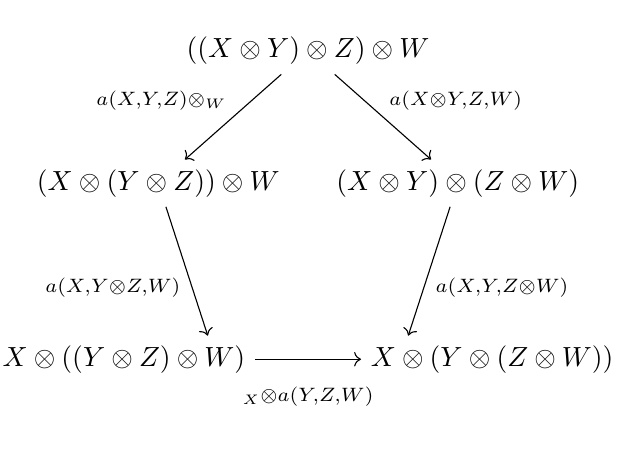
\begin{tikzpicture}[commutative diagrams/every diagram]
				\node (P0) at (90:2.3cm) {$((X \otimes Y) \otimes Z) \otimes W$};
				\node (P1) at (90+72:2cm) {$(X \otimes (Y \otimes Z)) \otimes W$} ;
				\node (P2) at (90+2*72:2cm) {\makebox[5ex][r]{$X \otimes ((Y \otimes Z) \otimes W)$}};
				\node (P3) at (90+3*72:2cm) {\makebox[5ex][l]{$X \otimes (Y \otimes (Z \otimes W))$}};
				\node (P4) at (90+4*72:2cm) {$(X \otimes Y) \otimes (Z \otimes W)$};

				\path[commutative diagrams/.cd, every arrow, every label]
				(P0) edge node[swap] {$a(X,Y,Z) \otimes \identity_W$} (P1)
				(P1) edge node[swap] {$a(X, Y \otimes Z, W)$} (P2)
				(P2) edge node[swap, inner sep=1em] {$\identity_X \otimes a(Y,Z,W)$} (P3)
				(P4) edge node {$a(X, Y, Z \otimes W)$} (P3)
				(P0) edge node {$a(X \otimes Y, Z, W)$} (P4);
			\end{tikzpicture}\end{center}
		\item objek $\munit \in \Obj(\mathcal{V})$, yang disebut objek satuan, sedemikian sehingga fungtor-fungtor $\munit \otimes -$ dan $- \otimes \munit$ memberikan ekuivalensi dari kategori $\mathcal{V}$ ke dirinya sendiri;\index{objek!objek satuan (unit object)}
		\item isomorfisme $\iota: \munit \otimes \munit \rightiso \munit$.
	\end{enumerate}
\end{definition}

Isomorfisme $a$ di atas juga disebut \emph{kendala asosiativitas}\index{jieheyueshu@kendala asosiativitas}. Kita lazim membayangkan $\otimes$ sebagai semacam operasi biner, tetapi dalam praktik $\otimes$ jarang memenuhi hukum asosiatif ketat $(X \otimes Y) \otimes Z = X \otimes (Y \otimes Z)$. Karena itu, kita mengganti kesamaan dalam hukum asosiatif dengan keluarga ``kendala'' yang ditetapkan, yaitu $a(X, Y, Z): (X \otimes Y) \otimes Z \rightiso X \otimes (Y \otimes Z)$, sedangkan $a$ natural dalam setiap peubah. Karena kendala asosiativitas dapat diterapkan berulang kali, $a$ juga harus memenuhi syarat kompatibilitas dalam (iii). Diagram komutatif tersebut disebut aksioma segilima Mac Lane\index{MacLane@aksioma segilima Mac Lane (pentagon axiom)}. Titik-titik diagramnya adalah semua cara yang mungkin untuk mengalikan $X,Y,Z,W$ secara berurutan, sedangkan dua titik dihubungkan oleh sisi jika di antara keduanya dapat diterapkan satu kendala asosiativitas $a$. Serupa dengan itu, objek satuan $\munit$ tidak memenuhi kesamaan ketat $\munit \otimes \munit = \munit$, melainkan isomorfisme natural $\iota$.

Hal ini sekali lagi memperlihatkan perbedaan antara kesamaan ketat dan isomorfisme dalam teori kategori; lihat Catatan \ref{rem:strict-or-not}.

\begin{definition}\label{def:monoidal-constraints}
	Misalkan $(\mathcal{V}, \otimes, a, \munit, \iota)$ kategori monoidal dan $X$ suatu objek. Karena $\munit \otimes -$ dan $- \otimes \munit$ memberikan ekuivalensi kategori $\mathcal{V} \to \mathcal{V}$, kita dapat
	\begin{compactitem}
		\item mendefinisikan secara tunggal $ \lambda_X: \munit \otimes X \rightiso X$ sedemikian sehingga
			\[ \identity_{\munit} \otimes \lambda_X = \left[ \munit \otimes (\munit \otimes X) \xrightarrow{ a(\munit, \munit, X)^{-1} } (\munit \otimes \munit) \otimes X \xrightarrow{\iota \otimes \identity_X} \munit \otimes X \right] ; \]
		\item mendefinisikan secara tunggal, dengan cara serupa, $\rho_X: X \otimes \munit \rightiso X$ sedemikian sehingga
			\[ \rho_X \otimes \identity_{\munit} = (\identity_X \otimes \iota) \circ a(X, \munit, \munit). \]
	\end{compactitem}
	Keduanya membentuk isomorfisme antarfungtor $\lambda: \munit \otimes \bullet \rightiso \bullet$ dan $\rho: \bullet \otimes \munit \rightiso \bullet$.
\end{definition}
Morfisme-morfisme $\lambda, \rho$ ini juga disebut kendala satuan; peran keduanya serupa dengan $a$. Kelak kita akan membuktikan $\lambda_\munit = \iota = \rho_\munit$.

Jika tidak menimbulkan kerancuan, kita sering menotasikan kategori monoidal hanya dengan $\mathcal{V}$ dan menghilangkan komponen-komponen lainnya. Jika subkategori $\mathcal{V}' \subset \mathcal{V}$ memuat objek $\munit$ dan $X,Y \in \Obj(\mathcal{V}')$ mengakibatkan $X \otimes Y \in \Obj(\mathcal{V}')$, maka $\mathcal{V}'$ disebut \emph{subkategori monoidal} dari $\mathcal{V}$. \index{yaobanfanchou@kategori monoidal (monoidal category)!subkategori monoidal (monoidal subcategory)}

\begin{example}\label{eg:monoidal-cat}
	Berikut ini semuanya merupakan kategori monoidal.
	\begin{enumerate}
		\item Jika kategori $\mathcal{C}$ mempunyai produk berhingga, ambil $\otimes := \times$ dan isomorfisme $a(X,Y,Z): (X \times Y) \times Z \rightiso X \times (Y \times Z)$ yang diberikan oleh Lema \ref{prop:product-associativity}; objek satuannya diberikan oleh objek terminal (produk kosong).
		\item Jika kategori $\mathcal{C}$ mempunyai koproduk berhingga, ambil $\otimes := \sqcup$; dengan cara serupa diperoleh kategori monoidal, dengan objek satuan diberikan oleh objek awal (koproduk kosong).
		\item Misalkan $\mathcal{C}$ kategori. Kategori endofungtor $\text{Fct}(\mathcal{C}, \mathcal{C})$ menjadi kategori monoidal terhadap komposisi fungtor $\otimes := \circ$. Perhatikan bahwa untuk morfisme $\theta: F \to G$ dan $\psi: F' \to G'$ dalam $\text{Fct}(\mathcal{C}, \mathcal{C})$, morfisme yang diinduksi ialah komposisi horizontal $\psi\theta: F'F \to G'G$; objek satuannya adalah fungtor identitas $\identity_{\mathcal{C}}$.
		\item Andaikan pembaca mempunyai pengetahuan dasar tentang teori modul. Misalkan $A$ gelanggang komutatif dan pertimbangkan kategori modul-$A$, $A\dcate{Mod}$. Terhadap hasil kali tensor $\otimes := \dotimes{A}$, kategori ini mempunyai struktur kategori monoidal yang natural; objek satuannya adalah $A$ sendiri. Lihat Korolari \ref{prop:module-monoidal-cat} untuk perinciannya.
	\end{enumerate}
\end{example}

\begin{example}[Kategori kobordisme]\label{eg:cob-cat}
	Untuk $n \in \Z_{\geq 1}$, definisikan kategori kobordisme $n\dcate{Cob}$ sebagai berikut. Semua manifold di bawah ini adalah manifold diferensial real. Objek kategori $n\dcate{Cob}$ ialah manifold kompak terorientasi tanpa batas berdimensi $n-1$, termasuk himpunan kosong $\emptyset$. Objek yang diperoleh dengan membalik orientasi $X$ dinotasikan oleh $X^*$. Himpunan morfisme antara dua objek $X, Y$ diberikan oleh kelas-kelas ekuivalensi \emph{kobordisme}, yaitu manifold terorientasi berdimensi $n$ dengan batas, $W$, yang dilengkapi isomorfisme $\partial W \rightiso X \sqcup Y^*$. Untuk $n=2$, kobordisme dapat digambarkan dengan diagram yang lazim disebut celana, digambar dari kiri ke kanan, seperti berikut:

	\begin{center}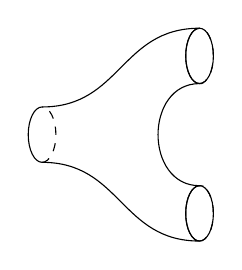
\begin{tikzpicture}[every tqft/.style={draw, boundary lower style={draw,dashed}}, tqft/flow=east]
		\node[tqft/pair of pants, draw] (a) {};
		\node[tqft boundary circle, draw] at (a.outgoing boundary 1) {};  % 3D effects
		\node[tqft boundary circle, draw] at (a.outgoing boundary 2) {};
	\end{tikzpicture} \end{center}

	Diagram ini memberikan morfisme dari lingkaran satuan $\mathbb{S}^1$ berorientasi positif ke $\mathbb{S}^1 \sqcup \mathbb{S}^1$; ``celana'' dalam diagram tersebut adalah manifold terorientasi $W$ pada definisi morfisme. Dengan demikian, komposisi morfisme tidak lain adalah menjahit kaki-kaki celana, seperti berikut:
	\begin{center}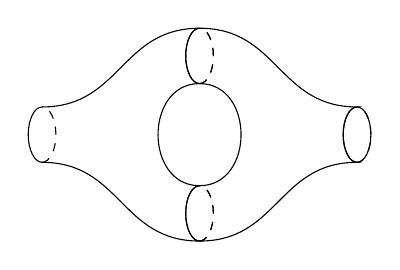
\begin{tikzpicture}[every tqft/.style={draw, boundary lower style={draw,dashed}}, tqft/flow=east]
		\node[tqft/pair of pants, draw] (a) {};
		\node[tqft/reverse pair of pants, draw, anchor=incoming boundary 1] (b) at (a.outgoing boundary 1) {};
		\node[tqft boundary circle,  draw] at (b.outgoing boundary 1) {};  % 3D effects
	\end{tikzpicture}\end{center}
	Diagram ini memberikan endomorfisme $\mathbb{S}^1$. Jelas bahwa penjahitan harus mempertahankan orientasi, yakni sisi dalam dan luar kedua kaki celana tidak boleh tertukar; selain itu, sambungan harus dibuat mulus, meskipun hal terakhir ini tidak memengaruhi gagasan utamanya.

	Morfisme identitas $\identity_X$ diberikan oleh silinder $W := X \times [0,1]$. Gabungan saling lepas $(X, Y) \mapsto X \sqcup Y$ membekali $n\dcate{Cob}$ dengan struktur kategori monoidal, dan objek satuannya adalah $\emptyset$. Karena keterbatasan ruang, kita tidak akan memeriksa perinciannya lebih lanjut. Kajian tentang kategori $n\dcate{Cob}$ dan varian-variannya merupakan salah satu pokok penting dalam topologi dan teori medan kuantum topologis.
\end{example}

Sepintas, Definisi \ref{def:monoidal-cat} dan \ref{def:monoidal-constraints} tampaknya belum mencakup semua sifat yang seharusnya dimiliki objek satuan $\munit$. Namun, sifat-sifat lainnya dapat diturunkan dari aksioma segilima dan sifat fungtorial; untuk itu kita memerlukan beberapa persiapan. Kewajaran Definisi \ref{def:monoidal-cat} akan dijelaskan secara tuntas dalam \S\ref{sec:coherence}.

\begin{lemma}[G.\ M.\ Kelly]\label{prop:Kelly}
	Untuk setiap objek $X$ dalam kategori monoidal $(\mathcal{V}, \otimes, a, \munit, \lambda, \rho)$, berlaku kesamaan-kesamaan berikut:
	\begin{align}
		\label{eqn:unit-coherence-2a} \lambda_{\munit \otimes X} = \identity \otimes \lambda_X: &  \munit \otimes (\munit \otimes X) \to \munit \otimes X, \\
		\label{eqn:unit-coherence-2b} \rho_{X \otimes \munit} = \rho_X \otimes \identity: & (X \otimes \munit) \otimes \munit \to X \otimes \munit, \\
		\label{eqn:unit-coherence-2c} \lambda_{\munit} = \rho_{\munit} = \iota: & \munit \otimes \munit \rightiso \munit.
	\end{align}
	Selain itu, untuk setiap objek $X, Y$, diagram-diagram berikut komutatif:
	\begin{equation}\label{eqn:monoidal-cat-unit}\begin{tikzcd}[column sep=tiny]
		(X \otimes \munit) \otimes Y \arrow[rr, "{a(X, \munit, Y)}"] \arrow[rd, "{\rho_X \otimes \identity}"'] & & X \otimes (\munit \otimes Y) \arrow[ld, "{\identity \otimes \lambda_Y}"] \\
		& X \otimes Y &
	\end{tikzcd} \end{equation}
	(diagram di atas juga disebut aksioma segitiga kategori monoidal)
	\begin{equation}\label{eqn:unit-coherence-1} \begin{tikzcd}[column sep=0.2ex]
		(X \otimes Y) \otimes \munit \arrow[rr] \arrow[rd, "{\rho_{X \otimes Y}}"'] & & X \otimes (Y \otimes \munit) \arrow[ld, "{\identity_X \otimes \rho_Y}"] \\
		& X \otimes Y &
	\end{tikzcd} \quad
	\begin{tikzcd}[column sep=tiny]
		(\munit \otimes X) \otimes Y \arrow[rr] \arrow[rd, "{\lambda_X \otimes \identity_Y}"'] & & \munit \otimes (X \otimes Y) \arrow[ld, "{\lambda_{X \otimes Y}}"] \\
		& X \otimes Y &
	\end{tikzcd} \end{equation}
	serta
	\begin{equation}\label{eqn:unit-coherence-3} \begin{tikzcd}[column sep=tiny]
		(\munit \otimes X) \otimes \munit \arrow[d, "{\rho_{\munit \otimes X}}"'] \arrow[rr] & & \munit \otimes (X \otimes \munit) \arrow[d, "{\lambda_{X \otimes \munit}}"] \\
		\munit \otimes X \arrow[r, "{\lambda_X}"'] & X & X \otimes \munit \arrow[l, "{\rho_X}"] \\
	\end{tikzcd}. \end{equation}
\end{lemma}
\begin{proof}
	Pertama-tama kita buktikan \eqref{eqn:unit-coherence-2a}. Naturalitas $\lambda$ menunjukkan bahwa diagram
	\[ \begin{tikzcd}
		\munit \otimes (\munit \otimes X) \arrow[r, "{\lambda_{\munit \otimes X}}"] \arrow[d, "{\identity \otimes \lambda_X}"'] & \munit \otimes X \arrow[d, "{\lambda_X}"] \\
		\munit \otimes X \arrow[r, "{\lambda_X}"'] & X
	\end{tikzcd} \]
	komutatif. Karena $\lambda_X$ merupakan isomorfisme, diperoleh $\lambda_{\munit \otimes X} = \identity \otimes \lambda_X$. Dengan mempertimbangkan simetri, diperoleh \eqref{eqn:unit-coherence-2b}.

	Sekarang perhatikan diagram
	\begin{equation}\label{eqn:coherence-aux0} \begin{tikzcd}[column sep=small, row sep=2.25em]
		((X \otimes \munit) \otimes \munit) \otimes Y \arrow[dd] \arrow[rr] \arrow[rd, "{(\rho_X \otimes \identity_\munit) \otimes \identity_Y}" description] & & (X \otimes \munit) \otimes (\munit \otimes Y) \arrow[r] \arrow[d, "{\rho_X \otimes \identity_{\munit \otimes Y}}" description] & X \otimes (\munit \otimes (\munit \otimes Y)) \arrow[ld, "{\identity_X \otimes \lambda_{\munit \otimes Y}}" description] \\
		& (X \otimes \munit) \otimes Y \arrow[r] & X \otimes (\munit \otimes Y) & \\
		(X \otimes (\munit \otimes \munit)) \otimes Y \arrow[rrr] \arrow[ru, "{(\identity_X \otimes \iota) \otimes \identity_Y}" description] & & & X \otimes ((\munit \otimes \munit) \otimes Y) \arrow[uu] \arrow[lu, "{\identity_X \otimes (\iota \otimes \identity_Y)}" description]
	  \end{tikzcd} \end{equation}
	Semua panah dalam diagram ini invertibel, sedangkan panah horizontal dan vertikal berasal dari kendala asosiativitas $a$. Aksioma segilima menyatakan bahwa batas luar persegi panjang tersebut komutatif, sedangkan komutativitas dua subdiagram trapesium (satu besar dan satu kecil) tereduksi pada naturalitas kendala asosiativitas $a$. Dari tiga subdiagram segitiga yang tersisa, jika sebarang dua di antaranya komutatif, yang ketiga pun otomatis komutatif. Sekarang kita nyatakan bahwa segitiga kanan atas komutatif. Memang, \eqref{eqn:unit-coherence-2a} memberikan $\identity \otimes \lambda_Y = \lambda_{\munit \otimes Y}: \munit \otimes (\munit \otimes Y) \rightiso \munit \otimes Y$; karena itu, definisi $\lambda_Y$ memastikan bahwa segitiga paling kanan sudah komutatif sebelum menerapkan $X \otimes -$. Dengan cara serupa, segitiga kiri juga komutatif. Karena setiap objek dalam $\mathcal{V}$ isomorfik dengan suatu $\munit \otimes Y$, hal ini membuktikan \eqref{eqn:monoidal-cat-unit}. Dengan mengambil $X=Y=\munit$ dalam \eqref{eqn:monoidal-cat-unit} dan membandingkan konstruksi $\rho_\munit, \lambda_\munit$, diperoleh $\identity \otimes \lambda_{\munit} = \identity \otimes \iota$ dan $\rho_{\munit} \otimes \identity = \iota \otimes \identity$. Dari sini diperoleh kembali \eqref{eqn:unit-coherence-2c}.

	Dengan prinsip yang sama, untuk sebarang objek $X, Y, Z$ dapat dipertimbangkan diagram
	\begin{equation*}\begin{tikzcd}[column sep=small, row sep=2.25em]
		((Z \otimes \munit) \otimes X) \otimes Y \arrow[dd] \arrow[rr] \arrow[rd, "{(\rho_Z \otimes \identity_X) \otimes \identity_Y}" description] & & (Z \otimes \munit) \otimes (X \otimes Y) \arrow[r] \arrow[d, "{\rho_Z \otimes \identity_{X \otimes Y}}" description] & Z \otimes (\munit \otimes (X \otimes Y)) \arrow[ld, "{\identity_Z \otimes \lambda_{X \otimes Y}}" description] \\
		& (Z \otimes X) \otimes Y \arrow[r] & Z \otimes (X \otimes Y) & \\
		(Z \otimes (\munit \otimes X)) \otimes Y \arrow[rrr] \arrow[ru, "{(\identity_Z \otimes \lambda_X) \otimes \identity_Y}" description] & & & Z \otimes ((\munit \otimes X) \otimes Y) \arrow[uu] \arrow[lu, "{\identity_Z \otimes (\lambda_X \otimes \identity_Y)}" description]
	\end{tikzcd}\end{equation*}
	Kita nyatakan bahwa segitiga paling kanan komutatif. Argumennya sama seperti di atas: cukup turunkan komutativitas segitiga kiri dan kanan atas dari \eqref{eqn:monoidal-cat-unit}. Dengan mengambil $Z = \munit$, diketahui bahwa diagram
	\[ \begin{tikzcd}[column sep=tiny, row sep=small]
		(\munit \otimes X) \otimes Y \arrow[rr] \arrow[rd, "{\lambda_X \otimes \identity_Y}"'] & & \munit \otimes (X \otimes Y) \arrow[ld, "{\lambda_{X \otimes Y}}"] \\
		& X \otimes Y &
	\end{tikzcd} \]
	menjadi komutatif setelah menerapkan $\munit \otimes -$, sehingga diagram semula komutatif. Dengan demikian diperoleh diagram komutatif kedua dalam \eqref{eqn:unit-coherence-1}; berdasarkan simetri, diagram pertama dalam \eqref{eqn:unit-coherence-1} juga komutatif.

	Sekarang kita buktikan bahwa diagram \eqref{eqn:unit-coherence-3} komutatif dengan menguraikannya menjadi
	\[ \begin{tikzcd}
		{} & \munit \otimes (X \otimes \munit) \arrow[rd, "{\lambda_{X \otimes \munit}}"] & \\
		(\munit \otimes X) \otimes \munit \arrow[rr, "{\lambda_X \otimes \identity}"] \arrow[d, "{\rho_{\munit \otimes X}}"'] \arrow[ru] & & X \otimes \munit \arrow[d, "{\rho_X}"] \\
		\munit \otimes X \arrow[rr, "{\lambda_X}"'] & & X
	\end{tikzcd}\]
	Naturalitas $\rho$ menunjukkan bahwa bagian persegi panjang komutatif; di sisi lain, bagian segitiga juga telah dibuktikan komutatif. Karena itu, seluruh diagram komutatif.
\end{proof}

\begin{remark}
	Sebagian pustaka (misalnya \cite{ML98}) memakai definisi kategori monoidal yang lebih rumit: isomorfisme $\lambda, \rho$ yang menyertai objek satuan $\munit$ dan aksioma segitiga \eqref{eqn:monoidal-cat-unit} semuanya menjadi bagian dari definisi.
\end{remark}

\begin{definition}\label{def:monoidal-functor}\index{yaobanhanzi@fungtor monoidal (monoidal functor)}
	Misalkan $\mathcal{V}_1$ dan $\mathcal{V}_2$ kategori monoidal. Suatu \emph{fungtor monoidal} dari $\mathcal{V}_1$ ke $\mathcal{V}_2$ adalah data $(F, \xi_F)$, dengan $F: \mathcal{V}_1 \to \mathcal{V}_2$ suatu fungtor dan
	\[ \xi_F:  F(\cdot) \otimes F(\cdot) \rightiso F(\cdot \otimes \cdot) \]
	merupakan isomorfisme antara fungtor-fungtor biner, sedemikian sehingga $\exists \varphi_F: F(\munit_1) \simeq \munit_2$ dan diagram berikut komutatif untuk semua objek $X,Y,Z$.
	\[ \begin{tikzcd}[column sep=10em]
		F((X \otimes Y) \otimes Z) \arrow[r, "{F a(X,Y,Z)}"] & F(X \otimes (Y \otimes Z)) \\
		F(X \otimes Y) \otimes F(Z) \arrow[u, "{\xi_F(X \otimes Y, Z)}"] & F(X) \otimes F(Y \otimes Z) \arrow[u, "{\xi_F(X, Y \otimes Z)}"'] \\
		(F(X) \otimes F(Y)) \otimes F(Z) \arrow[r, "{a(F(X), F(Y), F(Z))}"'] \arrow[u, "{\xi_F(X, Y) \otimes \identity}"] & F(X) \otimes (F(Y) \otimes F(Z)) \arrow[u, "{\identity \otimes \xi_F(Y, Z)}"']
	\end{tikzcd} \]
\end{definition}
Menurut konvensi, kita juga sering menghilangkan data tambahan $\xi_F$ dari notasi fungtor monoidal.

Perhatikan bahwa untuk fungtor monoidal $F$, terdapat pilihan baku bagi isomorfisme $\varphi_F: \munit_2 \rightiso F(\munit_1)$, yaitu melalui diagram-diagram berikut:
\begin{equation} \begin{tikzcd}
	\munit_2 \otimes F(\munit_1) \arrow[r, "{\lambda_2}"] \arrow[d, "{\varphi_F \otimes \identity}"'] & F(\munit_1) \arrow[d, "{F(\iota_1)^{-1}}"] \\
	F(\munit_1) \otimes F(\munit_1) \arrow[r, "{\xi_F}"'] & F(\munit_1 \otimes \munit_1)
\end{tikzcd} \quad
\begin{tikzcd}
	F(\munit_1) \otimes \munit_2  \arrow[r, "{\rho_2}"] \arrow[d, "{\identity \otimes \varphi_F}"'] & F(\munit_1) \arrow[d, "{F(\iota_1)^{-1}}"] \\
	F(\munit_1) \otimes F(\munit_1) \arrow[r, "{\xi_F}"'] & F(\munit_1 \otimes \munit_1)
\end{tikzcd} \end{equation}
Komutativitas kedua diagram tersebut ekuivalen dan menentukan $\varphi_F$ yang sama (lihat \cite[Proposition 2.4.3]{EGNO15}). Lebih umum lagi, untuk setiap $X$ terdapat diagram komutatif
\begin{equation}\label{eqn:monoidal-functor-units} \begin{tikzcd}
	\munit_2 \otimes F(X) \arrow[r, "{\lambda_2}"] \arrow[d, "{\varphi_F \otimes \identity}"'] & F(X) \arrow[d, "{F(\lambda_X)^{-1}}"] \\
	F(\munit_1) \otimes F(X) \arrow[r, "{\xi_F}"'] & F(\munit_1 \otimes X)
\end{tikzcd} \quad
\begin{tikzcd}
	F(X) \otimes \munit_2 \arrow[r, "{\rho_2}"] \arrow[d, "{\identity \otimes \varphi_F}"'] & F(X) \arrow[d, "{F(\rho_X)^{-1}}"] \\
	F(X) \otimes F(\munit_1) \arrow[r, "{\xi_F}"'] & F(X \otimes \munit_1)
\end{tikzcd} \end{equation}
Karena kegunaannya terbatas, kita tidak membuktikan ekuivalensi ini secara terperinci. Petunjuk: mulai dari diagram pertama untuk mendefinisikan $\varphi_F$, lalu terapkan $F(X) \otimes \bullet$ pada seluruh diagram dan gunakan sifat kendala asosiativitas, objek satuan, dan $\xi_F$; akhirnya batalkan $F(\munit_1)$ di sebelah kanan secara tepat untuk memperoleh diagram komutatif keempat. Argumen lainnya diserahkan kepada pembaca.

\begin{remark}
	Dalam banyak pustaka, fungtor monoidal yang didefinisikan di atas disebut \emph{fungtor monoidal kuat}; komutativitas \eqref{eqn:monoidal-functor-units} dan isomorfisme $\varphi_F: \munit_2 \rightiso F(\munit_1)$ menjadi bagian dari definisi. Dalam kerangka ini, jika $\xi_F: F(\cdot) \otimes F(\cdot) \to F(\cdot \otimes \cdot)$ dan $\varphi_F: \munit_2 \to F(\munit_1)$ tidak disyaratkan merupakan isomorfisme, data $(F, \xi_F, \varphi_F)$ disebut \emph{fungtor monoidal longgar-kanan}; dengan membalik panah-panah dalam data tersebut menjadi $\eta_F: F(\cdot \otimes \cdot) \to F(\cdot) \otimes F(\cdot)$ dan $\psi_F: F(\munit_1) \to \munit_2$, serta menyesuaikan \eqref{eqn:monoidal-functor-units}, diperoleh \emph{fungtor monoidal longgar-kiri}. Pembaca tidak perlu menghafalkannya; bila diperlukan, kita akan membedakannya secara eksplisit. \index{yaobanhanzi@fungtor monoidal!longgar-kiri/longgar-kanan (left-lax/right-lax)}
\end{remark}

\begin{example}
	Andaikan kategori $\mathcal{C}_1$, $\mathcal{C}_2$ mempunyai produk berhingga, sehingga dapat dipandang sebagai kategori monoidal ($\otimes := \times$, $\munit := \text{objek terminal}$). Setiap fungtor $F: \mathcal{C}_1 \to \mathcal{C}_2$ dilengkapi morfisme natural $\eta_F: F(\cdot \otimes \cdot) \to F(\cdot) \otimes F(\cdot)$, yang memberikan struktur fungtor monoidal longgar-kiri secara natural pada $F$ (lihat Definisi \ref{def:preservation-limit}); $F$ merupakan fungtor monoidal jika dan hanya jika $F$ mempertahankan produk berhingga.
\end{example}

\begin{definition}\index{ziranbianhuan@transformasi natural!kasus monoidal}
	Misalkan $F, G: \mathcal{V}_1 \to \mathcal{V}_2$ fungtor monoidal. Suatu transformasi natural (atau morfisme) di antaranya, yang dinotasikan dengan $\theta$, adalah transformasi natural sedemikian sehingga $\theta_{\munit_1}$ merupakan isomorfisme dan diagram berikut komutatif untuk semua $X, Y$:
	\[ \begin{tikzcd}[column sep=huge]
		F(X) \otimes F(Y) \arrow[r, "{\xi_F(X, Y)}"] \arrow[d, "{\theta_X \otimes \theta_Y}"'] & F(X \otimes Y) \arrow[d, "{\theta_{X \otimes Y}}"] \\
		G(X) \otimes G(Y) \arrow[r, "{\xi_G(X, Y)}"'] & G(X \otimes Y) .
	\end{tikzcd} \]
	Sebagai latihan, buktikan bahwa bagi $\varphi_F$ dan $\varphi_G$ baku selalu berlaku $\varphi_G = \theta_{\mathbf{1}_1} \varphi_F$.
\end{definition}

Fungtor monoidal dan transformasi natural mempunyai operasi komposisi yang jelas. Dengan operasi ini dapat didefinisikan isomorfisme dan ekuivalensi kategori monoidal; lihat Definisi \ref{def:cat-equivalence}. Untuk membedakannya, ekuivalensi antara kategori monoidal kadang-kadang disebut pula ekuivalensi monoidal.\index{fanchoudengjia@ekuivalensi kategori!kasus monoidal}
\section{Keketatan dan Teorema Koherensi}\label{sec:coherence}
Karena hukum asosiatif dan unsur satuan dalam kategori monoidal hanya ditentukan hingga isomorfisme, diperlukan usaha cukup besar untuk membuktikan berbagai sifat intuitifnya, yang dinyatakan melalui beragam diagram komutatif. Namun, setidaknya masih ada dua pertanyaan:
\begin{compactenum}[(i)]
	\item Dapatkah kita dalam praktik mereduksi pembahasan pada kasus dengan hukum asosiatif dan unsur satuan yang berlaku secara ketat?
	\item Apakah Definisi \ref{def:monoidal-cat} sudah mencakup seluruh sifat yang kita harapkan dari kategori monoidal? Lebih konkretnya, dari fungtor biner $\otimes$, kendala asosiativitas $a$, serta kendala satuan $\lambda, \rho$, dapat dibentuk sangat banyak diagram yang semuanya bersifat ``natural'' dan semestinya komutatif. Dapatkah seluruh sifat tersebut diturunkan dari aksioma segilima Mac Lane dan sifat $\iota: \munit \otimes \munit \rightiso \munit$?
\end{compactenum}
Kedua pertanyaan ini berkaitan erat. Untuk pertanyaan (i), mula-mula kita perkenalkan konsep \emph{kategori monoidal ketat}.

\begin{definition}\label{def:strict-monoidal-cat}\index{yaobanfanchou@kategori monoidal (monoidal category)!kategori monoidal ketat (strict monoidal category)}
	Kategori monoidal $\mathcal{V}$ disebut ketat jika
	\begin{compactitem}
		\item kendala asosiativitas $a$ berupa kesamaan, yakni $(X \otimes Y) \otimes Z = X \otimes (Y \otimes Z)$;
		\item kendala satuan $\lambda, \rho$ berupa kesamaan, yakni $X \otimes \munit = \munit \otimes X = X$.
	\end{compactitem}
	Di sini $X,Y,Z$ menyatakan sebarang objek dalam $\mathcal{V}$.
\end{definition}
Dalam kategori monoidal ketat, hasil kali $\otimes$ sebarang banyak objek dapat ditulis sebagai $X_1 \otimes X_2 \otimes X_3 \cdots$ tanpa menimbulkan ambiguitas. Dalam keadaan ini, pertanyaan (ii) juga mendapat jawaban afirmatif karena setiap diagram yang dibangun dari kendala asosiativitas dan kendala satuan hanya mempunyai satu jenis panah, yaitu kesamaan.

Teori kategori monoidal ketat jelas jauh lebih sederhana. Semua argumen dalam \S\ref{sec:monoidal-cat-def} menjadi tautologi dalam kasus ketat. Kategori $\text{Fct}(\mathcal{C}, \mathcal{C})$ pada Contoh \ref{eg:monoidal-cat} merupakan contoh khas kategori monoidal ketat. Di luar itu, kategori monoidal yang lazim dalam aljabar umumnya tidak ketat. Hal ini kembali memperlihatkan kerumitan pertanyaan (ii). Hasil Mac Lane berikut \cite[VII.2]{ML98} memberikan jawaban afirmatif.

\begin{theorem}[S.\ Mac Lane]\label{prop:ML-coherence}\index{MacLane@Teorema koherensi Mac Lane (Mac Lane's Coherence Theorem)}
	Setiap kategori monoidal $\mathcal{V}$ ekuivalen secara monoidal dengan suatu kategori monoidal ketat.
\end{theorem}

Teorema \ref{prop:ML-coherence} juga disebut teorema koherensi. Dalam arti yang lebih luas, koherensi berarti bahwa suatu kelas diagram dalam kategori bersifat komutatif. Hasil semacam ini relatif jarang dalam teori kategori. Argumen berikut diambil dari \cite[pp.26--27]{JS93} dan \cite[\S 2.8]{EGNO15}; di sini kita hanya memberikan garis besarnya. Misalkan $\mathcal{V}$ kategori monoidal. Definisikan kategori monoidal baru $\mathbf{e}(\mathcal{V})$ sebagai berikut:
\begin{compactitem}
	\item Objek: berbentuk $(F, \rho)$, dengan $F: \mathcal{V} \to \mathcal{V}$ suatu fungtor dan
		\[ \rho = \left( \rho(X, Y): FX \otimes Y \rightiso F(X \otimes Y) \right)_{X, Y \in \Obj(\mathcal{V})} \]
		merupakan morfisme antarfungtor sedemikian sehingga diagram berikut selalu komutatif.
		\begin{center}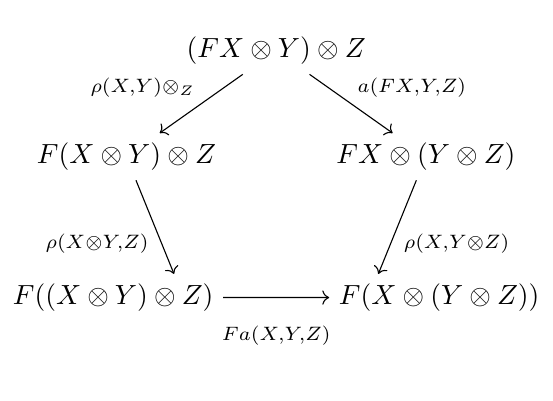
\begin{tikzpicture}[commutative diagrams/every diagram, yscale=0.8]
			\node (P0) at (90:2.3cm) {$(FX \otimes Y) \otimes Z$};
			\node (P1) at (90+72:2cm) {$F(X \otimes Y) \otimes Z$} ;
			\node (P2) at (90+2*72:2cm) {\makebox[5ex][r]{$F((X \otimes Y) \otimes Z)$}};
			\node (P3) at (90+3*72:2cm) {\makebox[5ex][l]{$F(X \otimes (Y \otimes Z))$}};
			\node (P4) at (90+4*72:2cm) {$FX \otimes (Y \otimes Z)$};

			\path[commutative diagrams/.cd, every arrow, every label]
			(P0) edge node[swap] {$\rho(X,Y) \otimes \identity_Z$} (P1)
			(P1) edge node[swap] {$\rho(X \otimes Y, Z)$} (P2)
			(P2) edge node[swap, inner sep=1em] {$Fa(X, Y, Z)$} (P3)
			(P4) edge node {$\rho(X, Y \otimes Z)$} (P3)
			(P0) edge node {$a(FX, Y, Z)$} (P4);
		\end{tikzpicture}\end{center}
	\item Morfisme: morfisme dari $(F_1, \rho_1)$ ke $(F_2, \rho_2)$ adalah transformasi natural $\theta: F_1 \to F_2$ yang kompatibel dengan $\rho$, yakni diagram
		\[ \begin{tikzcd}
			F_1(X) \otimes Y \arrow[r, "{\rho_1}"] \arrow[d, "{\theta_X \otimes \identity_Y}"'] & F_1(X \otimes Y) \arrow[d, "{\theta_{X \otimes Y}}"] \\
			F_2(X) \otimes Y \arrow[r, "{\rho_2}"'] & F_2(X \otimes Y)
		\end{tikzcd} \]
		komutatif untuk semua $X, Y$; komposisi morfisme didefinisikan sebagai komposisi vertikal transformasi natural.
	\item Objek satuan: ambil $\munit$ sebagai fungtor identitas $\identity: \mathcal{V} \to \mathcal{V}$, dengan $\rho(X, Y) := \identity_{X \otimes Y}$.
	\item Definisikan $(F_1, \rho_1) \otimes (F_2, \rho_2)$ sebagai fungtor $F_1 F_2: \mathcal{V} \to \mathcal{V}$ bersama keluarga isomorfisme $\rho_3(X,Y)$ yang diberikan oleh komposisi
		\[ (F_1 F_2 X) \otimes Y \xrightarrow{\rho_1(F_2 X, Y)} F_1 (F_2 X \otimes Y) \xrightarrow{F_1 \rho_2(X, Y)} F_1 F_2 (X \otimes Y) \]
		dengan $X, Y \in \Obj(\mathcal{V})$.
\end{compactitem}

\begin{lemma}
	$\mathbf{e}(\mathcal{V})$ merupakan kategori monoidal ketat.
\end{lemma}
\begin{proof}
	Verifikasi langsung.
\end{proof}

Secara kasar, definisi $\mathbf{e}(\mathcal{V})$ menyatakan bahwa $F$ harus ``berkomutasi'' dengan perkalian kanan yang ditentukan oleh $\otimes$, sedangkan data $\rho$ berfungsi sebagai ``saksi'' bagi komutasi tersebut. Sifat objek satuan kemudian memperlihatkan bahwa $F$ sepenuhnya ditentukan oleh $F(\munit)$ dan $\rho$. Pernyataan tepatnya adalah hasil berikut.
\begin{lemma}
	Definisikan fungtor $L: \mathcal{V} \to \mathbf{e}(\mathcal{V})$ sehingga untuk setiap objek $X$ berlaku
	\[ LX = X \otimes -: \mathcal{V} \to \mathcal{V} \]
	dengan $\rho(Y, Z)$ yang bersesuaian diberikan oleh kendala asosiativitas $a(X, Y, Z)$. Pada tingkat morfisme, definisikan $Lf = f \otimes -$. Maka $L$ merupakan fungtor penuh, setia, dan surjektif secara esensial, serta mempunyai struktur fungtor monoidal yang natural.
\end{lemma}
\begin{proof}[Garis besar]
	Fungtor $L$ terdefinisi dengan baik berkat aksioma segilima pada $\mathcal{V}$. Struktur fungtor monoidalnya ditentukan oleh isomorfisme yang jelas $L\munit \rightiso \munit$ dan keluarga isomorfisme $\xi_L(X_1, X_2): LX_1 \otimes LX_2 \rightiso L(X_1 \otimes X_2)$ yang diberikan oleh kendala asosiativitas. Selanjutnya, periksa bahwa
	\begin{compactitem}
		\item $L$ surjektif secara esensial: sesungguhnya $(F, \rho) \simeq L(F(\munit))$,
		\item $L$ penuh dan setia: pemetaan invers $\Hom_{\mathbf{e}(\mathcal{V})}(LX, LY) \to \Hom_{\mathcal{V}}(X, Y)$ memetakan $\theta: LX \to LY$ ke
			\[ X \rightiso X \otimes \munit = LX(\munit) \xrightarrow{\theta_\munit} LY(\munit) = Y \otimes \munit \rightiso Y. \]
	\end{compactitem}
	Pembaca yang berminat dipersilakan melengkapi perinciannya atau membaca rujukan yang diberikan.
\end{proof}
Kedua lema sebelumnya bersama-sama membuktikan Teorema \ref{prop:ML-coherence}.

\section{Struktur Kepang}\label{sec:braiding}
Operasi $\otimes$ dalam kategori monoidal umumnya tidak disyaratkan komutatif. Namun, dalam banyak contoh, fenomena komutativitas tidak hanya hadir tetapi juga sangat penting. Tujuan struktur kepang ialah menjelaskan komutativitas operasi $\otimes $. Seperti pada objek satuan dan hukum asosiatif, yang diperlukan di sini adalah suatu keluarga isomorfisme, bukan kesamaan ketat; keluarga ini juga disebut \emph{kendala komutativitas}. Asal penamaan struktur kepang akan dijelaskan dalam Contoh \ref{eg:braid}. Salah satu sumber awalnya adalah \cite{JS93}.

\begin{definition}\label{def:braiding}\index{bianjiegou@struktur kepang (braiding)}\index{liujiaoxinggongli@aksioma segienam (hexagon axiom)}
	Misalkan $(\mathcal{V}, \otimes, a, \munit, \iota)$ kategori monoidal. Suatu \emph{struktur kepang} pada kategori ini berarti isomorfisme antara fungtor biner
	\[ c(X,Y): X \otimes Y \rightiso Y \otimes X, \quad X, Y \in \Obj(\mathcal{V}) \]
	(yakni, natural terhadap peubah $X, Y$), sedemikian sehingga diagram-diagram berikut komutatif:
	\begin{equation}\label{eqn:hexagon-axiom-1}\begin{tikzcd}[row sep=small]
		{} & X \otimes (Y \otimes Z) \arrow[r, "{c(X, Y \otimes Z)}" inner sep=1em] & (Y \otimes Z) \otimes X \arrow[rd] & \\
		(X \otimes Y) \otimes Z \arrow[ru] \arrow[rd, "{c(X,Y) \otimes \identity}"'] & & & Y \otimes (Z \otimes X) \\
		& (Y \otimes X) \otimes Z \arrow[r] & Y \otimes (X \otimes Z) \arrow[ru, "{\identity \otimes c(X,Z)}"'] &
	\end{tikzcd}\end{equation}
	\begin{equation}\label{eqn:hexagon-axiom-2}\begin{tikzcd}[row sep=small]
		{} & (X \otimes Y) \otimes Z \arrow[r, "{c(X \otimes Y, Z)}" inner sep=1em] & Z \otimes (X \otimes Y) \arrow[rd] & \\
		X \otimes (Y \otimes Z) \arrow[ru] \arrow[rd, "{\identity \otimes c(Y, Z)}"'] & & & (Z \otimes X) \otimes Y \\
		& X \otimes (Z \otimes Y) \arrow[r] & (X \otimes Z) \otimes Y \arrow[ru, "{c(X, Z) \otimes \identity}"'] &
	\end{tikzcd}\end{equation}
	serta
	\begin{equation}\begin{tikzcd}
		\munit \otimes X \arrow[rd, "\lambda_X"'] \arrow[rr, "{c(\munit, X)}"] & & X \otimes \munit \arrow[ld, "\rho_X"] \\
		& X &
	\end{tikzcd} \quad \begin{tikzcd}
		X \otimes \munit \arrow[rd, "\rho_X"'] \arrow[rr, "{c(X, \munit)}"] & & \munit  \otimes X \arrow[ld, "\lambda_X"] \\
		& X &
	\end{tikzcd}\end{equation}
	dengan $X,Y,Z$ sebarang objek dalam $\mathcal{V}$; semua panah tanpa label adalah kendala asosiativitas atau inversnya.
\end{definition}

Kategori monoidal yang dilengkapi struktur kepang $c$ singkatnya disebut kategori monoidal berkepang. Diagram \eqref{eqn:hexagon-axiom-1} dan \eqref{eqn:hexagon-axiom-2} umumnya disebut aksioma segienam.
\begin{remark}\label{rem:hexagon-axiom-strict}
	Untuk kategori monoidal ketat (Definisi \ref{def:strict-monoidal-cat}), aksioma segienam dapat ditulis sebagai
	\begin{align*}
		c(X \otimes Y, Z) & = (c(X, Z) \otimes \identity_Y) (\identity_X \otimes c(Y, Z)), \\
		c(X, Y \otimes Z) & = (\identity_Y \otimes c(X, Z)) (c(X, Y) \otimes \identity_Z)
	\end{align*}
\end{remark}

\begin{definition}\index{yaobanhanzi@fungtor monoidal (monoidal functor)!berkepang (braided)}
	Misalkan $\mathcal{V}_1, \mathcal{V}_2$ kategori monoidal. Fungtor monoidal $F: \mathcal{V}_1 \to \mathcal{V}_2$ disebut fungtor monoidal berkepang jika memenuhi sifat berikut: untuk sebarang objek $X, Y$, diagram berikut komutatif.
	\[ \begin{tikzcd}[column sep=small]
		FX \otimes FY \arrow[r] \arrow[d, "{c_2(FX, FY)}"'] & F(X \otimes Y) \arrow[d, "{Fc_1(X, Y)}"] \\
		FY \otimes FX \arrow[r] & F(Y \otimes X)
	\end{tikzcd} \]
\end{definition}

\begin{definition}\label{def:symm-monoidal-cat}\index{yaobanfanchou@kategori monoidal (monoidal category)!kategori monoidal simetris (symmetric monoidal category)}
	Misalkan $(\mathcal{V}, \otimes, a, \munit, \iota, c)$ kategori monoidal berkepang. Jika syarat simetri $c(Y,X) \circ c(X, Y) = \identity_{X \otimes Y}$ berlaku untuk semua $X, Y$, kategori tersebut disebut \emph{kategori monoidal simetris}.
\end{definition}

\begin{example}
	Kategori-kategori monoidal yang dibangun dari produk dan koproduk dalam Contoh \ref{eg:monoidal-cat} semuanya mempunyai struktur kepang yang natural (lihat Lema \ref{prop:product-commutativity}). Demikian pula, kategori modul atas gelanggang komutatif $R$, yakni $R\dcate{Mod}$, mempunyai struktur kepang natural sebagai berikut:
	\begin{align*}
		c(M, N): M \dotimes{R} N & \longrightarrow N \dotimes{R} M \\
		m \otimes n & \longmapsto n \otimes m, \quad m \in M, n \in N.
	\end{align*}
	Semua kategori monoidal berkepang ini bersifat simetris. Perinciannya dapat dilihat dalam \S\ref{sec:module-tensor-prod}.
\end{example}

\begin{proposition}[Persamaan Yang--Baxter]\label{prop:YBE-cat-strict}\index{YBE@persamaan Yang--Baxter (Yang--Baxter equation)}
	Misalkan $\mathcal{V}$ kategori monoidal berkepang. Bagian yang digambar dengan garis utuh pada diagram berikut komutatif untuk sebarang objek $X, Y, Z$.
	\begin{center}\small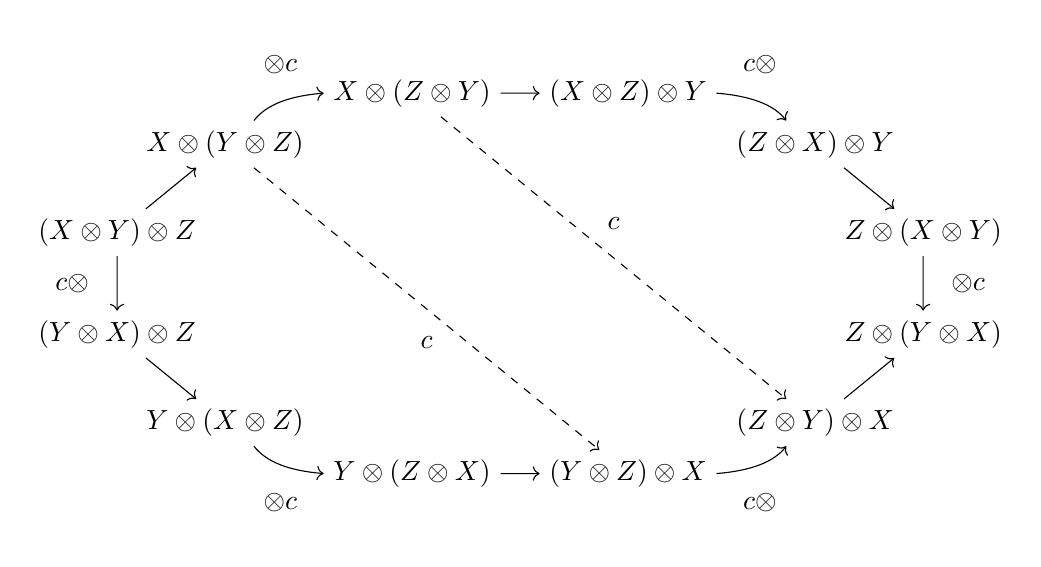
\begin{tikzpicture}[xscale=5.3, yscale=2.5, every edge/.style={draw, ->}, C/.style={inner sep=1em}]
		\node (A1) at (75:1cm) {$(X \otimes Z) \otimes Y$};
		\node (A2) at (105:1cm) {$X \otimes (Z \otimes Y)$};
		\node (A3) at (135:1cm) {$X \otimes (Y \otimes Z)$};
		\node (A4) at (165:1cm) {$(X \otimes Y) \otimes Z$};
		\node (A5) at (195:1cm) {$(Y \otimes X) \otimes Z$};
		\node (A6) at (225:1cm) {$Y \otimes (X \otimes Z)$};
		\node (A7) at (255:1cm) {$Y \otimes (Z \otimes X)$};
		\node (A8) at (285:1cm) {$(Y \otimes Z) \otimes X$};
		\node (A9) at (315:1cm) {$(Z \otimes Y) \otimes X$};
		\node (A10) at (345:1cm) {$Z \otimes (Y \otimes X)$};
		\node (A11) at (15:1cm) {$Z \otimes (X \otimes Y)$};
		\node (A12) at (45:1cm) {$(Z \otimes X) \otimes Y$};

		\draw (A4) edge (A3);	\draw (A3) edge[bend left] node[C, above] {$\identity \otimes c$} (A2); \draw (A2) edge (A1); \draw (A1) edge[bend left] node[C, above] {$c \otimes \identity$} (A12); \draw (A12) edge (A11); \draw (A11) edge node[C, right] {$\identity \otimes c$} (A10);

		\draw (A4) edge node[C, left] {$c \otimes \identity$} (A5); \draw (A5) edge (A6); \draw (A6) edge[bend right] node[C, below] {$\identity \otimes c$} (A7); \draw (A7) edge (A8); \draw (A8) edge[bend right] node[C, below] {$c \otimes \identity$} (A9); \draw (A9) edge (A10);
	
		\draw[dashed] (A3) edge node[C, below] {$c$} (A8);
		\draw[dashed] (A2) edge node[C, above] {$c$} (A9);
	\end{tikzpicture}\end{center}
	Di sini semua panah tanpa label adalah kendala asosiativitas, sedangkan $c$ menyatakan kendala komutativitas yang jelas dari konteks.
\end{proposition}
\begin{proof}
	Garis-garis putus-putus membagi diagram besar menjadi tiga bagian. Bagian kiri dan kanan komutatif karena aksioma segienam. Segi empat di tengah komutatif karena naturalitas $c$. Jadi, seluruh diagram komutatif.
\end{proof}

\begin{remark}\label{rem:YBE-cat-strict}
	Jika $\mathcal{V}$ kategori monoidal ketat, diagram di atas menyusut menjadi enam suku dan komutativitasnya tidak lain menyatakan
	\begin{multline*}
		(c(Y,Z) \otimes \identity_X) \, (\identity_Y \otimes c(X, Z)) \, (c(X, Y) \otimes \identity_Z) = \\
		(\identity_Z \otimes c(X, Y)) \, (c(X, Z) \otimes \identity_Y) \, (\identity_X \otimes c(Y, Z)).
	\end{multline*}
	Jika $\mathcal{V}$ adalah kategori ruang vektor yang membentuk kategori monoidal berkepang terhadap hasil kali tensor dan $X=Y=Z$, kesamaan di atas berkaitan dengan persamaan Yang--Baxter dalam fisika statistik (``Yang'' merujuk kepada Chen-Ning Yang). Penjelasan lebih lanjut akan diberikan dalam latihan.
\end{remark}

\begin{example}\label{eg:braid}\index[sym1]{Braid@$\cate{Braid}$}
	Berikut ini kita membangun kategori kepang \cate{Braid} dari sudut pandang topologis. Misalkan $n \in \Z_{\geq 1}$ dan definisikan
	\[ C_n := \left\{ \text{subhimpunan}\; c \subset \R^2: |c|=n \right\}, \]
	atau, dengan kata lain, ruang hasil bagi $\left\{ (y_1, \ldots, y_n) \in (\R^2)^n: \text{unsur-unsurnya berbeda} \right\}$ oleh aksi grup permutasi; ruang ini secara natural dilengkapi suatu topologi. Mulai sekarang, tetapkan $p = \{p_1, \ldots, p_n\} \in C_n$. Sebuah kepang dengan $n$ untai didefinisikan sebagai peta kontinu $x: [0,1] \to C_n$ yang memenuhi $x(0) = x(1) = p$. Secara visual, jika waktu $t$ dijadikan sumbu vertikal, lintasan $x$ memberikan $n$ kurva kontinu dalam $\R^3$ yang masing-masing tidak berpotongan dengan dirinya sendiri dan saling tidak berpotongan, serta bergerak naik dari $\{(p_1, 0), \ldots, (p_n, 0) \}$ ke $\{ (p_1, 1), \ldots, (p_n, 1) \}$; inilah yang disebut kepang. Jika kepang $x_1$ dapat dideformasi secara kontinu menjadi $x_2$ dengan titik-titik ujung $p$ tetap sepanjang deformasi, maka $x_1$ dan $x_2$ disebut ekuivalen. Selanjutnya, istilah kepang selalu berarti kelas ekuivalensi. Himpunan semua kepang dengan $n$ untai dinotasikan dengan $\mathcal{B}_n$.

	Meskipun kepang dapat dipandang sebagai gambar dalam $\R^3$, kita lazim meratakannya pada suatu bidang $L \simeq \R^2$. Proses ini dapat membuat proyeksi kurva-kurva tersebut berpotongan, tetapi dengan perturbasi kecil pada $L$ dapat dipastikan bahwa proyeksi tiga kurva tidak pernah bertemu pada satu titik. Tanpa mengurangi keumuman, dapat pula diasumsikan bahwa ujung-ujung bawah dan atas kepang masing-masing dipetakan ke $(i, 0), (i, 1) \in \R^2$, dengan $i=1, \ldots, n$. Untuk mempertahankan informasi ruangnya, pada setiap titik potong proyeksi dua kurva kita tandai kurva mana yang melintas di atas dan mana yang di bawah. Sebagai contoh, perhatikan kasus $n=3$:
	\begin{center}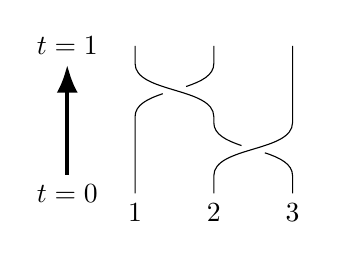
\begin{tikzpicture}[baseline=(braid), yscale=0.75]
		\braid[style strands={1}, style strands={2}, style strands={3}] (braid) s_1 s_2^{-1};
		\node[left=1em] (A) at (braid-1-s) {$t=1$};
		\node[left=1em] (B) at (braid-2-e) {$t=0$};
		\draw[-Latex, ultra thick] (B) -- (A);
		\node[below] at (braid-1-e) {$3$};
		\node[below] at (braid-2-e) {$1$};
		\node[below] at (braid-3-e) {$2$};
	\end{tikzpicture} \quad dan \quad 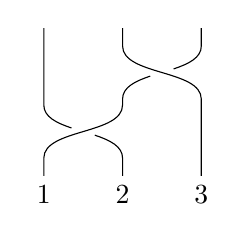
\begin{tikzpicture}[baseline=(braid), yscale=0.75]
		\braid[style strands={1}, style strands={2}, style strands={3}] (braid)  s_2 s_1^{-1};
		\node[below] at (braid-1-e) {$2$};
		\node[below] at (braid-2-e) {$3$};
		\node[below] at (braid-3-e) {$1$};
	\end{tikzpicture}\end{center}

	Untuk sebarang $x, y \in \mathcal{B}_n$, definisikan komposisi $xy$ dengan menyambungkan peta $x,y: [0,1] \to C_n$ dari ujung ke ujung; secara visual, ini berarti merekatkan ujung awal $x$ pada ujung akhir $y$ untuk memperoleh kepang baru. Mudah dilihat bahwa operasi ini terdefinisi dengan baik. Sebagai contoh, jika kedua kepang di atas berturut-turut dinotasikan dengan $x,y$, maka
	\[ xy \; = \;
		\begin{array}{|c|c|} \hline x \\ \hline y \\ \hline \end{array} \quad = \quad
		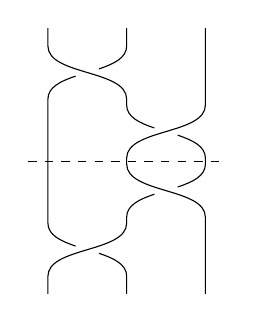
\begin{tikzpicture}[yscale=0.75, baseline=(braid)]
		\braid[style strands={1}, style strands={2}, style strands={3},
			floor command={
			\draw[dashed] (\floorsx,\floorsy) -- (\floorex,\floorsy);
			}] (braid)
		s_1 s_2^{-1} | s_2 s_1^{-1};
	\end{tikzpicture}\]
	Dengan meluruskan setiap untai pada gambar di atas, terlihat bahwa kepang tersebut ekuivalen dengan tiga untai vertikal $\vert\;\vert\;\vert$. Dari sudut pandang aljabar, $\mathcal{B}_n$ bersama operasi komposisi kepang membentuk grup yang disebut \emph{grup kepang Artin}. Asosiativitas perkalian sudah jelas, sedangkan unsur satuannya adalah $\underbracket{\vert \cdots \vert}_{n \text{untai}}$, atau, dengan kata lain, fungsi konstan $[0,1] \to \{p\} \subset C_n$. Invers suatu kepang $x$ diperoleh dengan menelusuri kurva $x: [0,1] \to C_n$ dalam arah sebaliknya, atau, setelah diratakan pada bidang $\R^2$, dengan mengambil cerminan vertikalnya. Pembaca yang mengenal topologi akan segera melihat bahwa $\mathcal{B}_n = \pi_1(C_n, p)$; lihat Contoh \ref{eg:fundamental-groupoid}.

	Dengan konvensi, $\mathcal{B}_0$ adalah grup trivial. Dalam \S\ref{sec:symmetric-group}, kita akan menyelidiki beberapa sifat $\mathcal{B}_n$ dari sudut pandang teori grup serta hubungannya dengan grup simetris $\mathfrak{S}_n$; suatu presentasi grup $\mathcal{B}_n$ akan diberikan dalam \eqref{eqn:braid-presentation}.\index{bianqun@grup kepang (braid group)}\index[sym1]{B_n@$\mathcal{B}_n$}

	Sekarang kita bangun kategori monoidal ketat $\cate{Braid}$: himpunan objeknya adalah $\Z_{\geq 0}$, sedangkan himpunan morfisme antara sebarang dua objek $n,m$ didefinisikan sebagai $\mathcal{B}_n$ jika $n=m$, dan sebagai himpunan kosong jika tidak. Komposisi morfisme adalah komposisi dalam grup kepang. Selanjutnya, definisikan $m \otimes n := m+n$; untuk $x \in \mathcal{B}_m$, $y \in \mathcal{B}_n$, morfisme $x \otimes y \in \mathcal{B}_{m+n}$ didefinisikan dengan menempatkan kedua kepang berdampingan, yang secara visual dinyatakan sebagai
	\begin{center} 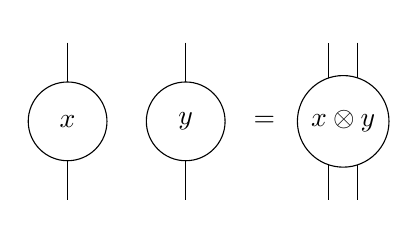
\begin{tikzpicture}[baseline=(current bounding box.center),
		 midbraid/.style={midway, draw, fill=white, shape=circle, minimum size=1cm} ]
		\draw (0,1) -- (0,-1) node[midbraid] {$x$};
		\draw (1.5,1) -- (1.5,-1) node[midbraid] {$y$};
		\node at (2.5,0) {$=$};
		\draw[double distance=10pt] (3.5, 1) -- (3.5,-1) node[midbraid] {$x \otimes y$};
	\end{tikzpicture}\end{center}
	Jelas bahwa $x \otimes y$ terdefinisi dengan baik, dan operasi ini menjadikan $\cate{Braid}$ kategori monoidal ketat; objek satuannya adalah $0$.

	Sekarang definisikan kendala komutativitas $c$ untuk memperoleh kategori monoidal berkepang. Untuk $X=m$, $Y=n$, kita menggunakan
	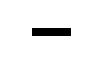
\begin{tikzpicture} \draw[black, line width=3pt] (0,0) -- (0.5, 0); \end{tikzpicture}
	untuk menyatakan $m$ untai tak terjalin yang bersesuaian dengan objek $X$, sedangkan
	
\begin{tikzpicture} \draw[lightgray, line width=3pt] (0,0) -- (0.5, 0); \end{tikzpicture}
	menyatakan $n$ untai tak terjalin yang bersesuaian dengan objek $Y$. Definisikan $c(X, Y) \in \mathcal{B}_{m+n}$ sebagai
	\[ c(m,n) \;= \; 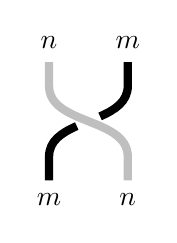
\begin{tikzpicture}[baseline=(braid)]
		\braid[style strands={1}{lightgray}, style strands={2}{black}, line width=3pt] (braid) s_1;
		\node[above] at (braid-1-s) {$n$};
		\node[above] at (braid-2-s) {$m$};
		\node[below] at (braid-1-e) {$n$};
		\node[below] at (braid-2-e) {$m$};
	\end{tikzpicture}\]
	Ini berarti bahwa $n$ untai 
\begin{tikzpicture} \draw[lightgray, line width=3pt] (0,0)--(0.5,0); \end{tikzpicture} dipandang sebagai satu kesatuan dan dilintaskan di atas $m$ untai yang dinyatakan oleh 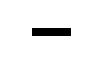
\begin{tikzpicture} \draw[black, line width=3pt] (0,0)--(0.5,0); \end{tikzpicture}. Jika $X$ atau $Y$ selanjutnya dibagi menjadi dua kelompok $U, V$ dan diagram kepang yang bersesuaian digambar (berbentuk
	
\begin{tikzpicture}[baseline=(current bounding box.center), scale=0.4, wline/.style={color=white, line width=1.8mm}]
		\draw (1,2) -- (0,0);
		\draw (2,2) -- (1,0);
		\draw[wline] (0,2) -- (2,0); \draw (0,2) -- (2,0);
	\end{tikzpicture}
	atau
	
\begin{tikzpicture}[baseline=(current bounding box.center), scale=0.4, wline/.style={color=white, line width=1.8mm}]
		\draw (2,2) -- (0,0);
		\draw[wline] (0,2) -- (1,0); \draw (0,2) -- (1,0);
		\draw[wline] (1,2) -- (2,0); \draw (1,2) -- (2,0);
	\end{tikzpicture} ),
	aksioma segienam dapat diverifikasi (Catatan \ref{rem:hexagon-axiom-strict}); perinciannya diserahkan kepada pembaca.

	Persamaan Yang--Baxter (Catatan \ref{rem:YBE-cat-strict}) dapat diterjemahkan menjadi kesamaan yang langsung terlihat:
	\[ 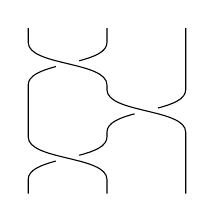
\begin{tikzpicture}[yscale=0.6, baseline=(braid)]
		\braid[style strands={1}, style strands={2}, style strands={3}] (braid) s_1 s_2 s_1;
	\end{tikzpicture}
	\qquad = \qquad
	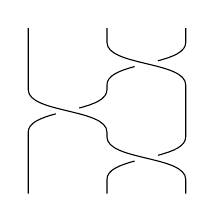
\begin{tikzpicture}[yscale=0.6, baseline=(braid)]
		\braid[style strands={1}, style strands={2}, style strands={3}] (braid) s_2 s_1 s_2;
	\end{tikzpicture} \]

	Dengan cara yang sama, naturalitas kendala komutativitas dapat ditafsirkan secara intuitif sebagai berikut.
	\begin{center}
	$\begin{tikzcd}
		X \otimes Y \arrow[d, "{f \otimes g}"'] \arrow[r, "{c(X, Y)}"] & Y \otimes X \arrow[d, "{g \otimes f}"] \\
		X' \otimes Y' \arrow[r, "{c(X', Y')}"'] & Y' \otimes X'
	\end{tikzcd}$ \quad komutatif ekuivalen dengan \quad
	\begin{tikzpicture}[baseline=(braid),
		midbraid/.style={shape=circle, draw, fill=white, thick, outer sep=0pt, inner sep=0pt, minimum size=5mm} ]
		\coordinate (B1) at (0, 0);
		\coordinate (B2) at (2.2, 0);
		\braid[style strands={1}{lightgray}, style strands={2}{black}, line width=3pt] (bone) at (B1) s_1;
		\node at (bone-1-s) [midbraid, below=3pt] {\small $g$};
		\node at (bone-2-s) [midbraid, below=3pt] {\small $f$};
		\braid[style strands={1}{lightgray}, style strands={2}{black}, line width=3pt] (btwo) at (B2) s_1;
		\node at (btwo-1-e) [midbraid, above=3pt] {\small $g$};
		\node at (btwo-2-e) [midbraid, above=3pt] {\small $f$};
		\node at ($(bone.center)!.5!(btwo.center)$) {$=$};
	\end{tikzpicture}\end{center}
	Karena
	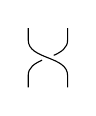
\begin{tikzpicture}[baseline=(braid), scale=0.5]
		\braid[style strands={1}{black}, style strands={2}{black}] (braid) s_1;
	\end{tikzpicture} $\neq$
	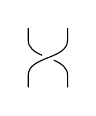
\begin{tikzpicture}[baseline=(braid), scale=0.5]
		\braid[style strands={1}{black}, style strands={2}{black}] (braid) s_1^{-1};
	\end{tikzpicture},
	kategori monoidal $\cate{Braid}$ tidak simetris; sesungguhnya, $c(1, 1)$ membangkitkan grup siklik tak hingga $\mathcal{B}_2 \simeq \Z$, sebagaimana tampak secara intuitif.
\end{example}

Kita telah mengandalkan intuisi topologis untuk memverifikasi semua sifat struktur kepang pada $\cate{Braid}$. Sebaliknya, dapat dibuktikan bahwa segala relasi yang dipenuhi morfisme-morfisme dalam $\cate{Braid}$ terhadap komposisi, yakni berbagai kesamaan diagram kepang, sudah mencakup semua sifat umum kategori monoidal berkepang \cite[Corollary 2.6]{JS93}; dalam ``jargon'' matematikawan, $\cate{Braid}$ adalah ``kategori monoidal berkepang bebas yang dibangkitkan oleh objek $1$''. Dengan kata lain, sifat umum kategori monoidal berkepang dapat diperiksa secara intuitif dalam $\cate{Braid}$. Dibandingkan dengan aksioma-aksioma pada Definisi \ref{def:braiding}, kesamaan antardiagram kepang sering kali langsung terlihat; pembaca kiranya telah menyaksikannya dengan jelas dalam pembahasan persamaan Yang--Baxter.

\section{Kategori Diperkaya}\label{sec:enriched-cat}
Sebenarnya, kita telah menjumpai cukup banyak kategori diperkaya. Kategori diperkaya dapat dipandang dari dua sudut:
\begin{compactitem}
	\item kategori diperkaya merupakan suatu perluasan teori kategori;
	\item kategori diperkaya adalah kategori yang himpunan $\Hom$-nya dilengkapi struktur tambahan.
\end{compactitem}
Sudut pandang pertama memudahkan pengembangan teori dan akan kita gunakan, sedangkan matematikawan biasanya lebih condong pada sudut pandang kedua. Dalam Contoh \ref{eg:categories}, kita telah melihat banyak contohnya; himpunan $\Hom$ dalam kategori-kategori tersebut sering membawa berbagai struktur tambahan, seperti grup abelian atau ruang topologis. Gagasan teori kategori diperkaya ialah
\begin{center}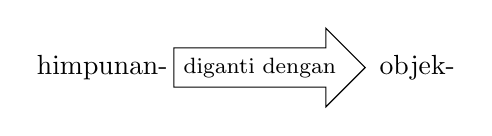
\begin{tikzpicture}
	\node (A) at (0,0) {himpunan-$\Hom$};
	\node (B) at (4,0) {objek-$\Hom$};
	\node[single arrow, draw] at ($(A)!.5!(B)$) {\footnotesize diganti dengan};
\end{tikzpicture}\end{center}
Namun, objek yang disebut terakhir itu merupakan objek dalam kategori apa? Kita harus dapat mendefinisikan komposisi di antara objek-$\Hom$ serta morfisme identitas di dalamnya; kategori monoidal menyediakan bahasa yang sesuai untuk tujuan ini. Monograf mengenai kategori diperkaya dapat dilihat dalam \cite{Ke05}.

\begin{definition}\label{def:enriched-cat}\index{chongshifanchou@kategori diperkaya (enriched category)}
	Misalkan $\mathcal{V}$ kategori monoidal. Yang dimaksud dengan kategori yang diperkaya atas $\mathcal{V}$, atau kategori-$\mathcal{V}$ $\mathcal{C}$, ialah data berikut: \index[sym1]{HomCi@$\iHom_{\mathcal{C}}(X, Y)$}
	\begin{enumerate}
		\item himpunan objek $\Obj(\mathcal{C})$;
		\item untuk setiap dua objek $X, Y \in \Obj(\mathcal{C})$, diberikan objek morfisme $\iHom_{\mathcal{C}}(X, Y) \in \Obj(\mathcal{V})$;
		\item untuk setiap tiga objek $X, Y, Z \in \Obj(\mathcal{C})$, diberikan morfisme komposisi
			\[ M: \iHom_{\mathcal{C}}(Y, Z) \otimes \iHom_{\mathcal{C}}(X, Y) \longrightarrow \iHom_{\mathcal{C}}(X, Z), \]
			seperti biasa, kita akan sering menghilangkan simbol $M$ dan menulis $\iHom_{\mathcal{C}}(\cdots)$ sebagai $\iHom(\cdots)$;
		\item untuk setiap objek $X \in \Obj(\mathcal{C})$, diberikan morfisme identitas
			\[ \identity_X : \munit \to \iHom_{\mathcal{C}}(X ,X); \]
	\end{enumerate}
	sedemikian sehingga diagram-diagram berikut komutatif untuk setiap $X, Y, Z, W \in \Obj(\mathcal{C})$.
	\begin{center} 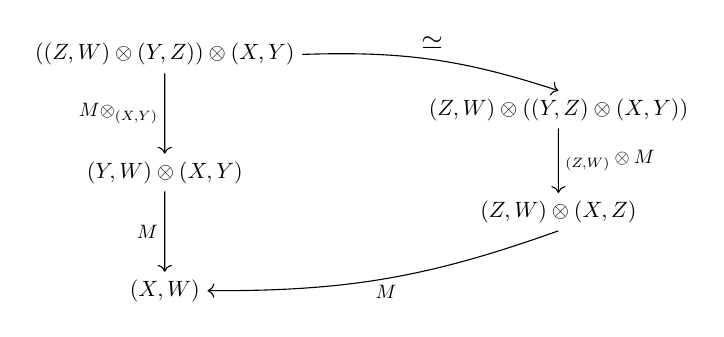
\begin{tikzpicture}[A/.style={scale=0.8, transform shape}, B/.style={scale=0.7, transform shape}, every edge/.style={->, draw}]
		\node[A] (A1) at (0, 3) {$(\iHom(Z, W) \otimes \iHom(Y, Z)) \otimes \iHom(X,Y)$};
		\node[A] (A2) at (0, 1.5) {$\iHom(Y,W) \otimes \iHom(X,Y)$};
		\node[A] (A3) at (0, 0) {$\iHom(X, W)$};
		\node[A] (A4) at (5, 1) {$\iHom(Z,W) \otimes \iHom(X, Z)$};
		\node[A] (A5) at (5, 2.3) {$\iHom(Z,W) \otimes (\iHom(Y,Z) \otimes \iHom(X,Y))$};

		\draw (A1) edge node[B, left] {$M \otimes \identity_{\iHom(X,Y)}$} (A2);
		\draw (A2) edge node[B, left] {$M$} (A3);
		\draw (A4.south) edge[bend left=10] node[B, below] {$M$} (A3.east);
		\draw (A5) edge node[B, right] {$\identity_{\iHom(Z, W)} \otimes M$} (A4);
		\draw (A1.east) edge[bend left=10] node[above]{$\simeq$} (A5.north);
	\end{tikzpicture} \\ \vspace{1.5em}
	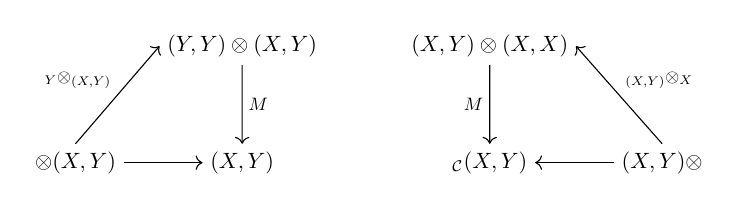
\begin{tikzpicture}[A/.style={scale=0.8, transform shape}, B/.style={auto, scale=0.65, transform shape}, every edge/.style={->, draw}]
		\node[A] (T1) {$\iHom(Y, Y) \otimes \iHom(X,Y)$};
		\node[A] (T2) [below=of T1] {$\iHom(X,Y)$};
		\node[A] (T3) [left=of T2] {$\munit \otimes \iHom(X, Y)$};
		\draw (T3.north) edge node[B] {$\identity_Y \otimes \identity_{\iHom(X,Y)}$} (T1.west);
		\draw (T1) edge node[B] {$M$} (T2);
		\draw (T3) edge (T2);
		
		\node[A] (S1) [right=of T1] {$\iHom(X, Y) \otimes \iHom(X,X)$};
		\node[A] (S2) [below=of S1] {$\iHom_{\mathcal{C}}(X,Y)$};
		\node[A] (S3) [right=of S2] {$\iHom(X, Y) \otimes \munit$};
		\draw (S3.north) edge node[B, swap] {$\identity_{\iHom(X,Y)} \otimes \identity_X$} (S1.east);
		\draw (S1) edge node[B, swap] {$M$} (S2);
		\draw (S3) edge (S2);
	\end{tikzpicture} \end{center}
\end{definition}

Jelas bahwa diagram-diagram komutatif di atas hanyalah versi dalam kategori monoidal dari sifat-sifat morfisme pada Definisi \ref{def:category}. Selanjutnya kita bahas fungtor antarkategori-$\mathcal{V}$. Pembaca mungkin sudah dapat menduganya, tetapi tetap kami uraikan secara lengkap.

\begin{definition}\label{def:enriched-functor}\index{hanzi@fungtor!kasus diperkaya}
	Untuk kategori-$\mathcal{V}$ $\mathcal{C}_1$ dan $\mathcal{C}_2$ yang diberikan, suatu fungtor $F: \mathcal{C}_1 \to \mathcal{C}_2$ ditentukan oleh peta di antara himpunan objek $X \mapsto FX$ dan morfisme antarobjek-$\Hom$, yaitu $\iHom(X, Y) \to \iHom(FX, FY)$, sedemikian sehingga diagram-diagram berikut komutatif untuk semua objek $X, Y, Z$.
	\[ \begin{tikzcd}
		\iHom(Y, Z) \otimes \iHom(X, Y) \arrow[r] \arrow[d] & \iHom(X, Z) \arrow[d] \\
		\iHom(FY, FZ) \otimes \iHom(FX, FY) \arrow[r] & \iHom(FX, FZ)
	\end{tikzcd} \]
	\[ \begin{tikzcd}
		\iHom(X, X) \arrow[rr] & & \iHom(FX, FX) \\
		& \munit \arrow[lu] \arrow[ru] &
	\end{tikzcd} \]
\end{definition}

\begin{remark}\label{rem:enriched-to-ordinary}
	Untuk kategori-$\mathcal{V}$ $\mathcal{C}$, dapat didefinisikan kategori biasa yang bersesuaian sebagai berikut: himpunan objeknya tetap $\Obj(\mathcal{C})$, sedangkan himpunan morfismenya ditetapkan sebagai
	\[ \Hom(X, Y) := \Hom_{\mathcal{V}}\left( \munit, \iHom(X, Y) \right). \]
	Dengan demikian, morfisme identitas $\identity_X: \munit \to \iHom(X, X)$ merupakan unsur $\Hom(X, X)$, dan komposisi morfisme didefinisikan melalui
	\[ \begin{tikzcd}
		\Hom_{\mathcal{V}}\left( \munit, \iHom(Y, Z) \right) \times \Hom_{\mathcal{V}}\left( \munit, \iHom(X, Y) \right) \arrow[d, "{\text{fungtorialitas }\;\otimes}"] \\
		\Hom_{\mathcal{V}}\left( \munit \otimes \munit, \iHom(Y, Z) \otimes \iHom(X, Y) \right) \arrow[d, "{\text{tarik balik melalui }\; \iota: \munit \otimes \munit \rightiso \munit \text{ di atas}}"] \\
		\Hom_{\mathcal{V}}\left( \munit, \iHom(X, Z) \right).
	\end{tikzcd} \]
\end{remark}

\begin{definition}\label{def:enriched-naturaltrans}\index{ziranbianhuan@transformasi natural!kasus diperkaya}
	Misalkan $F, G: \mathcal{C}_1 \to \mathcal{C}_2$ fungtor antarkategori-$\mathcal{V}$. Suatu transformasi natural (atau morfisme) $\theta: F \to G$ ialah keluarga morfisme $\theta_X: \munit \to \iHom(FX, GX)$, dengan $X$ merentang seluruh $\Obj(\mathcal{C}_1)$, sedemikian sehingga diagram berikut komutatif untuk semua $X, Y$.
	\[ \begin{tikzcd}
		\munit \otimes \iHom(X, Y) \arrow[r, "{\theta_Y \otimes F}"] & \iHom(FY, GY) \otimes \iHom(FX, FY) \arrow[d] \\
		\iHom(X, Y) \arrow[u] \arrow[d] & \iHom(FX, GY) \\
		\iHom(X, Y) \otimes \munit \arrow[r, "{G \otimes \theta_X}"'] & \iHom(GX, GY) \otimes \iHom(FX, GX) \arrow[u] .
	\end{tikzcd} \]
\end{definition}
Definisi ini tampak berbelit karena, dalam kategori-$\mathcal{V}$ umum, kita tidak dapat membicarakan unsur-unsur objek-$\Hom$. Definisi komposisi vertikal dan horizontal transformasi natural diserahkan kepada pembaca. Versi diperkaya dari fungtor dan transformasi natural memungkinkan kita mendefinisikan gagasan ekuivalensi kategori bagi kategori-$\mathcal{V}$.\index{fanchoudengjia@ekuivalensi kategori!kasus diperkaya}

\begin{example}
	Ambil $\mathcal{V} = \cate{Set}$ dengan $\otimes := \times$ sehingga menjadi kategori monoidal (Contoh \ref{eg:monoidal-cat}); maka kategori-$\mathcal{V}$ tidak lain adalah kategori yang telah didefinisikan sebelumnya. Perhatikan bahwa kita tetap mengikuti Konvensi \ref{con:U-small}, sehingga $\cate{Set}$ adalah kategori yang terdiri atas himpunan-$\mathcal{U}$ dan kategori berarti kategori-$\mathcal{U}$.
\end{example}

\begin{example}\index{tuopufanchou@kategori topologis (topological category)}
	Serupa dengan itu, ambil $\mathcal{V} = \cate{CGHaus}$ (Contoh \ref{eg:categories}) dan $\otimes := \times$. Kategori diperkaya yang bersesuaian disebut \emph{kategori topologis}. Alasan penggunaan $\cate{CGHaus}$ dapat dilihat dalam pembahasan pada Contoh \ref{eg:categories}, atau dalam \cite[Chapter 5]{May99}. 
\end{example}

\begin{example}\label{eg:Ab-cat}\index{Ab-fanchou@kategori-$\cate{Ab}$}
	Ambil $\mathcal{V} := \cate{Ab}$, dengan $\otimes$ hasil kali tensor grup abelian (yakni modul-$\Z$) dan $\munit := \Z$. Kategori-$\cate{Ab}$ yang diperoleh juga disebut \emph{kategori praaditif}. Sebenarnya, kategori-$\cate{Ab}$ dapat didefinisikan tanpa bahasa kategori monoidal. Pada intinya, ciri-ciri kategori-$\cate{Ab}$ adalah sebagai berikut.
	\begin{compactitem}
		\item Setiap himpunan $\Hom$ dilengkapi struktur grup abelian.
		\item Peta komposisi $\Hom(Y, Z) \times \Hom(X, Y) \to \Hom(X, Z)$ adalah peta $\Z$-bilinear, yakni memenuhi $f(g+h) = fg+ fh$ dan $(g+h)f = gf + hf$. Hal ini karena, menurut sifat hasil kali tensor, homomorfisme grup $\Hom(Y,Z) \dotimes{\Z} \Hom(X, Y) \to \Hom(X, Z)$ sama artinya dengan peta bilinear $\Hom(Y, Z) \times \Hom(X, Y) \to \Hom(X, Z)$.
		\item Dengan menguraikan definisi, terlihat bahwa fungtor antarkategori-$\cate{Ab}$ adalah fungtor yang menginduksi homomorfisme grup pada himpunan-himpunan $\Hom$.
		\item Tidak ada syarat tambahan pada transformasi natural.
	\end{compactitem}
	 Semua ini sesuai dengan sudut pandang yang disebutkan pada awal bagian ini; verifikasi terperinci diserahkan sebagai latihan. Secara khusus, untuk semua objek $X, Y$, dalam $\Hom(X, Y)$ terdapat unsur nol $0$ yang terdefinisi dengan baik, dan komposisinya dengan setiap morfisme yang dapat dikomposisikan tetap merupakan unsur nol. Kategori semacam ini sangat umum: misalnya, untuk sebarang gelanggang $A$, kategori modul kiri $A\dcate{Mod}$ adalah kategori-$\cate{Ab}$, termasuk $\cate{Ab}$ itu sendiri.

	Dalam contoh $\cate{Ab}$, untuk setiap grup abelian $M$ terdapat bijeksi natural
	\begin{align*}
		\Hom_{\cate{Ab}}(\Z, M) & \rightiso M \\
		f & \mapsto f(1),
	\end{align*}
	maka terlihat bahwa fungtor $\Hom_{\cate{Ab}}(\munit, \cdot) = \Hom_{\cate{Ab}}(\Z, \cdot): \cate{Ab} \to \cate{Set}$ isomorfik dengan fungtor pelupa. Karena itu, menerapkan prosedur pada Catatan \ref{rem:enriched-to-ordinary} kepada kategori-$\cate{Ab}$ hanya melupakan struktur grup pada himpunan-himpunan $\Hom$.
\end{example}

Karena kategori-$\cate{Ab}$ sering digunakan dalam matematika, selanjutnya kita kaji beberapa sifat khususnya. Ingat kembali \S\ref{sec:limits}. Jika $I$ himpunan kecil, telah diketahui bahwa dalam kategori $A\dcate{Mod}$ terdapat, dengan $I$ sebagai himpunan indeks, produk $\prod_{i \in I} M_i$ dan koproduk $\bigoplus_{i \in I} M_i$ (yakni jumlah langsung modul). Jika $I$ berhingga, keduanya sama: hal ini langsung terlihat dari definisi konkret $\prod$ dan $\bigoplus$, tetapi juga merupakan fenomena umum yang dimiliki semua kategori-$\cate{Ab}$. Untuk menjelaskannya, kita perkenalkan gagasan biproduk.

\begin{definition}\label{def:biproduct}\index{shuangji@biproduk (biproduct)}
	Misalkan $\mathcal{C}$ kategori-$\cate{Ab}$ dan $X_1, X_2$ objek di dalamnya. \emph{Biproduk} dari $X_1, X_2$ berarti diagram
	\[ \begin{tikzcd}
		X_1 \arrow[r, yshift=-0.5ex, "\iota_1"'] & Z \arrow[l, yshift=0.5ex, "p_1"'] \arrow[r, yshift=0.5ex, "p_2"] & X_2 \arrow[l, yshift=-0.5ex, "\iota_2"]
	\end{tikzcd} \]
	sedemikian sehingga $p_1 \iota_1 = \identity$, $p_2 \iota_2 = \identity$, dan $\iota_1 p_1 + \iota_2 p_2 = \identity_Z$. Kita juga mengatakan bahwa $Z$ bersama $(\iota_1, \iota_2, p_1, p_2)$ adalah biproduk $X_1$ dan $X_2$. Notasinya ialah $Z = X_1 \oplus X_2$.
\end{definition}
Dengan mengomposisikan persamaan $\iota_1 p_1 + \iota_2 p_2 = \identity_Z$ di kiri oleh $p_2$ dan di kanan oleh $\iota_1$, diperoleh $p_2 \iota_1 = 0$; demikian pula diperoleh $p_1 \iota_2 = 0$. Konstruksi biproduk dapat diiterasikan ke kasus banyak peubah $Z = X_1 \oplus \cdots \oplus X_n$: untuk setiap $1 \leq i \leq n$, diberikan $\begin{tikzcd} X_i \arrow[r, yshift=-0.5ex, "\iota_i"'] & Z \arrow[l, yshift=0.5ex, "p_i"'] \end{tikzcd}$ sedemikian sehingga
\begin{gather*}
	p_i \iota_j = \begin{cases} \identity, & i=j \\ 0, & i \neq j \end{cases} \qquad
	\sum_{i=1}^n \iota_i p_i = \identity_Z.
\end{gather*}

\begin{theorem}\label{prop:biproduct-criterion}
	Misalkan $X_1, X_2$ objek dalam kategori-$\cate{Ab}$ $\mathcal{C}$. Pernyataan-pernyataan berikut ekuivalen:
	\begin{compactenum}[(i)]
		\item produk $X _1\times X_2$ ada;
		\item koproduk $X_1 \sqcup X_2$ ada;
		\item biproduk dari $X_1$ dan $X_2$, yaitu $Z$, ada.
	\end{compactenum}
	Jika salah satu pernyataan tersebut berlaku, maka biproduk $Z$ bersama $(p_1, p_2)$ memberikan produk $X_1$ dan $X_2$, sedangkan $Z$ bersama $(\iota_1, \iota_2)$ memberikan koproduknya.
\end{theorem}
Menurut Lema \ref{prop:product-associativity}, produk dan koproduk berhingga dapat dibangun secara iteratif dari kasus biner. Ini menjelaskan mengapa jumlah langsung berhingga modul sekaligus berperan sebagai produk dan koproduk.
\begin{proof}
	Andaikan biproduk dari $X_1, X_2$, yaitu $Z$, ada. Karena
	\begin{align*}
		p_1 \iota_2 & = p_1 \circ \identity_Z \circ \iota_2 =  p_1 (\iota_1 p_1 + \iota_2 p_2) \iota_2 = (p_1 \iota_1) p_1 \iota_2 + p_1 \iota_2 (p_2 \iota_2)  \\
		& = p_1 \iota_2 + p_1 \iota_2,
	\end{align*}
	maka $p_1 \iota_2 = 0$. Demikian pula, $p_2 \iota_1 = 0$. Untuk morfisme-morfisme yang diberikan $X_1 \xleftarrow{f_1} W \xrightarrow{f_2} X_2$, tetapkan $\phi := \iota_1 f_1 + \iota_2 f_2 : W \to Z$. Dari rumus sebelumnya diperoleh $p_i \phi = f_i$ ($i=1,2$). Sebaliknya, jika $\phi: W \to Z$ memenuhi $p_i \phi = f_i$, maka
	\[ \phi = (\iota_1 p_1 + \iota_2 p_2) \phi = \iota_1 f_1 + \iota_2 f_2 \]
	menentukan $\phi$ secara tunggal. Jadi, $(Z, p_1, p_2)$ memang memenuhi sifat universal produk.

	Sekarang andaikan $X_1 \xleftarrow{p_1} Z \xrightarrow{p_2} X_2$ adalah produk. Untuk $i=1,2$, definisikan $\iota_i: X_i \to Z$ sedemikian sehingga
	\[ \forall j=1,2, \quad  p_j \iota_i =
		\begin{cases}
			\identity_{X_i}, & i=j, \\
			0, & i \neq j .
		\end{cases}
	\]
	Cukup diverifikasi $\iota_1 p_1 + \iota_2 p_2 = \identity_Z$ untuk membuktikan bahwa $(Z, \iota_1, \iota_2, p_1, p_2)$ adalah biproduk. Kita mempunyai
	\begin{align*}
		p_1 (\iota_1 p_1 + \iota_2 p_2) & = p_1 + 0 = p_1 \circ \identity_Z , \\
		p_2 (\iota_1 p_1 + \iota_2 p_2) & = 0 + p_2 = p_2 \circ \identity_Z.
	\end{align*}
	Dari sifat universal produk diperoleh $\iota_1 p_1 + \iota_2 p_2 = \identity_Z$. Kasus koproduk diperoleh dengan membalik arah panah.
\end{proof}
\begin{remark}
	Dengan mencermati pembuktian, terlihat bahwa isomorfisme $\psi: X_1 \sqcup X_2 \rightiso X_1 \times X_2$ dapat dipilih sebagai morfisme yang dicirikan oleh
	\[ p_j \psi \iota_i =
		\begin{cases}
			\identity_{X_i}, & i=j, \\
			0, & i \neq j
		\end{cases} \]
	dengan $\iota_i : X_i \to X_1 \sqcup X_2$ dan $p_i: X_1 \times X_2 \to X_i$.
\end{remark}

\begin{lemma}
	Misalkan $X$ objek dalam kategori-$\cate{Ab}$ $\mathcal{C}$. Sifat-sifat berikut ekuivalen:
	\begin{compactenum}[(i)]
		\item $X$ adalah objek awal,
		\item $\identity_X = 0$,
		\item $\End_{\mathcal{C}}(X) = \{0\}$,
		\item $X$ adalah objek terminal.
	\end{compactenum}
	Secara khusus, jika $X$ objek awal atau objek terminal, maka $X$ adalah objek nol (Definisi \ref{def:universal-objects}), dan $0 \in \Hom(X, \cdot)$ adalah morfisme nol pada Definisi \ref{def:zero-morphism}.
\end{lemma}
\begin{proof}
	Andaikan $X$ objek awal dalam $\mathcal{C}$. Grup $\End_{\mathcal{C}}(X)$ hanya mempunyai satu unsur, yang haruslah $0 = \identity_X$; jadi (i) $\implies$ (ii). Karena untuk setiap $Y$ dan $f \in \Hom(X, Y)$ berlaku $f \circ \identity_X = f$, sifat kategori-$\cate{Ab}$ memberikan (ii) $\implies$ (iii) $\implies$ (i). Dengan membalik arah panah, terlihat bahwa (iv) ekuivalen dengan syarat-syarat lainnya.
\end{proof}

\begin{definition}[Fungtor Aditif dan Kategori Aditif]\label{def:additive-cat}\index{jiaxingfanchou@kategori aditif (additive category)}\index{hanzi@fungtor!kasus aditif}
	Fungtor antarkategori-$\cate{Ab}$ (lihat Definisi \ref{def:enriched-functor}) disebut \emph{fungtor aditif}. Jika kategori-$\cate{Ab}$ $\mathcal{C}$ mempunyai objek nol $0$ dan setiap $X, Y \in \Obj(\mathcal{C})$ mempunyai biproduk $X \oplus Y$, maka $\mathcal{C}$ disebut \emph{kategori aditif}. 
\end{definition}

Kategori modul $A\dcate{Mod}$ yang telah disebutkan sebelumnya adalah contoh khas kategori aditif; lihat Korolari \ref{prop:Mod-cat-additive}. Fungtor $F: \mathcal{C}_1 \to \mathcal{C}_2$ adalah fungtor aditif jika dan hanya jika $\Hom_{\mathcal{C}_1}(X, Y) \to \Hom_{\mathcal{C}_2}(FX, FY)$ merupakan homomorfisme grup aditif untuk setiap $X, Y$.

\begin{proposition}\label{prop:biproduct-preservation}
	Fungtor aditif antarkategori-$\cate{Ab}$ mempertahankan biproduk.
\end{proposition}
\begin{proof}
	Jika $F: \mathcal{C} \to \mathcal{C}'$ fungtor aditif dan data $(\iota_1, \iota_2, p_1, p_2)$ mendefinisikan biproduk dalam $\mathcal{C}$, maka data $(F(\iota_1), F(\iota_2), F(p_1), F(p_2))$ tetap memenuhi syarat-syarat biproduk. Alasannya, biproduk didefinisikan oleh persamaan, bukan oleh keberadaan panah.
\end{proof}

\begin{proposition}\label{prop:additive-prod-coprod}
	Dalam kategori aditif, produk dan koproduk sebarang keluarga berhingga objek ada dan keduanya isomorfik secara natural.
\end{proposition}
\begin{proof}
	Kasus dua objek tidak lain adalah Teorema \ref{prop:biproduct-criterion} tentang biproduk; kasus umum direduksi ke kasus dua objek melalui kendala asosiativitas pada Lema \ref{prop:product-associativity}.
\end{proof}

\section{Sekilas tentang \texorpdfstring{$2$}{2}-Kategori}\label{sec:2-cat}
Kita telah terbiasa menggambarkan objek suatu kategori sebagai titik dan morfismenya sebagai panah di antara titik-titik tersebut; konstruksi berdimensi tertinggi dalam gambaran ini adalah panah satu dimensi, sehingga kategori wajar disebut $1$-kategori. Kategori yang diperoleh dengan melupakan panah tidak lain adalah himpunan: yang tersisa hanya objek berdimensi nol, sehingga himpunan dapat dipandang sebagai $0$-kategori. Ini menimbulkan pertanyaan yang wajar: bagaimana kategori tingkat lebih tinggi didefinisikan? Bagian ini hanya membahas tingkat $2$; dengan kata lain, selain titik dan panah kita akan menambahkan konstruksi berdimensi $2$ tertentu, yang disebut $2$-sel.

$2$-Kategori bukan khayalan tanpa dasar. Sebagai contoh, $\cate{Cat}$ dalam Contoh \ref{eg:Cat} merupakan contoh baku; contoh alami lainnya diperoleh dengan meninjau ruang topologis (titik), peta kontinu di antaranya (panah), dan homotopi antarpeta ($2$-sel). Meskipun gagasannya sederhana, menyarikan definisi yang tepat merupakan persoalan besar. Versi definisi berikut juga disebut $2$-kategori ketat.

\begin{definition}\index{$2$-kategori}
	Suatu $2$-kategori (ketat) $\mathcal{C}$ terdiri atas data berikut:
	\begin{itemize}
		\item himpunan objek, yang juga disebut $0$-morfisme, $\Obj(\mathcal{C}) = \Mor_0(\mathcal{C})$;
		\item himpunan $1$-morfisme, $\Mor_1(\mathcal{C}) = \bigsqcup_{X, Y \in \Mor_0(\mathcal{C})} \Hom(X, Y)$;
		\item himpunan $2$-morfisme, $\Mor_2(\mathcal{C}) = \bigsqcup_{a, b \in \Mor_1(\mathcal{C})} \Hom(a, b)$.
	\end{itemize}
	Biasanya $1$-morfisme ditulis dalam bentuk $f: X \to Y$, sedangkan $2$-morfisme ditulis dalam bentuk $\theta: a \Rightarrow b$. Di dalam $\mathcal{C}$ terdapat operasi-operasi berikut.
	\begin{enumerate}[(i)]
		\item Kita mensyaratkan bahwa objek-objek $\mathcal{C}$ beserta $1$-morfismenya membentuk suatu kategori ($1$-kategori).
		% Komposisi $1$-morfisme $\Hom(Y, Z) \times \Hom(X, Y) \to \Hom(X, Z)$, dengan $X, Y, Z$ objek; di sini komposisi disyaratkan memenuhi hukum asosiatif, dan untuk setiap objek $X$ terdapat unsur identitas $\identity_X$. Dengan kata lain, objek $\mathcal{C}$ beserta $1$-morfismenya disyaratkan membentuk suatu kategori.
		\item $2$-Morfisme mempunyai dua macam komposisi, yaitu vertikal dan horizontal. Pertama-tama tinjau komposisi vertikal: misalkan $X, Y$ objek, $f, g, h: X \to Y$ merupakan $1$-morfisme, serta $\theta: f \Rightarrow g$ dan $\psi: g \Rightarrow h$ merupakan $2$-morfisme. Maka terdapat komposisi vertikal $\psi \circ \theta: f \Rightarrow h$, yang digambarkan sebagai
			\[ \begin{tikzcd}
				X
				\arrow[bend left=60, rr, "f", ""' name=U]
				\arrow[rr, "g"' name=M, "" name=MM]
				\arrow[bend right=60, rr, "" name=D, "h"'] & &
				\arrow[Rightarrow, to path=(U) -- (MM) \tikztonodes, "\theta"] \arrow[Rightarrow, to path=  (M) -- (D) \tikztonodes, "\psi"]  Y
			\end{tikzcd}
			\quad \text{dikomposisikan menjadi} \quad
			\begin{tikzcd}
				X
				\arrow[bend left=50, rr, "f", ""' name=U]
				\arrow[bend right=50, rr, "" name=D, "h"']
				& & \arrow[Rightarrow, to path=(U) -- (D) \tikztonodes, "\psi \circ \theta"] Y .
			\end{tikzcd} \]
		\item Selanjutnya tinjau komposisi horizontal. Misalkan $X, Y ,Z$ objek, \begin{tikzcd} X \arrow[r, bend left=20, "f"] \arrow[r, bend right=20, "g"'] & Y \end{tikzcd}, \begin{tikzcd} Y \arrow[r, bend left=20, "f'"] \arrow[r, bend right=20, "g'"'] & Z \end{tikzcd} merupakan dua pasang $1$-morfisme, sedangkan $\theta: f \Rightarrow g$ dan $\psi: f' \Rightarrow g'$ merupakan $2$-morfisme. Maka terdapat komposisi horizontal $\psi \circ \theta: f'f \Rightarrow g'g$, yang digambarkan sebagai
			\[ \begin{tikzcd}
				X \arrow[bend left=50, r, "f", ""' name=LU] \arrow[bend right=50, r, "" name=LD, "g"'] &
				Y \arrow[bend left=50, r, "f'", ""' name=RU] \arrow[bend right=50, r, "" name=RD, "{g'}"'] &
				\arrow[Rightarrow, to path=(LU) -- (LD) \tikztonodes, "\theta"] \arrow[Rightarrow, to path=(RU) -- (RD) \tikztonodes, "\psi"] Z
			\end{tikzcd}
			\quad \text{dikomposisikan menjadi} \quad
			\begin{tikzcd}
				X
				\arrow[bend left=40]{rr}{f'f}[name=U, below]{}
				\arrow[bend right=40]{rr}[name=D]{}[below]{g'g}
				& & \arrow[Rightarrow, to path=(U) -- (D) \tikztonodes]{}{\psi \circ \theta} Z .
			\end{tikzcd} \]
	\item Diagram berbentuk
		\begin{tikzcd}
			X
			\arrow[bend left=30]{rr}{f}[name=U, below]{}
			\arrow[bend right=30]{rr}[name=D]{}[below]{g}
			& & \arrow[Rightarrow, to path=(U) -- (D) \tikztonodes]{}{\theta} Y
		\end{tikzcd}
		disebut $2$-sel. Kita mensyaratkan agar komposisi horizontal memenuhi hukum asosiatif secara ketat, $\phi \circ (\psi \circ \theta) = (\phi \circ \psi) \circ \theta$, dan agar untuk setiap objek $X$ terdapat identitas horizontal (atau sebaiknya disebut sel identitas horizontal) $\identity_{X, 2}: \identity_X \Rightarrow \identity_X$, sedemikian sehingga $\theta \circ \identity_{X, 2} = \theta$ dan $\identity_{X, 2} \circ \psi = \psi$ setiap kali komposisi horizontal tersebut terdefinisi.
	\item Demikian pula, komposisi vertikal $2$-sel disyaratkan memenuhi hukum asosiatif secara ketat, dan untuk setiap $1$-morfisme $f$ terdapat identitas vertikal $\identity_f: f \Rightarrow f$.
	\item Komposisi horizontal dari identitas-identitas vertikal tetap merupakan identitas vertikal:
		\[ \begin{tikzcd}
		X \arrow[bend left=50, r, "f", ""' name=LU] \arrow[bend right=50, r, "" name=LD, "f"'] &
		Y \arrow[bend left=50, r, "{f'}", ""' name=RU] \arrow[bend right=50, r, "" name=RD, "{f'}"'] &
		\arrow[Rightarrow, to path=(LU) -- (LD) \tikztonodes, "{\identity_f}"] \arrow[Rightarrow, to path=(RU) -- (RD) \tikztonodes, "{\identity_{f'}}"]  Z
	\end{tikzcd}
	\quad \text{komposisi horizontalnya adalah} \quad
	\begin{tikzcd}
		X
		\arrow[bend left=40, rr, "{f'f}", ""' name=U]
		\arrow[bend right=40, rr, "{f'f}"', "" name=D]
		& & \arrow[Rightarrow, to path=(U) -- (D) \tikztonodes, "{\identity_{f'f}}"] Z .
	\end{tikzcd} \]
	\item Komposisi vertikal dan horizontal memenuhi hukum pertukaran: untuk diagram
		\[ \begin{tikzcd}
			X
			\arrow[bend left=60, rr, ""' name=U]
			\arrow[rr, "" name=MM, ""' name=M]
			\arrow[bend right=60, rr, "" name=D] & &
			\arrow[Rightarrow, to path=(U) -- (MM) \tikztonodes, "\theta"] \arrow[Rightarrow, to path=  (M) -- (D) \tikztonodes, "\psi"] Y
			\arrow[bend left=60, rr, ""' name=V]
			\arrow[rr, "" name=NN, ""' name=N]
			\arrow[bend right=60, rr, "" name=E] & &
			\arrow[Rightarrow, to path=(V) -- (NN) \tikztonodes, "\theta'"] \arrow[Rightarrow, to path=  (N) -- (E) \tikztonodes, "\psi'"] Z
		\end{tikzcd} \]
		berlaku
		\[ \left( \psi' \underset{\text{vertikal}}{\circ} \theta'\right) \underset{\text{horizontal}}{\circ} \left( \psi \underset{\text{vertikal}}{\circ} \theta\right) = \left( \psi' \underset{\text{horizontal}}{\circ} \psi \right) \underset{\text{vertikal}}{\circ} \left( \theta' \underset{\text{horizontal}}{\circ} \theta\right).  \]
	\end{enumerate}
\end{definition}

\begin{remark}
	Definisi di atas jelas bertentangan dengan semangat Catatan \ref{rem:strict-or-not}, sebab komposisi morfisme kita syaratkan memenuhi hukum asosiatif dan sifat identitas secara ketat. Untuk $2$-kategori terdapat versi definisi yang lebih longgar sekaligus jauh lebih rumit, misalnya bikategori; untungnya, bikategori juga memenuhi teorema koherensi, yakni setiap bikategori ekuivalen dengan suatu $2$-kategori (bandingkan dengan definisi kategori monoidal dan teorema koherensinya \ref{prop:ML-coherence}). Fenomena koherensi semacam ini tidak lagi berlaku bagi kategori bertingkat lebih dari $2$. Karena keterbatasan ruang, pembahasan kita cukupkan sampai di sini.
\end{remark}

\begin{example}\label{eg:Cat}\index[sym1]{Cat@$\cate{Cat}$}
	Contoh khas $2$-kategori ialah $\cate{Cat}$, yang untuk sementara dapat dibayangkan secara kasar sebagai ``kategori dari kategori-kategori''; bayangan naif semacam itu segera menghadapi kesulitan teori himpunan. Di sini kita harus memilih suatu semesta Grothendieck $\mathcal{U}$ dan, sesuai Konvensi \ref{con:U-small}, membedakan kategori dari kategori kecil. Sekarang $2$-kategori $\cate{Cat}$ dapat didefinisikan sebagai berikut.
	\begin{compactitem}
		\item Objek atau $0$-morfisme: himpunan semua kategori kecil.
		\item $1$-Morfisme: $\Hom(\mathcal{C}_1, \mathcal{C}_2)$ didefinisikan sebagai himpunan fungtor dari $\mathcal{C}_1$ ke $\mathcal{C}_2$.
		\item $2$-Morfisme: $\Hom(\alpha, \beta)$ didefinisikan sebagai himpunan transformasi natural $\theta: \alpha \to \beta$.
		\item Komposisi $1$-morfisme didefinisikan sebagai komposisi fungtor; komposisi vertikal dan horizontal $2$-morfisme masing-masing didefinisikan sebagai komposisi vertikal dan horizontal transformasi natural.
	\end{compactitem}
	Definisi identitas vertikal dan horizontal sudah jelas sehingga tidak perlu diuraikan lagi. Lema \ref{prop:naturaltrans-associativity} memastikan bahwa $\cate{Cat}$ memenuhi aksioma-aksioma $2$-kategori.
\end{example}

Jika pada $\cate{Cat}$ kita melupakan $2$-morfismenya dan hanya meninjau struktur kategori biasa yang dimilikinya, maka $\cate{Cat}$ mempunyai struktur monoidal alami: operasi $\otimes$ diambil sebagai produk kategori $\times$, sedangkan objek satuannya $\munit$ adalah kategori yang hanya mempunyai satu morfisme (ingat Contoh \ref{eg:categories}). Perhatikan bahwa $\times$ dapat dipahami sebagai produk dalam kategori $\cate{Cat}$, sedangkan $\munit$ merupakan objek terminal $\cate{Cat}$; karena itu, konstruksi ini adalah kasus khusus dari Contoh \ref{eg:monoidal-cat}.

\begin{remark}
	Sekarang $2$-kategori dapat dipahami melalui gagasan kategori diperkaya. Misalkan $\mathcal{C}$ suatu $2$-kategori. Untuk setiap objek $X, Y$, definisikan kategori vertikal $\mathcal{V}(X, Y)$ yang objeknya merupakan $1$-morfisme $f: X \to Y$ dan morfismenya merupakan $2$-morfisme $\theta: f \Rightarrow g$; komposisi morfisme diberikan oleh komposisi vertikal $2$-morfisme. Hukum asosiatif vertikal serta sifat identitas vertikal $\identity_f: f \Rightarrow f$ memastikan bahwa $\mathcal{V}(X, Y)$ memang suatu kategori. Selanjutnya kita andaikan bahwa setiap $\mathcal{V}(X, Y)$ merupakan kategori kecil. Untuk $\cate{Cat}$, kategori vertikal $\mathcal{V}(\mathcal{C}_1, \mathcal{C}_2)$ yang bersesuaian tidak lain adalah kategori fungtor $\text{Fct}(\mathcal{C}_1, \mathcal{C}_2)$ yang didefinisikan pada \S\ref{sec:functor-category}.

	Struktur $2$-kategori $\mathcal{C}$ dapat dirumuskan kembali sebagai berikut:
	\begin{compactitem}
		\item himpunan objek $\Obj(\mathcal{C})$;
		\item untuk setiap $X, Y \in \Obj(\mathcal{C})$, diberikan suatu kategori $\mathcal{V}(X, Y)$;
		\item untuk setiap $X, Y, Z \in \Obj(\mathcal{C})$, diberikan fungtor biner
			\[ \circ: \mathcal{V}(Y, Z) \times \mathcal{V}(X, Y) \to \mathcal{V}(X, Z); \]
		\item untuk setiap $X \in \Obj(\mathcal{C})$, diberikan fungtor
			\[ U_X: \munit \to \mathcal{V}(X, X); \]
		\item kita mensyaratkan agar fungtor $\circ$ memenuhi hukum asosiatif secara ketat dan agar $U_X$ mempunyai sifat unsur identitas terhadap $\circ$.
	\end{compactitem}
	Sesungguhnya, pada tataran objeknya, fungtor $\circ: \mathcal{V}(Y, Z) \times \mathcal{V}(X, Y) \to \mathcal{V}(X, Z)$ memuat operasi komposisi $1$-morfisme; pada tataran morfismenya, fungtor tersebut memuat operasi komposisi horizontal $2$-morfisme. Dapat diperiksa bahwa fungtor itu sekaligus memuat sifat identitas horizontal dan hukum pertukaran dalam definisi $2$-kategori. Memilih fungtor $U_X: \munit \to \mathcal{V}(X, X)$ setara dengan menandai suatu objek dalam $\Hom(X, X)$, dan objek itu tidak lain adalah $\identity_X$.

	Ringkasnya, $2$-kategori tidak lain adalah kategori yang diperkaya atas $\cate{Cat}$: untuk setiap objek $X, Y \in \Obj(\mathcal{C})$, himpunan-$\Hom$ $\Hom(X, Y)$ kita perkaya menjadi kategori vertikal $\iHom(X, Y) := \mathcal{V}(X, Y)$, yang merupakan objek kategori monoidal $\cate{Cat}$. Dengan demikian, kita sampai pada Definisi \ref{def:enriched-cat} tentang kategori diperkaya.
\end{remark}

\begin{definition}
	$2$-Fungtor dan $2$-transformasi natural di antara $2$-kategori didefinisikan menurut konstruksi kategori yang diperkaya atas $\cate{Cat}$ (lihat Definisi \ref{def:enriched-functor}, \ref{def:enriched-naturaltrans}).
\end{definition}
Pembaca dipersilakan mencoba menguraikan definisi-definisi tersebut. Sebagai contoh, definisi $2$-fungtor memetakan $i$-morfisme ke $i$-morfisme (di sini $i=0,1,2$) dan mempertahankan sumber/target, komposisi, identitas, serta sifat-sifat lain dari morfisme tersebut.

\begin{convention}
	Untuk $2$-kategori, kita tetap menggunakan beberapa diagram yang diperkenalkan ketika membahas transformasi natural (yakni $2$-kategori $\cate{Cat}$), misalnya diagram dalam \S\ref{sec:functors} yang berbentuk
	\[ \begin{tikzcd}
		X \arrow[r, "h"] & Y \arrow[bend left=50, r, "f", ""' name=U] \arrow[bend right=50, r, "" name=D, "g"'] & Z \arrow[Rightarrow, to path=(U)--(D) \tikztonodes, "\theta"] \arrow[r, "k"] & W
	\end{tikzcd} \]
	yang komposisi horizontalnya bermakna bahwa masing-masing $1$-morfisme $h, k$ ``dilebarkan'' menjadi $2$-sel $\identity_h, \identity_k$, lalu komposisi horizontal dilakukan. Demikian pula, diagram yang diperkenalkan dalam Catatan \ref{rem:triangle-identity},
	\[\begin{tikzcd}
		{} & X \arrow[rr, "\identity", ""' name=I] \arrow[rd, "f"] \arrow[Rightarrow, d, "\varepsilon"] & & X \\
		Y \arrow[ru, "g"] \arrow[rr, "" name=J, "\identity"'] & {} & Y \arrow[ru, "g"'] \arrow[Leftarrow, to path= -- (I) \tikztonodes, "\eta"] &
	\end{tikzcd} \]
	menyatakan komposisi berikut dalam $2$-kategori:
	\[ \begin{tikzcd}
		Y \arrow[r, "g"] \arrow[bend right=60, rr, "" name=J, "\identity"'] &
		X \arrow[r, "f"] \arrow[bend left=60, rr, "\identity", ""' name=I] \arrow[Rightarrow, to path= --(J) \tikztonodes, "\varepsilon"] &
		Y \arrow[r, "g"] \arrow[Leftarrow, to path= -- (I) \tikztonodes, "\eta"] &
		X .
	\end{tikzcd} \]
\end{convention}

\begin{remark}\index{bansuidui@pasangan adjoin}
	Pasangan adjoin $(F, G, \eta, \varepsilon)$ yang dibahas dalam \S\ref{sec:adjoint-functor} dapat dirumuskan kembali dengan bahasa $2$-kategori. Misalkan
	\[\begin{tikzcd}
		X \arrow[yshift=0.5ex, r, "f"] & Y \arrow[yshift=-0.5ex, l, "g"]
	\end{tikzcd}\]
	di dalam suatu $2$-kategori $\mathcal{C}$ merupakan sepasang $1$-morfisme, sedangkan $\eta: \identity_X \Rightarrow gf$ dan $\varepsilon: fg \Rightarrow \identity_Y$ merupakan $2$-morfisme. Jika keduanya memenuhi identitas segitiga dalam Catatan \ref{rem:triangle-identity}, maka $(f, g, \eta, \varepsilon)$ disebut pasangan adjoin. Dengan mengambil $\mathcal{C} = \cate{Cat}$, kita memperoleh kembali definisi klasik pasangan adjoin. Banyak sifat fungtor adjoin dapat diperluas ke kasus $2$-kategori; misalnya, pembuktian Teorema Ekuivalensi Adjoin \ref{prop:adjoint-equivalence} dapat digunakan tanpa perubahan.
\end{remark}
	
\begin{Exercises}
	\item 对于一般幺半范畴中的对象 $X_1, \ldots, X_{n+1}$, 有种种方式能构作循序的 $n$-重 $\otimes$ 运算, 取决于安插括号的方法, 如 $\cdots \otimes (X_i \otimes X_{i+1}) \cdots$ 等等. 证明括号的放法恰有 $\frac{1}{n+1} \binom{2n}{n}$ 种. \begin{hint} 此即组合学中的 Catalan 数. \end{hint}
	\item 证明对任意幺半范畴, $\End(\munit)$ 对态射的合成交换. \begin{hint} 应用引理 \ref{prop:Kelly} 和 $(f \otimes \identity)(\identity \otimes g) = f \otimes g = (\identity \otimes g) (f \otimes \identity)$.\end{hint}
	\item 考虑全体有限全序集和保序映射所成范畴 $\cate{On}_f$. 对于有限全序集 $\sigma$, $\tau$, 在 $\sigma \sqcup \tau$ 上定义唯一的全序使得 $\sigma$ 和 $\tau$ 到 $\sigma \sqcup \tau$ 的嵌入是保序的, 而且 $\sigma$ 中的元素总小于 $\tau$ 中元素. 证明 $\sqcup$ 赋予 $\cate{On}_f$ 自然的幺半范畴结构, 其幺元是空集.
	\item 承上, 说明存在唯一的同构 $c(\sigma, \tau): \sigma \sqcup \tau \rightiso \tau \sqcup \sigma$, 证明 $(\cate{On}_f, \sqcup, c)$ 构成对称幺半范畴.
	\item 本题假定读者熟悉向量空间的张量积. 令 $V$ 为域 $\Bbbk$ 上的向量空间, $R$ 为 $V \otimes V$ 的线性自同构, 相应的杨--Baxter 方程定义作
		\[ (R \otimes \identity_V) \, (\identity_V \otimes R) \, (R \otimes \identity_V) = (\identity_V \otimes R) \, (R \otimes \identity_V) \, (\identity_V \otimes R) , \]
		其中每一项都是 $V \otimes V \otimes V$ 的线性自同构. 设 $\{e_i\}_{i \in I}$ 是 $V$ 的基, 将 $R$ 按 $R(e_i \otimes e_j) = \sum_{k,l} R^{k,l}_{i,j} e_k \otimes e_l$ 展开, 那么上述方程化作
		\[ \forall i,j,k,l,m,n, \quad \sum_{p,q,y} R^{p,q}_{i,j} R^{y,n}_{q,k} R^{l,m}_{p,y} = \sum_{y,q,r} R^{q,r}_{j,k} R^{l,y}_{i,q} R^{m,n}_{y,r}.  \]
		显然此方程不易求解. 如果 $\mathcal{V}$ 是 $(\cate{Vect}(\Bbbk), \otimes, \ldots)$ 的一个幺半子范畴, 且具有辫结构 $c$, 那么对任意 $V \in \Obj(\mathcal{V})$, 从 $R := c(V,V)$ 可得出杨--Baxter 方程的解. 这些方程和一些量子可积系统密切相关. 这也解释了命题 \ref{prop:YBE-cat-strict} 的背景. 请验证上述论断.
		
		现在引进参数 $q \in \Bbbk^\times$. 对于有限维 $\Bbbk$-向量空间 $V = \bigoplus_{i=1}^h \Bbbk e_i$, 证明
		\[ R(e_i \otimes e_j) = \begin{cases}
			e_j \otimes e_i, & i < j, \\
			q e_i \otimes e_j, & i = j, \\
			e_j \otimes e_i + (q - q^{-1}) e_i \otimes e_j, & i > j
		\end{cases} \]
		给出杨--Baxter 方程的解, 并且满足 $\left( R - q \cdot \identity_{V \otimes V} \right) \left( R + q^{-1} \cdot \identity_{V \otimes V} \right) = 0$. 当 $q=1$ 时它退化为 $\cate{Vect}(\Bbbk)$ 上标准的辫结构 $v \otimes w \mapsto w \otimes v$. \index{YBE}

	\item 设 $(\mathcal{V}, \otimes, \ldots)$ 为幺半范畴. 为简便起见, 以下设其为严格幺半范畴, 省略结合约束等态射和括号. 定义幺半范畴 $Z(\mathcal{V})$ 使得:
		\begin{itemize}
			\item 其对象为 $(X, \Phi)$, 其中 $X$ 是 $\mathcal{V}$ 的对象而 $\Phi: (X \otimes -) \rightiso (- \otimes X)$ 是函子的同构, 我们进一步要求对所有对象 $Y,Z$, 下图交换.
				\[\begin{tikzcd}[column sep=small]
					X \otimes Y \otimes Z \arrow[rr, "\Phi_{Y \otimes Z}"] \arrow[rd, "{\Phi_Y \otimes \identity_Z}"'] & & Y \otimes Z \otimes X \\
					&  Y \otimes X \otimes Z \arrow[ru, "{\identity_Y \otimes \Phi_Z}"'] &
				\end{tikzcd}\]
			\item 从 $(X, \Phi)$ 到 $(Y, \Psi)$ 的态射取为所有满足下式的 $f \in \Hom_{\mathcal{V}}(X,Y)$
				\[ \forall Z \in \Obj(\mathcal{V}),\quad (\identity_Z \otimes f) \Phi_Z = \Psi_Z (f \otimes \identity_Z) \; \in \Hom_{\mathcal{V}}(X \otimes Z, Z \otimes Y); \]
			\item 取 $(X, \Phi) \otimes (Y, \Psi)$ 为 $(X \otimes Y,\; (\Phi \otimes \identity)(\identity \otimes \Psi))$. 定义 $Z(\mathcal{V})$ 之幺元为 $\left(\munit, (\identity_X)_{X \in \Obj(\mathcal{V})}\right)$.
		\end{itemize}
		验证这确实给出幺半范畴. 此外 $Z(\mathcal{V})$ 具有自然的辫结构, 试阐明之. 范畴 $Z(\mathcal{V})$ 称为 $\mathcal{V}$ 的 Drinfeld 中心, 这是幺半群中心的一种范畴化.
	\item 验证例 \ref{eg:Ab-cat} 中 $\cate{Ab}$-范畴的刻画确实符合充实范畴的一般理论.
	\item 对给定的函子 $\mathcal{A} \xrightarrow{S} \mathcal{C} \xleftarrow{T} \mathcal{B}$, 按定义 \ref{def:comma-category} 构造范畴 $(S/T)$ (回忆其对象形如 $(A,B,f)$) 及投影函子 $P,Q$. 定义态射 $\alpha: SP \to TQ$ 为 $SP(A,B,f) = \left[ SA \xrightarrow{f} TB \right] = TQ(A,B,f)$. 证明 $\alpha$ 确实是函子间的态射, 而且
		\[\begin{tikzcd}
			(S/T) \arrow[r, "P"] \arrow[d, "Q"'] & \mathcal{A} \arrow[d, "S"] \arrow[Rightarrow, ld, "\alpha" description] \\
			\mathcal{B} \arrow[r, "T"'] & \mathcal{C}
		\end{tikzcd}\]
		是 $2$-范畴 $\cate{Cat}$ 中的 $2$-胞腔.
\end{Exercises}

	% Sumber LaTeX untuk buku ``Metode Aljabar'' dalam bahasa Tionghoa
% Hak cipta 2018 Wen-Wei Li.
% Izin diberikan untuk menyalin, menyebarluaskan, dan/atau mengubah
% dokumen ini berdasarkan ketentuan Creative Commons
% Attribution 4.0 International (CC BY 4.0)
% http://creativecommons.org/licenses/by/4.0/
% Terjemahan Bahasa Indonesia: OpenAI Codex gpt-5.6-sol, Ultra, atas instruksi pengguna.
% Terjemahan independen ini tidak menyiratkan dukungan penulis atau sumber manusia mana pun.

% Untuk disertakan
\chapter{Teori Grup}
Grup merupakan salah satu struktur paling mendasar dalam aljabar. Pokok bahasan bab ini secara garis besar terbagi menjadi dua jenis:
\begin{compactenum}
	\item konstruksi formal, yang mencakup definisi dasar semigrup, monoid, dan grup, serta konsep-konsep seperti aksi grup, produk langsung, dan grup bebas; semuanya juga menjadi landasan untuk mempelajari struktur aljabar lainnya;
	\item sifat-sifat konkret grup itu sendiri, terutama dari sudut pandang kombinatorial, yang mencakup tiga teorema Sylow untuk grup berhingga, grup simetris, serta presentasi grup kepang. Bagian ini kaya akan teknik dan merupakan salah satu daya tarik teori grup.
\end{compactenum}
Kami berupaya merajut kedua jenis bahasan tersebut secara berselang-seling. Untuk konsep dasar teori grup, buku ini tidak memberikan uraian pembedaan yang berkepanjangan. Namun, sifat-sifat formal dan beberapa konstruksi penting yang kerap terlewat dalam buku teks dasar---misalnya grup bebas dan kompletisasi---dibahas secara terperinci sebagai persiapan bagi bab-bab selanjutnya. Adapun pada sisi konkret teori grup, grup simetris merupakan salah satu sumber gagasan bagi teori grup dan teori representasi; \S\ref{sec:symmetric-group} menjadi latihan menyeluruh atas teori yang telah dikembangkan sebelumnya. Klasifikasi grup abelian yang dibangkitkan secara berhingga merupakan hasil penting lain dalam teori grup. Buku ini menanganinya di dalam teori modul; lihat \S\ref{sec:PID-module}.

Walaupun secara logis bab ini hampir mandiri, pembaca diharapkan telah memiliki sedikit pengetahuan dasar tentang grup. Selanjutnya, setiap kali dibahas kategori yang terdiri atas grup, monoid, atau struktur aljabar lain, kecuali dinyatakan berbeda, kita selalu memakai konvensi tentang semesta Grothendieck pada \ref{con:U-small} dan menganggap objek-objek tersebut ``kecil''.

\begin{wenxintishi}
	Materi dari \S\ref{sec:group-and-monoid} sampai \S\ref{sec:group-action} merupakan pengetahuan dasar teori grup; bab ini hanya menempatkannya dalam kerangka yang sedikit lebih luas. Materi setelahnya memerlukan lebih banyak teknik, tetapi tetap bersifat elementer. Bagaimanapun cara konstruksinya, grup bebas yang dibahas dalam \S\ref{sec:free-group} tidak terhindar dari perincian yang agak panjang. Bab ini memulainya dari monoid bebas dan produk teramalgamasi. Argumennya memang lebih panjang, tetapi menghasilkan lebih banyak hal dan juga diperlukan dalam penerapan.

	Seperti telah disebutkan, grup simetris (\S\ref{sec:symmetric-group}) merupakan kelas contoh penting yang harus dibahas. Limit dan kompletisasi (\S\ref{sec:group-limit}) melibatkan bahasa topologi himpunan titik. Materi ini mutlak diperlukan bagi teori Galois tak hingga yang akan dipaparkan kemudian dan merupakan bekal penting untuk penelitian lebih lanjut.

	Salah satu kekurangan bab ini ialah tidak dibahasnya grup simetri rotasi polihedron beraturan, padahal topik tersebut memadukan intuisi geometri dan teknik teori grup dengan indah. Sebagai contoh, grup dodekahedron beraturan dan ikosahedron beraturan saling isomorfik; keduanya merupakan grup sederhana berorde $60$, dan isomorfismenya dengan grup selang-seling $\mathfrak{A}_5$ dapat dinyatakan secara geometris. Pengetahuan tentang materi klasik ini sangat bermanfaat; pembaca disarankan merujuk buku teks terkait, misalnya \cite[Chapter 8]{Har00}.
\end{wenxintishi}

\section{Semigrup, Monoid, dan Grup}\label{sec:group-and-monoid}
Bagian ini mengikuti pendekatan Bourbaki \cite{Bou-Alg1} dalam mendefinisikan struktur aljabar: kita mulai dari himpunan yang dilengkapi suatu \emph{operasi biner}. Operasi biner pada himpunan tak kosong $S$ berarti suatu peta $S \times S \to S$. Biasanya operasi itu ditulis secara multiplikatif sebagai $(x, y) \mapsto x \cdot y$, atau cukup disingkat menjadi $xy$; jadi, operasi biner dapat dipandang sebagai sejenis perkalian pada $S$. Pengulangan operasi menghasilkan ekspresi seperti $x(yz)$ dan $(wx)(yz)$, dengan tanda kurung menunjukkan urutan perkalian unsur-unsurnya. Jika tidak menimbulkan kerancuan, kita sering menghilangkan operasi biner dari notasi struktur $(S, \cdot)$ dan cukup menuliskannya sebagai $S$. Bourbaki memberi struktur yang belum dikenai syarat apa pun ini nama yang tepat, yakni ``magma'' (bahasa Prancis: \emph{le magma}). \index{eryuanyunsuan@operasi biner (binary operation)}

Mula-mula kita kumpulkan beberapa konsep awal tentang $(S, \cdot)$.
\begin{itemize}
	\item Definisikan operasi biner baru $\star$ pada $S$ melalui $x \star y = y \cdot x$. Struktur baru $(S, \star)$ dinotasikan dengan $S^\text{op}$ dan disebut struktur lawan dari $S$.
	\item Jika untuk semua $x,y \in S$ berlaku $xy=yx$, maka $S$ dikatakan memenuhi \emph{hukum komutatif}, atau $S$ dikatakan komutatif; hal ini ekuivalen dengan $S=S^\text{op}$.\index{jiaohuan@komutatif}
	\item Jika $(xy)z=x(yz)$ untuk semua $x,y,z \in S$, maka $S$ dikatakan memenuhi \emph{hukum asosiatif}.
	\item Misalkan $u \in S$. Jika peta \emph{perkalian kiri} yang terkait dari $S$ ke $S$, yakni $x \mapsto ux$, bersifat injektif, maka $u$ dikatakan memenuhi hukum pembatalan kiri. Jika peta \emph{perkalian kanan} $x \mapsto xu$ bersifat injektif, maka $u$ dikatakan memenuhi hukum pembatalan kanan.
	\item Jika $A,B$ merupakan subhimpunan $S$, definisikan
		\[ A B := \{ab : a \in A, \; b \in B \} \subset S; \]
		jika $A$ atau $B$ adalah himpunan tunggal $\{x\}$, maka $AB$ masing-masing ditulis sebagai $xB$ atau $Ax$. Dengan asumsi hukum asosiatif, kita juga dapat mendefinisikan subhimpunan $ABC$, $ABCD$, dan seterusnya tanpa kerancuan.
	\item Jika subhimpunan $A$ dari $S$ memenuhi $AA \subset A$, maka $A$ dikatakan \emph{tertutup terhadap perkalian}.
	\item Unsur $1 \in S$ disebut \emph{unsur identitas} atau unsur satuan jika \index{yaoyuan@unsur identitas (identity element)}
		\[ \forall x \in S, \; x \cdot 1 = 1 \cdot x = x. \]
		Perhatikan bahwa $S$ memiliki paling banyak satu unsur identitas: jika $1,1' \in S$ keduanya unsur identitas, maka $1=1\cdot 1'=1'$. Unsur identitas $S$ juga merupakan unsur identitas $S^\text{op}$. Sejumlah buku menotasikan unsur identitas dengan $e$.
	\item Andaikan terdapat unsur identitas $1$. Untuk $x \in S$, jika terdapat $y \in S$ sedemikian sehingga $yx=1$, maka $x$ disebut invertibel-kiri dan $y$ disebut suatu invers kiri dari $x$; jika syaratnya diganti dengan $xy=1$, kita memperoleh definisi invers kanan dan unsur invertibel-kanan. Unsur yang invertibel-kiri sekaligus invertibel-kanan disebut \emph{unsur invertibel}. Unsur identitas $1$ jelas invertibel.\index{keniyuan@unsur invertibel (invertible element)}
\end{itemize}

\begin{definition}[Semigrup dan monoid]\label{def:monoid}\index{yaobanqun@monoid (monoid)}
	Himpunan tak kosong $S$ yang dilengkapi operasi biner dan memenuhi hukum asosiatif disebut \emph{semigrup}. Semigrup yang memiliki unsur identitas disebut \emph{monoid}. Jika $M$ adalah monoid dan subhimpunan $M' \subset M$ memenuhi
	\begin{inparaenum}[(i)]
		\item $M'$ tertutup terhadap perkalian,
		\item $1 \in M'$,
	\end{inparaenum}
	maka $M'$ disebut submonoid dari $M$.\index{yaobanqun@monoid (monoid)!submonoid}
\end{definition}

Untuk semigrup $S$, hukum asosiatif memastikan bahwa produk berulang dari sembarang unsur $x_1, \ldots, x_n \in S$, yakni $x_1(x_2(\cdots x_n)\cdots)$, dapat ditulis tanpa kerancuan sebagai $x_1 \cdots x_n$; maknanya tidak bergantung pada cara menempatkan tanda kurung. Jika $S$ komutatif, produk berulang ini bahkan tidak bergantung pada urutan $x_1,\ldots,x_n$.

Untuk selanjutnya, misalkan $M$ adalah monoid. Mudah dibuktikan bahwa unsur yang invertibel-kiri (berturut-turut, invertibel-kanan) memenuhi hukum pembatalan kiri (berturut-turut, kanan). Jika $x \in M$ invertibel, maka invers kiri dan invers kanan dari $x$ tunggal dan sama; unsur ini dinotasikan dengan $x^{-1}$. Berikut argumennya: jika $x$ memiliki invers kiri $y$ dan invers kanan $y'$, maka $y'=(yx)y'=y(xy')=y$. Dari sini sekaligus diperoleh ketunggalan invers kiri dan invers kanan serta kesamaan keduanya. Subhimpunan semua unsur invertibel dinotasikan dengan $M^\times$. Subhimpunan ini tertutup terhadap perkalian; bahkan,
\[ \forall x, y \in M^\times, \; (xy)^{-1} = y^{-1} x^{-1}. \]

\begin{definition}[Grup]\label{def:group}\index{qun@grup (group)}\index{qun@grup (group)!orde (order)}
	Monoid yang semua unsurnya invertibel disebut \emph{grup}. Kardinalitas $|G|$ dari grup $G$ disebut \emph{orde} grup tersebut.
\end{definition}

Subhimpunan $M^\times$ dari unsur-unsur invertibel pada sembarang monoid $M$ membentuk sebuah grup terhadap perkalian pada $M$; grup ini disebut grup unit dari $M$\index{danweiqun@grup unit (unit group)}. Berdasarkan pembahasan terdahulu tentang operasi biner, kita dapat mendefinisikan \emph{monoid komutatif} dan \emph{grup komutatif}; yang terakhir juga disebut \emph{grup abelian}. Dengan cara yang sama kita mendefinisikan \emph{monoid lawan} dan \emph{grup lawan}, serta tetap menggunakan notasi $G \mapsto G^\text{op}$.\index[sym1]{G-op@$G^\text{op}$}

Untuk $n \in \Z_{\geq 0}$ dan $x \in M$, kita perkenalkan notasi
\[ x^n := \underbracket{x \cdots x}_{n \text{ faktor }}. \]
Secara khusus, $x^0:=1$, dan untuk unsur invertibel berlaku $(x^{-1})^n=(x^n)^{-1}$; ekspresi terakhir dapat dinotasikan tanpa kerancuan sebagai $x^{-n}$.

\begin{convention}
	Untuk monoid komutatif, lazimnya operasi binernya $\cdot$ ditulis secara aditif sebagai $+$, unsur identitas $1$ ditulis sebagai $0$, dan invers unsur $x$ ditulis sebagai $-x$; meskipun demikian, notasi multiplikatif masih berguna dalam beberapa konteks. Jika diperlukan, hal ini akan dinyatakan secara tersendiri.
\end{convention}

\begin{example}
	Himpunan bilangan real tak negatif $\R_{\geq 0}$ membentuk monoid terhadap penjumlahan, sedangkan $\R_{>0}$ membentuk semigrup. Lebih lanjut, setiap kerucut konveks tertutup $C$ dalam ruang $\R^d$ membentuk monoid terhadap penjumlahan vektor, sedangkan himpunan titik interior dari $C$, yakni $\text{int}(C)$, membentuk semigrup jika tidak kosong. Keduanya komutatif. Dengan meninjau titik-titik kisi di dalam kerucut, kita memperoleh monoid $C \cap \Z^d$ dan semigrup $\text{int}(C) \cap \Z^d$. Di satu sisi, keduanya berhubungan langsung dengan persamaan Diofantin linear dan persoalan kombinatorial seperti pencacahan titik kisi; di sisi lain, keduanya mendefinisikan kelas objek geometri yang disebut varietas torik afin. Struktur monoid komutatif ini jauh lebih kaya daripada struktur grup komutatif yang bersesuaian.
\end{example}

\begin{example}[Grup linear umum]\index[sym1]{GL_n@$\GL(n,F)$}
	Tinjau himpunan $M_n(\R)$ dari semua matriks real berukuran $n \times n$, dan definisikan $\GL(n,\R)$ sebagai subhimpunan yang terdiri atas matriks-matriks invertibel. Jelas bahwa $M_n(\R)$ membentuk monoid terhadap perkalian matriks, dengan matriks identitas sebagai unsur identitasnya, tetapi bukan grup (misalnya, matriks nol tidak invertibel). Di sisi lain, $\GL(n,\R)$ membentuk grup terhadap perkalian matriks; grup ini tepat merupakan grup unit dari $M_n(\R)$. Struktur-struktur ini tidak komutatif apabila $n>1$.
	
	Secara lebih umum, untuk setiap medan $F$ kita tetap dapat mendefinisikan $M_n(F)$ dan $\GL(n,F)$; yang terakhir disebut \emph{grup linear umum} atas $F$. Medan adalah struktur aljabar tempat penjumlahan, pengurangan, perkalian, dan pembagian dapat dilakukan; contohnya mencakup $\Q$, $\R$, dan $\CC$ yang telah dikenal, serta kelas-kelas kongruensi modulo bilangan prima $p$, yakni $\Z/p\Z$. Lihat Definisi \ref{def:field} untuk rinciannya.
\end{example}

\begin{example}[Grup simetris]\label{eg:symmetric-group}\index{duichengqun@grup simetris (symmetric group)}
	Semua bijeksi dari sembarang himpunan $X$ ke dirinya sendiri membentuk sebuah grup, yang disebut \emph{grup simetris} pada $X$ dan dinotasikan dengan $\mathfrak{S}_X:=\Aut(X)$. Operasi binernya ialah komposisi bijeksi $(f,g)\mapsto f\circ g$, unsur identitasnya ialah peta identitas $\identity_X:X\to X$, dan invers setiap unsurnya tidak lain daripada peta invers. Jika $X=\{1,\ldots,n\}$ ($n\in\Z_{\geq 1}$), grup ini juga dinotasikan dengan $\mathfrak{S}_n$ dan disebut grup simetris berderajat $n$, atau grup permutasi. Perhatikan bahwa $|\mathfrak{S}_n|=n!$.
\end{example}
Grup linear umum dan grup simetris merupakan dua kelas contoh penting dalam teori grup; pembaca hendaknya mengingat keduanya.

\begin{definition}[Subgrup dan subgrup normal]\index{ziqun@subgrup (subgroup)}\index{zhengguiziqun@subgrup normal (normal subgroup)}
	Misalkan $G$ adalah grup. Subhimpunan $H \subset G$ disebut \emph{subgrup} dari $G$ jika
	\begin{inparaenum}[(i)]
		\item $H$ adalah submonoid,
		\item $x^{-1}\in H$ untuk setiap $x\in H$.
	\end{inparaenum}
	Jika subgrup $H$ memenuhi $xH=Hx$ untuk semua $x\in G$, maka $H$ disebut \emph{subgrup normal} dari $G$, dan kita tulis $H\lhd G$. Subgrup $\{1\}\lhd G$ disebut \emph{subgrup trivial} dari $G$.
\end{definition}
Definisi subgrup normal dapat ditulis kembali sebagai $\forall x\in G,\;xHx^{-1}=H$. Karena $xHx^{-1}=H$ ekuivalen dengan $xHx^{-1}\subset H$ dan $x^{-1}Hx\subset H$, untuk memeriksa kenormalan cukup dibuktikan bahwa $xHx^{-1}\subset H$ bagi setiap $x$. Galois adalah orang pertama yang memahami pentingnya subgrup normal.

\begin{definition}[Grup sederhana]\index{qun@grup (group)!sederhana (simple)}
	Jika grup $G$ tidak mempunyai subgrup normal selain $\{1\},G$, maka $G$ disebut \emph{grup sederhana}.
\end{definition}
Grup selang-seling $\mathfrak{A}_n$ ($n\geq 5$) merupakan keluarga pertama grup sederhana berhingga nonkomutatif yang ditemukan; hal ini akan dijelaskan secara terperinci dalam Teorema \ref{prop:A_n-simple}. Klasifikasi grup sederhana berhingga hingga isomorfisme merupakan tonggak besar dalam perkembangan teori grup. Sejak Hölder mengajukan masalah klasifikasi ini pada 1892 hingga Aschbacher dan Smith menyelesaikan bagian terakhir pembuktian Gorenstein dan para kolaboratornya sekitar 2004, pengerjaannya memakan waktu lebih dari satu abad. Literatur terkait sangat luas; bahkan gambaran kasar atas hasil klasifikasinya memerlukan ruang yang tidak sedikit. Pembaca yang berminat dipersilakan merujuk \cite{Wil09}.

Irisan subgrup-subgrup tetap merupakan subgrup, dan irisan subgrup-subgrup normal tetap normal. Misalkan $E\subset G$ adalah sembarang subhimpunan. Subgrup terkecil yang memuat $E$ disebut subgrup yang \emph{dibangkitkan} oleh $E$ dan dinotasikan dengan $\lrangle{E}$. Unsur-unsurnya adalah semua unsur yang dapat diperoleh dari unsur-unsur $E$ dengan perkalian dan pengambilan invers. Salah satu cara langsung untuk menuliskannya ialah \index[sym1]{<E>@$\lrangle{E}$}
\[ \lrangle{E} := \bigcap_{\substack{H \subset G: \text{subgrup} \\ H \supset E}} H. \]
Demikian pula, subgrup normal yang dibangkitkan oleh $E$ didefinisikan sebagai $\bigcap_{E \subset N \lhd G}N$. Jika $E$ adalah himpunan tunggal $\{x\}$, kita memakai singkatan
\[ \lrangle{x} := \lrangle{\{x\}} = \{ x^n : n \in \Z \}. \]
Untuk sembarang $G$ dan $x\in G$, kita tulis $\ord(x):=|\lrangle{x}|$ dan menyebutnya \emph{orde} dari $x$.\index[sym1]{ordx@$\ord(x)$} \index{qun@grup (group)!orde (order)}

\begin{definition}[Grup siklik]\label{def:cyclic-group}\index{xunhuanqun@grup siklik (cyclic group)}
	Jika terdapat unsur $x$ dalam grup $G$ sedemikian sehingga $G=\lrangle{x}$, maka $G$ disebut grup siklik. Dengan kata lain, grup siklik adalah grup yang dapat dibangkitkan oleh satu unsur. Lihat Contoh \ref{eg:cyclic-group}.
\end{definition}

\begin{example}\label{eg:Z-as-group}
	% O013-LI-U025-COR-001: pembatas ambien G pada sumber dikoreksi menjadi \Z; lihat tinjauan QA Unit 025.
	Himpunan semua bilangan bulat $\Z$ membentuk grup terhadap penjumlahan. Grup ini dibangkitkan oleh $1\in\Z$ dan karena itu siklik. Semua subgrup $H\subset\Z$ berbentuk $H=n\Z=\{m\in\Z:n\mid m\}$: jika $H\neq\{0\}$, cukup ambil $n$ sebagai unsur terkecil dari $H\cap\Z_{>0}$.
\end{example}

\begin{definition}[Koset]\label{def:coset}\index{peiji@koset (coset)}
	Misalkan $H$ adalah subgrup dari grup $G$. Definisikan:
	\begin{compactitem}
		\item koset kiri: subhimpunan $G$ yang berbentuk $xH$; himpunan semua koset kiri dinotasikan dengan $G/H$;
		\item koset kanan: subhimpunan $G$ yang berbentuk $Hx$; himpunan semua koset kanan dinotasikan dengan $H \backslash G$;
		\item koset ganda: jika $K$ adalah subgrup lain, maka subhimpunan $G$ yang berbentuk $HxK:=\{hxk:h\in H,k\in K\}$ disebut koset ganda dari $G$ terhadap $(H,K)$; himpunan semua koset ganda dinotasikan dengan $H\backslash G/K$.
	\end{compactitem}
	Unsur suatu koset disebut suatu wakil dari koset tersebut. Jika $H\lhd G$, tidak ada perbedaan antara koset kiri dan kanan. Karena sisi suatu koset selalu tampak dari notasinya, selanjutnya kita tidak akan menyebutkannya lagi. Definisikan indeks $H$ dalam $G$ sebagai
	\[ (G:H) := |G/H|. \]
	Ruang koset $G/H$ tidak harus berhingga; di sini $(G:H)$ dipandang sebagai suatu kardinal. \index[sym1]{G:H@$(G:H)$}
\end{definition}
Koset kiri dan kanan sebenarnya merupakan kasus khusus koset ganda, dengan masing-masing mengambil $H$ atau $K$ sama dengan $\{1\}$. Karena itu, hasil berikut hanya dirumuskan untuk koset ganda.
\begin{lemma}\label{prop:coset-decomp}
	Misalkan $H,K$ adalah subgrup dari grup $G$. Maka,
	\begin{compactenum}[(i)]
		\item untuk sembarang koset ganda $HxK$ dan $HyK$, irisannya tak kosong jika dan hanya jika $HxK=HyK$;
		\item $G$ dapat ditulis sebagai gabungan saling lepas $G=\bigsqcup_x HxK$, dengan memilih satu wakil $x$ dari setiap koset ganda dalam $H\backslash G/K$.
	\end{compactenum}
\end{lemma}
\begin{proof}
	Andaikan $HxK\cap HyK\neq\emptyset$. Jika $hxk=h'yk'$, maka $x=h^{-1}h'yk'k^{-1}\in HyK$, sehingga $HxK\subset HHyKK=HyK$; oleh simetri, $HyK\subset HxK$, dan karenanya keduanya sama. Karena setiap $g\in G$ termuat dalam $HgK$, pernyataan tentang gabungan saling lepas tersebut langsung diperoleh.
\end{proof}

Untuk setiap $x\in G$, perkalian kiri $h\mapsto xh$ memberikan bijeksi himpunan $H\to xH$, sebab unsur-unsur grup memenuhi hukum pembatalan kiri. Demikian pula, perkalian kanan memberikan bijeksi $H\to Hx$.

\begin{proposition}\label{prop:Lagrange}
	Misalkan $H$ adalah subgrup dari grup $G$. Maka,
	\begin{compactenum}[(i)]
		\item $|G|=(G:H)|H|$; khususnya, jika $G$ berhingga, maka $|H|$ membagi $|G|$ (disebut teorema Lagrange);
		\item jika $K$ adalah subgrup dari $H$, maka $(G:K)=(G:H)(H:K)$.
	\end{compactenum}
	Hasil kali di sini adalah hasil kali kardinal.
\end{proposition}
\begin{proof}
	Dekomposisi koset
	\begin{align*}
		H &= \bigsqcup_y yK, \\
		G &= \bigsqcup_x xH = \bigsqcup_{x,y} xyK
	\end{align*}
	dapat digunakan untuk membuktikan (ii). Karena $(G:1)=|G|$ dan $(H:1)=|H|$, dengan mengambil $K=\{1\}$ kita memperoleh (i).
\end{proof}

\begin{definition}[Pusat, sentralisator, dan normalisator]\index{zhongxin@pusat}\index[sym1]{Z_G@$Z_G$}\index[sym1]{N_G(E)@$N_G(\cdot)$}\index[sym1]{Z_G(E)@$Z_G(\cdot)$}
	Misalkan $G$ adalah grup.
	\begin{compactenum}[(i)]
		\item \emph{Pusat} dari $G$ didefinisikan sebagai $Z_G:=\{z\in G:\forall x\in G,\;xz=zx\}$;
		\item jika $E\subset G$ adalah sembarang subhimpunan, \emph{sentralisatornya} didefinisikan sebagai $Z_G(E):=\{z\in G:\forall x\in E,\;xz=zx\}$;
		\item dengan notasi yang sama, \emph{normalisatornya} didefinisikan sebagai $N_G(E):=\{n\in G:nEn^{-1}=E\}$.
	\end{compactenum}
	Jika $E$ adalah himpunan tunggal $\{x\}$, kita memakai singkatan $Z_G(x)$ dan $N_G(x)$.
\end{definition}

Jelas bahwa $Z_G(E)$ dan $N_G(E)$ keduanya merupakan subgrup, dan $Z_G(E)\lhd N_G(E)$. Subgrup yang pertama hanya bergantung pada subgrup $\lrangle{E}$ yang dibangkitkan oleh $E$. Jika $H$ adalah subgrup, maka $H\lhd N_G(H)$. Dengan mengambil $E=G$, diperoleh
\[ Z_G(G) = Z_G \lhd G = N_G(G). \]

\begin{remark}\label{rem:HN}
	Jika $N,H\subset G$ merupakan subgrup dan $H\subset N_G(N)$, maka $HN=NH$ merupakan subgrup dari $G$ dan $N\lhd HN$. Pembaca diminta memeriksanya sendiri.
\end{remark}
\section{Homomorfisme dan grup hasil bagi}\label{sec:homomorphism}
Makna homomorfisme adalah peta pelestari struktur. Untuk himpunan tak kosong $S_1, S_2$ yang dilengkapi operasi biner, struktur yang harus dilestarikan oleh homomorfisme $\varphi: S_1 \to S_2$ tidak lain adalah operasi biner tersebut, yakni $\forall x,y \in S_1, \; \varphi(xy)=\varphi(x)\varphi(y)$. Dengan gagasan ini kita dapat mendefinisikan homomorfisme semigrup. Namun, kasus monoid lebih umum dijumpai dan lebih berguna; dalam hal ini kita mensyaratkan agar homomorfisme melestarikan perkalian sekaligus unsur identitas.\index{homomorfisme@homomorfisme (homomorphism)}

\begin{definition}[Homomorfisme dan isomorfisme]
	Misalkan $M_1, M_2$ adalah monoid. Suatu peta $\varphi: M_1 \to M_2$ disebut \emph{homomorfisme} apabila memenuhi sifat-sifat berikut.
	\begin{compactenum}[(i)]
		\item $\forall x,y \in M_1, \; \varphi(xy) = \varphi(x) \varphi(y)$;
		\item $\varphi(1)=1$.
	\end{compactenum}
	Homomorfisme dari monoid $M$ ke dirinya sendiri disebut \emph{endomorfisme}; contohnya ialah peta identitas $\identity_M: M \to M$. Komposisi homomorfisme tetap merupakan homomorfisme. Homomorfisme bernilai konstan $1$ disebut \emph{homomorfisme trivial}.\index{endomorfisme@endomorfisme (endomorphism)}

	Jika terdapat homomorfisme $\psi: M_2 \to M_1$ sedemikian sehingga $\varphi \psi = \identity_{M_2}$ dan $\psi \varphi = \identity_{M_1}$, maka $\varphi$ disebut invertibel dan $\psi$ disebut invers dari $\varphi$; homomorfisme invertibel disebut \emph{isomorfisme}, dan ditulis $\varphi: M_1 \rightiso M_2$. Dalam hal ini kita juga mengatakan bahwa $M_1$ dan $M_2$ isomorfik. Isomorfisme dari suatu monoid ke dirinya sendiri disebut \emph{automorfisme}.\index{isomorfisme}\index{automorfisme@automorfisme (automorphism)}
\end{definition}

Himpunan semua homomorfisme dari $M_1$ ke $M_2$ ditulis $\Hom(M_1, M_2)$. Sifat-sifat berikut jelas:
\begin{compactitem}
	\item invers dari $\varphi: M_1 \to M_2$, jika ada, bersifat tunggal dan ditulis $\varphi^{-1}$;
	\item $\varphi$ invertibel jika dan hanya jika $\varphi$ merupakan bijeksi;
	\item $\varphi$ menginduksi peta antara grup unit $M_1^\times \to M_2^\times$. Sesungguhnya, $\forall x \in M_1^\times, \;\varphi(x)^{-1} = \varphi(x^{-1})$;
	\item untuk setiap monoid $M$, semua endomorfismenya, terhadap komposisi peta $\circ$, membentuk monoid $\End(M) := \Hom(M, M)$; grup unit dari monoid tersebut, yaitu $\Aut(M)$, merupakan \emph{grup automorfisme} $M$ dan, sesuai namanya, terdiri atas automorfisme.
\end{compactitem}

Kita telah mendefinisikan konsep homomorfisme untuk monoid. Grup merupakan kasus khusus monoid; homomorfisme antara grup juga disebut \emph{homomorfisme grup}. Isomorfisme grup, automorfisme grup, dan konsep-konsep serupa didefinisikan dengan cara yang sama. Dalam kasus grup, definisi homomorfisme juga mempunyai penyederhanaan berikut, yang sangat memudahkan perhitungan dan selanjutnya akan kita gunakan tanpa keterangan tambahan.
\begin{proposition}
	Misalkan $G_1$, $G_2$ adalah grup. Peta $\varphi: G_1 \to G_2$ merupakan homomorfisme grup jika dan hanya jika untuk semua $x, y \in G_1$ berlaku $\varphi(xy)=\varphi(x)\varphi(y)$.
\end{proposition}
\begin{proof}
	Bagian penting adalah arah ``jika''. Dari $\varphi(1)\varphi(1) = \varphi(1 \cdot 1) = \varphi(1)$, kalikan kedua ruas dari kiri dengan $\varphi(1)^{-1}$ untuk memperoleh $\varphi(1) = 1$.
\end{proof}

Ada satu jenis automorfisme grup yang sangat umum, yang disebut \emph{automorfisme dalam} atau \emph{automorfisme adjoin}: untuk grup $G$ dan $x \in G$, definisikan automorfisme\index{automorfisme!automorfisme dalam (inner automorphism)}
\begin{align*}
	\Ad_x: G & \longrightarrow G \\
	g & \longmapsto {}^x g := xgx^{-1}.
\end{align*}
Mudah diperiksa bahwa $\Ad_1 = \identity_G$ dan $\Ad_{xy} = \Ad_x \circ \Ad_y$, sehingga selanjutnya kita memperoleh homomorfisme grup
\begin{align*}
	\Ad: G & \longrightarrow \Aut(G) \\
	x & \longmapsto \Ad_x.
\end{align*}

\begin{definition}
	Misalkan $\varphi: G_1 \to G_2$ adalah homomorfisme grup. Bayangannya ditulis $\Image(\varphi) := \{\varphi(x) : x \in G_1\}$, sedangkan \emph{kernelnya} didefinisikan sebagai \index{kernel@kernel (kernel)}\index[sym1]{Ker@$\Ker$}
	\[ \Ker(\varphi) := \varphi^{-1}(1). \]
\end{definition}
Langsung dari definisi diperoleh bahwa $\Image(\varphi)$ merupakan subgrup dari $G_2$, sedangkan $\Ker(\varphi)$ merupakan subgrup normal dari $G_1$. Sebagai contoh, pusat grup $Z_G$ dapat dideskripsikan sebagai kernel $\Ker\left[ \Ad: G \to \Aut(G) \right]$.

Sekarang saatnya kembali menelaah struktur hasil bagi. Misalkan $S$ adalah himpunan tak kosong dan $\sim$ adalah relasi ekuivalensi pada $S$; kelas-kelas ekuivalensi yang bersesuaian membentuk himpunan hasil bagi $S/\sim$. Kelas ekuivalensi yang memuat unsur $x \in S$ ditulis $[x]$. Pertanyaan umum yang menjadi perhatian matematikawan ialah: bagaimana $S/\sim$ dapat mewarisi struktur aljabar, topologi, atau struktur lain dari $S$? Di sini kita anggap $S$ dilengkapi operasi biner. Yang dimaksud dengan mewarisi ialah bahwa peta hasil bagi $x \mapsto [x]$ melestarikan operasi biner; dengan kata lain, kita menghendaki persamaan
\[ [x] \cdot [y] = [x \cdot y], \quad x,y \in S \]
berlaku dalam $S/\sim$. Jelas bahwa persamaan ini mencirikan secara tunggal operasi biner pada $S/\sim$. Persoalannya adalah apakah operasi tersebut terdefinisi dengan baik. Setelah merenungkannya sejenak, pembaca akan melihat bahwa kita harus menambahkan syarat
\begin{gather}\label{eqn:quotient-condition}
	(x \sim x') \wedge (y \sim y') \implies xy \sim x'y', \quad x,x',y,y' \in S.
\end{gather}

Struktur $S/\sim$ yang didefinisikan demikian disebut \emph{struktur hasil bagi}. Jika $S$ merupakan semigrup (atau monoid, atau grup), maka demikian pula $S/\sim$; dalam dua kasus terakhir, unsur identitas $S/\sim$ adalah $[1]$, sedangkan khusus dalam kasus grup, invers setiap unsur diberikan oleh $[x]^{-1} = [x^{-1}]$. Berikutnya, tinjau kasus monoid $M$. Untuk relasi ekuivalensi pada $M$ yang memenuhi \eqref{eqn:quotient-condition}, katakanlah $\sim$, peta $x \mapsto [x]$ memberikan homomorfisme $M \to M/\sim$. Monoid hasil bagi $M/\sim$ memenuhi sifat berikut.

\begin{proposition}\label{prop:quotient-monoid-univ-prop}
	Untuk setiap homomorfisme $\varphi: M \to M'$ yang memenuhi $(x \sim y) \implies \varphi(x)=\varphi(y)$, terdapat homomorfisme tunggal $\bar{\varphi}: (M/\sim) \to M'$ yang membuat diagram berikut komutatif.
	\[ \begin{tikzcd}
		M \arrow[r, "\varphi"] \arrow[d] & M' \\
		M/\sim \arrow[ru, "{\exists! \bar{\varphi}}"'] &
	\end{tikzcd} \]
\end{proposition}
Homomorfisme $\bar{\varphi}$ ini disebut homomorfisme terimbas oleh $\varphi$. Diagram komutatif berarti bahwa komposisi $\bar{\varphi}$ dengan $M \to M/\sim$ sama dengan $\varphi$; lihat pembahasan dalam \S\ref{sec:cat-and-morphism}.
\begin{proof}
	Satu-satunya pilihan ialah $\bar{\varphi}([x]) = \varphi(x)$, dengan $x \in M$.
\end{proof}

\begin{proposition}\label{prop:1st-homomorphism-monoid}
	Misalkan $\varphi: M \to M'$ adalah homomorfisme surjektif. Definisikan relasi ekuivalensi pada $M$ dengan $x \sim y \iff \varphi(x)=\varphi(y)$. Maka $\sim$ memenuhi \eqref{eqn:quotient-condition}, dan homomorfisme terimbas $\bar{\varphi}: (M/\sim) \to M'$ merupakan isomorfisme.
\end{proposition}
\begin{proof}
	Syarat \eqref{eqn:quotient-condition} langsung terlihat. Dari definisi $\sim$ diketahui bahwa $\bar{\varphi}$ merupakan bijeksi, sehingga merupakan isomorfisme.
\end{proof}

Untuk grup $G$, relasi ekuivalensi yang memenuhi syarat \eqref{eqn:quotient-condition} mempunyai deskripsi yang lebih sederhana. Definisikan $N := \{x \in G : 1 \sim x\}$. Maka
\begin{gather}\label{eqn:quotient-condition-group}
	(x \sim y) \iff \left( x^{-1} y \in N \right).
\end{gather}
Jadi relasi ekuivalensi $\sim$ sepenuhnya ditentukan oleh himpunan bagian $N$. Sebaliknya, untuk suatu himpunan bagian $N$, dapat diperiksa langsung bahwa \eqref{eqn:quotient-condition-group} mendefinisikan relasi ekuivalensi jika dan hanya jika $N$ memuat $1$ serta tertutup terhadap invers dan perkalian, yakni jika dan hanya jika $N$ merupakan subgrup. Relasi ini memenuhi \eqref{eqn:quotient-condition} jika dan hanya jika $N$ merupakan subgrup normal. Kita memperoleh bijeksi berikut (ingat Definisi \ref{def:coset}):
\begin{align*}
	G/\sim & \stackrel{\sim}{\longrightarrow} G/N \\
	[x] & \longmapsto xN = Nx.
\end{align*}
Hal ini menjelaskan definisi grup hasil bagi berikut.

\begin{definition}[Grup hasil bagi]\index{hasil bagi}
	Misalkan $G$ adalah grup dan $N$ adalah subgrup normalnya. Pada ruang koset $G/N$, definisikan operasi biner
	\[ xN \cdot yN = xy N, \quad x,y \in G. \]
	Dengan operasi ini, $G/N$ membentuk grup yang disebut \emph{grup hasil bagi} $G$ modulo $N$; unsur identitasnya adalah $1 \cdot N$, sedangkan invers diberikan oleh $(xN)^{-1} = x^{-1}N$. Homomorfisme grup
	\begin{align*}
		\pi: G & \longrightarrow G/N \\
		x & \longmapsto xN
	\end{align*}
	disebut homomorfisme hasil bagi.
\end{definition}
Perhatikan bahwa homomorfisme hasil bagi $\pi: G \to G/N$ selalu surjektif, dan $\Ker(\pi) = N$. Sekarang kita dapat menyatakan beberapa sifat dasar homomorfisme.

\begin{proposition}\label{prop:1st-homomorphism}
	Misalkan $\varphi: G_1 \to G_2$ adalah homomorfisme grup. Maka $\varphi$ menginduksi isomorfisme $\bar{\varphi}: G_1/\Ker(\varphi) \rightiso \Image(\varphi)$ yang memetakan koset $g \cdot \Ker(\varphi)$ ke $\varphi(g)$.
\end{proposition}
\begin{proof}
	Terapkan Proposisi \ref{prop:1st-homomorphism-monoid}.
\end{proof}

\begin{proposition}\label{prop:2nd-homomorphism}
	Misalkan $\varphi: G_1 \to G_2$ adalah homomorfisme surjektif antara grup. Maka terdapat bijeksi
	\[ \begin{tikzcd}[row sep=small]
		\left\{ \text{subgrup }  H_2 \subset G_2  \right\} \arrow[leftrightarrow, r, "1:1"] & \left\{ \text{subgrup } H_1 \subset G_1 : H_1 \supset \Ker(\varphi)  \right\} \\
		\left\{ \text{subgrup normal }  H_2 \lhd G_2  \right\} \arrow[phantom, u, "\subset" description, sloped] \arrow[leftrightarrow, r, "1:1"] & \left\{ \text{subgrup normal } H_1 \lhd G_1 : H_1 \supset \Ker(\varphi)  \right\} \arrow[phantom, u, "\subset" description, sloped] \\
		H_2 \arrow[mapsto, r] & \varphi^{-1}(H_2) \\
		\varphi(H_1) & H_1 \arrow[mapsto, l] .
	\end{tikzcd} \]
	Bijeksi ini memenuhi $H_2 \subset H'_2 \iff \varphi^{-1}(H_2) \subset \varphi^{-1}(H'_2)$. Selain itu, morfisme komposit $G_1 \xrightarrow{\varphi} G_2 \twoheadrightarrow G_2/H_2$ menginduksi isomorfisme $G_1/\varphi^{-1}(H_2) \rightiso G_2/H_2$.
\end{proposition}
Ketika $\varphi$ adalah homomorfisme hasil bagi $G \twoheadrightarrow G/N$, isomorfisme dalam pernyataan tersebut dapat ditulis dalam bentuk yang lazim, yakni $G/H \rightiso (G/N) \big/ (H/N)$, dengan $N \subset H$ serta $N, H \lhd G$.
\begin{proof}
	Mudah dilihat bahwa subgrup $H_1 \supset \Ker(\varphi)$ mengakibatkan $H_1 = \varphi^{-1}(\varphi(H_1))$, sedangkan surjektivitas $\varphi$ mengakibatkan $H_2 = \varphi(\varphi^{-1}(H_2))$; dari sini diperoleh dua bijeksi yang saling invers. Jelas bahwa $\varphi$ dan $\varphi^{-1}$ sama-sama melestarikan relasi pencakupan. Korespondensi untuk subgrup normal diperoleh dari $\varphi(g H_1 g^{-1}) = \varphi(g) \varphi(H_1) \varphi(g)^{-1}$ dan surjektivitas $\varphi$: bijeksi di atas memberikan
	\[ \forall g \in G_1, \; g H_1 g^{-1} = H_1 \iff \forall \bar{g} \in G_2, \; \bar{g} \varphi(H_1) \bar{g}^{-1} = \varphi(H_1). \]
	Terakhir, isomorfisme $G_1/\varphi^{-1}(H_2) \rightiso G_2/H_2$ berasal dari Proposisi \ref{prop:1st-homomorphism}.
\end{proof}

\begin{proposition}\label{prop:3rd-homomorphism}
	Misalkan $H, N$ adalah subgrup dari $G$ dan $H \subset N_G(N)$. Maka $N \cap H \lhd H$, dan homomorfisme terimbas dari homomorfisme komposit $H \hookrightarrow HN \twoheadrightarrow HN/N$, yaitu
	\[ \theta: H/(N \cap H) \to HN/N \]
	merupakan isomorfisme.
\end{proposition}
Untuk subgrup $HN$, lihat Catatan \ref{rem:HN}. Banyak buku menggunakan asumsi $N \lhd G$, tetapi hasilnya sebenarnya ekuivalen apabila $HN$ digunakan sebagai pengganti $G$.
\begin{proof}
	% Homomorfisme $\theta$ memetakan koset $h(N \cap H)$ ke $hN$. Di pihak lain, definisikan
	%	\begin{align*}
	%		\psi: HN/N & \longrightarrow H/(N \cap H) \\
	%		hn N & \longmapsto h (N \cap H), \quad h \in H, \; n \in N
	%	\end{align*}
	% Untuk setiap $h, h' \in H$, $n, n' \in N$, kita mempunyai $hn=h'n'$ jika dan hanya jika $nn'^{-1} = h^{-1}h' \in N \cap H$. Jadi $\psi$ memang terdefinisi dengan baik; dari kenormalan $N$ dapat dibuktikan bahwa $\psi$ merupakan homomorfisme grup. Mudah diperiksa bahwa $\psi = \theta^{-1}$.
	Dari definisi $N_G(N)$ langsung diperoleh $N \cap H \lhd H$. Batasi homomorfisme hasil bagi $\pi: HN \to HN/N$ pada $H$. Jelas bahwa bayangannya adalah $\pi(H) = \pi(HN) = HN/N$, sedangkan kernelnya adalah $H \cap \Ker(\pi) = N \cap H$. Karena itu, Proposisi \ref{prop:1st-homomorphism} memberikan isomorfisme $H/(N \cap H) \rightiso HN/N$, yang tepat merupakan $\theta$ dalam pernyataan.
\end{proof}

\begin{example}[Struktur grup siklik]\label{eg:cyclic-group}\index{grup siklik}
	Tinjau grup $\Z$ dengan penjumlahan bilangan bulat sebagai operasi binernya. Untuk $n \in \Z$, grup hasil bagi $\Z/n\Z$ merupakan grup siklik dengan koset $1 + n\Z$ sebagai salah satu pembangkitnya. Hasil-hasil di atas memberikan:
	\begin{compactenum}[(i)]
		\item setiap grup siklik isomorfik dengan suatu $\Z/n\Z$: jika $G=\lrangle{x}$, terdapat homomorfisme surjektif $\Z \to \lrangle{x}$ yang memetakan $1$ ke $x$, dan menurut Contoh \ref{eg:Z-as-group}, kernelnya harus berbentuk $n\Z$. Penerapan Proposisi \ref{prop:1st-homomorphism} memberikan $\lrangle{x} \simeq \Z/n\Z$; selanjutnya, jika $\text{ord}(x)$ berhingga, maka nilainya sama dengan $|n|$;
		\item setiap subgrup dari $\Z/n\Z$ berbentuk $m\Z/n\Z$, dengan $m \mid n$: ini merupakan hasil penerapan Proposisi \ref{prop:2nd-homomorphism} pada $\Z \twoheadrightarrow \Z/n\Z$, sebab $m\Z \supset n\Z$ jika dan hanya jika $m \mid n$;
		\item misalkan $n \ne 0$ dan $m \mid n$. Peta $x \mapsto mx$ jelas menginduksi isomorfisme grup $\Z/\frac{n}{m}\Z \rightiso m\Z/n\Z$, sehingga $m\Z/n\Z$ merupakan grup siklik berorde $\left|\frac{n}{m}\right|$. Jika $n=0$, subgrup $m\Z/0\Z=m\Z$ merupakan grup siklik tak hingga untuk $m\ne0$, sedangkan $0\Z/0\Z$ merupakan grup trivial.
	\end{compactenum}
	Kongruensi yang lazim $a \equiv b \mod n$ tidak lain menyatakan bahwa koset $a+n\Z$ dan $b+n\Z$ sama dalam $\Z/n\Z$.
\end{example}

\begin{proposition}\label{prop:ord-power}
	Misalkan $x \in G$ berorde hingga. Maka $x^{\text{ord}(x)}=1$; jika $G$ berhingga, maka $x^{|G|}=1$.
\end{proposition}
\begin{proof}
	Cukup periksa pernyataan tersebut dalam subgrup siklik $\lrangle{x} \simeq \Z/\text{ord}(x)\Z$. Jika $G$ berhingga, Proposisi \ref{prop:Lagrange} menyatakan bahwa $\text{ord}(x)$ membagi $|G|$.
\end{proof}

Berikut kita perkenalkan suatu konstruksi dasar yang menghasilkan grup abelian dari monoid komutatif.
\begin{definition-theorem}\label{def:K-group}\index{grup Grothendieck}
	Misalkan $M$ adalah monoid komutatif, dengan operasi biner yang ditulis secara aditif sebagai $(x,y) \mapsto x+y$. Definisikan himpunan hasil bagi
	\[ K(M) := M \times M \bigg/ (x,y) \sim (x',y') \iff \exists z \in M,\; x+y'+z=x'+y+z, \]
	kelas ekuivalensi yang memuat $(x,y)$ ditulis $[x,y]$, dan definisikan operasi biner pada $K(M)$ dengan $[x,y] + [x',y'] = [x+x',y+y']$. Maka $(K(M),+)$ membentuk grup abelian, peta $x \mapsto [x,0]$ memberikan homomorfisme $M \to K(M)$, dan berlaku sifat universal berikut: untuk setiap grup abelian $(A,+)$ dan homomorfisme monoid $f: M \to A$, terdapat satu-satunya $\psi: K(M) \to A$ yang membuat diagram berikut komutatif:
	\[ \begin{tikzcd}
		M \arrow[r] \arrow[rd, "f"'] & K(M) \arrow[d, "\exists!\;\psi"] \\
		& A
	\end{tikzcd}\]
	Grup $K(M)$ disebut \emph{grup Grothendieck} yang dihasilkan oleh $M$.
\end{definition-theorem}
\begin{proof}
	Mudah diperiksa bahwa $\sim$ merupakan relasi ekuivalensi dan bahwa penjumlahan pada $K(M)$ terdefinisi dengan baik. Unsur $z$ dalam definisi diperlukan karena $M$ belum tentu memenuhi hukum pembatalan untuk penjumlahan. Dengan cara serupa, pemeriksaan bahwa $(K(M), +)$ membentuk grup dan bahwa $x \mapsto [x,0]$ merupakan homomorfisme adalah rutin: invers aditif dari unsur $[x,y]$ tidak lain adalah $-[x,y] := [y,x]$. Dalam sifat universal tersebut, satu-satunya pilihan bagi $\psi$ ialah $\psi([x,y]) = \psi([x,0]-[y,0]) = f(x)-f(y)$, dan peta ini terdefinisi dengan baik.
\end{proof}
Kelas ekuivalensi $[x,y]$ dapat dibayangkan sebagai $x-y$. Jika $M$ diambil sebagai $\Z_{\geq 0}$, konstruksi di atas tepat merupakan cara klasik untuk membangun bilangan bulat $\Z$; dari konstruksi ini selanjutnya dapat didefinisikan perkalian dan aritmetika elementer pada $\Z$ (lihat \cite[Bab nol, \S 3]{DN00}). Perhatikan bahwa konstruksi di atas sama sekali tidak menggunakan bilangan negatif ataupun pengurangan, sehingga tidak terjadi penalaran melingkar. Grup Grothendieck akan muncul berulang kali dalam teori aljabar yang lebih lanjut; pembahasannya kita tunda hingga nanti.

\begin{remark}\label{rem:grp-cat}
	Dari sudut pandang kategori (Definisi \ref{def:category}), definisikan
	\begin{compactitem}
		\item $\cate{Mon}$: kategori yang objek-objeknya adalah semua monoid;
		\item $\cate{Grp}$: kategori yang objek-objeknya adalah semua grup;
		\item $\cate{Ab}$: kategori yang objek-objeknya adalah semua grup abelian.
	\end{compactitem}
	Morfisme dalam semua kategori ini adalah homomorfisme. Jelas bahwa $\cate{Ab} \subset \cate{Grp} \subset \cate{Mon}$, dengan $\subset$ menyatakan bahwa kategori di sebelah kiri merupakan subkategori penuh (Definisi \ref{def:subcategory}) dari kategori di sebelah kanan. Secara ketat, jangkauan kuantor ``semua'' di sini harus dibatasi agar paradoks teori himpunan dapat dihindari. Untuk itu, seperti pada awal bab ini, kita harus menetapkan suatu semesta Grothendieck $\mathcal{U}$ dan menganggap bahwa semua struktur yang dibahas didefinisikan pada himpunan-$\mathcal{U}$. Dengan demikian, $\cate{Mon}$ dan kategori-kategori lainnya merupakan kategori-$\mathcal{U}$. Lihat Definisi \ref{def:U-cat} dan pembahasan setelahnya untuk perincian.
\end{remark}

Sebagai latihan singkat, mari kita lihat bagaimana beberapa konstruksi aljabar dapat ditata dari sudut pandang kategori. Misalkan $\cate{CMon}$ adalah kategori monoid komutatif. Dari Definisi--Teorema \ref{def:K-group}, suatu homomorfisme monoid komutatif $\varphi: M \to N$ secara natural menginduksi $\psi: K(M) \to K(N)$ (dalam sifat universal, ambil $f: M \xrightarrow{\varphi} N \to K(N)$), dan $K: \cate{CMon} \to \cate{Ab}$ membentuk fungtor (Definisi \ref{def:functor}). Di pihak lain, grup abelian secara natural juga merupakan monoid komutatif, sehingga terdapat fungtor pelupa $U: \cate{Ab} \to \cate{CMon}$; sifat universal dalam Definisi--Teorema \ref{def:K-group} dapat ditulis kembali sebagai bijeksi
\begin{align*}
	\Hom_{\cate{Ab}}(K(M), A) & \longrightiso \Hom_{\cate{CMon}}(M, U(A)) \\
	\psi & \longmapsto f := [M \to K(M) \xrightarrow{\psi} A].
\end{align*}
Dari sudut pandang fungtor adjoin (Definisi \ref{def:adjunction-pair}; lihat juga Proposisi \ref{prop:adjunction-pointwise}), hal ini tidak lain mengatakan bahwa $(K, U)$ membentuk pasangan adjoin. Oleh karena itu, hingga isomorfisme, sifat universal menentukan secara tunggal $K(M)$ beserta $M \to K(M)$.
\section{Produk Langsung, Produk Semilangsung, dan Ekstensi Grup}\label{sec:group-extensions}
Baik ketika membangun grup baru maupun menguraikan grup yang sudah ada, kita akan menjumpai konstruksi produk. Kita mulai dengan kasus monoid.

\begin{definition}[Produk langsung monoid]\label{def:monoid-times}\index{ziji@produk langsung (direct product)}
	Misalkan $I$ suatu himpunan dan $(M_i)_{i \in I}$ suatu keluarga monoid yang diindeks oleh $I$. Pada produk himpunan $\prod_{i \in I} M_i$, definisikan struktur monoid sebagai berikut:
	\begin{compactitem}
		\item Tuliskan unsur-unsur $\prod_{i \in I} M_i$ sebagai $(x_i)_{i \in I}$; operasi binernya diberikan oleh $(x_i)_{i \in I} (y_i)_{i \in I} = (x_i y_i)_{i \in I}$;
		\item unsur identitasnya adalah $(1)_{i \in I}$;
		\item jika dalam $(x_i)_{i \in I}$ setiap $x_i$ invertibel, maka $(x_i)_{i \in I}^{-1} = (x_i^{-1})_{i \in I}$.
	\end{compactitem}
	Dengan demikian, jika setiap $M_i$ merupakan grup, maka $\prod_{i \in I} M_i$ juga merupakan grup. Bagi keluarga $(M_i)_{i \in I}$, grup ini disebut \emph{produk langsung}. Untuk setiap $j \in I$, definisikan homomorfisme proyeksi
	\begin{align*}
		p_j: \prod_{i \in I} M_i & \longrightarrow M_j \\
		(x_i)_{i \in I} & \longmapsto x_j.
	\end{align*}
	Produk langsung dari sejumlah berhingga monoid $M_1, \ldots. M_n$ juga ditulis sebagai $M_1 \times \cdots \times M_n$.
\end{definition}

\begin{lemma}\label{prop:product-monoid-univ-prop}
	Dengan notasi di atas, produk $\prod_{i \in I} M_i$ memenuhi sifat berikut: untuk setiap monoid $M'$ dan setiap keluarga homomorfisme $\varphi_i: M' \to M_i$, terdapat tepat satu $\varphi: M' \to \prod_{i \in I} M_i$ sedemikian sehingga diagram
	\[ \begin{tikzcd}
		M' \arrow[rd, "\varphi_j"] \arrow[d, "{\exists! \varphi}"'] & \\
		\prod_{i \in I} M_i \arrow[r, "p_j"'] & M_j
	\end{tikzcd} \]
	komutatif untuk setiap $j$ (yakni, $\forall j \in I, \; \varphi_j = p_j \circ \varphi$).
\end{lemma}
\begin{proof}
	Satu-satunya pilihan adalah $\forall x \in M', \; \varphi(x) = (\varphi_i(x))_{i \in I}$. Mudah diperiksa bahwa $\varphi$ merupakan homomorfisme.
\end{proof}

Produk langsung monoid sesungguhnya merupakan suatu konstruksi kategoris, dan Lemma \ref{prop:product-monoid-univ-prop} memberikan sifat universal yang bersesuaian. Dalam kajian teori grup, \emph{produk semilangsung} merupakan konsep yang lebih lentur sekaligus lebih rumit.

\begin{definition}[Produk semilangsung grup]\index{banziji@produk semilangsung (semidirect product)}
	Misalkan $H, N$ grup dan diberikan homomorfisme $\alpha: H \to \Aut(N)$. Produk semilangsung yang bersesuaian, $N \rtimes_{\alpha} H$, adalah grup yang didefinisikan sebagai berikut (subskrip $\alpha$ sering dihilangkan):
	\begin{compactitem}
		\item Sebagai himpunan, $N \rtimes H$ tidak lain adalah produk himpunan $N \times H$;
		\item operasi binernya adalah $(n, h)(n', h') = (n \alpha(h)(n'), hh')$, dengan $n,n' \in N$, $h,h' \in H$.
	\end{compactitem}
\end{definition}

Pertama-tama, perhatikan bahwa $N \rtimes H$ memenuhi hukum asosiatif, unsur identitasnya adalah $(1,1)$, dan $(n,h)^{-1} = (\alpha(h^{-1})(n^{-1}), h^{-1})$. Semua pemeriksaan ini mudah, meskipun agak panjang. Penjelasan lebih lanjut akan berguna.
\begin{compactenum}
	\item Melalui homomorfisme injektif $h \mapsto (1, h)$ dan $n \mapsto (n,1)$, baik $H$ maupun $N$ dapat dipandang sebagai subgrup dari $N \rtimes H$. Definisi operasi biner langsung memberikan $N \lhd (N \rtimes H)$. Dengan demikian, notasi $N \rtimes H$ memiliki mnemonik yang mudah diingat: notasi ini sebenarnya merupakan deformasi dari $N \lhd \cdots$.
	\item Operasi biner dalam produk semilangsung dapat diuraikan menjadi:
    \begin{inparaenum}
		\item perkalian di dalam $H$,
		\item perkalian di dalam $N$,
		\item perkalian antara $H$ dan $N$.
	\end{inparaenum}
	Bagaimanapun perkalian dilakukan, kita ingin menuliskan hasilnya dalam bentuk normal $(n, h) = n \cdot h$. Satu-satunya hal yang masih perlu diperjelas ialah cara mengubah unsur berbentuk $h \cdot n$ ke bentuk normal. Karena $N$ merupakan subgrup normal, gagasan alaminya adalah meninjau, di dalam $N \rtimes H$,
	\begin{gather}\label{eqn:semidirect-multiplication}
		hn = \left( h n h^{-1} \right) h = \underbracket{\Ad_h(n)}_{\in N} h.
	\end{gather}
	Dengan demikian, struktur perkaliannya ditentukan oleh homomorfisme $H \ni h \mapsto \Ad_h|_N \in \Aut(N)$, dan homomorfisme ini tepat merupakan $\alpha$ dalam definisi produk semilangsung.
	\item Jika $\alpha$ merupakan homomorfisme trivial, maka $N \rtimes H = N \times H$.
\end{compactenum}

Berikut dijelaskan cara mendeskripsikan suatu grup yang diberikan sebagai produk semilangsung.
\begin{lemma}\label{prop:internal-semidirect}
	Misalkan $G$ suatu grup, sedangkan $H, N$ merupakan subgrup-subgrup dari grup tersebut dengan $H \subset N_G(N)$. Definisikan $\alpha: H \to \Aut(N)$ melalui $\alpha(h) = \Ad_h|_N$. Maka pemetaan
	\begin{align*}
		\mu: N \rtimes H & \longrightarrow G \\
		(n, h) & \longmapsto nh
	\end{align*}
	merupakan homomorfisme; $\mu$ merupakan isomorfisme jika dan hanya jika $NH = G$ dan $N \cap H = \{1\}$. Dalam hal ini, kita juga mengatakan bahwa $G$ merupakan produk semilangsung dari subgrup $N, H$.
	
	Jika $N \cap H = \{1\}$ dan $N \subset N_G(H)$, maka $nh=hn$ untuk setiap $n \in N$, $h \in H$; dengan kata lain, dalam hal ini $\alpha=1$.
\end{lemma}
\begin{proof}
	Pemeriksaan bahwa $\mu$ merupakan homomorfisme dapat merujuk pada pembahasan sebelumnya, khususnya \eqref{eqn:semidirect-multiplication}. Syarat $NH=G$ memastikan bahwa setiap unsur $G$ dapat ditulis dalam bentuk $nh$, sedangkan syarat $N \cap H = \{1\}$ memastikan bahwa penulisannya tunggal. Pembahasan sebelumnya kembali menunjukkan bahwa $\mu$ merupakan isomorfisme dalam keadaan ini; pernyataan sebaliknya jelas.
	
	Untuk komutativitas perkalian, cukup perhatikan bahwa
	\[ nhn^{-1}h^{-1} \in nHn^{-1}H \cap N hNh^{-1} \]
	menurut syarat-syarat normalisator, ruas kanan sama dengan $H \cap N = \{1\}$.
\end{proof}

\begin{example}\label{eg:dihedral-group}\index{ermiantiqun@grup dihedral (dihedral group)}\index[sym1]{$D_{2n}$}
	Misalkan $n \in \Z_{\geq 0}$. Ambil grup siklik $H := \Z/2\Z$ dan $N := \Z/n\Z$, dengan operasi biner yang ditulis secara aditif sebagai $+$. Misalkan $\tau$ unsur taktrivial dari $H$, dan definisikan $\alpha: H \to \Aut(N)$ sedemikian sehingga $\alpha(\tau): x \mapsto -x$. Produk $N \rtimes H$ yang diperoleh adalah \emph{grup dihedral} $D_{2n}$. Untuk $n \geq 3$, secara geometris, $D_{2n}$ terdiri atas semua gerak kaku suatu segi-$n$ beraturan pada suatu bidang yang telah ditetapkan. Transformasi-transformasi ini tentu menetapkan titik berat poligon tersebut (yang kita ambil sebagai titik asal koordinat), dan terbagi menjadi dua jenis: rotasi dan pencerminan. Perhatikan gambar berikut:
	\begin{center}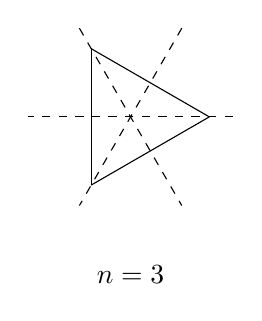
\begin{tikzpicture}[baseline=(0:0cm)]
		\foreach \x in {0,120,240}
			\draw (\x :1cm) -- (\x + 120 :1cm);
		\foreach \x in {0,60,120}
			\draw[dashed] (\x :1.3cm) -- (\x + 180 :1.3cm);
		\node at (270:2cm) {$n=3$};
	\end{tikzpicture} \qquad 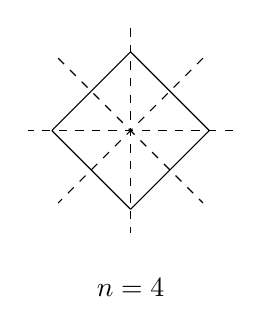
\begin{tikzpicture}[baseline=(0:0cm)]
		\foreach \x in {0,90,...,270}
			\draw (\x :1cm) -- (\x + 90 :1cm);
		\foreach \x in {0,45,...,135}
			\draw[dashed] (\x :1.3cm) -- (\x + 180 :1.3cm);
		\node at (270:2cm) {$n=4$};
	\end{tikzpicture} \qquad 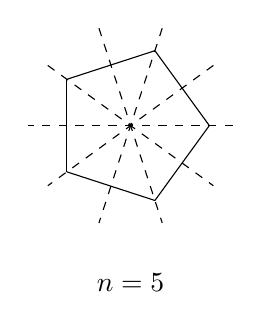
\begin{tikzpicture}[baseline=(0:0cm)]
		\foreach \x in {0,72,...,288}
			\draw (\x :1cm) -- (\x + 72 :1cm);
		\foreach \x in {0,36,...,144}
			\draw[dashed] (\x :1.3cm) -- (\x + 180 :1.3cm);
		\node at (270:2cm) {$n=5$};
	\end{tikzpicture}\end{center}
	Subgrup $N = \Z/n\Z$ bersesuaian dengan rotasi yang mempertahankan segi-$n$ beraturan itu (sudut rotasi $k + n\Z$ adalah $\frac{2\pi k}{n}$), sedangkan $n$ unsur sisanya merupakan pencerminan terhadap garis-garis putus-putus pada gambar. Sebagai contoh, $\tau$ dapat diambil sebagai pencerminan terhadap sumbu horizontal. Silakan pembaca memeriksanya.
\end{example}

Penulisan $G = NH \simeq N \rtimes H$ juga disebut dekomposisi produk semilangsung internal, sebab $NH$ dideskripsikan melalui struktur perkalian di dalam grup $G$ sendiri, sedangkan $N \rtimes H$ dapat dipandang sebagai konstruksi dari luar. Keduanya merupakan dua sudut pandang atas hal yang sama dan tidak perlu dibedakan secara kaku. Untuk produk langsung, kita juga dapat mengarakterisasi kasus dengan banyak variabel.
\begin{lemma}\label{prop:internal-direct}
	Misalkan $G_1, \ldots, G_n$ merupakan subgrup-subgrup dari grup $G$, dan andaikan bahwa
	\begin{compactitem}
		\item untuk setiap $i$, berlaku $G_i \lhd G$,
		\item untuk setiap $i$, berlaku $G_i \cap (G_1 \cdots \widehat{G_i} \cdots G_n) = \{1\}$, dengan $\widehat{\cdots}$ menyatakan bahwa suku tersebut dihilangkan,
	\end{compactitem}
	maka unsur-unsur $G_i$ dan $G_j$ saling komutatif terhadap perkalian ($i \neq j$). Dalam hal ini, $G_1 \cdots G_n$ merupakan subgrup normal dari $G$, dan
	\begin{align*}
		\prod_{i=1}^n G_i & \stackrel{\sim}{\longrightarrow} G_1 \cdots G_n \\
		(g_1, \ldots, g_n) & \longmapsto g_1 \cdots g_n.
	\end{align*}
	 Jika $G = G_1 \cdots G_n$, isomorfisme $\prod_i G_i \rightiso G$ ini disebut dekomposisi \emph{produk langsung internal} dari $G$.
\end{lemma}
\begin{proof}
	Komutativitas perkalian dan kasus $n=2$ sudah tercakup dalam Lemma \ref{prop:internal-semidirect}. Dari sini juga dapat disimpulkan bahwa, untuk setiap subbarisan $1 \leq i_1 < \cdots < i_m \leq n$, produk $G_{i_1} \cdots G_{i_m}$ tetap merupakan subgrup normal dari $G$. Penerapan Lemma \ref{prop:internal-semidirect} secara rekursif pada $n$ memberikan kasus umum.
\end{proof}

\begin{definition}[Barisan eksak] \label{def:exact-seq-group}\index{zhenghelie@barisan eksak (exact sequence)}
	Tinjau suatu barisan homomorfisme grup
	\[ \cdots \xrightarrow{f_0} G_1 \xrightarrow{f_1} G_2 \xrightarrow{f_2} \cdots \xrightarrow{f_i} G_{i+1} \to \cdots, \]
	yang panjangnya dapat berhingga ataupun tak hingga. Jika untuk setiap $i$ berlaku
	\[ \Image(f_i) = \Ker(f_{i+1}), \]
	maka barisan tersebut disebut \emph{eksak}. Kita sering menyingkat $\{1\}$ sebagai $1$, atau menuliskannya sebagai $0$ dalam notasi aditif. Sebagai contoh, untuk sebarang homomorfisme $\varphi: G \to G'$, barisan $G \to G' \to 1$ eksak jika dan hanya jika $\varphi$ surjektif, barisan $1 \to G \to G'$ eksak jika dan hanya jika $\varphi$ injektif, dan kita selalu mempunyai barisan eksak
	\[ 1 \to \Ker(\varphi) \to G \xrightarrow{\varphi} \Image(\varphi)  \to 1 \]
	dengan $\Ker(\varphi) \to G$ sebagai pemetaan inklusi natural.
\end{definition}
Barisan eksak sering digunakan bersama diagram komutatif (lihat \S\ref{sec:cat-and-morphism}). Kegunaannya baru akan tampak sepenuhnya dalam aljabar homologis.

Barisan eksak berbentuk
\[ 1 \to N \to G \xrightarrow{p} H \to 1 \]
disebut \emph{ekstensi grup}. Jika terdapat diagram komutatif homomorfisme grup\index{qunkuozhang@ekstensi grup (group extension)}
\[\begin{tikzcd}
	1 \arrow[r] & N \arrow[r] \arrow[equal, d] & G \arrow[r, "p"] \arrow[d, "\varphi"] & H \arrow[equal, d] \arrow[r] & 1 \\
	1 \arrow[r] & N \arrow[r] & G' \arrow[r, "{p'}"'] & H \arrow[r] & 1
\end{tikzcd}\]
dengan kedua baris merupakan ekstensi grup, maka $\varphi$ disebut suatu ekuivalensi ekstensi grup. Mudah diperiksa bahwa $\varphi$ pasti merupakan isomorfisme. Untuk $H$ dan $N$ yang diberikan, klasifikasi ekstensi grup hingga ekuivalensi merupakan masalah yang sesekali dijumpai dalam aljabar.

Untuk ekstensi grup $1 \to N \to G \xrightarrow{p} H \to 1$, suatu homomorfisme $s: H \to G$ yang memenuhi $p s = \identity_H$ disebut \emph{pemecahan} dari ekstensi tersebut. Dari sini dapat dibangun hubungan antara produk semilangsung dan ekstensi terpecah, sebagai berikut.
\begin{enumerate}
	\item Misalkan $G = N \rtimes_\alpha H$ suatu produk semilangsung. Maka terdapat ekstensi grup terpecah
		\[ \begin{tikzcd}
			1 \arrow[r] & N \arrow[r] & G \arrow[r, "p"] & H \arrow[bend left=30, l, "s"] \arrow[r] & 1
		\end{tikzcd} \]
		dengan $p: G \to H$ homomorfisme proyeksi $(n, h) \mapsto h$, sedangkan $s: H \hookrightarrow G$ homomorfisme inklusi $s(h) = (1,h)$.
	\item Sebaliknya, jika diberikan ekstensi grup di atas beserta pemecahannya $s$, definisikan $\alpha: H \to \Aut(N)$ melalui pembatasan automorfisme adjoin, $\alpha(h) = \Ad(s(h))|_N$. Maka terdapat ekuivalensi ekstensi grup
		\[ \begin{tikzcd}
			1 \arrow[r] & N \arrow[r] \arrow[equal, d] & N \rtimes_\alpha H \arrow[r] \arrow[d, "\varphi"] & H \arrow[equal, d] \arrow[r] & 1 \\
			1 \arrow[r] & N \arrow[r] & G \arrow[r] & H \arrow[r] & 1
		\end{tikzcd} \]
		dengan $\varphi(n, h) := n s(h)$. Silakan pembaca memeriksa bahwa $\varphi$ memang merupakan homomorfisme grup yang injektif.
\end{enumerate}
\section{Aksi Grup dan Prinsip Pencacahan}\label{sec:group-action}
Baik dari sudut penerapan nyata maupun perkembangan historis, suatu grup abstrak sering dideskripsikan melalui aksinya pada sebuah himpunan, sedangkan pengkajian berbagai aksi grup merupakan sarana penting untuk meneliti sifat-sifat grup. Tujuan pertama bagian ini ialah memperjelas konsep-konsep dasar aksi grup.

\begin{definition}[Aksi monoid]\label{def:monoid-action} \index{qunzuoyong@aksi grup (group action)}
	Misalkan $X$ suatu himpunan dan $M$ suatu monoid. Suatu aksi $M$ pada $X$ didefinisikan sebagai pemetaan
	\[ a: M \times X \to X, \]
	yang disebut pemetaan aksi dan harus memenuhi sifat-sifat berikut:
	\begin{compactenum}[(i)]
		\item untuk setiap $g,g' \in M$ dan $x \in X$, berlaku $a(g', a(g, x)) = a(g'g, x)$ (hukum asosiatif),
		\item untuk setiap $x \in X$, berlaku $a(1, x)=x$.
	\end{compactenum}
	Himpunan yang dilengkapi aksi $M$ disebut himpunan-$M$. Aksi yang untuk setiap $m,x$ memenuhi $a(m,x)=x$ disebut \emph{aksi trivial}. Suatu pemetaan di antara himpunan-$M$, yaitu $f: X \to Y$,
	\[ f(a(m, x)) = a(m, f(x)), \quad m \in M, x \in X \]
	disebut pemetaan $M$-\emph{ekuivarian} jika memenuhi persamaan tersebut. Jika pemetaan-pemetaan ekuivarian
	\begin{tikzcd}
		X \arrow[yshift=0.5ex, r, "f"] & Y \arrow[yshift=-0.5ex, l, "g"]
	\end{tikzcd}
	memenuhi $fg = \identity_Y$, $gf = \identity_X$, maka $f, g$ disebut isomorfisme yang saling invers. Dengan demikian, kita dapat mendefinisikan konsep isomorfisme antara himpunan-$M$.
\end{definition}

\begin{remark}
	Singkatnya, untuk $M$ yang diberikan, semua himpunan-$M$ beserta pemetaan ekuivarian membentuk suatu kategori $M\dcate{Set}$. Secara ketat, ukuran himpunan-$M$ $X$ juga harus dibatasi: kita perlu mengandaikan bahwa $M$ dan $X$ termasuk dalam semesta yang sama dan telah dipilih, yaitu $\mathcal{U}$; lihat Definisi \ref{def:U-cat} beserta pembahasan terkait.
\end{remark}

% Dalam bahasa Contoh \ref{eg:symmetric-group}, suatu aksi $M$ pada $X$ ekuivalen dengan pemberian homomorfisme $M \to \Aut(X)$: setiap $m \in M$ dipetakan ke bijeksi $\left[ x \mapsto a(m,x) \right] \in \Aut(X)$.

Menurut kebiasaan, pemetaan aksi yang melekat pada suatu himpunan-$M$ tidak dituliskan, dan $a(m, x)$ ditulis sebagai $m \cdot x$ atau $mx$. Syarat bagi pemetaan aksi dan ekuivariansinya lalu mengambil bentuk alami
\begin{gather*}
	m'(mx) = (m'm)x, \\
	1 \cdot x = x, \\
	f(mx) = mf(x),
\end{gather*}
dengan $ m, m' \in M, x \in X$. Aksi yang didefinisikan demikian disebut aksi kiri $M$, sebab dinyatakan melalui perkalian kiri oleh $M$. Dengan cara yang sama, kita dapat mendefinisikan aksi kanan $M$, yakni $(x, m) \mapsto xm$. Definisi di atas dapat ditulis ulang butir demi butir, misalnya $(xm)m' = x(mm')$, dan seterusnya. Cara yang sekaligus menangani semuanya ialah menggunakan dualitas: aksi kanan $M$ tidak lain merupakan aksi kiri $M^\text{op}$. Setiap pernyataan dalam bagian ini mengenai aksi kiri memiliki versi kanan yang bersesuaian dan tidak akan diulangi.

\begin{example}
	Untuk setiap himpunan $X$, grup simetris $\mathfrak{S}_X$ beraksi secara alami pada $X$: $a: (\sigma, x) \mapsto \sigma(x)$. Demikian pula, monoid matriks real $n \times n$, yaitu $M_n(\R)$, beraksi pada $\R^n$: dengan memandang unsur $\R^n$ sebagai matriks kolom berukuran $n \times 1$, aksi $(A, x) \mapsto A x$ tidak lain adalah perkalian matriks.
\end{example}

\begin{example}
	Jika grup $G$ beraksi dari kiri pada $X$ dan $Y$ merupakan sebarang himpunan, maka terdapat aksi kiri alami $G$ pada $\{f: \text{pemetaan}\; X \to Y \}$ yang diberikan oleh $a(g,f) = \left[ x \mapsto f(g^{-1}x) \right]$; jika $G$ beraksi dari kanan pada $X$, aksi kiri yang bersesuaian diberikan oleh $[x \mapsto f(xg)]$. Verifikasilah rinciannya.
\end{example}

\begin{example}
	Pembahasan berikut dapat dibandingkan dengan \cite[Contoh 7.2.4]{Zh2}. Misalkan $n \geq 1$, dan misalkan ruang $C_\infty(\R^n)$ merupakan penutupan ruang fungsi turun cepat $\mathscr{S}(\R^n)$ (lihat \cite[Contoh 3.2.7]{Zh1}) di dalam $L^\infty(\R^n)$. Definisikan aksi monoid $(\R_{\geq 0}, +)$ pada $C_\infty(\R^n)$ sebagai berikut:
	\[ a(t, u) =
		\begin{cases}
			G_t \ast u, & t > 0, \\
			u, & t=0,
		\end{cases}\]
	dengan $\ast$ menyatakan konvolusi dan $G_t$ merupakan fungsi kernel panas yang dikenal pada $\R^n$,
	\[ G_t(x) := (4\pi t)^{-\frac{n}{2}} e^{-\|x\|^2 /4t}, \quad x \in \R^n. \]
	Menurut teori persamaan panas, $v(t, \cdot) := a(t, u)$ memenuhi masalah nilai awal $\frac{\partial v}{\partial t} = \Delta v$, $v(0, \cdot) = u(\cdot)$; karena itu, $a$ memang memberikan suatu aksi monoid. Dalam analisis fungsional, aksi ini disebut semigrup operator. Karena hantaran panas menghaluskan singularitas fungsi, aksi ini tidak dapat diperluas menjadi aksi grup $(\R, +)$.
\end{example}

\begin{definition}\index{guidao@orbit (orbit)}\index{wendinghuazi@stabilisator (stabilizer)}\index[sym1]{Stab@$\Stab$}
	Misalkan monoid $M$ beraksi pada $X$. Definisikan
	\begin{compactitem}
		\item himpunan \emph{titik tetap} $X^M := \{x \in X: \forall m \in M, \; mx=x \}$;
		\item untuk $x \in X$, \emph{orbit} $Mx := \{mx : m \in M \}$, yang setiap unsurnya disebut wakil orbit tersebut; orbit $Mx$ merupakan subhimpunan dari $X$ yang stabil di bawah $M$;
		\item dengan notasi di atas, \emph{stabilisatornya} didefinisikan sebagai submonoid dari $M$, yaitu $\Stab_M(x) := \{m \in M : mx=x\}$.
	\end{compactitem}
\end{definition}

Aksi yang paling sering digunakan tetaplah aksi grup. Bagi suatu grup $G$, blok pembangun dasar bagi aksi adalah ruang koset berbentuk $G/H$, dengan pemetaan aksi $(g, xH) \mapsto gxH$. Hasil berikut menjelaskan cara menguraikan himpunan-$G$ umum sebagai gabungan saling lepas ruang-ruang koset. Inilah pula titik awal prinsip pencacahan.

\begin{lemma}\label{prop:orbit-decomp}
	Misalkan grup $G$ beraksi pada $X$. Maka:
	\begin{compactenum}[(i)]
		\item terdapat dekomposisi orbit $X = \bigsqcup_x Gx$, dengan memilih satu wakil $x$ dari setiap orbit;
		\item untuk setiap $x \in X$, pemetaan
			\begin{align*}
				G/\Stab_G(x) & \longrightarrow Gx \\
				g \cdot \Stab_G(x) & \longmapsto gx
			\end{align*}
			merupakan isomorfisme antara himpunan-$G$;
		\item khususnya, kita mempunyai persamaan kardinal (lihat \eqref{eqn:cardinal-infinite-sum})
			\[ |X| = \sum_x \left( G: \Stab_G(x) \right); \]
		\item untuk setiap $x \in X$ dan $g \in G$, berlaku
			\[ \Stab_G(gx) = g \Stab_G(x) g^{-1}. \]
	\end{compactenum}
\end{lemma}
\begin{proof}
	Pertama, kita buktikan bahwa jika dua orbit $Gx, Gy$ beririsan, maka $Gx=Gy$. Memang, jika $gx=g'y$, maka $x = g^{-1}g' y \in Gy$, sehingga $Gx \subset Gy$; berdasarkan simetri, diperoleh $Gx=Gy$. Karena $\forall x, \; x = 1\cdot x \in Gx$, dekomposisi orbit segera diperoleh. Pernyataan mengenai pemetaan $G/\Stab_G(x) \to Gx$ merupakan akibat langsung dari definisi stabilisator. Bersama dekomposisi orbit, hal ini menghasilkan persamaan kardinal. Persamaan terakhir dapat diverifikasi langsung dari definisi.
\end{proof}

Dengan demikian, sifat ``$x,y$ berada dalam orbit yang sama'' memberikan suatu relasi ekuivalensi pada $X$. Himpunan hasil bagi yang bersesuaian, atau ruang orbit, dinotasikan dengan $G \backslash X$; bagi aksi kanan, ruang orbit secara alami dinotasikan dengan $X/G$. Perhatikan bahwa memberikan aksi $G$ pada $X$ ekuivalen dengan memberikan homomorfisme $G \to \mathfrak{S}_X$ yang memetakan $g$ ke $[x \mapsto gx]$.
\begin{definition}
	Misalkan $G$ suatu grup dan $X$ suatu himpunan-$G$. Aksi $G$ pada $X$ disebut \index{qunzuoyong!setia (faithful)}\index{qunzuoyong!transitif (transitive)}
	\begin{compactitem}
		\item setia, jika homomorfisme $G \to \mathfrak{S}_X$ yang bersesuaian merupakan injeksi; ini ekuivalen dengan $\bigcap_{x \in X} \Stab_G(x) = \{1\}$;
		\item bebas atau semireguler, jika untuk setiap $x \in X$ berlaku $\Stab_G(x) = \{1\}$;
		\item transitif, jika $X$ hanya mempunyai satu orbit; ini ekuivalen dengan mensyaratkan bahwa $X$ tidak kosong dan, untuk setiap $x, y \in X$, terdapat $g \in G$ sedemikian sehingga $gx=y$;
		\item lebih umum, jika untuk setiap $1 \leq m \leq n$, grup $G$ beraksi secara transitif pada $\{ (x_1, \ldots, x_m) \in X^m: \text{unsur-unsur berbeda} \}$, maka aksi $G$ pada $X$ disebut $n$-transitif.
	\end{compactitem}

	Himpunan-$G$ yang transitif juga disebut \emph{ruang homogen}-$G$, sedangkan ruang homogen-$G$ yang bebas disebut \emph{ruang homogen utama}-$G$ atau \emph{torsor}.\index{qixingkongjian@ruang homogen (homogeneous space)}\index{naozi@torsor (torsor)}
\end{definition}
Sebagai akibat dari Lema \ref{prop:orbit-decomp}, hingga isomorfisme, ruang koset $G/H$ mencakup semua ruang homogen.

Istilah-istilah ini jelas berasal dari geometri, yang untuk itu struktur manifold dan ruang dasar perlu diperkenalkan. Namun, bagian ini hanya membahas himpunan, dan penerapan utamanya adalah masalah pencacahan himpunan; lihat \S\ref{sec:Sylow}. Untuk sementara, mari kita tinjau beberapa contoh umum.

\begin{example}[Aksi translasi dan koset]
	Misalkan $G$ suatu grup dan $H$ subgrupnya. Aksi kiri $H$ pada $G$ yang diberikan oleh $(h, g) \mapsto hg$ disebut aksi translasi kiri. Jelas bahwa
	\begin{inparaenum}[(i)]
		\item orbit-orbit yang bersesuaian tidak lain adalah koset $Hg$ ($g \in G$),
		\item ruang orbitnya tidak lain adalah ruang koset $H \backslash G$,
		\item aksi ini bebas, dan transitif jika dan hanya jika $H=G$.
	\end{inparaenum}
	Pernyataan yang sama berlaku bagi aksi translasi kanan $H$ pada $G$, yaitu $(g,h) \mapsto gh$; ruang orbit yang bersesuaian tidak lain adalah $G/H$.

	Sekarang misalkan $H, K$ subgrup-subgrup dari $G$. Koset ganda mempunyai penafsiran serupa: tinjau aksi kiri $H \times K^\text{op}$ pada $G$,
	\[ ((h, k), g) \mapsto hgk, \quad (h, k) \in H \times K^\text{op}, \; g \in G. \]
	Orbit yang bersesuaian tepat merupakan koset-koset ganda $HgK$ ($g \in G$), sedangkan ruang orbitnya diidentifikasi dengan $H \backslash G/K$. Namun, sifat-sifat lain aksi ini jauh lebih rumit daripada dalam kasus koset kiri atau koset kanan.
\end{example}

\begin{example}[Aksi konjugasi]\label{eg:conj-action} \index{gonge@konjugasi (conjugation)}
	Tetap misalkan $G$ suatu grup. Homomorfisme adjoin $\Ad: G \to \Aut(G)$ memberikan aksi $G$ yang disebut \emph{aksi konjugasi} pada dirinya sendiri, yakni $G \times G \to G$ (di sini kita meninjau aksi kiri). Setelah definisinya diuraikan, aksi ini tidak lain adalah
	\[ (g, x) \longmapsto {}^g x := gxg^{-1}. \]
	Orbit di bawah aksi konjugasi disebut \emph{kelas konjugasi} dalam $G$.

	Lebih umum, untuk sebarang subhimpunan $E \subset G$, kita telah mendefinisikan subgrup $N_G(E)$; aksinya pada $E$ juga disebut konjugasi. Jika dua subhimpunan $E, E'$ memenuhi $\exists g \in G, \; E' = gEg^{-1}$, maka $E$ dan $E'$ disebut saling konjugat.

	Perilaku aksi konjugasi pada grup nonkomutatif umumnya cukup rumit. Untuk $x \in G$, subgrup stabilisatornya tepat merupakan sentralisator $Z_G(x)$, sedangkan himpunan titik tetapnya adalah pusat $Z_G$. Menganalisis aksi konjugasi $G$ merupakan langkah yang tak terelakkan untuk memahami struktur grup tersebut.
\end{example}

Torsor merupakan jenis himpunan-$G$ yang sangat umum dijumpai. Bahasa ini baru menunjukkan kekuatannya apabila dilengkapi latar belakang geometri yang sesuai; lihat \S\ref{sec:group-in-cat}. Berikut hanya diperkenalkan contoh yang paling dasar.
\begin{example}
	Misalkan $G_1$, $G_2$ grup, dan tetapkan
	\[ \Isom(G_1, G_2) := \{ \text{ isomorfisme } \; \varphi: G_1 \to G_2 \}. \]
	Jika $\Isom(G_1, G_2)$ tidak kosong, terdapat aksi kiri $\Aut(G_2)$ padanya, yakni $(g, \varphi) \mapsto g \circ \varphi$, dengan $g \in \Aut(G_2)$. Aksi ini menjadikan $\Isom(G_1, G_2)$ suatu torsor-$\Aut(G_2)$. Walaupun yang ditinjau di sini hanya isomorfisme grup, konstruksi serupa sebenarnya dapat dilakukan dalam sebarang kategori; lihat \S\ref{sec:cat-and-morphism}.

	Kita tentu tidak perlu membatasi diri pada aksi kiri: $\Aut(G_1)$ juga beraksi dari kanan pada $\Isom(G_1, G_2)$ melalui komposisi pemetaan. Aksi di kedua sisi ini memenuhi $(g \circ \varphi) \circ g' = g \circ (\varphi \circ g')$, sehingga dapat digabungkan menjadi aksi $\Aut(G_1)^{\text{op}} \times \Aut(G_2)$. Baik dilihat dari kiri maupun kanan, $\Isom(G_1, G_2)$ merupakan torsor. Struktur semacam ini disebut bitorsor.
\end{example}

Definisi asli torsor agak tidak langsung. Namun, terdapat karakterisasi ringkas berikut, yang akan sangat berguna dalam kerangka teori kategori; lihat \S\ref{sec:group-in-cat}.

\begin{lemma}\label{prop:torsor-criterion}
	Misalkan $X$ suatu himpunan-$G$ yang tidak kosong. Maka $X$ merupakan torsor jika dan hanya jika pemetaan
	\begin{align*}
		\Phi: G \times X & \longrightarrow X \times X \\
		(g, x) &  \longmapsto (x, gx)
	\end{align*}
	merupakan bijeksi.
\end{lemma}
\begin{proof}
	Menurut definisi, $\Phi^{-1}(x,y) = \{g \in G: gx=y\} \times \{x\}$. Karena itu, pemetaan $\Phi$ injektif jika dan hanya jika $X$ bebas, dan surjektif jika dan hanya jika $X$ transitif.
\end{proof}
\section{Sylow 定理}\label{sec:Sylow}
首先引入 $p$-群的概念.

\begin{definition}\label{def:p-group}\index{$p$-群}
	设 $p$ 为素数. 满足 $|G|=p^m$, $m \in \Z_{\geq 0}$ 的群 $G$ 称为 $p$-群.
\end{definition}
应用命题 \ref{prop:Lagrange}, 易见 $p$-群的子群和商群仍是 $p$-群.

\begin{proposition}\label{prop:counting-localization}
	设 $G$ 为非平凡 $p$-群, 则任意有限 $G$-集 $X$ 皆满足
	\[ |X| \equiv \left\lvert X^G \right\rvert \mod p. \]
\end{proposition}
\begin{proof}
	对任意 $x \in X$, 命题 \ref{prop:Lagrange} 蕴涵 $(G: \Stab_G(x))$ 是 $p$ 的幂. 故有
	\[ [ x \notin X^G] \iff [ \Stab_G(x) \neq G ] \iff (G: \Stab_G(x)) \equiv 0 \bmod p . \]
	套入引理 \ref{prop:orbit-decomp} 即得所求.
\end{proof}

\begin{corollary}\label{prop:p-group-center}
	设 $G$ 为非平凡的 $p$-群, 则 $Z_G \neq \{1\}$.
\end{corollary}
\begin{proof}
	考虑 $G$ 的共轭作用 (例 \ref{eg:conj-action}). 由命题 \ref{prop:counting-localization} 得到
	\[ 0 \equiv |G| \equiv |Z_G| \mod p , \]
	故 $|Z_G| > 1$.
\end{proof}

此式可用以递归地研究 $p$-群的结构, 兹举一例.
\begin{corollary}
	设 $G$ 为 $p$-群而 $H \subsetneq G$ 为真子群, 则 $H \subsetneq N_G(H)$. 特别地, $(G:H)=p$ 蕴涵 $H \lhd G$.
\end{corollary}
\begin{proof}
	已知 $Z_G$ 非平凡, 显然 $Z_G \subset N_G(H)$. 若 $Z_G \not\subset H$, 则 $H \subsetneq Z_G H \subset N_G(H)$. 因此不妨假设 $Z_G \subset H$. 现在对 $|G|$ 递归论证: 定义 $\bar{G} := G/Z_G$, $\bar{H} := H/Z_G$, 可假设
	\[ \bar{H} \subsetneq N_{\bar{G}}(\bar{H}). \]
	容易看出 $N_G(H)/Z_G = N_{\bar{G}}(\bar{H})$. 应用命题 \ref{prop:2nd-homomorphism} 即得 $H \subsetneq N_G(H)$.
\end{proof}

另一个直接而重要的推论如下. 先回忆我们在 \S\ref{sec:group-and-monoid} 定义的元素 $x \in G$ 的阶 $\text{ord}(x)$.
\begin{corollary}[Cauchy 定理]\label{prop:group-Cauchy}
	设 $G$ 为有限群, 素数 $p$ 整除 $|G|$, 则存在 $x \in G$ 使得 $\ord(x)=p$.
\end{corollary}
\begin{proof}
	定义集合
	\[ X_p := \{(g_i)_{1 \leq i \leq p} \in G^p : g_1 \cdots g_p = 1 \}. \]
	不妨将下标 $1 \leq i \leq p$ 看成 $\Z/p\Z$ 里的元素. 如此一来循环群 $\Z/p\Z$ 就作用在 $X_p$ 上: 陪集 $m + p\Z$ 的作用是平移下标
	\[ (g_i)_{i \in \Z/p\Z} \longmapsto (g_{i+m})_{i \in \Z/p\Z}. \]
	须证明此作用不逸出 $X_p$, 仅须检查 $m=1$ 的情形: 对等式 $g_1 \cdots g_p = 1$ 左乘以 $g_1^{-1}$, 右乘以 $g_1$ 即是. 由此导出 $(X_p)^{\Z/p\Z} = \{(x, \ldots, x) : x^p = 1 \}$. 注意到 $x^p=1$ 且 $x \neq 1$ 等价于 $\ord(x)=p$ (参看例 \ref{eg:cyclic-group}).

	由于 $g_p = (g_1 \cdots g_{p-1})^{-1}$, 投影映射 $X_p \to G^{p-1}$, $(g_i)_{1 \leq i \leq p} \mapsto (g_i)_{1 \leq i < p}$ 是双射, 故
	\[ |X_p| = |G|^{p-1} \equiv 0 \mod p. \]
	另一方面, 命题 \ref{prop:counting-localization} 给出
	\[ |X_p| \equiv \left\lvert(X_p)^{\Z/p\Z}\right\rvert = 1 + \left\lvert \{x \in G : \ord(x)=p \} \right\rvert \mod p , \]
	故 $\{x \in G : \ord(x)=p \}$ 非空.
\end{proof}

\begin{convention}
	设 $p$ 为素数, $n \in \Z_{\geq 1}$, 若 $p^a \mid n$ 而且 $p^{a+1} \nmid n$, 则写作 $p^a \| n$.
\end{convention}

\begin{definition}\index{Sylow $p$-子群}
	设 $G$ 为 $n$ 阶有限群, $p$ 为素数. 设 $p^m \| n$, 满足 $|H| = p^m$ 的子群 $H$ 称为 $G$ 的 Sylow $p$-子群.
\end{definition}
这意谓 $p$-子群 $H$ 在 Lagrange 定理的约束下达到最大可能阶数. 此定义显然仅在 $p \mid n$ 时才有实质意涵.

\begin{lemma}\label{prop:Wielandt-lemma}
	设 $p$ 为素数. 对任意非负整数 $b \leq a$, $a \neq 0$ 和 $m$, 二项式系数满足同余式
	\[ \binom{p^m a}{p^m b} \equiv \binom{a}{b} \mod p. \]
\end{lemma}
\begin{proof}
	考虑以符号 $T$ 为变元的整系数多项式. 由于 $0 < c < p \implies p \mid \binom{p}{c}$, 故
	\[ (T+1)^{pa} = \left( T^p + p(\cdots) + 1 \right)^a \equiv (T^p + 1)^a \mod p. \]
	即: 两边逐系数模 $p$ 同余. 两侧以二项式定理展开, 比较 $T^{pb}$ 的系数即得 $m=1$ 的情形. 迭代 $m$ 次遂得一般情形.
\end{proof}

\begin{theorem}[Sylow 第一定理]
	对任意素数 $p$, 任意有限群 $G$ 含有 Sylow $p$-子群.
\end{theorem}
下面论证供鉴赏之用, 另有它证如 \cite[Theorem 6.2]{Lang02}.
\begin{proof}[H.\ Wielandt]
	置 $n := |G|$, 不妨假设 $p^m \| n$, $m \geq 1$. 定义
	\[ Y := \left\{ \text{ 子集 } \; E \subset G : |E|=p^m \right\}. \]
	由引理 \ref{prop:Wielandt-lemma} 知
	\[ |Y| = \binom{n}{p^m} \equiv \binom{p^{-m} n}{1} = p^{-m} n \not\equiv 0 \mod p . \]

	群 $G$ 以左平移 $(g, E) \mapsto gE$ 作用于 $Y$. 由引理 \ref{prop:orbit-decomp} 和以上同余式知存在 $E \in Y$ 使得 $p \nmid (G: \Stab_G(E))$, 我们断言 $H := \Stab_G(E)$ 是 Sylow $p$-子群. 首先注意到 $p \nmid \frac{|G|}{|H|}$ 故 $p^m$ 整除 $|H|$. 任取 $g \in E$, 由稳定化子的性质知 $Hg  \subset E$; 配合 $|H|=|Hg|$ 遂得到 $|H| \leq  |E| = p^m$, 故 $|H|=p^m$. 明所欲证.
\end{proof}

\begin{lemma}
	设 $p$ 为素数, 而$P$ 是 $G$ 的 Sylow $p$-子群. 若 $G$ 的 $p$-子群 $H$ 满足 $H \subset N_G(P)$, 则 $H \subset P$.
\end{lemma}
\begin{proof}
	对群 $HP$ 应用命题 \ref{prop:3rd-homomorphism} 可得群同构 $HP/P \simeq H/H \cap P$, 故 $HP$ 仍是 $p$-群. 又因为 $P \subset HP \subset G$ 而 $P$ 是 Sylow $p$-子群, 必有 $HP=P$, 而这又等价于 $H \subset P$.
\end{proof}

\begin{theorem}[Sylow 第二定理]
	令 $G$ 为有限群, $p$ 为素数. 则
	\begin{compactenum}[(i)]
		\item 任意 $p$-子群 $H \subset G$ 皆包含于某个 Sylow $p$-子群;
		\item $G$ 的任两个 Sylow $p$-子群 $P, P'$ 皆共轭;
	\end{compactenum}
	特别地, $G$ 中存在正规的 Sylow $p$-子群 当且仅当 $G$ 有唯一的 Sylow $p$-子群.
\end{theorem}
\begin{proof}
	选定 Sylow $p$-子群 $P \subset G$, 并考虑它在 $G$ 的共轭作用下的轨道
	\[ X := \left\{ gPg^{-1} : g \in G \right\} \]
	任意 $Q \in X$ 都是 $G$ 的 Sylow $p$-子群, 而且其稳定化子群是 $N_G(Q)$. 我们有 $G$-集的同构
	\begin{align*}
		G/N_G(P) & \stackrel{\sim}{\longrightarrow} X \\
		g N_G(P) & \longmapsto gPg^{-1}.
	\end{align*}

	由于 $P \subset N_G(P)$, 我们有 $|X| \not\equiv 0 \mod p$. 现假设 $H \subset G$ 为 $p$-子群, 那么 $H$ 也共轭作用于 $X$ 上. 应用命题 \ref{prop:counting-localization} 得 $X^H$ 非空. 取 $Q \in X^H$, 从定义知 $H \subset N_G(Q)$, 上述引理遂保证 $H \subset Q$, 这就证明了第一个断言. 若进一步要求 $H$ 为  Sylow $p$-子群, 则必有 $H = Q$. 由于 $X$ 中元素相互共轭, 第二个断言随之得证.
\end{proof}

\begin{theorem}[Sylow 第三定理]
	承上, $G$ 中 Sylow $p$-子群的个数 $\equiv 1 \mod p$.
\end{theorem}
\begin{proof}
	沿用上个证明的框架, 选定 Sylow $p$-子群 $P$ 并取 $H = P$, 以上业已证明了 $X^P$ 中的元素必为包含 $P$ 的 $p$-子群, 故 $X^P = \{P\}$. 套回命题 \ref{prop:counting-localization} 遂得 $|X| \equiv \left\lvert X^P \right\rvert = 1 \mod p$.
\end{proof}

\begin{proposition}
	 对每个素数 $p$, 有限群 $G$ 的每个 Sylow $p$-子群皆正规的充分必要条件是 $G = \prod_{p \mid\; |G|} H_p$, 其中 $H_p$ 是 $p$-子群.
\end{proposition}
\begin{proof}
	设 $p_1 < \cdots < p_r$ 为素数. 若 $G$ 同构于直积 $\prod_{i=1}^r H_{p_i}$, 其中 $|H_{p_i}| = p_i^{a_i}$ ($a_i \in \Z_{\geq 1}$), 那么 $H_{p_i}$ 自然地嵌入为 $G$ 的正规 Sylow $p_i$-子群, 而 $|G| = \prod_{i=1}^r p_i^{a_i}$.
	
	反过来设 $|G| = p_1^{a_1} \cdots p_r^{a_r}$, 而且对每个 $1 \leq i \leq r$ 皆有正规 Sylow $p_i$-子群 $H_{p_i}$. 它们的阶数两两互素, 运用命题 \ref{prop:Lagrange} 可以在 $G$ 中验证 $H_{p_i} \cap \prod_{j \neq i} H_{p_j} = \{1\}$. 于是引理 \ref{prop:internal-direct} 的条件成立, 得到同构 $\prod_{i=1}^r H_{p_i} \rightiso H_{p_1} \cdots H_{p_r} \subset G$. 比较阶数可知 $H_{p_1} \cdots H_{p_r} = G$.
\end{proof}

\section{群的合成列}\label{sec:composition-series-grp}
将一个群设法拆解为较小的构件是群论的常见手法, 合成列是其中一例.

\begin{definition}[正规列]\label{def:normal-series}\index{zhengguilie@正规列 (normal series)}
	群 $G$ 的递降子群链
	\[ G = G_0 \supset G_1 \supset \cdots \supset G_n = \{1\} \]
	如满足 $\forall 0 \leq i < n,\;  G_{i+1} \lhd G_i$, 则称之为\emph{正规列}, 而群族
	\[ G_i/G_{i+1}, \quad i=0, \ldots, n-1 \]
	称为该列的\emph{子商}. 正规列的\emph{加细}是透过形如 \index{zishang@子商 (subquotient)}
	\[ \left[ \cdots \supset G_i \supset G_{i+1} \supset \cdots \right] \leadsto \left[ \cdots \supset G_i \supset G' \supset G_{i+1} \supset \cdots \right] \]
	的反复插项得到的新列. 插入 $G' = G_i$ 或 $G_{i+1}$ 得到的加细是平凡的; 反之则称为\emph{真加细}.
\end{definition}

下节将考虑一种特殊的正规列, 在此一并定义.
\begin{definition}[中心列]\label{def:central-series}\index{zhongxinlie@中心列 (central series)}
	群 $G$ 的正规列 $G = G_0 \supset G_1 \supset \cdots$ 如对每个 $i$ 都满足
	\begin{gather*}
		G_i \lhd G, \\
		G_i/G_{i+1} \subset Z_{G/G_{i+1}},
	\end{gather*}
	则称为\emph{中心列}.
\end{definition}

\begin{definition}[合成列]\label{def:composition-series}\index{hechenglie@合成列 (composition series)}
	若群 $G$ 的正规列 $G = G_0 \supset G_1 \supset \cdots$ 满足 $G_{i+1} \subsetneq G_i$, 而且子商皆为单群, 则称之为\emph{合成列}.
\end{definition}
细观单群定义可见合成列正是无冗余项, 而且无法再(真)加细的列. 有限群总有合成列, 一般的群则未必.

\begin{lemma}[Zassenhaus 引理]\label{prop:Zassenhaus}
	固定群 $G$, 考虑子群 $U, V$ 及各自的正规子群 $u \lhd U$, $v \lhd V$. 则有
	\begin{gather*}
		u(U \cap v) \lhd u(U \cap V), \\
		(u \cap V) v \lhd (U \cap V)v,
	\end{gather*}
	其中各项在注记 \ref{rem:HN} 的意义下都是子群, 而且有自然的同构
	\[ \dfrac{u (U \cap V)}{u (U \cap v)} \simeq \dfrac{(U \cap V)v}{(u \cap V)v}. \]
\end{lemma}
\begin{proof}
	我们将表解各子群之间的关系, 图例如下:
	\[ \begin{tikzcd}
		G \arrow[dash, d] \\ H: \text{子群}
	\end{tikzcd} \quad
	\begin{tikzcd}
		G \arrow[dash, d, "\triangledown" description] \\ N: \text{正规子群}
	\end{tikzcd} \quad
	\begin{tikzcd}[column sep=tiny]
		A \arrow[dash, rd] & & B \arrow[dash, ld] \\
		& A \cap B &
	\end{tikzcd} \quad
	\begin{tikzcd}[column sep=tiny]
		{}& HN \arrow[dash, ld] \arrow[dash, rd, "\triangledown" description] & \\
		H & & N
	\end{tikzcd}\]
	其中 $H \subset N_G(N)$. 现断言有以下图表:
	\[ \begin{tikzcd}[column sep=tiny]
		{} & U \arrow[dash, d] & & V \arrow[dash, d] & \\
		& u(U \cap V) \arrow[dash, dd, "\triangledown" description] \arrow[dash, rd] & & (U \cap V)v \arrow[dash, dd, "\triangledown" description] \arrow[dash, ld] & \\
		& & U \cap V \arrow[dash, dd, "\triangledown" description] & & \\
		& u(U \cap v) \arrow[dash, ld] \arrow[dash, rd] & & (u \cap V)v \arrow[dash, ld] \arrow[dash, rd] & \\
		u \arrow[dash, rd] & & (u \cap V)(U \cap v) \arrow[dash, ld] \arrow[dash, rd] & & v \arrow[dash, ld] \\
		& u \cap V & & U \cap v &
	\end{tikzcd} \]
	首先留意有性质 $U \cap V \subset N_G(u) \cap N_G(v)$ 等等, 图中的积 $u(U \cap V)$ 等因而是子群. 图例第一条 (即: 子群在下) 显然成立. 又可逐一验证
	\begin{align*}
		u(U \cap v) \cap (U \cap V) & = (u \cap V)(U \cap v) = (U \cap V) \cap (u \cap V)v, \\
		u \cap (u \cap V)(U \cap v) & = u \cap V, \\
		(u \cap V)(U \cap v) \cap v & = U \cap v.
	\end{align*}
	故图例第三条 (子群交) 也成立. 同理可验证图例第四条 (子群积). 至于第二条 (正规子群), 从 $v \lhd V$ 可导出 $U \cap v \lhd U \cap V$, 从而 $u(U \cap v) \lhd u(U \cap V)$; 同理有 $(u \cap V)v \lhd (U \cap V)v$, 取交即得 $(u \cap V)(U \cap v) \lhd U \cap V$. 至此证成断言.

	现在考虑图表中的两个平行四边形. 分别运用命题 \ref{prop:3rd-homomorphism} 可得自然同构
	\begin{equation*}\begin{tikzcd}[column sep=tiny, row sep=small]
		\dfrac{u (U \cap V)}{u(U \cap v)} \arrow[rd, "\simeq"'] &  & \dfrac{(U \cap V)v}{(u \cap V)v} \arrow[ld, "\simeq"] \\
		& \dfrac{U \cap V}{(u \cap V)(U \cap v)} &
	\end{tikzcd}\end{equation*}
	明所欲证.
\end{proof}

\begin{definition}\label{def:JH-subquotients}
	设 $G = G_0 \supset \cdots$ 为正规列, 我们视其子商 $(G_i/G_{i+1})_{i \geq 0}$ 为不计顺序, 但计入重数的集合. 如果两个正规列长度相同, 而且其子商在上述意义下相等, 则称两正规列\emph{等价}.
\end{definition}

\begin{theorem}[Schreier 加细定理]\label{prop:Schreier}
	设
	\begin{align*}
		G & = G_0 \supset \cdots \supset G_r \supset G_{r+1} = \{1\}, \\
		G & = H_0 \supset \cdots \supset H_s \supset H_{s+1} = \{1\}
	\end{align*}
	为 $G$ 的两个正规列, 则两者有等价的加细.
\end{theorem}
\begin{proof}
	对每个 $0 \leq i \leq r$, $0 \leq j \leq s$ 定义
	\begin{align*}
		G_{i,j} & := G_{i+1} (H_j \cap G_i), \\
		H_{j,i} & := (G_i \cap H_j) H_{j+1}.
	\end{align*}
	先看 $G_{i,j}$, 由 $G_{i+1} \lhd G_i$ 知其为子群. 包含关系 $G_{i, j+1} \lhd G_{i,j}$ 成立, 而且
	\[ G_{i,0} = G_{i+1} (G \cap G_i) = G_i, \quad G_{i,s+1} = G_{i+1}, \]
	遂得到 $(G_i)_{i=0}^r$ 的加细
	\[ \mathcal{G} := \left[ \cdots \supset G_i = G_{i, 0} \supset G_{i, 1} \supset \cdots G_{i, s} \supset G_{i, s+1}= G_{i+1} \supset \cdots \right] . \]
	同理可见 $H_{j, i}$ 给出 $(H_j)_{j=0}^s$ 的加细, 记为 $\mathcal{H}$. 在引理 \ref{prop:Zassenhaus} 中取 $u := G_{i+1}$, $U := G_i$ 和 $v := H_{j+1}$, $V := H_j$, 遂导出
	\[ \dfrac{G_{i,j}}{G_{i,j+1}} = \dfrac{u(U \cap V)}{u(U \cap v)} \simeq \dfrac{(U \cap V)v}{(u \cap V)v} = \dfrac{H_{j,i}}{H_{j,i+1}}. \]

	当 $(i,j)$ 取遍所有可能, 正规列 $\mathcal{G}$, $\mathcal{H}$ 的各个子商在同构两边都恰好出现一次. 证毕.
\end{proof}

\begin{theorem}[Jordan--Hölder 定理]\label{prop:JH-group}\index{Jordan--Hölder 定理}
	群 $G$ 的任两个合成列皆等价.
\end{theorem}
\begin{proof}
	这是定理 \ref{prop:Schreier} 配合定义 \ref{def:composition-series} 的直接推论.
\end{proof}

因此, 一旦群 $G$ 有合成列, 则其子商在定义 \ref{def:JH-subquotients} 的意义下无关合成列的选取.
\begin{definition}\index{hechengyinzi@合成因子 (composition factor)}
	假设群 $G$ 有合成列, 定义其\emph{合成因子}或 Jordan--Hölder 因子集 $\text{JH}(G)$ 为其任意合成列的全体子商 (不计顺序, 计入重数).
\end{definition}

带重数集 $\text{JH}(G)$ 是一种管用的不变量, 但它无法在同构意义下刻画群. 例如群 $\Z/4\Z$ 与 $\Z/2\Z \times \Z/2\Z$ 的合成因子都是 $\{ \Z/2\Z, \Z/2\Z\}$, 但两群不同构.

此外, 给定群的正合列 $1 \to N \to G \xrightarrow{\pi} Q \to 1$. 假设 $N$, $Q$ 皆有合成列, 则 $G$ 亦有合成列, 而且
\begin{gather}\label{eqn:JH-ses}
	\text{JH}(G) = \text{JH}(N) \cup  \text{JH}(Q),
\end{gather}
这里的并集当然是计入重数的. 论证如下: 分别考虑 $Q$ 和 $N$ 的合成列 $(Q_i)_i$, $(N_j)_j$, 两者可以衔接成合成列
\[ G \supset \pi^{-1}(Q_1) \supset \cdots \supset \pi^{-1}(Q_r) = N \supset N_1 \supset \cdots . \]
其合成因子正是 $\text{JH}(N) \cup  \text{JH}(Q)$.

\begin{proposition}\label{prop:abelian-composition-series}
	若 $G$ 为有限交换群, 则 $\text{JH}(G)$ 中的元素都是素数阶群.
\end{proposition}
留意: 素数阶群都是循环群.
\begin{proof}
	可假设 $G$ 非平凡群. 推论 \ref{prop:group-Cauchy} 确保存在素数 $p$ 及 $p$ 阶元素 $t \in G$. 考虑交换群的正合列
	\[ 1 \to \lrangle{t} \to G \to G/\lrangle{t} \to 1 \]
	并利用 \eqref{eqn:JH-ses} 施递归于 $|G|$, 即得所求.
\end{proof}

我们将在推论 \ref{prop:finite-abelian-structure} 详细描述有限交换群的结构.

\section{可解群与幂零群}\label{sec:solvable-groups}
可解群的概念源于 Galois 对高次方程根式解的研究, 幂零与超可解群则是其变体. 这些概念在 Lie 群, Lie 代数的研究中占有重要地位, 本节主要介绍其群论的面向. 请先回忆定义 \ref{def:normal-series}, \ref{def:central-series} 中的子群列.

\begin{definition}\label{def:solvable-nilpotent-group}\index{kejiequn@可解群 (solvable group)}\index{chaokejiequn@超可解群 (supersolvable group)}\index{milingqun@幂零群 (nilpotent group)}
	设 $G$ 为群.
	\begin{enumerate}
		\item 若存在正规列 $G = G_0 \supset G_1 \supset \cdots \supset G_r = \{1\}$ 使得每个子商都交换, 则称之为\emph{可解群};
		\item 承上, 若对每个 $i$ 皆有 $G_i \lhd G$, 且 $G_i/G_{i+1}$ 是素数阶循环群, 则称之为\emph{超可解群};
		\item 如果存在中心列 $G = G_0 \supset G_1 \supset \cdots \supset G_r = \{1\}$, 则称之为\emph{幂零群}.
	\end{enumerate}
\end{definition}

我们希望在上述定义中找到一类典则的正规列/中心列, 借以检验一个群是否可解或幂零. 以下概念是必要的.
\begin{definition}\index[sym1]{$[x,y]$}
	对于 $x, y \in G$, 定义\emph{换位子}
	\[ [x,y] := xyx^{-1}y^{-1}. \]
	对任意子集 $A, B \subset G$, 置 $[A, B] \lhd G$ 为包含 $\{[a,b] : a \in A, b \in B\}$ 的最小正规子群, 或简称为它们生成的正规子群. 递归地定义 $G$ 之
	\begin{itemize}
		\item \emph{导出列}: \begin{tikzpicture}[baseline] \matrix (M) [matrix of math nodes, left delimiter={\{} ] {
			\mathscr{D}^{i+1} G := [\mathscr{D}^i G, \mathscr{D}^i G] \\
			\mathscr{D}^0 G := G, \\
		}; \node at (M-1-1.east) [right=1em] {($i \geq 0$)}; \end{tikzpicture}
		\item \emph{降中心列}: \begin{tikzpicture}[baseline] \matrix (M) [matrix of math nodes, left delimiter={\{} ] {
			\mathscr{C}^{i+1} G := [\mathscr{C}^i G, G] \\
			\mathscr{C}^0 G := G. \\
		}; \node at (M-1-1.east) [right=1em] {($i \geq 0$)}; \end{tikzpicture}
	\end{itemize}
\end{definition}

容易验证以下性质. 设 $i \in \Z_{\geq 0}$:
\begin{compactitem}
	\item $xy=yx \iff [x,y]=1$, 而 $[x,y]^{-1} = [y,x]$;
	\item 对于任意群同态 $\varphi: G_1 \to G_2$, 有 $\varphi [x,y] = [\varphi(x), \varphi(y)]$;
	\item $\mathscr{D}^i G \subset \mathscr{C}^i G$;
	\item $\mathscr{D}^i G \lhd G$, $\mathscr{C}^i G \lhd G$: 事实上 $G$ 的任何自同构都保持子群 $\mathscr{D}^i G$ 和 $\mathscr{C}^i G$.
\end{compactitem}
关于 $\mathscr{D}^i G$, $\mathscr{C}^i G$ 的性质可以递归地证明. 我们也称 $G_\text{der} := \mathscr{D}^1 G$ 为 $G$ 的\emph{导出子群}. 而 $G_\text{ab} := G/G_\text{der}$ 称为 $G$ 的\emph{交换化}. 下述泛性质表明了 $G \twoheadrightarrow G_\text{ab}$ 是 $G$ 的``极大交换商''. \index{daochuziqun@导出子群 (derived subgroup)}\index[sym1]{$G_\text{der}$} \index[sym1]{$G_\text{ab}$}

\begin{lemma}\label{prop:abelianization}
	商群 $G_{\mathrm{ab}}$ 是交换群. 对任意交换群 $A$ 和同态 $\varphi: G \to A$, 存在唯一的同态 $\psi: G_{\mathrm{ab}} \to A$ 使下图交换.
	\[ \begin{tikzcd}
		G \arrow[twoheadrightarrow, r] \arrow[d, "\varphi"'] & G_{\mathrm{ab}} \arrow[dashed, ld, "{\exists ! \; \psi}"] \\
		A &
	\end{tikzcd} \]
	特别地, 商群 $G/N$ 交换当且仅当 $N \supset G_\text{der}$, 相应地有商同态 $G_{\mathrm{ab}} \twoheadrightarrow G/N$.
\end{lemma}
\begin{proof}
	设 $x,y \in G$ 映至 $\bar{x}, \bar{y} \in G/G_\text{der}$, 则 $[\bar{x}, \bar{y}]$ 是 $[x,y] \in G_\text{der}$ 的像, 故平凡. 关于 $\psi$ 的存在性相当于 $\Ker(\varphi) \supset G_\text{der}$, 由 $1 = [\varphi(x), \varphi(y)] = \varphi([x,y])$ 立可导出. 唯一性则缘于  $\psi(\bar{x}) = \varphi(x)$.
\end{proof}

\begin{lemma}\label{prop:solvable-nilpotent-characterization}
	对任意群 $G$,
	\begin{compactenum}[(i)]
		\item 对每个 $i$, 商群 $\mathscr{D}^i G/\mathscr{D}^{i+1} G$ 交换, 而 $\mathscr{C}^i G/\mathscr{C}^{i+1} G$ 包含于 $Z_{G/\mathscr{C}^{i+1} G}$;
		\item 群 $G$ 可解当且仅当 $n$ 充分大时 $\mathscr{D}^n G = \{1\}$;
		\item 群 $G$ 幂零当且仅当 $n$ 充分大时 $\mathscr{C}^n G = \{1\}$.
	\end{compactenum}
\end{lemma}
\begin{proof}
	先证 (i). 商群 $\mathscr{D}^i G/\mathscr{D}^{i+1} G$ 交换缘于引理 \ref{prop:abelianization}. 另一方面, 置 $\bar{G} := G/\mathscr{C}^{i+1}G$; 据定义 $[\mathscr{C}^i G, G] \subset \mathscr{C}^{i+1}G$ 等价于 $[\mathscr{C}^i G/\mathscr{C}^{i+1} G, \;\bar{G}] = \{1\}$, 后者又等价于 $\mathscr{C}^i G/\mathscr{C}^{i+1} G \subset Z_{\bar{G}}$.

	现证 (ii). 假设有正规列 $G = G_0 \supset G_1 \supset \cdots \supset G_r = \{1\}$, 其子商皆交换. 对 $G \twoheadrightarrow G/G_1$ 应用引理 \ref{prop:abelianization} 可得 $\mathscr{D}^1 G \subset G_1$. 由此递归地对所有 $i \geq 0$ 导出 $\mathscr{D}^i G \subset G_i$. 是以 $\mathscr{D}^r G = \{1\}$. 反之若 $\mathscr{D}^r G = \{1\}$, 则正规列 $G_i := \mathscr{D}^i G$ 满足所需条件.

	对 (iii) 的证明类似. 设有中心列 $G = G_0 \supset G_1 \supset \cdots \supset G_r = \{1\}$. 对 (i) 的论证中业已说明了 $G_i/G_{i+1} \subset Z_{G/G_{i+1}}$ 蕴涵 $[G_i, G] \subset G_{i+1}$ ($i=0$ 的情形是显然的), 故可递归地导出 $\mathscr{C}^i G \subset G_i$, 故 $\mathscr{C}^r G = \{1\}$. 反之假设 $\mathscr{C}^r G = \{1\}$, 那么 $G_i := \mathscr{C}^i G$ 给出所求的中心列. 证毕.
\end{proof}

\begin{remark}
	设 $G$ 为幂零群, $\mathscr{C}^n G = \{1\}$, 则对任意 $x \in G$, 映射 $[x, \cdot]: g \mapsto [x, g]$ 迭代 $n$ 次后的像落在 $\mathscr{C}^n G$, 故成为平凡映射 $g \mapsto 1$. 这解释了``幂零''一词的来由.
\end{remark}

\begin{lemma}\label{prop:solvable-ses}
	设 $G$ 为群, 用 $\mathcal{P}$ 代表可解, 超可解或幂零三种性质之一.
	\begin{compactitem}
		\item 若 $G$ 具有性质 $\mathcal{P}$, 则 $G$ 的子群和商群都有性质 $\mathcal{P}$;
		\item 设 $N \lhd G$, 令 $\bar{G} := G/N$, 则 $G$ 可解当且仅当 $N, \bar{G}$ 皆可解.
	\end{compactitem}
\end{lemma}
\begin{proof}
	设 $N$ 是 $G$ 的子群, $\bar{G}$ 是 $G$ 的商群. 由定义知 $\mathscr{D}^i N \subset \mathscr{D}^i G$, 而 $\mathscr{D}^i \bar{G}$ 是 $\mathscr{D}^i G$ 的商群; 类似性质对 $\mathscr{C}^i G$ 亦成立. 由此知性质 $\mathcal{P} \in \left\{\text{可解}, \text{幂零}\right\}$ 传递到 $N$ 和 $\bar{G}$ 上. 接着证明 $N \lhd G$ 和 $\bar{G} = G/N$ 皆可解蕴涵 $G$ 可解: 假设 $\mathscr{D}^r \bar{G} = \{1\}$ 且 $\mathscr{D}^s N = \{1\}$, 则 $\mathscr{D}^r G \subset N$, 而 $\mathscr{D}^{r+s} G \subset \mathscr{D}^s N = \{1\}$, 故 $G$ 可解.

	最后证明超可解性可以传递到子群 $N$ 和商群 $\bar{G}$. 设有 $G = G_0 \supset \cdots \supset G_r = \{1\}$ 使得 $G_i \lhd G$ 且各子商皆为素数阶循环群. 取 $N_i := N \cap G_i$ 及 $\bar{G}_i := \pi(G_i)$ (正规情形), 其中 $\pi: G \to \bar{G}$ 是满同态, 分别得到 $N$ 与 $\bar{G}$ 中满足类似性质的子群列, 故 $N, \bar{G}$ 皆为超可解群.
\end{proof}

由 $\mathscr{D}^i G \subset \mathscr{C}^i G$ 知幂零蕴涵可解. 事实上还有下述稍强的结果.
\begin{lemma}
	对于有限群, 幂零 $\implies$ 超可解 $\implies$ 可解.
\end{lemma}
\begin{proof}
	显然超可解蕴涵可解. 现给定幂零群 $G$, 假设 $\mathscr{C}^{r+1}G = \{1\}$. 已知 $\mathscr{C}^r G$ 包含于 $G = G/\mathscr{C}^{r+1} G$ 的中心; 特别地, 它是交换群. 故可取其中的合成列
	\[ \mathscr{C}^r G = V_0 \supset V_1 \supset \cdots \supset V_{s+1} = \{1\} \]
	使其子商皆为素数阶循环群 (命题 \ref{prop:abelian-composition-series}). 对降中心列的长度 $r$ 作归纳, 知 $\bar{G} := G/\mathscr{C}^r G$ 也有正规列
	\[ \bar{G} = \bar{G}_0  \supset \cdots \supset \bar{G}_{t+1} = \{1\}, \quad \bar{G}_i \lhd \bar{G} \]
	满足与 $(V_i)_i$ 相同的性质. 取 $G_i$ 为 $\bar{G}_i$ 在 $G$ 中原像, 则 $G_i \lhd G$; 另一方面, $V_j \subset \mathscr{C}^r G \subset Z_G$ 蕴涵 $V_j \lhd G$. 于是子群列
	\[ G = G_0 \supset \cdots \supset G_t \supset V_0 \supset \cdots \supset V_{s+1} = \{1\} \]
	满足超可解群所需条件.
\end{proof}

关于可解有限群最著名的结果当属 Feit--Thompson 定理 \cite{FT63}: 任意奇数阶有限群皆可解. 该定理曾经有力地推动了有限群的分类工作; 作为一篇有限群论的论文, 其长度与繁复亦属空前, 然而还远远不是绝后的.\index{Feit--Thompson 定理}

\begin{example}
	可解群的典型例子是上三角矩阵群. 具体地说, 选定任意域 $\Bbbk$, 记 $\GL(n,\Bbbk)$ 为 $\Bbbk$ 上的 $n \times n$ 可逆矩阵对乘法构成的群 ($n \in \Z_{\geq 1}$). 考虑 $\GL(n, \Bbbk)$ 的如下子群
	\[
		B := \begin{pmatrix}
		* & \cdots & & * \\
		& \ddots & & \vdots \\
		0 & & & *
	\end{pmatrix} \; \supset \;
		U := \begin{pmatrix}
		1 & \cdots & & * \\
		& \ddots & & \vdots \\
		0 & & & 1
	\end{pmatrix} \]
	其中 $*$ 表任意元素, 此外对 $B$, $U$ 分别要求对角元全可逆和全为 $1$. 那么 $B$ 是可解群, $U$ 是幂零群. 这些性质可以用矩阵计算说明, 但这里从抽象观点考察或许更合适: 以下设 $\mathcal{V}$ 为 $n$ 维 $\Bbbk$-向量空间. 考虑线性子空间链
	\[ \mathcal{V} = \mathcal{V}_0 \supset \cdots \supset \mathcal{V}_n = \{0\}, \quad \dim_\Bbbk \mathcal{V}_i/\mathcal{V}_{i+1} = 1 \quad (0 \leq i < n). \]
	方便起见, 对 $m > n$ 置 $\mathcal{V}_m := \{0\}$. 记 $\mathcal{V}$ 的线性自同构群为 $\GL(\mathcal{V})$. 命
	\begin{equation*}
		U_r := \left\{ x \in \GL(\mathcal{V}) : \forall i, \; (x - 1)(\mathcal{V}_i) \subset \mathcal{V}_{i+r} \right\}, \quad r \in \Z_{\geq 1};
	\end{equation*}
	当然, $1$ 代表恒等映射. 显然 $U_1 \supset U_2 \supset \cdots \supset U_n = \{1\}$. 一并留意到 $U_r$ 的定义蕴涵 $\forall i, \; x(\mathcal{V}_i) \subset \mathcal{V}_i$. 我们断言每个 $U_r$ 都是子群, 而且对所有 $r,s$ 都有 $[U_r, U_s] \subset U_{r+s}$.

	首先, 若 $x, x' \in U_r$, 则 $xx' - 1 = (x-1)x' + (x'-1)$ 依然将每个 $\mathcal{V}_i$ 映入 $\mathcal{V}_{i+r}$, 故 $U_r$ 对乘法封闭. 若 $x = 1-X \in U_r$, 则 $\End_\Bbbk(\mathcal{V})$ 中的等式 $X^n=0$ 和
	\[ (1-X)^{-1} = \sum_{k=0}^{n-1} X^k = 1 + X \sum_{k=1}^{n-1} X^{k-1} \; \in U_r, \]
	说明 $U_r$ 对取逆封闭. 现在设 $x = 1-X \in U_r$ 而 $y = 1-Y \in U_s$. 按上式在 $\End_\Bbbk(\mathcal{V})$ 中展开 $[y,x] = y x y^{-1} x^{-1}$. 为了方便集项, 我们用 $qX, vY$ 取代 $X, Y$, 其中 $q,v$ 是形式变元; 这相当于容许线性变换的系数为 $q,v$ 的多项式. 于是
	\begin{multline*}
		(1-vY) (1-qX) (1-vY)^{-1} (1-qX)^{-1} = (1-vY) (1-qX) \cdot \sum_{h=0}^{n-1} v^h Y^h \cdot \sum_{k=0}^{n-1} q^k X^k \\
		= \text{常数项} + \text{仅含 $q$ 的项} + \text{仅含 $v$ 的项} + \text{含 $qv$ 的项}.
	\end{multline*}
	左式代入 $q=v=0$ 可知常数项为 $1$; 代入 $v=0$ (或 $q=0$) 可知仅含 $q$ (或仅含 $v$) 的项为 $0$; 代入 $q=v=1$ 则得到 $[y,x]$: 其中含 $qv$ 的项同时有 $X$ 和 $Y$ 出现, 这样的项必将 $\mathcal{V}_i$ 映入 $\mathcal{V}_{i+r+s}$. 综之 $[x,y]^{-1} = [y,x] \in U_{r+s}$, 于是证出了 $[U_r, U_s] \subset U_{r+s}$. 作为推论, $xyx^{-1} = [x,y]y$ 导致 $r \geq s \implies U_r \lhd U_s$.
	
	以下定义 $U := U_1$. 于是乎 $U_r \lhd U$ 和 $[U_r, U] \subset U_{r+1}$. 这说明 $(U_r)_{1 \leq r \leq n}$ 是 $U$ 的中心列, 从而 $U$ 是幂零群. 我们有满的群同态 $\Phi$
	\begin{align*}
		B := \left\{ x \in \GL(\mathcal{V}): \forall i, \; x (\mathcal{V}_i) \subset \mathcal{V}_i \right\} & \stackrel{\Phi}{\twoheadrightarrow} \bigoplus_{i=0}^{n-1} \GL\left( \mathcal{V}_i/\mathcal{V}_{i+1} \right) \simeq (\Bbbk^\times)^n, \\
		x & \mapsto \left( x \big|_{\mathcal{V}_i/\mathcal{V}_{i+1}} \right)_{i=0}^{n-1} ,
	\end{align*}
	其中因为 $x$ 保持每个 $\mathcal{V}_i$, 可取 $x$ 在每个子商 $\mathcal{V}_i/\mathcal{V}_{i+1}$ 上的诱导自同构. 显然 $\Ker(\Phi) = U$, 所以 $U \lhd B$ 而且 $B/U \simeq \Image(\Phi)$ 交换. 若取定 $\mathcal{V}$ 的基 $e_1, \ldots, e_n$ 使得
	\[ \mathcal{V}_i = \bigoplus_{1 \leq j \leq n-i} \Bbbk e_j \]
	并且将 $\GL(\mathcal{V})$ 中的元素写成矩阵, 一切回归之前对 $B, U$ 的矩阵定义, 而 $x|_{\mathcal{V}_i/\mathcal{V}_{i+1}}$ 恰是 $x$ 的第 $i$ 个对角元. 从 $B/U$ 交换和引理 \ref{prop:solvable-ses} 立见 $B$ 可解.
\end{example}

现在考虑另一种构造. 对于群 $G$, 取 $Z^0 = \{1\}$, 并递归地定义 $Z^{i+1} \lhd G$ 为 $Z_{G/Z^i}$ 对商同态 $G \twoheadrightarrow G/Z^i$ 的原像 ($i \geq 0$). 因此 $Z^{i+1} \supset Z^i$. 称 $\{1\} = Z^0 \subset Z^1 \subset \cdots $ 为群 $G$ 的\emph{升中心列}. 设若存在 $n$ 使得 $Z^n = G$, 逆序观察遂得 $G = Z^n \supset Z^{n-1} \supset \cdots \supset Z^0 = \{1\}$, 由构造易知此为 $G$ 的中心列, 故此时 $G$ 幂零.

\begin{proposition}\label{prop:p-group-nilpotent}
	令 $p$ 为素数, 则有限 $p$-群皆幂零.
\end{proposition}
\begin{proof}
	设 $|G|=p^n$. 考虑 $G$ 的升中心列 $(Z^i)_i$; 由前述观察知对每个 $i \geq 0$, 或者 $Z^i = G$ 或者 $G/Z^i$ 是非平凡 $p$-群. 后一情形下推论 \ref{prop:p-group-center} 蕴涵 $Z_{G/Z^i} \neq \{1\}$ 故 $Z^{i+1} \supsetneq Z^i$, 此时 $p \mid (Z^{i+1} : Z^i)$. 于是升中心列必须在 $n$ 步内止于 $G$.
\end{proof}

\begin{example}\index{Heisenberg 群}
	Heisenberg 群是一类特别的幂零群. 为方便起见, 我们仅在实数域 $\R$ 上操作. 考虑一个有限维 $\R$-向量空间 $W$ 连同其上的非退化双线性型
	\[ \lrangle{\cdot|\cdot}: W \times W \to \R, \]
	并假设 $\lrangle{\cdot|\cdot}$ 反对称: $\forall w, w', \; \lrangle{w|w'} = -\lrangle{w'|w}$; 这类双线性型称作辛形式. 定义
	\[ \mathcal{H}(W) := \R \times W, \]
	其上的二元运算定为
	\[ (t, X) \cdot (s, Y) := \left( t+s+\frac{\lrangle{X,Y}}{2}, X+Y \right). \]
	请读者验证 $\mathcal{H}(W)$ 满足群公理, 而且 $\R = \R \times \{0\}$ 正是 $\mathcal{H}(W)$ 的中心. 我们有群的正合列
	\[ 0 \to \R \to \mathcal{H}(W) \to W \to 0 \]
	其中 $\R$ 和 $W$ 对加法构成群. 因而 $\mathcal{H}(W) \supset \R \supset \{0\}$ 是中心列, $\mathcal{H}(W)$ 是幂零群.

	为说明 Heisenberg 群的来由, 下面取定 $n$ 维 $\R$-向量空间 $V$. 我们须考虑 $V$ 上的某个复值函数空间, 具体选取无关宏旨, 以下不妨就使用速降函数空间 $\mathscr{S}(V) \ni f$; 定义其上的算子空间
	\begin{align*}
		L' & := \left\{ f \mapsto xf : x \in \Hom_\R(V, \R) \right\} \quad (\text{逐点乘以 }\; x), \\
		L & := \left\{ f \mapsto \partial_v f : v \in V \right\} \quad (\text{方向导数}).
	\end{align*}
	若选取 $V$ 的一组基 $v_1, \ldots, v_n$ 及其对偶基 $x_1, \ldots, x_n$ (即: $x_i(v_j) = \delta_{i,j}$), 那么 $\partial_{v_1}, \ldots, \partial_{v_n}$ 和 $x_1, \ldots, x_n$ 分别构成了 $L$ 和 $L'$ 的基. 对于任意线性算子 $X, Y: \mathscr{S}(V) \to \mathscr{S}(V)$, 相应的换位子 $[X, Y]$ 定义成线性算子 $XY - YX$. 则 $[\cdot, \cdot]$ 是反对称双线性型, 而且对任意 $1 \leq i,j \leq n$ 有
	\begin{gather*}
		[x_i, x_j] = 0, \quad [\partial_{v_i}, \partial_{v_j}] = 0, \\
		[\partial_{v_i}, x_j] = \delta_{i,j} := \begin{cases} 1, & i=j, \\ 0, & i \neq j.  \end{cases}
	\end{gather*}
	这些等式不外是初等数学分析. 由以上关系式知 $L \cap L' = \{0\}$, 且 $[\cdot, \cdot]$ 在向量空间的直和 $W := L \oplus L'$ 上非退化. 如此遂从 $V$ 得到 Heisenberg 群 $\mathcal{H}(W)$. 在量子力学中, 取 $V=\R^3$ 并适当选取量纲使得 $\hbar=1$, 则 $L$ 和 $L'$ 分别由空间中的动量 $p_i := \sqrt{-1}\partial_{v_i}$ 和位置算子 $q_i := x_i$ 张成. 关系式 $[\partial_{v_i}, x_j] = \delta_{i,j}$ 化作量子力学里熟知的典则对易关系. 注意到 $p_i$ 正是 $q_i$ 的 Fourier 变换.
\end{example}

\section{自由群}\label{sec:free-group}
设 $X$ 为集合. 概略地说, $X$ 上的自由群 $\mathbf{F}(X)$ 是由从 $X$ 的元素出发, ``形式地''进行乘法与取逆所能得到的表达式组成的群. 这些表达式称为自由群里的\emph{字}, 也称 $X$ 为字母集. 例如当 $X=\{x,y\}$ 时, $\mathbf{F}(X)$ 是由
\[ 1, x, y, x^{-1}, y^{-1}, xy, yx, x^2, yxy, \cdots \]
等无穷多个字组成的集合. ``自由''意谓字的乘法除群论的基本要求如结合律和 $x x^{-1}=1$ 外, 再无其它约束. 自由群可以由泛性质 (参看 \S\ref{sec:cat-universals}) 刻画. 我们也一并考虑自由幺半群.

\begin{definition}[自由幺半群]\label{def:free-monoid}\index{yaobanqun!自由幺半群 (free monoid)}
	考虑形如 $(\mathbf{M}(X), \iota)$ 的资料, 其中$\mathbf{M}(X)$ 是幺半群而 $\iota: X \to \mathbf{M}(X)$ 是集合间的映射. 若对任意幺半群 $M'$ 及映射 $\iota': X \to M'$, 存在唯一的同态 $\varphi: \mathbf{M}(X) \to M'$ 使得下图交换
	\[ \begin{tikzcd}
		X \arrow[r, "\iota"] \arrow[rd, "{\iota'}"'] & \mathbf{M}(X) \arrow[dashed, d, "{\exists! \varphi}"] \\
		& M'
	\end{tikzcd} \]
	则称 $(\mathbf{M}(X), \iota)$ 为 $X$ 上的自由幺半群.
\end{definition}

\begin{definition}[自由群]\label{def:free-group}\index{qun!自由群 (free group)}
	考虑形如 $(\mathbf{F}(X), \iota)$ 的资料, $\mathbf{F}(X)$ 是群而 $\iota: X \to \mathbf{F}(X)$ 是集合间的映射. 若对任意群 $G$ 及映射 $\iota': X \to G$, 存在唯一的同态 $\varphi: \mathbf{F}(X) \to G$ 使得下图交换
	\[ \begin{tikzcd}
		X \arrow[r, "\iota"] \arrow[rd, "{\iota'}"'] & \mathbf{F}(X) \arrow[dashed, d, "{\exists! \varphi}"] \\
		& G
	\end{tikzcd} \]
	则称 $(\mathbf{F}(X), \iota)$ 为 $X$ 上的\emph{自由群}.
\end{definition}

由定义立得 $\mathbf{M}(X)$, $\mathbf{F}(X)$ 的一些形式性质, 例如任意映射 $f: X \to Y$ 给出唯一的交换图表
\[ \begin{tikzcd}
	X \arrow[d, "f"'] \arrow[r, "{\iota_X}"] & \mathbf{M}(X) \arrow[d, "{\varphi_f}"] \\
	Y \arrow[r, "{\iota_Y}"'] & \mathbf{M}(Y)
\end{tikzcd} \]
其中 $\varphi_f$ 是同态: 在 $\mathbf{M}(X)$ 的泛性质中取 $M' = \mathbf{M}(Y)$, $\iota' = \iota_Y \circ f$ 即可; 显然 $\varphi_{\identity_X} = \identity_{\mathbf{M}(X)}$, 因此 $X \mapsto \mathbf{M}(X)$ 成为函子. 同理 $X \mapsto \mathbf{F}(X)$ 也有类似的函子性, 记号中经常略去 $\iota$.

\begin{remark}
	换个角度看, 自由群的构造 $X \mapsto (\mathbf{F}(X), \iota: X \to \mathbf{F}(X))$ 决定了忘却函子 $U: \cate{Grp} \to \cate{Set}$ 的左伴随函子:
	\begin{align*}
		\Hom_\cate{Set}(X, G) & \longrightiso \Hom_\cate{Grp}(\mathbf{F}(X), G) \\
		\iota' & \longmapsto \varphi.
	\end{align*}
	大而化之地说, 代数学中的一条基本原理是
	\begin{center}
		自由构造 = 忘却函子的左伴随.
	\end{center}
	之后讨论多项式环, 自由模等构造时还会反复见证这一原理.
\end{remark}
给定 $X$, 由 \S\ref{sec:cat-universals} 的讨论知自由幺半群或自由群若存在, 则在差一个唯一同构的意义下是唯一的. 举自由幺半群为例, 若资料 $(F_1, \iota_1)$ 和 $(F_2, \iota_2)$ 都是自由幺半群, 则从定义知存在唯一的同态 $\begin{tikzcd}[column sep=small] F_1 \arrow[r, yshift=0.5ex, "\varphi"] & F_2 \arrow[l, yshift=-0.5ex, "\psi"] \end{tikzcd}$ 使得 $\varphi \iota_1 =\iota_2$, $\psi \iota_2 = \iota_1$. 由唯一性可知 $ \varphi\psi \iota_2 = \iota_2 \implies \varphi\psi = \identity_{F_2}$, 同理 $\psi\varphi = \identity_{F_1}$, 它们是所求的同构.

万事俱备, 只差构造. 我们先处理自由幺半群 $(\mathbf{M}(X), \iota)$. 定义 $\mathbf{M}(X)$ 为形如
\[ g := x_1 x_2  \cdots x_n, \qquad n \in \Z_{\geq 0}, \quad x_1, \ldots, x_n \in X \]
的``字''构成的集合; 严格说, 字 $g$ 是 $X$ 中一个 $n$ 项的序列 $(x_i)_{i=1}^n$; 称 $n$ 为字 $g$ 的\emph{长度}. 当 $n=0$ 时相应的字是空的 (即空序列), 记之为 $1$.

设 $g = x_1 \cdots x_n$, $h = y_1 \cdots y_m$ 为两个字, 其积 $gh$ 无非是两字的合成
\[ gh := x_1 \cdots x_n y_1 \cdots y_m; \]
按定义自然有 $g \cdot 1 = g = 1 \cdot g$ 以及结合律 $g(hk) = (gh)k$. 这就赋予 $\mathbf{M}(X)$ 幺半群结构. 映射 $\iota: X \to \mathbf{M}(X)$ 将 $x \in X$ 映到长为一的字 $x \in \mathbf{M}(X)$.

\begin{lemma}
	上述资料 $(\mathbf{M}(X), \iota)$ 是 $X$ 上的自由幺半群.
\end{lemma}
\begin{proof}
	对于任意幺半群 $M'$ 及映射 $\iota': X \to M'$, 定义 \ref{def:free-monoid} 中的 $\varphi$ 必满足
	\[ \varphi: x_1 \cdots x_n \longmapsto \iota'(x_1) \cdots \iota'(x_n), \quad x_1, \ldots, x_n \in X \]
	于是 $\varphi$ 唯一; 按 $\mathbf{M}(X)$ 的构造, 上式亦给出良定的 $\varphi$.
\end{proof}

以下策略是从幺半群的融合积构造自由群.
\begin{definition}[融合积]\label{def:amalgamated-product}\index{rongheji@融合积 (amalgamated product)}
	令 $(M_i)_{i \in I}$ 为一族幺半群. 给定幺半群 $A$ 及一族同态 $(f_i: A \to M_i )_{i \in I}$. 满足以下泛性质的资料 $(M, (\varphi_i)_{i \in I})$ 称为 $(M_i, f_i)_{i \in I}$ 的融合积:
	\begin{compactitem}
		\item $M$ 是幺半群, $\forall i \in I$, $\varphi_i: M_i \to M$ 是同态;
		\item 合成同态 $h := \varphi_i f_i: A \to M$ 与 $i$ 无关;
		\item 若资料 $(M', (\varphi'_i)_{i \in I})$ 也满足以上性质, 则存在唯一同态 $\varphi: M \to M'$ 使得下图交换.
		\[ \begin{tikzcd}
			M_i \arrow[r, "{\varphi_i}"] \arrow[rd, "{\varphi'_i}"'] & M \arrow[d, "{\exists! \varphi}"] \\
			& M'
		\end{tikzcd} \]
	\end{compactitem}
\end{definition}

融合积既以泛性质定义, 自然满足熟知的唯一性, 不再赘述. 在此给出一种构造方法: 取 $M_i$ 的无交并和相应的自由幺半群
\[ S :=  \bigsqcup_{i \in I} M_i, \quad \iota: S \to \mathbf{M}(S). \]
我们希望在 $\mathbf{M}(S)$ 中嫁接各个 $M_i$ 的乘法, 并黏合诸 $f_i$ 的像. 请考虑幺半群 $(\mathbf{M}(S), \cdot)$ 上由
\begin{gather*}
	\underbracket{xy}_{\text{在 $M_i$ 中}} \sim \underbracket{x \cdot y}_{\text{在 $\mathbf{M}(S)$ 中}}, \quad i \in I, \; x,y \in M_i, \\
	\underbracket{1_i}_{\text{$M_i$ 幺元}} \sim \underbracket{1}_{\text{$\mathbf{M}(S)$ 幺元}}, \quad i \in I, \\
	f_i(a) \sim f_j(a), \quad i,j \in I, \; a \in A,
\end{gather*}
和 \eqref{eqn:quotient-condition} 生成的等价关系 $\sim$. 根据 \S\ref{sec:homomorphism} 中关于商结构的讨论, 商集
\[ M := \mathbf{M}(S)/\sim. \]
具有自然的幺半群结构. 定义合成同态 $\varphi_i: M_i \to \mathbf{M}(S) \to M$, 由构造知同态 $\varphi_i f_i$ 无关乎 $i$, 记之为 $h: A \to M$. 而且 $M$ 中任意元素总能表成形如 $\varphi_i(x)$ ($i \in I$) 的元素的积.

\begin{lemma}
	以上构造的资料 $(M, (\varphi_i)_{i \in I})$ 是 $(M_i, f_i)_{i \in I}$ 的融合积.
\end{lemma}
\begin{proof}
	对于定义 \ref{def:amalgamated-product} 中考察的资料 $(M' ,(\varphi'_i)_{i \in I})$, 逐步导出
	\begin{compactenum}[(i)]
		\item 同态 $\mathbf{M}(S) \to M' $, 使得 $x \in M_i$ 的像映至 $\varphi'_i(x)$ (用定义 \ref{def:free-monoid});
		\item 同态 $\varphi: M = (\mathbf{M}(S) /  \sim) \to M'$, 使得图表
		\[\begin{tikzcd}[row sep=small, column sep=small]
			\mathbf{M}(S) \arrow[r] \arrow[d] & M' \\
			M=\mathbf{M}(S)/\sim \arrow[ru, "\varphi"']
		\end{tikzcd}\] 交换 (利用等价关系 $\sim$ 的定义).
	\end{compactenum}
	易见 $\varphi$ 使定义 \ref{def:amalgamated-product} 中的图表交换. 既然诸 $\varphi_i$ 的像生成 $M$, 这是唯一的取法.
\end{proof}

根据以上构造, 融合积 $M$ 的元素总能表成形如
\[ m = \varphi_{i_1}(m_1) \varphi_{i_2}(m_2) \cdots \varphi_{i_n}(m_n), \qquad m_j \in M_{i_j} \]
的有限积; 不致混淆时简记为
\[ m = m_1 \cdots m_n \quad \in M. \]
若每个 $m_j \in M_{i_j}$ 皆可逆, 则 $m_1 \cdots m_n \in M$ 亦可逆, 这是因为
\begin{gather}\label{eqn:word-inverse}
	(m_1 \cdots m_n)^{-1} = m_n^{-1} \cdots m_1^{-1}.
\end{gather}
今引入条件
\begin{equation}\label{eqn:free-product-condition}\begin{gathered}
	\forall i \in I, \; \exists \text{ 子集 }\; 1 \in H_i \subset M_i \; \text{ 使得 }\;
	\begin{tikzcd}[column sep=small, row sep=tiny]
		A \times H_i \arrow[r, "1:1"] & M_i \\
		(a, x_i) \arrow[mapsto, r] \arrow[phantom, u, sloped, "\in" description] & f_i(a) x_i. \arrow[phantom, u, sloped, "\in" description]
	\end{tikzcd}
\end{gathered}\end{equation}
将 $M$ 的元素表成 $m = m_1 \cdots m_n$ 的形式, $m_j \in M_{i_j}$, 其中 $i_1, \ldots, i_n \in I$. 集项后可以假设相邻的 $i_j$ 必相异. 据 \eqref{eqn:free-product-condition} 可设 $m_j = f_{i_j}(a_j) x_j$, 其中 $a_j \in A$ 而 $x_j \in H_{i_j}$. 我们希望在 $m$ 的表达式中将 $a_j$ 全移到左端. 为此考察 $n=2$ 的情形足矣: 在 $M_{i_1}$ 中可写 $x_1 f_{i_1}(a_2) = f_{i_1}(a'_2) x'_1$; 于是融合积 $M$ 的性质确保 $h(a_1) x_1 h(a_2) x_2 = h(a_1) h(a'_2) x'_1 x_2$. 如此工序给出的表达式
\[ m = h(a) x_1 \cdots x_n \]
称为\emph{既约}的, 其中的 $n$ 称为该表达式的\emph{长度}; 零长的既约表达式无非是 $h(a)$ 的形式 ($a \in A$).

\begin{lemma}
	假设融合积中的 $A$ 满足条件 \eqref{eqn:free-product-condition}, 则每个元素都有唯一的既约表法, 两元素相等当且仅当其既约表法相同. 特别地, 此时每个 $\varphi_i: M_i \to M$ 皆单.
\end{lemma}
当每个 $f_i$ 都是群之间的单同态时, 引理条件自动成立: 考虑 $A$ 透过 $f_i$ 在 $M_i$ 上的左乘作用, 为每个轨道选取代表元即得 $H_i$.

\begin{proof}
	以下思路并不难, 写严谨了则颇费笔墨, 所以我们仅述其概要. 选定一族子集 $(H_i \subset M_i)_{i \in I}$ 满足 \eqref{eqn:free-product-condition}, 定义 $\Sigma$ 为如下形式的序列所成集合
	\[ [a; x_1, \ldots, x_n], \quad a \in A, \; n \geq 0, \; x_j \in H_{i_j}, x_j \neq 1, \]
	其中 $i_1, \ldots, i_n \in I$, 我们还要求相邻的 $i_j$ 相异. 定义映射
	\begin{align*}
		\Phi: \Sigma & \longrightarrow M \\
		[a; x_1, \ldots, x_n] & \longmapsto h(a)x_1 \cdots x_n.
	\end{align*}
	它映 $[1]$ (取 $n=0$) 为 $1$. 先前关于既约表达式的推导蕴涵 $\Phi$ 为满, 以下仅需说明 $\Phi$ 为单.

	我们欲借 $\Phi$ 在 $\Sigma$ 中模拟 $M$ 的左乘作用. 先取定 $i \in I$. 定义幺半群作用 $\alpha_i: M_i \times \Sigma \to \Sigma$ 如下. 任意 $\xi \in M_i$ 有唯一写法 $\xi = f_i(a'') x$ (此处 $a'' \in A$, $x \in H_i$); 对于 $\sigma = [a; x_1, \ldots, x_n] \in \Sigma$, 仿前段方法定义下式涉及的 $(a', x') \in A \times H_i$: 置
	\[ \alpha_i(\xi, \sigma) :=
	\begin{cases}
		[a'' a'; x', x_2, \ldots, x_n], \;\text{其中}\; x f_i(a) x_1 = f_i(a') x', & i_1 = i, \\
		[a'' a'; x', x_1, \ldots, x_n], \;\text{其中}\; x f_i(a) = f_i(a') x', & i_1 \neq i.
	\end{cases} \]
	另定义作用 $\alpha_A: A \times \Sigma \to \Sigma$ 使得 $\alpha_A(a, [b; \ldots]) = [ab; \ldots]$. 视此诸作用为同态族 $M_i \to \End(\Sigma)$, $A \to \End(\Sigma)$, 其中 $\End(\Sigma)$ 表所有映射 $\Sigma \to \Sigma$ 所成幺半群.

	据融合积的泛性质, 上述诸同态可黏合为 $M \to \End(\Sigma)$, 亦即幺半群的作用 $\alpha: M \times \Sigma \to \Sigma$. 易证
	\[ \alpha(\Phi(\sigma), [1]) = \sigma, \quad \sigma \in \Sigma. \]
	由此立得 $\Phi$ 是单射.
\end{proof}

\begin{proposition}
	设 $X$ 为集合. 在定义 \ref{def:amalgamated-product} 中取 $I = X$, $A = \{1\}$, 对每一 $x \in X$ 取 $M_x := \Z$ (加法群); 记其融合积为 $(\mathbf{F}(X), (\iota_x)_{x \in X})$. 定 $\iota(x) = \iota_x(1)$, 则 $(\mathbf{F}(X), \iota)$ 是 $X$ 上的自由群.
\end{proposition}
\begin{proof}
	由 \eqref{eqn:word-inverse} 知 $\mathbf{F}(X)$ 是群. 为验证泛性质, 给定群 $G$ 和映射 $\iota': X \to G$, 我们对每个 $x \in X$ 定义同态
	\begin{align*}
		\varphi'_x: \Z & \longrightarrow G, \\
		a & \longmapsto \iota'(x)^a.
	\end{align*}
	此族同态满足定义 \ref{def:amalgamated-product} 中的条件, 故存在唯一同态 $\varphi: \mathbf{F}(X) \to G$ 使得
	\[ \varphi(\iota_x(a)) = \varphi'_x(a) = \iota'(x)^a, \quad x \in X, \; a \in \Z.  \]
	根据群同态的性质, 上式可以化约到 $a=1$ 的情形, 亦即 $\varphi(\iota(x)) = \iota'(x)$, 这正是自由群的泛性质.
\end{proof}

从关于融合积的讨论知 $\mathbf{F}(X)$ 的元素能表成 $\iota_x(a) \iota_y(b) \cdots$ 的形式, 其中 $x, y, \ldots \in X$ 而 $a, b, \ldots \in \Z$, 我们简记为 $x^a y^b \cdots$. 进一步还能拆解为 $a, b, \ldots \in \{\pm 1\}$ 的情形, 称 $\mathbf{F}(X)$ 中形如
\[ x_1^{\pm 1} \cdots x_n^{\pm 1}, \quad x_1, \ldots, x_n \in X,  \; (\text{ 容许重复 }) \]
的表达式称为\emph{字}. 相应地可定义\emph{既约字}的概念. 定义 $g \in \mathbf{F}(X)$ 的\emph{长度}为这般表达式的最短长度. 易见 $\ell(g)=0 \iff g=1$, 而 $\ell(g)=1 \iff g \in \iota(X) \sqcup \iota(X)^{-1}$.

融合积的用途不止于此. 考虑以下情形: 在定义 \ref{def:amalgamated-product} 中假设 $A$ 和每个 $M_i = G_i$ 都是群, 而且 $f_i$ 单. 相应的融合积记为 $\ast_{\substack{i \in I \\ A}} G_i$. 由 \eqref{eqn:word-inverse} 知 $\ast_{\substack{i \in I \\ A}} G_i$ 是群. 它带有一族态射 $\iota_i: G_i \to \ast_{\substack{i \in I \\ A}} G_i$.

\begin{definition}[自由积]\label{def:free-product}\index{ziyouji@自由积 (free product)}
	设 $I$ 为集合,  $(G_i)_{i \in I}$ 为一族群, 在融合积的定义中取 $A = \{1\}$, 得到的资料 $(\ast_{i \in I} G_i, (\iota_i)_{i \in I})$ 称为 $(G_i)_{i \in I}$ 的自由积. 当 $I$ 是有限集 $\{1, \ldots, n\}$ 时也写作 $G_1 \ast \cdots \ast G_n$.
\end{definition}
其泛性质与定义 \ref{def:amalgamated-product} 类似, 留给读者表述.

紧接着考察交换情形, 我们同样从泛性质出发, 叙述将尽量简省. 以下交换幺半群的二元运算一律用加法表示.
\begin{definition}[自由交换幺半群与自由交换群]\label{def:free-comm-monoid}
	设 $X$ 为集合. 若资料 $(M, \iota)$ 满足
	\begin{inparaenum}[(i)]
		\item $M$ 是交换幺半群,
		\item $\iota: X \to M$ 是映射,
		\item 对任意资料 $(M', \iota')$ 如上, 存在唯一同态 $\varphi: M \to M'$ 使得图表
			\begin{tikzcd}[row sep=small, column sep=small]
				X \arrow[r, "\iota"] \arrow[rd, "{\iota'}"'] & M \arrow[d, "\varphi"] \\
				& M'
			\end{tikzcd}
			交换.
	\end{inparaenum}
	则称 $(M, \iota)$ 为 $X$ 上的自由交换幺半群. 若在条件中要求 $M, M'$ 为交换群, 就得到自由交换群的概念.
\end{definition}
我们将用直和来进行构造.
\begin{proposition}\label{prop:monoid-direct-sum}
	设 $(M_i)_{i \in I}$ 为一族交换幺半群, 定义其\emph{直和}为子幺半群
	\[ \bigoplus_{i \in I} M_i := \left\{ (m_i)_{i \in I} \in \prod_{i \in I} M_i : \text{除至多有限个 $i$ 外}, \; m_i = 0 \right\}. \]
	则相对于包含态射 $\iota_j: M_j \to \bigoplus_{i \in I} M_i$ (即: 嵌入第 $j$ 个位置), 以下泛性质成立: 对任意一族交换幺半群同态 $\iota'_j: M_j \to M'$, 下图交换.
	\[ \begin{tikzcd}
		M_j \arrow[r, "\iota_j"] \arrow[rd, "{\iota'_j}"'] & \bigoplus_{i \in I} M_i \arrow[d, "{\exists! \varphi}"] \\
		& M'
	\end{tikzcd} \]
\end{proposition}
\begin{proof}
	能且仅能取 $\varphi: (m_i)_{i \in I} \mapsto \sum_{i \in I} \iota'_i(m_i)$, 后者是有限和.
\end{proof}

回到 $X$ 上的自由交换幺半群. 其构造是取 $X$ 份 $\Z_{\geq 0}$ 的直和
\[ \Z_{\geq 0}^{\oplus X} := \left\{ \text{形式和 } \; \sum_{x \in X} a_x \cdot x : \forall x, \; a_x \in \Z_{\geq 0}, \; \text{仅有限项非零} \right\}. \]
``形式和''意谓 $\sum_x a_x x$ 其实应看成元素族 $(a_x)_{x \in X}$; 映射 $\iota: X \to \Z_{\geq 0}^{\oplus X}$ 由 $\iota(x) = 1 \cdot x =: x$ 给出.

若在以上定义中将幺半群 $\Z_{\geq 0}$ 换成群 $\Z$, 就得到自由交换群 $(\Z^{\oplus X}, \iota)$. 注意到 $-(\sum_x a_x x) = \sum_x (-a_x) x$.

\begin{proposition}
	任何群 $G$ 都能表成某个自由群的商. 实际上若子集 $X \subset G$ 生成 $G$, 则 $X \hookrightarrow G$ 诱导满同态 $p: \mathbf{F}(X) \to G$.
\end{proposition}
\begin{proof}
	同态 $p$ 映 $\mathbf{F}(X)$ 中的字 $x_1^{\pm 1} \cdots x_n^{\pm 1}$ 为 $x_1^{\pm 1} \cdots x_n^{\pm 1} \in G$, 故 $\Image(p) = \lrangle{X}$.
\end{proof}

正规子群 $\Ker(p) \lhd \mathbf{F}(X)$ 的元素可以视为生成元 $X$ 在 $G$ 中满足的\emph{关系}, 我们欲以一组生成元描述之. 确切地说, 对任意群 $\mathcal{G}$ 及其子集 $Y$, 定义 $\lrangle{Y}_{\text{nor}}$ 为 $\mathcal{G}$ 中包含 $Y$ 的最小正规子群, 它作为子群由 $\left\{ gyg^{-1}: y \in Y, \; g \in \mathcal{G} \right\}$ 生成. 我们希望取 $Y \subset \mathbf{F}(X)$ 使得 $\lrangle{Y}_{\text{nor}} = \Ker(p)$, 这就引向了以下概念.

\begin{definition}[群展示]\index{qunzhanshi@群展示 (group presentation)}
	群 $G$ 的\emph{展示}意指一个集合 $X$, 子集 $Y \subset \mathbf{F}(X)$ 连同一个同构
	\[ \mathbf{F}(X)/\lrangle{Y}_{\mathrm{nor}} \rightiso G; \]
	当 $X$ 可取为有限集时称 $G$ \emph{有限生成}, 当 $X, Y$ 俱有限时称 $G$ 具备\emph{有限展示}. \index{youxianshengcheng@有限生成 (finitely generated)} \index{youxianzhanshi@有限展示 (finitely presented)}
\end{definition}
一句话, 展示 = 生成元 + 关系. 习惯将有限展示写成
\[ G = \lrangle{ \; x_1, \ldots, x_n  \big| w_1=1, \ldots, w_m=1 \; } \]
的形式. 其中 $X = \{x_1, \ldots, x_n\}$ 而 $\Ker[\mathbf{F}(X) \to G] = \lrangle{w_1, \ldots, w_n}_\text{nor}$.

\begin{example}\label{eg:dihedral-presentation}
	对于 $n \in \Z_{\geq 1}$, 例 \ref{eg:dihedral-group} 的二面体群 $D_{2n}$ 有如下展示
	\[ D_{2n} = \lrangle{ a, b \big| a^n=1, b^2=1, b^{-1}ab = a^{-1}  }. \]
	参照例 \ref{eg:dihedral-group} 的符号, 生成元 $a$ 对应于 $\Z/n\Z$ 的生成元 $1+n\Z$, 而 $b$ 对应于 $\tau \in \Z/2\Z$. 我们还可以使用生成元 $\sigma := ab$, $\tau := b$ 给出另一套展示
	\[ D_{2n} \simeq \lrangle{ \sigma, \tau \big| \sigma^2=1, \tau^2 = 1, (\sigma\tau)^n=1}. \]
\end{example}

\begin{example}
	R.\ Guranlnick 和 G.\ Malle 证明了一切非交换有限单群都可以用两个相互共轭的元素生成, 见 \cite[Corollary 8.3]{GM12}; 当然, 其间的关系可以极复杂. 证明技术是曲折的, 依赖于有限单群的分类和较深入的群表示论.
\end{example}

莫忘我们的初衷是探索 $G$ 的结构. 对给定的有限展示, M.\ Dehn \cite{De11} 提出了以下问题.
\begin{description}
	\item[字问题] 如何判断给定的字 $w \in \mathbf{F}(X)$ 是否属于 $\lrangle{Y}_{\mathrm{nor}}$?
	\item[共轭问题] 如何判断两字 $w, w' \in \mathbf{F}(X)$ 在 $G$ 中的像是否共轭?
	\item[同构问题] 如何判断两个有限展示是否给出同构的群?
\end{description}
三个问题在算法上都是不可判定的, 但对于特定的某类群 (例如辫群 $\mathcal{B}_n$) 则存在算法. 这类问题属于\emph{组合群论}, 本书不拟细说. 读者在定理 \ref{prop:S_n-presentation} 的证明中当可领略其复杂性. 关于可判定性或曰可计算性的研究属于数理逻辑的一支, 称为\emph{递归论}.

\begin{theorem}[Nielsen--Schreier]
	自由群的子群也是自由群.
\end{theorem}
\begin{proof}
	我们采取拓扑论证. 考虑自由群 $\mathbf{F}(X)$; 论证中读者可假设 $X$ 有限, 以利直观. 设 $(B_X, \star)$ 是由 $X$ 份 $\mathbb{S}^1$ 粘在一点得到的带基点拓扑空间, 例如当 $|X|=4$ 时:
	\[ B_X \; = \; \begin{tikzpicture}[baseline=(current bounding box.center)]
		\draw (0,0) .. controls (1, 1.5) and (-1, 1.5) .. (0,0);
		\draw[rotate=90] (0,0) .. controls (1, 1.5) and (-1, 1.5) .. (0,0);
		\draw[rotate=180] (0,0) .. controls (1, 1.5) and (-1, 1.5) .. (0,0);
		\draw[rotate=270] (0,0) .. controls (1, 1.5) and (-1, 1.5) .. (0,0);
	\end{tikzpicture}\]
	我们断言存在群同构 $\mathbf{F}(X) \rightiso \pi_1(B_X, \star)$, 它将 $x \in X$ 映至 $B_X$ 中从 $\star$ 出发, 沿第 $x$ 份 $\mathbb{S}^1$ 顺向绕一圈的道路. 当 $|X|=1$ 时这无非是习见的同构 $\pi_1(\mathbb{S}^1, \star) \rightiso \Z$ \cite[第四章 \S 3.1]{You}. 一般情形则从 van Kampen 定理导出, 其有限版本可见 \cite[附录B]{You}.

	回顾图的概念. 一个图 $\Gamma = (V, E, s, t)$ 是由顶点集 $V$ 和边集 $E$ 组成的, 边有头尾两端, 由一对映射 $s, t: E \to V$ 给出. 从 $\Gamma$ 可以构造其几何实现 $|\Gamma|$: 说穿了, 这无非是对每个边具体地取一份区间 $[0, 1]$, 并沿顶点黏合成 $|\Gamma|$. 以下等同 $\Gamma$ 与 $|\Gamma|$, 所论的图因之是无向的. 先前定义的 $B_X$ 就是仅有一个顶点的图. 图论的一个基本结果断言当 $\Gamma$ 连通时, 必存在极大子树 $T$: 它是 $\Gamma$ 的子图, 包含 $\Gamma$ 的每个顶点并且不含回路. 直观地看, 我们可以在 $\Gamma$ 中让树 $T$ 连续地收缩到某顶点 $\star$ (这称为形变收缩, 见 \cite[第四章 \S 4.3]{You}); 譬如在下图中缩掉粗线标出的极大子树, 就得到之前的四叶幸运草.
	\begin{center}\begin{tikzpicture}[every node/.style={circle, draw, fill=black}, bentcurve/.style={bend left=90, looseness=3} ]
		\begin{scope}[scale=0.6]
			\coordinate (A) at (0,0) {};
			\coordinate (B) at (0,1) {};
			\coordinate (C) at (1,1) {};
			\coordinate (D) at (1, 0) {};
		\end{scope}
		\draw [line width=2pt] (A) -- (B) -- (C) -- (D);
		\draw[bentcurve] (A) to (B) to (C) to (D) --cycle;
		\foreach \x in {A, B, C, D}
			\draw[circle, fill=black] (\x) circle[radius=2pt];
	\end{tikzpicture}\end{center}
	一般情形下, 因 $T$ 含所有顶点, 商空间 $\Gamma/T$ 将同胚于某个 $B_Y$. 故
	\[ \pi_1(\Gamma, \star)  \rightiso \pi_1(\Gamma/T, \star) \simeq \pi_1(B_Y, \star) \; \text{是自由群}. \]
	取定集合 $X$, 复叠空间的理论 \cite[第五章 \S 4]{You} 告诉我们对 $\mathbf{F}(X) \simeq \pi_1(B_X, \star)$ 的任意子群 $H$, 皆存在复叠空间  $\widetilde{B_X} \to B_X$ 使得 $H$ 是单同态 $\pi_1\left( \widetilde{B_X}, \star \right) \to \pi_1(B_X, \star)$ 的像. 至此, 我们只消证明 $\pi_1\left(\widetilde{B_X}, \star\right)$ 自由; 断言归结为以下性质:
	\begin{center} 图的复叠空间仍为图. \end{center}
	这是复叠空间的道路提升性质的直接推论.
\end{proof}

\section{对称群}\label{sec:symmetric-group}
对集合 $X$, 其\emph{对称群} $\mathfrak{S}_X$ 是全体双射 $X \xrightarrow{1:1} X$ 对映射合成所构成的群, 它自然地左作用于 $X$ 上, 其中元素也称为置换. 本节仅关心 $n := |X|$ 有限的情形, 此时 $|\mathfrak{S}_X| = n!$. 习惯上经常将 $X$ 的元素等同于 $\{1, \ldots, n\}$ 并记 $\mathfrak{S}_n := \mathfrak{S}_{\{1, \ldots, n\}}$. 

对集合 $X$, $Y$ 存在自然的群嵌入 $\mathfrak{S}_X \times \mathfrak{S}_Y \hookrightarrow \mathfrak{S}_{X \sqcup Y}$, 或记作 $\mathfrak{S}_n \times \mathfrak{S}_m \hookrightarrow \mathfrak{S}_{n+m}$. 这里 $\mathfrak{S}_X$ 和 $\mathfrak{S}_Y$ 在 $\mathfrak{S}_{X \sqcup Y}$ 中之所以对乘法交换, 是因为它们所挪动的元素``不交''. 这自然地导向下述定义.

\begin{definition}\index{duichengqun}\index{xunhuan@循环 (cycle)}\index{duihuan@对换 (transposition)} \index[sym1]{S_n@$\mathfrak{S}_n$}
	设 $a_1, \ldots, a_m$ 是 $X$ 中相异的元素. 对称群 $\mathfrak{S}_X$ 中的 $m$-\emph{循环} (又称轮换) $(a_1 \cdots a_m)$ 是下述映射 $\sigma: X \to X$
	\begin{gather*}
		\sigma(a_i) = a_{i+1}, \quad i \in \Z/m\Z, \\
		\sigma(x)=x, \quad x \notin \{a_1, \ldots, a_m\},
	\end{gather*}
	在此将下标 $\{1, \ldots, m\}$ 方便地视为 $\Z/m\Z$ 中元素, 即模 $m$ 的同余类. 称 $m$ 为该循环的长度; $2$-循环 $(a b)$ 又称\emph{对换}. 我们称 $\mathfrak{S}_X$ 中两个循环 $(a_1 \cdots a_m)$, $(b_1 \cdots b_k)$ 不交, 如果 $\{a_1, \ldots, a_m\} \cap \{b_1, \ldots, b_k\} = \emptyset$. 
\end{definition}
由先前讨论可知不交的循环对乘法相交换. 同样显然的是 $\text{ord}((a_1 \cdots a_m)) = m$.

\begin{proposition}[循环分解]\label{prop:cyclic-decomposition}
	每个 $\sigma \in \mathfrak{S}_X$ 都能表成不交的循环之积
	\[ \sigma = (a_1 a_2 \cdots) (b_1 b_2 \cdots) \cdots \]
	其中的循环 $(a_1 \cdots)$, $(b_1 \cdots)$ 在至多差一个顺序的意义下唯一. 由于 $1$-循环是单位元, 乘积中可以省去.
\end{proposition}
\begin{proof}
	这无非是 $X$ 在 $\sigma$ 生成的有限循环群 $\lrangle{\sigma}$ 下的轨道分解 (引理 \ref{prop:orbit-decomp}), 每个循环对应到一个轨道, 描述了 $\sigma$ 在该轨道上的作用.
\end{proof}

我们称循环分解中出现的循环长度 $n_1, n_2, \ldots$ (包括长度为一的循环) 为 $\sigma$ 的循环型, 计重数不计顺序. 为了得到唯一性, 不妨排成 $n_1 \geq n_2 \geq \cdots$, 循环型因之对应于整数 $n := |X|$ 的分拆: $n = n_1 + n_2 + \cdots$. 上面对阶数的讨论蕴涵 $\sigma$ 的阶数等于 $n_1, n_2, \ldots$ 的最小公倍数. \index{fenchai@分拆 (partition)}

据此, 共轭作用在对称群情形下有干净的陈述.
\begin{lemma}\label{prop:cycle-type}
	设 $\tau = (a_1 a_2 \cdots) (b_1 \cdots) \cdots$ 为上述的循环分解, $\tau \in \mathfrak{S}_X$, 则
	\[ \sigma \tau \sigma^{-1} = (\sigma(a_1) \sigma(a_2) \cdots) (\sigma(b_1) \cdots) \cdots. \]
	作为推论, 元素 $\tau$ 的共轭类由其循环型确定; $\mathfrak{S}_X$ 中的共轭类一一对应于循环型 $n_1 \geq n_2 \geq \cdots$, 后者又一一对应于整数 $n = |X|$ 的分拆.
\end{lemma}
\begin{proof}
	易见 $\sigma \tau \sigma^{-1}$ 将 $\sigma(a_i)$ 映至 $\sigma(a_{i+1})$, 将 $\sigma(b_j)$ 映至 $\sigma(b_{j+1})$, 依此类推. 由于 $\sigma$ 是双射, 由此唯一确定了 $\sigma \tau \sigma^{-1}$ 的循环分解. 适当选取 $\sigma$ 即可使 $\sigma\tau\sigma^{-1}$ 成为任意与 $\tau$ 有同样循环型的元素, 证毕. 
\end{proof}

下面我们改采符号 $\mathfrak{S}_n$.
\begin{lemma}\label{prop:S_n-generation}
	群 $\mathfrak{S}_n$ 由对换 $\tau_i = (i \quad i+1)$ 生成, 这里 $1 \leq i < n$.
\end{lemma}
\begin{proof}
	将给定的置换 $\sigma$ 视同数列 $\sigma(1), \ldots, \sigma(n)$, 则表 $\sigma$ 为诸 $\tau_i$ 的积相当于借由反复交换数列中的相邻项, 将 $\sigma(1), \ldots, \sigma(n)$ 逐步化成 $1, \ldots, n$; 这当然是可行的. 严格论证留给有闲情逸致的读者.
\end{proof}

\begin{lemma}\index[sym1]{sgn@$\sgn$}
	存在唯一的群同态 $\sgn: \mathfrak{S}_n \to \{\pm 1\}$ 使得 $\sgn((a_1 \cdots a_m)) = (-1)^{m+1}$.
\end{lemma}
\begin{proof}
	群 $\mathfrak{S}_n$ 在函数集 $\{ f: \Z^n \to \Z\}$ 上有自然的左作用
	\[ (\sigma f)(x_1, \ldots, x_n) = f(x_{\sigma(1)}, \ldots, x_{\sigma(n)}), \]
	此作用对函数的逐点加法显然为线性: $\sigma(f \pm g) = \sigma f \pm \sigma g$. 今考虑函数
	\[ \Delta(x_1, \ldots, x_n) = \prod_{1 \leq i < j \leq n} (x_j - x_i). \]
	对于 $\sigma \in \mathfrak{S}_n$, 显见存在 $\sgn(\sigma) \in \{\pm 1\}$ 使得 $\sigma \Delta = \sgn(\sigma)\Delta$. 因为 $\Delta$ 不恒为零 (代入 $x_i = i$ 可知), $\sgn(\sigma)$ 是唯一确定的, 因而 $\sgn: \mathfrak{S}_n \to \{\pm1 \}$ 是群同态. 容易验证对每个 $1 \leq i < n$ 皆有 $\tau_i \Delta = -\Delta$. 对换之间两两共轭, 故对所有对换 $\tau \in \mathfrak{S}_n$ 皆有 $\sgn(\tau)=-1$. 由
	\[(a_1 \cdots a_m) = (a_1 a_m) (a_1 \cdots a_{m-1}) = \cdots = (a_1 a_m) (a_1 a_{m-1}) \cdots (a_1 a_2) \]
	可见 $\sgn((a_1 \cdots a_m)) = (-1)^{m+1}$. 唯一性导自命题 \ref{prop:cyclic-decomposition}. 
\end{proof}

\begin{definition}[交错群]\index[sym1]{A_n@$\mathfrak{A}_n$}
	定义\emph{交错群} $\mathfrak{A}_n$ 为 $\Ker[ \mathfrak{S}_n \xrightarrow{\sgn} \{\pm 1\}]$, 它是 $\mathfrak{S}_n$ 的正规子群.
\end{definition}
落在 $\mathfrak{A}_n$ 中的置换称为偶置换, 否则称为奇置换. 当 $n > 1$ 时 $(\mathfrak{S}_n : \mathfrak{A}_n) = |\{\pm 1\}| = 2$. 当 $n \geq 4$ 时 $\mathfrak{A}_n$ 非交换, 例如: $(1 2 3)(1 2 4) = (1 3) (2 4)$ 而 $(1 2 4)(1 2 3) = (1 4) (2 3)$.

我们需要以下简单的性质:
\begin{itemize}
	\item 群 $\mathfrak{S}_n$ 的导出子群 (见 \S\ref{sec:solvable-groups}) $\mathscr{D}^1 \mathfrak{S}_n$ 等于 $\mathfrak{A}_n$. 当 $n=1$ 时此为显然. 以下解释 $n \geq 2$ 情形: $\mathfrak{S}_n$ 由对换生成, 每个对换都共轭于 $(1 \; 2)$, 故交换商 $\mathfrak{S}_n / \mathscr{D}^1 \mathfrak{S}_n$ 由 $(1 \; 2)$ 的像生成, 这是二阶元. 另一方面引理 \ref{prop:abelianization} 给出满同态
		\[ \mathfrak{S}_n / \mathscr{D}^1 \mathfrak{S}_n \stackrel{\text{商同态}}{\twoheadrightarrow} \mathfrak{S}_n/\mathfrak{A}_n \simeq \{ \pm 1\}. \]
		比较阶数可见以上同态实为同构, 亦即 $\mathscr{D}^1 \mathfrak{S}_n = \mathfrak{A}_n$.
	\item 所有 $\mathfrak{S}_n$ 中长度为奇数的循环皆包含于 $\mathfrak{A}_n$.
	\item 当 $n \geq 3$ 时, $\mathfrak{A}_n$ 由 $3$-循环 (形如 $(i j k)$) 生成. 这是由于任意 $\sigma \in \mathfrak{A}_n$ 可以表成对换的积, $\sgn(\sigma)=1$ 确保乘积有偶数个项. 运用以下观察
		\[ (i j)(k l) = \begin{cases}
			1, & \{i,j\} = \{k,l\}, \\
			\text{$3$-循环}, & \{i,j\} \cap \ \{k,l\}\; \text{恰有一元素}, \\
			(i j k) (j k l), & \{i,j\} \cap \ \{k,l\} = \emptyset
		\end{cases} \]
		可将乘积改写为 $3$-循环的积.
	\item 当 $n \geq 5$ 时, 任两个 $3$-循环 $(i j k)$, $(i' j' k')$ 在 $\mathfrak{A}_n$ 中共轭. 首先留意到引理 \ref{prop:cycle-type} 蕴涵存在 $\sigma \in \mathfrak{S}_n$ 使得 $\sigma (i j k) \sigma^{-1} = (i' j' k')$. 若 $\sigma \in \mathfrak{A}_n$ 则收工, 否则取相异元 $l, m \in \{1, \ldots, n\} \smallsetminus \{i,j,k\}$ 并置 $\sigma' := \sigma \cdot (l m) \in \mathfrak{A}_n$; 对之仍有 $\sigma' (i j k) (\sigma')^{-1} = (i' j' k')$.
\end{itemize}
以下记任意置换 $\sigma$ 的不动点集为 $\text{Fix}(\sigma) := \left\{ i: \sigma(i)=i \right\}$.

\begin{theorem}[É.\ Galois]\label{prop:A_n-simple}
	当 $n \geq 5$ 时 $\mathfrak{A}_n$ 是单群.
\end{theorem}
\begin{proof}
	设 $H \lhd \mathfrak{A}_n$, $H \neq \{1\}$. 从以上性质可知找出一个 $3$-循环 $\sigma \in H$ 即足. 兹断言取 $\sigma \in H \smallsetminus \{1\}$ 使得 $\left|\text{Fix}(\sigma)\right|$ 极大便是.
	
	如果 $\sigma$ 的循环分解中只有对换, 那么分解中至少含两项如 $(i j) (k l)$, 其中 $\{i,j\} \cap \{k,l\} = \emptyset$. 由于 $n \geq 5$, 可取 $r \notin \{i,j,k, l\}$ 并定义
	\begin{equation}\label{eqn:tau-sigma-simple}
		\tau := (k l r), \quad \sigma' := [\tau, \sigma] = \tau\sigma\tau^{-1}\sigma^{-1} \in H \quad (\because H \lhd \mathfrak{A}_n).
	\end{equation}
	可直接验证 $i,j \in \text{Fix}(\sigma') \smallsetminus \text{Fix}(\sigma)$, $\sigma'(k) = r \neq k$, 以及
	\[ \text{Fix}(\sigma) \smallsetminus \{r\} = \text{Fix}(\sigma) \smallsetminus \{k, l, r\} = \text{Fix}(\sigma) \cap \text{Fix}(\tau) \subset \text{Fix}(\sigma'). \]
	综之 $\left|\text{Fix}(\sigma')\right| > \left|\mathrm{Fix}(\sigma)\right|$, 矛盾.
	
	设 $\sigma$ 的循环分解中包含长度 $>2$ 的项 $(i j k \cdots)$. 假若 $\sigma = (i j k)$ 则是所求的 $3$-循环; 否则因为 $\sigma$ 不可能是 $4$-循环, $\sigma$ 除了 $i,j,k$ 之外还挪动至少两个相异元 $r, l$. 依然以 \eqref{eqn:tau-sigma-simple} 式定义 $\sigma' \in H$. 可以验证 $j \in \text{Fix}(\sigma')$, $\sigma'(k) = l \neq k$ 和
	\[ \text{Fix}(\sigma) = \text{Fix}(\sigma) \smallsetminus \{k,l,r\} = \text{Fix}(\sigma) \cap \text{Fix}(\tau) \subset \text{Fix}(\sigma'). \]
	仍得到矛盾 $\left|\text{Fix}(\sigma')\right| > \left|\mathrm{Fix}(\sigma)\right|$. 明所欲证.
\end{proof}

当 $n \geq 5$ 时 $\mathfrak{A}_n$ 是非交换单群, 因此它必然等于自身的导出子群 $\mathscr{D}^1 \mathfrak{A}_n$. 下述推论是证明五次以上方程无根式解 (定理 \ref{prop:Abel-Ruffini}) 的群论钥匙.
\begin{corollary}\label{prop:S_n-unsolvable}\index{kejiequn}
	当 $n \geq 5$ 时, 对所有 $i \geq 1$ 都有 $\mathscr{D}^i \mathfrak{S}_n = \mathfrak{A}_n$; 作为推论, 当 $n \geq 5$ 时 $\mathfrak{S}_n$ 不可解.
\end{corollary}
\begin{proof}
	已知 $\mathscr{D}^1 \mathfrak{S}_n = \mathfrak{A}_n$. 配合前述讨论, 当 $n \geq 5$ 时, 对所有 $i \geq 1$ 皆有 $\mathscr{D}^i \mathfrak{S}_n = \mathscr{D}^{i-1} \mathfrak{A}_n = \mathfrak{A}_n$. 关于不可解性的断言请见引理 \ref{prop:solvable-nilpotent-characterization}.
\end{proof}

读者可以动手验证 $\mathscr{D}^1 \mathfrak{A}_4 = \left\{\identity, (1 2)(3 4), (1 3) (2 4), (1 4)(2 3)\right\}$, 同构于 $(\Z/2\Z)^2$. 因此 $n < 5$ 时 $\mathfrak{S}_n$ 确实可解.

我们接着考察 $\mathfrak{S}_n$ 的展示. 为此不妨一并考虑例 \ref{eg:braid} 提到的辫群 $\mathcal{B}_n$. 简要摘录之前的构造如下: 形象地看, $\mathcal{B}_n$ 是由所有 $n$ 条线编成的辫子为元素的群, 辫子在空间 $\R^3$ 中连续的形变下 (不动端点, 不割断线) 视为等价. 辫子可以图解为诸如 ($n=2,3$)
\begin{center}\begin{tikzpicture}[baseline=(braid)]
	\braid[style strands={1}, style strands={2}] (braid) s_1;
	\end{tikzpicture} \qquad \begin{tikzpicture}[baseline=(braid), yscale=0.8]
	\braid[style strands={1}, style strands={2}, style strands={3}] (braid)  s_1 s_2^{-1};
\end{tikzpicture}\end{center}
的形式. 辫群中的乘法是将辫子从上而下地接合, 如
\begin{center}\begin{tikzpicture}[baseline=(braid)]
	\braid[style strands={1}, style strands={2}] (braid) s_1;
	\end{tikzpicture} \quad $\bullet$ \quad \begin{tikzpicture}[baseline=(braid)]
	\braid[style strands={1}, style strands={2}] (braid) s_1^{-1};
	\end{tikzpicture} \quad $=$ \quad \begin{tikzpicture}[baseline=(braid), yscale=0.8]
	\braid[style strands={1}, style strands={2}] (braid) s_1 s_1^{-1};
	\end{tikzpicture} \quad $\xlongequal{\text{拉直}}$ \quad
	\begin{tikzpicture}[baseline=(M), yscale=0.8]
	\draw (0,1) -- (0,-1);
	\draw (1,1) -- (1,-1);
	\coordinate (M) at (0,0);
\end{tikzpicture}\end{center}
结合律一望可知, $\mathcal{B}_n$ 的幺元是 $n$ 条平行线 $\vert \cdots \vert$. 辫子的图表对水平轴作镜射给出其逆, 何以故? 请端详上图.

两组辫子的``横向并列''导出群同态 $\mathcal{B}_n \times \mathcal{B}_m \to \mathcal{B}_{n+m}$.

显然 $\mathcal{B}_1 = \{1\}$. 以下假设 $n \geq 2$. 对 $1 \leq i < n$, 定义元素 $\sigma_i \in \mathcal{B}_n$ 使得其中第 $i$, $i+1$ 条线的缠绕模式为
\begin{center} \begin{tikzpicture}
	\braid[style strands={1}, style strands={2}] (braid) s_1;
	\node[above] at (braid-1-s) {$i$};
	\node[above] at (braid-2-s) {$i+1$};
\end{tikzpicture} \end{center}
其余诸线则不相缠绕. 容易看出当 $|i-j| > 1$ 时, $\sigma_i$, $\sigma_j$ 影响的线不交故 $\sigma_i \sigma_j = \sigma_j \sigma_i$; 另一方面, ``杨--Baxter 方程''
\[ \begin{tikzpicture}[yscale=0.6, baseline=(braid)]
	\braid[style strands={1}, style strands={2}, style strands={3}] (braid) s_1 s_2 s_1;
	\node[above] at (braid-1-s) {$i$};
	\node[above] at (braid-2-s) {$i+1$};
	\node[above] at (braid-3-s) {$i+2$};
	\end{tikzpicture}
	\qquad = \qquad
	\begin{tikzpicture}[yscale=0.6, baseline=(braid)]
	\braid[style strands={1}, style strands={2}, style strands={3}] (braid) s_2 s_1 s_2;
	\node[above] at (braid-1-s) {$i$};
	\node[above] at (braid-2-s) {$i+1$};
	\node[above] at (braid-3-s) {$i+2$};
\end{tikzpicture} \]
表明 $\sigma_i \sigma_{i+1} \sigma_i = \sigma_{i+1} \sigma_i \sigma_{i+1}$ 对 $1 \leq i < n-1$ 恒成立. 请读者试着直观地理解
\begin{inparaenum}[(a)]
	\item 元素 $\sigma_1, \ldots, \sigma_{n-1}$ 生成 $\mathcal{B}_n$,
	\item 关系式 $|i-j| > 1 \implies \sigma_i \sigma_j = \sigma_j \sigma_i$ 和 $\sigma_i \sigma_{i+1} \sigma_i = \sigma_{i+1} \sigma_i \sigma_{i+1}$ 完全描述了 $\mathcal{B}_n$ 的结构.
\end{inparaenum}
更精简的说法是借助群的展示
\begin{equation}\label{eqn:braid-presentation} \left\langle \sigma_1, \ldots, \sigma_{n-1} \Biggr| \begin{array}{ll}
	\sigma_i \sigma_j = \sigma_j \sigma_i, & |i-j| > 1 \\
	\sigma_i \sigma_{i+1} \sigma_i = \sigma_{i+1} \sigma_i \sigma_{i+1}, & 1 \leq i < n-1
	\end{array} \right\rangle \rightiso \mathcal{B}_n. \end{equation}

这个展示既可以从 $\mathcal{B}_n$ 的拓扑诠释推导, 亦可直接当作辫群的组合学定义. 留意到 $\mathcal{B}_2 \simeq \Z$, 当 $n \geq 3$ 时 $\mathcal{B}_n$ 是无穷非交换群.

现在我们来联系 $\mathcal{B}_n$ 与 $\mathfrak{S}_n$. 对每条辫子 $x \in \mathcal{B}_n$, 定义相应的 $\sigma \in \mathfrak{S}_n$ 使得辫图从底端 $i$ 走到顶端 $\sigma(i)$ 如下
\begin{center}\begin{tikzpicture}[scale=0.5]
	\node (S) at (-1.7, 1) {$\sigma(i)$};
	\node (E) at (1.7, -1) {$i$};
	\draw (S) -- (E) node[midway, fill=white, anchor=center, sloped] {$\cdots$};
\end{tikzpicture}\end{center}
易见这给出群同态 $\mathcal{B}_n \to \mathfrak{S}_n$, 它使图表
\[\begin{tikzcd}
	\mathcal{B}_n \times \mathcal{B}_m \arrow[r] \arrow[d] & \mathcal{B}_{n+m} \arrow[d] \\
	\mathfrak{S}_n \times \mathfrak{S}_m \arrow[r] & \mathfrak{S}_{n+m}
\end{tikzcd}\]
交换, 并将 $\sigma_i \in \mathcal{B}_n$ 映到对换
\[ \tau_i := (i \quad i+1) \in \mathfrak{S}_n, \quad 1 \leq i < n. \]
引理 \ref{prop:S_n-generation} 断言它们生成 $\mathfrak{S}_n$. 如改从 $\mathcal{B}_n$ 的展示 \eqref{eqn:braid-presentation} 切入, 我们可以先在 $\mathfrak{S}_n$ 中验证关系式
\begin{gather*}
	|i-j| > 1 \implies \tau_i \tau_j = \tau_j \tau_i, \\
	\tau_i^2 = 1, \quad 1 \leq i < n, \\
	\tau_i \tau_{i+1} \tau_i = \tau_{i+1} \tau_i \tau_{i+1} = (i \quad i+2), \quad 1 \leq i < n-1.
\end{gather*}
所以 $\sigma_i \mapsto \tau_i$ 确定了同态 $\mathcal{B}_n \to \mathfrak{S}_n$. 这就引出一个显然的问题: 这些关系式是否给出 $\mathfrak{S}_n$ 的展示?

为避免歧义, 另立符号 $\tilde{\tau}_i$ 代入以上三族关系式, 联立后能够化作等价形式
\begin{equation}\label{eqn:S_n-presentation}\begin{gathered}
	\tilde{\tau}_i^2 = 1, \quad 1 \leq i < n \\
	|i-j| > 1 \implies (\tilde{\tau}_i \tilde{\tau}_j)^2 = 1, \\
	(\tilde{\tau}_i \tilde{\tau}_{i+1})^3 = 1, \quad 1 \leq i < n-1.
\end{gathered}\end{equation}
定义 $\mathfrak{S}'_n := \lrangle{\tilde{\tau}_1, \ldots, \tilde{\tau}_n \big| \text{满足于}\; \eqref{eqn:S_n-presentation} }$, 另外约定 $\mathfrak{S}'_1 := \{1\}$. 因之有群同态 $\mathcal{B}_n \twoheadrightarrow \mathfrak{S}'_n \twoheadrightarrow \mathfrak{S}_n$, 满足 $\sigma_i \mapsto \tilde{\tau}_i \mapsto \tau_i$. 从 $\mathcal{B}_n$ 过渡到 $\mathfrak{S}'_n$ 相当于忽视缠绕
\begin{tikzpicture}[baseline=(braid), yscale=0.5, xscale=0.7]
	\braid[style strands={1}, style strands={2}] (braid) s_1 s_1;
\end{tikzpicture}.

\begin{theorem}\label{prop:S_n-presentation}
	映射 $\mathfrak{S}'_n \to \mathfrak{S}_n$ 是同构, 换言之 \eqref{eqn:S_n-presentation} 确实给出 $\mathfrak{S}_n$ 的展示.
\end{theorem}
\begin{proof}
	既然 $\mathfrak{S}'_n \to \mathfrak{S}_n$ 是满同态, 只要递归地证明 $|\mathfrak{S}'_n| \leq n!$ 即可. 因 $n=1,2$ 的情形是平凡的, 以下设 $n > 2$. 展示 \eqref{eqn:S_n-presentation} 给出自然同态 $\mathfrak{S}'_{n-1} \to \mathfrak{S}'_n$. 我们暂不知这是否为单射, 但总能让 $\mathfrak{S}'_{n-1}$ 以右乘作用在 $\mathfrak{S}'_n$ 上并考察其轨道. 今断言
	\[ \mathfrak{S}'_n = 1 \cdot \mathfrak{S}'_{n-1} \cup \tilde{\tau}_{n-1}\mathfrak{S}'_{n-1} \cup \cdots \cup (\tilde{\tau}_1 \cdots \tilde{\tau}_{n-1} \mathfrak{S}'_{n-1}), \]
	若此式成立, 立得 $\mathfrak{S}'_n \leq n |\mathfrak{S}'_{n-1}| \leq n(n-1)! = n!$.
	
	仅须证明等式右侧在每个 $\tilde{\tau}_i$ 的左乘下保持封闭. 考虑 $\tilde{\tau}_i (\tilde{\tau}_j \cdots \tilde{\tau}_{n-1}) \mathfrak{S}'_{n-1}$: 当 $i=j-1$ 或 $i=j$ 时显然有封闭性 ($\tilde{\tau}_j^2 = 1$); 当 $i < j-1$ 时用 \eqref{eqn:S_n-presentation} 可将 $\tilde{\tau}_i$ 朝右吸收到 $\mathfrak{S}'_{n-1}$, 依然封闭. 故以下假设 $i>j$. 我们利用 \eqref{eqn:S_n-presentation} 的第二式将 $\bm{\tilde{\tau}_i}$ 右移 (为强调故变化字体), 直到
	\[ \cdots \tilde{\tau}_{i-2} \bm{\tilde{\tau}_i} \tilde{\tau}_{i-1} \tilde{\tau}_i \tilde{\tau}_{i+1} \cdots \mathfrak{S}'_{n-1}. \]
	接着应用 \eqref{eqn:S_n-presentation} 的第三式 (或它在 \eqref{eqn:braid-presentation} 中的形式) 化之为
	\[ \cdots \tilde{\tau}_{i-2} \tilde{\tau}_{i-1} \tilde{\tau}_i \bm{\tilde{\tau}_{i-1}} \tilde{\tau}_{i+1} \cdots \mathfrak{S}'_{n-1}. \]
	上式标出的 $\bm{\tilde{\tau}_{i-1}}$ 可一路右移直到并入 $\mathfrak{S}'_{n-1}$, 故所求的左乘封闭性成立.
\end{proof}

展示 \eqref{eqn:S_n-presentation} 表明对称群属于一类称为 Coxeter 群的构造, 它们带有形如 $W = \lrangle{S \big| (st)^{m(s,t)}=1, \; s,t \in S}$ 的展示, 其中
\begin{compactitem}
	\item $S$ 是有限集,
	\item $m: S \times S \to \Z_{\geq 1} \sqcup \{\infty\}$ (取 $\infty$ 意谓无关系),
	\item $\forall s,t \in S, \; m(s,t)=m(t,s)$,
	\item $s=t \iff m(s,t)=1$.
\end{compactitem}
例 \ref{eg:dihedral-presentation} 表明二面体群 $D_{2n}$ 也具有这种展示. Coxeter 群是研究 Lie 群, Lie 代数和相关表示理论的必备工具. \index{Coxeter 群}

\section{群的极限和完备化}\label{sec:group-limit}
基于 \S\ref{sec:free-group} 的构造和例 \ref{eg:complete-cocomplete}, 群范畴 $\cate{Grp}$ 和其子范畴 $\cate{Ab}$ 中可以定义极限 $\varinjlim$ 和 $\varprojlim$. 构造方法已在例 \ref{eg:complete-cocomplete} 大致说明. 本节将深入探讨 $\varprojlim$ 的情形.

对于小范畴 $I$, 给定函子 $\beta: I^\text{op} \to \cate{Grp}$ 相当于给定一族群 $\{ G_i := \beta(i) : i \in \Obj(I) \}$, 并对每个箭头 $s: i \to j$ 指定群同态 $\beta(s): G_j \to G_i$, 使得
\begin{compactitem}
	\item $\beta(\identity: i \to i)=\identity_{G_i}$,
	\item 合成箭头 $i \to j \to k$ 给出合成同态 $G_k \to G_j \to G_i$.
\end{compactitem}
例 \ref{eg:complete-cocomplete} 已将 $\varprojlim_i G_i := \varprojlim \beta$ 的存在性归结为积和等化子的存在性. 铺开定理 \ref{prop:limit-buildingblocks} 证明中的构造, 便得到明白的表法
\[
	\varprojlim_i G_i := \left\{ (x_i)_{i \in I} \in \prod_{i \in I} G_i : \forall s: i \to j, \; \beta(s)(x_j) = x_i \right\}.
\]
显然 $\varprojlim_i G_i$ 构成直积 $\prod_{i \in I} G_i$ 的子群. 同时我们也得到自明的投影同态 $p_j: \varprojlim_i G_i \to G_j$.

以下将假设 $I$ 实由偏序集 $(I, \leq)$ 给出 (参看例 \ref{eg:categories}); 并且 $(I, \leq)$ 是\emph{滤过}的, 即任意两元素都有共同上界 (定义 \ref{def:filtrant-poset}). 滤过偏序是滤过范畴的一个特例, 请见定义 \ref{def:filtrant-cat}.\index{luguoxuji}

首先回顾一些点集拓扑学的定义, 详见 \cite[第一章]{FL14}.
\begin{definition}\label{def:topological-group}\index{tuopuqun@拓扑群 (topological group)}
	一个拓扑群 $G$ 意指群 $G$ 上带有拓扑结构, 使得乘法 $m: G \times G \to G$ 与取逆运算 $i: G \to G$ 皆为连续映射.
\end{definition}
典型例子是加法群 $(\R^n, +)$. 作为推论, 任意 $g \in G$ 的左乘或右乘作用都给出同胚 $G \to G$, 取逆亦同. 基于此, 群的拓扑完全由幺元 $1$ 的邻域基反映, 因为总能以左右乘法将基平移到 $G$ 的每一点, 而且 $1$ 的一组邻域基各个取逆后仍是邻域基. 反过来, 给定群 $G$ 的一族子集 $\{H_i \ni 1\}_{i \in I}$, 能否靠左右平移赋予 $G$ 拓扑群结构, 并使该子集给出 $1$ 处的开邻域基? 以下情形对我们已经足够了: 假定 $(I, \leq)$ 是滤过偏序集, $i \leq j \implies H_j \subset H_i$ 而且 $\forall i \; H_i \lhd G$, 那么这样的拓扑总是存在: 事实上
\[ \text{子集}\; E \subset G\; \text{为开} \iff \forall x \in E, \; \exists i \in I, \; xH_i = H_i x \subset E. \]
易见这的确使 $G$ 成拓扑群, 验证留作简单习题. 进一步, 拓扑的分离性公理也简化了.

\begin{lemma}\label{prop:top-group-separation}
	设 $G$ 为拓扑群, 则
	\begin{equation}\label{eqn:top-group-Hausdorff}
		G:\; \text{Hausdorff} \iff \{1\} \subset G\; \text{为闭子集} \iff \bigcap_{U \ni 1: \text{开邻域}} U = \{1\}.
	\end{equation}
	此外, 任何 $x \in G$ 都有一组由闭邻域构成的邻域基.
\end{lemma}
\begin{proof}
	先处理第一条. 对每个 $x \in G$ 置 $\mathfrak{N}_x := \left\{ x \;\text{的所有邻域} \right\}$. 先前关于邻域基的讨论给出 $\mathfrak{N}_x = x\mathfrak{N}_1 = x \mathfrak{N}_1^{-1}$ (意谓对每个邻域都用 $x$ 平移或取逆), 从而
	\begin{equation*}\begin{aligned}
		x \in \overline{\left\{ 1 \right\}} & \iff 1 \in \bigcap_{V \in \mathfrak{N}_x} V = \bigcap_{U \in \mathfrak{N}_1} xU^{-1} \\
		& \iff x^{-1} \in \bigcap_{U \in \mathfrak{N}_1} U^{-1} \iff x \in \bigcap_{U \in \mathfrak{N}_1} U.
	\end{aligned}\end{equation*}
	换言之 $\overline{\{1\}} = \bigcap_{U \in \mathfrak{N}_1} U$. 由之立见第二个 $\iff$. 对第一个 $\iff$ 仅 $\Leftarrow$ 方向非平凡: 定义连续函数 $\nu: G \times G \to G$ 映 $(x,y)$ 为 $xy^{-1}$, 那么 $G$ 是 Hausdorff 空间等价于对角子集 $\Delta_G \subset G \times G$ 为闭, 但 $\Delta_G = \nu^{-1}(1)$ 而 $\{1\} \subset G$ 为闭.

	第二条即刻化约到 $x=1$ 的情形; 由于群运算的连续性, 对任何开邻域 $V \ni 1$ 皆存在开集 $U \ni 1$ 使得 $U^{-1}U \subset V$, 只须观察到闭包 $\bar{U}$ 包含于 $U^{-1} \cdot U$: 这是因为 $g \in \bar{U}$ 蕴涵 $Ug \cap U \neq \emptyset$.
\end{proof}

\begin{lemma}\label{prop:open-closed-subgroup}
	设拓扑群 $G$ 的子群 $H$ 是 $1$ 的邻域, 则 $H$ 既开又闭, 而且 $G$ 紧蕴涵 $(G:H)$ 有限.
\end{lemma}
\begin{proof}
	取开集 $U$ 使得 $1 \in U \subset H$, 因此 $H = \bigcup_{x \in H} Ux$ 为开. 取 $G/H$ 在 $G$ 中的一族代表元 $\Xi$, 则陪集分解 (引理 \ref{prop:coset-decomp}) 给出 $G$ 的开覆盖 $G = \bigsqcup_{x \in \Xi} xH$. 于是 $H = G \smallsetminus \bigsqcup_{\substack{x \in \Xi \\ xH \neq H}} xH$ 为闭, 而且当 $G$ 紧时 $\Xi$ 有限.
\end{proof}

回到 $\varprojlim_i G_i$. 今假设每个 $G_i$ 皆是拓扑群, 且对每个 $i \leq j$ 同态 $G_j \to G_i$ 皆连续. 我们赋 $\prod_{i \in I} G_i$ 予积拓扑 (见 \cite[\S 3.3]{Xiong}), 其子群 $\varprojlim_i G_i$ 遂继承了自然的拓扑群结构.
\begin{lemma}\label{prop:completion-compactness}
	拓扑群 $\varprojlim_i G_i$ 在 $1$ 处有一组形如
	\[ \mathcal{U}_{I_0} = \bigcap_{i \in I_0} p_i^{-1}(U_i), \qquad I_0 \subset I: \; \text{ 有限子集}, \quad U_i \ni 1: \; \text{开子集} \]
	的邻域基. 若每个 $G_i$ 都是 Hausdorff 空间, 则 $\varprojlim_i G_i$ 亦然; 如进一步假设每个 $G_i$ 皆紧, 则 $\varprojlim_i G_i$ 是紧 Hausdorff 空间.
\end{lemma}
由于已设 $(I, \leq)$ 滤过, 描述邻域基时可取 $I_0$ 的上界 $j$, 从而化约到 $I_0 = \{j\}$ 的情形.
\begin{proof}
	邻域基的描述是积拓扑定义的直接推论. Hausdorff 空间的积和子空间仍是 Hausdorff 的, 而 Tychonoff 定理 \cite[定理 7.7.2]{Xiong} 断言紧空间的积仍紧; 从 Hausdorff 性质可推出 $\varprojlim_i G_i$ 是 $\prod_i G_i$ 的闭子群 (它由一族连续函数的等式定义), 故紧.
\end{proof}

在代数及数论中, 较常见的是每个 $G_i$ 皆为有限群的情形, 此时赋予 $G_i$ 离散拓扑使之成为 Hausdorff 紧群.
\begin{definition}[pro-有限群]\label{def:profinite-group}\index{pro-youxianqun@pro-有限群 (pro-finite group)}
	同构意义下形如 $\varprojlim_i G_i$, 其中 $(I, \leq)$ 滤过而且每个 $G_i$ 皆有限的拓扑群, 称作 \emph{pro-有限群}.
\end{definition}

\begin{theorem}\label{prop:profinite-characterization}
	一个拓扑群 $G$ 是 pro-有限群当且仅当它是 Hausdorff 紧群, 而且 $1$ 处有一组由正规子群构成的邻域基.
\end{theorem}
\begin{proof}
	假设 $G = \varprojlim_i G_i$ 为 pro-有限. 我们业已说明 $G$ 为 Hausdorff 紧群. 引理 \ref{prop:completion-compactness} 中的 $U_i$ 可取为 $\{1\}$, 从而 $1$ 的邻域基由一族正规开子群 $U$ 组成.

	现假设拓扑群 $G$ 满足所示条件, 取一组正规子群构成的邻域基, 记为 $I$; 集合的包含关系使 $I$ 成为偏序集, 邻域基的性质确保 $(I, \leq)$ 滤过. 将对应于 $i \in I$ 的正规子群记为 $N_i$. 引理 \ref{prop:open-closed-subgroup} 蕴涵 $G/N_i$ 有限, $N_i$ 既开且闭.

	根据泛性质, 全体商映射 $q_i: G \to G/N_i$ 确定了同态 $\varphi: G \to \varprojlim_i G/N_i$. 我们断言 $\varphi$ 是拓扑群的同构. 首先, 不难验证 $\varphi$ 连续, 而且 Hausdorff 性质确保 $\Ker(\varphi) = \bigcap_{i \in I} N_i = \{1\}$, 故 $\varphi$ 为单射. 今断言 $\Image(\varphi)$ 在 $\varprojlim_i G/N_i$ 中稠密. 诚然, 取 $x = (x_i)_i \in \varprojlim_i G/N_i$, 对任意有限子集 $I_0 \subset I$, 仅需说明 $x^{-1} \Image(\varphi)$ 交 $\bigcap_{i \in I_0} \Ker(p_i)$. 根据滤过偏序集的定义 , 存在 $I_0$ 的一个上界 $k \in I$; 取 $y \in G$ 使得 $q_k(y) = x_k$, 那么对每个 $i \in I_0$ 都会有 $q_i(y) = x_i$, 因而 $x^{-1} \varphi(y) \in \bigcap_{i \in I_0} \Ker(p_i)$.

	由于 $G$ 和 $\varprojlim_i G/N_i$ 都是紧 Hausdorff 空间, 综上 $\varphi$ 自动成为同胚 (见 \cite[\S 7.2]{Xiong}). 明所欲证.
\end{proof}
\begin{remark}\label{rem:totally-disconnected}
	以上条件可以化成更有拓扑味儿的形式: $G$ 为 pro-有限当且仅当 $G$ 是完全不连通的紧群. 证明见 \cite[命题 1.9.3]{FL14}.
\end{remark}

\begin{definition}[群的完备化]\label{def:group-completion} \index{wanbeihua@完备化 (completion)}
	设 $G$ 为群. 假设偏序集 $(I, \leq)$ 滤过. 对每个 $i \in \Obj(I)$ 取定正规子群 $H_i \lhd G$, 并假设 $i \leq j \implies H_j \subset H_i$. 则在 $\varprojlim$ 的定义中可取 $G_i := G/H_i$, 而且 $i \leq j$ (即 $i \to j$) 给出商同态 $G/H_j \twoheadrightarrow G/H_i$. 极限 $\varprojlim_i G/H_i$ 称作 $G$ 对子群族 $(H_i)_{i \in I}$ 的\emph{完备化}.
\end{definition}
完备化带有显然的同态 $\iota: G \xrightarrow{g \mapsto (gH_i)_{i \in I}} \varprojlim_i G/H_i$. 以下概略解释``完备化''与拓扑的关联. 简单起见, 今后假定偏序集 $I$ 可数. 读者对于以 Cauchy 列从 $\Q$ 构造 $\R$ 的手法理应有基本的认知.
\begin{definition}
	拓扑群 $G$ 中的点列 $(x_n)_{n \geq 0}$ 称为 \emph{Cauchy 列}, 如果对任意 $1$ 的开邻域 $U$, 存在 $N \geq 0$ 使得 $n, m \geq N \implies x_n x_m^{-1} \in U$. 假定 $G$ 在 $1$ 处有一组可数邻域基, 如果群 $G$ 的每个 Cauchy 序列都收敛, 则称 $G$ 为\emph{完备}的.
\end{definition}

今后总假设有 $1$ 的可数邻域基. 考虑 $G$ 在拓扑意义下的完备化: 这系指一个拓扑群的同态 $\iota: G \to \hat{G}$, 满足下述性质:
\begin{enumerate}[\bfseries {CO}.1]
	\item $\iota: G \to \iota(G) \subset \hat{G}$ 是同胚;
	\item $\iota$ 的像稠密;
	\item $\hat{G}$ 是完备的 Hausdorff 拓扑群.
\end{enumerate}
完备化的构造方式不止一种, 要旨在于性质 \textbf{CO.1} --- \textbf{CO.3} 唯一刻画了 $(\hat{G}, \iota)$, 精确到一个唯一同构; 其证明可以参照大同小异的命题 \ref{prop:completion-ring-characterization}, 或度量空间情形 \cite[\S 8.1]{Xiong}. 如直观地把握, 则这三条性质说明 $\hat{G}$ 中元素可以用 $G$ 中的 Cauchy 列代表, 而且只要 $\hat{x}, \hat{y} \in \hat{G}$ 足够接近, 则 $G$ 中以之为极限的 Cauchy 列 $(x_n)_n$, $(y_n)_n$ 也会足够接近 (当 $n \gg 0$); 于是 $\hat{G}$ 的结构完全被 $G$ 确定. 如此则思过半矣.

\begin{theorem}
	考虑定义 \ref{def:group-completion} 中的资料 $\{ H_i \lhd G \}_{i \in I}$ 并假定 $\bigcap_i H_i = \{1\}$, 赋予 $G$ 以 $\{H_i : i \in I \}$ 为 $1$ 的邻域基之 Hausdorff 拓扑群结构, 并赋予每个 $G/H_i$ 离散拓扑. 进一步设 $I$ 可数, 则 $\iota: G \to \varprojlim_i G/H_i$ 满足 \textbf{CO.1} --- \textbf{CO.3}, 因而也是拓扑意义下的完备化.
\end{theorem}
\begin{proof}
	可数条件蕴涵 $G$ 和 $\hat{G} := \varprojlim_i G/H_i$ 在幺元处确实有可数邻域基. 由 $\Ker(\iota) = \bigcap_i H_i = \{1\}$ 知 $\iota$ 为单. 引理 \ref{prop:completion-compactness} 中 $\hat{G}$ 的邻域基 $\mathcal{U}_j := \{ \hat{y}=(\bar{y}_i)_i \in \hat{G}: i \leq j \implies \bar{y}_i = 1 \}$ 满足 $\iota^{-1}(\mathcal{U}_j) = H_j$, 因此得到 $\iota$ 连续和 \textbf{CO.1}. 至于 \textbf{CO.2}, 对 $\hat{x} = (\bar{x}_i)_i \in \hat{G}$ 和任给之 $j \in I$, 取 $G \ni x_j \mapsto \bar{x}_j$, 则 $\iota(x_j) \in \hat{x}\mathcal{U}_j$, 故 $\iota(G)$ 稠密.
	
	兹确立 \textbf{CO.3}. 对于 $\hat{G}$ 中 Cauchy 列 $(\hat{x}_n)_n$, 对任给之 $j$, 当 $n,m \gg 0$ 时 $\hat{x}_n \hat{x}_m^{-1} \in \mathcal{U}_j$, 故 $\hat{x}_n$ 的 $j$-分量当 $n \gg 0$ 时为常数, 记作 $\bar{x}_j \in G/H_j$. 置 $\hat{x} := (\bar{x}_i)_i \in \hat{G}$ 即为 $(\hat{x}_n)_n$ 的极限.
\end{proof}

\begin{remark}
	若舍去邻域基的可数条件, 则完备性须改以网 (Moore--Smith 收敛性) 或滤子的语言陈述, 我们将在 \S\ref{sec:filters} 引入滤子, 并回头考察 $\iota: G \to \hat{G}$ 的构造.
\end{remark}

\begin{example}[$p$-进数]\label{eg:p-adic}\index[sym1]{Z_p@$\Z_p$}
	取 $I$ 为全序集 $\Z_{\geq 0}$. 对每个 $i \geq 0$ 定义 $H_i := p^{i+1} \Z$. 完备化 $\varprojlim_i \Z/p^{i+1} \Z$ 记作 $\Z_p$, 其元素无非是一族 $(a_i \in \Z/p^{i+1} \Z)_{i \geq 1}$, 满足 $a_{i+1} \mapsto a_i$. 称此为 $p$-进数的加法群; 我们会在 \S\ref{sec:ring-limits} 探讨 $\Z_p$ 上的乘法结构.
\end{example}

\begin{example}[Tate 模]\index{Tate 模}
	设 $A$ 为交换群, $\ell$ 为素数. 仍取 $I = \Z_{\geq 0}$ 如上. 对每个 $N \in \Z$ 置 $A[N] := \Ker[a \mapsto a^N]$, 显然 $N \mid N' \implies A[N] \subset A[N']$; 置 $A[\ell^\infty] := \bigcup_{n \geq 0} A[\ell^n]$. 定义函子 $V: I^\text{op} \to \cate{Ab}$ 为
	\begin{align*}
		V(i) & := A[\ell^\infty], \\
		V(i \to i+1) & := [a \mapsto a^\ell].
	\end{align*}
	置 $V_\ell(A) := \varprojlim_i V(i)$. 其元素 $(a_i \in A[\ell^\infty])_{i \geq 0}$ 须满足 $a_{i+1}^\ell = a_i$. 称此为\emph{有理 Tate 模}. 以同样方式定义一函子 $T: I^\text{op} \to \cate{Ab}$, 但要求 $T(0) = \{1\}$, 得到的极限是
	\[ T_\ell(A) := \varprojlim_i T(i) \subset V_\ell(A), \]
	称为群 $A$ 的 \emph{Tate 模}. 请留意到 $T(i) = A[\ell^i]$.

	举例明之. 取复环面 $E := \CC \big/(\Z \oplus \Z\tau)$ 所成的加法群, 其中 $\text{Im}(\tau) > 0$. 映射 $(a,b) \mapsto a+b\tau$ 导出同构 $(\R/\Z)^2 \rightiso E$, 而 $(\R/\Z)[\ell^i] = \ell^{-i}\Z/\Z$. 易见图表
	\[ \begin{tikzcd}
		a \bmod \Z \arrow[mapsto]{r} \arrow[mapsto, bend right=60]{ddd} \arrow[phantom, d, sloped, "\in" description] & \ell^{i+1}a \bmod \ell^{i+1} \Z \arrow[mapsto, bend left=60]{ddd} \arrow[phantom, d, sloped, "\in" description] \\
		\ell^{-i-1}\Z/\Z \arrow[d, "{\text{乘以} \ell}"'] \arrow[r, "\sim"] & \Z/\ell^{i+1} \Z \arrow[d, "{\text{商}}"] \\
		\ell^{-i}\Z/\Z \arrow[r, "\sim"'] & \Z/\ell^i \Z \\
		\ell a \bmod \Z \arrow[mapsto]{r} \arrow[phantom, u, sloped, "\in" description] & \ell^{i+1} a \bmod \ell^i \Z \arrow[phantom, u, sloped, "\in" description]
	\end{tikzcd} \]
	交换, 故 $T_\ell(E) \simeq \Z_\ell \oplus \Z_\ell$. 令 $\Gamma := \Z \oplus \Z\tau$, 以上论证实则说明了 $T_\ell(E)$ 自然同构于 $\Gamma$ 对 $(\ell^i \Gamma)_{i \geq 0}$ 的完备化.

	当 $\ell$ 取遍所有素数, 不妨设想 $T_\ell(E)$ 代数地``模拟''了定义 $E$ 的格 $\Gamma$, 而后者又是 $E$ 的拓扑不变量 $H_1(E, \Z)$. 这般手法对复环面自然是迂回. 然而 $E$ 又可看作射影平面 $\mathbb{P}^2(\CC)$ 中的三次代数曲线, 连同一个给定的点 $O$ (对应于复环面的零点), 此即域 $\CC$ 上的\emph{椭圆曲线}; 后一种解读能在任意代数闭域上操作, 相应的曲线依然是交换群. 这种代数框架是处理相关数论问题所必须的, 此时不易沿用习见的同调理论, Tate 模 $T_\ell(E)$ 就成为极有力的工具.
\end{example}

\section{范畴中的群}\label{sec:group-in-cat}
群范畴 $\cate{Grp}$, $\cate{Ab}$ 的性质已经谈了不少, 现在我们反其道而行, 试着在一般范畴中辨识具有``群''特质的对象. 此节可以视为范畴论的初步练习.

以下取 $\mathcal{C}$ 为范畴, 并假设 $\mathcal{C}$ 具备有限积; 特别地, $\mathcal{C}$ 中有一个择定的终对象 $\munit$, 亦即空积.

\begin{definition}\label{def:group-object}\index{duixiang!群对象 (group object)}
	范畴 $\mathcal{C}$ 中的\emph{群对象}系指一族资料 $(G, m, i, e)$, 其中
	\begin{compactitem}
		\item $G$ 是 $\mathcal{C}$ 的对象,
		\item $m: G \times G \to G$ (乘法), $i: G \to G$ (取逆) 及 $e: \munit \to G$ (幺元) 是 $\mathcal{C}$ 中的态射,
	\end{compactitem}
	满足下列条件:
	\begin{description}
		\item[结合律] 在 $\mathcal{C}$ 中有交换图表
			\[\begin{tikzcd}
				G \times (G \times G) \arrow[dash, rr, "\sim"] \arrow[d, "\identity_G \times m"'] & & (G \times G) \times G \arrow[d, "m \times \identity_G"] \\
				G \times G \arrow[r, "m"'] & G & G \times G \arrow[l, "m"]
			\end{tikzcd}\]
			其中的无名同构 $G \times (G \times G) \simeq (G \times G) \times G$ 是积的结合约束 (引理 \ref{prop:product-associativity}).
		\item[幺元性质] 同样利用结合约束 (空积情形), 我们要求下图交换
			\[ \begin{tikzcd}[row sep=small]
				{} & G \arrow[ld, "\sim"'] \arrow[rd, "\sim"] \arrow[dd, "\identity_G"] &  \\
				\munit \times G \arrow[rd, "m \circ (e \times \identity_G)"'] & & G \times \munit \arrow[ld, "m \circ(\identity_G \times e)"] \\
				& G &
			\end{tikzcd} \]
		\item[逆元性质] 下图交换
			\[ \begin{tikzcd}[row sep=small]
				& G \arrow[ld, "{(\identity_G, i)}"'] \arrow[rd, "{(i, \identity_G)}"] \arrow[d] & \\
				G \times G \arrow[rd, "m"'] & \munit \arrow[d, "e" inner sep=0.6em] & G \times G \arrow[ld, "m"] \\
				& G &
			\end{tikzcd} \]
	\end{description}
	我们经常省去群对象中的 $(m, i, e)$. 群对象 $G_1$, $G_2$ 之间的同态是指保持 $m$, $i$, $e$ 的态射 $\varphi: G_1 \to G_2$, 这相当于说以下图表交换:
	\[ \begin{tikzcd}
		G_1 \times G_1 \arrow[d, "\varphi \times \varphi"'] \arrow[r, "m_1"] & G_1 \arrow[d, "\varphi"] \\
		G_2 \times G_2 \arrow[r, "m_2"'] & G_2
	\end{tikzcd} \quad \begin{tikzcd}
		G_1 \arrow[r, "i_1"] \arrow[d, "\varphi"'] & G_1 \arrow[d, "\varphi"] \\
		G_2 \arrow[r, "i_2"'] & G_2
	\end{tikzcd} \quad \begin{tikzcd}[column sep=tiny]
		{} & \munit \arrow[ld, "e_1"'] \arrow[rd, "e_2"] & \\
		G_1 \arrow[rr, "\varphi"'] & & G_2
	\end{tikzcd} \]
	据此可以定义群对象的同构, 自同构等概念. 如果合成态射 $G \times G \xrightarrow{\text{置换}} G \times G \xrightarrow{m} G$ (参看引理 \ref{prop:product-commutativity}) 等于 $G \times G \xrightarrow{m} G$, 则称 $G$ 为\emph{交换}的.
\end{definition}

以上定义显然是用范畴语言重写群的定义, 取 $\mathcal{C} = \cate{Set}$ 就回到定义 \ref{def:group}; 差异在于这里的 $i$, $e$ 都是给定的, 不似抽象情形下是乘法结构的派生物. 群的抽象理论可以照搬到 $\mathcal{C}$ 上, 例如 $\mathcal{C}$ 中 $G$ 的群作用可以看作一个对象 $E \in \Obj(\mathcal{C})$ 配上作用态射
\[ a: G \times E \to E \]
使之满足定义 \ref{def:monoid-action} 诸条件, 由此出发建立范畴中的群作用, 等变态射等诸般概念. 当然这一切都得用箭头改写. 举例明之, 关于挠子的判准 (引理 \ref{prop:torsor-criterion}) 已然是范畴化了的. % 范畴 $\mathcal{C}$ 中满足该判准的群作用 $a: G \times E \to E$ 惯称作\emph{形式挠子}. 我们讨论完群函子后还要回到这个问题.

\begin{example}
	范畴 \cate{Top} 的群对象即是拓扑群, 而光滑流形范畴的群对象是 Lie 群. 这类群对象的作用是几何与拓扑学关注的重点. 若考虑 \cate{Top} 中由完全不连通紧空间构成的全子范畴, 则其中的群对象是 pro-有限群, 参看注记 \ref{rem:totally-disconnected}.
\end{example}

从定义 \ref{def:group-object} 中的大量图表可看出群对象的箭头定义并不便于操作, 可表函子在此派上用场. 下面设 $\mathcal{C}$ 为任意范畴. 我们引入 \S\ref{sec:representable-functors} 定义的范畴 $\mathcal{C}^\wedge := \text{Fct}(\mathcal{C}^\text{op}, \cate{Set})$ 及米田嵌入 $h_{\mathcal{C}}: \mathcal{C} \hookrightarrow \mathcal{C}^\wedge$.

\begin{definition}\label{def:group-functor}
	范畴 $\mathcal{C}^\wedge$ 中的\emph{群函子}系指对象 $G$ 及以下一族资料: 对每个 $S \in \Obj(\mathcal{C})$, 给定集合 $G(S)$ 上的一个群结构, 并要求对任意 $\mathcal{C}$ 中的态射 $f: S \to T$, 相应的映射 $G(f): G(T) \to G(S)$ 都是群同态. 换言之, 群函子无非是形如
	\[ G: \mathcal{C}^\text{op} \to \cate{Grp} \]
	的函子, 其间的同态, 同构等概念有显然的定义.
	%其在 $\mathcal{C}^\wedge$ 中的相应对象是合成函子 $G: \mathcal{C} \to \cate{Grp} \xrightarrow{\text{忘却函子}} \cate{Set}$.
\end{definition}

根据命题 \ref{prop:lim-Yoneda}, 函子范畴 $\mathcal{C}^\wedge$ 中存在任意小极限. 这些极限的定义是``逐点''的, 例如 $(X \times Y)(\cdot) = X(\cdot) \times Y(\cdot)$ 和 $\munit(\cdot) = \{ \text{pt} \}$ 等等. 于是
\[\begin{tikzcd}[column sep=tiny]
	\left\{ \begin{array}{ll} G \in \Obj(\mathcal{C}^\wedge) \\ \text{资料}\; G(\cdot) \times G(\cdot) \xrightarrow{\text{自然}} G(\cdot), \ldots \end{array}\right. \arrow[Leftrightarrow, r] &
	\left\{ \begin{array}{ll} G \in \Obj(\mathcal{C}^\wedge) \\ \text{资料}\; (G \times G)(\cdot) \xrightarrow{\text{自然}} G(\cdot), \ldots \end{array}\right. \\
	\left\{ \begin{array}{ll} G \in \Obj(\mathcal{C}^\wedge) \\ S \xrightarrow{f} T \leadsto \text{群同态}\; G(T) \xrightarrow{G(f)} G(S), \ldots \end{array}\right. \arrow[Leftrightarrow, u] & \\
	G: \mathcal{C}^{\text{op}} \to \cate{Grp} \arrow[equal, u] & G \in \Obj(\mathcal{C}^\wedge): \; \text{群对象} \arrow[Leftrightarrow, uu]
\end{tikzcd}\]
由此可见群函子正是 $\mathcal{C}^\wedge$ 中的群对象.

群函子比群对象更容易处理, 诸多性质很容易对 $S \in \Obj(\mathcal{C})$ 逐一验证, 亦即化约到群 $G(S)$ 的情形. 一般群对象的研究因而可以分两步走, 首先是 $\mathcal{C}^\wedge$ 的情形, 而第二步探讨是函子的可表性, 见定义 \ref{def:representable-functor}.

\begin{lemma}
	假设 $\mathcal{C}$ 具有有限积, 则
	\begin{align*}
		h: \left\{ \mathcal{C} \text{的群对象} \right\} & \longrightarrow \left\{\mathcal{C}^\wedge \text{中的群函子} \right\}. \\
		(G, \cdots) & \longmapsto (h_{\mathcal{C}}(G), \cdots)
	\end{align*}
	是全忠实函子, 满足 $G(\cdot)$ 可表的群函子 $(G(\cdot), \cdots)$ 都同构于 $h$ 的某个像.
\end{lemma}
\begin{proof}
	这是定理 \ref{prop:Yoneda-lemma} 的直接推论.
\end{proof}

群函子的实例之一是 \S\ref{sec:Witt-vector} 将介绍的 Witt 加法群函子 $\WittV: \cate{CRing} \to \cate{Ab}$, 这里 $\cate{CRing}$ 表交换环范畴.

\begin{remark}
	同理, $\mathcal{C}^\wedge$ 中可以考虑群函子的作用: 给定群函子 $G$ 和任意 $E \in \Obj(\mathcal{C}^\wedge)$, 所谓的作用无非是对每个 $S$ 给定真正的群作用
	\[ a(S): G(S) \times E(S) \to E(S) \]
	使得对每个 $f: S \to T$, 图表
	\[ \begin{tikzcd}
		G(T) \times E(T) \arrow[d] \arrow[r] & E(T) \arrow[d] \\
		G(S) \times E(S) \arrow[r] & E(S)
	\end{tikzcd} \]
	交换. 如考虑可表的 $G$, $E$ 即导出 $\mathcal{C}$ 中群对象的作用 $a: G \times E \to E$.
\end{remark}
准此要领可以处理环, 模等对象的范畴版本. 这里按下不表.

\begin{Exercises}
	\item 设 $S$ 为半群. 证明元素 $1 \in S$ 是幺元当且仅当
		\begin{inparaenum}[(i)]
			\item $1 \cdot 1 = 1$,
			\item $1$ 满足左, 右消去律.
		\end{inparaenum}
		读者不妨对照定义 \ref{def:monoidal-cat}.
	\item 以泛性质解释命题 \ref{prop:quotient-monoid-univ-prop} (见 \S\ref{sec:cat-universals} 的讨论), 并说明它在何种意义下唯一地刻画了商幺半群 $M/\sim$.
	\item 证明群 $G$ 的子集 $S$ 是子群当且仅当 $S$ 非空而且对运算 $(x,y) \mapsto xy^{-1}$ 封闭.
	\item 假设群 $G$ 的每个元素 $x$ 都满足 $x^2=1$, 证明 $G$ 交换.
	\item 证明群 $G$ 的全体内自同构 $\{\Ad_g: g \in G\}$ 成为 $\Aut(G)$ 的正规子群, 记之为 $\text{Inn}(G)$, 称商群 $\text{Out}(G) := \Aut(G)/\text{Inn}(G)$ 为 $G$ 的\emph{外自同构群}. 探讨如何对任意群扩张 $1 \to N \to G \to H \to 1$ 自然地导出同态 $H \to \text{Out}(N)$. \index{zitonggou!外自同构 (outer automorphism)}
	\item 证明交换单群为素数阶循环群.
	\item 对有限群 $G$ 的任意子群 $H, K$, 证明 $|HK| = \frac{|H||K|}{|H \cap K|}$.
	\item (Neumann 引理) 设 $H_1, \ldots, H_n$ 为 $G$ 的子群, 并且存在 $\{ a_{ij} \in G \}_{\substack{1 \leq i \leq m \\ 1 \leq j \leq n}}$ 使得 $G = \bigcup_{i,j} H_i a_{ij}$. 证明必有某个 $H_i$ 使得 $(G:H_i)$ 有限.
	\begin{hint} 不妨设 $n \geq 2$ 而 $(G:H_1)$ 无穷, 此时存在 $H_1 b$ 与 $\bigcup_j H_1 a_{1j}$ 无交; 证明 $H_1 \subset \bigcup_{i \geq 2} \bigcup_j H_i a_{ij} b^{-1}$ 以递归到 $n-1$ 的情形.\end{hint}
	\item 证明任意有限群 $G$ 都能嵌入某个对称群 $\mathfrak{S}_n$. \begin{hint} 让 $G$ 在某个有限集上忠实作用.\end{hint}
	\item 设 $H$ 是群 $G$ 的子群, $(G:H)$ 有限, 证明存在正规子群 $H' \lhd G$ 使得 $(G:H')$ 有限而且 $H' \subset H$. \begin{hint} 让 $G$ 在陪集空间 $G/H$ 上作用, 考虑同态 $G \to \Aut(G/H)$ 的核. \end{hint}
	\item 证明若交换群中的元素 $x, y$ 的阶数 $a,b \in \Z_{\geq 1}$ 互素, 则 $xy$ 的阶数为 $ab$.
	\item 设 $A$ 为有限交换群, $A'$ 为其子群, 证明任何同态 $A' \to \Q/\Z$ 都能延拓到 $A \to \Q/\Z$.
	\item 群 $G$ 能表成半直积 $N \rtimes H$ 当且仅当存在可裂扩张 $1 \to N \to G \to H \to 1$. 这两类对象 (半直积分解/可裂扩张) 在什么意义下一一对应?
	\item 设 $I$ 为集合, $(G_i)_{i \in I}$ 为一族以 $I$ 为指标的群. 假设 $I_0 \subset I$ 为有限子集, 而且对每个 $i \in I \setminus I_0$ 皆给定子群 $H_i \subset G_i$ (利索的讲法: 对\emph{几乎所有}指标 $i$ 给定 $H_i$), 定义\emph{受限积}为
	    \[ \Resprod_{i \in I} G_i := \left\{ (x_i)_{i \in I} \in \prod_{i \in I} G_i : \exists \;\text{有限子集}\; I_x \subset I, \; i \notin I_x \implies x_i \in H_i \right\}; \]
		换言之, 我们要求其中元素几乎所有的坐标 $x_i$ 都落在 $H_i$. 证明 $\Resprod_{i \in I} G_i$ 是 $\prod_{i \in I} G_i$ 的子群. 如取 $H_i = \{1\}$, 所得结构称为群的\emph{直和} $\bigoplus_{i \in I} G_i$.
	\item 对于任意有限群 $G$ 在有限集 $X$ 上的左作用, 证明:
		\begin{compactenum}[(i)]
			\item $|G| \cdot |G \backslash X| = \sum_{g \in G} |\{x \in X : gx=x \}|$;
			\item 一个传递作用是 $2$-传递的当且仅当 $\sum_{g \in G} |\{x \in X : gx=x \}|^2 = 2|G|$.
		\end{compactenum}
	\item 设 $G$ 为群.
		\begin{compactenum}[(i)]
			\item 对任意子群 $H \subset G$, 证明陪集空间 $G/H$ 在 $G$-集范畴中的自同构群等同于 $N_G(H)/H$. 
			\item 对任意子群 $H, K \subset G$, 明确给出从双陪集空间 $H \backslash G / K$ 到商空间 $G \backslash \left(G/H \times G/K \right)$ 的双射, 这里 $G$ 按 $(aH, bK) \xmapsto{g} (gaH, gbK)$ 左作用于 $G/H \times G/K$.
			\item 考虑 $G \times G$ 的子群 $\Delta := \{(g,g) : g \in G \}$. 命 $\text{Conj}(G)$ 为 $G$ 中共轭类所成之集合. 明确给出从 $\Delta \backslash (G \times G) /\Delta$ 到 $\text{Conj}(G)$ 的双射.
		\end{compactenum}
	\item 证明在阶数为 $pq$ ($p < q$ 为素数) 的群 $G$ 中, Sylow $q$-子群总是正规的, 而且当 $p \nmid q-1$ 时 $G \simeq \Z/q\Z \times \Z/p\Z$.
	\item 证明阶数为 $30$ 的群总是有正规的 Sylow 子群, 故非单群.
	\item 设 $F$ 为有限域, $|F|=q=p^m$, 其中 $p$ 是素数 (尚不熟悉有限域的读者不妨取 $F := \Z/p\Z$).
		\begin{compactenum}[(i)]
			\item 确定系数在 $F$ 上的 $n \times n$-可逆矩阵所成乘法群 $\GL(n, F)$ 的阶数;
			\item 验证幂幺上三角阵子群 $U$ 是 $\GL(n,F)$ 的 Sylow $p$-子群;
			\item 证明 $N_{\GL(n,F)}(U)$ 是可逆上三角阵所成子群.
		\end{compactenum}
	\item 对素数 $p$ 证明对称群 $\mathfrak{S}_p$ 中的 $p$-子群个数有 $(p-2)!$ 个, 并从 Sylow 第三定理导出初等数论中的 Wilson 定理: $(p-1)! \equiv -1 \pmod p$.
	\item 证明若 $G/Z_G$ 是循环群, 则 $G$ 交换; 证明阶数为 $p^2$ (这里 $p$ 为素数) 的群皆交换.
	\item 设 $X$ 为集合, 证明幺半群族 $(\Z_{\geq 0})_{x \in X}$ 对 $A=\{1\}$ 的融合积是自由幺半群 $\mathbf{M}(X)$.
	\item 证明 $\mathbf{F}(X)$ 的交换化是 $\Z^{\oplus X}$. \begin{hint} 利用泛性质. \end{hint}
	\item 设子群 $H \subset G$ 满足 $(G:H)$ 有限, 证明以下方法给出良定的同态 $G_\text{ab} \xrightarrow{\text{Ver}} H_\text{ab}$, 称为转移: 任取陪集分解 $G = \bigsqcup_{i=1}^n \rho_i H$, 对 $g \in G$ 有 $g \rho_i = \rho_j h_i$, 其中 $h_i \in H$ 而 $1 \leq j \leq n$ 依赖于 $i$, 置 $\text{Ver}(g G_\text{der}) = \prod_{i=1}^n \left( h_i H_\text{der}\right)$.
	\item 令群 $G$ 作用于集合 $X$ 而 $G_1, \ldots, G_r$ 为 $G$ 的非平凡子群, $G=\lrangle{G_1, \ldots, G_r}$, 且其中至少有一个子群的阶数 $> 2$. 证明以下俗称乒乓引理的结果: 设存在不交的非空集 $X_1, \ldots, X_r \subset X$ 使得
		\[ \forall 1 \leq i \neq j \leq r, \; \forall g \in G_i \smallsetminus \{1\}, \; g X_j \subset X_i, \]
		则从自由积 $G_1 \ast \cdots \ast G_r$ 到 $G$ 的自然同态是同构. \begin{hint} 不妨假设 $|G_1| \geq 3$, 须证明既约字 $w$ 的像在 $X$ 上作用若平凡, 则 $w=1$. 对 $w \neq 1$ 取适当共轭以确保该既约字为 $w = g_1 \cdots g'_1$ 的形式, 然后论证 $j \neq 1 \implies w(X_j) \subset X_1$.\end{hint}
	\item 考虑 pro-有限群 $\mathcal{G} := \varprojlim_U G/U$ 和 $\mathcal{H} := \varprojlim_V H/V$, 说明
		\[ \Hom_{\mathrm{c}}\left( \mathcal{G}, \mathcal{H} \right) \simeq \varprojlim_V \varinjlim_U \Hom\left(G/U, H/V \right), \]
		其中 $\Hom_{\mathrm{c}}$ 表连续同态集.
\end{Exercises}

	\include{chapter5}
	\include{chapter6}
	% Sumber LaTeX untuk buku ``Metode Aljabar'' dalam bahasa Tionghoa
% Hak cipta 2018  Li Wen-Wei.
% Izin diberikan untuk menyalin, menyebarluaskan, dan/atau mengubah
% dokumen ini berdasarkan ketentuan Creative Commons
% Atribusi 4.0 Internasional (CC BY 4.0)
% http://creativecommons.org/licenses/by/4.0/

% Untuk disertakan
\chapter{Dasar-Dasar Aljabar}\label{sec:algebras}
Banyak struktur gelanggang yang muncul dalam aljabar sekaligus merupakan ruang vektor atas suatu medan: penjumlahan gelanggang berasal dari penjumlahan ruang vektor, sedangkan perkalian $(x,y) \mapsto xy$ merupakan bentuk bilinear pada ruang vektor tersebut. Contoh khasnya ialah, atas medan $\Bbbk$, gelanggang matriks $n \times n$, yaitu $M_n(\Bbbk)$. Struktur semacam ini berulang kali dijumpai dalam praktik dan disebut ``aljabar'' atas medan. Secara umum, aljabar dapat dipandang sebagai gelanggang yang dilengkapi perkalian skalar oleh suatu gelanggang komutatif $R$, atau sebagai struktur gelanggang yang ditumpangkan pada sebuah $R$-modul; sudut pandang kedua mempunyai perumuman yang mendalam dalam kerangka kategori monoidal dan struktur kepang.

Selain konsep umum aljabar, termasuk operasi seperti hasil kali tensor dan perubahan medan, bab ini juga membahas:
\begin{compactenum}
	\item Integralitas dan keterhinggaan: konsep-konsep ini lazim dalam teori medan dan teori gelanggang komutatif, dan di sini akan ditangani secara umum. Salah satu hasil penting sekaligus menarik ialah Teorema Frobenius \ref{prop:division-R-algebra}, yang menyatakan bahwa, hingga isomorfisme, hanya ada tiga aljabar pembagian berdimensi hingga atas $\R$, yaitu $\R, \CC, \mathbb{H}$.
	\item Aljabar tensor beserta aljabar simetris dan aljabar eksterior yang diturunkan darinya: semuanya merupakan perangkat dasar geometri diferensial sekaligus kelanjutan alami aljabar linear. Misalnya, dengan aljabar eksterior, himpunan semua subruang berdimensi $k$ dari $\CC^n$ dapat diberi struktur geometri alami yang disebut varietas Grassmann. Untuk mengkajinya secara sistematis, konsep abstrak aljabar dan hasil kali tensor benar-benar diperlukan, dan konsep struktur bergradasi pun muncul secara alami. Bahasa kategori akan memperlihatkan kekuatannya yang khas dalam persoalan-persoalan ini.
	\item Teras dan norma juga merupakan konsep yang diperlukan dalam teori medan; pada hakikatnya keduanya hanyalah perumuman tertentu dari aljabar linear. Karena itu bab ini akan menatanya dalam kerangka umum dan membahas teori determinan atas gelanggang komutatif sebarang.
\end{compactenum}

\begin{wenxintishi}
	Karena pertimbangan penyusunan, bab ini tidak dapat memuat banyak contoh konkret yang menarik; pembaca sebaiknya terlebih dahulu menguasai sifat-sifat aljabar matriks. Akibatnya, gaya bab ini juga cukup formal; \S\ref{sec:integrality-finiteness} dan \S\ref{sec:Grassmannian} mungkin sedikit menyeimbangkannya. 

	Hasil kali tensor dan struktur bergradasi merupakan prasyarat untuk mempelajari aljabar tensor, dan untuk itu juga diperlukan bahasa kategori. Namun, pembaca dapat pula menempuh arah sebaliknya: karena aljabar tensor barangkali merupakan objek matematika yang lebih ``konkret'' (setidaknya lebih praktis), menjadikannya penghubung menuju semua prasyarat tadi juga merupakan pendekatan yang baik dan sesuai dengan urutan perkembangan historis. Hasil-hasil dalam \S\ref{sec:trace-norm-disc} hanya akan digunakan dalam kajian teori medan.
	
	Pembahasan terperinci tentang aljabar tensor selayaknya menjadi bagian dari mata kuliah aljabar linear; pembaca dapat merujuk pada buku teks baku seperti \cite[Bab 6]{Xi18}.
\end{wenxintishi}

\section{Aljabar atas Gelanggang Komutatif}\label{sec:algebra-def}
Selanjutnya, $R$ selalu menyatakan gelanggang komutatif tak nol. Modul atasnya tidak perlu dibedakan menjadi kiri dan kanan, meskipun notasi modul kiri akan dipakai. Semua aljabar dalam buku ini bersifat asosiatif dan mempunyai satuan.

Ingat bahwa setiap $R$-modul secara otomatis merupakan $(R,R)$-bimodul, cukup dengan mendefinisikan perkalian skalar dua sisi melalui $rmr' := rr'm$. Berikut ini kita akan memakai versi hasil kali seimbang untuk $(R,R)$-bimodul (Definisi \ref{def:balanced-product}), sebagaimana dijelaskan dalam Catatan \ref{rem:bimodule-balanced}.

\begin{definition}\label{def:algebra-naive}\index{daishu@aljabar (algebra)}
	Suatu \emph{aljabar} atas gelanggang $R$ ialah himpunan $A$ yang sekaligus mempunyai struktur gelanggang dan struktur $R$-modul, sedemikian sehingga penjumlahan gelanggang sama dengan penjumlahan $R$-modul dan perkalian gelanggang $(x,y) \mapsto xy$ merupakan hasil kali seimbang $A \times A \to A$ (dengan $A$ dipandang sebagai $(R,R)$-bimodul). Syarat terakhir ekuivalen dengan:
	\[ (rx)y = x(ry) = r(xy), \quad x,y \in A, \; r \in R. \]
	Homomorfisme antara aljabar $A_1$ dan $A_2$ berarti homomorfisme gelanggang $A_1 \to A_2$ yang $R$-linear; dengan cara serupa didefinisikan isomorfisme $R$-aljabar. Subaljabar ialah subgelanggang yang tertutup terhadap perkalian skalar, sedangkan ideal kiri/kanan dan ideal dua sisi didefinisikan secara serupa.\index{tongtai}\index{tonggou}
\end{definition}

\begin{convention}
	Agar teorinya seragam, kecuali dinyatakan lain kita tidak mengharuskan $R$-aljabar $A$ menjadi gelanggang tak nol. Manfaat konvensi ini mulai tampak dalam Definisi \ref{def:algebra-mod-diagram}.
\end{convention}

Semua kelas koset aditif dari aljabar $A$ modulo ideal dua sisi $I$ membentuk hasil bagi $A/I$. Dengan struktur gelanggang dan struktur modul hasil bagi yang telah tersedia, mudah dilihat bahwa $A/I$ merupakan aljabar, yang secara alami disebut aljabar hasil bagi\index{shang}. Berdasarkan hal ini, kita dapat membahas isomorfisme, hasil bagi, kernel homomorfisme, dan konsep-konsep lain untuk $R$-aljabar. Jika $A$ merupakan gelanggang pembagian sebagai gelanggang, maka $A$ disebut \emph{aljabar pembagian}. \index{daishu!aljabar pembagian (division algebra)}

Untuk ideal $I \subset R$, mudah dilihat bahwa $IA := \{ \sum_k t_k a_k : \forall k, \; t_k \in I, a_k \in A\}$ merupakan ideal dalam $A$.

Tuliskan $1$ untuk unsur satuan perkalian $A$, dan $Z_A$ untuk pusat $A$. Karena definisi menyiratkan
\[ rx = 1 \cdot rx = (r \cdot 1)x, \quad rx = rx \cdot 1 = x \cdot (r \cdot 1), \]
perkalian skalar dapat ditulis tanpa ambiguitas sebagai perkalian dari kiri maupun dari kanan. Selain itu, karena persamaan di atas memberikan $(rs) \cdot 1 = r(s \cdot 1) = (r \cdot 1) (s \cdot 1)$, pemetaan $r \mapsto r \cdot 1$ menghasilkan homomorfisme gelanggang $\sigma: R \to Z_A$. Sebaliknya, homomorfisme gelanggang $\sigma: R \to A$ memberikan struktur $R$-modul pada $A$ melalui $\sigma(r)a = ra$, dengan ruas kiri memakai perkalian gelanggang dan ruas kanan memakai perkalian skalar modul; struktur ini memenuhi Definisi \ref{def:algebra-naive} jika dan hanya jika $\Image(\sigma) \subset Z_A$.

\begin{proposition}\label{prop:algebra-as-homomorphism}
	Memberikan struktur $R$-aljabar pada gelanggang $A$ ekuivalen dengan memberikan homomorfisme gelanggang $\sigma: R \to Z_A$; korespondensinya ditentukan oleh $\sigma(r)a = ra$. Homomorfisme $\phi: A_1 \to A_2$ antara dua $R$-aljabar tidak lain adalah homomorfisme gelanggang $\phi: A_1 \to A_2$ yang membuat diagram berikut komutatif:
	\[\begin{tikzcd}[row sep=small]
		A_1 \arrow[rr, "\phi"] & & A_2 \\
		& R \arrow[lu, "\sigma_1"] \arrow[ru, "\sigma_2"'] &
	\end{tikzcd}\]
	dengan homomorfisme $\sigma_i: R \to Z_{A_i}$ menentukan struktur $R$-aljabar pada $A_i$ ($i=1,2$).
\end{proposition}
\begin{proof}
	Korespondensi antara aljabar dan homomorfisme $R \to Z_A$ telah dijelaskan di atas. Untuk homomorfisme gelanggang $\phi: A_1 \to A_2$ seperti di atas, tuliskan $1_{A_i}$ untuk unsur satuan $A_i$. Dari persamaan $\phi(r a) = \phi(r \cdot 1_{A_1}) \phi(a)$, terlihat bahwa $\phi$ bersifat $R$-linear jika dan hanya jika $\phi(r \cdot 1_{A_1}) = r \cdot 1_{A_2}$, dan inilah tepatnya syarat dalam pernyataan.
\end{proof}

Kategori semua $R$-aljabar dinotasikan dengan $R\dcate{Alg}$. Jika $R$ merupakan medan, kita dapat membicarakan dimensi suatu aljabar.
\begin{remark}
	Salah satu kasus khusus yang penting ialah $R = \Z$: $R$-aljabar tidak lain adalah gelanggang, atau dengan kata lain $\cate{Ring} \simeq \Z\dcate{Alg}$. Jadi, aljabar dapat dipandang sebagai perumuman gelanggang. Setidaknya ada dua penjelasan untuk hal ini.
	\begin{enumerate}[(i)]
		\item Grup abelian dan $\Z$-modul adalah hal yang sama; dengan kata lain, kategori $\cate{Ab}$ ekuivalen (bahkan isomorfik) dengan $\Z\dcate{Mod}$.
		\item Untuk setiap gelanggang $A$, terdapat tepat satu homomorfisme $\Z \to A$ seperti dalam \eqref{eqn:ring-struct-morphism}, dan citranya terletak dalam subgelanggang $Z_A$; dengan kata lain, $\Z$ adalah objek awal dalam kategori gelanggang $\cate{Ring}$.
	\end{enumerate}
\end{remark}

Contoh-contoh dasar aljabar meliputi:
\begin{itemize}
	\item Setiap gelanggang pembagian $D$ merupakan aljabar atas submedan primanya.
	\item Gelanggang monoid atas gelanggang komutatif $R$ (lihat \S\ref{sec:polynomial-ring}) merupakan $R$-aljabar; sebagai kasus khusus, gelanggang grup dan gelanggang polinomial yang dikenal tentu juga merupakan aljabar.
	\item Gelanggang matriks $n \times n$ atas gelanggang komutatif $R$, yaitu $M_n(R)$, merupakan $R$-aljabar.
\end{itemize}

\begin{example}\index{aljabar Calkin}
	Operator terbatas dari suatu ruang Hilbert terpisahkan berdimensi tak hingga $\mathcal{H}$ ke dirinya sendiri membentuk $\CC$-aljabar $B(\mathcal{H})$; himpunan operator kompak dinotasikan dengan $K(\mathcal{H})$. Dari teori operator dasar (misalnya \cite[\S 4.1]{Zh1}), diketahui bahwa $K(\mathcal{H})$ merupakan ideal dua sisi sejati dalam $B(\mathcal{H})$. Hasil bagi $B(\mathcal{H})/K(\mathcal{H})$ disebut aljabar Calkin, suatu objek alami dalam teori operator dan teori indeks; meninjau $B(\mathcal{H})/K(\mathcal{H})$ berarti meninjau kelas operator terbatas modulo perturbasi oleh operator kompak. Aljabar semacam ini juga membawa struktur tambahan yang berasal dari analisis (yang disebut aljabar $C^*$), dan menjadi salah satu contoh pertemuan antara aljabar dan analisis.
\end{example}

Pandang $R$ sebagai $R$-modul. Untuk setiap $R$-modul $M$,
\begin{inparaenum}[(i)]
	\item menentukan unsur $m$ dalam $M$ ekuivalen dengan menentukan homomorfisme modul $\eta: R \to M$, dengan hubungan $\eta(1) = m$;
	\item menentukan hasil kali seimbang $m: M \times M \to M$ dari $(R,R)$-bimodul ekuivalen dengan menentukan homomorfisme $R$-modul $\mu: M \dotimes{R} M \to M$ sedemikian sehingga $\mu(x \otimes y) = m(x,y)$. Ini merupakan terjemahan langsung dari sifat universal hasil kali tensor dalam Catatan \ref{rem:bimodule-balanced}. Karena $R$ komutatif, teori hasil kali tensor di sini jauh lebih sederhana daripada kasus dalam \S\ref{sec:module-tensor-prod}.
\end{inparaenum}

Sekarang Definisi \ref{def:algebra-naive} dapat ditulis ulang dalam bentuk diagram berikut. Peralihan antara kedua bentuk seharusnya mudah; pembaca dipersilakan memeriksanya. Untuk ringkasnya, kita tulis fungtor hasil kali tensor $R$-modul $- \dotimes{R} -$ sebagai $- \otimes -$.
\begin{definition}\label{def:algebra-mod-diagram}
	Aljabar atas gelanggang komutatif $R$ adalah struktur berikut:
	\begin{compactitem}
		\item suatu $R$-modul $A$,
		\item morfisme perkalian $\mu: A \otimes A \to A$,
		\item morfisme satuan atau unit $\eta: R \to A$,
	\end{compactitem}
	sedemikian sehingga semua diagram berikut komutatif:
	\begin{enumerate}[(i)]
		\item hukum asosiatif perkalian
		\[\begin{tikzcd}
		A \otimes (A \otimes A) \arrow[dash, rr, "\sim"] \arrow[d, "\identity \otimes \mu"'] & & (A \otimes A) \otimes A \arrow[d, "\mu \otimes \identity"] \\
		A \otimes A \arrow[r, "\mu"'] & A & A \otimes A \arrow[l, "\mu"] \\
		\end{tikzcd}\]
		dengan isomorfisme alami (``kendala asosiativitas'') $A \otimes (A \otimes A) \simeq (A \otimes A) \otimes A$ berasal dari Proposisi \ref{prop:tensor-assoc};
		\item hukum satuan kiri/kanan
		\[\begin{tikzcd}
		A \otimes R \arrow[r, "\identity \otimes \eta"] \arrow[rd, "\simeq"'] & A \otimes A \arrow[d, "\mu"] & R \otimes A \arrow[l, "\eta \otimes \identity"'] \arrow[ld, "\simeq"] \\
		& A &
		\end{tikzcd} \]
		dengan isomorfisme alami $R \otimes A \simeq A$ dan $A \otimes R \simeq A$ berasal dari Proposisi \ref{prop:tensor-unit}.
	\end{enumerate}
	Homomorfisme dari aljabar $(A_1, \mu_1, \eta_1)$ ke $(A_2, \mu_2, \eta_2)$ ialah homomorfisme modul $\phi: A_1 \to A_2$ yang membuat diagram-diagram berikut komutatif:
	\[\begin{tikzcd}
		A_1 \otimes A_1 \arrow[r, "\mu_1"] \arrow[d, "\phi \otimes \phi"'] & A_1 \arrow[d, "\phi"] \\
		A_2 \otimes A_2 \arrow[r, "\mu_2"'] & A_2
	\end{tikzcd}\quad\begin{tikzcd}
		A_1 \arrow[rr, "\phi"] & & A_2 \\
		& R \arrow[lu, "\eta_1"] \arrow[ru, "\eta_2"'] &
	\end{tikzcd}\]
\end{definition}
Subaljabar, ideal kiri dan kanan, serta konsep serupa dapat didefinisikan dengan cara yang sama memakai diagram dan submodul. Ciri khas pendekatan ini ialah bahwa, setelah kategori $R$-modul, fungtor hasil kali tensor $- \otimes -$, dan objek $R$ yang berperan sebagai ``satuan'' dianggap telah diberikan, definisi $R$-aljabar dapat dinyatakan sepenuhnya melalui panah dan komposisinya. Jika $A$ diambil sebagai modul nol, diperoleh aljabar nol.

\begin{example}
	Ingat Catatan \ref{rem:module-internal-Hom}: himpunan $\Hom$ antara $R$-modul mempunyai struktur $R$-modul alami, dan komposisi homomorfisme merupakan bentuk $R$-bilinear. Karena itu, semua endomorfisme suatu $R$-modul $M$ membentuk $R$-aljabar $\End_R(M)$.
\end{example}

\begin{example}\label{eg:matrix-algebra-1}\index{daishu!matriks}
	Dalam contoh sebelumnya, ambil modul bebas $M = R^{\oplus n}$. Aljabar endomorfismenya tidak lain adalah aljabar matriks $M_n(R)$ atas $R$. Teori matriks yang dikenal menyatakan bahwa $M_n(R)$ adalah $R$-modul bebas ber-rank $n^2$ dengan basis
	\[ E_{ij} := (a_{kl})_{1 \leq k,l \leq n}, \quad a_{kl} = \begin{cases} 1, & (k,l)=(i,j) \\ 0 & (k,l) \neq (i,j) \end{cases}. \]
	Karena perkalian aljabar bersifat bilinear, struktur $M_n(R)$ sepenuhnya ditentukan oleh perkalian unsur-unsur basis:
	\begin{equation}\label{eqn:E_ij}\begin{aligned}
		E_{ij} E_{kl} & = \begin{cases} E_{il}, & j=k, \\ 0, & j \neq k \end{cases} \\
		& = \delta_{j,k} E_{il};
	\end{aligned}\end{equation}
	di sini $\delta_{j,k}$ ialah notasi $\delta$ Kronecker: jika $j=k$, maka $\delta_{j,k}=1$; jika tidak, nilainya nol.
\end{example}

Secara umum, jika aljabar $A$ sebagai $R$-modul mempunyai basis $(e_i)_{i \in I}$ (basis selalu ada jika $R$ merupakan medan), maka struktur $A$ sepenuhnya ditentukan oleh perkalian basis
\[ e_i e_j = \sum_{k \in I} a^k_{i,j} e_k, \quad i,j \in I  \]
Data $(a^k_{i,j} \in R)_{i,j,k \in I}$ disebut \emph{konstanta struktur} $A$ terhadap basis tersebut.

Lebih lanjut, untuk setiap $R$-aljabar $A$ kita dapat meninjau gelanggang matriks $n \times n$, yaitu $M_n(A)$. Melalui $a \mapsto \biggl( \begin{smallmatrix} a & & \\ & \ddots & \\ & & a \end{smallmatrix} \biggr)$, $A$ tertanam sebagai subgelanggang $M_n(A)$, dan operasi matriks baku memberikan $Z_A = Z_{M_n(A)}$; khususnya, $M_n(A)$ juga merupakan $R$-aljabar. Dengan matriks $E_{ij}$ tetap didefinisikan seperti di atas, $M_n(A)$ adalah modul kiri bebas atas $A$:
\[ M_n(A) = \bigoplus_{1 \leq i,j \leq n} A E_{ij}, \]
Struktur $R$-aljabar pada $M_n(A)$ sepenuhnya ditentukan oleh dekomposisi di atas, struktur $R$-aljabar pada $A$, persamaan \eqref{eqn:E_ij}, serta $a E_{ij} = E_{ij} a$, dengan $a \in A$ dan $1 \leq i,j \leq n$.

Menurut Proposisi \ref{prop:End-matrix}, gelanggang $M_n(A)$ juga dapat dipahami sebagai $\End((A_A)^{\oplus n})$, dengan $A_A$ menyatakan $A$ sebagai modul kanan atas $A$ dan $\End = \End_{\cated{Mod}A}$. Ini memberi penafsiran intrinsik bagi $M_n(A)$ yang tidak bergantung pada pemilihan basis: ia adalah gelanggang endomorfisme dari modul kanan bebas ber-rank $n$ atas $A$. Karena perkalian skalar oleh $R \hookrightarrow Z_A$ pada modul kanan atas $A$ memberikan endomorfisme, struktur $R$-aljabar pada $M_n(A)$ juga menjadi jelas. Aljabar berbentuk $M_n(A)$ beserta subaljabarnya merupakan sumber gagasan yang tiada habisnya dalam teori gelanggang tak komutatif. Seperti dalam aljabar linear, sudut pandang intrinsik dan sudut pandang matriks harus dikuasai bersama.

\section{Integralitas, Keterhinggaan, dan Teorema Frobenius}\label{sec:integrality-finiteness}
Misalkan $A$ aljabar atas gelanggang komutatif $R$; dalam bagian ini selalu diasumsikan $A \neq \{0\}$. Untuk setiap $x \in A$, definisikan $R[x]$ sebagai subaljabar terkecil yang memuat $x$, atau subaljabar yang dibangkitkan oleh $x$. Evaluasi polinomial satu peubah dalam \eqref{eqn:polynomial-ev} memberikan homomorfisme surjektif \index[sym1]{$R[x]$}
\begin{align*}
	\text{ev}_x: R[X] & \longrightarrow R[x] \subset A \\
	\left( f(X) = \sum_k a_k X^k \right) & \longmapsto f(x) = \sum_k a_k x^k 
\end{align*}
Notasi $R[x]$ dengan demikian mempunyai arti yang intuitif. Secara lebih umum, untuk setiap $x,y, \ldots \in A$ dapat ditinjau subaljabar $R[x,y, \ldots]$ yang dibangkitkan oleh unsur-unsur tersebut. Biasanya kita hanya meninjau kasus ketika unsur-unsur itu saling komutatif; evaluasi polinomial kemudian tetap memberikan homomorfisme surjektif
\[ \text{ev}_{(x,y, \ldots)}: R[X, Y, \ldots] \twoheadrightarrow R[x,y,\ldots]. \]
Dengan demikian, $R[x,y, \ldots]$ selalu komutatif.

\begin{definition}[Integralitas]\label{def:integrality}\index{zhengyuan@unsur integral (integral element)}
	Jika untuk $x \in A$ terdapat $n \geq 1$ dan $a_0, \ldots, a_{n-1} \in R$ sedemikian sehingga
	\begin{equation}\label{eqn:integrality}
		x^n + a_{n-1} x^{n-1} + \cdots + a_0 = 0
	\end{equation}
	maka $x$ disebut integral atas $R$.
\end{definition}
Sebagai contoh, jika $R=\Z$ dan $A \subset \CC$, maka $x \in A$ integral jika dan hanya jika ia merupakan akar suatu polinomial monik berkoefisien bilangan bulat, yakni jika $x$ adalah bilangan bulat aljabar.

Suatu modul kiri $N$ atas gelanggang sebarang $S$ disebut setia jika $\text{ann}(N) = \{0\}$; dengan kata lain, $s \in S$ memenuhi $sN=\{0\}$ jika dan hanya jika $s=0$. Definisi yang sama berlaku bagi modul kanan. Melalui perkalian kiri, aljabar $A$ menjadi $R[x]$-modul setia; bahkan setiap submodul $A$ yang memuat $1$ juga setia.

\begin{theorem}\label{prop:integrality-finiteness}
	Untuk setiap $x \in A$, pernyataan-pernyataan berikut ekuivalen:
	\begin{enumerate}[(i)]
		\item $x$ integral atas $R$;
		\item $R[x]$ merupakan $R$-modul yang dibangkitkan secara hingga;
		\item $x$ termuat dalam suatu $R[x]$-submodul setia $M$ dari $A$, dengan $M$ dibangkitkan secara hingga sebagai $R$-modul.
	\end{enumerate}
	Sebagai kasus khusus dari (iii), jika $A$ dibangkitkan secara hingga sebagai $R$-modul, maka setiap $x \in A$ integral.
\end{theorem}
Pembuktian akan memakai teori determinan dan matriks adjoin atas gelanggang komutatif sebarang. Pembaca semestinya mengenal kasus medan, misalnya \cite[Proposisi 4.11]{Xi16}; kasus umum dapat dibuktikan dengan cara serupa dan akan dirinci dalam Teorema \ref{prop:matrix-det}.
\begin{proof}
	(i) $\implies$ (ii). Misalkan $x$ integral atas $R$. Dengan memakai \eqref{eqn:integrality} berulang kali, setiap polinomial dalam $x$ berkoefisien $R$ dapat ditulis ulang dalam bentuk berderajat $< n$. Jadi $R[x] = \sum_{k=0}^{n-1} R x^k$ dibangkitkan secara hingga.
	
	(ii) $\implies$ (iii) jelas.
	
	(iii) $\implies$ (i). Misalkan $x \in M = \sum_{k=1}^m R b_k$. Dari $xM \subset M$, terdapat matriks $T = (t_{ij})_{1 \leq i,j \leq m} \in M_m(R)$ sedemikian sehingga
	\[ x b_i = \sum_{j=1}^m t_{ij} b_j , \quad i = 1, \ldots, m \]
	yaitu persamaan matriks
	\begin{equation}\label{eqn:integrality-matrix}
		( x \cdot 1_{m \times m} - T) \begin{pmatrix} b_1 \\ \vdots \\ b_m \end{pmatrix}  = \begin{pmatrix} 0 \\ \vdots \\ 0 \end{pmatrix}.
	\end{equation}
	Untuk sementara, perkenalkan peubah formal $X$ dan tetapkan $S(X) := X \cdot 1_{m \times m} - T \in M_m(R[X])$. Tuliskan $S^\vee(X)$ untuk matriks adjoinnya. Maka $S^\vee(X) S(X) = P(X) \cdot 1_{m \times m}$, dengan $P(X) := \det(X \cdot 1_{m \times m} - T) \in R[X]$ polinomial karakteristik $T$, yang tentu monik berderajat $m$. Kalikan kedua ruas \eqref{eqn:integrality-matrix} dari kiri dengan $S^\vee(x) = \text{ev}_x(S^\vee(X))$. Dari persamaan $S^\vee(x)S(x) = P(x) \cdot 1_{m \times m}$ dalam $M_m(R[x])$, diperoleh
	\[ P(x) b_i = 0, \quad i=1, \ldots, m. \]
	Jadi $P(x) M=0$, dan sifat setia menyiratkan $P(x)=0$, yakni membuktikan integralitas.
\end{proof}

\begin{corollary}\label{prop:integrality-compositum}
	Misalkan $\{x_i\}_{i \in I}$ suatu keluarga unsur integral dalam $A$ yang saling komutatif terhadap perkalian. Maka setiap unsur dalam subaljabar $R[\{x_i\}_{i \in I}]$ yang mereka bangkitkan adalah integral. Sebagai akibatnya, jika $x, y \in A$ merupakan unsur integral yang saling komutatif dan $r,s \in R$, maka $rx + sy$ dan $xy$ juga integral.
\end{corollary}
\begin{proof}
	Karena setiap unsur tertentu dalam $R[\{x_i\}_{i \in I}]$ dapat dinyatakan dengan hanya sejumlah hingga $x_i$, cukup meninjau kasus sejumlah hingga unsur $x_1, \ldots, x_n$. Tinjau $R$-aljabar komutatif $R_m := R[x_1, \ldots, x_m] \subset A$, dengan $R_0 := R$. Untuk setiap $0 \leq m < n$:
	\begin{compactitem}
		\item $R_m \subset R_{m+1} = R_m[x_{m+1}]$,
		\item $x_{m+1}$ integral atas $R$, dan karena itu tentu integral atas $R_m$; maka (ii) dalam Teorema \ref{prop:integrality-finiteness} menyatakan bahwa $R_{m+1}$ dibangkitkan secara hingga sebagai $R_m$-modul.
	\end{compactitem}
	Dengan induksi, diperoleh bahwa $R_n$ dibangkitkan secara hingga sebagai $R$-modul. Bagian (iii) Teorema \ref{prop:integrality-finiteness} kemudian menyiratkan bahwa semua unsur $R_n$ integral (ambil $M = R_n$). Terbukti.
\end{proof}
\begin{remark}
	Untuk unsur integral $x$ dan $y$ beserta persamaan polinomial \eqref{eqn:integrality} yang dipenuhinya, pembuktian di atas hanya menunjukkan secara abstrak bahwa $x + y$ dan $xy$ integral. Jika ingin membangun secara eksplisit polinomial monik yang berakar $x+y$ atau $xy$, cara klasiknya ialah memakai \emph{resultan}.
\end{remark}

Dalam penerapan, kasus ketika $R$ merupakan medan sangat penting. Karena itu, berikut ini tetapkan suatu medan $\Bbbk$ dan biarkan $A$ menjadi $\Bbbk$-aljabar. Gelanggang $\Bbbk[X]$ adalah gelanggang ideal utama (Contoh \ref{eg:polynomial-PID}). Karena satu-satunya ideal sejati suatu medan ialah $\{0\}$, homomorfisme $\Bbbk \to Z_A$ pasti injektif, sehingga $\Bbbk$ dapat diidentifikasi dengan subgelanggang $A$.

\begin{definition}\label{def:algebraic-element}\index{daishuyuan@unsur aljabar (algebraic element)}
	Untuk unsur $x$ dalam $\Bbbk$-aljabar $A$, tinjau homomorfisme evaluasi $\text{ev}_x: \Bbbk[X] \to A$. Kernelnya $\Ker(\text{ev}_x)$ dapat ditulis sebagai ideal utama $(P_x)$.
	\begin{compactitem}
		\item Jika $P_x = 0$, maka $x$ bukan akar dalam $A$ dari polinomial tak nol mana pun; kita mengatakan bahwa atas $\Bbbk$, $x$ bersifat \emph{transenden};
		\item Jika $P_x \neq 0$, maka atas $\Bbbk$, $x$ disebut \emph{aljabar}. Setelah membagi $P_x$ dengan koefisien utamanya, kita dapat mengambil $P_x$ monik agar unik. Karena $P_x$ adalah polinomial monik berderajat terendah dalam $\Ker(\text{ev}_x)$, wajar menyebutnya \emph{polinomial minimal} dari $x$. \index{jixiaoduoxiangshi@polinomial minimal (minimal polynomial)} \index[sym1]{$P_x$}
	\end{compactitem}
\end{definition}
Pembahasan di atas juga menunjukkan bahwa atas medan $\Bbbk$, integralitas ekuivalen dengan sifat aljabar. Polinomial $P_x$ secara intrinsik mencirikan struktur subaljabar $\Bbbk[x] \simeq \Bbbk[X]/(P_x)$.

\begin{lemma}
	Misalkan $A$ suatu $\Bbbk$-aljabar. Untuk unsur aljabar $x$ dalam $A$,
	\[ x\; \text{invertibel dari kiri} \iff x\; \text{invertibel dalam $\Bbbk[x]$} \iff x\; \text{invertibel dari kanan}. \]
\end{lemma}
\begin{proof}
	Jelas bahwa $x \in \Bbbk[x]^\times$ menyiratkan $x$ invertibel dari kiri dan kanan dalam $A$. Sebaliknya, tuliskan polinomial minimal sebagai $P_x(X) = X^n + \cdots + a_1 X + a_0$. Jika $x$ invertibel dari kiri atau dari kanan, maka $a_0 \neq 0$; sebab jika tidak,
	\[ x(x^{n-1} + \cdots + a_1) = (x^{n-1} + \cdots + a_1)x = 0 \implies x^{n-1} + \cdots + a_1 = 0, \]
	maka $x$ menjadi akar suatu polinomial berderajat lebih rendah. Oleh karena itu, dari
	\[ x (x^{n-1} + \cdots + a_1) = -a_0 \in \Bbbk^\times \]
	diperoleh $x \in \Bbbk[x]^\times$.
\end{proof}

\begin{lemma}\label{prop:minimal-polynomial}
	Jika $\Bbbk$-aljabar $A$ tidak mempunyai pembagi nol selain unsur nol, maka $\Bbbk[x]$ merupakan medan untuk setiap unsur aljabar $x \in A$; selain itu, $P_x$ tak teruraikan dan $\dim_\Bbbk \Bbbk[x] = \deg P_x$.
\end{lemma}
\begin{proof}
	Tuliskan $\Bbbk$-subaljabar $\Bbbk[x]$ dari $A$ sebagai $\Bbbk[X]/(P_x)$. Karena gelanggang ini tidak mempunyai pembagi nol tak nol, $(P_x)$ merupakan ideal prima dalam $\Bbbk[X]$. Karena $\Bbbk[X]$ adalah gelanggang ideal utama, Teorema \ref{prop:PID-UFD} menyiratkan bahwa $P_x$ tak teruraikan dan $\Bbbk[X]/(P_x)$ merupakan medan. Sebagai ruang vektor atas $\Bbbk$, $\Bbbk[X]/(P_x)$ mempunyai basis jelas $\{X^i: 0 \leq i < \deg P_x \}$, sehingga dimensinya $\deg P_x$.
\end{proof}

Dalam $\Bbbk$-aljabar berdimensi hingga $A$, setiap unsur $x$ bersifat aljabar. Jika dipilih basis $a_1, \ldots, a_n$ dari $A$, terdapat pembenaman $\Bbbk$-aljabar
\begin{equation*}\begin{aligned}
	m: A & \longrightarrow \End_\Bbbk(A) \simeq M_n(\Bbbk) \\
	a & \mapsto \left[m_a: x \mapsto ax \right].
\end{aligned}\end{equation*}
Dengan demikian, $A$ dapat direalisasikan secara konkret di dalam aljabar matriks, sehingga beberapa sifat dapat direduksi ke kasus matriks, misalnya $xy=1 \iff yx=1$. Namun, keadaan semacam ini jarang dijumpai.

Aljabar berdimensi hingga atas $\Bbbk=\R$ adalah yang mula-mula menarik perhatian matematikawan. Contoh klasiknya ialah $\R$, $\CC$, $M_n(\R)$, dan, dari Contoh \ref{eg:Hamilton-quaternion}, aljabar kuaternion $\mathbb{H}$. Medan bilangan real $\R$ dan kompleks $\CC$ sudah dikenal; aljabar matriks $M_n(\R)$ tidak komutatif dan bukan aljabar pembagian, sedangkan sifat $\mathbb{H}$ sangat mencolok: ia adalah aljabar pembagian tak komutatif berdimensi 4, hasil luar biasa pertama dalam upaya memperumum medan bilangan kompleks. Pertanyaan alaminya ialah: hingga isomorfisme, adakah aljabar pembagian berdimensi hingga lain atas $\R$? Jawabannya tidak.

\begin{lemma}\label{prop:real-extension-C}
	Misalkan gelanggang $A$ tidak mempunyai pembagi nol selain unsur nol, dan $x \in A$.
	\begin{compactenum}[(i)]
		\item Jika $A$ merupakan $\CC$-aljabar dan $x$ aljabar atas $\CC$, maka $\CC[x]=\CC$;
		\item Jika $A$ merupakan $\R$-aljabar dan $x$ aljabar atas $\R$, maka $\R[x] = \R$ atau $\R[x] \simeq \CC$.
	\end{compactenum}
	Khususnya, jika semua unsur suatu $\CC$-aljabar $A$ bersifat aljabar, maka $A=\CC$.
\end{lemma}
\begin{proof}
	Tinjau polinomial minimal $P_x$ dari $x$ atas $\R$ atau $\CC$. Menurut Lemma \ref{prop:minimal-polynomial}, $P_x$ tak teruraikan. Dalam kasus $\CC$-aljabar, teorema dasar aljabar menyatakan bahwa polinomial kompleks tak teruraikan harus berderajat satu, sehingga $\CC[x]=\CC$. Dalam kasus $\R$-aljabar, jika $\deg P_x = 1$, maka $x \in \R$ dan $\R[x] = \R$. Jika tidak, $P_x$ adalah polinomial kuadrat tanpa akar real, $X^2 -2bX + c$; ini juga merupakan akibat teorema dasar aljabar. Berikut kita buktikan $\R[X]/(P_x) \simeq \CC$. Dengan melengkapkan kuadrat,
	\[ P_x(X) = (X-b)^2 - b^2 + c = (c - b^2)(Y^2 + 1), \quad Y := \frac{X-b}{\sqrt{c - b^2}}. \]
	Setiap $f(X) \in \R[X]$ dapat ditulis ulang sebagai polinomial dalam peubah $Y$, yang kita notasikan dengan $\tilde{f}(Y) \in \R[Y]$. Isomorfisme yang dicari diberikan oleh
	\[\begin{tikzcd}[row sep=tiny]
		\R[X]/(P_x) \arrow[r, "\sim"] & \R[Y]/(Y^2+1) = \R \oplus \R Y \arrow[r, "\sim"] & \CC \\
		f(X) \bmod (P_x) \arrow[mapsto, r] & \tilde{f}(Y) \bmod (Y^2+1) \arrow[mapsto, r] & \tilde{f}(i) \\
		& r + sY \bmod (Y^2 + 1) \arrow[mapsto, r] & r + si
	\end{tikzcd}\]
	dengan $i \in \CC$ suatu akar kuadrat dari $-1$. Pembaca dapat membandingkannya dengan Contoh \ref{eg:Cauchy-C}.
\end{proof}

\begin{theorem}[F.\ G.\ Frobenius, 1877]\label{prop:division-R-algebra}\index{Teorema Frobenius}
	Misalkan $D$ aljabar pembagian atas $\R$ dan setiap unsurnya bersifat aljabar. Maka $D$ isomorfik dengan $\R$, $\CC$, atau $\mathbb{H}$.
\end{theorem}
Perhatikan bahwa semua unsur aljabar berdimensi hingga bersifat aljabar. Pembuktian berikut diambil dari \cite[(13.12)]{Lam01}; pembuktian ini sekaligus menjelaskan mengapa definisi perkalian pada $\mathbb{H}$ sebenarnya muncul secara alami.
\begin{proof}[R.\ Palais]
	Kita boleh mengasumsikan $\dim_{\R}(D) \geq 2$ (jika tidak, $D=\R$). Lemma \ref{prop:real-extension-C} menunjukkan bahwa untuk setiap $x \in D \smallsetminus \R \implies \R[x] \simeq \CC$, sehingga sekurang-kurangnya satu salinan $\CC$ dapat ditanamkan ke dalam $D$. Tetapkan sebuah pembenaman $\CC \hookrightarrow D$ dan berikan pada $D$ struktur ruang vektor $\CC$ melalui perkalian kiri; tuliskan $i$ untuk satuan imajiner $\sqrt{-1}$. Definisikan
	\[ D^\pm := \left\{ x \in D : xi = \pm ix \right\} = \left\{ x \in D: ixi^{-1} = \pm x \right\}; \]
	Perhatikan bahwa $\Ad(i): x \mapsto ixi^{-1}$ sekaligus merupakan automorfisme gelanggang dan pemetaan $\CC$-linear, serta $\Ad(i)^2 = \identity_D$. Maka $D$ terurai menjadi ruang-ruang eigen untuk $\pm 1$:
	\begin{align*}
		D & = D^+ \oplus D^- \\
		x & = x^+ + x^-, \quad x^\pm = \frac{x \pm \Ad(i)(x)}{2}.
	\end{align*}
	Pertama-tama kita buktikan $D^+ = \CC$. Dari definisi, mudah diperiksa bahwa $D^+ \supset \CC$ dan $D^+$ merupakan $\CC$-aljabar. Karena semua unsurnya aljabar atas $\R$, unsur-unsur itu juga aljabar atas $\CC$; Lemma \ref{prop:real-extension-C} menyiratkan $D^+ = \CC$.

	Jika $D^- = \{0\}$, maka $D = \CC$. Jika tidak, ambil $j \in D^- \smallsetminus \{0\}$. Pemetaan perkalian kanan $t \mapsto tj$ memberikan homomorfisme injektif $\CC$-linear $D^- \to D^+$. Jadi $1 \leq \dim_{\CC} D^- \leq \dim_{\CC} D^+ = 1$, sehingga
	\begin{gather*}
		D^- = D^+ j, \\
		D = \R \oplus \R i \oplus \R j \oplus \R ij.
	\end{gather*}
	Karena polinomial minimal $j$ atas $\R$ berderajat dua dan tak teruraikan, $j^2 \in \R \oplus \R j$ serta $j^2 \notin \R_{>0}$. Di sisi lain, $j^2 \in D^+ \implies j^2 \in \CC = \R \oplus \R i$. Maka $j^2 \in \R_{<0}$. Setelah menskalakan $j$ dengan unsur yang sesuai dari $\R^\times$, kita boleh mengasumsikan $j^2 = -1$. Dengan demikian, perkalian pada $D$ sepenuhnya ditentukan oleh
	\[ i^2 = j^2 = -1, \quad ji=-ij. \]
	Membandingkan dengan Contoh \ref{eg:Hamilton-quaternion}, diperoleh $D \simeq \mathbb{H}$.
\end{proof}
Jika hukum asosiatif perkalian aljabar dilonggarkan lebih jauh, $\mathbb{H}$ dapat ditanamkan dalam suatu struktur yang disebut \emph{aljabar oktonion}, yaitu $\mathbb{O}$. Bertolak dari $\R$, salah satu cara untuk membangun $\CC$, $\mathbb{H}$, lalu $\mathbb{O}$ secara bertahap ialah proses Cayley--Dickson, juga disebut ``penggandaan''; latihan akan membahasnya lebih mendalam. \index{bayuanshu@oktonion (octonion)}

Teori aljabar pembagian berdimensi hingga atas medan yang lebih umum, seperti $\Q$, jauh lebih rumit dan berkaitan erat dengan berbagai persoalan dalam teori bilangan aljabar dan geometri. Kita akan kembali ke topik ini kelak.

\section{Hasil Kali Tensor Aljabar}\label{sec:algebra-tensor-product}
Untuk $R$-aljabar $A, B$ yang diberikan, bagian ini menjelaskan cara memberikan struktur $R$-aljabar baku pada $A \otimes B$ (meskipun bukan satu-satunya pilihan). Berbeda dari teori modul, di sini dapat ditinjau hasil kali tensor dari tak hingga banyak aljabar (Definisi--Teorema \ref{def:inf-tensor-product}). \index{zhangliangji!aljabar}

\begin{definition}
	Misalkan $A$ dan $B$ merupakan $R$-aljabar, dengan pemetaan perkalian masing-masing dinotasikan $\mu_A$, $\mu_B$, dan seterusnya. Definisikan hasil kali tensor keduanya sebagai $A \otimes B$ yang dilengkapi perkalian
	\begin{multline*}
		\mu_{A \otimes B}: (A \otimes B) \otimes (A \otimes B) \rightiso (A \otimes (B \otimes A)) \otimes B \rightiso (A \otimes (A \otimes B)) \otimes B \\
		\rightiso (A \otimes A) \otimes (B \otimes B) \xrightarrow{\mu_A \otimes \mu_B} A \otimes B
	\end{multline*}
	dengan isomorfisme tanpa label seperti biasa merupakan kendala asosiativitas dan kendala komutativitas untuk $\otimes$ pada $R$-modul, serta dengan satuan
	\[ \eta_{A \otimes B}: R \rightiso R \otimes R \xrightarrow{\eta_A \otimes \eta_B} A \otimes B, \]
	dengan isomorfisme tanpa label berasal dari Proposisi \ref{prop:tensor-unit}, atau secara konkret diberikan oleh $r \mapsto r \otimes 1 = 1 \otimes r$. Jika operasi dalam $A \otimes B$ dijelaskan dengan keluarga pembangkit, rumusnya ialah
	\begin{gather*}
	(a \otimes b) \cdot (a' \otimes b') = aa' \otimes bb', \\
	1_{A \otimes B} = 1_A \otimes 1_B.
	\end{gather*}
\end{definition}
Sifat-sifat aljabar tersebut dapat diperiksa secara rutin meskipun agak panjang, dan rinciannya dihilangkan.

\begin{lemma}\label{prop:algebra-otimes-comm}
	Dalam situasi di atas, kendala komutativitas $c(A, B)$ memberikan isomorfisme alami $R$-aljabar $A \otimes B \rightiso B \otimes A$.
\end{lemma}
\begin{proof}
	Bahwa $c(A, B)$ merupakan isomorfisme aljabar dapat diperiksa melalui diagram dan sifat-sifat berbagai kendala (lihat \S\ref{sec:braiding}), atau langsung pada tingkat unsur sebagai berikut:
	\begin{gather*}
	(a \otimes b) \cdot (a' \otimes b') = aa' \otimes bb' \xrightarrow{c(A, B)} bb' \otimes aa' = c(A,B)(a \otimes b) \cdot c(A,B)(a' \otimes b'), \\
	c(A,B)(1_{A \otimes B}) = c(A,B)(1_A \otimes 1_B) = 1_B \otimes 1_A = 1_{B \otimes A}.
	\end{gather*}
\end{proof}

Perhatikan pula bahwa pembatasan $A \times B \to A \otimes B$ pada $A \times {1_B}$ dan ${1_A} \times B$ memberikan homomorfisme modul alami $\iota_A: A \to A \otimes B$ dan $\iota_B: B \to A \otimes B$. Citra keduanya dapat ditulis sebagai $A \otimes 1$ dan $1 \otimes B$, dan bersama-sama membangkitkan $A \otimes B$. Hasil berikut membenarkan notasi tersebut.
\begin{lemma}
	Jika $R$ merupakan medan, maka $\iota_A$ dan $\iota_B$ adalah pembenaman.
\end{lemma}
\begin{proof}
	Pilih basis $J_A$ dan $J_B$ masing-masing untuk $A$ dan $B$ atas $R$. Proposisi \ref{prop:tensor-direct-sum} memberikan isomorfisme alami ruang vektor atas $R$, $A \dotimes{R} B \simeq \bigoplus_{\substack{a \in J_A \\ b \in J_B }} Ra \dotimes{R} Rb$. Kita boleh mengasumsikan $1_A \in J_A$ dan $1_B \in J_B$. Dengan demikian, $\iota_A$ dan $\iota_B$ masing-masing menanamkan $A$ dan $B$ sebagai suku jumlah langsung.
\end{proof}

Dari sini diperoleh karakterisasi sifat universal $A \otimes B$.
\begin{proposition}\label{prop:algebra-otimes-univ}
	Dalam situasi di atas, $\iota_A$ dan $\iota_B$ merupakan homomorfisme aljabar, dan citra keduanya saling komutatif dalam $A \otimes B$. Data $(A \otimes B, \iota_A, \iota_B)$ memenuhi sifat universal berikut: untuk setiap data $(C, f_A, f_B)$, dengan $C$ suatu $R$-aljabar serta $f_A: A \to C$ dan $f_B: B \to C$ mempunyai citra yang saling komutatif, terdapat tepat satu homomorfisme aljabar $\phi: A \otimes B \to C$ yang membuat diagram berikut komutatif:
	\[\begin{tikzcd}
	A \arrow[r, "\iota_A"] \arrow[rd, "f_A"'] & A \otimes B \arrow[d, "\exists! \phi"] & B \arrow[l, "\iota_B"'] \arrow[ld, "f_B"] \\
	& C &
	\end{tikzcd}\]
	Hingga isomorfisme tunggal, sifat di atas mencirikan $A \otimes B$ secara unik.
\end{proposition}
\begin{proof}
	Mudah dilihat bahwa $\iota_A$ dan $\iota_B$ merupakan homomorfisme aljabar; dari $(a \otimes 1)(1 \otimes b) = a \otimes b = (1 \otimes b)(a \otimes 1)$ terlihat bahwa $A \otimes 1$ dan $1 \otimes B$ saling komutatif. Sekarang berikan data $(C, f_A, f_B)$. Diagram komutatif dalam pernyataan menunjukkan bahwa komposisi $A \times B \to A \otimes B \xrightarrow{\phi} C$ harus berupa $(a, b) \mapsto f_A(a)f_B(b)$. Pemetaan ini merupakan hasil kali seimbang, sehingga menentukan $\phi$ secara unik. Untuk keberadaan $\phi$, hasil kali seimbang $(a, b) \mapsto f_A(a)f_B(b)$ memberikan $\phi: A \otimes B \to C$, dan syarat bahwa citra $f_A$ dan $f_B$ saling komutatif tepat merupakan syarat yang diperlukan agar $\phi$ menjadi homomorfisme aljabar.
\end{proof}
Pembaca yang mempunyai cukup banyak kertas dapat mencoba menyatakan ulang sifat-sifat dan pembuktian ini dengan diagram.

\begin{remark}\label{rem:bimodule-as-module}\index{shuangmo}
	Sekarang kita dapat menjelaskan cara memasukkan bimodul ke dalam kerangka modul kiri atau modul kanan; cukup gunakan hasil kali tensor $\Z$-aljabar. Misalkan $S, T$ gelanggang, yakni $\Z$-aljabar. Maka terdapat isomorfisme kategori
	\[ \left(S \dotimes{\Z} T^\text{op}\right)\dcate{Mod} \simeq (S,T)\dcate{Mod} \simeq \cated{Mod}\left(S^\text{op} \dotimes{\Z} T\right). \]
	Hal ini karena memberikan struktur $(S,T)$-bimodul pada grup abelian $(M,+)$ ekuivalen dengan menentukan homomorfisme gelanggang $S \to \End(M)$ dan $T^\text{op} \to \End(M)$ yang citranya saling komutatif (bandingkan Catatan \ref{rem:module-multiplication}); ini sama dengan menentukan homomorfisme gelanggang $S \dotimes{\Z} T^\text{op} \to \End(M)$ atau $\left( S^\text{op} \dotimes{\Z} T \right)^\text{op} \to \End(M)$.
\end{remark}

\begin{remark}\label{rem:algebra-otimes-zero}
	Hasil kali tensor dua $R$-aljabar tak nol dapat menjadi aljabar nol. Misalnya, ambil $a, b \in \Z_{>1}$ yang saling prima. Terdapat bilangan bulat $u,v$ dengan $1 = ua+vb$, sehingga $\Z/a\Z \dotimes{\Z} \Z/b\Z = 0$. Namun, jika $A$ dan $B$ keduanya merupakan $R$-modul bebas tak nol, Korolari \ref{prop:module-tensor-free} memastikan bahwa $A \dotimes{R} B$ bebas dengan rank sama dengan hasil kali rank $A$ dan $B$, sehingga tak nol. Jika $R$ merupakan medan, asumsi ini selalu terpenuhi. Argumen tersebut langsung meluas ke hasil kali tensor tak hingga yang akan dibahas kemudian (Definisi--Teorema \ref{def:inf-tensor-product}).
\end{remark}

\begin{example}
	Kembali ke contoh dasar aljabar tak komutatif, yaitu aljabar matriks. Berikut ini tetapkan $\otimes := \otimes_R$. Kita akan membuktikan bahwa untuk setiap $R$-aljabar $A$ dan $B$ terdapat isomorfisme
	\begin{align}
		M_n(A) \otimes B & \rightiso M_n(A \otimes B) \label{eqn:matrix-tensor-1} \\
		M_n(R) \otimes M_m(R) & \rightiso M_{nm}(R). \label{eqn:matrix-tensor-2}
	\end{align}
	Dengan menggabungkan keduanya, diperoleh
	\begin{gather}\label{eqn:matrix-tensor-3}
		M_n(A) \otimes M_m(B) \simeq A \otimes M_n(R) \otimes M_m(R) \otimes B \simeq M_{nm}(A \otimes B).
	\end{gather}
	Pertama-tama tinjau \eqref{eqn:matrix-tensor-1}. Pemetaan tersebut tidak lain adalah $(a_{ij})_{i,j} \otimes b \mapsto (a_{ij} \otimes b)_{i,j}$. Proposisi \ref{prop:tensor-direct-sum}, Contoh \ref{eg:matrix-algebra-1}, dan pembahasan sesudahnya menunjukkan bahwa $M_n(A) \otimes B$ merupakan modul kiri bebas atas $A \otimes B$,
	\[ M_n(A) \otimes B = \bigoplus_{i,j} (A \otimes B) (E_{ij} \otimes 1), \]
	dan $M_n(A \otimes B)$ juga bebas: $M_n(A \otimes B) = \bigoplus_{i,j} (A \otimes B) E_{ij}$. Untuk setiap $i,j$, petakan $(a \otimes b) E_{ij}$ ke $(a \otimes b) (E_{ij} \otimes 1)$. Bijeksi ini jelas mempertahankan struktur perkalian, sehingga \eqref{eqn:matrix-tensor-1} memang suatu isomorfisme.
		
	Selanjutnya jelaskan \eqref{eqn:matrix-tensor-2}. Secara abstrak, misalkan $V$ dan $W$ masing-masing merupakan $R$-modul bebas ber-rank $n$ dan $m$. Proposisi \ref{prop:tensor-direct-sum} menyiratkan bahwa $V \otimes W$ adalah $R$-modul bebas ber-rank $nm$, sedangkan fungtorialitas hasil kali tensor memberikan homomorfisme $R$-aljabar $\End(V) \otimes \End(W) \to \End(V \otimes W)$.
	
	Pilih basis sehingga dapat diasumsikan $V = R^{\oplus n}$ dan $W = R^{\oplus m}$. Dengan demikian, $\End(V) \otimes \End(W)$ dapat diidentifikasi dengan $R$-modul bebas
	\[ M_n(R) \otimes M_m(R) = \bigoplus_{\substack{1 \leq i,j \leq n \\ 1 \leq r,s \leq m}} R E_{ij} \otimes E_{rs}  \]
	Sebagai $R$-aljabar, perkaliannya sepenuhnya ditentukan oleh $(E_{ij} \otimes E_{rs}) \cdot (E_{kl} \otimes E_{tu}) = \delta_{j,k} \delta_{s,t} E_{il} \otimes E_{ru}$. Pilih suatu bijeksi
	\[ f: \{1, \ldots, n\} \times \{1, \ldots, m\} \xrightarrow{1:1} \{1, \ldots, nm\} \]
	maka $V \otimes W$ dapat diidentifikasi dengan $R^{\oplus nm}$, dan mudah dilihat bahwa diagram
	\[\begin{tikzcd}
		\End(V) \otimes \End(W) \arrow[d, "\simeq"'] \arrow[r] & \End(V \otimes W) \arrow[d, "\simeq"] \\
		M_n(R) \otimes M_m(R) \arrow[r] &  M_{nm}(R) \\
		E_{ij} \otimes E_{rs} \arrow[mapsto, r] \arrow[phantom, sloped, u, "\in" description] & E_{f(i,r), f(j,s)} \arrow[phantom, sloped, u, "\in" description]
	\end{tikzcd}\]
	komutatif, sementara baris kedua jelas merupakan isomorfisme. Ini membangun isomorfisme \eqref{eqn:matrix-tensor-2} yang dicari.
\end{example}

Kembali ke pembahasan utama. Definisi dan sifat universal hasil kali tensor aljabar mempunyai perumuman langsung ke kasus banyak peubah $\bigotimes_{i \in I} A_i$, dengan $I$ himpunan hingga. Konstruksi ini jelas bersifat fungtorial. Misalnya, untuk keluarga homomorfisme $f_i: A_i \to A'_i$, terdapat pemetaan alami $\bigotimes_{i \in I} f_i : \bigotimes_{i \in I} A_i \to \bigotimes_{i \in I} A'_i$ yang membuat diagram
\[\begin{tikzcd}[row sep=small]
	A_j \arrow[r, "f_j"] \arrow[d] & A'_j \arrow[d] \\
	\bigotimes_i A_i \arrow[r, "{\bigotimes_i f_i}"'] & \bigotimes_i A'_i
\end{tikzcd}\]
komutatif untuk semua $j \in I$, dan demikian seterusnya.

Sifat universal dalam Proposisi \ref{prop:algebra-otimes-univ} dapat diperumum kepada sebarang keluarga $(f_i: A_i \to C)_{i \in I}$, dengan $I$ mungkin tak hingga. Untuk memberikan objek universal terkait, yakni hasil kali tensor tak hingga, perhatikan hal berikut. Jika $J \subset I$ adalah dua himpunan hingga, dengan meniru konstruksi $\iota_A$ sebelumnya kita memperoleh $f_{JI}: \bigotimes_{i \in J} A_i \to \bigotimes_{i \in I} A_i$, dan $K \subset J \subset I \implies f_{JI} f_{KJ} = f_{KI}$. Sekarang biarkan $I$ sebarang himpunan dan berikan keluarga $R$-aljabar $(A_i)_{i \in I}$. Perhatikan bahwa semua himpunan bagian hingga dari $I$, dengan relasi $\subset$, membentuk poset terarah ke atas sebagaimana didefinisikan dalam \S\ref{sec:group-limit}. Konstruksi $\varinjlim$ gelanggang atas poset terarah ke atas telah diberikan dalam Proposisi \ref{prop:ring-filtrant-limit}, dan tanpa kesulitan dapat diperluas ke kategori $R$-aljabar.

\begin{definition-theorem}\label{def:inf-tensor-product}
	Untuk setiap keluarga $R$-aljabar $(A_i)_{i \in I}$, definisikan
	\[ \bigotimes_{i \in I} A_i := \varinjlim_{\substack{J \subset I \\ \text{himpunan bagian hingga}}} \bigotimes_{i \in J} A_i \]
	dengan, untuk $K \subset J$, morfisme yang digunakan dalam pembentukan limit ialah $f_{KJ}: \bigotimes_{i \in K} A_i \to \bigotimes_{i \in J} A_i$. Objek ini dilengkapi keluarga homomorfisme $\iota_j: A_j \to \bigotimes_{i \in I} A_i$. Data $(\bigotimes_{i \in I} A_i, (\iota_i)_{i \in I})$ memenuhi sifat universal yang serupa dengan Proposisi \ref{prop:algebra-otimes-univ}.
\end{definition-theorem}
\begin{proof}[Sketsa]
	Mudah diperiksa bahwa $\iota_{i,J}: A_i \to \bigotimes_{i \in J} A_i$ kompatibel dengan keluarga homomorfisme $f_{KJ}$: $i \in K \subset J \implies f_{KJ} \circ \iota_{i,K} = \iota_{i,J}$. Karena itu kita memperoleh $\iota_i: A_i \to \bigotimes_{i \in I} A_i$; pemeriksaan bahwa semuanya homomorfisme aljabar bersifat rutin. Sifat universal juga direduksi ke kasus hasil kali tensor hingga: untuk data $(C, (f_i: A_i \to C)_{i \in I})$, pemetaan yang dicari $\phi: \bigotimes_i A_i \to C$ harus dan hanya dapat ditentukan oleh pemetaan $\phi_J: \bigotimes_{i \in J} A_i \to C$ melalui $\varinjlim_J$.
\end{proof}

\begin{corollary}\label{prop:tensor-alg-cocomplete}
	Hasil kali tensor memberikan koproduk dalam kategori $R\dcate{CAlg}$ dari $R$-aljabar komutatif. Kategori $R\dcate{CAlg}$ kokomplet.
\end{corollary}
\begin{proof}
	Mudah dibuktikan bahwa hasil kali tensor $R$-aljabar komutatif tetap komutatif; ini diserahkan sebagai latihan. Dalam sifat universal hasil kali tensor pada Proposisi \ref{prop:algebra-otimes-univ} (atau versi tak hingganya), jika hanya $R$-aljabar komutatif $C$ yang diperhitungkan, yang diperoleh tepat sifat universal koproduk. Di sisi lain, dalam $R\dcate{CAlg}$, setiap pasangan morfisme $f, g: A \to B$ mempunyai koekualiser $\Coker(f,g)$, yakni hasil bagi $B$ oleh ideal yang dibangkitkan oleh $\{f(a)-g(a): a \in A \}$ (aljabar nol diperbolehkan). Dari Teorema \ref{prop:limit-buildingblocks}, keberadaan $\varinjlim$ umum langsung diperoleh.
\end{proof}

Terakhir, kita memakai hasil kali tensor untuk membangun \emph{perubahan basis} aljabar\index{jibianhuan}. Ingat kembali konstruksi sederhana dalam \S\ref{sec:change-of-rings}: tetapkan homomorfisme gelanggang komutatif $\phi: R \to S$ dan pandang $S$ sebagai $R$-modul. Untuk setiap $R$-aljabar $A$, hasil kali tensor $A \dotimes{R} S$ secara alami mempunyai struktur $S$-aljabar. Menurut sudut pandang Proposisi \ref{prop:algebra-as-homomorphism}, hal ini karena citra $\iota_S: S \to A \dotimes{R} S$ terletak dalam pusat $A \dotimes{R} S$. % Semua konstruksi ini jelas fungtorial dalam peubah $A$.

Sebaliknya, menarik kembali perkalian skalar suatu $S$-aljabar $B$ melalui $\phi$ menghasilkan suatu $R$-aljabar. Jika hanya struktur modul yang diperhatikan, kedua operasi ini tepat merupakan fungtor dalam Korolari \ref{prop:IP-vs-F}, yaitu $\begin{tikzcd} R\dcate{Mod} \arrow[r, yshift=0.5ex, "{P_{R \to S}}"] & S\dcate{Mod} \arrow[l, yshift=-0.5ex, "{\mathcal{F}_{R \to S}}"] \end{tikzcd}$. Dengan memasukkan perkalian, pembahasan di atas memberikan sepasang fungtor $\begin{tikzcd} R\dcate{Alg} \arrow[r, yshift=0.5ex, "{P_{R \to S}}"] & S\dcate{Alg} \arrow[l, yshift=-0.5ex, "{\mathcal{F}_{R \to S}}"] \end{tikzcd}$.

\begin{proposition}\label{prop:IP-vs-F-alg}
	Fungtor-fungtor di atas membentuk pasangan adjoin $(P_{R \to S}, \mathcal{F}_{R \to S})$ antara kategori $R$-aljabar dan $S$-aljabar. Untuk homomorfisme $Q \to R \to S$, terdapat isomorfisme $P_{R \to S} \circ P_{Q \to R} \simeq P_{Q \to S}$ dan persamaan $\mathcal{F}_{Q \to R} \circ \mathcal{F}_{R \to S} = \mathcal{F}_{Q \to S}$.
\end{proposition}
\begin{proof}
	Misalkan $A$ dan $B$ masing-masing merupakan $R$-aljabar dan $S$-aljabar.	Kita mengingat kembali, untuk $(P_{R \to S}, \mathcal{F}_{R \to S})$, isomorfisme adjoin pada tingkat modul dalam \eqref{eqn:IP-adjunction-explicit-1}. Isomorfisme ini memetakan homomorfisme $R$-modul $f: A \to B$ ke homomorfisme $S$-modul $f': A \dotimes{R} S \to B$, dengan $f'(a \otimes s) = f(a)s \in B$; sebaliknya, komposisi $f'$ dengan $A \to A \dotimes{R} S$ mengembalikan $f$. Untuk membuktikan bahwa kedua fungtor itu adjoin pada tingkat aljabar, cukup dibuktikan bahwa korespondensi tadi memetakan homomorfisme aljabar ke homomorfisme aljabar, dan hal ini langsung.
	
	Sifat adjoin dan sifat-sifat yang berkaitan dengan komposisi homomorfisme $Q \to R \to S$ dapat ditangani dengan cara yang sama seperti Lemma \ref{prop:IP-transitivity}.
\end{proof}

\begin{proposition}\label{prop:algebra-base-change-monoidal}
	Fungtor $P_{R \to S}$ merupakan fungtor monoidal: terdapat isomorfisme alami $S$-aljabar
	\[ P_{R \to S}(A) \dotimes{S} P_{R \to S}(B) \rightiso P_{R \to S}(A \dotimes{R} B). \]
\end{proposition}
\begin{proof}
	Hal utamanya ialah menerapkan
	\begin{align*}
		(A \dotimes{R} S) \dotimes{S} (B \dotimes{R} S) & \longrightiso (A \dotimes{R} B) \dotimes{R} S \\
		(a \otimes s) \otimes (b \otimes t) & \longmapsto (a \otimes b) \otimes st, \\
		(a \otimes s) \otimes (b \otimes 1) & \longmapsfrom (a \otimes b) \otimes s
	\end{align*}
	Rinciannya agak panjang tetapi tidak sulit, dan diserahkan kepada pembaca.
\end{proof}

Suatu aljabar $A$ atas gelanggang $R$ dapat dipahami sebagai keluarga aljabar atas medan yang berubah secara ``aljabar'' dengan ruang parameter spektrum ideal maksimal $\MaxSpec(R)$. Untuk setiap ideal maksimal $\mathfrak{m}$, aljabar terkait atas medan $R/\mathfrak{m}$ ialah perubahan basis $P_{R \to R/\mathfrak{m}} (A) = A \dotimes{R} R/\mathfrak{m}$, yang juga disebut reduksi $A$ $\bmod\; \mathfrak{m}$. Istilah ini dibenarkan oleh hasil berikut.
\begin{lemma}
	Misalkan $A_1$ dan $A_2$ merupakan $R$-aljabar, sedangkan $\mathfrak{a}_i \subset A_i$ ideal. Maka terdapat isomorfisme alami
	\[ (A_1/\mathfrak{a}_1) \dotimes{R} (A_2/\mathfrak{a}_2) \rightiso A_1 \dotimes{R} A_2 \bigg/ \left( \mathfrak{a}_1 \dotimes{R} A_2 + A_1 \dotimes{R} \mathfrak{a}_2\right), \]
	Agar notasinya ringkas, di sini kita mengidentifikasi $\mathfrak{a}_1 \otimes A_2$ dan $A_1 \otimes \mathfrak{a}_2$ dengan citranya di dalam $A_1 \otimes A_2$.
	
	Sebagai akibatnya, untuk setiap ideal $I \subset R$ dan $R$-aljabar $A$, terdapat isomorfisme alami $A \dotimes{R} (R/I) \rightiso A/IA$.
\end{lemma}
\begin{proof}
	Untuk pernyataan pertama, tuliskan $\mathscr{A} := A_1 \otimes A_2 \big/ \left( \mathfrak{a}_1 \otimes A_2 + A_1 \otimes \mathfrak{a}_2\right)$. Bagi homomorfisme yang jelas $\iota_i: A_i/\mathfrak{a}_i \to \mathscr{A}$ ($i=1,2$), kita perlu memeriksa sifat universal dalam Proposisi \ref{prop:algebra-otimes-univ}; ini merupakan latihan langsung.

	Untuk pernyataan kedua, ambil $A_1 = A$, $\mathfrak{a}_1=\{0\}$, $A_2 = R$, dan $\mathfrak{a}_2 = I$, lalu gunakan isomorfisme $A \dotimes{R} R \rightiso A$, yang memetakan citra $A \otimes I$ ke $IA$.
\end{proof}

\section{Aljabar Bergradasi}
Struktur bergradasi pada aljabar muncul secara alami dalam penerapan; contoh awalnya ialah aljabar polinomial $R[X] = \bigoplus_{n \geq 0} R X^n$. Kita juga akan mempelajari hasil kali tensor antara aljabar bergradasi, sebagai perumuman konstruksi dalam \S\ref{sec:algebra-tensor-product}.

\begin{definition}[Modul dan aljabar bergradasi]\label{def:graded-module-alg}\index{mo!bergradasi (graded)}\index{daishu!bergradasi (graded)}\index{qiciyuan@unsur homogen (homogeneous element)}
	Misalkan $I$ monoid komutatif, dengan $+$ menyatakan operasi biner dan $0$ unsur satuan.
	\begin{itemize}
		\item Suatu $I$-\emph{modul bergradasi} atas gelanggang komutatif $R$ ialah modul $M$ yang dilengkapi dekomposisi jumlah langsung $M = \bigoplus_{i \in I} M_i$. Semua $I$-modul bergradasi membentuk kategori monoidal $(R\dcate{Mod}_I, \otimes)$: homomorfisme bergradasi dari $M$ ke $N$ berarti homomorfisme yang memenuhi $\forall i \; \varphi(M_i) \subset N_i$, sedangkan hasil kali tensor $M \otimes N$ membawa struktur bergradasi alami (ingat bahwa Proposisi \ref{prop:tensor-direct-sum} menyatakan bahwa hasil kali tensor mempertahankan jumlah langsung)
		\[ (M \otimes N)_k = \bigoplus_{\substack{i,j \in I \\ i+j=k}} M_i \otimes N_j. \]
		Unsur $x \in M_i \smallsetminus \{0\}$ disebut unsur \emph{homogen} berderajat $i$ dalam $M$, dan ditulis pula $\deg(x)=i$; derajat $0$ tidak didefinisikan. \emph{Submodul bergradasi} berarti submodul dari $M$ yang memenuhi $N = \bigoplus_i (N \cap M_i)$.
		\item Suatu $I$-\emph{aljabar bergradasi} atas gelanggang komutatif $R$ ialah $R$-aljabar yang dilengkapi dekomposisi jumlah langsung $A = \bigoplus_{i \in I} A_i$, dengan perkalian memenuhi $A_i \cdot A_j \subset A_{i+j}$ dan $1 \in A_0$; jadi $A_0$ adalah subaljabar. Dengan cara serupa, $I$-aljabar bergradasi membentuk kategori $R\dcate{Alg}_I$, dan homomorfisme $\varphi: A \to B$ harus sekaligus merupakan homomorfisme $I$-modul bergradasi, yakni memenuhi $\varphi(A_i) \subset B_i$. \emph{Ideal bergradasi} berarti ideal dalam $A$ berbentuk $\mathfrak{a} = \bigoplus _i (\mathfrak{a} \cap A_i)$; jika $\mathfrak{a} \neq A$, maka $A/\mathfrak{a} = \bigoplus_i A_i/\mathfrak{a} \cap A_i$ tetap merupakan aljabar bergradasi.
	\end{itemize}
	Jika $(I,+) \subset (\Z,+)$, kita cukup menyebut objek-objek tersebut bergradasi.
\end{definition}

\begin{lemma}\label{prop:graded-ideal-submodule}
	Dalam $I$-aljabar bergradasi (atau modul bergradasi), suatu ideal dua sisi $\mathfrak{a}$ (atau submodul) bergradasi jika dan hanya jika dapat dibangkitkan oleh unsur-unsur homogen.
\end{lemma}
\begin{proof}
	Kita hanya membahas kasus ideal. Menurut definisi, ideal bergradasi tentu dibangkitkan oleh unsur-unsur homogen. Untuk membuktikan arah sebaliknya, cukup tunjukkan bahwa jika $\mathfrak{a}$ mempunyai pembangkit homogen $\{a_s : s \in S \}$, maka $\mathfrak{a} = \sum_i \mathfrak{a} \cap A_i$. Menurut definisi pembangkit, unsur-unsur $\mathfrak{a}$ merupakan kombinasi $R$-linear dari unsur berbentuk $u a_s v$, dengan $u,v \in A$. Dengan menguraikan $u, v$ lebih lanjut ke dalam suku-suku homogen, kita dapat mengasumsikan semua $u a_s v$ tersebut homogen. Terbukti.
\end{proof}

Setiap $R$-aljabar $A$ dapat diberi struktur $I$-bergradasi trivial: tetapkan $A_0 = A$ dan $A_i = \{0\}$ untuk indeks lainnya. Untuk $A = R$, inilah satu-satunya pilihan. Karena itu, definisi modul bergradasi dapat diperluas secara wajar sebagai berikut. Jika $R$-modul bergradasi $M$ sekaligus merupakan modul kiri atas $R$-aljabar $A$, maka $M$ disebut modul bergradasi atas $A$ apabila $A_i \cdot M_j \subset M_{i+j}$ untuk semua $i,j \in I$.

Pendekatan yang lebih rapi ialah memandang aljabar bergradasi $A$ sebagai struktur yang ditumpangkan pada modul bergradasi. Ini sama dengan mensyaratkan dalam definisi aljabar melalui panah, Definisi \ref{def:algebra-mod-diagram}, bahwa $A$ merupakan $I$-modul bergradasi dan bahwa perkalian $A \otimes A \to A$ serta satuan $R \to A$ keduanya merupakan homomorfisme $I$-modul bergradasi. Mari kita lihat beberapa contoh awal.

\begin{itemize}
	\item Gelanggang polinomial $R[X_0, \ldots, X_n]$ adalah $\Z_{\geq 0}$-aljabar bergradasi, dengan
		\[ R[X_0, \ldots, X_n]_i = \bigoplus_{|\bm{a}|=i} R X_0^{a_0}  \cdots X_n^{a_n}, \]
		sehingga unsur homogen berderajat $i$ tepat merupakan polinomial homogen berderajat $i$ atas $R$. Ideal bergradasi dalam kasus ini juga disebut ideal homogen; dengan beberapa pengecualian kecil, dalam geometri aljabar ideal-ideal itu bersesuaian dengan subskema tertutup dalam ruang projektif $\mathbb{P}^n$.
	\item Misalkan $\Gamma$ monoid komutatif. Gelanggang monoid dari Definisi \ref{def:monoidal-ring}, yaitu $R[\Gamma] = \bigoplus_{\gamma \in \Gamma} R\gamma$, membentuk $\Gamma$-aljabar bergradasi; ini hampir merupakan pengulangan definisi.
	\item Semua bentuk diferensial bernilai $\CC$ pada manifold diferensiabel mulus $X$, dengan operasi $(\omega, \eta) \mapsto \omega \wedge \eta$, membentuk $\CC$-aljabar yang dinotasikan $A(X) = \bigoplus_{k=0}^{\dim X} A^k(X)$. Di sini $A^k(X)$ adalah ruang vektor atas $\CC$ yang terdiri atas bentuk diferensial berderajat $k$; teori dasarnya dapat dilihat dalam \cite[\S 3.2]{ChCh}. Ingat bahwa $A^0(X) = C^\infty(X)$, sedangkan setiap unsur $\omega$ dari $A^k(X)$ dapat ditulis secara unik dalam koordinat lokal $x_1, \ldots, x_n$ sebagai
	\[ \omega = \sum_{1 \leq i_1 < \cdots < i_k \leq n} f_{i_1, \ldots, i_k} \dd x_{i_1} \wedge \cdots \wedge \dd x_{i_k}, \quad f_{i_1, \ldots, i_k} \in C^\infty(X) \]
	dengan demikian $A(X)$ merupakan aljabar bergradasi. Perkaliannya tidak komutatif, tetapi ``tidak jauh dari komutatif'', karena dalam geometri berlaku rumus yang dikenal
	\[  \omega \wedge \eta = (-1)^{ab} \eta \wedge \omega, \quad \omega \in A^a(X), \; \eta \in A^b(X). \]
	Sifat penting lain aljabar $A(X)$ ialah adanya operasi diferensial eksterior $d: A(X) \to A(X)$.
\end{itemize}
Aljabar $A(X)$ dalam contoh terakhir mengandung struktur aljabar yang kaya dan merupakan perangkat yang tak tergantikan dalam geometri, terutama berkat karya Élie Cartan. Dari rumus pertukaran perkalian pada $A(X)$, kita abstraksikan definisi berikut.

\begin{definition}\label{def:anti-commutation}\index{daishu!$\epsilon$-komutatif}
	Berikan monoid komutatif $(I, +)$ dan homomorfisme aditif $\epsilon: I \to \Z/2\Z$. Jika aljabar bergradasi $A$ memenuhi
	\[ xy = (-1)^{\epsilon(\deg x) \epsilon(\deg y)} yx, \quad x, y \in A: \;\text{unsur homogen} \]
	maka perkalian $A$ disebut $\epsilon$-komutatif.
\end{definition}
Untuk $\epsilon=0$, kita kembali memperoleh aljabar bergradasi komutatif. Pilihan yang paling lazim tentu $I \subset \Z$ dan $\epsilon: \Z \to \Z/2\Z$ adalah homomorfisme hasil bagi; dalam kasus ini, $\epsilon$-komutatif sering disebut \emph{antikomutatif}. Kadang-kadang kita juga memberlakukan sifat
\begin{gather}\label{eqn:strong-anti-commutation}
	\left[ \epsilon(\deg x) = 1 \in \Z/2\Z \right] \implies x^2 = 0.
\end{gather}
Jika $2 \in R^\times$, sifat $\epsilon$-komutatif menyiratkan $\epsilon(\deg x)=1 \implies x^2 = -x^2 \implies x^2=0$, sehingga syarat \eqref{eqn:strong-anti-commutation} berlaku otomatis. Dalam penerapan seperti geometri diferensial, biasanya $R = \CC, \R$, sehingga tidak ada perbedaan.

Dari definisi mudah diperiksa bahwa hasil kali tensor $I$-aljabar bergradasi $A$ dan $B$, dengan $(A \otimes B)_i = \bigoplus_{j+k=i} A_j \otimes B_k$, tetap merupakan $I$-aljabar bergradasi, dan kendala komutativitas $c(A,B): A \otimes B \rightiso B \otimes A$ adalah isomorfisme aljabar bergradasi. Tentu saja, hasil serupa berlaku untuk hasil kali tensor tak hingga dari aljabar bergradasi. Dalam kasus aljabar bergradasi antikomutatif, misalnya $A(X)$, perkalian pada $A \otimes B$ perlu sedikit ``dipuntir'' untuk memperoleh sifat yang diharapkan. Kita hendak memahami mekanisme ini dalam kerangka yang seragam.

Sudut pandang yang paling ampuh untuk menangani persoalan tersebut ialah memperkenalkan sebuah struktur kepang pada kategori $I$-modul bergradasi $R\dcate{Mod}_I$ (Definisi \ref{def:braiding}), yaitu isomorfisme alami $c_\epsilon(M, N): M \otimes N \rightiso N \otimes M$ berikut:
\begin{align*}
	c_\epsilon(M,N): M_i \otimes N_j & \longrightiso N_j \otimes M_i \\
	x \otimes y & \longmapsto (-1)^{\epsilon(\deg x)\epsilon(\deg y)} y \otimes x, \quad i,j \in I.
\end{align*}
Struktur ini juga disebut struktur kepang Koszul\index{bianjiegou!Koszul}. Mudah diperiksa bahwa ia memenuhi semua syarat dalam Definisi \ref{def:braiding}, bahkan juga memenuhi sifat simetris
\begin{gather}\label{eqn:Koszul-braiding-symm}
	c_\epsilon(A,B) c_\epsilon(B, A) = \identity.
\end{gather}
Selain itu, Definisi \ref{def:anti-commutation} dapat ditulis ulang dalam bahasa kategori monoidal sebagai
\[ A:\; \epsilon\text{-komutatif} \iff \mu_A \circ c_\epsilon(A,A) = \mu_A \]
dengan $\mu_A: A \otimes A \to A$ menyatakan perkalian pada $A$.

\begin{definition-theorem}[Hukum tanda Koszul]\label{def:Koszul-sign-alg}
	Tetapkan $I$ dan $\epsilon: I \to \Z/2\Z$, serta misalkan $A$ dan $B$ merupakan $I$-aljabar bergradasi. Definisikan perkalian pada hasil kali tensor $A \otimes B$ sehingga untuk unsur-unsur homogen berlaku
	\[ (a \otimes b)(a' \otimes b') = (-1)^{\epsilon(\deg b)\epsilon(\deg a')} aa' \otimes bb' , \]
	maka
	\begin{compactenum}[(i)]
		\item $A \otimes B$ dengan perkalian tersebut menjadi $I$-aljabar bergradasi;
		\item homomorfisme alami $\iota_A: A \to A \otimes B$ dan $\iota_B: B \to A \otimes B$ merupakan homomorfisme aljabar bergradasi;
		\item jika $A$ dan $B$ keduanya $\epsilon$-komutatif, maka demikian pula $A \otimes B$;
		\item struktur kepang Koszul $c_\epsilon(A, B): A \otimes B \rightiso B \otimes A$ merupakan isomorfisme aljabar bergradasi.
	\end{compactenum}
\end{definition-theorem}
Dengan kata lain, pada setiap komponen bergradasi $(A_i \otimes B_j) \otimes (A_k \otimes B_l) \to A_{i+k} \otimes B_{j+l}$ dari perkalian hasil kali tensor semula, kita memuntirnya dengan tanda $(-1)^{\epsilon(j)\epsilon(k)}$. Pembuktiannya hanya merupakan pemeriksaan langsung dari definisi; pokoknya ialah memahami gagasan di balik definisi. Andaikan $A$ dan $B$ keduanya $\epsilon$-komutatif. Syarat apa sekurang-kurangnya diperlukan agar $A \otimes B$ menjadi $\epsilon$-komutatif? Pernyataan (ii) merupakan tuntutan yang alami dan menentukan aturan perkalian $(a \otimes 1)(a' \otimes 1) = aa' \otimes 1$ serta $(1 \otimes b)(1 \otimes b') = 1 \otimes bb'$. Dalam kasus umum, hukum asosiatif menyiratkan
\[ (a \otimes b)(a' \otimes b') = (a \otimes 1) \left((1 \otimes b)(a' \otimes 1)\right) (1 \otimes b'). \]
Jika $A \otimes B$ bersifat $\epsilon$-komutatif, harus berlaku $(1 \otimes b)(a' \otimes 1) = (-1)^{\epsilon(\deg b)\epsilon(\deg a)} (a' \otimes 1)(1 \otimes b)$. Substitusi ke langkah sebelumnya menghasilkan tepat aturan perkalian yang dipuntir oleh $\epsilon$ dalam definisi. Jadi, di bawah batasan (ii), hukum tanda Koszul bukan hanya alami, tetapi juga niscaya bagi $I$-aljabar bergradasi yang $\epsilon$-komutatif. Hal ini dapat diringkas dengan rapi dalam bahasa kategori.

\begin{proposition}\label{prop:graded-alg-cocomplete}
	Misalkan $R\dcate{CAlg}^\epsilon_I$ kategori semua $I$-aljabar bergradasi yang $\epsilon$-komutatif. Maka hasil kali tensor $\otimes$, bersama hukum tanda Koszul, memberikan koproduk dalam $R\dcate{CAlg}^\epsilon_I$. Selain itu, $R\dcate{CAlg}^\epsilon_I$ kokomplet. Jika $A$ dan $B$ keduanya memenuhi \eqref{eqn:strong-anti-commutation}, maka $A \otimes B$ juga memenuhinya.
\end{proposition}
Kategori $I$-aljabar bergradasi komutatif $R\dcate{CAlg}^0_I$ biasanya disingkat menjadi $R\dcate{CAlg}_I$.
\begin{proof}
	Bagian pertama merupakan perluasan alami dari Korolari \ref{prop:tensor-alg-cocomplete}; konstruksi koproduk hingga pada dasarnya telah dijelaskan di atas, dan limit terarah ke atas dapat digunakan lagi untuk menangani hasil kali tensor tak hingga. Untuk membuktikan bahwa $R\dcate{CAlg}^\epsilon_I$ kokomplet, bagi setiap pasangan morfisme $f,g: A \to B$ cukup dibangun koekualiser $B \to \Coker(f,g)$. Perhatikan bahwa $\{a \in A:f(a)-g(a) \}$ membangkitkan ideal bergradasi $I$, sehingga $B/I$ adalah objek yang dicari.
	
	Sekarang andaikan $A$ dan $B$ memenuhi \eqref{eqn:strong-anti-commutation}. Tinjau dalam $A \otimes B$ unsur homogen $x = \sum_{i=1}^n x_i \otimes y_i$. Tuliskan $p_i := \epsilon(\deg x_i)$ dan $q_i := \epsilon(\deg y_i)$, serta andaikan $\forall i,\; p_i+q_i=1$. Hitung
	\begin{align*}
		x^2 & = \left( \sum_{i=1}^n x_i \otimes y_i \right)^2 = \sum_{i,j} (-1)^{q_i p_j} x_i x_j \otimes y_i y_j \\
		& = \left( \sum_{i=j} + \sum_{i \neq j} \right) \cdots
		= 0 + \sum_{i \neq j} (-1)^{q_i p_j} x_i x_j \otimes y_i y_j.
	\end{align*}
	Untuk setiap $1 \leq i,j \leq n$,
	\begin{align*}
		(-1)^{q_i p_j} x_i x_j \otimes y_i y_j & = (-1)^{q_i p_j + p_i p_j + q_i q_j} x_j x_i \otimes y_j y_i \\
		& = (-1)^{p_i q_j + q_i p_j + p_i p_j + q_i q_j} \cdot (-1)^{q_j p_i} x_j x_i \otimes y_j y_i.
	\end{align*}
	Karena dalam $\Z/2\Z$ berlaku $q_j p_i + q_i p_j + p_i p_j + q_i q_j = (p_i + q_i)(p_j + q_j) = 1$, suku-suku dalam jumlah di atas berubah tanda dan saling meniadakan ketika $i \neq j$ dipertukarkan. Maka, sebagaimana diinginkan, $x^2=0$.
\end{proof}

Kembali ke asal geometrisnya, mudah dilihat bahwa hukum tanda Koszul bersama pemetaan $\omega \otimes \eta \mapsto \omega \wedge \eta$ hampir mengidentifikasi $A(X) \otimes A(Y)$ dengan $A(X \times Y)$, sehingga konstruksi ini wajar. Cukup pilih koordinat lokal $x_1, \ldots, x_n$ pada $X$ dan $y_1, \ldots, y_m$ pada $Y$; gabungannya menjadi koordinat lokal pada $X \times Y$. Perkalian bentuk diferensial mengharuskan bahwa dalam $A(X \times Y)$ berlaku
\[ \left( \dd y_{i_1} \wedge \cdots \wedge \dd y_{i_k} \right) \wedge \left( \dd  x_{j_1} \wedge \cdots \wedge \dd x_{j_l} \right) = (-1)^{kl} \dd x_{j_1} \wedge \cdots \wedge \dd x_{j_l} \wedge \dd y_{i_1} \wedge \cdots \wedge \dd y_{i_k} \]
Ini tepat merupakan hukum tanda Koszul. Kata ``hampir'' diperlukan karena $C^\infty(X) \otimes C^\infty(Y) \neq C^\infty(X \times Y)$; untuk memperoleh persamaan, harus dipakai hasil kali tensor lengkap $\hat{\otimes}$ dari ruang vektor topologis.

Dari sudut pandang kategori monoidal simetris, pandang aljabar bergradasi sebagai struktur yang ditumpangkan pada modul bergradasi. Hukum tanda Koszul berarti, pada $A \otimes B$, mendefinisikan perkalian $\mu_{A \otimes B}$ sebagai morfisme komposit berikut (dengan kendala asosiativitas dihilangkan):
\[ A \otimes B \otimes A \otimes B \xrightarrow{\identity_A \otimes c_\epsilon(B, A) \otimes \identity_B} A \otimes A \otimes B \otimes B \xrightarrow{\mu_A \otimes \mu_B} A \otimes B; \]
Untuk $\epsilon=0$ dan $c_0(B,A) = c(B, A)$, diperoleh versi tanpa puntiran. Sifat $\epsilon$-komutatif dari aljabar bergradasi $A$ juga dapat dicirikan oleh $A = A^{\epsilon-\text{op}}$, dengan aljabar lawan-$\epsilon$ $A^{\epsilon-\text{op}}$ dibentuk dengan menggunakan $\mu_A \circ c_\epsilon(A,A)$ sebagai pengganti $\mu_A$. Pembaca dapat memeriksa bahwa $A^{\epsilon-\text{op}}$ memang suatu aljabar.

Ringkasnya, dengan meninjau struktur kepang simetris yang berbeda-beda pada kategori monoidal yang sama $(R\dcate{Mod}_I, \otimes)$, kita memperoleh berbagai versi komutativitas bagi aljabar bergradasi dan berbagai perkalian pada hasil kali tensor. Gagasan ini bukanlah contoh yang terisolasi dalam matematika modern.

Definisi--Teorema \ref{def:Koszul-sign-alg} pada akhirnya hanya memuat sifat-sifat aljabar dasar yang mudah diperiksa langsung. Namun, setelah mencapai sudut pandang umum ini, pemeriksaan dalam kerangka kategori monoidal simetris mungkin lebih menarik dan juga memudahkan perumuman selanjutnya. Sebagai contoh, untuk sifat (iv) kita perlu membuktikan bahwa diagram
\[\begin{tikzcd}[column sep=large, row sep=large]
	A \otimes B \otimes A \otimes B \arrow[r, "{c_\epsilon(A,B) \otimes c_\epsilon(A,B)}" inner sep=1em] \arrow[d, "{\identity_A \otimes c_\epsilon(B,A) \otimes \identity_B}"'] & B \otimes A \otimes B \otimes A \arrow[d, "{\identity_B \otimes c_\epsilon(A,B) \otimes A}"] \\
	A \otimes A \otimes B \otimes B \arrow[r, "{c_\epsilon(A \otimes A, B \otimes B)}" inner sep=1em] \arrow[d, "{\mu_A \otimes \mu_B}"'] &  B \otimes B \otimes A \otimes A \arrow[d, "{\mu_B \otimes \mu_A}"] \\
	A \otimes B \arrow[r, "{c_\epsilon(A,B)}"'] & B \otimes A
\end{tikzcd}\]
komutatif, dengan $\mu_A$ dan $\mu_B$ menyatakan perkalian aljabar dan kendala asosiativitas dihilangkan dari diagram. Komutativitas bagian bawah mengikuti dari fungtorialitas $c_\epsilon(-,-)$. Bagian atas langsung terlihat dari sudut pandang kepang (ingat \S\ref{sec:braiding}):
\begin{equation*}\begin{tikzpicture}[baseline=(braid)]
	\braid[style strands={1}{black}, style strands={2}{black}, style strands={3}{black}, style strands={4}{black},
	floor command={
		\draw[dashed] (\floorsx,\floorsy) -- (\floorex,\floorsy);
	}] (braid)  s_2 | s_1-s_3;
	\node[above] at (braid-1-s) {$B$};
	\node[below] at (braid-1-e) {$B$};
	\node[above] at (braid-2-s) {$B$};
	\node[below] at (braid-2-e) {$B$};
	\node[above] at (braid-3-s) {$A$};
	\node[below] at (braid-3-e) {$A$};
	\node[above] at (braid-4-s) {$A$};
	\node[below] at (braid-4-e) {$A$};
\end{tikzpicture} \; = \;
\begin{tikzpicture}[baseline=(braid), yscale=0.7]
	\braid[style strands={1}{black}, style strands={2}{black}, style strands={3}{black}, style strands={4}{black} ] (braid) s_2 s_1-s_3 s_2 s_2^{-1};
	\node[above] at (braid-1-s) {$B$};
	\node[below] at (braid-1-e) {$B$};
	\node[above] at (braid-2-s) {$B$};
	\node[below] at (braid-2-e) {$B$};
	\node[above] at (braid-3-s) {$A$};
	\node[below] at (braid-3-e) {$A$};
	\node[above] at (braid-4-s) {$A$};
	\node[below] at (braid-4-e) {$A$};
\end{tikzpicture} \; \xlongequal{\because\,\eqref{eqn:Koszul-braiding-symm}} \;
\begin{tikzpicture}[baseline=(braid), yscale=0.7]
	\braid[style strands={1}{black}, style strands={2}{black}, style strands={3}{black}, style strands={4}{black},
	floor command={
		\draw[dashed] (\floorsx,\floorsy) -- (\floorex,\floorsy);
	}] (braid) s_2 s_1-s_3 s_2 | s_2;
	\node[above] at (braid-1-s) {$B$};
	\node[below] at (braid-1-e) {$B$};
	\node[above] at (braid-2-s) {$B$};
	\node[below] at (braid-2-e) {$B$};
	\node[above] at (braid-3-s) {$A$};
	\node[below] at (braid-3-e) {$A$};
	\node[above] at (braid-4-s) {$A$};
	\node[below] at (braid-4-e) {$A$};
\end{tikzpicture}\end{equation*}
Pembuktian formal mengharuskan kita terlebih dahulu menguraikan $c_\epsilon(A \otimes A, B \otimes B)$ memakai \eqref{eqn:hexagon-axiom-1} dan \eqref{eqn:hexagon-axiom-2} menjadi bentuk bagian atas kepang paling kanan, tetapi hal ini juga tidak sulit.

\begin{remark}
	Fungtor $P_{R \to S}$ dan $\mathcal{F}_{R \to S}$ mempunyai perumuman yang jelas ke kasus $I$-aljabar bergradasi dan modul bergradasi, beserta relasi adjoin yang terkait. Sebagai contoh, untuk perubahan basis $P_{R \to S}$, jika $S$ diberi gradasi trivial $S_0 = S$, maka $P_{R \to S} = - \otimes S$ secara alami meluas menjadi fungtor $R\dcate{Alg}_I \to S\dcate{Alg}_I$. Perluasan ke aljabar $\epsilon$-simetris juga langsung.
\end{remark}

\section{Aljabar Tensor}
Tetapkan sebuah gelanggang komutatif $R$. Dalam \S\ref{sec:module-tensor-prod} kita telah membahas hasil kali tensor modul secara sistematis; dalam situasi komutatif yang sedang kita hadapi, persoalannya lebih sederhana. Selanjutnya tuliskan $\otimes = \otimes_R$. Kita dapat meninjau hasil kali tensor beberapa modul $M_1 \otimes (M_2 \otimes (\cdots \otimes M_n )\cdots)$; berkat kendala asosiativitas, penempatan tanda kurung tidak menjadi masalah. Cara untuk membereskannya sekaligus ialah meniru bukti Proposisi \ref{prop:tensor-assoc}: untuk setiap $R$-modul $A$, tinjau $R$-modul
\[ \text{Mul}(M_1, \cdots, M_n; A) := \left\{ \text{pemetaan multilinear}\; B: M_1 \times \cdots \times M_n \to A \right\} \]
Di sini $B$ disebut pemetaan multilinear apabila ia $R$-linear dalam setiap peubah $x_i \in M_i$.\index{duochongxianxingyingshe@Pemetaan multilinear (multilinear map)}

Data yang hendak kita definisikan adalah $R$-modul $M_1 \otimes \cdots \otimes M_n$ beserta pemetaan multilinear $M_1 \times \cdots \times M_n \to M_1 \otimes \cdots \otimes M_n$, yang terakhir ditulis $(x_1, \cdots, x_n) \mapsto x_1 \otimes \cdots \otimes x_n$. Keduanya dicirikan oleh sifat universal
\begin{equation}\label{eqn:Mul-tensor}\begin{aligned}
	\Hom(M_1 \otimes \cdots \otimes M_n, \bullet) & \stackrel{\sim}{\longrightarrow} \text{Mul}(M_1, \cdots, M_n; \bullet) \\
	\varphi & \longmapsto [ (x_1, \ldots, x_n) \mapsto \varphi(x_1 \otimes \cdots \otimes x_n) ]
\end{aligned}\end{equation}
Di sini tetap terdapat kendala asosiativitas multipeubah
\[ (M_1 \otimes \cdots \otimes M_n) \otimes (M_{n+1} \otimes \cdots \otimes M_m) \rightiso M_1 \otimes \cdots \otimes M_m \]
yang memenuhi sifat fungtorial yang semestinya. Hasil kali tensor ke-$n$ dari modul $M$ didefinisikan sebagai
\begin{align*}
	T^n(M) & := \underbracket{M \otimes \cdots \otimes M}_{n \text{ salinan}}, \quad n \geq 1, \\
	T^0(M) & := R.
\end{align*}
Kendala asosiativitas menginduksi homomorfisme alami $\mu_{i,j}: T^i M \otimes T^j M \rightiso T^{i+j} M$.

\begin{definition}[Aljabar tensor]\index[sym1]{$T(M)$, $T^n(M)$}\index{zhangliangdaishu@Aljabar tensor (tensor algebra)}
	\emph{Aljabar tensor} dari $R$-modul $M$ didefinisikan sebagai $T(M) := \bigoplus_{n=0}^\infty T^n(M)$, dengan perkalian dan unsur satuan masing-masing diberikan oleh semua $\mu_{i,j}$ dan $R = T^0(M) \hookrightarrow T(M)$. Ia dilengkapi monomorfisme alami $R$-modul $M = T^1(M) \hookrightarrow T(M)$. Selain itu, $T(M)$ juga merupakan aljabar bergradasi dalam arti Definisi \ref{def:graded-module-alg}, dengan bagian homogen berderajat $k$ tepat $T^k(M)$.
\end{definition}
Jika definisi perkaliannya dijabarkan pada tingkat unsur, ia tidak lain adalah hasil kali tensor
\[ (x_1 \otimes \cdots \otimes x_n) \cdot (y_1 \otimes \cdots \otimes y_m) = x_1 \otimes \cdots \otimes x_n \otimes y_1 \otimes \cdots \otimes y_m. \]
Sifat-sifat yang diperlukan, seperti hukum asosiatif, pada akhirnya berasal dari fungtorialitas kendala asosiativitas. Perhatikan bahwa $M = T^1(M)$ membangun $T(M)$. Karena setiap $T^k(\cdot)$ merupakan fungtor, mudah dibuktikan bahwa $T(\cdot)$ juga demikian: jika $M \to N$ adalah homomorfisme modul, maka terdapat tepat satu homomorfisme aljabar $T(M) \to T(N)$ yang membuat diagram
$\begin{tikzcd}[row sep=small, column sep=small]
	M \arrow[r] \arrow[d] & N \arrow[d] \\
	T(M) \arrow[r] & T(N)
\end{tikzcd}$
komutatif.

Sifat universal berikut menunjukkan bahwa $(T(M), M \to T(M))$ dapat disebut ``aljabar bebas'' di atas modul $M$.
\begin{theorem}\label{prop:tensor-alg-universal}
	Aljabar tensor memenuhi sifat universal berikut: untuk setiap $R$-aljabar $A$ beserta homomorfisme $R$-modul $f: M \to A$, terdapat tepat satu homomorfisme $R$-aljabar $\varphi: T(M) \to A$ yang membuat diagram berikut komutatif:
	\[\begin{tikzcd}[row sep=tiny]
		& T(M) \arrow[dd, "\exists! \;\varphi"] \\
		M \arrow[ru] \arrow[rd, "f"'] & \\
		& A
	\end{tikzcd}\]
	Dengan kata lain, terdapat relasi adjoin antarfungtor $\Hom_{R\dcate{Alg}}(T(-), -) \simeq \Hom_{R\dcate{Mod}}(-, U(-))$, dengan $U: R\dcate{Alg} \to R\dcate{Mod}$ fungtor pelupa.
\end{theorem}
\begin{proof}
	Homomorfisme $\varphi: T(M) \to A$ ditentukan oleh pembatasannya pada setiap suku jumlah langsung $T^n(M)$; menurut sifat universal, untuk $n \geq 1$ pembatasan itu selanjutnya ditentukan oleh pemetaan multilinear
	\begin{align*}
		M \times \cdots \times M & \longrightarrow A \\
		(x_1, \cdots, x_n) & \longmapsto \varphi(x_1 \otimes \cdots \otimes x_n)
	\end{align*}
	Homomorfisme aljabar dalam diagram harus memenuhi $\varphi(x_1 \otimes \cdots \otimes x_n) = f(x_1) \cdots f(x_n)$; ruas kanan adalah pemetaan multilinear dalam $(x_1, \ldots, x_n)$. Sifat universal karenanya menentukan $\varphi$ secara tunggal. Untuk membuktikan eksistensi, cukup balik penalaran di atas untuk membangun homomorfisme modul $\varphi: T(M) \to A$, lalu periksa sifat multiplikatifnya secara langsung.
\end{proof}

Karena fungtor adjoin telah muncul, mari kita ingat kembali prosedur baku teori kategori. Isomorfisme $\Hom_{R\dcate{Alg}}(T(-), -) \simeq \Hom_{R\dcate{Mod}}(-, U(-))$ memetakan $\identity_{T(M)}: T(M) \to T(M)$ di ruas kiri ke homomorfisme $R$-modul $M \to UT(M) = T(M)$; inilah morfisme ``unit'' yang menentukan isomorfisme adjoin secara tunggal (Definisi \ref{def:adjunction-unit-counit}). Jadi penafsiran melalui adjoin sekaligus mencakup konstruksi $T(M)$ dan $M \to T(M)$.

\begin{lemma}\label{prop:tensor-alg-basechange}
	Konstruksi aljabar tensor komutatif dengan perubahan basis: untuk homomorfisme gelanggang $R \to S$, terdapat tepat satu isomorfisme aljabar $S$ bergradasi $\psi_M: T(M \otimes S) \rightiso T(M) \otimes S$ yang membuat diagram
	\[\begin{tikzcd}
		& M \otimes S \arrow[ld] \arrow[rd, "{[M \to T(M)] \otimes S}"] & \\
		T(M \otimes S) \arrow[rr, "\sim", "\psi_M"'] & & T(M) \otimes S
	\end{tikzcd}\]
	komutatif di dalam $S\dcate{Mod}$. Dengan demikian terdapat isomorfisme fungtor $T(- \otimes S) \rightiso T(-) \otimes S$.
\end{lemma}
\begin{proof}
	Karena $M \rightiso T^1(M)$ membangun $R$-aljabar $T(M)$, ketunggalan dan sifat bergradasi dari isomorfisme $\psi_M$ sudah jelas. Ada berbagai cara untuk membuktikan eksistensinya; pemeriksaan langsung pada tingkat himpunan unsur dan pemetaan mungkin yang paling cepat, tetapi kita ingin menonjolkan peran sentral fungtor adjoin. Maka tinjau fungtor perubahan basis $P_{R \to S}: R\dcate{Mod} \xrightarrow{- \otimes S} S\dcate{Mod}$ dan fungtor tarik-balik $\mathcal{F}_{R \to S}: S\dcate{Mod} \to R\dcate{Mod}$; versi keduanya untuk $R$- dan $S$-aljabar masing-masing ditulis $P_{R \to S}^a$, $\mathcal{F}^a_{R \to S}$. Korolari \ref{prop:IP-vs-F} dan Proposisi \ref{prop:IP-vs-F-alg} memberikan pasangan adjoin $(P_{R \to S}, \mathcal{F}_{R \to S})$ dan $(P_{R \to S}^a, \mathcal{F}_{R \to S}^a)$; selain itu, Teorema \ref{prop:tensor-alg-universal} memberikan pasangan adjoin $(T, U)$. Demi menyederhanakan notasi, isomorfisme yang membentuk pasangan-pasangan adjoin tersebut tidak dituliskan.

	Dengan mengomposisikan pasangan-pasangan adjoin menurut Proposisi \ref{prop:adjunction-composition}, kita memperoleh bahwa $(T P_{R \to S}, \mathcal{F}_{R \to S} U)$ dan $(P_{R \to S}^a T, U \mathcal{F}_{R \to S}^a)$ juga merupakan pasangan adjoin. Jelas bahwa $\mathcal{F}_{R \to S} U = U \mathcal{F}_{R \to S}^a$, sehingga ketunggalan dalam Proposisi \ref{prop:adjunction-uniqueness} memberikan $\psi: TP_{R \to S} \rightiso P_{R \to S}^a T$. Dengan meninjau unit (Definisi \ref{def:adjunction-unit-counit}), diperoleh diagram komutatif alami
	\[\begin{tikzcd}[row sep=small]
		{} & M \arrow[ld] \arrow[rd] & \\
		\mathcal{F}_{R \to S} U T P_{R \to S} (M) \arrow[rr, "\sim", "{\mathcal{F}_{R \to S}U \psi_M}"'] & & \mathcal{F}_{R \to S} U P_{R \to S}^a T(M)
	\end{tikzcd}\]
	dan diagram ini juga menentukan $\psi_M$ secara tunggal (sebab $U$ dan $\mathcal{F}_{R \to S}$ keduanya setia). Dengan menggunakan pasangan adjoin $(P_{R \to S}, \mathcal{F}_{R \to S})$ beserta kealamiannya, pernyataan ini ekuivalen dengan komutativitas diagram
	\[\begin{tikzcd}[row sep=small]
		{} & P_{R \to S}(M) \arrow[ld] \arrow[rd] & \\
		U T P_{R \to S} (M) \arrow[rr, "\sim", "{U \psi_M}"'] & & U P_{R \to S}^a T(M)
	\end{tikzcd}\]
	Dengan menjabarkan definisi fungtor-fungtor dalam diagram, kita memperoleh diagram komutatif yang dinyatakan dalam lemma. Dari sini juga tampak bahwa $\psi_M$ mempertahankan gradasi.
\end{proof}

\begin{corollary}\label{prop:tensor-alg-limit}
	Konstruksi aljabar tensor $T(-): R\dcate{Mod} \to R\dcate{Alg}_{\Z}$ mempertahankan setiap $\varinjlim$: terdapat isomorfisme alami aljabar bergradasi $\varinjlim_i T(M_i) \rightiso T(\varinjlim_i M_i)$. Epimorfisme modul $M \twoheadrightarrow M/N$ dipetakan ke $T(M) \to T(M)/\lrangle{N} \simeq T(M/N)$, dengan $\lrangle{N}$ ideal bergradasi yang dibangun oleh $N$.
\end{corollary}
\begin{proof}
	Karena $T$ memiliki fungtor adjoin kanan $U$, dipertahankannya $\varinjlim$ merupakan konsekuensi formal Teorema \ref{prop:adjuncion-limit}. Epimorfisme $M \to M/N$ dapat dipandang di dalam $R\dcate{Mod}$ sebagai koekualiser $M \to \Coker(\iota,0)$, dengan $\iota: N \hookrightarrow M$. Ia dipetakan oleh $T$ ke $T(M) \to \Coker(T(\iota), T(0))$. Untuk memperoleh isomorfisme alami $\Coker(T(\iota), T(0)) \simeq T(M)/\lrangle{N}$, cukup ingat konstruksi koekualiser di dalam $R\dcate{Alg}_{\Z}$ (Proposisi \ref{prop:graded-alg-cocomplete}) dan perhatikan bahwa $T(0): T(N) \to T(M)$ menginduksi $R = T^0(N) \hookrightarrow T^0(M)$ serta nol pada $T^{>0}(N)$.
\end{proof}

\section{Aljabar simetris dan aljabar eksterior}
Gunakan notasi dari bagian sebelumnya.
\begin{definition}[Aljabar simetris dan aljabar eksterior]\label{def:Sym-wedge} \index{duichengdaishu@Aljabar simetris (symmetric algebra)} \index{waichengdaishu@Aljabar eksterior (exterior algebra)} \index[sym1]{Sym(M)@$\Sym(M)$, $\Sym^n(M)$} \index[sym1]{Lambda(M)@$\bigwedge(M)$, $\bigwedge^n(M)$}
	Definisikan ideal dua sisi bergradasi dari $T(M)$ melalui pembangun-pembangun homogen
	\begin{align*}
		I_{\Sym}(M) & := \lrangle{ x \otimes y - y \otimes x : x,y \in M}, \\
		I_{\bigwedge}(M) & := \lrangle{x \otimes x : x \in M}.
	\end{align*}
	Aljabar-aljabar hasil bagi yang bersesuaian
	\begin{align*}
		\Sym(M) & := T(M)/I_{\Sym}(M), \\
		\bigwedge(M) & := T(M)/I_{\bigwedge}(M)
	\end{align*}
	masing-masing disebut \emph{aljabar simetris} dan \emph{aljabar eksterior} dari $M$.
\end{definition}

Ketika $R = \CC$ dan $M$ adalah ruang Hilbert, $\Sym(M)$ merupakan ruang Fock (bosonik) yang lazim dalam fisika kuantum, sedangkan $\bigwedge(M)$ menghasilkan ruang Fock (fermionik); peralihan dari $M$ ke ruang Fock-nya merupakan salah satu langkah dalam apa yang disebut kuantisasi kedua.

Kita mulai dengan beberapa pengamatan dasar.
\begin{itemize}
	\item Lemma \ref{prop:graded-ideal-submodule} memastikan bahwa $I_{\Sym}(M) = \bigoplus_n I_{\Sym}^n(M)$ dan $I_{\bigwedge}(M) = \bigoplus_n I_{\bigwedge}^n(M)$ keduanya ideal bergradasi. Karena itu, $\Sym(M) = \bigoplus_{n \geq 0} \Sym^n(M)$ dan $\bigwedge(M) = \bigoplus_{n \geq 0} \bigwedge^n(M)$ secara alami menjadi aljabar bergradasi. Karena ideal-ideal ini dibangun oleh unsur homogen berderajat dua, dari $M \to T(M)$ kita tetap memperoleh monomorfisme $M \to \Sym(M)$ dan $M \to \bigwedge(M)$.
	\item Setiap homomorfisme modul $M \to N$ menginduksi $I_{\Sym}(M) \to I_{\Sym}(N)$ dan $I_{\bigwedge}(M) \to I_{\bigwedge}(N)$; dengan demikian, $\Sym(\cdot)$ dan $\bigwedge(\cdot)$ keduanya merupakan fungtor.
	\item Perkalian dalam aljabar simetris lazim ditulis $(x,y) \mapsto xy$; jika $x, y \in M$, maka $xy=yx$. Karena $M$ membangun $\Sym(M)$, aljabar $\Sym(M)$ adalah $R$-aljabar komutatif. Jadi aljabar simetris dapat dipandang sebagai komutativisasi $T(M)$.
	\item Perkalian dalam aljabar eksterior lazim ditulis $(x,y) \mapsto x \wedge y$. Perhatikan bahwa untuk setiap $x, y \in M$,
		\[ (x+y) \otimes (x+y) - x \otimes x - y \otimes y = x \otimes y + y \otimes x \in I_{\bigwedge}(M), \]
		rumus di atas mengakibatkan $x \wedge y = - y \wedge x$, yakni kasus antikomutativitas dalam Definisi \ref{def:anti-commutation} untuk unsur homogen berderajat satu. Karena $M$ membangun $\bigwedge(M)$, untuk setiap unsur homogen $x,y$ kita memperoleh $x \wedge y = (-1)^{\deg x \deg y} y \wedge x$. Sebaliknya, jika $2 \in R^\times$, antikomutativitas mengakibatkan $x \wedge x = - x \wedge x = 0$ untuk setiap $x \in M$; dalam hal ini aljabar eksterior dapat dipandang sebagai antikomutativisasi $T(M)$.
	\item Terakhir, untuk $\bigwedge(M)$ kita verifikasi \eqref{eqn:strong-anti-commutation}. Kasus derajat satu sudah jelas, sedangkan setiap unsur homogen berderajat ganjil dapat ditulis $\omega = \sum_{i=1}^k t_i \wedge \eta_i$, dengan $\deg(t_i)=1$ dan $\deg(\eta_i) \in 2\Z$. Antikomutativitas memberikan
		\begin{align*}
			\omega \wedge \omega & = \sum_{i,j} t_i \wedge \eta_i \wedge t_j \wedge \eta_j = \sum_{i,j} t_i \wedge t_j \wedge \eta_i \wedge \eta_j \\
			& = \sum_i (t_i \wedge t_i) \wedge (\eta_i \wedge \eta_i) + \sum_{i < j} (t_i \wedge t_j + t_j \wedge t_i) \wedge \eta_i \wedge \eta_j \\
			& = 0 + 0 = 0.
		\end{align*}
\end{itemize}
Hasil-hasil tersebut dirangkum sebagai berikut.
\begin{lemma}\label{prop:Sym-wedge-properties}
	Aljabar simetris $\Sym(M)$ adalah aljabar komutatif bergradasi; aljabar eksterior $\bigwedge(M)$ adalah aljabar antikomutatif bergradasi dan memenuhi sifat \eqref{eqn:strong-anti-commutation}.
\end{lemma}

\begin{example}\label{eg:Sym-wedge-rank1}
	Misalkan $M$ modul bebas ber-rank satu, $M = Rx$. Maka, sebagai aljabar bergradasi, $\Sym(M) = R[x] = \bigoplus_{n \geq 0} R x^n$, sedangkan $\bigwedge(M) = R \oplus Rx$.
\end{example}

\begin{lemma}
	Konstruksi aljabar simetris dan aljabar eksterior komutatif dengan perubahan basis: untuk homomorfisme gelanggang $R \to S$, isomorfisme fungtor dalam Lemma \ref{prop:tensor-alg-basechange}, yaitu $T(- \otimes S) \rightiso T(-) \otimes S$, secara alami menginduksi
	\[ \Sym(- \otimes S) \rightiso \Sym(-) \otimes S, \quad \bigwedge(- \otimes S) \rightiso \bigwedge(-) \otimes S, \]
	dan isomorfisme-isomorfisme ini mempertahankan struktur bergradasi.
\end{lemma}
\begin{proof}
	Dengan menggabungkan Lemma \ref{prop:tensor-alg-basechange} dan deskripsi para pembangun ideal, langsung diperoleh bahwa $T(- \otimes S) \rightiso T(-) \otimes S$ menginduksi isomorfisme bergradasi $I_{\Sym}(M \otimes S) \rightiso I_{\Sym}(M) \otimes S$ dan $I_{\bigwedge}(M \otimes S) \rightiso I_{\bigwedge}(M) \otimes S$. Hasil kali tensor mempertahankan hasil bagi (Proposisi \ref{prop:tensor-mod-exact}), sehingga bukti selesai.
\end{proof}

Seperti hasil kali tensor multipeubah, pangkat simetris ke-$n$ dari $M$, $\Sym^n(M)$, dan pangkat eksterior $\bigwedge^n(M)$ juga dicirikan oleh sifat universal. Misalkan $A$ adalah sebarang $R$-modul dan $n \geq 1$; tetapkan
\begin{align*}
	\text{Sym}(M \times n; A) & := \left\{ B \in \text{Mul}(\underbracket{M, \ldots, M}_{n \text{ salinan}}; A) : B(\ldots, x,y, \ldots) = B(\ldots, y,x, \ldots) \right\}, \\
	\text{Alt}(M \times n; A) & := \left\{ B \in \text{Mul}(\underbracket{M, \ldots, M}_{n \text{ salinan}}; A) : B(\ldots, x,x, \ldots)=0 \right\}
\end{align*}
Dalam rumus definisi ini, $x,y \in M$, dan kedua posisi bersebelahan yang ditampilkan boleh sebarang. Unsur-unsur $\text{Sym}(M \times n; A)$ dan $\text{Alt}(M \times n; A)$ masing-masing disebut pemetaan multilinear simetris dan selang-seling berderajat $n$ pada $M$ dengan nilai di $A$. Untuk menghubungkannya dengan konsep serupa dalam aljabar linear, perhatikan dahulu grup simetris $\mathfrak{S}_n$: melalui $(\sigma B)(x_1, \ldots, x_n) = B(x_{\sigma(1)}, \ldots, x_{\sigma(n)})$, grup ini beraksi dari kiri pada $\text{Mul}(M, \ldots, M; A)$. Ingat pula bahwa $\mathfrak{S}_n$ dibangun oleh transposisi $\tau_i := (i \quad i+1)$, $1 \leq i < n$ (Lemma \ref{prop:S_n-generation}).
\begin{compactitem}
	\item Untuk $\text{Sym}(M \times n; A)$, definisi dapat ditulis ulang sebagai $\forall i, \;\tau_i B = B$, atau lebih lanjut sebagai $\forall \sigma \in \mathfrak{S}_n,\; \sigma B =B$. Inilah definisi yang wajar bagi pemetaan multilinear simetris.
	\item Untuk $\text{Alt}(M \times n; A)$, dengan meniru penurunan antikomutativitas $\bigwedge(M)$ di atas, dari
	\[ B(\ldots, x+y, x+y, \ldots, \ldots) = B(\ldots, x,x, \ldots) = B(\ldots, y,y, \ldots) = 0\]
	diperoleh $B(\ldots, x,y, \ldots) = -B(\ldots, y,x, \ldots)$, yakni $\tau_i B = -B$; bahkan lebih lanjut:
		\begin{gather*}
			\forall \sigma \in \mathfrak{S}_n,\; \sigma B = \sgn(\sigma)B.
		\end{gather*}
		Jika $2 \in R^\times$, dengan mengambil $x=y$ kita juga dapat menyimpulkan kembali $B(\ldots, x,x, \ldots)=0$. Jadi $\text{Alt}(M \times n; -)$ pun merupakan definisi yang wajar bagi pemetaan multilinear selang-seling, setidaknya tanpa keraguan ketika $2 \in R^\times$.
\end{compactitem}
Untuk $n=0$, definisikan $\text{Sym}(M \times 0; A) = \text{Alt}(M \times 0; A) = A$; perhatikan bahwa $\Sym^0 = \bigwedge^0 = R$.

\begin{proposition}\label{prop:Symm-Alt-univ}
	Untuk setiap $M$ dan $n \geq 1$ seperti di atas, terdapat isomorfisme fungtor
	\begin{align*}
		\Hom_{R\dcate{Mod}}\left( \Sym^n(M), - \right) & \longrightiso \mathrm{Sym}(M \times n; -) \\
		\varphi & \longmapsto [(x_1, \ldots, x_n) \mapsto \varphi(x_1 \cdots x_n)], \\
		\Hom_{R\dcate{Mod}}(\bigwedge^n(M), - ) & \longrightiso \mathrm{Alt}(M \times n; -) \\
		\varphi & \longmapsto [(x_1, \ldots, x_n) \mapsto \varphi(x_1 \wedge \cdots \wedge x_n)].
	\end{align*}
	Untuk $n=0$, isomorfisme di atas tetap berlaku berdasarkan definisi.
\end{proposition}
\begin{proof}
	Abaikan kasus trivial $n=0$. Untuk kasus $\Sym^n(M)$, perhatikan bahwa $I^n_{\Sym}(M)$ dibangun oleh unsur-unsur berbentuk
	\[ a(x \otimes y )b- a(y \otimes x)b, \quad x,y \in M, \; a,b \in T(M): \text{unsur homogen}, \quad \deg(a)+\deg(b)+2=n. \]
	Dalam sifat universal hasil kali tensor multipel \eqref{eqn:Mul-tensor}, $\varphi: T^n(M) \to A$ bernilai nol pada $I^n_{\Sym}(M)$ jika dan hanya jika $B \in \text{Mul}(M, \cdots, M; A)$ yang bersesuaian memenuhi
	\[ B(\ldots, x, y, \ldots) = \varphi(\cdots \otimes x \otimes y \otimes \cdots) = \varphi(\cdots \otimes y \otimes x \otimes \cdots) = B(\ldots, y, x, \ldots). \]
	Dari sini isomorfisme yang diinginkan segera tampak. Kasus selang-seling dapat diuraikan dengan cara yang sama.
\end{proof}

Perkenalkan notasi $R\dcate{CAlg}_\Z$ untuk kategori aljabar-$R$ komutatif bergradasi $\Z$, dan $R\dcate{CAlg}^-_\Z$ untuk kategori aljabar-$R$ antikomutatif yang memenuhi \eqref{eqn:strong-anti-commutation} dan bergradasi $\Z$. Kita segera memperoleh hasil berikut.
\begin{theorem}\label{prop:Sym-wedge-universal}
	Homomorfisme modul $M \to \Sym(M)$ dan $M \to \bigwedge(M)$ menginduksi isomorfisme fungtor
	\begin{align*}
		\Hom_{R\dcate{CAlg}_\Z}(\Sym(-),-) & \longrightiso \Hom_{R\dcate{Mod}}(-, U(-)), \\
		\Hom_{R\dcate{CAlg}^-_\Z}(\bigwedge(-),-) & \longrightiso \Hom_{R\dcate{Mod}}(-, U(-)),
	\end{align*}
	dengan $U$ fungtor $R\dcate{CAlg}_\Z, R\dcate{CAlg}^-_\Z \to R\dcate{Mod}$ yang memetakan $A$ ke $A_1$.
\end{theorem}
\begin{proof}
	Ambil kasus aljabar simetris sebagai contoh. Isomorfisme yang ditampilkan memetakan $f: \Sym(M) \to A$ ke komposisi $M \hookrightarrow \Sym(M) \xrightarrow{f} A$. Arah sebaliknya memetakan homomorfisme $R$-modul $\varphi: M \to A_1$ ke $f: \Sym(M) \to A$, dengan $f(x_1 \cdots x_n) = \varphi(x_1) \cdots \varphi(x_n)$; bahwa pemetaan terakhir terdefinisi dengan baik merupakan akibat Proposisi \ref{prop:Symm-Alt-univ}.
\end{proof}

Proposisi \ref{prop:graded-alg-cocomplete} memastikan bahwa $R\dcate{CAlg}_\Z$ dan $R\dcate{CAlg}^-_\Z$ keduanya kategori kokomplet. Dengan Teorema \ref{prop:Sym-wedge-universal}, bukti pernyataan berikut sepenuhnya sama dengan bukti Korolari \ref{prop:tensor-alg-limit}.
\begin{corollary}\label{prop:Sym-wedge-rightexact}
	Funktor $\Sym: R\dcate{Mod} \to R\dcate{CAlg}_\Z$ mempertahankan $\varinjlim$, dan epimorfisme modul $M \to M/N$ dipetakan ke $\Sym(M) \twoheadrightarrow \Sym(M)/\lrangle{N} \simeq \Sym(M/N)$. Hal yang sama berlaku untuk fungtor $\bigwedge: R\dcate{Mod} \to R\dcate{CAlg}^-_\Z$.
\end{corollary}

Jumlah langsung dan hasil kali tensor masing-masing merupakan koproduk di dalam $R\dcate{Mod}$ dan di dalam $R\dcate{CAlg}_\Z$ atau $R\dcate{CAlg}^-_\Z$. Penjabaran definisi secara saksama memberikan hasil berikut.
\begin{corollary}\label{prop:Sym-wedge-direct-sum}
	Konstruksi aljabar simetris dan aljabar eksterior mengubah jumlah langsung menjadi hasil kali tensor: untuk setiap keluarga $R$-modul $\{M_i\}_{i \in I}$, tetapkan $M := \bigoplus_{i \in I} M_i$. Terdapat isomorfisme alami aljabar-$R$ bergradasi $\bigotimes_{i \in I} \Sym(M_i) \longrightiso \Sym(M)$ dan $\bigotimes_{i \in I} \bigwedge(M_i) \longrightiso \bigwedge(M)$, dengan $\bigotimes_i \bigwedge(M_i)$ dilengkapi struktur aljabar-$R$ bergradasi menurut kaidah tanda Koszul (Definisi--Teorema \ref{def:Koszul-sign-alg}). Keduanya dicirikan oleh diagram komutatif berikut: untuk setiap $j \in I$,
	\[\begin{tikzcd}[column sep=tiny, row sep=small]
		\bigotimes_{i \in I} \Sym(M_i) \arrow[rr, "\sim"] & & \Sym(M) \\
		& \Sym(M_j) \arrow[hookrightarrow, lu] \arrow[ru, "{\Sym(M_j \to M)}"'] &
	\end{tikzcd}\quad\begin{tikzcd}[column sep=tiny, row sep=small]
		\bigotimes_{i \in I} \bigwedge(M_i) \arrow[rr, "\sim"] & & \bigwedge(M) \\
		& \bigwedge(M_j) \arrow[hookrightarrow, lu] \arrow[ru, "{\bigwedge (M_j \to M)}"'] &
	\end{tikzcd}\]
\end{corollary}

\begin{corollary}\label{prop:Sym-wedge-free}
	Misalkan $M = \bigoplus_{x \in X} Rx$ adalah $R$-modul bebas dengan basis himpunan $X$. Maka
	\begin{compactitem}
		\item sebagai aljabar-$R$ bergradasi, $\Sym(M)$ isomorfik dengan aljabar polinomial $R[X]$;
		\item pilih sebarang urutan total pada $X$; sebagai $R$-modul, $\bigwedge(M)$ adalah modul bebas dengan basis
		\[ \left\{ x_1 \wedge \cdots \wedge x_k : \; k \geq 0, \; x_1 < \ldots < x_k \in X \right\} \]
		yang ditampilkan di atas.
	\end{compactitem}
	Jika $R$-modul $N$ dibangun oleh $n$ unsur, maka $m > n \implies \bigwedge^m N = \{0\}$.
\end{corollary}
\begin{proof}
	Pernyataan tentang modul bebas $M$ dapat direduksi melalui Korolari \ref{prop:Sym-wedge-direct-sum} ke kasus rank satu, yakni Contoh \ref{eg:Sym-wedge-rank1}. Misalkan $R$-modul $N$ dilengkapi epimorfisme $R^{\oplus n} \twoheadrightarrow N$. Korolari \ref{prop:Sym-wedge-rightexact} mengakibatkan homomorfisme bergradasi $\bigwedge(R^{\oplus n}) \twoheadrightarrow \bigwedge(N)$ surjektif, sehingga pernyataan tentang $\bigwedge^m N$ tereduksi ke kasus modul bebas.
\end{proof}

Terakhir, mari kita lihat kaitannya dengan definisi yang lazim dalam geometri diferensial dan bidang-bidang lain. Sifat universal dalam Proposisi \ref{prop:Symm-Alt-univ} menunjukkan bahwa mendefinisikan $\Sym(M)$ dan $\bigwedge(M)$ sebagai hasil bagi $T(M)$ memang wajar. Akan tetapi, dalam beberapa sumber (misalnya \cite[\S 2.2]{ChCh}), keduanya didefinisikan sebagai modul bagian $T(M)$ yang terdiri atas semua tensor simetris $T_{\Sym}(M)$ dan tensor antisimetris $T_\wedge(M)$, bukan sebagai modul hasil bagi. Kita ulas definisi-definisi itu secara singkat. Perhatikan bahwa grup simetris $\mathfrak{S}_n$ beraksi dari kiri pada $T^n(M)$ melalui $\sigma(x_1 \otimes \cdots \otimes x_m) = x_{\sigma^{-1}(1)} \otimes \cdots \otimes x_{\sigma^{-1}(m)}$. Untuk sebarang homomorfisme grup $\chi: \mathfrak{S}_n \to \{\pm 1\}$, definisikan
\begin{gather*}
	T^n_\chi(M) := \{x \in T^n(M): \forall \sigma \in \mathfrak{S}_n,\; \sigma x = \chi(\sigma)x\}, \\
	T_\chi(M) := \bigoplus_{n \geq 1} T^n_\chi(M), \\
	T_{\Sym}(M) := T_1(M), \quad T_\wedge := T_{\sgn}(M).
\end{gather*}
Pandang setiap $\sigma$ sebagai automorfisme modul pada $T^n(M)$. Jika $n! \in R^\times$, mudah dilihat bahwa unsur di dalam $\End_R(T^n(M))$
\[ e_\chi = e^n_\chi := \frac{1}{n!} \sum_{\sigma \in \mathfrak{S}_n} \chi(\sigma)^{-1} \sigma \]
memenuhi
\begin{gather}\label{eqn:e_chi-equivariance}
	e_\chi|_{T^n_\chi(M)} = \identity, \qquad e_\chi \tau = \chi(\tau) e_\chi = \tau e_\chi, \quad \tau \in \mathfrak{S}_n.
\end{gather}
Dari sini diperoleh $\Image(e_\chi) = T^n_\chi(M)$, lalu $e_\chi^2 = e_\chi$. Menurut teori dalam \S\ref{sec:indecomposable-mod}, kita mendapatkan
\begin{align*}
	T^n(M) & = T^n_\chi(M) \oplus \Ker(e_\chi) \\
	x & = e_\chi(x) + (1 - e_\chi)(x).
\end{align*}
Selanjutnya boleh kita anggap $n \geq 2$. Kondisi $n! \in R^\times$ mengakibatkan $2 \in R^\times$; berdasarkan pembahasan pada awal bagian ini dan \eqref{eqn:e_chi-equivariance},
\begin{align*}
	I^n_{\Sym}(M) & = \sum_{\tau \in \mathfrak{S}_n} \Image(\tau - 1) \subset \Ker(e_1), \\
	I^n_{\bigwedge}(M) & = \sum_{\tau \in \mathfrak{S}_n} \Image(\tau - \sgn(\tau)) \subset \Ker(e_{\sgn});
\end{align*}
sebenarnya cukup mengambil $\tau= (i \quad i+1)$ sebagai pembangun; perhatikan bahwa rumus di atas trivial untuk $n=1$. Di pihak lain, citra $1 - e_\chi = \frac{1}{n!} \sum_\tau (1 - \chi(\tau)^{-1} \tau)$, yakni $\Ker(e_\chi)$, termuat di dalam $I^n_{\cdots}(M)$ (ambil $\chi = 1, \sgn$, sehingga $\chi=\chi^{-1}$). Dengan demikian kita sampai pada hasil berikut.
\begin{theorem}
	Jika $n! \in R^\times$, maka $\Ker(e_1) = I^n_{\Sym}$ dan $\Ker(e_{\sgn}) = I^n_{\bigwedge}$; dengan demikian identitas menginduksi isomorfisme $R$-modul
	\begin{gather*}
		T^n_{\Sym}(M) \longrightiso \Sym^n(M), \\
		T^n_\wedge(M) \longrightiso \bigwedge^n(M).
	\end{gather*}
\end{theorem}

Jika $R \supset \Q$, aljabar simetris dan aljabar eksterior dapat dibenamkan sebagai $R$-modul ke dalam $T(M)$. Pada unsur homogen, perkalian tensor simetris (atau antisimetris) diterjemahkan menjadi $(x,y) \mapsto e^{\deg x + \deg y}_1(x \otimes y)$ (atau $(x, y) \mapsto e^{\deg x + \deg y}_{\sgn}(x \otimes y)$), mungkin dengan selisih suatu faktor yang bergantung pada konvensi; lihat \cite[\S 2 (3.1)]{ChCh}. Dalam hal ini
\begin{gather*}
	T^2(M) = \Sym^2(M) \oplus \bigwedge^2(M), \\
	x \otimes y = x \cdot y + x \wedge y, \quad x,y \in M.
\end{gather*}

\section{Contoh penerapan: varietas Grassmann}\label{sec:Grassmannian}
Misalkan $F$ medan dan $V$ ruang vektor taknol berdimensi hingga atas $F$. Tetapkan $n := \dim_F V$. Tujuan bagian ini adalah mempelajari himpunan semua subruang vektor $W$ berdimensi $k$ di dalam $V$, yaitu $\Gras(k, V)$, dengan $0 \leq k \leq n$. Lebih tepatnya, kita hendak memperoleh parameterisasi yang mudah bagi unsur-unsur $\Gras(k,V)$ serta memberinya struktur geometris yang sesuai. Objek geometris ini disebut \emph{varietas Grassmann}; ia merupakan alat yang sangat penting dalam banyak bidang, misalnya: \index{Varietas Grassmann (Grassmannian)}\index[sym1]{G(k,V)@$\Gras(k,V)$}
\begin{compactenum}[(a)]
	\item Dalam mempelajari submanifold tertutup berdimensi $k$, $M$, dari $\R^n$ (misalnya permukaan mulus), ruang singgung di setiap titik membentuk pemetaan mulus dari $M$ ke $\Gras(k, \R^n)$ atau ke versinya yang berorientasi. Pemetaan ini disebut pemetaan Gauss dan memuat banyak informasi mengenai geometri submanifold tersebut.
	\item Dalam teori homotopi, grup uniter $\mathrm{U}(k)$ mempunyai ruang pengklasifikasi $\mathbf{B}\mathrm{U}(k)$ yang dapat dibangun sebagai limit induktif $\varinjlim_{n \geq k}\Gras(k, \CC^n)$.
\end{compactenum}
Aljabar eksterior dari Definisi \ref{def:Sym-wedge} menyediakan alat yang ampuh untuk menangani persoalan-persoalan ini. Pertama-tama kita telaah beberapa kasus khusus yang sederhana.
\begin{itemize}
	\item Abaikan kasus trivial $k=0,n$.
	\item Jika $k=1$, maka $\Gras(1, V)$ adalah himpunan semua garis di dalam $V$. Jadi terdapat bijeksi
		\begin{align*}
			(V \smallsetminus \{0\}) \big/ F^\times & \xrightarrow{1:1} \Gras(1, V) \\
			F^\times \cdot v & \mapsto Fv
		\end{align*}
		Objek yang diperoleh dengan cara ini disebut ruang proyektif $\PP(V)$. Kita mengetahui bahwa $\PP(V)$ memiliki struktur geometris yang baik: pilih suatu basis untuk mengidentifikasi $V$ dengan $F^{n+1}$, dan tuliskan $\PP^n := \PP(F^{n+1})$. Garis yang direntang oleh $(x_0, \ldots, x_n) \in F^{n+1} \smallsetminus \{0\}$ ditulis $(x_0: \cdots :x_n) \in \PP^n$. Maka $\PP^n = \bigcup_{i=0}^n U_i$, dengan $U_i := \{(x_0: \cdots :x_n) : x_i \neq 0 \}$. Setiap unsur di petak $U_i$ dapat ditulis secara tunggal sebagai $(x_0: \cdots: \underbracket{1}_{i}: \cdots x_n)$, sehingga terdapat bijeksi $\varphi_i: U_i \rightiso F^n$. Selanjutnya, untuk $i \neq i'$, mudah diperiksa pada $U_i \cap U_{i'}$ bahwa
		\[ \varphi_{i'} \circ \varphi_i^{-1}\left( (x_j)_{j \neq i} \right) = \left( \frac{x_j}{x_{i'}} \right)_{j \neq i'}. \]
		Jika $F=\R, \CC$, segera tampak bahwa atlas koordinat $(U_i, \varphi_i)_{i=0}^n$ memberi $\PP^n$ struktur manifold diferensiabel atau manifold kompleks. Untuk $F$ umum, dalam bahasa geometri aljabar dapat dikatakan bahwa $\PP^n$ membentuk varietas aljabar di atas $F$. Ruang-ruang ini merupakan objek dasar dalam geometri; pembahasan terperinci dapat ditemukan dalam \cite[\S 5.3]{Xi18}.
	\item Pembenaman ruang vektor $V \hookrightarrow V'$ secara alami menginduksi $\Gras(k, V) \hookrightarrow \Gras(k, V')$; sebagai kasus khusus, $\PP(V) \hookrightarrow \PP(V')$.
	\item Memberikan subruang $W$ berdimensi $k$ ekuivalen dengan memberikan subruang berdimensi $n-k$ dalam ruang dual $V^\vee = \Hom_F(V,F)$, yaitu $W^\perp := \{ \check{v} \in V^\vee : \check{v}|_W = 0 \}$. Karena itu terdapat bijeksi alami
		\[ \Gras(k, V) \simeq \Gras(n-k, V^\vee). \]
		Khususnya, $\Gras(n-1, V)$ dapat diidentifikasi dengan ruang proyektif $\PP(V^\vee)$.
\end{itemize}

\begin{definition-theorem}[Pembenaman Plücker] \index{Pembenaman Plücker}
	Untuk $V$ dan $k$ seperti di atas, rumus berikut memberikan injeksi yang terdefinisi dengan baik:
	\begin{align*}
		\psi: \Gras(k,V) & \longrightarrow \PP( \bigwedge^k V) \\
		W & \longmapsto F^\times \cdot w_1 \wedge \cdots \wedge w_k = \bigwedge^k W \smallsetminus \{0\}
	\end{align*}
	dengan $w_1, \ldots, w_k$ sebarang basis dari $W$.
\end{definition-theorem}
\begin{proof}
	Pertama kita tunjukkan bahwa $\psi$ terdefinisi dengan baik. Pilih sebarang subruang $U$ sehingga $V = U \oplus W$. Korolari \ref{prop:Sym-wedge-direct-sum} menyatakan bahwa untuk setiap $h$ terdapat isomorfisme linear
	\begin{align*}
		\bigoplus_{a+b=h} (\bigwedge^a U \otimes \bigwedge^b W) & \longrightiso \bigwedge^h V \\
		\eta \otimes \xi & \longmapsto \eta \wedge \xi.
	\end{align*}
	Ambil $h=k$. Korolari \ref{prop:Sym-wedge-free} memastikan bahwa $w_1 \wedge \cdots \wedge w_k$ merupakan unsur taknol dalam suku jumlah langsung $(a,b)=(0,k)$ dan merentang garis $\bigwedge^k W$. Tuliskan $F^\times \Lambda := \psi(W)$. Pengamatan di atas bahwa $\wedge: \bigwedge U \otimes \bigwedge W \rightiso \bigwedge V$ mengakibatkan
	\begin{gather}\label{eqn:Plucker-recovery}
		W = \left\{ v \in V : v \wedge \Lambda = 0 \right\}
	\end{gather}
	Dengan demikian, $W$ dapat dipulihkan dari $\psi(W)$.
\end{proof}

Pembenaman $\psi$ saja belum cukup untuk menampakkan sifat geometris $\Gras(k, V)$; kita ingin mencirikan citra $\psi$ setepat mungkin. Untuk itu diperlukan pemahaman yang lebih mendalam tentang aljabar eksterior. Ingat bahwa $V^\vee$ adalah ruang dual dari $V$. Tuliskan $\lrangle{\cdot, \cdot}: V^\vee \times V \to F$ untuk pasangan alami.
\begin{definition-theorem}\label{def:wedge-contraction}\index{suobing@Kontraksi (contraction)}
	Terdapat tepat satu pemetaan linear $\iota: V^\vee \to \End_F( \bigwedge V)$ yang memenuhi sifat-sifat berikut:
	\begin{gather*}
		\iota(\check{v})(v) = \lrangle{\check{v}, v}, \quad v \in V = \bigwedge^1 V, \\
		\iota(\check{v})(\xi \wedge \eta) = \iota(\check{v})(\xi) \wedge \eta + (-1)^{\deg \xi} \xi \wedge \iota(\check{v})(\eta),
	\end{gather*}
	dengan $\xi, \eta \in \bigwedge V$ unsur homogen dalam aljabar eksterior; akibatnya, untuk setiap $h$ berlaku $\iota(\check{v})(\bigwedge^{h+1} V) \subset \bigwedge^h(V)$.
\end{definition-theorem}
\begin{proof}
	Jelas bahwa $\iota$ semacam itu tunggal; ia harus memenuhi
	\[ \iota(\check{v})(v_0 \wedge \cdots \wedge v_h) = \sum_{i=0}^k (-1)^i v_0 \wedge \cdots \wedge \lrangle{\check{v}, v_i} \wedge \cdots \wedge v_h \]
	dengan $v_0, \ldots, v_h \in V$. Sebaliknya, untuk memeriksa bahwa rumus ini sungguh memberikan $\iota(\check{v}) \in \Hom_F( \bigwedge^{h+1} V, \bigwedge^h V)$ yang terdefinisi dengan baik, cukup ingat kembali konstruksi $\bigwedge V$ dalam Definisi \ref{def:Sym-wedge}. Perinciannya diserahkan kepada pembaca yang berminat.
\end{proof}
Untuk memahami $\iota$ secara konkret, pilih basis $v_1, \ldots, v_n$, dan biarkan $\check{v}_1, \ldots, \check{v}_n$ menjadi basis dual dari $V^\vee$. Dengan demikian $\bigwedge^k V$ mempunyai basis berbentuk $\{ v_{i_1} \wedge \cdots \wedge v_{i_k}: 1 \leq i_1 < \cdots < i_k \leq n \}$. Cukup tinjau kasus $\check{v} = \check{v}_1$; pencirian di atas segera memberikan
\begin{gather}\label{eqn:contraction-concrete}
	\iota(\check{v}_1)(v_{i_1} \wedge \cdots \wedge v_{i_k}) = \begin{cases}
		v_{i_2} \wedge \cdots \wedge v_{i_k}, & i_1 = 1 \\
		0, & i_1 > 1. 
\end{cases}\end{gather}
Karena alasan ini, $\iota$ juga disebut operasi kontraksi pada aljabar eksterior. Dengan menerapkan kontraksi berulang kali, untuk setiap $\check{v}_1, \ldots, \check{v}_r \in V^\vee$ kita memperoleh $\iota(\check{v}_1) \cdots \iota(\check{v}_r) \in \End_F(\bigwedge V)$. Mudah dilihat bahwa ini multilinear dalam $(\check{v}_1, \ldots, \check{v}_r)$; lebih lanjut dapat dibuktikan bahwa ia menginduksi
\begin{equation}\label{eqn:contraction-general}
	\bigwedge^r(V^\vee) \to \End_F(\bigwedge V).
\end{equation}	
Salah satu cara cepat menurunkan \eqref{eqn:contraction-general} adalah, tanpa mengurangi keumuman, mengambil $\check{v} = \check{v}_1$ seperti dalam \eqref{eqn:contraction-concrete}; dari sini langsung tampak bahwa $\iota(\check{v}) \iota(\check{v})=0$. Mengingat kembali konstruksi Definisi \ref{def:Sym-wedge}, hal ini sudah memadai.

Kembali ke pembenaman Plücker. Untuk sebarang $F^\times \Lambda \in \PP(\bigwedge^k V)$, mula-mula kita cari solusi hampiran terbaik $W$ bagi persoalan $\psi(W) \stackrel{?}{=} F^\times \Lambda$.
\begin{lemma}\label{prop:Plucker-W}
	Misalkan $1 \leq k \leq n$ dan $\Lambda \in \bigwedge^k V$ taknol. Definisikan $W \subset V$ sebagai subruang yang direntang oleh semua $\{ \iota(\Xi) \Lambda : \Xi \in \Lambda^{k-1}(V^\vee) \}$. Maka, untuk setiap subruang $W_0 \subset V$,
	\[ \Lambda \in \Image\left[ \bigwedge^k W_0 \to \bigwedge^k V \right] \iff W_0 \supset W. \]
	Khususnya, dengan mengambil $W_0=W$ diperoleh $\dim W \geq k$, dan $\dim W = k$ mengakibatkan $\psi(W) = F^\times\Lambda$.
\end{lemma}
\begin{proof}
	Untuk $W_0$ yang diberikan, pilih $U$ sehingga $V = U \oplus W_0$; dengan demikian $V^\vee =U^\vee \oplus W_0^\vee$. Kita kembali mempunyai penguraian
	\[ \wedge: \bigoplus_{a+b=k} (\bigwedge^a U \otimes \bigwedge^b W_0) \longrightiso \bigwedge^k V.\]
	Karena itu, $\Lambda \in \Image[\bigwedge^k W_0 \to \bigwedge^k V]$ jika dan hanya jika semua komponen $\Lambda$ dengan $a > 0$ bernilai nol. Pilih basis
	\[ \underbracket{u_1, \ldots, u_{n-r}}_{U\; \text{: basis}}, \underbracket{w_1, \ldots, w_r}_{W_0\; \text{: basis}}. \]
	Andaikan $\Lambda$ mempunyai komponen taknol untuk suatu $a > 0$, misalnya setelah dijabarkan terhadap basis, koefisien
	\[ u_{i_1} \wedge \cdots \wedge u_{i_a} \wedge w_{i_{a+1}} \wedge \cdots \wedge w_{i_k} \]
	taknol. Dengan menggunakan basis dual, $\Xi := \check{u}_{i_2} \wedge \cdots \wedge \check{w}_{i_k}$ mengontraksikan $\Lambda$ menjadi kelipatan taknol dari $u_{i_1}$ menurut \eqref{eqn:contraction-concrete}; jadi $W \not\subset W_0$. Sebaliknya, jika $\Lambda \in \bigwedge^k W_0$, maka kontraksi apa pun atasnya tetap berada di dalam $\bigwedge^{\leq k} W_0$, sehingga $W \subset W_0$. Sifat terakhir dalam pernyataan mengikuti dari $\dim W = k \implies \dim \bigwedge^k W = 1$.
\end{proof}

\begin{lemma}
	Untuk unsur taknol $\Lambda \in \bigwedge^k V$, definisikan $W$ seperti di atas dan $W' := \{ w \in W: w \wedge \Lambda = 0 \}$. Maka
	\[ F^\times \cdot \Lambda \in \Image(\psi) \iff W'=W; \]
	jika kondisi ini terpenuhi, $\psi(W) = F^\times \cdot\Lambda$.
\end{lemma}
\begin{proof}
	Jika $F^\times \cdot \Lambda = \psi(W_0)$, maka $\dim_F W_0 = k$ dan Lemma \ref{prop:Plucker-W} memberikan $W_0 \supset W$. Bersama $\dim_F W \geq k$, ini menghasilkan $W_0=W$; pengamatan \eqref{eqn:Plucker-recovery} segera memberikan $W'=W$. Sebaliknya, andaikan $W'=W$. Karena bentuk bilinear
	\[ \wedge: \bigwedge^{\dim W - k} W \otimes \bigwedge^k W \to \bigwedge^{\dim W} W \]
takdegenerat (terapkan Korolari \ref{prop:Sym-wedge-free}) dan $\Lambda \in \bigwedge^k W \smallsetminus \{0\}$, satu-satunya kemungkinan ialah $\dim W = k$; Lemma \ref{prop:Plucker-W} kemudian mengakibatkan $F^\times\Lambda = \psi(W)$.
\end{proof}

Kondisi $W'=W$ ekuivalen dengan $(\iota(\Xi)\Lambda) \wedge \Lambda = 0$ untuk semua $\Xi \in \bigwedge^{k-1} (V^\vee)$. Dengan demikian, kita memperoleh sistem persamaan pendefinisi bagi $\Gras(k,V) \hookrightarrow \PP(\bigwedge^k V)$ sebagai berikut.
\begin{theorem}[Relasi Plücker]
	Citra pembenaman Plücker $\psi: \Gras(k,V) \hookrightarrow \PP(\bigwedge^k V)$ sama dengan himpunan titik nol bersama dari keluarga fungsi kuadratik homogen
	\begin{align*}
		f_\Xi: \bigwedge^k V & \longrightarrow \bigwedge^{k+1} V \\
		\Lambda & \longmapsto (\iota(\Xi)\Lambda) \wedge \Lambda, \quad \Xi \in \bigwedge^{k-1} (V^\vee)
	\end{align*}
	yang ditampilkan di atas.
\end{theorem}
Karena homogen, himpunan titik nolnya invarian terhadap penskalaan dan dengan demikian mendefinisikan suatu subhimpunan dari $\PP(\bigwedge^k V)$. Setelah memilih basis dan menjabarkan nilai $f_\Xi$ menurut komponennya, sistem persamaan pendefinisi $\Image(\psi)$ dapat ditulis sebagai suatu keluarga polinomial kuadratik homogen. Dalam bahasa geometri aljabar, $\psi$ membenamkan $\Gras(k,V)$ sebagai varietas aljabar proyektif.

Sebagai contoh, ambil $k=2$ dan andaikan $2 \in F^\times$. Sifat kontraksi mengakibatkan $(\iota(\Xi) \Lambda) \wedge \Lambda = \frac{1}{2} \iota(\Xi)(\Lambda \wedge \Lambda)$; perhitungan kontraksi menggunakan \eqref{eqn:contraction-concrete} menunjukkan bahwa relasi Plücker menjadi $\Lambda \wedge \Lambda = 0$. Andaikan selanjutnya $\dim V = 4$; pilih basis $e_1, \ldots, e_4$ dan gunakan koordinat $\Lambda = \sum_{i < j} \lambda_{ij} e_i \wedge e_j$. Perhitungan langsung memberikan relasi Plücker
\[ \lambda_{12}\lambda_{34} - \lambda_{13}\lambda_{24} + \lambda_{14}\lambda_{23} = 0. \]
Dari sudut pandang geometri, ini menunjukkan bahwa $\Gras(2, V)$ dibenamkan sebagai hipersurfas kuadratik dalam $\PP(\bigwedge^2 V) \simeq \PP^5$; objek ini sangat menarik dalam geometri aljabar klasik.

\section{Determinan, teras, diskriminan}\label{sec:trace-norm-disc}
Misalkan $R$ gelanggang komutatif; selanjutnya tuliskan $\otimes := \otimes_R$.

Pertama, misalkan $E$ adalah $R$-modul bebas ber-rank $n$, dengan $n \in \Z_{\geq 0}$. Korolari \ref{prop:Sym-wedge-free} memastikan bahwa $\topwedge(E) := \bigwedge^n(E)$ adalah $R$-modul bebas ber-rank satu. Setiap endomorfismenya harus berbentuk perkalian skalar $x \mapsto rx$ (dengan $r \in R$ ditentukan secara tunggal), sehingga gelanggang $\End_R(\topwedge(E))$ dapat diidentifikasi dengan $R$. \index[sym1]{det(phi)@$\det \varphi$}
\begin{definition}\label{def:general-determinant} \index{hanglieshi@Determinan (determinant)}
	Misalkan $E$ adalah $R$-modul bebas ber-rank hingga. Untuk $\varphi \in \End_R(E)$, homomorfisme yang diinduksi oleh fungtorialitas ditulis $\det(\varphi) \in \End_R(\topwedge(E)) = R$.
\end{definition}
Begitu suatu basis $x_1, \ldots, x_n$ dari $E$ dipilih dan $\varphi(x_j) = \sum_{i=1}^n x_i a_{ij}$, Proposisi \ref{prop:Symm-Alt-univ} beserta sifat pemetaan multilinear selang-seling memberikan
\begin{multline}
	(\det\varphi)(x_1 \wedge \cdots \wedge x_n) = \varphi(x_1) \wedge \cdots \wedge \varphi(x_n) = \\
	\sum_{1 \leq \underbracket{j_1, \ldots, j_n}_{\text{saling berbeda}} \leq n} a_{j_1 1} a_{j_2 2} \cdots a_{j_n n} x_{j_1} \wedge \cdots \wedge x_{j_n} \\
	\left( \text{tetapkan}\; \sigma(i) = j_i \right) \qquad = \sum_{\sigma \in \mathfrak{S}_n} \sgn(\sigma) a_{\sigma(1) 1} \cdots a_{\sigma(n) n} x_1 \wedge \cdots \wedge x_n.
\end{multline}
Determinan matriks $A := (a_{ij})_{i,j}$ di atas $R$ didefinisikan sebagai unsur $R$
\begin{gather}\label{eqn:matrix-det}
	\det A := \sum_{\sigma \in \mathfrak{S}_n} \sgn(\sigma) a_{\sigma(1) 1} \cdots a_{\sigma(n) n},
\end{gather}
sehingga $\det \varphi$ teridentifikasi dengan $\det A$, sesuai dengan definisi yang lazim dalam aljabar linear. Sekarang mari kita lihat bagaimana sifat-sifat dasar determinan dapat diturunkan secara ringkas dari sudut pandang ini untuk sebarang gelanggang komutatif $R$.

\begin{theorem}\label{prop:matrix-det}
	Pilih basis $x_1, \ldots, x_n$ dari $R$-modul bebas $E$, dan gunakan hasil \S\ref{sec:free-modules} untuk mengidentifikasi unsur-unsur $\End_R(E)$ dengan unsur-unsur $M_n(R)$. Untuk setiap $A \in M_n(R)$, definisikan \emph{matriks adjugat}-nya sebagai
	\[ A^\vee := (A_{ji})_{\substack{1 \leq i \leq n \\ 1 \leq j \leq n}}, \quad A_{ij} := (-1)^{i+j} M_{ij} \]
	dengan $M_{ij} \in R$ determinan matriks yang diperoleh dari $A$ dengan menghapus baris ke-$i$ dan kolom ke-$j$; ia juga disebut minor.
	\begin{enumerate}[(i)]
		\item Untuk $\varphi, \psi \in \End_R(M)$ selalu berlaku $\det(\varphi\psi) = \det(\varphi) \det(\psi)$, dan $\det(\identity_E) = 1$.
		\item Transposisi matriks $A \mapsto {}^t A$ tidak mengubah determinan.
		\item Matriks adjugat memenuhi $A A^\vee = \det(A) \cdot 1_n = A^\vee A$.
		\item Endomorfisme $\varphi \in \End_R(E)$ invertibel jika dan hanya jika $\det \varphi \in R^\times$; dalam hal ini matriks $A$ yang bersesuaian memenuhi $A^{-1} = (\det A)^{-1} A^\vee$.
	\end{enumerate}
\end{theorem}
\begin{proof}
	(i) mengikuti dari fungtorialitas $\bigwedge^n(\cdot)$. (ii) merupakan akibat langsung dari \eqref{eqn:matrix-det} dan $\sgn(\sigma) = \sgn(\sigma^{-1})$. Pokok persoalannya adalah (iii). Karena transposisi membalik urutan perkalian, berdasarkan (ii) dan identitas mudah $({}^t A)^\vee = {}^t(A^\vee)$, cukup dibuktikan bahwa $A^\vee A = \det(A) \cdot 1_n$.

	Misalkan $A = (a_{ij})_{i,j}$ bersesuaian dengan $\varphi \in M_n(R)$. Di dalam $\bigwedge^n E$, jabarkan
	\[ \det\varphi(x_1 \wedge \cdots \wedge x_n) = \sum_{i=1}^n x_i a_{i1} \wedge \left[ \varphi(x_2) \wedge \cdots \wedge \varphi(x_n) \right]. \]
	Perhatikan bahwa $x_i \wedge \cdots \wedge x_i = 0$. Karena itu, setelah ruas kanan $[\cdots]$ dijabarkan, bagian yang memuat $x_i$ tidak menyumbang apa pun; perhitungannya tereduksi menjadi mencari determinan dari
	\[ R^{\oplus (n-1)} \xhookrightarrow{\text{komponen $1$ bernilai nol}} \underbracket{R^{\oplus n}}_{= E} \xrightarrow{\varphi} R^{\oplus n} \xrightarrow{\text{hapus komponen $i$}} R^{\oplus (n-1)} \]
	yang tepat sama dengan $M_{i1}$. Jadi
	\[ \det\varphi(x_1 \wedge \cdots \wedge x_n) = \sum_{i=1}^n a_{i1} x_i \wedge \left( M_{i1}  x_1 \wedge \cdots \widehat{x_i} \cdots \wedge x_n \right) \]
	dengan $\widehat{x_i}$ menyatakan bahwa suku tersebut dihapus. Setelah mengembalikan $x_i$ ke posisinya, diperoleh $\sum_i (-1)^{i+1} M_{i1} a_{i1} x_1 \wedge \cdots \wedge x_n$. Ini menunjukkan bahwa entri $(1,1)$ dari $A^\vee A$ sama dengan $\det A$. Dengan cara yang sama, setiap entri diagonal $A^\vee A$ sama dengan $\det A$.

	Selanjutnya kita buktikan bahwa entri ke-$(i,j)$ dari $A^\vee A$, yaitu $ \sum_k (-1)^{i+k} M_{ki} a_{kj}$, bernilai nol jika $i \neq j$. Perhatikan bahwa entri ini tidak bergantung pada kolom ke-$i$ dari $A$. Maka boleh kita andaikan kolom-kolom $i,j$ dari $A$ sama, yakni $a_{ki}=a_{kj}$; dengan demikian ekspresi di atas juga sama dengan entri ke-$(i,i)$ dari $A^\vee A$, yaitu $\det A$. Akan tetapi, citra endomorfisme $\varphi$ yang bersesuaian dengan $A$ termuat di dalam submodul $E' \subset E$ yang dibangun oleh $n-1$ unsur. Karena itu terdapat faktorisasi
	$\begin{tikzcd}[column sep=small] \bigwedge^n E \arrow[r] \arrow[rr, bend right="15", "\bigwedge^n \varphi" description] & \bigwedge^n E' \arrow[r] & \bigwedge^n E \end{tikzcd}$,
	Korolari \ref{prop:Sym-wedge-free} mengakibatkan suku tengah bernilai nol, sehingga $\det\varphi = 0$.

	Terakhir, kita buktikan (iv). Jika $\varphi$ invertibel, maka (i) mengakibatkan $\det\varphi \in R^\times$. Jika $\det\varphi \in R^\times$, maka (iii) secara eksplisit memberikan invers matriks $A$ yang bersesuaian.
\end{proof}

Untuk sebarang $R$-modul $E$, tetapkan $E^\vee := \Hom_R(E, R)$. Terdapat homomorfisme $R$-modul yang terdefinisi dengan baik
\begin{equation}\label{eqn:End-free-otimes}\begin{tikzcd}[row sep=tiny]
	R & \arrow[l] E^\vee \otimes E \arrow[r] & \End_R(E) \\
	f(x) & f \otimes x \arrow[mapsto, r] \arrow[mapsto, l] & \left[ v \mapsto f(v) x \right].
\end{tikzcd}\end{equation}

Misalkan $E$ modul bebas dan $n := \rank_R(E)$ berhingga. Lemma \ref{prop:Hom-matrix} dan pembahasan matriks di atas menunjukkan bahwa $E^\vee$ juga modul bebas ber-rank $n$, dan dalam \eqref{eqn:End-free-otimes} berlaku $E^\vee \otimes E \rightiso \End_R(E)$. Memang, setelah basis $x_1, \ldots, x_n$ dari $E$ dipilih dan didefinisikan
\[ \check{x}_i: a_1 x_1 + \cdots + a_n x_n \longmapsto a_i, \quad 1 \leq i \leq n \]
maka $\{\check{x}_1, \ldots, \check{x}_n\}$ adalah basis dari $E^\vee$ (disebut basis dual), dan diperoleh korespondensi tiga arah:
\[\begin{tikzcd}[row sep=small, column sep=tiny]
	\sum_{i,j} a_{ij} \check{x}_j \otimes x_i \arrow[phantom, d, sloped, "\in" description] & & \varphi: x_j \mapsto \sum_i x_i a_{ij} \arrow[phantom, d, sloped, "\in" description] \\
	E^\vee \otimes E \arrow[leftrightarrow, rr]  & & \End_R(E) \\
	& M_n(R) \arrow[leftrightarrow,lu] \arrow[leftrightarrow, ru] & \\
	& A = (a_{i,j})_{i,j} \arrow[phantom, u, sloped, "\in" description] &
\end{tikzcd} \]

Serupa dengan kasus ruang vektor, objek-objek berikut dapat didefinisikan bagi $\varphi \in \End_R(E)$ tanpa memilih basis:
\begin{itemize}
	\item Determinan $\det(\varphi) \in R$: telah dibahas dalam Definisi \ref{def:general-determinant};
	\item Teras $\Tr(\varphi) \in R$: ia tidak lain adalah citra $\varphi$ menurut \eqref{eqn:End-free-otimes} di bawah homomorfisme modul $\End_R(E) \rightiso E^\vee \otimes E \to R$; dari sudut pandang matriks, ini adalah rumus biasa $\Tr(A) = \sum_{i=1}^n a_{ii}$. \index[sym1]{Tr@$\Tr$}\index{ji-trace@Teras (trace)}
	\item Polinomial karakteristik $\mathrm{char}(\varphi, X) := \det(X \cdot \identity - \varphi) \in R[X]$, dengan $X$ sebagai peubah; di sini $\varphi$ diidentifikasi dengan unsur yang bersesuaian di dalam $\End_{R[X]}(E \otimes_R R[X])$.
\end{itemize}
Jika peran $E$ atau $R$ perlu ditonjolkan, tuliskan $\det_R(\varphi|E)$, $\Tr_R(\varphi|E)$, $\mathrm{char}_R(\varphi|E)$. Untuk setiap $\varphi, \psi \in \End_R(E)$, berlaku
\begin{align*}
	\det(\varphi\psi) & = \det(\varphi)\det(\psi), \quad \det(\identity_E)=1, \quad \det(0)=0 \\
	\det(r\varphi) &= r^{\rank_R(E)} \det(\varphi), \quad r \in R, \\
	\Tr(r\varphi + s\psi) & = r\cdot\Tr(\varphi) + s\cdot\Tr(\psi), \quad r,s \in R, \\
	\Tr(1) & = \rank_R(E). 
\end{align*}

Sekarang tinjau sebuah $R$-aljabar $A$, dan andaikan $A$, sebagai $R$-modul, bebas ber-rank hingga $n$.
\begin{definition}\label{def:norm-trace} \index{fanshu@norma (norm)} \index[sym1]{Tr}\index[sym1]{Nm@$\Nm$}
	Untuk $A$ seperti di atas dan $a \in A$, definisikan endomorfisme $R$-modul $m_a \in \End_R(A)$ sebagai perkalian kiri $x \mapsto ax$. Selanjutnya definisikan \emph{teras} $\Tr_{A|R}(a)$, \emph{norma} $\Nm_{A|R}(a)$, dan \emph{polinomial karakteristik} $\mathrm{char}_{A|R}(a, X)$ melalui
	\begin{align*}
		\Tr_{A|R}(a) & := \Tr(m_a), \\
		\Nm_{A|R}(a) & := \det(m_a), \\
		\mathrm{char}_{A|R}(a, X) & := \mathrm{char}(m_a, X) = \det_{R[X]}\left( m_{X-a} \mid A[X] \right) \\
		& = \Nm_{A[X]|R[X]}(X-a). \quad (\because\; A[X] \simeq A \otimes_R R[X])
\end{align*}
\end{definition}
Karena $a \mapsto m_a$ merupakan homomorfisme aljabar $A \to \End_R(A)$, determinan (atau teras) merupakan homomorfisme dari monoid multiplikatif (atau grup aditif) $A$ ke $R$. Pokok bagian ini ialah menetapkan transitivitas determinan dan teras.

\begin{lemma}\label{prop:free-transitivity}
	Misalkan $A$ suatu $R$-aljabar komutatif dan $E$ modul bebas atas $A$. Jika $A$, dipandang sebagai $R$-modul, adalah bebas, maka $E$, dipandang sebagai $R$-modul, juga bebas. Pilih basis $(e_i)_{i \in I}$ dari $E$ atas $A$ dan basis $(a_j)_{j \in J}$ dari $A$ atas $R$. Maka $(a_j e_i)_{(i,j) \in I \times J}$ membentuk basis dari $E$ atas $R$; akibatnya, $\rank_R(E) = \rank_R(A) \rank_A(E)$.
\end{lemma}
\begin{proof}
	Setiap $e \in E$ dapat ditulis secara tunggal sebagai kombinasi linear-$A$, $\sum_i u_i e_i$, dan setiap $u_i$ dapat ditulis secara tunggal sebagai kombinasi linear-$R$, $\sum_j r_{ij} a_j$. Karena itu, $(a_j e_i)_{i,j}$ benar-benar membentuk basis $R$-modul $E$: setiap $e$ mempunyai penyajian tunggal $e = \sum_{i,j} r_{ij} a_j e_i$.
\end{proof}

\begin{theorem}\label{prop:norm-trace-transitivity}
	Misalkan $A$ suatu $R$-aljabar komutatif yang sekaligus merupakan $R$-modul bebas ber-rank hingga, dan $E$ suatu $A$-modul bebas ber-rank hingga. Pandang $\varphi \in \End_A(E)$ yang diberikan sebagai unsur $\End_R(E)$. Maka
	\begin{gather*}
		\Tr_R(\varphi) = \Tr_{A|R}(\Tr_A(\varphi)), \quad \det_R(\varphi) = \Nm_{A|R}(\det_A(\varphi)), \\
		\mathrm{char}(\varphi, X) = \Nm_{A[X]|R[X]}(\mathrm{char}_A(\varphi, X)).
	\end{gather*}
\end{theorem}
\begin{proof}
	Pilih basis-$A$ $e_1, \ldots, e_n$ dari $E$ dan basis-$R$ $a_1, \ldots,  a_m$ dari $A$. Pertama, identifikasikan $\varphi$ melalui $\varphi(e_i) = \sum_{k=1}^n c_{ik} e_k$ dengan matriks $(c_{ik})_{1 \leq i,k \leq n} \in M_n(A)$. Maka
	\[ \varphi(a_j e_i) = a_j \varphi(e_i) = \sum_{k=1}^n a_j c_{ik} e_k. \]
	Selanjutnya $a_j c_{ik} = m_{c_{ik}}(a_j)$ dapat dijabarkan terhadap basis-$R$ $a_1, \ldots, a_m$. Ketika $j$ bervariasi, koefisien-koefisiennya tepat membentuk matriks persegi berorde $m$ yang bersesuaian dengan $m_{c_{ik}} \in \End_R(A)$. Jika $\varphi$ dinyatakan sebagai matriks terhadap basis-$R$ $\{ a_j e_i \}_{i,j}$, hasilnya dapat dipandang sebagai matriks persegi berorde $nm$ atas $R$ yang tersusun dari blok-blok $m \times m$, dengan blok ke-$(i,k)$ persis matriks yang bersesuaian dengan $m_{c_{ik}}$. Karena $A$ komutatif, kesemua $n^2$ blok ini saling komutatif terhadap perkalian. Persamaan untuk teras dan norma pun tereduksi ke Lemma aljabar linear \ref{prop:det-blocks}, sedangkan pernyataan tentang $\mathrm{char}(\varphi, X)$ tereduksi ke kasus norma.
\end{proof}

\begin{corollary}\label{prop:norm-trace-transitivity-2}
	Misalkan $B$ adalah $A$-aljabar yang sekaligus merupakan $A$-modul bebas ber-rank hingga. Maka setiap $b \in B$ memenuhi
	\begin{gather*}
		\Tr_{B|R}(b) = \Tr_{A|R}(\Tr_{B|A}(b)), \quad \Nm_{B|R}(b) = \Nm_{A|R}(\Nm_{B|A}(b)), \\
		\mathrm{char}_{B|R}(b,X) = \Nm_{A[X]|R[X]}(\mathrm{char}_{B|A}(b,X)).
	\end{gather*}
\end{corollary}
\begin{proof}
	Cukup gunakan $B$ sebagai pengganti $E$ dalam Teorema \ref{prop:norm-trace-transitivity}.
\end{proof}

\begin{definition}\label{def:discriminant}
	Misalkan $A$ suatu $R$-aljabar yang, sebagai $R$-modul, mempunyai basis $x_1, \ldots, x_n$. Diskriminan yang bersesuaian didefinisikan sebagai
	\[ d(x_1, \ldots, x_n) := \det_R \left( \Tr_{A|R}(x_i x_j) \right)_{1 \leq i,j \leq n} \quad \in R. \]
\end{definition}
Bentuk bilinear-$R$ simetris $(x,y) \mapsto \Tr_{A|R}(xy)$ disebut \emph{bentuk teras} dari $A$. Dua basis $x_i$ dan $y_j$ dihubungkan oleh $T = (t_{ij})_{i,j} \in \{M \in M_n(R): \det(M) \in R^\times \}$ melalui $y_i = \sum_j t_{ij} x_j$. Mudah dilihat bahwa \index{ji-trace!Bentuk teras (trace form)}
\[ d(y_1, \ldots, y_n) = \det(T)^2 d(x_1, \ldots, x_n) \]
Karena itu $d_A := d(x_1, \ldots, x_n) \mod R^{\times 2}\; \in R/R^{\times 2}$ hanya bergantung pada aljabar $A$ dan disebut \emph{diskriminan} dari $A$; khususnya, ideal utama yang dibangun oleh $d_A$ di dalam $R$ terdefinisi dengan baik dan disebut ideal diskriminan. Bentuk teras dan diskriminan yang diturunkan darinya merupakan invarian yang berguna dari aljabar $A$. \index{panbieshi}

Sekarang kita lengkapi bukti Teorema \ref{prop:norm-trace-transitivity}.
\begin{lemma}\label{prop:det-blocks}
	Misalkan matriks persegi $X$ berorde $nk$ di atas gelanggang komutatif $R$ ditulis dalam blok-blok $k \times k$ sebagai
	\[ X = \begin{pmatrix}
		a_{11} & \cdots & a_{1n} \\
		\vdots & \ddots & \vdots \\
		a_{n1} & \cdots & a_{nn}
	\end{pmatrix}, \quad a_{ij} \in M_k(R) \]
	dengan setiap $a_{ij}$ berada dalam suatu subaljabar komutatif $A$ dari $M_k(R)$. Jika $X$ dipandang sebagai unsur $M_n(A)$, tuliskan teras dan determinan yang diperoleh sebagai $\Tr_A(X)$ dan $\det_A(X)$, yang di bawah ini juga dipandang sebagai unsur $M_k(R)$. Tuliskan teras dan determinan aljabar matriks atas $R$ sebagai $\Tr_R$ dan $\det_R$. Maka
	\begin{align*}
		\Tr_R(X) & = \Tr_R( \Tr_A(X)), \\
		\det_R(X) & = \det_R(\det_A(X)).
	\end{align*}
\end{lemma}
\begin{proof}[{Bourbaki {\cite[III.112]{Bou-Alg1}}}]
	Kasus teras sudah sangat jelas. Untuk determinan, kita gunakan trik pelubangan matriks klasik. Kasus $n=1$ jelas dengan sendirinya, jadi selanjutnya andaikan $n \geq 2$. Tambahkan peubah formal $Z$ pada $R$ (yang dapat dipandang sebagai perturbasi terhadap $X$), dan nyatakan $X+Z$ sebagai matriks $n \times n$, $(\nu_{ij})_{i,j}$, atas $A[Z]$. Karena $A$ komutatif, matriks adjugat dari $X+Z$, yaitu $(X+Z)^\vee = (\check{\nu}_{ij})_{1 \leq i,j \leq n}$, dapat dibentuk di dalam $M_n(A[Z])$. Tujuannya adalah memperoleh persamaan matriks berikut di atas $A[Z]$:
	\begin{gather*} U := \begin{pmatrix}
		\check{\nu}_{11} & 0 & \cdots & 0 \\
		\check{\nu}_{12} & 1 & \cdots & 0 \\
		\vdots & 0 & 1 & \cdots \\
		\check{\nu}_{1n} & 0 & \cdots & 1
	\end{pmatrix}, \quad Q := \begin{pmatrix}
		\nu_{22} & \cdots & \nu_{2n} \\
		\vdots & \ddots & \\
		\nu_{n2} & \cdots & \nu_{nn}
	\end{pmatrix}\end{gather*}
	yang memenuhi
	\begin{gather*}
	(X+Z) U  = \begin{pmatrix}
		\det_{A[Z]}(X+Z) & \nu_{12} & \cdots & \nu_{1n} \\
		0 & \nu_{22} & \cdots & \nu_{2n} \\
		\vdots & \vdots & \ddots & \\
		0 & \nu_{n2} & \cdots & \nu_{nn}
	\end{pmatrix} = \begin{pmatrix}
		\det_{A[Z]}(X+Z) & \ast \\
		0 & Q
	\end{pmatrix}; \end{gather*}
	Jika dipandang sebagai matriks blok atas $R[Z]$, perkalian matriks blok menunjukkan bahwa persamaan di atas tetap berlaku. Kaidah perhitungan determinan segera memberikan
	\begin{gather*}
		\det_{R[Z]}(X+Z) \cdot \det_{R[Z]}(U) = \det_{R[Z]}\left( \det_{A[Z]}(X+Z)\right) \cdot \det_{R[Z]}(Q), \\
		\det_{R[Z]}(U) = \det_{R[Z]}(\check{\nu}_{11})
	\end{gather*}
	Secara rekursif, andaikan $\det_{R[Z]}(Q) = \det_{R[Z]}\left(\det_{A[Z]}(Q)\right)$. Definisi matriks adjugat atas $A[Z]$ memberikan $\det_{A[Z]}(Q) = \check{\nu}_{11}$. Jika $\det_{R[Z]}(\check{\nu}_{11})$ dapat dicoret dari kedua ruas persamaan pertama di atas, maka
	\[ \det_{R[Z]}(X+Z) = \det_{R[Z]}\left( \det_{A[Z]}(X+Z)\right), \]
	dan substitusi $Z=0$ memberikan hasil yang diinginkan, $\det_R(X) = \det_R(\det_A(X))$. Namun, dari definisi $\nu_{ij}$, $\det_{R[Z]}(\check{\nu}_{11}) = \det_{R[Z]}(Q)$ adalah polinomial monik dalam $Z$ berderajat $(n-1)k$, sehingga memang dapat dicoret. Terbuktilah pernyataan.
\end{proof}

% % %
\begin{Exercises}
	\item Misalkan $M$ modul atas gelanggang komutatif $R$. Definisikan $R$-modul $D(M) := R \oplus M$ dan lengkapi dengan perkalian $(r,m) (r', m') = (rr', rm' +r'm)$. Buktikan bahwa $D(M)$ menjadi $R$-aljabar.
	\item Berikan secara eksplisit isomorfisme $\CC$-aljabar $\CC \dotimes{\R} \CC \rightiso \CC \oplus \CC$.
	\item Verifikasikan bahwa objek yang didefinisikan dalam \eqref{eqn:quadratic-integer}, yaitu $\mathfrak{o}_D$, tepat merupakan himpunan bilangan bulat aljabar dalam $\Q(\sqrt{D})$.
	\item Misalkan $R$ daerah integral komutatif dan $K = \text{Frac}(R)$ medan pecahannya. Unsur $x \in K$ disebut hampir integral jika terdapat unsur taknol $u \in R$ sedemikian sehingga untuk setiap $n \geq 1$ berlaku $ux^n \in R$; jelas bahwa setiap unsur $R$ hampir integral. Buktikan bahwa
		\begin{compactitem}
			\item semua unsur hampir integral di dalam $K$ membentuk subgelanggang;
			\item jika $x \in K$ integral atas $R$, maka $x$ hampir integral; 
			\item jika $R$ gelanggang Noether (Definisi \ref{def:ACC-DCC-mod}), maka setiap unsur hampir integral adalah integral. \begin{hint} Dalam hal ini $R[x]$ adalah submodul dari $u^{-1} R$.\end{hint}
		\end{compactitem}
	\item Aljabar dalam soal ini boleh takasosiatif; ini berarti hukum asosiatif untuk perkalian dihilangkan dari Definisi \ref{def:algebra-mod-diagram}, tetapi keberadaan unsur satuan tetap disyaratkan. Tetapkan suatu medan $F$ dan tinjau $F$-aljabar berdimensi hingga $A$. Definisikan asosiator
		\[ (x,y,z) := (xy)z - x(yz), \quad x,y,z \in A. \]
		Jika selalu berlaku $(x,x,y)=0=(x,y,y)$, maka $A$ disebut \emph{aljabar alternatif}. Jika $\pi \in \End_F(A)$ memenuhi $\pi(xy)=\pi(y)\pi(x)$, $\pi(1_A)=1_A$, dan $\pi^2 = \identity_A$, maka objek ini disebut \emph{involusi}.
		\begin{enumerate}[(i)]
			\item Buktikan bahwa asosiator linear dalam setiap peubah; jika $A$ aljabar alternatif, buktikan $(x,y,z) = -(y,x,z)$ dan $(x,y,z) = -(x,z,y)$.
			\item Misalkan involusi $x \mapsto \bar{x}$ memenuhi $t(x) := x+\bar{x} \in F \cdot 1_A$ dan $n(x) := \bar{x}x = x\bar{x} \in F \cdot 1_A$. Maka setiap $x \in A$ memenuhi persamaan kuadrat $x^2 - t(x)x + n(x) 1_A = 0$.
			\item Misalkan $A$ alternatif dan tinjau involusi seperti di atas. Buktikan $(xy)\bar{y} = n(y)x$, $\bar{x}(xy) = n(x)y$, serta $n(xy)=n(x)n(y)$.
			\begin{hint} Untuk pernyataan terakhir, tulis ulang $n(xy)$ sebagai $((xy)\bar{y})\bar{x} - (xy, \bar{y}, \bar{x}) = n(x)n(y) - (\bar{x}, xy, \bar{y})$; persoalannya tereduksi menjadi membuktikan $(\bar{x}, xy, \bar{y}) = 0$. \end{hint}
			\item Misalkan $A$ suatu $F$-aljabar dan $n: A \to F$ pemetaan kuadratik yang memenuhi $n(xy)=n(x)n(y)$. Artinya, $n$ memenuhi $n(tx)=t^2 n(x)$ untuk $t \in F$, dan $B(x,y) := n(x+y)-n(x)-n(y)$ adalah bentuk bilinear simetris. Buktikan
				\begin{align*}
					B(xy,xy') = n(x)B(y,y') = B(yx,y'x), \\
					B(xy', x'y) + B(xy, x'y') = B(x,x')B(y,y');
				\end{align*}
				di bawah hipotesis butir sebelumnya, buktikan $B(xy,z) = B(y,\bar{x}z) = B(x, z\bar{y})$. \begin{hint} Dalam hal ini $t(x) = B(1,x)$ dan $\bar{x} = t(x) 1_A - x$; demikian pula untuk $y$.\end{hint}
		\end{enumerate}
	\item Dalam soal ini aljabar tetap boleh takasosiatif. Misalkan $A$ aljabar berdimensi hingga atas medan $F$, dan diberikan involusi $\pi: A \to A$ yang memenuhi
		\[ x + \pi(x) \in F \cdot 1_A, \quad x\pi(x) = \pi(x) x \in F \cdot 1_A \]
		Tetapkan $t(x), n(x)$ seperti dalam soal sebelumnya, dan andaikan $B_n(x,y) := n(x+y) - n(x) - n(y)$ takdegenerat:
		\[ B_n(x,-) = 0 \iff x = 0 \iff B_n(-,x)=0, \quad x \in A; \]
		Definisikan \emph{aljabar Cayley--Dickson} $\text{CD}(A, \lambda) := A \oplus vA$, dengan $v$ hanya sebuah simbol dan $\lambda \in F^{\times}$, serta perkalian
		\[ (a + vb) \cdot (a' + vb') = aa' + \lambda b' \pi(b) + v \left( \pi(a)b' + a'b \right). \]
		Definisikan $N(a+vb) = n(a) - \lambda n(b)$ dan $\Pi(a+vb) = \pi(a) - vb$.
		\begin{enumerate}[(i)]
			\item Buktikan bahwa $\text{CD}(A, \lambda)$ adalah $F$-aljabar dengan unsur satuan $1 := 1_A + v \cdot 0$, dan memuat $A$ sebagai subaljabar.
			\item Buktikan bahwa $\Pi$ adalah involusi pada $\text{CD}(A, \lambda)$, dan untuk setiap $x \in \text{CD}(A, \lambda)$ berlaku
				\begin{gather*}
					T(x) := x + \Pi(x) \in F \cdot 1, \quad N(x) = x\Pi(x) = \Pi(x) x \in F \cdot 1;
				\end{gather*}
			\item Kita mempunyai
				\begin{align*}
					\text{CD}(A, \lambda) \text{ alternatif} & \iff A \text { asosiatif}, \\
					\text{CD}(A, \lambda) \text{ asosiatif} & \iff A \text { asosiatif dan komutatif}, \\
					\text{CD}(A, \lambda) \text{ komutatif} & \iff A=F.
				\end{align*}
				\begin{hint} Untuk implikasi $\implies$ pertama, dari $N((a+vb)(c+vd)) = N(a+vb)N(c+vd)$ (hasil soal sebelumnya) dan $N(v)=-\lambda$, turunkan $B_n(ac, d\pi(b)) = B_n(\pi(a)d, cb) = B_n(cb, \pi(a)d)$, lalu peroleh $(ac)b = a(cb)$. Untuk implikasi $\implies$ kedua, perhatikan bahwa $v(ba) = (va)b$. \end{hint}
			\item Mulai dari $A=F=\R$ dan ambil $\lambda=-1$; secara bertahap kita memperoleh $\CC$, $\mathbb{H}$, dan suatu aljabar alternatif takasosiatif berdimensi $8$, $\mathbb{O}$. Selain itu, setiap $x \in \mathbb{O} \smallsetminus \{0\}$ mempunyai invers multiplikatif.
		\end{enumerate}
		Aljabar $\mathbb{O}$ lazim disebut aljabar oktonion. Sifat, penerapan, dan sejarah singkatnya dibahas terperinci dalam \cite{Baez02}. \index{bayuanshu}
	\item Untuk gelanggang komutatif $R$ dan ideal-idealnya $I, J$, buktikan $R/I \dotimes{R} R/J \simeq R/(I+J)$.
	\item Untuk sebarang medan $\Bbbk$, bangun isomorfisme alami
		\[ \Bbbk[ X_1^{\pm 1}, \ldots, X_n^{\pm 1}]^{\mathfrak{S}_n} \simeq \Bbbk[e_1, \ldots, e_{n-1}] \dotimes{\Bbbk} \Bbbk[e_n^{\pm 1}] \]
		dengan $e_1, \ldots, e_n$ polinomial simetris elementer dalam Definisi \ref{def:elementary-symm-poly}.
	\item Tetap misalkan $R$ gelanggang komutatif. Buktikan bahwa jika $M \simeq R/I_1 \oplus \cdots \oplus R/I_n$, dengan $I_1 \subset \cdots \subset I_n$ ideal-ideal, maka
		\[ \text{ann}\left( \bigwedge^a M \right) = I_a, \quad a=1, \ldots, n. \]
		Gunakan ini untuk menyederhanakan bukti ketunggalan dalam Teorema \ref{prop:elementary-divisor}, lalu perluas hasilnya ke sebarang gelanggang komutatif.
	\item Untuk ruang vektor berdimensi hingga $V$ atas medan $F$, definisikan $F[V]$ sebagai aljabar polinomial pada $V$: lebih tepatnya, setelah memilih basis $v_1, \ldots, v_n \in V$, $F[V]$ adalah aljabar polinomial dengan basis dual $\check{v}_1, \ldots, \check{v}_n \in V^\vee$ sebagai peubah; secara intrinsik, $F[V] = \Sym(V^\vee)$. Setiap $P \in F[V]$ dapat dievaluasi di suatu titik $v \in V$; nilainya ditulis $P_v \in F$. Selanjutnya andaikan $|F|$ takhingga dan $A$ suatu $F$-aljabar berdimensi hingga.
		\begin{compactenum}[(i)]
			\item Perkenalkan peubah $\lambda$ dan definisikan $\mathcal{P} := \left\{ P(\lambda) \in F[A][\lambda] : P \text{ monik}, \; \forall a \in A, \; P_a(a)=0 \right\}$. Buktikan bahwa terdapat tepat satu $P_A(\lambda) \in \mathcal{P}$ dengan $\deg_\lambda P_A(\lambda)$ minimal.
			\begin{hint}
				Untuk membuktikan bahwa $\mathcal{P}$ takkosong, tinjau $P_a(\lambda) := \det(\lambda \cdot \identity_A - L_a)$, dengan $L_a: A \to A$ aksi perkalian kiri dan simbol $a$ menyatakan unsur ``generik'' dari $A$; koefisien $P_a(\lambda)$ berada di dalam $F[A]$.
			\end{hint}
			\item Buktikan bahwa jika $Q(\lambda) \in F[A][\lambda]$ memenuhi $\forall a \; Q_a(a)=0$, maka $P_A(\lambda)$ membagi $Q(\lambda)$. Karena itu, $P_A(\lambda)$ disebut \emph{polinomial minimal generik} dari $A$.
			\item Untuk sebarang perluasan medan $E \supset F$, diperoleh $E$-aljabar $B := A_E$. Buktikan $P_A(\lambda) = P_B(\lambda)$. Dengan ini, perluas definisi $P_A(\lambda)$ ke kasus $F$ berhingga.
			\item Untuk $A = M_n(F)$ dan $A = \mathbb{H}$ (dalam kasus terakhir $F=\R$), tentukan $P_A(\lambda)$.
		\end{compactenum}
		Hasil di atas juga berlaku untuk aljabar berdimensi hingga, takasosiatif, dan berunsur satuan, asalkan setiap $a \in A$ membangun suatu aljabar asosiatif; ini mencakup kasus aljabar alternatif.
	\item Misalkan $M$ modul proyektif atas gelanggang komutatif $R$. Buktikan bahwa untuk setiap $n \geq 0$, modul $T^n M$, $\Sym^n M$, dan $\bigwedge^n M$ semuanya proyektif. \begin{hint}Proposisi \ref{prop:proj-mod-characterization} dapat digunakan.\end{hint}
	\item Buktikan Lemma Cartan berikut. Misalkan $V$ ruang vektor berdimensi hingga atas medan $F$, dan $v_1, \ldots, v_m \in V$ bebas linear. Buktikan bahwa jika $w_1, \ldots, w_m \in V$ memenuhi $\sum_{i=1}^m v_i \wedge w_i = 0$, maka terdapat keluarga $\left( a_{ij} \in F \right)_{1 \leq i,j \leq m}$ sedemikian sehingga $w_i = \sum_{j=1}^m a_{ij} v_j$ dan $a_{ij} = a_{ji}$.
	\item Dengan notasi soal sebelumnya, misalkan $\xi \in \bigwedge^k V$. Buktikan bahwa terdapat $\xi_1, \ldots, \xi_m \in \bigwedge^{k-1} V$ dengan $\xi = \sum_{i=1}^m v_i \wedge \xi_i$ jika dan hanya jika $v_1 \wedge \cdots \wedge v_m \wedge \xi = 0$.
	\item Buktikan bahwa operasi kontraksi dalam Definisi--Teorema \ref{def:wedge-contraction} menginduksi, untuk setiap $m \geq 0$, isomorfisme kanonik $\bigwedge^m(V^\vee) \rightiso (\bigwedge^m V)^\vee$.
\end{Exercises}

	% Sumber LaTeX untuk buku ``Metode Aljabar'' dalam bahasa Mandarin
% Hak Cipta 2018  Wen-Wei Li.
% Izin diberikan untuk menyalin, mendistribusikan, dan/atau memodifikasi
% dokumen ini berdasarkan ketentuan Creative Commons
% Attribution 4.0 International (CC BY 4.0)
% http://creativecommons.org/licenses/by/4.0/

% Untuk disertakan
\chapter{Ekstensi Medan}\label{sec:field-ext}
Bab ini membahas struktur umum medan, tetapi tidak menyentuh grup Galois. Pokok dasar yang dikaji dalam teori medan ialah pembenaman medan, atau dengan kata lain, ekstensi medan. Perhatian utama kita tertuju pada ekstensi aljabar, yang secara alami berkaitan dengan sifat-sifat polinomial dan akar-akarnya. Sudut pandang yang dipakai buku ini ialah memanfaatkan keberadaan penutup aljabar secara sistematis untuk menangani ekstensi aljabar seluas mungkin. Karena ekstensi medan $F$ kita pandang sebagai suatu jenis khusus $F$-aljabar, konsep-konsep seperti polinomial minimal, teras, dan norma dalam suatu ekstensi telah dibahas pada Bab Tujuh; bab ini hanya memberikan ulasan yang diperlukan tanpa mengulangi pembuktiannya.

\begin{wenxintishi}
	Perangkat dasar untuk menangani ekstensi aljabar ialah keberadaan pembenaman medan dan perluasan pembenaman. Pada akhirnya, semua pernyataan ini menyangkut sifat-sifat polinomial dan akar-akarnya, sehingga teori medan sama sekali tidak abstrak. Pada pembacaan pertama, \S\S\ref{sec:pins}--\ref{sec:tensor-field} dapat dilewati. Pembahasan lengkap mengenai medan berhingga ditunda hingga bab berikutnya.
\end{wenxintishi}

\section{Beberapa Jenis Ekstensi}
Medan adalah gelanggang pembagian komutatif. Suatu subgelanggang dari medan yang dengan sendirinya juga merupakan medan disebut submedan. Karena medan tidak memiliki ideal sejati nontrivial, setiap homomorfisme gelanggang $F \to E$ di antara medan $E$ dan $F$ bersifat injektif; dengan kata lain, pelaku utama teori medan ialah pembenaman medan $F \hookrightarrow E$. Pembenaman yang sama dapat dipandang dari berbagai sudut:
\begin{compactitem}
	\item memberikan pembenaman $u: F \to E$ setara dengan memberikan struktur $F$-aljabar pada $E$;
	\item jika $F$ diidentifikasi dengan $u(F) \subset E$, maka $F$ dapat dipandang sebagai submedan dari medan $E$;
	\item dalam situasi tersebut, $E$ juga disebut suatu \emph{ekstensi} atau \emph{medan ekstensi} dari $F$. Buku ini menggunakan lambang $E|F$, sedangkan banyak literatur menggunakan $E/F$.\index{yukuozhang@ekstensi medan (field extension)}\index[sym1]{E/F@$E \mid F$, $E/F$}
\end{compactitem}
Perhatikan bahwa melalui perkalian, $E$ secara alami menjadi ruang vektor atas $F$. Buku ini tidak mensyaratkan bahwa dalam ekstensi medan $E|F$, medan $F$ merupakan submedan dari $E$ dan $F \hookrightarrow E$ merupakan peta inklusi, meskipun anggapan ini sangat memudahkan dan juga sah dalam pengertian isomorfisme berikut.
 
\begin{convention}\index{yukuozhang!pembenaman (embedding)}
	Untuk ekstensi medan $E|F$ dan $E'|F$, suatu pembenaman-$F$ di antara keduanya didefinisikan sebagai homomorfisme gelanggang $\phi: E \to E'$ yang membuat diagram berikut komutatif:
	\[\begin{tikzcd}[column sep=small, row sep=small]
		E \arrow[rr, "\phi"] & & E' \\
		& F \arrow[hookrightarrow, lu] \arrow[hookrightarrow, ru] &
	\end{tikzcd}\]
	Semua $F$-pembenaman $E \to E'$ membentuk himpunan $\Hom_F(E, E')$; ini tidak lain ialah himpunan-$\Hom$ dalam kategori $F$-aljabar. Dengan pola yang sama, dapat didefinisikan konsep isomorfisme dan automorfisme di antara medan-medan ekstensi dari $F$.
\end{convention}
Untuk ekstensi $E|F$ seperti di atas, jika dari $E$ suatu subaljabar atas $F$ dengan sendirinya merupakan medan, maka subaljabar itu disebut \emph{subekstensi} dari $E|F$. Dari sudut pandang pembenaman, subekstensi dari $u: F \hookrightarrow E$ ialah submedan di dalam $E$ yang memenuhi $E' \supset u(F)$; karena itu, bila $F \subset E$, subekstensi dari $E|F$ juga disebut \emph{medan antara}.\index{zhongjianyu@medan antara (intermediate field)}

Untuk medan $F$, karakteristiknya $\text{char}(F)$ didefinisikan sebagaimana dalam Definisi \ref{def:ring-characteristic}: $\text{char}(F)$ membangkitkan $\Ker[\Z \to F]$. Karakteristik medan adalah nol atau suatu bilangan prima $p$. Sesuai dengan itu, submedan terkecil dari medan $F$ ialah $\Q$ (dalam karakteristik nol) atau $\F_p := \Z/p\Z$ (dalam karakteristik prima $p$), dan disebut \emph{submedan prima} dari $F$. Setiap submedan dari $F$ merupakan subekstensi dari $F$ atas submedan primanya. Untuk setiap $u: F \hookrightarrow E$ berlaku $\text{char}(E)=\text{char}(F)$, dan pembatasan $u$ pada submedan prima merupakan peta identitas. \index{tezheng}\index[sym1]{char}\index{suziyu}

\begin{definition}
	Misalkan $E|F$ suatu ekstensi medan.
	\begin{itemize}
		\item Derajat $E|F$ didefinisikan sebagai kardinal $[E:F] := \dim_F E$;\index{yukuozhang!derajat (degree)}\index[sym1]{$[E:F]$}
		\item jika $[E:F]$ berhingga, maka $E|F$ disebut \emph{ekstensi berhingga};\index{yukuozhang!berhingga}
		\item jika setiap $x \in E$ merupakan unsur aljabar atas $F$ (Definisi \ref{def:algebraic-element}), yaitu jika terdapat $P \in F[X] \smallsetminus \{0\}$ sehingga $P(x)=0$, maka $E|F$ disebut \emph{ekstensi aljabar}.\index{yukuozhang!aljabar}
		\item Untuk $x \in E$, definisikan $F[x]$ sebagai $F$-subaljabar yang dibangkitkan oleh $x$ (lihat pembahasan pada awal \S\ref{sec:integrality-finiteness}); kasus beberapa unsur, $F[x,y, \ldots]$, didefinisikan dengan cara serupa.
		\item Selanjutnya, definisikan $F(x)|F$ sebagai subekstensi yang dibangkitkan oleh $x$ atas $F$. Unsur-unsur medan $F(x)$ berbentuk $\frac{P(x)}{Q(x)}$, dengan $P,Q \in F[X]$ dan $Q(x) \neq 0$; kasus beberapa unsur, $F(x,y,\ldots)$, didefinisikan dengan cara serupa.\index[sym1]{$F(x,y,\ldots)$}
		\item Selanjutnya, jika suatu keluarga unsur $\{x_i\}_{i \in I}$ di dalam $E$ memenuhi $F(x_i : i \in I) = E$, maka $\{x_i\}_{i \in I}$ disebut himpunan pembangkit dari $E|F$. Ekstensi yang memiliki himpunan pembangkit berhingga disebut \emph{ekstensi yang dibangkitkan secara berhingga}, sedangkan yang dapat dibangkitkan oleh satu unsur disebut \emph{ekstensi sederhana}.\index{yukuozhang!sederhana}
	\end{itemize}
\end{definition}

Ekstensi berhingga $E|F$ tentu dibangkitkan secara berhingga: jika $x_1, \ldots, x_k$ merupakan basis $E$ sebagai ruang vektor atas $F$, maka jelas $E=F(x_1, \ldots, x_k)$. Selain itu, $[E:F]=1 \iff F \rightiso F \cdot 1 = E$, dan hal ini sering langsung ditulis $E=F$.

\begin{example}\label{eg:field-basic-examples}
	Sebelum mendalami teori umum, kita tinjau dua contoh klasik yang berasal dari abad ke-19.\index{shuyu@medan bilangan (number field)}\index{hanshuyu@medan fungsi (function field)}
	\begin{itemize}
		\item Menurut definisi, bilangan aljabar ialah unsur $\CC$ yang memenuhi persamaan polinomial $P(\alpha)=0$, dengan $P \in \Q[t]$ tak nol ($t$ menyatakan peubah). Teori bilangan mempelajari medan ekstensi yang diperoleh dengan menambahkan pada $\Q$ sejumlah berhingga bilangan aljabar $\alpha_1, \ldots, \alpha_n$, yakni $\Q(\alpha_1, \ldots, \alpha_n)|\Q$ dalam notasi kita, serta sifat-sifat seperti pembenaman, derajat, dan automorfisme di antara medan-medan tersebut. Segera akan kita buktikan bahwa semua ekstensi ini merupakan ekstensi aljabar berhingga, dan bahwa seluruh bilangan aljabar membentuk, di dalam $\CC$, submedan $\overline{\Q}$. Operasi penambahan unsur $F \leadsto F(\alpha, \beta, \ldots)$ semacam ini merupakan salah satu cara kerja khas teori medan.
		\item Misalkan $X$ suatu manifold kompleks mulus, kompak, dan berdimensi kompleks satu; sebagai manifold riil, objek ini berdimensi dua dan juga disebut permukaan Riemann kompak. Semua fungsi meromorfik pada $X$ membentuk medan fungsi $\CC(X)$ dari $X$. Dapat dibuktikan bahwa suatu peta holomorfik surjektif $f: X \to Y$ di antara permukaan Riemann kompak menginduksi pembenaman medan $f^*: \CC(Y) \hookrightarrow \CC(X)$ melalui tarikan balik fungsi meromorfik. Derajat ekstensi medan $\CC(X)|\CC(Y)$ tepat sama dengan derajat peta $f$ dalam arti geometrik. Bila $Y$ adalah garis projektif kompleks $\mathbb{P}^1$, maka $\CC(Y)$ diidentifikasi dengan medan fungsi rasional satu peubah $\CC(t)$, sedangkan ekstensi berhingganya $\CC(X)$ disebut medan fungsi aljabar kompleks. Sebuah teorema dasar dalam teori kurva aljabar menyatakan bahwa pembenaman-$\CC$ di antara medan fungsi mencerminkan dengan tepat semua peta holomorfik nontrivial di antara permukaan Riemann. Dari sini dapat diperoleh gambaran kasar mengenai makna geometrik $\CC(X)$.
	\end{itemize}
	Terdapat analogi yang halus di antara medan bilangan dan medan fungsi, yang berawal dari wawasan mendalam Dedekind dan Weber \cite{DW82}.
\end{example}

\begin{definition}\index{yukuozhang!kompositum (compositum)}
	Misalkan $\Omega|F$ suatu ekstensi medan dan $(E_i|F)_{i \in I}$ suatu keluarga subekstensi di dalamnya. \emph{Kompositum} $\bigvee_{i \in I} E_i$ didefinisikan sebagai medan terkecil di dalam $\Omega$ yang memuat semua $E_i$. Unsur-unsurnya berbentuk pecahan rasional
	\begin{gather}\label{eqn:fields-compositum}
		\frac{P(x_{i_1}, \ldots, x_{i_n})}{Q(x_{i_1}, \ldots, x_{i_n})}, \quad Q(x_{i_1}, \ldots, x_{i_n}) \neq 0
	\end{gather}
	dengan $n \geq 0$, $P, Q \in F[X_1, \ldots, X_n]$, $i_1, \ldots, i_n \in I$, dan $x_{i_k} \in E_{i_k}$. Kompositum sejumlah berhingga subekstensi juga ditulis $E_1 E_2$, dan seterusnya.
\end{definition}
Jika semua subekstensi dari $\Omega|F$ disusun sebagai poset menurut $\subset$, maka kompositum memberikan supremum bagi setiap subhimpunannya, sedangkan infimum diberikan oleh irisan subekstensi $\bigcap_{i \in I} E_i$.

Misalkan $L|E$ dan $E|F$ ekstensi medan. Komposisi pembenaman $F \hookrightarrow E \hookrightarrow L$ memberikan ekstensi medan $L|F$. Struktur semacam ini disebut menara ekstensi medan. Pernyataan berikut merupakan penerapan langsung dari Lemma \ref{prop:free-transitivity} dan Korolari \ref{prop:norm-trace-transitivity-2}. \index{yukuozhang!menara (tower)}
\begin{proposition}[Sifat menara untuk derajat]\label{prop:field-tower-degree}
	Untuk $L$, $E$, dan $F$ seperti di atas,
	\begin{compactitem}
		\item derajat ekstensi medan memenuhi $[L:F]=[L:E][E:F]$;
		\item jika $(x_i)_{i \in I}$ dan $(y_j)_{j \in J}$ masing-masing merupakan basis $L$ atas $E$ dan basis $E$ atas $F$, maka $(x_i y_j)_{(i,j) \in I \times J}$ merupakan basis $L$ atas $F$.
	\end{compactitem}
\end{proposition}
Sifat keterbagian derajat memiliki amat banyak penerapan. Sebagai contoh, bila $[L:F]$ adalah bilangan prima, medan antara $E$ harus sama dengan $L$ atau $F$.

Sekarang kita beralih ke salah satu pokok penting bab ini, yaitu kajian ekstensi aljabar. Sifat-sifat berikut merupakan titik awal bagi semua argumen.
\begin{enumerate}
	\item Untuk unsur aljabar $x \in E$ dalam ekstensi $E|F$, dapat didefinisikan \emph{polinomial minimal} $P_x \in F[X]$ atas $F$ (Definisi \ref{def:algebraic-element}); untuk setiap $Q \in F[X]$ berlaku $Q(x) = 0 \iff P_x \mid Q$.
	\item Selanjutnya, Lemma \ref{prop:minimal-polynomial} menyatakan bahwa $P_x$ selalu tak tereduksi dan $F(x) = F[x]$; kita memiliki isomorfisme $F$-aljabar
		\begin{align*}
			F[X]/(P_x) & \longrightiso F(x) \\
			f + (P_x) & \longmapsto f(x) = \text{ev}_x(f), \\
			X + (P_x) & \longmapsto x
		\end{align*}
		Dengan demikian, polinomial minimal secara intrinsik mencirikan struktur medan $F(x)$, dan dari sini juga terlihat bahwa $[F(x):F] = \deg P_x$.
	\item Untuk ekstensi $E|F$ dan setiap subekstensinya $E'|F$, unsur $x \in E$ tentu juga aljabar atas $E'$, dan polinomial minimal $x$ atas $E'$ harus membagi $P_x$; karena itu $[E'(x):E'] \leq [F(x):F]$.
\end{enumerate}
Dalam \S\ref{sec:splitting-field} kita akan memberikan cara umum untuk membangun ekstensi aljabar.

\begin{example}[Ekstensi kuadratik]
	Misalkan $\text{char}(F) \neq 2$. Setiap ekstensi yang memenuhi $[E:F]=2$ harus berbentuk $E = F(\sqrt{a})$, dengan $a \in F^\times \smallsetminus F^{\times 2}$; di sini menurut konvensi, $\sqrt{a} \in E$ menyatakan salah satu akar kuadrat dari $a$. Memang, $[E:F]=2$ mengakibatkan $x \in E \smallsetminus F \implies E = F(x) \simeq F[X]/(P_x)$. Dengan melengkapkan kuadrat pada polinomial minimal $P_x = X^2 + tX + s$ menjadi $(X + \frac{t}{2})^2 + (s - \frac{t^2}{4})$, lebih lanjut dapat diasumsikan bahwa $P_x = X^2 - a$, dan ini memberikan $x = \sqrt{a}$.
\end{example}

\begin{lemma}\label{prop:finiteness-generation}
	Jika ekstensi medan $E|F$ memenuhi $E=F(y_1, \ldots, y_m)$, dengan setiap $y_i$ merupakan unsur aljabar atas $F$, maka $E|F$ merupakan ekstensi berhingga, dan dalam hal ini $E=F[y_1, \ldots, y_m]$.
\end{lemma}
\begin{proof}
	Dari $F(y_1, \ldots, y_m) = F(y_1, \ldots, y_{m-1})(y_m)$, $1 \leq m \leq n$, Proposisi \ref{prop:field-tower-degree} bersama pengamatan di atas memberikan
	\begin{align*}
		[F(y_1, \ldots, y_n):F] & = \prod_{m=1}^n \left[ F(y_1, \ldots, y_m): F(y_1, \ldots, y_{m-1}) \right] \\
		& = \prod_{m=1}^n \left[ F(y_1, \ldots, y_{m-1})(y_m): F(y_1, \ldots, y_{m-1}) \right] \\
		& \leq \prod_{m=1}^n [F(y_m):F] < \infty,
	\end{align*}
	sehingga $E|F$ merupakan ekstensi berhingga. Secara rekursif terhadap $m$ diperoleh
	\begin{equation*}\begin{aligned}
		E & = F(y_1, \ldots, y_{m-1})(y_m) = F(y_1, \ldots, y_{m-1})[y_m] \\
		& = F[y_1, \ldots, y_{m-1}][y_m] = F[y_1, \ldots, y_m],
	\end{aligned}\end{equation*}
	sebagaimana hendak dibuktikan.
\end{proof}

\begin{lemma}\label{prop:finite-vs-algebraic}
	Ekstensi berhingga tidak lain ialah ekstensi aljabar yang dibangkitkan secara berhingga.
\end{lemma}
\begin{proof}
	Teorema \ref{prop:integrality-finiteness} memastikan bahwa ekstensi berhingga $E|F$ merupakan ekstensi aljabar, dan tentu juga dibangkitkan secara berhingga. Arah sebaliknya merupakan akibat langsung dari Lemma \ref{prop:finiteness-generation}.
\end{proof}

Kita kerap perlu mengkaji perilaku sifat-sifat ekstensi di bawah berbagai operasi. Untuk menghemat penulisan, diperkenalkan istilah dari \cite[V. \S 1]{Lang02} berikut.
\begin{convention}\label{con:dist-extensions}\index{yukuozhang!istimewa (distinguished)}
	Misalkan $\mathcal{E}$ suatu kelas ekstensi medan. Kelas $\mathcal{E}$ disebut \emph{istimewa} jika sifat-sifat berikut terpenuhi:
	\begin{enumerate}[\bfseries {D}.1]
		\item untuk setiap menara ekstensi medan $L|E$ dan $E|F$, berlaku $(E|F \in \mathcal{E}) \wedge (L|E \in \mathcal{E}) \iff L|F \in \mathcal{E}$;
		\item misalkan $L|F$ dan $M|F$ subekstensi dari suatu $\Omega|F$ yang diberikan; maka $L|F \in \mathcal{E} \implies LM|M \in \mathcal{E}$;
		\item untuk $L|F$ dan $M|F$ seperti di atas, $(L|F \in \mathcal{E}) \wedge (M|F \in \mathcal{E}) \implies LM|F \in \mathcal{E}$. Perhatikan bahwa sifat ini sebenarnya merupakan akibat dari dua sifat pertama, dan juga mengakibatkan bahwa $\mathcal{E}$ tertutup terhadap kompositum berhingga.
	\end{enumerate}
	Ketiga keadaan di atas sering dinyatakan dengan diagram medan berikut:
	\[ \begin{tikzcd}
		L \arrow[dash,d] \\ E \arrow[dash,d] \\ F
	\end{tikzcd} \quad \begin{tikzcd}[row sep=small, column sep=tiny]
		& LM \arrow[dash,ld] \arrow[dash,rrdd] & & \\
		L \arrow[dash,rrdd] & & & \\
		& & & M \arrow[dash,ld] \\
		& & F &\\
	\end{tikzcd} \quad \begin{tikzcd}[column sep=small]
		& LM \arrow[dash,ld] \arrow[dash,rd] & \\
		L \arrow[dash,rd] & & M \arrow[dash,ld] \\
		& F &
	\end{tikzcd}\]
	Jika \textbf{D.3} diperkuat dengan mensyaratkan bahwa kompositum setiap keluarga subekstensi dari $\Omega|F$ yang termasuk dalam $\mathcal{E}$ tetap termasuk dalam $\mathcal{E}$, termasuk kompositum tak hingga, maka $\mathcal{E}$ disebut \emph{tertutup terhadap kompositum}.
\end{convention}

Tetapkan suatu kelas ekstensi istimewa $\mathcal{E}$ seperti ini. Di dalam suatu ekstensi $\Omega|F$ yang diberikan, kita dapat mengambil gabungan
\[ \bigcup_{\substack{L|F: \; \Omega|F \;\text{mempunyai subekstensi ini} \\ L|F \in \mathcal{E}}} L; \]
Andaikan $F|F \in \mathcal{E}$ sehingga gabungan tersebut tak kosong. Karena $\mathcal{E}$ tertutup terhadap kompositum berhingga, gabungan $\bigcup_{L|F \in \mathcal{E}} L$ tertutup terhadap penjumlahan, perkalian, dan pengambilan invers unsur tak nol, sehingga merupakan submedan dari $\Omega$. Sesungguhnya, gabungan ini juga sama dengan kompositum semua subekstensi $L|F \in \mathcal{E}$.

Syarat pengambilan gabungan dapat diperlonggar. Untuk $\Omega|F$ yang diberikan, jika suatu keluarga subekstensinya $\mathcal{E}$ membentuk poset terarah ke atas menurut $\subset$ dalam arti Definisi \ref{def:filtrant-poset}, maka gabungannya tetap merupakan subekstensi; bila suatu keluarga subekstensi tertutup terhadap kompositum berhingga, keluarga tersebut otomatis membentuk poset terarah ke atas menurut $\subset$. Berikut sebuah contoh.
\begin{example}
	Untuk suatu ekstensi medan $E|F$, tetapkan $\mathcal{E} = \{ E|F\; \text{subekstensi yang dibangkitkan secara berhingga dari} \}$; maksudnya, unsur-unsur $\mathcal{E}$ ialah subekstensi berbentuk $F(a_1, \ldots, a_m)$, dengan $m \in \Z_{\geq 1}$ dan $a_1, \ldots, a_m \in E$. Karena
	\[ F(a_1, \ldots, a_m) F(b_1, \ldots, b_n) = F(a_1, \ldots, a_m, b_1, \ldots, b_n), \]
	terlihat bahwa $\mathcal{E}$ tertutup terhadap kompositum berhingga, tetapi jelas tidak tertutup terhadap kompositum tak hingga. Gabungan subekstensi-subekstensi dalam $\mathcal{E}$ ialah seluruh $E|F$, dengan alasan sederhana bahwa $x \in F(x)$ untuk setiap $x \in E$.
\end{example}

\begin{lemma}\label{prop:finite-ext-dist}
	Ekstensi berhingga bersifat istimewa.
\end{lemma}
\begin{proof}
	Untuk ekstensi $E|F$ dan $L|E$ yang dipertimbangkan dalam \textbf{D.1}, persamaan $[L:F]=[L:E][E:F]$ dari Proposisi \ref{prop:field-tower-degree} mengakibatkan bahwa $L|F$ berhingga jika dan hanya jika $L|E$ dan $E|F$ keduanya berhingga. Sekarang tinjau \textbf{D.2}: ambil subekstensi $L|F$ dan $M|F$ dari $\Omega|F$ sedemikian sehingga $L|F$ berhingga. Kita dapat menulis $L=F(x_1, \ldots, x_n)$, dengan setiap $x_i$ unsur aljabar. Maka $LM = M(x_1, \ldots, x_n)|M$. Setiap $x_i$ juga aljabar atas $M$, sehingga Lemma \ref{prop:finiteness-generation} langsung menunjukkan bahwa $LM|M$ berhingga. Jadi, ekstensi berhingga bersifat istimewa.
\end{proof}

\begin{proposition}\label{prop:alg-ext-dist}
	Ekstensi aljabar merupakan gabungan subekstensi berhingganya. Ekstensi aljabar bersifat istimewa dan tertutup terhadap kompositum.
\end{proposition}
\begin{proof}
	Setiap ekstensi aljabar $E|F$ merupakan gabungan semua $F(x)|F$, dengan $x$ merentang seluruh unsur $E$, sehingga merupakan gabungan subekstensi berhingga.

	Sekarang kita buktikan keistimewaan ekstensi aljabar. Tinjau ekstensi medan $L|E$ dan $E|F$ serta sifat \textbf{D.1}. Jelas bahwa jika $L|F$ aljabar, maka $L|E$ dan $E|F$ keduanya aljabar. Sebaliknya, andaikan $L|E$ dan $E|F$ keduanya ekstensi aljabar. Untuk $x \in L$, misalkan $P_x \in E[X]$ polinomial minimalnya; koefisien-koefisien $P_x$ membangkitkan suatu subekstensi $E_0|F$ yang dibangkitkan secara berhingga, sehingga Lemma \ref{prop:finite-vs-algebraic} memastikan bahwa $[E_0:F]$ berhingga. Karena $[E_0(x) : E_0] \leq \deg P_x$, juga diperoleh $[F(x):F] \leq [E_0(x):F] = [E_0(x):E_0] [E_0:F]$ berhingga, sehingga $x$ aljabar atas $F$.

	Selanjutnya, kita buktikan bahwa kompositum $LM|F$ dari dua subekstensi aljabar $L|F$ dan $M|F$ dari $\Omega|F$ tetap aljabar (sifat \textbf{D.3}). Bila unsur $x \in LM$ ditulis dalam bentuk \eqref{eqn:fields-compositum}, hanya sejumlah berhingga unsur dari $L$ dan $M$ yang terlibat. Karena subekstensi yang dibangkitkan secara berhingga dari $L$ dan $M$ pasti merupakan ekstensi berhingga (Lemma \ref{prop:finite-vs-algebraic}), dan kompositum dua ekstensi berhingga tetap berhingga (Lemma \ref{prop:finite-ext-dist}), maka $x$ aljabar atas $F$. Sifat ini dapat diperluas ke kompositum suatu keluarga sebarang subekstensi aljabar $E_i|F$, sebab setiap $x \in \bigvee_i E_i$ selalu terletak dalam kompositum sejumlah berhingga $E_i$.

	Jika hanya diasumsikan bahwa $L|F$ merupakan ekstensi aljabar, maka karena $LM|M$ adalah kompositum semua $M(x)|M$ ($x \in L$), dan $[M(x):M] \leq [F(x):F] < \infty$, dua langkah sebelumnya menunjukkan bahwa $LM|M$ merupakan ekstensi aljabar. Ini membuktikan \textbf{D.2}.
\end{proof}

\begin{proposition}\label{prop:alg-ext-cardinality}
	Untuk setiap ekstensi aljabar $E|F$ berlaku
	\begin{compactitem}
		\item $|E|=|F|$, jika $|F|$ tak hingga;
		\item $|E| \leq \aleph_0$, jika $|F|$ berhingga.
	\end{compactitem}
	Di sini $\aleph_0$ menyatakan kardinal tak hingga pertama.
\end{proposition}
\begin{proof}
	Misalkan $\text{Irr}(F)_n$ menyatakan subhimpunan polinomial monik tak tereduksi berderajat $n$ dalam $F[X]$, dan $\text{Irr}(F) := \displaystyle\bigcup_{n \geq 1} \text{Irr}(F)_n$. Definisikan peta $m: E \to \text{Irr}(F)$ yang memetakan $x \in E$ ke polinomial minimalnya $P_x \in F[X]$. Banyak akar sebuah polinomial tidak melebihi derajatnya, sehingga aritmetika kardinal (lihat \S\ref{sec:cardinal-number} untuk perincian) memberikan
	\begin{align*}
		|E| & = \sum_{n \geq 1} \left| m^{-1}(\text{Irr}(F)_n) \right| \leq \sum_{n \geq 1} n \left| \text{Irr}(F)_n \right| \\
		& \leq \sum_{n \geq 1} n |F|^{n-1}.
	\end{align*}
	Bila $|F|$ tak hingga, Korolari \ref{prop:cardinal-max} mengakibatkan $n|F|^{n-1} = |F|$, sehingga $|E| \leq |\Z_{\geq 1}| \cdot |F| = \aleph_0 |F| = |F|$. Bila $|F|$ berhingga, Korolari \ref{prop:cardinal-max} yang sama memberikan $|E| \leq |\Z_{\geq 1}| \cdot |\Z_{\geq 1}| = \aleph_0$.
\end{proof}

\section{Penutup Aljabar}
Tujuan awal teori medan adalah mempelajari akar-akar polinomial. Untuk setiap unsur aljabar $x \in E$ dalam ekstensi medan $E|F$, kita telah mendefinisikan polinomial minimal $P_x \in F[X]$ yang sesuai, yaitu polinomial tak tereduksi monik yang memenuhi $P_x(x)=0$. Sebaliknya, dari medan $F$ yang diberikan dan polinomial tak konstan $P \in F[X]$, bisakah kita membangun ekstensi medan $E|F$ sehingga $P$ memiliki akar di $E$? Jelas hanya perlu mempertimbangkan kasus di mana $P$ tak tereduksi. Ide konstruksinya adalah menambahkan akar ke $F$ secara "formal"; Lemma \ref{prop:minimal-polynomial}, melalui isomorfisme $F[X]/(P_x) \xrightarrow{X \mapsto x} F(x)=F[x]$, menunjukkan jalan yang jelas.

\begin{proposition}[L.\ Kronecker]\label{prop:adjunction-root}
	Misalkan $P \in F[X]$ adalah polinomial tak tereduksi, definisikan $F$-aljabar $E := F[X]/(P)$. Maka $E|F$ adalah ekstensi medan, $[E:F] = \deg P$ dan koset $x := X + (P) \in E$ memenuhi $P(x)=0$.
\end{proposition}
\begin{proof}
	Karena $F[X]$ adalah gelanggang ideal utama dan $P$ tak tereduksi, $(P)$ adalah ideal maksimal. Oleh karena itu $E$ memang merupakan medan. Jelas bahwa $E$ sebagai ruang vektor atas $F$ memiliki basis $\{ x^i : 0 \leq i \leq \deg P \}$. Dengan memandang $P$ sebagai unsur $E[X]$, mudah dihitung dalam $E$ bahwa $P(x) = P(X + (P)) = P(X) + (P) = 0$. Terbukti.
\end{proof}

\begin{example}[A.\ L.\ Cauchy, 1847]\label{eg:Cauchy-C}
	Medan kompleks $\CC$ dapat dibangun sebagai kelas-kelas ekuivalensi polinomial berkoefisien riil sebagai berikut. Polinomial kuadrat $X^2+1 \in \R[X]$ tidak memiliki akar riil, sehingga tak tereduksi. Menurut Proposisi \ref{prop:adjunction-root}, bangun ekstensi kuadrat $\R[X]/(X^2+1)$ dari $\R$; tulis koset $X + (X^2+1)$ sebagai $i$. Struktur $\R[X]/(X^2+1) = \R \oplus \R i$ sebagai $\R$-aljabar sepenuhnya ditentukan oleh relasi $i^2 + 1=0$, yang tepat mencirikan medan kompleks. Jadi $\R[X]/(X^2+1) \simeq \CC$.
\end{example}

\begin{proposition}\label{prop:field-embedding}
	Misalkan $E|F$, $L|F$ adalah ekstensi medan.
	\begin{compactenum}[(i)]
		\item Misalkan $\phi: E \to L$ adalah $F$-pembenaman, $u \in E$ adalah unsur aljabar atas $F$, maka $\phi(u)$ juga merupakan unsur aljabar atas $F$ dan memiliki polinomial minimal yang sama dengan $u$.
		\item Jika unsur aljabar $u \in E$ dan $v \in L$ mempunyai polinomial minimal yang sama, yaitu $P$, maka terdapat tepat satu $F$-pembenaman $\iota: F(u) \to L$ sedemikian sehingga $\iota(u)=v$; pembenaman ini memenuhi $\Image(\iota)=F(v)$.
	\end{compactenum}
\end{proposition}
\begin{proof}
	Mari kita lihat bagian pertama. Misalkan $P \in F[X]$ adalah polinomial minimal dari $u$, karena $\phi$ adalah homomorfisme dari $F$-aljabar, maka $P(\phi(u)) = \phi(P(u)) = \phi(0) =0$, dengan demikian $\phi(u)$ adalah unsur aljabar; selanjutnya karena $P$ sudah tak tereduksi, itu pasti merupakan polinomial minimal dari $\phi(u)$.

	Sekarang perhatikan bagian kedua. Karena $u$ membangkitkan $F(u)$, $F$-pembenaman $\iota: F(u) \to L$ yang dicari sepenuhnya ditentukan oleh citra $v$ dari $u$, dan $\iota(F(u))=F(v)$. Tinggal membuktikan keberadaan $\iota$. Perhatikan diagram komutatif berikut:
	\begin{equation*}\begin{tikzcd}[row sep=tiny]
		F(u) \arrow[bend left=20, rr, "\iota"] & F[X]/(P) \arrow[l, "\sim"'] \arrow[r, "\sim"] & F(v) \arrow[hookrightarrow, r] & L \\
		u \arrow[phantom, u, sloped, "\in" description] & X+(P) \arrow[mapsto, l] \arrow[mapsto, r] \arrow[phantom, u, sloped, "\in" description] & v \arrow[phantom, u, sloped, "\in" description] &
	\end{tikzcd}\end{equation*}
\end{proof}

Dengan memanfaatkan Proposisi \ref{prop:adjunction-root}, untuk $F$ dan $P \in F[X]$ kita dapat secara bertahap membangun ekstensi berhingga $F = F_0 \hookrightarrow F_1 \hookrightarrow \cdots \hookrightarrow F_m = E$, dengan menambahkan satu akar $P \in F_i[X]$ setiap kali, sehingga $P$ akhirnya terurai menjadi hasil kali faktor linear di $E$. Dari perspektif teori, cara yang mengatasi semuanya sekaligus adalah membangun ekstensi yang cukup besar $\overline{F}|F$ sehingga setiap $P \in F[X]$ terurai menjadi hasil kali faktor linear di atas $\overline{F}$. Ini mengarah pada konsep medan tertutup secara aljabar dan penutup aljabar.

\begin{definition}\index{yu! tertutup secara aljabar (algebraically closed)}
	Jika setiap polinomial tak konstan $P \in E[X]$ di atas medan $E$ memiliki akar, atau secara ekuivalen memiliki faktor linear, maka $E$ disebut \emph{medan tertutup secara aljabar}.
\end{definition}
Contoh medan tertutup secara aljabar yang terkenal adalah medan bilangan kompleks $\CC$; inilah isi teorema dasar aljabar.

\begin{lemma}\label{prop:alg-closed-no-ext}
	Medan $E$ tertutup secara aljabar jika dan hanya jika ia tidak memiliki ekstensi aljabar nontrivial, yakni: $L|E$ merupakan ekstensi aljabar $\iff L=E$.
\end{lemma}
\begin{proof}
	Misalkan $E$ tertutup secara aljabar dan $L|E$ merupakan ekstensi aljabar. Untuk setiap $x \in L$, polinomial minimalnya $P_x$ atas $E$ pasti mempunyai faktor linear; karena $P_x$ tak tereduksi, maka $\deg P_x = 1$, sehingga $x \in E$.
	
	Sebaliknya, andaikan $E$ tidak tertutup secara aljabar dan $P \in E[X]$ tidak memiliki akar di $E$; kita boleh menganggap $P$ tak tereduksi. Proposisi \ref{prop:adjunction-root} kemudian memberikan ekstensi medan $L := E[X]/(P)$ dari $E$ dengan $[L:E] = \deg P > 1$. Terbukti.
\end{proof}

\begin{lemma}\label{prop:alg-closed-decomp}
	Misalkan $E|F$ suatu ekstensi aljabar. Maka $E$ tertutup secara aljabar jika dan hanya jika setiap polinomial tak konstan $P \in F[X]$ terurai menjadi hasil kali faktor-faktor linear di $E$.
\end{lemma}
\begin{proof}
	Keniscayaan langsung mengikuti definisi medan tertutup secara aljabar; sekarang buktikan kecukupannya. Berdasarkan Lemma \ref{prop:alg-closed-no-ext}, cukup dibuktikan $L=E$ untuk setiap ekstensi aljabar $L|E$. Proposisi \ref{prop:alg-ext-dist} memastikan bahwa $L|F$ juga aljabar. Untuk sembarang $x \in L$, menurut asumsi polinomial minimal $P_x \in F[X]$ terurai di $E[X]$ sebagai $P_x = \prod_{i=1}^n (X - \alpha_i)$. Karena $P_x(x)=0$, terdapat $1 \leq i \leq n$ dengan $x = \alpha_i \in E$. Terbukti.
\end{proof}
Syarat dari lemmata di atas juga dapat diperbaiki menjadi: Setiap polinomial bukan konstanta $P \in F[X]$ memiliki akar di $E$. Kita akan membuktikannya dalam proposisi \ref{prop:alg-closed-root} menggunakan teori Galois.

\begin{definition}\index{daishubibao@penutup aljabar (algebraic closure)}
	Ekstensi medan $\overline{F}|F$ yang memenuhi
	\begin{inparaenum}[(i)]
		\item $\overline{F}$ adalah medan tertutup secara aljabar,
		\item $\overline{F}|F$ adalah ekstensi aljabar,
	\end{inparaenum}
	disebut \emph{penutup aljabar} dari $F$.
\end{definition}
Proposisi \ref{prop:alg-ext-dist} segera mengarah pada sebuah sifat umum: Misalkan $E|F$ adalah ekstensi aljabar, dan $\overline{E}|E$ adalah penutup aljabar dari $E$, maka $\overline{E}|F$ juga merupakan penutup aljabar dari $F$.

\begin{theorem}[E.\ Steinitz]\label{prop:alg-closure}
	Untuk setiap medan $F$, penutup aljabar $\overline{F}|F$ ada, dan unik dalam arti $F$-isomorfik.
\end{theorem}
\begin{proof}[E.\ Artin]
	Pertama buktikan keunikan. Misalkan $\overline{F}|F$ dan $\overline{F}'|F$ adalah penutup aljabar. Definisikan $\mathcal{P}$ sebagai himpunan semua data $(E, \iota)$, dengan $E|F$ suatu subekstensi dari $\overline{F}|F$ dan $\iota \in \Hom_F(E, \overline{F}')$. Jelas $\left( F, F \hookrightarrow \overline{F}' \right) \in \mathcal{P}$, sehingga $\mathcal{P}$ tak kosong. Beri $\mathcal{P}$ urutan parsial
	\[ (E, \iota) \leq (E_1, \iota_1) \iff (E \subset E_1) \wedge (\iota_1|_E = \iota). \]
	Mudah dilihat bahwa dalam $(\mathcal{P}, \leq)$, setiap rantai $\{ (L_i, \iota_i)\}_{i \in I}$ mempunyai batas atas $(L, \iota)$: ambil subekstensi $L := \bigcup_i L_i$ dan $\iota: L \to \overline{F}'$ sedemikian sehingga $\iota|_{L_i} = \iota_i$. Lemma Zorn (Teorema \ref{prop:Zorn}) menjamin bahwa $(\mathcal{P}, \leq)$ mempunyai unsur maksimal $(E, \phi)$.
	
	Kita nyatakan $E=\overline{F}$. Jika tidak, ambil $u \in \overline{F} \smallsetminus E$, dengan polinomial minimal $P_u \in E[X]$ atas $E$. Melalui $\phi$, pandang $\overline{F}'$ sebagai ekstensi medan dari $E$. Maka $P_u$ mempunyai akar $v$ di $\overline{F}'$, sehingga Proposisi \ref{prop:field-embedding} memberikan pembenaman-$E$ yang unik $E(u) \hookrightarrow \overline{F}'$ dan memetakan $u$ ke $v$; ini bertentangan dengan maksimalitas $\phi$.
	
	Tinggal membuktikan $\phi(\overline{F})=\overline{F}'$ untuk memperoleh $F$-isomorfisme $\phi: \overline{F} \rightiso \overline{F}'$. Karena $\overline{F}$ tertutup secara aljabar, citra isomorfiknya $\phi(\overline{F})$ juga demikian. Karena $\overline{F}'|F$ aljabar, $\overline{F}'|\phi(\overline{F})$ juga aljabar; Lemma \ref{prop:alg-closed-no-ext} lalu memberikan $\phi(\overline{F})=\overline{F}'$. Keunikan terbukti.
	
	Kita berikan dua argumen untuk bagian eksistensi. Argumen pertama ringkas, tetapi memerlukan konstruksi produk tensor $F$-aljabar yang diperkenalkan di \S\ref{sec:algebra-tensor-product}. Untuk setiap polinomial tak tereduksi $P \in F[X]$, pembahasan sebelumnya dan Proposisi \ref{prop:adjunction-root} memungkinkan kita membangun secara bertahap ekstensi berhingga $E_P|F$ sehingga $P$ terurai menjadi faktor-faktor linear di atas $E_P$. Bagaimana menemukan ekstensi medan yang dibangkitkan oleh semua $E_P$, atau setidaknya suatu $F$-aljabar komutatif semacam itu? Sudut pandang kategoris memberikan petunjuk: perhatikan produk tensor tak hingga dari $F$-aljabar komutatif (Definisi--Teorema \ref{def:inf-tensor-product})
	\[ A := \bigotimes_{\substack{P \in F[X] \\ \text{tak tereduksi monik } }} E_P. \]
	Kita mempunyai keluarga $F$-homomorfisme $E_P \hookrightarrow A$ yang citranya membangkitkan $F$-aljabar komutatif $A$; Catatan \ref{rem:algebra-otimes-zero} menjamin $A$ tak nol. Proposisi \ref{prop:existence-maximal-ideal}, yang bertumpu pada aksioma pilihan, menyatakan bahwa $A$ mempunyai ideal maksimal $I$. Karena itu aljabar hasil bagi $\overline{F} := A/I$ adalah medan dan tetap dibangkitkan oleh citra suatu keluarga $F$-pembenaman $E_P \to \overline{F}$. Jadi $\overline{F}|F$ adalah ekstensi aljabar tempat setiap $P$ terurai menjadi faktor linear. Proposisi \ref{prop:alg-closed-decomp} langsung menyiratkan bahwa $\overline{F}$ tertutup secara aljabar.
	
	Argumen kedua adalah secara langsung menggunakan teorema \ref{prop:Zorn} untuk mencari sebuah ekstensi aljabar maksimum dari $F$. Ambil himpunan $\Omega$ yang cukup besar sehingga $|\Omega| > \max\{|F|, \aleph_0\}$, dan $F \subset \Omega$; tujuan kita adalah menyisipkan semua ekstensi aljabar sebagai subset dari himpunan 'alam semesta' $\Omega$. Definisikan himpunan $\mathcal{Q}$ sebagai semua ekstensi aljabar $E|F$, yang sesuai untuk
	\begin{inparaenum}[(i)]
		\item sebagai himpunan memiliki $F \subset E \subset \Omega$,
		\item ekstensi medan $E|F$ ditentukan oleh peta inklusi $F \hookrightarrow E$.
	\end{inparaenum}
	Mudah terlihat bahwa $\mathcal{Q}$ memang merupakan himpunan, $F|F \in \mathcal{Q}$. Selanjutnya memberikan $\mathcal{Q}$ urutan parsial
	\[ E|F \leq E_1|F \iff E \subset E_1 \quad (\text{submedan}). \]
	Konstruksi gabungan yang biasa menunjukkan bahwa setiap rantai dalam $(\mathcal{Q}, \leq)$ mempunyai batas atas, sehingga terdapat unsur maksimal $\overline{F}|F$. Kita nyatakan bahwa setiap ekstensi aljabar dari $\overline{F}$, yaitu $L|\overline{F}$, harus memenuhi $L=\overline{F}$; Lemma \ref{prop:alg-closed-no-ext} lalu menyiratkan bahwa $\overline{F}$ tertutup secara aljabar. Mula-mula kita harus menyesuaikan $L|F$ agar menjadi unsur $\mathcal{Q}$.
	
	Proposisi \ref{prop:alg-ext-cardinality} menyatakan bahwa untuk setiap ekstensi aljabar $E|F$ terdapat $|E| \leq \max\{|F|, \aleph_0\} < |\Omega|$, tentu saja ini berlaku untuk $E = L, \overline{F}$. Kita memerlukan sedikit estimasi kardinalitas:
	\begin{itemize}
		\item Menurut pemilihan $\Omega$, $|\Omega \smallsetminus \overline{F}|$ dan $|\overline{F}|$ keduanya tidak nol, dan salah satunya tak hingga; sebenarnya $|\Omega \smallsetminus \overline{F}| \geq |\overline{F}|$, jika tidak maka korolari \ref{prop:cardinal-max} akan menghasilkan kontradiksi $|\Omega| = \max\{|\Omega \smallsetminus \overline{F}|, |\overline{F}|\} = |\overline{F}| < |\Omega|$.
		\item Maka $|\Omega| = \max\{|\Omega \smallsetminus \overline{F}|, |\overline{F}|\} = |\Omega \smallsetminus \overline{F}|$, selanjutnya
			\[ |L \smallsetminus \overline{F}| \leq |L| \leq \max\{|F|, \aleph_0\} < |\Omega| = |\Omega \smallsetminus \overline{F}|. \] 
		\item Oleh karena itu ada injeksi dari himpunan $f: L \hookrightarrow \Omega$ sehingga $f|_{\overline{F}} = \identity_{\overline{F}}$; memindahkan struktur medan menggunakan $f$ ke $f(L)$, tanpa mengubah struktur medan dari $\overline{F} \subset \Omega$, ini membuat $f(L)|F$ menjadi anggota dari $\mathcal{Q}$.
	\end{itemize}
	Dengan demikian, dalam $(\mathcal{Q}, \leq)$ berlaku $f(L)|F \geq \overline{F}|F$. Maksimalitas memberikan $f(L)=\overline{F}$, sehingga $L=\overline{F}$. Terbukti.
\end{proof}

\begin{corollary}\label{prop:alg-ext-embedding}
	Misalkan $\overline{F}|F$ penutup aljabar dan $E|F$ ekstensi aljabar. Maka terdapat $F$-pembenaman $\iota \in \Hom_F(E, \overline{F})$. Jika $E|F$ berhingga, maka $|\Hom_F(E, \overline{F})| \leq [E:F]$.
\end{corollary}
\begin{proof}
	Ambil penutup aljabar $\overline{E}$ dari $E$ dan pandang $E$ sebagai submedannya. Menurut definisi, $\overline{E}|F$ juga merupakan penutup aljabar; keunikan memberikan $F$-isomorfisme $\phi: \overline{E} \rightiso \overline{F}$. Ambil $\iota := \phi|_E$ untuk membuktikan pernyataan pertama. Sekarang andaikan $E = F(x_1, \ldots, x_n)$ ekstensi berhingga dari $F$, dan perhatikan peta pembatasan
	\begin{multline*}
		\Hom_F(F(x_1, \ldots, x_n), \overline{F}) \xrightarrow{\text{res}_n} \Hom_F(F(x_1, \ldots, x_{n-1}), \overline{F}) \xrightarrow{\text{res}_{n-1}} \\
		\cdots \xrightarrow{\text{res}_1} \Hom_F(F, \overline{F}) = \{\ast\}.
	\end{multline*}
	Untuk sembarang $\phi \in \Hom_F(F(x_1, \ldots, x_{i-1}), \overline{F})$, Proposisi \ref{prop:field-embedding} memastikan bahwa ukuran serat $\text{res}_i^{-1}(\phi)$ tidak melebihi derajat polinomial minimal $x_i$ atas $F(x_1, \ldots, x_{i-1})$. Karena itu
	\[ \left| \Hom_F(F(x_1, \ldots, x_n), \overline{F}) \right| \leq \prod_{i=1}^n [F(x_1, \ldots, x_i): F(x_1, \ldots, x_{i-1})] = [E:F], \]
	Terbukti.
\end{proof}

\begin{proposition}\label{prop:alg-closure-sub}
	Jika $\Omega$ tertutup secara aljabar dan $\Omega|F$ ekstensi medan, tetapkan $\overline{F} := \{ x \in \Omega: \text{aljabar atas $F$} \}$. Maka $\overline{F}|F$ adalah penutup aljabar dari $F$.
\end{proposition}
\begin{proof}
	Setiap $x \in \overline{F}$ menghasilkan ekstensi berhingga $F(x)=F[x]$, dan karena ekstensi aljabar tertutup terhadap komposisi, maka $\overline{F} = \bigvee_{x \in \overline{F}} F(x)$ memang merupakan ekstensi aljabar dari $F$. Setiap polinomial tak tereduksi monik $P \in F[X]$ dapat dipecah di $\Omega$ menjadi faktor-faktor linear $\prod_\alpha (X-\alpha)$; menurut definisi, $\alpha \in \overline{F}$, sehingga Lemma \ref{prop:alg-closed-decomp} menyiratkan bahwa $\overline{F}$ adalah medan tertutup secara aljabar.
\end{proof}

Dari ketertutupan aljabar $\CC$, contoh pertama penutup aljabar adalah $\CC|\R$. Contoh berikutnya ialah, di dalam $\CC$, himpunan semua bilangan aljabar atas $\Q$, yang membentuk submedan $\overline{\Q}$; Proposisi \ref{prop:alg-closure-sub} menyatakan bahwa $\overline{\Q}$ adalah penutup aljabar dari $\Q$. Dalam kasus umum, Teorema \ref{prop:alg-closure} hanya memberikan keberadaan dan keunikan penutup aljabar $\overline{F}|F$ secara abstrak. Setiap jalur pembuktian tidak dapat menghindari aksioma pilihan dan karenanya bersifat nonkonstruktif.

\section{Medan Pemisah dan Ekstensi Normal}\label{sec:splitting-field}
Kita sudah melihat bahwa setiap $P \in F[X]$ yang bukan konstanta terurai menjadi faktor linear pada beberapa ekstensi berhingga $E|F$. Bagian ini bertujuan untuk memberikan penjelasan yang lebih rinci tentang konstruksi semacam ini.

\begin{definition}\index{fenlieyu@medan pemisah (splitting field)}
	Misalkan $\mathcal{P}$ adalah satu keluarga polinomial tidak konstan di $F[X]$. Jika ekstensi medan $E|F$ memenuhi
	\begin{compactitem}
		\item Setiap $P \in \mathcal{P}$ terurai di $E$ menjadi faktor-faktor linear, yakni $P = c_P \prod_{j=1}^{n_P}(X - \alpha_{P,j})$, dengan $\alpha_{P,j} \in E$ dan $c_P \in F^\times$;
		\item akar-akar $\left\{ \alpha_{P,j} : P \in \mathcal{P},\; 1 \leq j \leq n_P \right\}$ membangkitkan $E$ di atas $F$.
	\end{compactitem}
	maka $E|F$ bagi keluarga polinomial $\mathcal{P}$ disebut \emph{medan pemisah}.
\end{definition}
Medan pemisah selalu merupakan ekstensi aljabar. Kasus yang dapat dibayangkan paling rumit adalah $\mathcal{P} := F[X] \smallsetminus F$; dalam hal ini Lemma \ref{prop:alg-closed-decomp} menunjukkan bahwa medan pemisah tepat merupakan penutup aljabar dari $F$, yang keberadaannya sudah dibuktikan. Namun, dalam kajian persamaan polinomial kita lebih sering mempertimbangkan medan pemisah satu polinomial $P \in F[X]$.

\begin{proposition}
	Untuk setiap keluarga polinomial tak konstan $\mathcal{P}$, medan pemisah $E|F$ selalu ada dan unik hingga $F$-isomorfisme. Medan pemisah suatu polinomial $P$ berderajat $n \geq 1$ atas $F$ mempunyai derajat $ \leq n!$.
\end{proposition}
\begin{proof}
	Pertama buktikan keberadaan. Ambil penutup aljabar $\overline{F}|F$. Setiap $P \in \mathcal{P}$ terurai di $\overline{F}$ sebagai $P = c_P \prod_{j=1}^{n_P}(X - \alpha_{P,j})$. Subekstensi yang dibangkitkan oleh semua akar, yaitu $E = F\left( \alpha_{P,j} : P \in \mathcal{P},\; 1 \leq j \leq n_P \right)$, adalah yang dicari. Di antara subekstensi $\overline{F}|F$, jelas inilah satu-satunya pilihan untuk medan pemisah $\mathcal{P}$.

	Sekarang buktikan keunikan. Misalkan $E|F$ dan $E'|F$ medan pemisah $\mathcal{P}$, dan ambil masing-masing penutup aljabar $\overline{F}|E$ dan $\overline{F}'|E'$. Kita boleh memandang $E \subset \overline{F}$ dan $E' \subset \overline{F}'$. Menurut definisi, $\overline{F}|F$ dan $\overline{F}'|F$ juga penutup aljabar; Teorema \ref{prop:alg-closure} memberikan $F$-isomorfisme $u: \overline{F} \rightiso \overline{F}'$. Karena $E|F$ dibangkitkan oleh semua akar polinomial dalam $\mathcal{P}$ yang berada di $\overline{F}$, sifat yang sama dibawa oleh $u$ ke $u(E) \subset \overline{F}'$. Jadi $u(E)|F$ sama dengan $E'|F$, dan $F$-isomorfisme yang dicari adalah $u|_E$.

	Untuk derajatnya, andaikan $\deg P = n \geq 1$, dan tulis akar-akar $P$ dalam medan pemisah $E$ sebagai $\alpha_1, \ldots, \alpha_n$. Jika $n=1$, jelas $E=F$. Jika $n>1$, tetapkan $F_1 := F(\alpha_1)$. Karena $[F_1:F] \leq \deg P = n$ dan $E$ adalah medan pemisah $P/(X-\alpha_1)$ atas $F_1$, Proposisi \ref{prop:field-tower-degree} secara rekursif memberikan $[E:F] = [E:F_1][F_1:F] \leq (n-1)! n = n!$.
\end{proof}

\begin{lemma}\label{prop:alg-ext-endomorphism}
	Untuk setiap ekstensi aljabar $L|F$, setiap $F$-pembenaman $\iota: L \to L$ adalah isomorfisme. Dengan kata lain, $\End_F(L)=\Aut_F(L)$.
\end{lemma}
\begin{proof}
	Cukup dibuktikan bahwa $\iota$ surjektif. Untuk sembarang $y \in L$, tulis akar-akar polinomial minimal $P_y$ yang berada di $L$ sebagai $y_1, \ldots, y_m$, dan definisikan subekstensi $L_0 := F(y_1, \ldots, y_m)$ dari $L|F$. Karena $F$-pembenaman $\iota$ menginduksi permutasi pada himpunan akar $\{y_1, \ldots, y_m\}$, berlaku $\iota|_{L_0}: L_0 \hookrightarrow L_0$. Lemma \ref{prop:finite-vs-algebraic} menyatakan bahwa $L_0|F$ berhingga; berdasarkan dimensi, $\iota|_{L_0}$ merupakan isomorfisme. Khususnya, $y \in \Image(\iota)$.
\end{proof}

\begin{definition-theorem}\label{def:normal-ext}\index{yukuozhang!normal (normal)}
	Untuk ekstensi aljabar $E|F$, sifat-sifat berikut setara:
	\begin{enumerate}[\bfseries {N}.1]
		\item Jika polinomial tak tereduksi $P \in F[X]$ mempunyai akar di $E$, maka polinomial itu terurai di $E[X]$ sebagai hasil kali faktor-faktor linear.
		\item Tetapkan penutup aljabar $\overline{F}|E$ dan pandang $E$ sebagai submedan $\overline{F}$. Maka setiap $\iota \in \Hom_F(E, \overline{F})$ memenuhi $\iota(E)=E$.
		\item Ada suatu keluarga polinomial bukan konstan $\mathcal{P}$ sehingga $E|F$ adalah medan pemisah $\mathcal{P}$.
	\end{enumerate}
	Ekstensi aljabar yang memenuhi salah satu kondisi di atas disebut \emph{ekstensi normal}.
\end{definition-theorem}
\begin{proof}
	(\textbf{N.1}) $\implies$ (\textbf{N.2}): Diberikan $\iota \in \Hom_F(E, \overline{F})$. Tuliskan polinomial minimal dari $x \in E$ sebagai $P_x \in F[X]$; maka $\iota(x)$ tetap merupakan akar dari $P_x$. Menurut syarat, $P_x$ terurai dalam $E[X]$ menjadi faktor-faktor linear $(X-\alpha_1) \cdots (X-\alpha_n)$, sehingga $\exists i,\; \iota(x) = \alpha_i \in E$. Karena $x$ dapat dipilih sembarang, langsung diperoleh $\iota(E) \subset E$. Dengan menerapkan Lemma \ref{prop:alg-ext-endomorphism}, diperoleh $\iota(E)=E$.
	
	(\textbf{N.2}) $\implies$ (\textbf{N.1}): Jika $P$ mempunyai akar $x \in E$, ambil sembarang akar $y \in \overline{F}$ dari $P$. Proposisi \ref{prop:field-embedding} memberikan $F$-pembenaman $\iota_0: F(x) \to \overline{F}$ dengan $\iota_0(x)=y$. Melalui $\iota_0$, $\overline{F}|F(x)$ dapat dipandang sebagai penutup aljabar. Korolari \ref{prop:alg-ext-embedding} memberikan diagram komutatif berikut
	\[\begin{tikzcd}[row sep=small, column sep=small]
		E \arrow[rr, "\exists\; \iota"] & & \overline{F} \\
		& F(x) \arrow[hookrightarrow, lu, "\text{inklusi}"] \arrow[ru, "\iota_0"'] &
	\end{tikzcd} \quad \text{maka}\; \iota \in \Hom_F(E, \overline{F}). \]
	Oleh karena itu $y = \iota_0(x) = \iota(x) \in E$, terlihat bahwa semua akar dari $P$ berada di $E$.
	
	(\textbf{N.1}) $\implies$ (\textbf{N.3}): Ambil $\mathcal{P}$ sebagai semua polinomial tak tereduksi yang memiliki akar di $E$, kondisi tersebut mengimplikasikan medan pemisah $\subset E$. Karena setiap $x \in E$ adalah akar dari polinomial minimal $P_x$, medan pemisah yang sesuai adalah $E$.
	
	(\textbf{N.3}) $\implies$ (\textbf{N.2}): Untuk setiap $\iota \in \Hom_F(E, \overline{F})$ dan $P \in \mathcal{P}$, pembenaman $\iota$ menginduksi permutasi pada $R_P := \{x \in \overline{F}: P(x)=0 \}$. Medan pemisah $E$ dibangkitkan di atas $F$ oleh $\bigcup_{P \in \mathcal{P}} R_P$, sehingga $\iota(E)=E$.
\end{proof}

Hal ini secara alami mengantar pada istilah berikut.
\begin{definition}\index{gonge}
	Dua subekstensi $E|F$, $E'|F$ dari $\Omega|F$ disebut konjugat jika terdapat $\sigma \in \Aut_F(\Omega)$ dengan $\sigma(E)=E'$. Jika untuk $x, y \in \Omega$ terdapat $\sigma \in \Aut_F(\Omega)$ dengan $\sigma(x)=y$, maka $x$ dan $y$ disebut konjugat.
\end{definition}
Konjugasi unsur jelas merupakan relasi ekuivalensi. Salah satu asal istilah ini ialah kasus $\Omega|F = \CC|\R$: karena $\CC = \R \oplus \R i \simeq \R[X]/(X^2+1)$ dan akar-akar $X^2+1$ adalah $\pm i$, automorfisme $\sigma \in \Aut_{\R}(\CC)$ ditentukan secara unik oleh citra $\sigma(i) = \pm i$. Jadi $\sigma$ harus berupa $\identity_{\CC}$ atau konjugasi kompleks $x + yi \mapsto x - yi$.

\begin{proposition}\label{prop:normal-ext-prolongation}
	Misalkan $L|F$ ekstensi normal dan $E|F$ subekstensinya. Maka setiap $\iota \in \Hom_F(E, L)$ dapat diperluas menjadi suatu $\tilde{\iota} \in \Aut_F(L)$.
\end{proposition}
\begin{proof}
	Menurut Lemma \ref{prop:alg-ext-endomorphism}, cukup memperpanjang $\iota$ menjadi $\tilde{\iota}: L \to L$. Ambil penutup aljabar $\overline{F}$ dari $L$, dan tetap tulis komposit $E \xrightarrow{\iota} L \hookrightarrow \overline{F}$ sebagai $\iota$. Maka $\iota: E \to \overline{F}$ memberi penutup aljabar dari $E$ dan juga dari $F$, sehingga notasi $\overline{F}$ wajar. Pada penutup aljabar $E \xrightarrow{\iota} \overline{F}$ dan inklusi $E \hookrightarrow L$, terapkan Korolari \ref{prop:alg-ext-embedding}; diperoleh pembenaman medan $\tilde{\iota}: L \to \overline{F}$ dengan $\tilde{\iota}|_E = \iota$. Tinggal dibuktikan $\tilde{\iota}(L) \subset L$.

	Karena $\overline{F}$ melalui $\iota$ menjadi penutup aljabar dari $F$, kenormalan $L|F$ dan \textbf{N.2} langsung memberikan $\overline{\iota}(L) \subset L$, sebagaimana hendak dibuktikan.
%	Pertama, pertimbangkan kasus $L=\overline{F}$ merupakan penutup aljabar dari $F$. Maka $\iota: E \hookrightarrow \overline{F}$ juga memberikan penutup aljabar dari $E$. Korolari \ref{prop:alg-ext-embedding} menyatakan bahwa diagram berikut dapat dilengkapi dengan panah putus-putus $\tilde{\iota}$ sehingga komutatif
%	\[\begin{tikzcd}[column sep=small, row sep=small]
%		\overline{F} \arrow[dashed, rr, "\exists\; \tilde{\iota}"] & & \overline{F} \\
%		& E \arrow[hookrightarrow, lu] \arrow[ru, "\iota"'] &
%	\end{tikzcd}\]
%	Inilah $\tilde{\iota}$ yang diperlukan. Untuk $L$ umum, ambil penutup aljabarnya $\overline{F}$, yang juga merupakan penutup aljabar dari $F$; menurut langkah sebelumnya, perpanjang komposisi $E \xrightarrow{\iota} L \hookrightarrow \overline{F}$ menjadi $\overline{\iota}: \overline{F} \to \overline{F}$. Dari kenormalan $L$ dan \textbf{N.2} diperoleh $\overline{\iota}|_L: L \to L$.
\end{proof}

Ini memberikan generalisasi yang berguna dari kondisi \textbf{N.2} dalam definisi ekstensi normal.
\begin{corollary}\label{prop:normal-subext}
	Untuk ekstensi normal $L|F$, subekstensi $E|F$ normal jika dan hanya jika:
	\begin{compactdesc}
		\item[\bfseries {N}.2$'$] Untuk setiap $\sigma \in \Aut_F(L)$ berlaku $\sigma(E) \subset E$.
	\end{compactdesc}
	Sebagai aplikasi, jika dalam menara empat tingkat dari ekstensi aljabar $L|E|K|F$, $L|F$ dan $E|F$ keduanya normal, maka $\Hom_F(K, L) = \Hom_F(K, E)$.
\end{corollary}
\begin{proof}
	Ambil penutup aljabar $\overline{F}|L$. Jika $E|F$ normal, maka karena $\Aut_F(L) \subset \Hom_F(L, \overline{F})$, menurut \textbf{N.2} pasti berlaku $\sigma(E) \subset E$. Sebaliknya, misalkan $\forall\sigma\; \sigma(E) \subset E$, proposisi \ref{prop:normal-ext-prolongation} menjamin bahwa setiap $\iota \in \Hom_F(E, \overline{F})$ selalu dapat diperpanjang ke $\overline{F} \to \overline{F}$, yang pembatasannya pada $L$ dicatat sebagai $\sigma$; kondisi \textbf{N.2} menjamin $\sigma \in \End_F(L) = \Aut_F(L)$, sehingga $\iota(E) = \sigma(E) \subset E$. Ini membuktikan bagian pertama.

	Mengenai bagian kedua, jelas $\Hom_F(K,E) \subset \Hom_F(K,L)$. Jika $\iota \in \Hom_F(K,L)$, gunakan proposisi \ref{prop:normal-ext-prolongation} untuk memperluas $\iota$ menjadi $\sigma \in \Aut_F(L)$, kemudian dari bagian pertama diturunkan $\iota(K) \subset \sigma(E) \subset E$. Terbukti.
\end{proof}
Dalam \textbf{N.2$'$}, ambil $L = \overline{F}$; langsung terlihat bahwa ekstensi normal tidak lain adalah subekstensi $\overline{F}|F$ yang tertutup terhadap relasi konjugasi.

\begin{corollary}\label{prop:root-conjugate}
	Di dalam penutup aljabar $\overline{F}|F$, dua unsur $x$, $y$ konjugat jika dan hanya jika mempunyai polinomial minimal yang sama.
\end{corollary}
\begin{proof}
	Jelas bahwa $F$-automorfisme mempertahankan polinomial minimal unsur. Sebaliknya, andaikan $x,y$ sama-sama akar polinomial tak tereduksi $P \in F[X]$. Proposisi \ref{prop:field-embedding} memberikan $F$-pembenaman $\iota: F(x) \to \overline{F}$ dengan $\iota(x)=y$. Proposisi \ref{prop:normal-ext-prolongation} memperluas $\iota$ menjadi $\sigma \in \Aut_F(\overline{F})$, sehingga $\sigma(x)=y$ dan keduanya konjugat.
\end{proof}

Meskipun subekstensi suatu ekstensi normal belum tentu normal, ekstensi normal tetap mempunyai sifat ketertutupan yang baik terhadap operasi lain.

\begin{proposition}\label{prop:normal-ext-properties}
	Ekstensi normal memenuhi sifat-sifat berikut.
	\begin{enumerate}[(i)]
		\item Ekstensi $L|F$ normal $\implies$ untuk setiap medan antara $E$, ekstensi $L|E$ normal.
		\item Misalkan $L|F$, $M|F$ adalah subekstensi dari $\Omega|F$, maka $L|F$ normal $\implies$ $LM|M$ normal.
		\item Dalam ekstensi tetap $\Omega|F$, kompositum setiap keluarga subekstensi normal dan irisan tak kosong setiap keluarga tersebut tetap normal.
	\end{enumerate}
\end{proposition}
\begin{proof}
	Misalkan $L|F$ dan $M|F$ keduanya adalah subekstensi dari $\Omega|F$, jika $L|F$ adalah medan pemisah dari $\mathcal{P} \subset F[X]$, maka $LM|M$ adalah medan pemisah dari $\mathcal{P} \subset M[X]$, sehingga merupakan ekstensi normal. Ini membuktikan (ii); dengan mengambil kasus khusus $\Omega=L$ maka $M=E \subset L$ didapatkan (i).
	
	Misalkan $\{L_i|F\}_{i \in I}$ keluarga subekstensi normal dari $\Omega|F$, dengan $I$ tak kosong. Irisan $\bigcap_i L_i|F$ dan kompositum $\bigvee_i L_i | F$ tetap merupakan ekstensi aljabar (Proposisi \ref{prop:alg-ext-dist}). Untuk $\bigvee_i L_i$, ambil penutup aljabar $\overline{F}$ yang memuatnya; ia sekaligus merupakan penutup aljabar dari $\bigcap_i L_i$, setiap $L_i$, dan $F$, sedangkan $\bigvee_i L_i$ dapat dipandang sebagai kompositum di dalam $\overline{F}|F$. Pertama buktikan bahwa $\bigvee_i L_i|F$ normal: untuk setiap $\iota \in \Hom_F\left(\bigvee_i L_i , \overline{F}\right)$, normalitas memberikan
	\begin{gather*}
		\iota\left( \bigvee_{i \in I} L_i \right) = \bigvee_{i \in I} \iota(L_i) = \bigvee_{i \in I} L_i.
	\end{gather*}
	Selanjutnya buktikan bahwa $\bigcap_i L_i|F$ normal. Karena $\bigvee_i L_i \big| \bigcap_i L_i$ aljabar, Korolari \ref{prop:alg-ext-embedding} menyatakan bahwa setiap $\iota \in \Hom_F\left(\bigcap_i L_i , \overline{F}\right)$ dapat diperluas menjadi $\bigvee_i L_i \to \overline{F}$, lalu dibatasi pada setiap $L_i$; normalitas memberikan
	\begin{gather*}
		\iota\left( \bigcap_{i \in I} L_i \right) = \bigcap_{i \in I} \iota(L_i) = \bigcap_{i \in I} L_i.
	\end{gather*}
	Terbukti.
\end{proof}

\begin{definition}\label{def:normal-closure}\index{zhengguibibao@penutup normal (normal closure)}
	Misalkan $E|F$ ekstensi aljabar dan $\overline{F}|E$ penutup aljabar yang dipilih. \emph{Penutup normal} $M|F$ dari $E|F$ didefinisikan sebagai irisan semua subekstensi normal dalam $\overline{F}|F$ yang memuat $E|F$.
\end{definition}
Karena $\overline{F}|F$ normal, irisan ini tak kosong. Proposisi \ref{prop:normal-ext-properties} menunjukkan bahwa $M|F$ adalah subekstensi normal terkecil dalam $\overline{F}|F$ yang memuat $E$. Selanjutnya,
\[ M \xlongequal{\because\; \textbf{N.2$'$}} \bigvee_{\sigma \in \Aut_F(\overline{F})} \sigma(E) \xlongequal{\because \text{proposisi \ref{prop:normal-ext-prolongation}}} \bigvee_{\sigma \in \Hom_F(E, \overline{F})} \sigma(E). \]
Jika lebih lanjut $E|F$ berhingga, Korolari \ref{prop:alg-ext-embedding} menyiratkan bahwa kompositum di atas hanya mempunyai berhingga banyak suku; jadi $M|F$ juga ekstensi berhingga. Perhatikan contoh standar berikut.

\begin{example}\label{eg:x3-2-splitting}
	Di dalam $\overline{\Q}|\Q$, subekstensi $\Q(2^{1/3})|\Q$ tidak normal, sebab $\Q(2^{1/3}) \subset \R$, sedangkan di dalam $\overline{\Q}$ masih terdapat konjugat $\omega 2^{1/3}$ dan $\omega^2 2^{1/3}$ dari $2^{1/3}$, dengan $\omega = e^{2\pi i/3}$; ketiganya adalah akar polinomial minimal $X^3 - 2$ dalam $\overline{\Q}$. Penutup normalnya ialah $\Q(2^{1/3},\omega)$.
\end{example}

\section{Separabilitas}
Untuk setiap medan $F$, Proposisi \ref{prop:polynomial-derivation}, melalui rumus biasa $(\sum_{k \geq 0} a_k X^k)' = \sum_{k \geq 1} ka_k X^{k-1}$, mendefinisikan operasi turunan $P \mapsto P'$ pada $F[X]$. Berikutnya tetapkan penutup aljabar $\overline{F}|F$. Untuk polinomial tak nol $P, Q$, tulis faktor persekutuan monik terbesarnya sebagai $(P, Q)$; faktor ini ditentukan secara unik.

\begin{lemma}\label{prop:coprime-basechange}
	Misalkan $P,Q \in F[X]$ tidak nol, $L|F$ adalah ekstensi medan sembarang, maka $(P,Q)=1$ berlaku dalam $F[X]$ jika dan hanya jika berlaku dalam $L[X]$.
\end{lemma}
\begin{proof}
	Jika $P,Q$ memiliki faktor umum yang bukan konstanta di $F[X]$, maka hal yang sama berlaku di $L[X]$. Jika keduanya relatif prima di $F[X]$, maka ada $U,V \in F[X]$ sedemikian sehingga $UP+VQ=1$, dan persamaan ini di $L[X]$ menyiratkan bahwa $P,Q$ relatif prima.
\end{proof}

\begin{lemma}\label{prop:separable-polynomial-gen}
	Syarat perlu dan cukup agar polinomial tidak nol $P \in F[X]$ memiliki akar ganda di medan pemisahnya adalah $(P,P') \neq 1$.
\end{lemma}
\begin{proof}
	Lemma \ref{prop:coprime-basechange} menunjukkan bahwa kondisi $(P, P') \neq 1$ adalah ekuivalen di $F$ dan di medan pemisah $L$. Semua dapat direduksi menjadi persamaan yang sudah dikenal berikut: untuk setiap ekstensi medan $L|F$ dan $c \in L$, terdapat $Q \in L[X]$ sehingga
	\begin{gather}\label{eqn:derivation-linear-approx}
		P = P(c) + (X-c) P'(c) + (X-c)^2 Q.
	\end{gather}
	Memang, karena $X \mapsto X-c$ menginduksi $L[X]$ sebagai automorfisme $L$-aljabar, masalah ini mudah direduksi ke kasus yang jelas dari $c=0$.
\end{proof}
Sebagai tambahan, cara lain untuk memeriksa akar ganda ialah menggunakan diskriminan yang diperkenalkan dalam Contoh \ref{eg:polynomial-discriminant}.

\begin{theorem}\label{prop:separable-polynomial}
	Untuk polinomial tak tereduksi $P \in F[X]$, pernyataan berikut setara.
	\begin{enumerate}[(i)]
		\item $P$ memiliki akar ganda di penutup aljabar $\overline{F}$,
		\item $P$ memiliki akar ganda pada medan pemisah,
		\item $P'=0$,
		\item $\mathrm{char}(F)=p > 0$, dan $P$ berbentuk seperti $\sum_{k=0}^n a_k X^{pk}$.
	\end{enumerate}
\end{theorem}
\begin{proof}
	(i) $\implies$ (ii) jelas.

	(ii) $\implies$ (iii): Jika $P$ mempunyai akar ganda dalam medan pemisahnya, maka $(P,P') \neq 1$. Karena $P$ tak tereduksi dan $\deg P' < \deg P$, satu-satunya kemungkinan ialah $P'=0$.
	
	(iii) $\implies$ (iv): Misalkan $P = \sum_{h \geq 0} b_h X^h$, kondisi $P'=0$ setara dengan $\forall h \in \Z_{\geq 1},\; h b_h = 0$. Karena $\deg P > 0$, kondisi hanya mungkin terpenuhi ketika $p := \text{char}(F) > 0$, pada saat itu $p \nmid h \implies b_h = 0$. % Oleh karena itu $P$ berbentuk $\sum_{k \geq 0} a_k X^{pk}$, di mana $a_k := b_{pk}$.
	
	(iv) $\implies$ (i): Misalkan $P = \sum_{k \geq 0} a_k X^{pk} = P_1(X^p)$, dengan $P_1 := \sum_{k \geq 0} a_k X^k$. Misalkan $y_1, \ldots, y_k \in $ adalah akar-akar $P_1$ dalam $\overline{F}$; untuk setiap $y_i$, ambil $x_i \in \overline{F}$ yang memenuhi $x_i^p = y_i$. Karena $\text{char}(F)=p$, penerapan \eqref{eqn:freshmen-dream} memberikan
	\[ (X^p-y_i) =  (X-x_i)^p, \]
	Jadi, sebagai akar $P$, $x_i$ mempunyai multiplisitas $\geq p > 0$.
\end{proof}

\begin{definition}[Unsur separabel]
	Dalam ekstensi medan $E|F$, jika polinomial minimal $P_x \in F[X]$ dari unsur aljabar $x \in E$ tidak mempunyai akar ganda dalam medan pemisahnya, maka $x$ disebut \emph{separabel} atas $F$.
\end{definition}

Teorema di atas memberikan kriteria awal untuk separabilitas. Untuk analisis lebih lanjut, diasumsikan $\text{char}(F)=p > 0$ dan diingat konstruksi dari teorema \ref{prop:separable-polynomial} (iv): Misalkan $P \in F[X]$ tak tereduksi dan $P'=0$. Maka harus dapat ditulis dalam bentuk $P(X) = P_1(X^p)$. Diperhatikan bahwa
\begin{align*}
	F[X] & \longrightarrow F[X] \\
	f(X) & \longmapsto f(X^p)
\end{align*}
merupakan homomorfisme $F$-aljabar, dan $\deg f(X^p) = p \deg f(X)$. Ketaktereduksian $P$ menjamin bahwa $P_1$ juga tak tereduksi. Jika $P'_1 = 0$, ulangi operasi yang sama untuk memperoleh $P_1(X) = P_2(X^p)$ dengan $P_2$ tetap tak tereduksi. Berdasarkan derajat, iterasi ini harus berhenti sesudah berhingga langkah dan memberikan
\begin{gather}\label{eqn:P-to-P-flat}
	P(X) = P^\flat\left( X^{p^m} \right), \quad P^\flat \in F[X]:\; \text{tak tereduksi}, \; (P^\flat)' \neq 0.
\end{gather}
Uraikan $P^\flat$ di $\overline{F}[X]$ menjadi faktor-faktor linear $c \prod_{i=1}^k (X - y_i)$. Teorema \ref{prop:separable-polynomial} menyiratkan $i = j \iff y_i=y_j$. Untuk setiap $y_i$ ambil $x_i \in \overline{F}$ sehingga $x_i^{p^m} = y_i$. Demikian pula, dari \eqref{eqn:freshmen-dream} diketahui $X^{p^m} - y_i = (X - x_i)^{p^m}$, sehingga $x_i$ unik. Kesimpulan: $P$ di $\overline{F}[X]$ terurai menjadi
\begin{gather*}
	P = c \prod_{i=1}^k (X - x_i)^{p^m}, \quad i=j \iff x_i = x_j
\end{gather*}
Khususnya, setiap akar $P$ dalam medan pemisahnya mempunyai multiplisitas $p^m$. Gagasannya ialah membagi masalah menjadi dua bagian: polinomial $P^\flat$ tanpa akar ganda, atau ``separabel'', dan polinomial ``murni tak separabel'' berbentuk $X^{p^m} - y_i$. Konstruksi ini akan berulang kali digunakan dalam pembahasan separabilitas. Sekarang kita dapat mendefinisikan ekstensi separabel.

\begin{definition}\index[sym1]{$[E:F]_s$}\index{yukuozhang! Derajat separabel (separable degree)}
	Misalkan $E|F$ ekstensi aljabar. \emph{Derajat separabel}-nya didefinisikan sebagai $[E:F]_s := |\Hom_F(E, \overline{F})|$.
\end{definition}
Karena penutup aljabar $F$ unik hingga isomorfisme, definisi $[E:F]_s$ tidak bergantung pada pemilihan $\overline{F}|F$. Selain itu, Korolari \ref{prop:alg-ext-embedding} juga menyiratkan $[E:F]_s \geq 1$.

\begin{proposition}\label{prop:field-tower-sdegree}
	Jika $L|E$ dan $E|F$ merupakan ekstensi aljabar, maka $[L:F]_s = [L:E]_s [E:F]_s$, dengan $[L:E]_s = \Hom_E(L, \overline{F})$ dapat didefinisikan melalui sembarang $F$-pembenaman $\sigma: E \to \overline{F}$; perkaliannya adalah perkalian kardinal.
\end{proposition}
\begin{proof}
	Memperluas pembenaman terpilih $F \hookrightarrow \overline{F}$ ke $\tau: L \to \overline{F}$ dapat dibagi menjadi dua langkah. Langkah pertama adalah memperluas ke $\sigma: E \to \overline{F}$, langkah kedua adalah memperluas setiap $\sigma$ menjadi $\tau: L \to \overline{F}$. Menurut definisi, langkah pertama memiliki tepat $[E:F]_s$ pilihan.

	Selanjutnya pertimbangkan $\sigma \in \Hom_F(E, \overline{F})$ yang diberikan. Karena $F \hookrightarrow \overline{F}$ memberikan ekstensi aljabar, $E \xrightarrow{\sigma} \overline{F}$ juga demikian, dan $\overline{F}$ juga tertutup secara aljabar, maka $E \xrightarrow{\sigma} \overline{F}$ memberikan penutup aljabar dari $E$. Dengan demikian, langkah kedua menurut definisi untuk setiap $\sigma$ ada tepat $[L:E]_s$ pilihan. Mengalikan kardinalitas menghasilkan $[L:F]_s = [L:E]_s [E:F]_s$.
\end{proof}

Derajat separabel ekstensi sederhana $F(x)|F$ dapat dihitung langsung dari polinomial minimal $x$.
\begin{lemma}\label{prop:field-sdegree-F(x)}
	Pertimbangkan ekstensi berhingga berbentuk $F(x)|F$, dan tuliskan polinomial minimal dari $x$ sebagai $P_x$. Maka $[F(x):F]_s$ sama dengan jumlah akar $P_x$ dalam $\overline{F}$ (tanpa menghitung multiplikitas). Ketika $\mathrm{char}(F)=0$ maka $[F(x):F]_s = [F(x):F] = \deg P_x$. Jika $p := \mathrm{char}(F) > 0$, tulis $P_x$ menurut \eqref{eqn:P-to-P-flat}
	\[ P_x(X) = P^\flat_x\left( X^{p^m} \right), \]
	Maka $[F(x):F]_s = \deg P^\flat_x$, $[F(x):F] = p^m [F(x):F]_s$. Secara khusus, $x$ separabel jika dan hanya jika $[F(x):F]_s = [F(x):F]$.
\end{lemma}
\begin{proof}
	Proposisi \ref{prop:field-embedding} menyatakan bahwa $[F(x):F]_s$ sama dengan jumlah akar $P_x$ dalam $\overline{F}$ (tanpa menghitung multiplikitas). Teorema \ref{prop:separable-polynomial} menunjukkan bahwa akar ganda hanya mungkin ketika $p := \mathrm{char}(F) > 0$. Dalam pembahasan \eqref{eqn:P-to-P-flat} telah ditunjukkan bahwa terdapat tepat $\deg P^\flat_x$ akar berbeda, masing-masing bermultiplikitas $p^m$.
\end{proof}

Untuk ekstensi berhingga umum $E|F$, Korolari \ref{prop:alg-ext-embedding} menyatakan $[E:F]_s \leq [E:F]$; kita bahkan memperoleh sifat keterbagian berikut.
\begin{definition-theorem}\label{def:insep-deg}
	Berikut ini hanya mempertimbangkan ekstensi berhingga.
	\begin{enumerate}[(i)]
		\item Untuk setiap $E|F$, berlaku $[E:F]_s \mid [E:F]$. Karena itu \emph{derajat tak separabel} $E|F$ dapat didefinisikan sebagai \index{yukuozhang!derajat tak separabel (inseparable degree)}\index[sym1]{$[E:F]_i$}
			\[ [E:F]_i := \frac{[E:F]}{[E:F]_s}. \]
		\item Hanya mungkin ada $[E:F]_i > 1$ saat $p := \text{char}(F) > 0$, dan pada saat itu itu pasti dalam bentuk $p^m$.
		\item Derajat tak separabel ekstensi berhingga memenuhi $[L:F]_i = [L:E]_i [E:F]_i$.
		\item Berikut setara:
			\begin{inparaenum}[(a)]
				\item $E$ mempunyai suatu keluarga pembangkit yang separabel atas $F$;
				\item Persamaan $[E:F]_s = [E:F]$ berlaku,
				\item setiap unsur $E$ separabel atas $F$.
			\end{inparaenum}
		\item Untuk ekstensi sederhana $F(x)|F$, multiplisitas setiap akar polinomial minimal $P_x$ dalam $\overline{F}$ sama dengan $[F(x):F]_i$; khususnya, $x$ separabel atas $F$ jika dan hanya jika $[F(x):F]_i = 1$.
	\end{enumerate}
\end{definition-theorem}
\begin{proof}
	Kita buktikan (i) terlebih dahulu. Misalkan $E = F(x_1, \ldots, x_n)$ dan tetapkan $F_m := F(x_1, \ldots, x_m)$. Dengan membandingkan Proposisi \ref{prop:field-tower-degree} dan \ref{prop:field-tower-sdegree}, cukup dibuktikan $[F_m:F_{m-1}]_s | [F_m:F_{m-1}]$ untuk setiap ekstensi antara $F_m|F_{m-1}$. Karena itu, kita boleh mengandaikan $E = F(x)$; kasus ini telah ditangani oleh Lemma \ref{prop:field-sdegree-F(x)}, yang sekaligus memberikan (ii).
	
	Properti (iii) adalah kesimpulan langsung dari properti yang sesuai dari $[L:F]$ dan $[L:F]_s$.

	Argumen di atas menunjukkan: jika semua pembangkit $E$, yaitu $x_m$, separabel atas $F$, maka tentu juga separabel atas $F_{m-1}$, sehingga $[E:F] = \prod_{m=1}^n [F_m : F_{m-1}] = \prod_{m=1}^n [F_m : F_{m-1}]_s = [E:F]_s$. Jika diasumsikan $[E:F]=[E:F]_s$, maka untuk sembarang $x \in E$ berlaku $[F(x):F]_i \mid [E:F]_i = 1$, dan Lemma \ref{prop:field-sdegree-F(x)} memastikan bahwa $x$ separabel. Dengan ini (iv) terbukti. Akhirnya, (v) merupakan akibat langsung Lemma \ref{prop:field-sdegree-F(x)}.
\end{proof}

\begin{definition}\index{yukuozhang! separabel (separable)}
	Jika setiap unsur dalam ekstensi aljabar $E|F$ separabel atas $F$, maka disebut \emph{ekstensi separabel}. Jadi ekstensi berhingga $E|F$ separabel jika dan hanya jika $[E:F]_s = [E:F]$, atau secara ekuivalen $[E:F]_i = 1$.
\end{definition}

\begin{proposition}\label{prop:sep-ext-dist}
	Ekstensi separabel bersifat istimewa dalam arti Konvensi \ref{con:dist-extensions} dan tertutup terhadap kompositum.
\end{proposition}
\begin{proof}
	Untuk membuktikan sifat \textbf{D.1}, lakukan pengamatan sederhana berikut:
	\begin{compactitem}
		\item Jika $x \in L$ separabel atas $F$ (yakni polinomial minimalnya tidak mempunyai akar ganda dalam $\overline{F}$), maka tentu ia juga separabel atas $E$. Jadi, $L|F$ separabel menyiratkan bahwa $L|E$ dan, jelas pula, $E|F$ separabel.
		\item Jika $L|E$ dan $E|F$ separabel, untuk sembarang $x \in L$ perhatikan polinomial minimal $Q_x \in E[X]$. Koefisien-koefisiennya membangkitkan subekstensi berhingga $E_0|F$ dari $E|F$. Bagian (iv) Definisi--Teorema \ref{def:insep-deg} menunjukkan bahwa $E_0|F$ separabel, sedangkan $x$ separabel atas $E_0$. Karena $E_0(x) \supset F(x)$, bagian (iii) dan (v) Definisi--Teorema \ref{def:insep-deg} memberikan
			\[ [F(x):F]_i \quad \text{membagi} \quad [E_0(x):F]_i = [E_0(x):E_0]_i [E_0:F]_i = 1, \]
			Oleh karena itu, $x$ separabel atas $F$.
	\end{compactitem}
	Sifat \textbf{D.2}, \textbf{D.3}, dan ketertutupan terhadap kompositum mengikuti sifat berikut: jika ekstensi aljabar $E|F$ mempunyai suatu keluarga pembangkit yang separabel atas $F$, maka $E|F$ separabel. Memang, setiap $x$ dapat ditulis menggunakan berhingga banyak pembangkit, sehingga masalah direduksi ke kasus ekstensi berhingga dan bagian (iv) Definisi--Teorema \ref{def:insep-deg} dapat diterapkan.
\end{proof}

Ketertutupan ekstensi separabel terhadap kompositum memungkinkan kita mendefinisikan suatu penutup.
\begin{definition}\label{def:sep-closure}\index{kefenbibao@penutup separabel (separable closure)}
	Kompositum semua subekstensi separabel dari suatu ekstensi $\Omega|F$ tetap separabel dan disebut penutup separabel $F$ di dalam $\Omega$. Penutup separabel di dalam penutup aljabar $\overline{F}|F$ disebut singkatnya \emph{penutup separabel} dari $F$ dan ditulis $F^\mathrm{sep}|F$.
\end{definition}
Penutup separabel juga mempunyai karakterisasi intrinsik berikut, tanpa perlu melalui $\overline{F}|F$.
\begin{proposition}
	Penutup separabel $F^\mathrm{sep}|F$ adalah ekstensi normal: tepatnya, ia merupakan medan pemisah dari $\mathcal{P} := \{P \in F[X]: \text{tak tereduksi},\; P' \neq 0 \}$.
\end{proposition}
Selain itu, juga dapat meniru cara mendefinisikan penutup aljabar, mendefinisikan $F^\text{sep}|F$ sebagai ekstensi separabel maksimum dari $F$; lihat Lemma \ref{prop:alg-closed-no-ext}.

\begin{definition}\label{def:perfect-field}\index{yu! Sempurna}
	Jika semua ekstensi aljabar dari medan $F$ separabel, maka $F$ disebut \emph{medan sempurna}.
\end{definition}

Untuk studi mengenai kasus $p := \text{char}(F) > 0$, \eqref{eqn:freshmen-dream} akan memainkan peran kunci; ia memastikan sifat-sifat berikut.
\begin{itemize}
	\item Untuk setiap $m \geq 0$, definisikan $F^{p^m} := \left\{x^{p^m} : x \in F \right\}$. Ini adalah submedan dari $F$: memang, $F^{p^m}$ tertutup terhadap perkalian dan pengambilan invers unsur tak nol $y \mapsto y^{-1}$, memuat submedan prima $\F_p$, serta tertutup terhadap penjumlahan dan invers aditif $y \mapsto -y = \underbracket{(-1)}_{\in \F_p} \cdot y$.
	\item Setiap $a \in F$ di $\overline{F}$ memiliki tepat satu akar $p^m$, sebut saja $a^{p^{-m}}$.
\end{itemize}

\begin{lemma}\label{prop:pins-polynomial}
	Misalkan $p := \text{char}(F) > 0$, $m \geq 1$. Polinomial $X^{p^m} - a \in F[X]$ tak tereduksi jika dan hanya jika $a \notin F^p$.
\end{lemma}
\begin{proof}
	Jika $a = b^p$ dengan $b \in F$, maka $X^{p^m}-a = \left( X^{p^{m-1}}-b \right)^p$ tereduksi. Berikutnya andaikan $a \notin F^p$.

	Misalkan $P$ polinomial minimal dari $\alpha := a^{p^{-m}} \in \overline{F}$ atas $F$. Karena setiap faktor prima dari $X^{p^m}-a =(X-\alpha)^{p^m}$ dalam $F[X]$ mempunyai akar $\alpha$, semuanya habis dibagi oleh $P$. Faktorisasi unik dalam $F[X]$ memberikan bilangan bulat positif $k$ dengan $X^{p^m}-a = P^k$; kita harus menunjukkan $k=1$. Perbandingan derajat memberikan $k = p^n$ ($n \leq m$), lalu perbandingan suku konstan memberikan $-a \in F^{p^n}$, sehingga $a \in F^{p^n}$. Asumsi memaksa $n=0$. Terbukti.
\end{proof}
Khususnya, jika $x \in E \smallsetminus F$ dan $a := x^p \in F$, Lemma \ref{prop:pins-polynomial} menyiratkan bahwa $X^p - a \in F[X]$ adalah polinomial minimal $x$. Lemma \ref{prop:field-sdegree-F(x)} langsung memberikan $[F(x):F]_s = 1$. Dalam \S\ref{sec:pins} kita akan membahas polinomial semacam ini lebih lengkap. Sekarang kembali ke medan sempurna.

\begin{theorem}\label{prop:perfect-field-char}\index{daishu!sempurna}
	Medan $F$ sempurna jika dan hanya jika
	\begin{inparaenum}[(a)]
		\item $\text{char}(F)=0$, atau
		\item $p := \text{char}(F) > 0$ dan $F = F^p$.
	\end{inparaenum}
\end{theorem}
\begin{proof}
	Berdasarkan teorema \ref{prop:separable-polynomial}, hanya perlu memverifikasi $F=F^p$ dalam kasus $p := \text{char}(F) > 0$ sama dengan semua $P \in F[X]$ yang tak tereduksi memenuhi $P' \neq 0$. Pertama, misalkan $F=F^p$, jika $P' = 0$ maka terdapat ekspresi $P = \sum_{k \geq 0} a_k X^{pk}$, ambil $a'_k \in F$ sehingga $(a'_k)^p = a_k$, ini akan mengakibatkan $P = (\sum_{k \geq 0} a'_k X^k)^p$ tereduksi.
	
	Sebaliknya, misalkan $\exists a \in F \smallsetminus F^p$. Lemma \ref{prop:pins-polynomial} menunjukkan bahwa $P := X^p - a \in F[X]$ tak tereduksi, sekaligus $P' = pX^{p-1} = 0$. Terbukti.
\end{proof}

\begin{corollary}
	Semua medan berhingga adalah medan sempurna.
\end{corollary}
\begin{proof}
	Karakteristik medan berhingga $F$ harus suatu bilangan prima $p$, sebab jika tidak maka $\Q \hookrightarrow F$. Peta $x \mapsto x^p$ adalah endomorfisme grup aditif $F$ dengan kernel $\{x \in F: x^p=0 \} = \{0\}$, sehingga injektif. Sifat berhingga kemudian memberikan $F=F^p$.
\end{proof}

\section{Teorema Unsur Primitif}
Di awal bagian ini, kita akan terlebih dahulu meninjau salah satu hasil dari latihan di Bab Lima.
\begin{theorem}\label{prop:field-subgroup-cyclic}
	Misalkan $F$ medan. Setiap subgrup berhingga dari $F^\times$ adalah siklik. Khususnya, jika $F$ medan berhingga, maka $F^\times$ siklik.
\end{theorem}
\begin{proof}
	Dalam latihan \S\ref{sec:ring} telah digambarkan pendekatan berdasarkan polinomial siklotom; di sini kita memberikan bukti lain menggunakan teorema struktur grup abelian yang dibangkitkan secara berhingga (Korolari \ref{prop:finite-abelian-structure}). Misalkan $A \subset F^\times$ grup berhingga. Menurut hasil tersebut, terdapat bilangan bulat $> 1$, yaitu $d_1 \mid \cdots \mid d_n$, sedemikian sehingga $A \simeq \bigoplus_{i=1}^n \Z/d_i\Z$. Maka $\left\{a\in A: a^{d_n}=1 \right\}$ mempunyai $\prod_{i=1}^n d_i$ unsur. Namun polinomial $X^{d_n}-1$ mempunyai paling banyak $d_n$ akar dalam $F$, sehingga $n=1$ dan $A$ memang siklik.
\end{proof}

\begin{definition}\index{benyuanyuansu@unsur primitif (primitive element)}
	Misalkan $E|F$ ekstensi berhingga. Jika $u \in E$ memenuhi $E=F(u)$, maka $u$ disebut \emph{unsur primitif} dari $E|F$.
\end{definition}

\begin{example}
	Pertama coba kasus medan bilangan kuadrat. Misalkan $p,q$ bilangan prima yang berbeda. Mudah dilihat bahwa $p$ tidak mempunyai akar kuadrat dalam $\Q(\sqrt{q}) = \Q + \Q\sqrt{q}$, sehingga $[\Q(\sqrt{p},\sqrt{q}): \Q] = [\Q(\sqrt{p},\sqrt{q}):\Q(\sqrt{q})] [\Q(\sqrt{q}):\Q] = 4$. Verifikasi bahwa $u := \sqrt{p}+\sqrt{q}$ merupakan unsur primitif dari $\Q(\sqrt{p}, \sqrt{q})|\Q$ sebagai berikut:
	\[ u^3 = \left( \sqrt{p}+\sqrt{q} \right)^3 = p\sqrt{p} + 3p\sqrt{q} + 3q\sqrt{p} + q\sqrt{q} = (p+3q)\sqrt{p} + (3p+q)\sqrt{q}, \]
	Karena itu $\sqrt{q} = (2p-2q)^{-1}(u^3 - (p+3q)u) \in \Q(u)$; dari $\sqrt{p} = u - \sqrt{q} \in \Q(u)$ diketahui bahwa $u$ memang unsur primitif.
\end{example}
Untuk ekstensi medan yang lebih umum, perhitungan serupa segera menjadi sangat rumit. Untungnya, kita mempunyai teorema umum berikut.

\begin{theorem}\label{prop:prim-element-separable}
	Ekstensi separabel berhingga $E|F$ pasti memiliki unsur primitif. Ketika $F$ tak terhingga dan $E=F(x_1, \ldots, x_n)$, hasilnya dapat diperkuat lebih lanjut menjadi: Misalkan $x_2, \ldots, x_n$ separabel atas $F$, maka unsur primitif dapat diambil sebagai kombinasi linear $x_1, \ldots, x_n$ atas $F$.
\end{theorem}
\begin{proof}
	Jika $F$ berhingga maka $E$ juga berhingga. Teorema \ref{prop:field-subgroup-cyclic} memberikan pembangkit $u$ dari $E^\times$; jelas $E^\times = \lrangle{u} \implies E=F(u)$. Kasus medan berhingga terbukti.
	
	Misalkan $F$ tak hingga dan $E=F(x_1, \ldots, x_n)$; pertama-tama periksa kasus $n=2$. Tuliskan $P_1, P_2$ sebagai polinomial minimal masing-masing $x_1, x_2$. Sekarang akan dibuktikan bahwa untuk $t \in F$ yang ``umum'' berlaku $E=F(x_1 + tx_2)$; perhatikan bahwa $x_1 = (x_1 + tx_2) - tx_2$, jadi cukup membuktikan $x_2 \in F(x_1 + tx_2)$.
	
	Membenamkan $F(x_1, x_2)$ ke dalam penutup aljabar $\overline{F}$ dan mempertimbangkan unsur di $F(x_1 + tx_2)[X]$
	\[ P_1(x_1 + tx_2 - tX), \quad P_2(X). \]
	Karena keduanya memiliki akar bersama $x_2$ dalam $\overline{F}$, lema \ref{prop:coprime-basechange} menyiratkan bahwa faktor persekutuan utama terbesar $R \in F(x_1 + tx_2)[X]$ memenuhi $\deg R \geq 1$. Jika dapat mengambil $t$ sedemikian sehingga $\deg R=1$ maka pasti ada $R = X-x_2$, pada saat itu dapat dihasilkan $x_2 \in F(x_1 + tx_2)$ seperti yang diinginkan.
	
	Asumsikan kebalikan $\deg R > 1$. Dari $R \mid P_2$ dan fakta bahwa $P_2$ tidak memiliki akar ganda (di sini digunakan separabilitas), diketahui bahwa $R$ mempunyai, di dalam $\overline{F}$, suatu akar $y \neq x_2$. Demikian pula, $R \mid P_1(x_1 + tx_2 - tX)$ menyiratkan $P_1(x_1 + t(x_2-y))=0$, sehingga diperoleh
	\begin{gather*}
		x_1 + t(x_2 - y) = z, \quad z \in \overline{F}:\; P_1(z)=0.
	\end{gather*}
	Untuk setiap akar $P_1$ dari $z$ dan akar $P_2$ dari $y \neq x_2$, persamaan di atas menentukan secara unik $t$. Karena jumlah akar berhingga sedangkan $F$ tak terhingga, selalu mungkin memilih $t$ sehingga persamaan di atas tidak berlaku untuk setiap pasangan $(z,y)$, maka $\deg R = 1$.
	
	Ketika $n > 2$, dapat menggunakan $F(x_1, \ldots, x_n) = F(x_1, \ldots, x_{n-1})(x_n)$ untuk membuktikan secara rekursif.
\end{proof}

Karakterisasi berikut memberikan syarat perlu dan cukup bagi keberadaan unsur primitif. Agar mudah dinyatakan, berikutnya andaikan $F \subset E$.
\begin{theorem}[E.\ Steinitz]\label{prop:prim-element}
	Ekstensi berhingga $E|F$ merupakan ekstensi sederhana (yakni mempunyai unsur primitif) jika dan hanya jika hanya ada berhingga banyak medan antara $F \subset M \subset E$.
\end{theorem}
\begin{proof}
	Jika $F$ berhingga, maka $E$ juga berhingga, sehingga tentu hanya ada berhingga banyak medan antara; Teorema \ref{prop:prim-element-separable} menyatakan keberadaan unsur primitif. Berikutnya cukup ditangani kasus $F$ tak hingga.
	
	Pertama, andaikan $E = F(u)$. Untuk setiap medan antara $M$, tuliskan polinomial minimal $u$ atas $M$ sebagai $P_M \in M[X]$; maka $P_M \mid P_F$. Kita nyatakan bahwa $M|F$ dibangkitkan oleh koefisien-koefisien $c_0, \ldots, c_m$ dari $P_M$. Memang, karena $P_M$ tak tereduksi atas $M$, polinomial itu juga tak tereduksi atas $F(c_0, \ldots, c_m) \subset M$, sehingga
	\[ [E:M] = \deg P_M = [E:F(c_0, \ldots, c_m)], \]
	Sehingga $M=F(c_0, \ldots, c_m)$, yang juga $M$ dapat direkonstruksi dari $P_M$. Dari sini terlihat pemetaan
	\[\begin{tikzcd}[row sep=tiny, column sep=small]
		\{ \text{medan antara}\; F \subset M \subset L \} \arrow[r] & \{ P_F \;\text{adalah faktor monik dalam $E[X]$} \} \\
		M \arrow[mapsto, r] & P_M
	\end{tikzcd}\]
	bersifat injektif. Karena sisi kanan berhingga, sisi kiri juga berhingga.
	
	Sekarang andaikan hanya ada berhingga banyak medan antara $M$. Setiap $M$ juga merupakan subruang vektor-$F$ dari $E$. Karena $F$ tak hingga, kita nyatakan bahwa berhingga banyak subruang sejati tidak dapat menutupi seluruh $E$. Maka setiap $u \in E \smallsetminus \bigcup\{M : M \subsetneq E \}$ merupakan unsur primitif. Untuk membuktikan pernyataan itu, andaikan sebaliknya. Maka $E$ dapat ditutupi oleh berhingga banyak hiperbidang linear, yakni
	\[ E = \bigcup_{i=1}^k \{x \in E : L_i(x) = 0\}, \]
	Di antara ini, $L_1, \ldots, L_k: E \to F$ adalah beberapa pemetaan $F$-linear yang tidak nol; maka $\prod_{i=1}^k L_i$ adalah fungsi polinomial derajat $k$ yang selalu bernilai nol pada $E \simeq F^{[E:F]}$, yang bertentangan dengan proposisi \ref{prop:polynomial-function}.
\end{proof}
Dengan menggunakan terminologi geometri aljabar, bukti di paragraf terakhir sebenarnya menunjukkan bahwa dalam ekstensi tunggal $E|F$, unsur 'umum' $E$ (yaitu: kecuali sejumlah berhingga $M \subsetneq E$) semuanya adalah unsur primitif.

Dalam latihan akan diberikan contoh konkret ekstensi tanpa unsur primitif, dan akan diverifikasi bahwa dalam kasus itu memang terdapat tak hingga banyak medan antara.

\section{Norma dan Teras dalam Ekstensi Medan}\label{sec:norm-trace-fields} \index{ji-trace}\index{fanshu}
Untuk ekstensi berhingga $E|F$, Definisi \ref{def:norm-trace} mendefinisikan, bagi setiap $F$-aljabar $E$, dua peta dari $E$ ke $F$, yakni norma $\Nm_{E|F}$ dan teras $\Tr_{E|F}$; masing-masing merupakan homomorfisme monoid perkalian dan grup aditif. Untuk menara ekstensi medan $L|E|F$, Teorema \ref{prop:norm-trace-transitivity} memberikan
\[ \Nm_{L|F} = \Nm_{E|F} \Nm_{L|E}, \quad \Tr_{L|F}=\Tr_{E|F}\Tr_{L|E}. \]

Untuk ekstensi medan $E|F$ dan unsur $x \in E$, perhitungan norma dan terasnya dapat dibagi menjadi dua tahap:
\[ \Nm_{E|F}(x) = \Nm_{F(x)|F}(\Nm_{E|F(x)}(x)), \quad \Tr_{E|F}(x)=\Tr_{F(x)|F}(\Tr_{E|F(x)}(x)), \]
Adapun tahap $E|F(x)$ mudah: karena $x \in F(x)$, sifat-sifat yang tercantum dalam \S\ref{sec:trace-norm-disc} menunjukkan
\begin{gather}\label{eqn:norm-trace-field-prepa}
	\Nm_{E|F(x)}(x) = x^{[E:F(x)]}, \quad \Tr_{E|F(x)}(x) = [E:F(x)] x.
\end{gather}
Seperti biasa, strategi yang masuk akal adalah memulai dengan memeriksa $\Nm_{F(x)|F}(x)$ dan $\Tr_{F(x)|F}(x)$.

\begin{theorem}\label{prop:norm-trace-F(x)}
	Misalkan $x$ memiliki polinomial minimal $P_x = X^n + a_{n-1}X^{n-1} + \cdots + a_0$ di atas $F$, maka
	\[ \Nm_{F(x)|F}(x) = (-1)^n a_0, \quad \Tr_{F(x)|F}(x) = -a_{n-1}. \]
\end{theorem}
\begin{proof}
	Gunakan Definisi \ref{def:norm-trace} semula. Ambil basis berurutan $1, x, \ldots, x^{n-1}$ dari ruang vektor-$F$ $F(x)$. Karena $x \cdot x^{n-1} = \sum_{i=0}^{n-1} (-a_i)x^i$, matriks peta perkalian kiri $m_x: a \mapsto xa$ adalah
	\[ A := \begin{pmatrix}
		0 & \cdots & 0 & -a_0 \\
		1 & & & -a_1 \\
		& \ddots & & \vdots \\
		& & 1 & -a_{n-1}
	\end{pmatrix}\]
	Mudah dihitung $\Nm_{F(x)|F}(x) = \det(A) = (-1)^n a_0$, sedangkan $\Tr_{F(x)|F}(x) = \Tr(A) = -a_{n-1}$.
\end{proof}

\begin{theorem}\label{prop:norm-trace-field}
	Untuk ekstensi berhingga $E|F$ dan $x \in E$, ambil penutup aljabar $\overline{F}|F$, maka ada
	\begin{align*}
		\Nm_{E|F}(x) & = \prod_{\sigma \in \Hom_F(E, \overline{F})} \sigma(x)^{[E:F]_i}, \\
		\Tr_{E|F}(x) & = [E:F]_i \sum_{\sigma \in \Hom_F(E, \overline{F})} \sigma(x) \\
		& = \begin{cases}
			\sum_{\sigma \in \Hom_F(E, \overline{F})} \sigma(x), & E|F\; \text{separabel} \\
			0, & E|F\; \text{tak separabel}.
		\end{cases}
	\end{align*}
\end{theorem}
\begin{proof}
	Tuliskan polinomial minimal $x$ sebagai $P_x = X^n + a_{n-1}X^{n-1} + \cdots + a_0$. Dalam Teorema \ref{prop:norm-trace-F(x)}, $(-1)^n a_0$ dan $-a_{n-1}$ masing-masing adalah hasil kali dan jumlah semua akar $P_x$ dalam $\overline{F}$, dengan memperhitungkan multiplikitas; multiplikitas tiap akar sama dengan $[F(x):F]_i$ (Definisi--Teorema \ref{def:insep-deg} (v)). Dengan Proposisi \ref{prop:field-embedding}, ini dapat ditulis ulang sebagai
	\begin{align*}
		\Nm_{F(x)|F}(x) & = \prod_{\sigma \in \Hom_F(F(x), \overline{F})} \sigma(x)^{[F(x):F]_i} , \\
		\Tr_{F(x)|F}(x) & = [F(x):F]_i \sum_{\sigma \in \Hom_F(F(x), \overline{F})} \sigma(x).
	\end{align*}
	Setiap $\sigma \in \Hom_F(F(x), \overline{F})$ ke $E$ mempunyai sebanyak $[E: F(x)]_s$ perluasan. Karena itu \eqref{eqn:norm-trace-field-prepa} memberikan
	\begin{align*}
		\Nm_{E|F}(x) & = \Nm_{F(x)|F}(x)^{[E:F(x)]} = \prod_{\sigma \in \Hom_F(F(x), \overline{F})} \sigma(x)^{[F(x):F]_i [E:F(x)]} \\
		& = \prod_{\sigma \in \Hom_F(E, \overline{F})} \sigma(x)^{[F(x):F]_i [E:F(x)]_i [E:F(x)]_s \big/ [E:F(x)]_s} \\
		& = \prod_{\sigma \in \Hom_F(E, \overline{F})} \sigma(x)^{[E:F]_i}.
	\end{align*}
	Dalam operasi yang sama, mengganti perkalian dengan penjumlahan akan menghasilkan $\Tr_{E|F}(x) = [E:F]_i \sum_{\sigma \in \Hom_F(E, \overline{F})} \sigma(x)$. Karena $E|F$ separabel jika dan hanya jika $[E:F]_i = 1$, sedangkan kondisi tak separabel pasti memiliki karakteristik $p > 0$ serta $[E:F]_i = p^m$, $m \geq 1$, pada saat ini $[E:F]_i \cdot 1_{\overline{F}} = 0$.
\end{proof}

Rumus-rumus di atas membantu menjelaskan bentuk teras yang dibahas sesudah Definisi \ref{def:discriminant}
\begin{align*}
	\Tr_{E|F}: E \times E & \longrightarrow F \\
	(x,y) & \longmapsto \Tr_{E|F}(xy).
\end{align*}
Ini adalah bentuk bilinear simetris pada $E$. Secara lebih umum, misalkan $V$, $W$ ruang vektor berdimensi berhingga atas $F$ dan $B: V \times W \to F$ peta bilinear. Jika
\[ B(v,\cdot) = 0 \iff v=0, \quad B(\cdot,w)=0 \iff w=0 \]
maka $B$ disebut tak terdegenerasi. Sekarang andaikan $\dim_F V = \dim_F W = n$. Jika basis $x_1, \ldots, x_n$ dari $V$ dan basis $y_1, \ldots, y_n$ dari $W$ (dengan urutan diperhitungkan) memenuhi
\[ B(x_i, y_j) = \begin{cases} 1, & i=j \\ 0, & i \neq j \end{cases} \]
maka kedua basis disebut saling dual. Teori dasar aljabar linear menyiratkan bahwa $V$, $W$ mempunyai sepasang basis dual jika dan hanya jika $B$ tak terdegenerasi; dalam hal ini setiap $(x_i)_i$ mempunyai basis dual yang unik.

\begin{theorem}
	Misalkan $E=F(x)$, dengan polinomial minimal $P_x$ dari $x$ berderajat $n$; tuliskan
	\[ \frac{P_x}{X-x} = \sum_{i=0}^{n-1} b_i X^i \quad \in E[X]. \]
	Jika $P'_x(x) \neq 0$, maka untuk basis $1, x, \ldots, x^{n-1}$ dari $E$, basis dual terhadap $\Tr_{E|F}$ adalah
	\[ \frac{b_0}{P'_x(x)}, \ldots, \frac{b_{n-1}}{P'_x(x)}. \]
\end{theorem}
\begin{proof}
	Ambil penutup aljabar $\overline{F}$ dan benamkan $E$ ke dalamnya. Misalkan $x_1, \ldots, x_n \in \overline{F}$ adalah akar-akar $P_x$. Teorema \ref{prop:separable-polynomial} memastikan bahwa akar-akar itu berbeda dan bahwa $E|F$ separabel. Perhatikan pula bahwa untuk setiap $1 \leq i,k \leq n$ berlaku
	\[ \left. \frac{P_x}{X - x_i} \right|_{X=x_k} = \begin{cases}
		P'_x(x_k), & k =i \\
		0, & k \neq i.
	\end{cases}\]
	(Ini elementer; lihat \eqref{eqn:derivation-linear-approx}). Pertama-tama kita nyatakan
	\[ \sum_{i=1}^n \frac{P_x}{X-x_i} \cdot \frac{x_i^j}{P'_x(x_i)} = X^j, \quad 0 \leq j \leq n-1. \]
	Untuk setiap $j$, dari pengamatan di atas diketahui bahwa selisih kedua ruas merupakan polinomial yang mempunyai $n$ akar $x_1, \ldots, x_n$ dan berderajat $\leq n-1$, sehingga kedua ruas sama. Persamaan ini juga dapat ditulis sebagai
	\[ \sum_{\sigma \in \Hom_F(E,\overline{F})} \sigma \left( \frac{P_x}{X-x} \cdot \frac{x^j}{P'_x(x)} \right) = X^j \qquad
	\begin{tikzpicture}[baseline]
			\matrix[matrix of math nodes, left delimiter={\|}]
				{\sigma \leftrightarrow i \\ \sigma(x)=x_i \\ };
	\end{tikzpicture} \]
	Di sini $\sigma$ diterapkan pada koefisien polinomial dan diperpanjang secara alami menjadi homomorfisme $F$-aljabar $E[X] \xrightarrow{\sigma} \overline{F}[X]$. Dengan membandingkan koefisien $X^i$ pada kedua ruas dan menerapkan Teorema \ref{prop:norm-trace-field}, diperoleh
	\[ \Tr_{E|F}\left(  x^j \cdot \frac{b_i}{P'_x(x)}\right)=\sum_{\sigma \in \Hom_F(E,\overline{F})} \sigma \left( b_i \cdot \frac{x^j}{P'_x(x)} \right)  = \begin{cases} 1, & i=j, \\ 0, & i \neq j \end{cases} \]
	Inilah syarat bagi basis dual.
\end{proof}

Untuk ekstensi berhingga separabel $E|F$, Teorema \ref{prop:prim-element-separable} memastikan bahwa prasyarat teorema di atas terpenuhi; untuk ekstensi berhingga tak separabel selalu berlaku $\Tr_{E|F}=0$. Korolari berikut mengalir langsung darinya.
\begin{corollary}\label{prop:separable-discriminant}
	Bentuk teras $\Tr_{E|F}: E \times E \to F$ dari ekstensi berhingga $E|F$ tak terdegenerasi jika dan hanya jika $E|F$ separabel.
\end{corollary}

Jika tujuan kita hanya membuktikan bahwa $\Tr_{E|F}$ tak terdegenerasi, Teorema \ref{prop:indep-character-Artin} yang diperkenalkan kemudian memberikan bukti lebih singkat. Namun, uraian eksplisit basis dual sangat berguna, misalnya dalam teori bilangan aljabar, dan tidak diberikan oleh argumen abstrak tersebut. Kita serahkan pembuktiannya sebagai latihan.

\section{Ekstensi Murni Tak Separabel}\label{sec:pins}
Karena fenomena tak separabel hanya muncul dalam karakteristik $p > 0$, sepanjang bagian ini tetapkan bilangan prima $p$ dan anggap semua medan berkarakteristik $p$.
\begin{definition}[Unsur murni tak separabel]
	Misalkan $\Omega|F$ ekstensi medan. Jika polinomial minimal suatu unsur aljabar $x \in \Omega$ berbentuk $P_x = X^{p^m}-a \in F[X]$, dengan $m \geq 0$, maka $x$ disebut \emph{unsur murni tak separabel} atas $F$.
\end{definition}
Dari Lemma \ref{prop:field-sdegree-F(x)}, $x$ murni tak separabel jika dan hanya jika $[F(x):F] = [F(x):F]_i = p^m$, yang juga setara dengan $[F(x):F]_s = 1$. Dalam hal ini, polinomial separabel yang diberikan oleh \eqref{eqn:P-to-P-flat}, yaitu $P^\flat_x$, adalah polinomial linear $X-a$. Berikut ini akibat langsung Lemma \ref{prop:pins-polynomial}.

\begin{proposition}
	Misalkan ada $k \geq 0$ sehingga $x^{p^k} \in F$. Ambil $m := \min\left\{k \geq 0 : x^{p^k} \in F \right\}$, $a := x^{p^m}$; maka $x$ adalah unsur murni tak separabel dengan polinomial minimal $X^{p^m}-a$.
\end{proposition}

\begin{definition-theorem}\label{def:pins}\index{yukuozhang!murni tak separabel (purely inseparable)}
	Untuk ekstensi aljabar $E|F$, kondisi berikut setara.
	\begin{enumerate}[(i)]
		\item setiap unsur $E$ murni tak separabel atas $F$;
		\item $E|F$ dibangkitkan oleh suatu keluarga unsur murni tak separabel;
		\item $[E:F]_s = 1$ (ingat bahwa derajat separabel didefinisikan untuk setiap ekstensi aljabar);
	\end{enumerate}
	Jika salah satu kondisi ini terpenuhi, $E|F$ disebut \emph{ekstensi murni tak separabel}.
\end{definition-theorem}
\begin{proof}
	(i) $\implies$ (ii): Jelas.

	(ii) $\implies$ (iii): Ambil penutup aljabar $\overline{F}|F$ dan ingat bahwa $\Hom_F(E, \overline{F})$ tak kosong (Korolari \ref{prop:alg-ext-embedding}). Setiap $\iota \in \Hom_F(E, \overline{F})$ ditentukan oleh tindakannya pada suatu keluarga pembangkit. Pembahasan sebelumnya menunjukkan bahwa polinomial minimal setiap pembangkit murni tak separabel $x$ berbentuk $X^{p^m} - a$. Karena itu $\iota \in \Hom_F(E, \overline{F})$ harus memetakan $x$ ke satu-satunya akar $a^{p^{-m}}$ dari $X^{p^m} - a$ dalam $\overline{F}$. Ini berarti $[E:F]_s = |\Hom_F(E, \overline{F})| = 1$.
	
	(iii) $\implies$ (i): Misalkan $x \in E$. Proposisi \ref{prop:field-tower-sdegree} memberikan $1 = [E:F]_s = [E:F(x)]_s [F(x):F]_s$, sehingga $[F(x):F]_s = 1$. Menurut pembahasan sebelumnya, ini setara dengan $x$ murni tak separabel.
\end{proof}

Tetapkan penutup aljabar $\overline{F}|E$ dan definisikan submedan $\overline{F}$ berikut (verifikasi mudah diserahkan kepada pembaca):
\[ F^{p^{-\infty}} := \{ x \in \overline{F}: \exists m \geq 1,\; x^{p^m} \in F \}  \]
Maka $E|F$ murni tak separabel jika dan hanya jika $E \subset F^{p^{-\infty}}$. Jadi $F^{p^{-\infty}}$ adalah medan pemisah semua polinomial atas $F$ yang berbentuk $X^{p^m}-a$; ia juga disebut \emph{penutup sempurna} dari $F$. Latihan akan menjelaskan asal istilah ini.

\begin{lemma}
	Ekstensi murni tak separabel pasti merupakan ekstensi normal.
\end{lemma}
\begin{proof}
	Gunakan karakterisasi ekstensi normal (\textbf{N.1}): polinomial minimal setiap unsur dalam ekstensi murni tak separabel hanya mempunyai satu akar.
\end{proof}

\begin{proposition}\label{prop:pins-dist}
	Ekstensi murni tak separabel bersifat istimewa dalam arti Konvensi \ref{con:dist-extensions} dan tertutup terhadap kompositum.
\end{proposition}
\begin{proof}
	Pertama tetapkan sifat \textbf{D.1}. Ambil penutup aljabar $\overline{F}|L$. Jika $L \subset E^{p^{-\infty}}$, $E \subset F^{p^{-\infty}}$, maka dari definisi jelas $L \subset F^{p^{-\infty}}$. Sebaliknya, jika $L \subset F^{p^{-\infty}} \implies (L \subset E^{p^{-\infty}}) \wedge (E \subset F^{p^{-\infty}})$ maka lebih jelas.

	Untuk \textbf{D.2}, perhatikan bahwa $L|F$ murni tak separabel menyiratkan setiap $x \in L$ murni tak separabel atas $M$ (karena $x^{p^m} \in F \subset M$). Karena $L$ membangkitkan ekstensi $LM|M$, bagian (ii) Definisi--Teorema \ref{def:pins} menunjukkan bahwa $LM|M$ murni tak separabel. Argumen pembangkit yang sama menunjukkan bahwa kompositum sebarang keluarga ekstensi murni tak separabel tetap murni tak separabel.
\end{proof}

\begin{lemma}\label{prop:pins-sep}
	Jika ekstensi aljabar $E|F$ separabel dan murni tak separabel, maka $[E:F]=1$.
\end{lemma}
\begin{proof}
	Karena ekstensi separabel dan ekstensi murni tak separabel sama-sama istimewa, cukup pertimbangkan kasus $E=F(x)$. Syaratnya setara dengan $[E:F]_s = [E:F]_i = 1$.
\end{proof}

Setiap ekstensi aljabar dapat diuraikan dalam dua tahap: mula-mula subekstensi separabel maksimal, lalu ekstensi murni tak separabel.
\begin{proposition}\label{prop:pins-devissage}
	Untuk setiap ekstensi aljabar $E|F$, misalkan subekstensi $E^\flat|F$ adalah penutup separabel $F$ di dalam $E$ (Definisi \ref{def:sep-closure}). Maka $E|E^\flat$ merupakan ekstensi murni tak separabel.
\end{proposition}
\begin{proof}
	Tuliskan polinomial minimal dari sembarang $x \in E$ sebagai $P_x \in F[X]$, lalu terapkan operasi \eqref{eqn:P-to-P-flat} untuk memperoleh $P_x(X) = P_x^\flat\left( X^{p^m} \right)$, dengan $P_x^\flat$ tak tereduksi dan tanpa akar ganda di penutup aljabar. Ini menunjukkan bahwa $y := x^{p^m}$ separabel atas $F$; karena $x^{p^m} \in F(y) \subset E^\flat$, unsur $x$ murni tak separabel atas $E^\flat$.
\end{proof}

Karena ekstensi murni tak separabel tertutup terhadap kompositum, kita juga dapat mendefinisikan subekstensi murni tak separabel maksimal $E^\natural$ dari $E|F$, yang disebut \emph{penutup murni tak separabel} $F$ di dalam $E$. Dibandingkan dengan hasil sebelumnya, wajar untuk bertanya apakah $E|E^\natural$ separabel. Berikut karakterisasi sederhananya.
\begin{proposition}\label{prop:pins-compositum}
	Dengan notasi di atas, ekstensi $E|E^\natural$ separabel $\iff E = E^\flat E^\natural$.
\end{proposition}
\begin{proof}
	($\implies$): Karena $E|E^\flat$ murni tak separabel, $E | E^\flat E^\natural$ juga demikian. Demikian pula, separabilitas $E|E^\natural$ menyiratkan separabilitas $E | E^\flat E^\natural$. Lemma \ref{prop:pins-sep} memberikan $E = E^\flat E^\natural$.
	
	($\impliedby$): Cukup perhatikan bahwa separabilitas $E^\flat|F$ menyiratkan separabilitas $E^\flat E^\natural | E^\natural$.
\end{proof}
Latihan akan memberikan contoh $E|E^\natural$ tak separabel. Setelah itu kita akan membuktikan bahwa ekstensi normal selalu memenuhi $E|E^\natural$ separabel (Teorema \ref{prop:normal-ext-structure}).

\section{Ekstensi Transenden}
Tetapkan medan $F$. Unsur dalam ekstensi $\Omega|F$ yang tidak aljabar disebut unsur transenden. Jadi $x \in \Omega$ transenden jika dan hanya jika homomorfisme $F$-aljabar
\begin{align*}
	F[X] & \longrightarrow \Omega \\
	X & \longmapsto x
\end{align*}
bersifat injektif; dalam hal ini $F[X] \rightiso F[x] \subsetneq F(x) \leftiso F(X)$. Sebagai contoh, $\pi, e \in \R$, yang dikenal dari analisis matematika, keduanya transenden atas $\Q$; lihat pembuktiannya dalam \cite[\S 7]{ZhP}. Terinspirasi oleh hal ini, kita memberikan definisi multivariabel berikut.

\begin{definition}\label{def:alg-indep}\index{daishuwuguan@bebas secara aljabar (algebraically independent)}
	Subhimpunan $\mathcal{X} \subset \Omega$ disebut \emph{bebas secara aljabar} atas $F$ jika memenuhi syarat berikut: untuk semua $n \geq 1$, unsur-unsur berbeda $x_1, \ldots, x_n \in \mathcal{X}$, dan polinomial $P \in F[X_1, \ldots, X_n]$, berlaku
	\[ P(x_1, \ldots, x_n)=0 \iff P=0. \]
\end{definition}
Dengan kata lain, unsur-unsur $\mathcal{X}$ tidak mempunyai relasi aljabar atas $F$ selain $0=0$; secara ekuivalen, $F[\mathcal{X}] \hookrightarrow \Omega$.

\begin{example}
	Menurut teorema dasar polinomial simetris, Teorema \ref{prop:fund-thm-symmetric-poly}, polinomial simetris elementer $e_0, \ldots, e_n$ bebas secara aljabar dalam medan fungsi rasional $F(X_1, \ldots, X_n)$. Submedan yang dibangkitkannya tidak lain adalah $F(X_1, \ldots, X_n)^{\mathfrak{S}_n}$.
\end{example}

Mulai sekarang, definisikan
\[ \text{Indep}_F(\Omega) := \left\{ \mathcal{X} \subset \Omega: \text{bebas secara aljabar} \}\right. \]
Menurut definisi, $\emptyset \in \text{Indep}_F(\Omega)$, dan $\mathcal{X} \in \text{Indep}_F(\Omega)$ menyiratkan bahwa setiap subhimpunan $\mathcal{X}$ juga termasuk dalam $\text{Indep}_F(\Omega)$. Himpunan $\text{Indep}_F(\Omega)$, dengan urutan $\subset$, merupakan poset tak kosong.

\begin{definition-theorem}\index{chaoyueji@basis transendensi (transcendence basis)}
	Setiap ekstensi $\Omega|F$ mempunyai subhimpunan maksimal yang bebas secara aljabar (yang boleh kosong); subhimpunan semacam itu bagi $\Omega|F$ disebut \emph{basis transendensi}.
\end{definition-theorem}
Jelas bahwa basis transendensi tak kosong ada jika dan hanya jika $\Omega|F$ bukan ekstensi aljabar.
\begin{proof}
	Menurut Teorema \ref{prop:Zorn}, cukup dibuktikan bahwa dalam poset $(\text{Indep}_F(\Omega), \subset)$ setiap rantai $\{ \mathcal{X}_i: i \in I\}$ mempunyai batas atas. Ambil $\mathcal{X} := \bigcup_{i \in I} \mathcal{X}_i$. Karena setiap $x_1, \ldots, x_n \in \mathcal{X}$ termuat dalam suatu $\mathcal{X}_i$, kebebasan aljabar tetap berlaku untuk $\mathcal{X}$.
\end{proof}

Misalkan $\mathcal{B}$ basis transendensi. Dari pembahasan di atas diketahui:
\begin{itemize}
	\item kebebasan aljabar setara dengan fakta bahwa subekstensi $F(\mathcal{B})|F$ yang dibangkitkan $\mathcal{B}$ secara alami isomorfik dengan medan fungsi rasional yang himpunan peubahnya $\mathcal{B}$;
	\item $\Omega|F(\mathcal{B})$ adalah ekstensi aljabar; jika tidak, suatu unsur transenden atas $F(\mathcal{B})$, yakni $x \in \Omega$, akan membuat $\mathcal{B} \cup \{x\} \in \text{Indep}_F(\Omega)$;
	\item sebaliknya, subhimpunan $\mathcal{B}$ yang memenuhi kedua sifat di atas pasti merupakan basis transendensi.
\end{itemize}

Suatu ekstensi medan dapat mempunyai beberapa basis transendensi, tetapi kardinalitasnya ditentukan secara unik. Sekarang kita membuktikan hal ini.
\begin{lemma}\label{prop:generator-cardinal-field}
	Misalkan $\mathcal{B}$ dan $\mathcal{B}'$ dua basis transendensi dari $\Omega|F$. Jika $\mathcal{B}$ tak hingga, maka $|\mathcal{B}'| \geq |\mathcal{B}|$.
\end{lemma}
\begin{proof}
	Setiap $b' \in \mathcal{B}'$ di atas $F(\mathcal{B})$ mempunyai polinomial minimal $P_{b'} \in F(\mathcal{B})[Y]$. Tulis koefisien-koefisiennya sebagai pecahan tereduksi dan definisikan himpunan berhingga $E_{b'} := \left\{ b \in \mathcal{B}: \text{muncul dalam koefisien $P_{b'}$} \right\}$. Ambil gabungan $\mathcal{B}'' := \bigcup_{b'} E_{b'} \subset \mathcal{B}$. Maka $\Omega|F(\mathcal{B}'')$ aljabar, sehingga harus berlaku $\mathcal{B}''=\mathcal{B}$. Jadi $\mathcal{B}'$ juga tak hingga. Korolari \ref{prop:cardinal-max} memberikan
	\[ \max\{|\mathcal{B}'|, \aleph_0 \} = |\mathcal{B}'| \cdot \aleph_0 \geq \left| \bigcup_{b' \in \mathcal{B}'} E_{b'} \right| = |\mathcal{B}|, \]
	Paling kiri tidak lain adalah $|\mathcal{B}'|$.
\end{proof}

\begin{lemma}[Sifat pertukaran]\label{prop:exchange-field}
	Misalkan $\mathcal{B}$ dan $\mathcal{B}'$ dua basis transendensi berhingga dari $\Omega|F$, dan $b' \in \mathcal{B}' \smallsetminus \mathcal{B}$. Maka terdapat $b \in \mathcal{B} \smallsetminus \mathcal{B}'$ sehingga $(\mathcal{B}' \smallsetminus \{b'\}) \cup \{b\}$ tetap merupakan basis transendensi.
\end{lemma}
\begin{proof}
	Karena $\mathcal{B}'$ tak kosong, $\mathcal{B}$ juga tak kosong. Setiap $b \in \mathcal{B}$ aljabar atas $F(\mathcal{B}')$, sehingga merupakan akar suatu polinomial $P_b \in F[\mathcal{B}'][Y]$. Kita nyatakan bahwa $b'$ harus muncul dalam suatu $P_b$. Jika tidak, setiap $b \in \mathcal{B}$ aljabar atas $F(\mathcal{B}' \smallsetminus \{b'\})$, sehingga $\mathcal{B}' \smallsetminus \{b'\}$ merupakan basis transendensi, sebuah kontradiksi.
	
	Ambil $b \in \mathcal{B}$ sedemikian sehingga $b'$ muncul dalam $P_b$. Definisikan $\mathcal{B}'' := (\mathcal{B}' \smallsetminus \{b'\}) \cup \{b\}$.
	\begin{compactenum}[(a)]
		\item Setiap $\beta' \in \mathcal{B}'$ aljabar atas $F(\mathcal{B}'')$: cukup gunakan $P_b(b)=0$ untuk memeriksa kasus $\beta' = b'$.
		\item Jika $\mathcal{B}'' \notin \text{Indep}_F(\Omega)$, karena $\mathcal{B}' \smallsetminus \{b'\} \in \text{Indep}_F(\Omega)$, unsur $b$ aljabar atas $F(\mathcal{B}' \smallsetminus \{b'\})$. Dari pengamatan sebelumnya, $b'$ juga aljabar atas $F(\mathcal{B}' \smallsetminus \{b'\})$, sebuah kontradiksi.
	\end{compactenum}
	Jadi $\mathcal{B}''$ memang basis transendensi. Terakhir, perhatikan bahwa $b \notin \mathcal{B}'$. Jika tidak, maka $b' \notin \mathcal{B} \implies b' \neq b \implies \mathcal{B}'' = \mathcal{B}' \smallsetminus \{b'\}$, bertentangan dengan definisi basis transendensi sebagai subhimpunan bebas secara aljabar yang maksimal.
\end{proof}

\begin{definition-theorem}\index{yukuozhang! derajat transendensi (transcendence degree)}\index[sym1]{trdeg@$\trdeg$}
	Dalam ekstensi medan $\Omega|F$, setiap dua basis transendensi $\mathcal{B}$, $\mathcal{B}'$ memenuhi $|\mathcal{B}| = |\mathcal{B}'|$. Kardinal bersama ini bagi $\Omega|F$ disebut \emph{derajat transendensi} dan ditulis $\trdeg(\Omega|F)$.
\end{definition-theorem}
\begin{proof}
	Gagasannya sama dengan Definisi--Teorema \ref{def:dimension-vector-space}. Jika terdapat basis transendensi tak hingga, Lemma \ref{prop:generator-cardinal-field} menyiratkan bahwa semua basis transendensi juga tak hingga dan $|\mathcal{B}| \leq |\mathcal{B}'| \leq |\mathcal{B}|$, sehingga $|\mathcal{B}|=|\mathcal{B}'|$.
		
	Andaikan semua basis transendensi berhingga. Lemma \ref{prop:exchange-field} menyiratkan bahwa seluruh basis transendensi dalam $\Omega$ membentuk matroid seperti dalam Definisi \ref{def:matroid}; Proposisi \ref{prop:matroid-rank} langsung memberikan $|\mathcal{B}|=|\mathcal{B}'|$.\index{nizhen}
\end{proof}

Jika $\Omega$ tertutup secara aljabar, pembahasan di atas menunjukkan bahwa $\Omega$ adalah penutup aljabar dari $F(\mathcal{B})$, sedangkan $F(\mathcal{B})$ adalah medan fungsi rasional dengan himpunan peubah $\mathcal{B}$. Korolari berikut menjadi jelas.
\begin{corollary}
	Misalkan $\Omega_1, \Omega_2$ ekstensi dari $F$, dan $\Omega_1, \Omega_2$ keduanya tertutup secara aljabar. Maka terdapat isomorfisme $F$-aljabar $\Omega_1 \simeq \Omega_2$ jika dan hanya jika $\trdeg(\Omega_1|F) = \trdeg(\Omega_2|F)$.
\end{corollary}

\begin{corollary}\label{prop:ACF-categoricity}
	Misalkan $E_1$, $E_2$ adalah medan-medan tertutup secara aljabar, $\mathrm{char}(E_1)=\mathrm{char}(E_2)$ dan $\kappa := |E_1| = |E_2| > \aleph_0$. Maka terdapat isomorfisme medan $E_1 \simeq E_2$.
\end{corollary}
\begin{proof}
	Misalkan $F$ submedan prima bersama dari $E_1$ dan $E_2$, sehingga $|F| \leq \aleph_0$. Ambil basis transendensi $\mathcal{B}_i \subset E_i$ (yang harus tak hingga), dan perhatikan bahwa Proposisi \ref{prop:alg-ext-cardinality} memberikan $\kappa = |F(\mathcal{B}_i)| = |F[\mathcal{B}_i]|$. Korolari \ref{prop:cardinal-max} memberikan
	\begin{align*}
		|\mathcal{B}_i| & \leq |F[\mathcal{B}_i]| \leq \sum_{n \geq 0} \left| \{P \in F[\mathcal{B}_i]: \deg P = n \} \right| \\
		& \leq \sum_{n \geq 0} |\mathcal{B}_i| = |\mathcal{B}_i|.
	\end{align*}
	Dengan demikian $\kappa = |\mathcal{B}_i|$, kemudian menggunakan kesimpulan sebelumnya didapatlah $E_1 \simeq E_2$.
\end{proof}
Sebagai kasus khusus, semua medan tertutup secara aljabar berkarakteristik nol dan berkardinalitas $2^{\aleph_0} = |\CC|$ (Contoh \ref{eg:continuum}) isomorfik dengan $\CC$; ini merupakan trik kecil yang sering digunakan dalam geometri aljabar aritmetika. Dalam istilah teori model, korolari ini mengatakan bahwa teori medan tertutup secara aljabar berkarakteristik $p \geq 0$, yaitu $\text{ACF}_p$, bersifat $\kappa$-kategoris, dengan $\kappa$ sembarang kardinal $> \aleph_0$; lihat \cite[\S 6.1.1 dan Bab 8]{Feng17}. \index{kappa-dengshitonggou@$\kappa$-kategorisitas ($\kappa$-categoricity)} \index{moxinglun@teori model}

\begin{proposition}
	Jika $\mathcal{C}$ basis transendensi dari $L|E$ dan $\mathcal{B}$ basis transendensi dari $E|F$, maka $\mathcal{B} \sqcup \mathcal{C}$ adalah basis transendensi dari $L|F$. Khususnya, $\trdeg(L|F) = \trdeg(L|E) + \trdeg(E|F)$.
\end{proposition}
\begin{proof}
	Dari definisi, kebebasan aljabar $\mathcal{C}$ atas medan fungsi rasional $F(\mathcal{B}) \subset E$ menyiratkan kebebasan $\mathcal{B} \sqcup \mathcal{C}$ atas $F$. Keistimewaan ekstensi aljabar (Proposisi \ref{prop:alg-ext-dist}) menyiratkan bahwa $E(\mathcal{C}) | F(\mathcal{B})(\mathcal{C}) = F(\mathcal{B} \sqcup \mathcal{C})$ aljabar, sehingga $L|F(\mathcal{B} \sqcup \mathcal{C})$ juga aljabar.
\end{proof}

\section{Aplikasi Produk Tensor}\label{sec:tensor-field}
Pertimbangkan ekstensi medan $\Omega|F$ dan subekstensi $E|F$ serta $E'|F$. Sifat universal dari produk tensor memberikan homomorfisme dari $F$-aljabar
\begin{align*}
	m: E \dotimes{F} E' & \longrightarrow EE' \subset \Omega \\
	x \otimes y & \longmapsto xy.
\end{align*}
Fakta sederhana: $E \dotimes{F} E' \neq \{0\}$ (catatan \ref{rem:algebra-otimes-zero}).

\begin{lemma}
	Kernel dari homomorfisme $m$ adalah ideal prima, $EE'$ dapat disamakan dengan medan pecahan dari $\Image(m)$; ketika $E|F$ dan $E'|F$ adalah ekstensi aljabar, $\Image(m)=EE'$.
\end{lemma}
\begin{proof}
	Pernyataan pertama mengikuti dari fakta bahwa $\Image(m) \subset \Omega$ merupakan gelanggang integral tak nol. Deskripsi eksplisit kompositum medan menunjukkan bahwa $EE'$ tepat merupakan medan pecahan dari $\Image(m)$. Jika $E|F$ dan $E'|F$ ekstensi aljabar, maka $EE'|F$ juga aljabar. Karena itu, invers setiap unsur tak nol $x \in \Image(m)$ berada dalam $F[x]$, sehingga $\Image(m)$ sendiri sudah merupakan medan.
\end{proof}

\begin{definition}\index{xianxingwujiao@saling bebas linear (linearly disjoint)}
	Jika homomorfisme $m$ di atas injektif, maka $E|F$ dan $E'|F$ disebut \emph{saling bebas linear}.
\end{definition}
Sifat saling bebas linear mempunyai karakterisasi elementer dalam aljabar linear berikut; ini sekaligus menunjukkan bahwa, seperti banyak sifat lain dalam teori medan, sifat tersebut pada hakikatnya ``berhingga''.

\begin{proposition}
	Sifat-sifat berikut setara:
	\begin{compactenum}[(i)]
		\item subekstensi $E|F$ dan $E'|F$ saling bebas linear;
		\item setiap keluarga berhingga unsur $x_1, \ldots, x_n \in E$ yang bebas linear atas $F$ tetap bebas linear atas $E'$;
		\item setiap keluarga berhingga unsur $y_1, \ldots, y_n \in E'$ yang bebas linear atas $F$ tetap bebas linear atas $E$.
	\end{compactenum}
\end{proposition}
\begin{proof}
	Berdasarkan simetri, cukup buktikan (i) $\iff$ (ii). Ambil unsur-unsur bebas linear $x_1, \ldots, x_n \in E$, dan pilih subruang-$F$ $W \subset E$ sedemikian sehingga $\lrangle{x_1, \ldots, x_n} \oplus W = E$. Hasil kali tensor mempertahankan jumlah langsung, sehingga panah $i$ dalam diagram berikut injektif:
	\[\begin{tikzcd}
		\lrangle{x_1, \ldots, x_n} \dotimes{F} E' \arrow[hookrightarrow, r, "i", "\text{suku langsung}"' inner sep=0.6em] & \left( \lrangle{x_1, \ldots, x_n} \oplus W \right) \dotimes{F} E' \arrow[equal, r] & E \dotimes{F} E' \arrow[d, "m"] \\
		{E'}^{\oplus n} \arrow[u, "\simeq"] \arrow[rr, "{(a_1, \ldots, a_n) \mapsto \sum_{i=1}^n a_i x_i}"'] & & EE'
	\end{tikzcd}\]
	Mudah diverifikasi bahwa diagram itu komutatif. Jika (i) berlaku, $m$ injektif, sehingga panah horizontal bawah juga injektif; ini tepat merupakan (ii). Sebaliknya, andaikan (ii). Menurut konstruksi hasil kali tensor, setiap unsur $E \dotimes{F} E'$ berada dalam suatu subruang vektor berbentuk $\lrangle{x_1, \ldots, x_n} \dotimes{F} E'$, dan kita boleh menganggap $x_1, \ldots, x_n$ bebas linear. Dari diagram di atas, pembatasan $m$ pada $\lrangle{x_1, \ldots, x_n} \dotimes{F} E'$ injektif. Jadi $m$ injektif.
\end{proof}

Aplikasi sederhana lain dari hasil kali tensor: setiap dua ekstensi medan dapat dibentuk kompositumnya di dalam suatu ekstensi medan yang lebih besar.
\begin{proposition}
	Untuk setiap medan $F$ dan ekstensi medan $F_1|F$, $F_2|F$, selalu terdapat ekstensi medan $\Omega|F$ dan $F$-pembenaman $\iota_i: F_i \hookrightarrow  \Omega$ ($i=1,2$). Khususnya, kompositum $F_1 F_2$ di dalam $\Omega$ bermakna.
\end{proposition}
\begin{proof}
	Telah disebutkan sebelumnya bahwa $F_1 \dotimes{F} F_2$ merupakan $F$-aljabar tak nol. Proposisi \ref{prop:existence-maximal-ideal} menyatakan bahwa aljabar ini mempunyai ideal maksimal $\mathfrak{m}$. Maka kita dapat mengambil $\Omega := (F_1 \dotimes{F} F_2) \big/ \mathfrak{m}$ dan homomorfisme $F$-aljabar $\iota_i: F_i \hookrightarrow F_1 \dotimes{F} F_2 \twoheadrightarrow \Omega$ ($i=1,2$).
\end{proof}

Berikutnya tetapkan medan $F$ dan penutup aljabarnya $\overline{F}$.
\begin{definition}\label{def:etale-alg}\index{daishu!étale (étale)}\index{daishu!dapat didiagonalisasi (diagonalizable)}
	Misalkan $A$ adalah $F$-aljabar komutatif yang tidak nol.
	\begin{itemize}
		\item Jika terdapat isomorfisme $F$-aljabar $A \simeq \underbracket{F \times \cdots \times F}_{n\;\text{suku}} = F^n$, dengan $n = \dim_F A$, maka $A$ disebut dapat didiagonalisasi;
		\item Jika $\overline{F}$-aljabar $A \dotimes{F} \overline{F}$ (perubahan basis, lihat \S\ref{sec:algebra-tensor-product}) dapat didiagonalisasi, maka $A$ disebut \emph{étale}.
	\end{itemize}
\end{definition}

Istilah étale berasal dari geometri aljabar; salah satu kelebihannya ialah ketertutupan terhadap perubahan basis. Sebelum membuktikan pernyataan berikut, perhatikan dua fakta sederhana: hasil kali tensor aljabar-aljabar yang dapat didiagonalisasi juga dapat didiagonalisasi, demikian pula perubahan basisnya.
\begin{lemma}\label{prop:etale-algebra-basechange}
	Jika $A, B$ adalah $F$-aljabar étale, maka $A \dotimes{F} B$ juga étale. Untuk setiap ekstensi medan $L|F$ dan $F$-aljabar étale $A$, $L$-aljabar $A \dotimes{F} L$ juga étale.
\end{lemma}
\begin{proof}
	Untuk pernyataan pertama, proposisi \ref{prop:algebra-base-change-monoidal} menyediakan isomorfisme alami dari $\overline{F}$-aljabar
	\[ (A \dotimes{F} B) \dotimes{F} \overline{F} \simeq (A \dotimes{F} \overline{F}) \dotimes{\overline{F}} (B \dotimes{F} \overline{F}), \]
	Dengan demikian, masalah pertama direduksi ke kasus $F=\overline{F}$ dengan $A$ dan $B$ dapat didiagonalisasi. Untuk pernyataan kedua, bagi $L$, ambil penutup aljabarnya $\overline{L}$; maka $\overline{F}$ dapat dibenamkan ke dalam $\overline{L}$. Isomorfisme alami dalam Proposisi \ref{prop:tensor-unit} memberikan
	\[ (A \dotimes{F} L) \dotimes{L} \overline{L} \simeq A \dotimes{F} \overline{L} \simeq (A \dotimes{F} \overline{F}) \dotimes{\overline{F}} \overline{L} \]
	Ini mereduksi masalah ke kasus $F=\overline{F}$ dengan $A$ dapat didiagonalisasi, yang tercakup dalam pengamatan sebelumnya.
\end{proof}

Untuk setiap ekstensi medan $E|F$, memberikan isomorfisme $E$-aljabar $\Lambda: A_E := A \dotimes{F} E \rightiso E^n$ setara dengan memberikan keluarga $\lambda_1, \ldots, \lambda_n \in \Hom_{E\dcate{Alg}}(A_E, E)$ yang menjadi basis ruang vektor dual $A_E^\vee := \Hom_E(A_E, E)$; korespondensinya ditentukan oleh $\Lambda = (\lambda_1, \ldots, \lambda_n)$. Karena $\overline{F}|F$ adalah gabungan subekstensi berhingga, isomorfisme $A_{\overline{F}} \rightiso \overline{F}^n$ bagi aljabar étale $A$ selalu dapat didefinisikan pada suatu subekstensi berhingga $E|F$ yang cukup besar; jadi $A_E$ dapat didiagonalisasi.

\begin{lemma}\label{prop:etale-algebra-subalgebras}
	$F$-aljabar étale $A$ hanya mempunyai berhingga banyak subaljabar dan ideal; subaljabar serta hasil bagi oleh ideal sejati tetap étale. Lebih tepat, jika $A \simeq F^n$ dapat didiagonalisasi:
	\begin{itemize}
		\item Subaljabar berkorespondensi satu-satu dengan dekomposisi disjungsi $\{1, \ldots, n\} = I_1 \sqcup \cdots \sqcup I_r$, subaljabar yang sesuai ditentukan oleh unsur idempoten
			\[ e_I := (x_i)_{i=1}^n, \quad x_i = \begin{cases} 1, & i \in I \\ 0, & i \notin I \end{cases}, \quad I = I_1, \ldots, I_r \]
			membangkitkannya, sehingga subaljabar tersebut juga dapat didiagonalisasi;
		\item ideal-ideal berkorespondensi satu-satu dengan subhimpunan $I \subset \{1, \ldots, n\}$; ideal yang bersesuaian dibangkitkan oleh $e_I$, dan jika $I \neq \{1, \ldots, n\}$, aljabar hasil baginya juga dapat didiagonalisasi.
	\end{itemize}
\end{lemma}
\begin{proof}
	Pertama tangani kasus $A = F^n$. Pernyataan tentang ideal dan hasil bagi relatif mudah; kita fokus pada subaljabar $B \subset A$. Pembatasan proyeksi koordinat $e_i: A \to F$ ($i=1, \ldots, n$) pada $B$ memberikan pembangkit-pembangkit bagi $B^\vee = \Hom_F(B,F)$, yaitu $\bar{e}_i \in \Hom_{F\dcate{Alg}}(B, F)$. Pemilihan basis $\bar{e}_{i_1}, \bar{e}_{i_2}, \ldots, \bar{e}_{i_r}$ memberikan $B \rightiso F^r$, sehingga $B$ dapat didiagonalisasi. Sekarang definisikan $f_j$ sebagai prapeta $(0, \ldots, \underbracket{1}_{\text{suku ke-$j$}}, \ldots, 0) \in F^r$ di bawah $B \rightiso F^r$. Maka $B = F[f_1, \ldots, f_r]$ dan
	\begin{gather*}
		f_j^2 = f_j, \quad \sum_{j=1}^r f_j = 1, \\
		j \neq k \implies f_j f_k = 0;
	\end{gather*}
	(bandingkan kasus modul dalam \S\ref{sec:indecomposable-mod}). Dengan memeriksa persamaan ini per koordinat dalam $A = F^n$, terlihat bahwa $f_1, \ldots, f_r$ harus berasal dari dekomposisi $\{1, \ldots, n\} = I_1 \sqcup \cdots \sqcup I_r$ dalam pernyataan.
	
	Dalam kasus étale, $- \dotimes{F} \overline{F}$ memetakan subaljabar (atau ideal) $A$ ke subaljabar (atau ideal) $A \dotimes{F} \overline{F} \simeq \overline{F}^n$, dan peta ini injektif: untuk setiap subruang-$F$ $B \subset A$, berlaku $(B \dotimes{F} \overline{F}) \cap (A \otimes 1) = B \otimes 1 = B$. Pernyataan selebihnya direduksi ke kasus yang dapat didiagonalisasi.
\end{proof}

Kita memperoleh karakterisasi ringkas ekstensi berhingga separabel.
\begin{proposition}\label{prop:etale-algebra-separable}
	Ekstensi berhingga $E|F$ separabel jika dan hanya jika $E$ merupakan $F$-aljabar étale. Dalam hal ini terdapat isomorfisme $F^\mathrm{sep}$-aljabar $E \dotimes{F} F^\mathrm{sep} \simeq (F^\mathrm{sep})^{[E:F]}$.
\end{proposition}
\begin{proof}
	Andaikan $E$ étale. Proposisi \ref{prop:pins-devissage} menguraikan $E|F$ menjadi ekstensi murni tak separabel $E|E^\flat$ dan ekstensi separabel $E^\flat|F$. Untuk membuktikan bahwa $E|F$ separabel, kita boleh menganggap $p := \text{char}(F) > 0$. Terapkan Lemma \ref{prop:etale-algebra-subalgebras}: di bawah isomorfisme $E \dotimes{F} \overline{F} \rightiso \overline{F}^n$, $E^\flat \dotimes{F} \overline{F}$ bersesuaian dengan subaljabar $B$ yang ditentukan oleh gabungan lepas $\{1, \ldots, n\} = I_1 \sqcup \cdots \sqcup I_r$. Jika $x \in E \dotimes{F} \overline{F}$ bersesuaian dengan $y \in \overline{F}^n$, maka terdapat $m \gg 0$ dengan $y^{p^m} \in B$. Karena setiap unsur $\overline{F}$ mempunyai tepat satu akar pangkat $p^m$, deskripsi eksplisit $B$ memberikan $y \in B$, sehingga $x \in E^\flat \dotimes{F} \overline{F}$. Karena kita bekerja di atas medan, $E^\flat \dotimes{F} \overline{F} = E \dotimes{F} \overline{F}$ menyiratkan $E^\flat = E$. Jadi $E|F$ separabel.
	
	Sekarang andaikan $E|F$ separabel dan tetapkan $n := [E:F]$. Menurut teorema unsur primitif, Teorema \ref{prop:prim-element-separable}, kita boleh menganggap $E = F(u) \simeq F[X]/(P_u)$, dengan $P_u$ polinomial minimal $u$. Karena di atas $\overline{F}$ berlaku $P_u = \prod_{i=1}^n (X-\alpha_i)$ tanpa faktor berulang, tetapkan $L := F(\alpha_1, \ldots, \alpha_n) \subset F^\text{sep}$. Teorema Sisa Cina \ref{prop:CRT} memberikan isomorfisme $L$-aljabar
	\[ E_L := E \dotimes{F} L \simeq L[X] \bigg/ ( \prod_{i=1}^n (X-\alpha_i) ) = \prod_{i=1}^n L[X]/(X-\alpha_i) \simeq L^n, \]
	Sehingga diketahui $E \dotimes{F} L$ dapat didiagonalisasi; maka $F^\mathrm{sep}$-aljabar $E \dotimes{F} F^\mathrm{sep}$ juga dapat didiagonalisasi, jadi $E$ étale. Bagian kedua dari pernyataan terbukti.
\end{proof}
\begin{remark}
	Dengan demikian, bagian pertama Teorema \ref{prop:prim-element-separable} dapat dipandang sebagai kasus khusus Teorema \ref{prop:prim-element}: ekstensi separabel $E|F$ étale, sehingga Lemma \ref{prop:etale-algebra-subalgebras} menyiratkan bahwa $E|F$ hanya mempunyai berhingga banyak medan antara.
\end{remark}

Hubungan separabilitas dengan hasil kali tensor dapat diperluas ke ekstensi tak hingga, bahkan ekstensi nonaljabar. Pekerjaan utama di bidang ini dilakukan oleh Mac Lane; kuncinya ialah menggunakan basis-$p$ yang diperkenalkan Teichmüller. Teori ini cukup rumit dan termasuk cabang teori gelanggang komutatif, sehingga lebih baik dibahas pada kesempatan lain.

Jika suatu gelanggang tidak mempunyai unsur nilpoten tak nol, gelanggang itu disebut \emph{tereduksi}. Jelas bahwa subgelanggang dari gelanggang tereduksi juga tereduksi.
\begin{corollary}\label{prop:etale-alg-characterization}
	Untuk $F$-aljabar komutatif tak nol berdimensi berhingga $A$, kondisi berikut setara.
	\begin{compactenum}[(i)]
		\item $A$ adalah aljabar étale.
		\item untuk setiap ekstensi medan $E|F$, aljabar $A_E$ tereduksi;
		\item aljabar $A_{\overline{F}}$ tereduksi;
		\item terdapat ekstensi berhingga separabel $E_1, \ldots, E_n$ dari $F$ ($n \geq 1$) sedemikian sehingga $A \simeq E_1 \times \cdots \times E_n$.
	\end{compactenum}
\end{corollary}
\begin{proof}
	(i) $\implies$ (ii): Dari $A \hookrightarrow A \dotimes{F} \overline{F} \simeq \overline{F}^{\dim A}$ diketahui bahwa $A$ tereduksi. Karena $A_E$ merupakan $E$-aljabar étale, argumen yang sama menunjukkan bahwa $A_E$ tereduksi.

	(ii) $\implies$ (iii) jelas; sekarang buktikan (iii) $\implies$ (iv). Jika $A$ medan, maka $A|F$ separabel: untuk setiap $u \in A$, submedan $F[u] \simeq F[X]/(P_u)$ menjadi tereduksi sesudah perubahan basis ke $\overline{F}$, sehingga $P_u$ tidak mempunyai akar ganda dalam $\overline{F}$. Jika $A$ bukan medan, terdapat ideal sejati tak nol $\mathfrak{a} \subsetneq A$. Karena $A$ tereduksi, $\{0\} \neq \mathfrak{a}^2 \subset \mathfrak{a}$; pilih $\mathfrak{a}$ berdimensi minimal, sehingga $\mathfrak{a}^2 = \mathfrak{a}$. Akan dibuktikan bahwa terdapat idempoten $e \in A$ dengan $\mathfrak{a} = Ae$. Maka ada dekomposisi produk langsung nontrivial $A = eA \times (1-e)A$; rekursi pada $\dim_F A$ menguraikan $A$ sebagai produk langsung ekstensi-ekstensi separabel.

	Ambil $\mathfrak{a}$ sebagai pembangkit $a_1, \ldots, a_m$, maka $\mathfrak{a}^2 = \mathfrak{a}$ menyiratkan keberadaan matriks $B \in M_m(\mathfrak{a})$ sehingga $(a_1, \ldots, a_m) B = (a_1, \ldots, a_m)$, yaitu $(a_1, \ldots, a_m) \left( 1_{m \times m} - B \right) = 0$. Dengan menggunakan hubungan antara matriks adjoint dan determinan (teorema \ref{prop:matrix-det}), selanjutnya diturunkan
	\[ \det(1-B) (a_1, \ldots, a_m) = (a_1, \ldots, a_m) \left( 1_{m \times m} - B \right) \left( 1_{m \times m} - B \right)^\vee = 0. \]
	Jadi $\forall i,\; \det(1-B)a_i = 0$ (teknik serupa pernah digunakan ketika membuktikan Teorema \ref{prop:integrality-finiteness}). Namun $\det(1-B)$ juga dapat dinyatakan dalam bentuk $1-e$, dengan $e \in \mathfrak{a}$; mudah diverifikasi bahwa $\forall a \in \mathfrak{a},\; ea = a$, sehingga $Ae = \mathfrak{a}$ dan $e$ adalah unsur idempoten tak nol. Bukti selesai.
	
	(iv) $\implies$ (i). Produk langsung aljabar-aljabar étale tetap étale. Proposisi \ref{prop:etale-algebra-separable} langsung menyatakan bahwa jika $E_1|F, \ldots, E_n|F$ berhingga separabel, maka $E_1 \times \cdots \times E_n$ étale.
\end{proof}

Kini struktur setiap aljabar étale sudah sepenuhnya jelas. Pembaca mungkin bertanya: jika aljabar étale hanya produk ekstensi separabel, mengapa konsep ini diperkenalkan? Salah satu alasannya ialah perubahan basis mempertahankan sifat étale (Lemma \ref{prop:etale-algebra-basechange}); pencarian sifat ketertutupan semacam ini merupakan gagasan dasar matematika modern. Alasan lain ialah kategori $F$-aljabar étale ekuivalen dengan kategori himpunan-$\Gamma_F$ berhingga, dengan $\Gamma_F$ grup Galois absolut $F$ yang dilengkapi topologi Krull. Konsep terkait akan dijelaskan secara rinci dalam Bab Sembilan dan latihannya.

\begin{Exercises}
	\item Buktikan bahwa untuk setiap ekstensi $\Omega|F$ dan unsur aljabar $\alpha \in \Omega$, jika $[F(\alpha):F]$ ganjil, maka $F(\alpha)=F(\alpha^2)$.
	\item Misalkan $\alpha, \beta \in \overline{F}$ adalah akar dari polinomial monik tak tereduksi $P \in F[X]$. Buktikan bahwa ketika $\deg P > 1$ adalah bilangan ganjil, $\alpha+\beta \notin F$.
	\begin{hint} Jika $c := \alpha + \beta \in F$, maka $P(X)$ dan $Q(X) := (-1)^{\deg P} P(c-X)$ memiliki akar bersama, dari sini membuktikan $P=Q$, kemudian memasangkan akar sesuai $x \leftrightarrow c-x$.\end{hint}
	\item Untuk setiap medan $F$ berkarakteristik $p>0$, buktikan bahwa penutup sempurna $K := F^{p^{-\infty}}$ memenuhi $K^p = K$ (yakni $K$ medan sempurna). Jika $E$ medan sempurna dan $E|F$ ekstensi aljabar, buktikan bahwa $K|F$ dapat dibenamkan sebagai subekstensi $E|F$.
	\item (G.\ Elencwajg) tetapkan $\F_2 := \Z/2\Z$, ambil medan fungsi rasional dua variabel $F := \F_2(u,v)$ dan polinomial $P := X^6 + uvX^2 + u \in F[X]$. Buktikan:
		\begin{compactenum}[(i)]
			\item $P$ tak tereduksi dan $E := F[X]/(P)$ memenuhi $[E:F]=6$, $[E:F]_s = 3$; \begin{hint} Gunakan kriteria Eisenstein (Teorema \ref{prop:Eisenstein-criterion}) untuk membuktikan $P$ tak tereduksi, lalu hitung derajat separabel dengan Lemma \ref{prop:field-sdegree-F(x)}. \end{hint}
			\item penutup murni tak separabel $E^\natural \subset E$ sama dengan $F$. \begin{hint} Cukup buktikan $\beta \in E, \; \beta^2 \in F \implies \beta \in F$. Kembangkan semua suku dalam basis $1, X, \ldots, X^5 \; \bmod P$ dan periksa kapan $\beta^2 \in F$. \end{hint}
		\end{compactenum}
		Jadi dalam contoh ini $E|E^\natural$ tak separabel.
	\item Misalkan $p$ bilangan prima dan $\F_p := \Z/p\Z$. Perhatikan medan fungsi rasional dua peubah $K := \F_p(X,Y)$.
		\begin{enumerate}[(i)]
			\item Verifikasikan $K^p = \F_p(X^p, Y^p)$, $K=K^p(X,Y)$, dan $a \in K \implies [K^p(a) : K^p] \leq p$.
			\item Simpulkan dari Proposisi \ref{prop:field-tower-degree} dan \ref{prop:field-tower-sdegree} bahwa
				\begin{gather*}
					[K:K^p] = [\F_p(X,Y):\F_p(X^p,Y)] \cdot [\F_p(X^p,Y):\F_p(X^p,Y^p)] = p^2, \\
					[K:K^p]_s = [\F_p(X,Y):\F_p(X^p,Y)]_s \cdot [\F_p(X^p,Y):\F_p(X^p,Y^p)]_s = 1.
				\end{gather*}
			\item Verifikasi bahwa $\{ X^i Y^j: 0 \leq i,j < p \}$ membentuk basis ruang vektor-$K^p$ dari $K$.
			\item Membuktikan bahwa saat $c$ menelusuri unsur-unsur $K^p$ (tak terhingga banyaknya), setiap medan menengah $K^p(cX + Y)$ berbeda satu sama lain.
			\begin{hint} Jika $c \neq c'$ memberikan medan antara yang sama $M$, maka $(c-c')X \in M$, sehingga $X,Y \in M$ dan dengan demikian $M = K$, sebuah kontradiksi. \end{hint}
		\end{enumerate}
		Jadi $K|K^p$ adalah ekstensi berhingga murni tak separabel dengan tak hingga banyak medan antara, dan bukan ekstensi sederhana; bandingkan dengan Teorema \ref{prop:prim-element} dan \ref{prop:prim-element-separable}.
	\item Untuk medan fungsi rasional satu peubah $F(X)$ atas sembarang medan $F$, ambil $u := \frac{r}{s} \in F(X) \smallsetminus F$, dengan $r,s \in F[X]$ relatif prima.
		\begin{compactenum}[(i)]
			\item membuktikan bahwa $X$ adalah unsur aljabar di atas $F(u)$, $u$ adalah unsur transenden di atas $F$;
			\item Perkenalkan peubah bebas $Z, W$. Buktikan bahwa $P(Z,W) := r(Z) - Ws(Z)$ tak tereduksi sebagai unsur $F[Z,W]$, lalu bahwa $P(Z,u)$ tak tereduksi sebagai unsur $F(u)[Z]$;
			\item simpulkan $[F(X):F(u)] = \max\{\deg r, \deg s\}$.
		\end{compactenum}
	\item Berdasarkan yang di atas, membuktikan $\Aut_F(F(X))^{\mathrm{op}} \simeq \PGL(2,F) := \GL(2,F)/F^\times$, cara kerjanya adalah $X \cdot \bigl( \begin{smallmatrix} a & b \\ c & d \end{smallmatrix} \bigr) = \frac{aX+b}{cX+d}$.
	\item (Teorema Lüroth) Buktikan bahwa subekstensi $K|F$ dari $F(X)|F$ adalah $F$ atau berbentuk $K=F(u)$ seperti dalam soal sebelumnya. \index{Lüroth dingli@Teorema Lüroth}
	\begin{hint}
		Misalkan di atas $K \neq F$, peubah $X$ memiliki polinomial minimal $Q(Z) = Z^n + u_{n-1} Z^{n-1} + \cdots + u_0$; ambil $i$ sehingga $u = \frac{r}{s} = u_i \notin F$. Kita memiliki $Q(Z) \mid P(Z,u)$. Buktikan $P(Z,u) \in F^\times Q(Z)$ untuk mendapatkan $K=F(u)$.
	\end{hint}
	\item Tentukan $\Nm_{E|F}(E^\times) \subset F^\times$ untuk ekstensi berhingga $E|F$ berikut:
		\begin{compactenum}[(i)]
			\item $E$, $F$ adalah medan berhingga; \hint{Kita boleh menggunakan teori Galois.}
			\item $E=\CC$, $F=\R$;
			\item $E=\Q(\sqrt{-1})$, $F=\Q$.
		\end{compactenum}
	\item Menyambung dari sebelumnya, untuk medan berhingga $E, F$ buktikan $\Tr_{E|F}(E)=F$.
	\item Misalkan $F$ adalah medan berhingga, $a, b \in F^\times$, $c \in F$, buktikan bahwa ada $(x,y) \in F^2$ sedemikian sehingga $ax^2 + by^2 = c$.
	\item Misalkan $\sigma \in \Aut(\R)$.
		\begin{enumerate}[(i)]
			\item membuktikan $x \geq 0 \iff \sigma(x) \geq 0$. \hint{$x \geq 0 \iff \exists y \in \R, \; x = y^2$}
			\item Dari sini dapat disimpulkan bahwa untuk semua bilangan rasional $a < b$ berlaku $\sigma([a,b]) = [a,b]$.
			\item membuktikan $\sigma = \identity_{\R}$.
		\end{enumerate}
	\item membuktikan bahwa $\Aut(\CC)$ tak terhingga.
	\item Buktikan bahwa setiap ekstensi yang dibangkitkan secara berhingga dari $\Q$ dapat dibenamkan ke dalam $\CC|\Q$.
	\item Bangun medan tertutup secara aljabar $F_1, F_2$ berkarakteristik $0$ yang tidak isomorfik satu sama lain dan memenuhi $|F_1|=|F_2|=\aleph_0$.
	\item Misalkan $A$ aljabar komutatif berdimensi berhingga atas medan $F$. Buktikan bahwa $A$ étale jika dan hanya jika diskriminan dalam Definisi \ref{def:discriminant}, yaitu $d_A \neq 0$.
	\begin{hint}
		Diskriminan tidak nol jika dan hanya jika bentuk teras $(x,y) \mapsto \Tr_{A|F}(xy)$ tak terdegenerasi, dan syarat ini dapat diperiksa sesudah perubahan basis ke sembarang ekstensi medan. Terapkan Korolari \ref{prop:separable-discriminant} dan \ref{prop:etale-alg-characterization}, serta perhatikan bahwa jika $x \in A$ nilpoten, maka $\Tr_{A|F}(x)=0$.
	\end{hint}
\end{Exercises}

	% Sumber LaTeX untuk buku ``Metode Aljabar'' dalam bahasa Tionghoa
% Hak cipta 2018  Wen-Wei Li.
% Izin diberikan untuk menyalin, menyebarluaskan, dan/atau mengubah
% dokumen ini berdasarkan ketentuan Creative Commons
% Atribusi 4.0 Internasional (CC BY 4.0)
% http://creativecommons.org/licenses/by/4.0/

% Untuk disertakan
\chapter{Teori Galois}\label{sec:Galois}
Tujuan mula-mula teori Galois ialah mempelajari penyelesaian persamaan polinomial dengan meninjau permutasi akar-akarnya. Setelah dirumuskan kembali oleh E.\ Artin dan yang lain, dalam sudut pandang modern teori Galois lebih tepat dipandang sebagai komponen inti teori medan: teori ini mempelajari ekstensi separabel dan normal (yakni ekstensi Galois) beserta automorfismenya (yang membentuk grup Galois). Hasil utamanya adalah korespondensi Galois (Teorema \ref{prop:finite-Galois-corr}, \ref{prop:infinite-Galois-corr}), yang dapat dipahami sebagai kamus penghubung sifat-sifat teori medan dan teori grup. Teori ini mempunyai tiga penerapan klasik:
\begin{compactenum}[(a)]
	\item masalah konstruksi dengan penggaris dan jangka,
	\item bukti teorema dasar aljabar melalui teori medan,
	\item kriteria keterpecahan persamaan polinomial dengan radikal.
\end{compactenum}
Untuk ketiga pokok ini sudah tersedia buku teks yang sangat baik, misalnya \cite{ZhP}. Karena itu kita hanya menyinggung (a) dan (c), sedangkan (b) ditempatkan sebagai latihan. Selain keterbatasan ruang, alasannya ialah bahwa ``bukti aljabar murni'' bagi teorema dasar aljabar merupakan cita-cita yang tidak realistis (medan $\R$ dan $\CC$ sendiri tidak mempunyai definisi yang murni aljabar); menolak alat analisis pun sukar dianggap sehat, kecuali jika hal itu menyingkap hakikat masalah atau memperluas sudut pandang. Tujuan utama bab ini ialah menyajikan pernyataan-pernyataan umum dan struktural yang diperlukan untuk studi lebih lanjut. Atas dasar itu, kriteria Galois bagi keterpecahan dengan radikal (Teorema \ref{prop:characterization-solvable-radicals}) akan diperoleh sebagai penerapan teori Kummer, dan ekstensi Galois tak hingga akan dibahas secara khusus karena diperlukan dalam praktik.

\begin{wenxintishi}
	Cara baku menangani ekstensi Galois tak hingga ialah memperkenalkan sedikit bahasa topologi, yakni topologi Krull pada grup Galois. Pembaca pemula boleh melewatinya terlebih dahulu; cukup diperhatikan bahwa hampir semua pernyataan tentang ekstensi Galois tak hingga dibuktikan dengan mereduksinya pada kasus hingga. Untuk teori Kummer, cara paling ringkas memakai kohomologi Galois $\Hm^0$, $\Hm^1$, dan dualitas Pontryagin bagi grup topologis. Demi menghindari terlalu banyak perangkat, \S\ref{sec:Kummer-theory} mengambil jalan yang agak memutar; bagaimanapun penyajiannya, inti teknis dalam penerapan tetaplah Teorema Hilbert 90.
\end{wenxintishi}

\section{Korespondensi Galois Hingga}
Ingat bahwa $\Aut_F(E)$ menyatakan grup automorfisme ekstensi medan $E|F$, sedangkan $\Aut(E)$ menyatakan grup automorfisme medan $E$. Jika medan prima $E$ ditulis $\Bbbk$, maka $\Aut(E)=\Aut_\Bbbk(E)$.

\begin{definition}\label{def:Galois-ext} \index{ekstensi medan!Galois}\index{grup Galois}\index[sym1]{Gal@$\Gal$}
	Ekstensi separabel dan normal $E|F$ disebut \emph{ekstensi Galois}. Grup Galois yang bersesuaian didefinisikan sebagai $\Gal(E|F):=\Aut_F(E)$.
	
	Kita lazim memakai sifat teori grup dari $\Gal(E|F)$ untuk menggambarkan $E|F$. Misalnya, $E|F$ disebut ekstensi abelian (atau siklik, solvabel, dan sebagainya) jika $\Gal(E|F)$ sebagai grup bersifat abelian (atau siklik, solvabel, dan sebagainya).
\end{definition}
Dengan menguraikan definisi separabilitas dan normalitas, suatu ekstensi Galois tidak lain adalah medan pemisah bagi suatu keluarga polinomial tak tereduksi tanpa akar berulang. Kita akan segera menghubungkannya dengan grup automorfisme; sebelumnya diperlukan beberapa sifat dasar ekstensi Galois.

\begin{lemma}\label{prop:Galois-properties}
	Ekstensi Galois memenuhi sifat-sifat berikut.
	\begin{enumerate}[(i)]
		\item Ekstensi $L|F$ Galois $\implies$ untuk setiap medan antara $E$, ekstensi $L|E$ tetap Galois.
		\item Misalkan $L|F$ dan $M|F$ merupakan subekstensi dari $\Omega|F$. Maka $L|F$ Galois $\implies$ $LM|M$ Galois.
		\item Dalam ekstensi tetap $\Omega|F$, kompositum dan irisan dari sebarang keluarga subekstensi Galois tetap merupakan ekstensi Galois.
	\end{enumerate}
\end{lemma}
\begin{proof}
	Gabungkan Proposisi \ref{prop:normal-ext-properties} (normalitas) dan Proposisi \ref{prop:sep-ext-dist} (separabilitas).
\end{proof}

Mulai sekarang tetapkan suatu penutup aljabar $\overline{F}|F$. Ingat bahwa setiap ekstensi normal $E|F$ dapat dibenamkan ke dalam $\overline{F}$. Setelah suatu pembenaman dipilih, Definisi--Teorema \ref{def:normal-ext} bersama Lema \ref{prop:alg-ext-endomorphism} memberikan $\Hom_F(E,\overline{F})=\Aut_F(E)$.
\begin{proposition}\label{prop:Galois-order-degree}
	Untuk setiap ekstensi Galois hingga $E|F$ berlaku $|\Gal(E|F)|=[E:F]$.
\end{proposition}
\begin{proof}
	Pembahasan di atas memberikan $|\Hom_F(E,\overline{F})|=|\Gal(E|F)|$, sedangkan separabilitas memberikan $|\Hom_F(E,\overline{F})|=[E:F]_s=[E:F]$.
\end{proof}

Kita memperkenalkan sepasang operasi penting dalam teori Galois. Untuk sebarang ekstensi $E|F$:
\begin{enumerate}
	\item bagi subgrup $H$ dari $\Aut_F(E)$, definisikan \emph{medan tetap}-nya sebagai $E^H:=\{x\in E:\forall\sigma\in H,\;\sigma(x)=x\}$; jelas $E^H|F$ merupakan subekstensi dari $E|F$;\index[sym1]{$E^H$}
	\item bagi subekstensi $K|F$ dari $E|F$ (atau singkatnya medan antara), definisikan subgrup $\Aut_K(E)$ dari $\Aut_F(E)$.
\end{enumerate}
Dengan demikian diperoleh
\begin{equation}\label{eqn:Galois-corr}\begin{tikzcd}[row sep=small]
	\left\{ \text{medan antara}\; K  \right\} \arrow[yshift=0.5ex, r] & \left\{\text{subgrup}\; H \subset \Aut_F(E) \right\} \arrow[yshift=-0.5ex, l] \\
	K|F \arrow[r, mapsto] & \Aut_K(E) \\
	E^H|F & H \arrow[l, mapsto]
\end{tikzcd}\end{equation}
Pasangan peta ini mempunyai sifat-sifat elementer berikut.
\begin{enumerate}
	\item Kedua sisi di atas merupakan himpunan terurut parsial terhadap $\subset$, dan kedua peta membalik urutan:
		\[ H_1 \subset H_2 \implies E^{H_1} \supset E^{H_2}, \quad K_1 \subset K_2 \implies \Aut_{K_1}(E) \supset \Aut_{K_2}(E). \]
	\item Berlaku $K\subset E^{\Aut_K(E)}$ dan $H\subset\Aut_{E^H}(E)$.
	\item Grup $\Aut_F(E)$ beraksi dari kiri pada kedua sisi: pada medan antara melalui $(\sigma,K)\mapsto\sigma(K)$, dan pada subgrup melalui konjugasi $(\sigma,H)\mapsto\sigma H\sigma^{-1}$, dengan $\sigma\in\Aut_F(E)$.
	\item Untuk aksi $\sigma\in\Aut_F(E)$ tersebut berlaku hubungan ``pemindahan struktur'' berikut:
		\[ \Aut_{\sigma(K)}(E) = \sigma \Aut_K(E) \sigma^{-1}, \quad E^{\sigma H \sigma^{-1}} = \sigma(E^H). \]
\end{enumerate}

\begin{lemma}\label{prop:invariant-field-is-F}
	Bagi ekstensi Galois $E|F$ berlaku $E^{\Gal(E|F)}=F$, dan peta $K\mapsto\Aut_K(E)=\Gal(E|K)$ bersifat injektif.
\end{lemma}
\begin{proof}
	Inti bagian pertama ialah membuktikan $E^{\Gal(E|F)}\subset F$. Ambil $x\in E^{\Gal(E|F)}$, dan seperti biasa tulis polinomial minimalnya sebagai $P_x\in F[X]$. Normalitas memastikan bahwa $P_x$ terurai menjadi faktor-faktor linear di $E$, sedangkan separabilitas memastikan tidak ada akar berulang. Untuk setiap akar $y\in E$, terdapat pembenaman-$F$ $\iota:F(x)\to F(y)\subset E$ yang memetakan $x$ ke $y$. Proposisi \ref{prop:normal-ext-prolongation} memperluas $\iota$ menjadi $\sigma\in\Gal(E|F)$. Menurut hipotesis, $y=\sigma(x)=x$; jadi $\deg P_x=1$ dan $x\in F$.
	
	Karena $E|K$ juga Galois, bagian pertama memberikan $E^{\Gal(E|K)}=K$. Maka $K\mapsto\Gal(E|K)$ injektif.
\end{proof}

\begin{lemma}\label{prop:invariant-field-transport}
	Dengan notasi di atas, untuk setiap medan antara $K$ dan $\sigma\in\Gal(E|F)$ berlaku
	\[ \Gal(E|\sigma K) = \sigma \Gal(E|K) \sigma^{-1}, \]
	dan $\Gal(E|K)\lhd\Gal(E|F)$ jika dan hanya jika $K|F$ merupakan ekstensi Galois.
\end{lemma}
\begin{proof}
	Persamaan yang ditampilkan telah diamati sebelumnya. Karena $K\mapsto\Gal(E|K)$ injektif dan $\sigma$ sebarang, $\Gal(E|K)\lhd\Gal(E|F)$ jika dan hanya jika $\sigma(K)=K$ untuk setiap $\sigma$; ini ekuivalen dengan normalitas $K|F$ (Korolari \ref{prop:normal-subext}). Di pihak lain, subekstensi dari ekstensi separabel tetap separabel (Proposisi \ref{prop:sep-ext-dist}), sehingga syarat tersebut ekuivalen pula dengan $K|F$ Galois.
\end{proof}

Jika $[E:F]$ tak hingga, peta dalam Lema \ref{prop:invariant-field-is-F} tidak surjektif. Bagian ini bertujuan membuktikan bahwa \eqref{eqn:Galois-corr} benar-benar bijektif untuk ekstensi Galois hingga.
\begin{lemma}[E.\ Artin]\label{prop:invariant-field-Galois-finite}
	Misalkan $E$ suatu medan dan $H$ subgrup hingga dari $\Aut(E)$. Maka $E|E^H$ merupakan ekstensi Galois dan $\Gal(E|E^H)=H$.
\end{lemma}
\begin{proof}
	Pertama-tama kita buktikan bahwa $E|E^H$ Galois. Biarkan $\Aut(E)$ beraksi pada gelanggang polinomial $E[X]$ melalui koefisien; dengan demikian $\sigma(f_1\pm f_2)=\sigma(f_1)\pm\sigma(f_2)$, $\sigma(f_1f_2)=\sigma(f_1)\sigma(f_2)$, dan seterusnya. Ambil $x\in E$, lalu tetapkan $\mathcal{O}:=\{\tau(x):\tau\in H\}$ dan $Q_x:=\prod_{y\in\mathcal{O}}(X-y)$. Maka $Q_x\in E[X]^H=E^H[X]$ dan $Q_x(x)=0$. Karena $Q_x$ terurai menjadi faktor linear di $E$ dan tidak mempunyai akar berulang, $E|E^H$ merupakan ekstensi separabel dan normal. Perhatikan pula bahwa $\deg Q_x=|\mathcal{O}|\leq|H|$.
	
	Kunci bagian yang tersisa ialah menetapkan pertidaksamaan
	\begin{equation}\label{eqn:Artin-ineq}
		\left[ E:E^H \right] \leq |H|.
	\end{equation}
	Argumen di atas menunjukkan $x\in E\implies[E^H(x):E^H]\leq|H|$. Pilih $x\in E$ agar $[E^H(x):E^H]$ sebesar mungkin. Jika $E=E^H(x)$, kita memperoleh \eqref{eqn:Artin-ineq}. Jika tidak, ambil $y\in E\smallsetminus E^H(x)$; maka
	\[ E^H(x,y) \supsetneq E^H(x) \supset E^H. \]
	Karena $E|E^H$ separabel, Teorema \ref{prop:prim-element-separable} memungkinkan kita menulis $E^H(x,y)$ dalam bentuk $E^H(z)$ untuk suatu $z \in E$. Akibatnya $[E^H(z):E^H] > [E^H(x):E^H]$, bertentangan dengan pilihan $x$.
	
	Ingat $H\subset\Gal(E|E^H)$. Hasil-hasil di atas menunjukkan bahwa $E|E^H$ hingga, dan
	\[ \left[ E:E^H \right] \stackrel{\eqref{eqn:Artin-ineq}}{\leq} |H| \leq |\Gal(E|E^H)| \xlongequal{\because\; \text{Proposisi \ref{prop:Galois-order-degree}}} \left[ E:E^H \right]. \]
	Jadi semua pertidaksamaan adalah kesamaan, dan $H=\Gal(E|E^H)$.
\end{proof}

\begin{theorem}[Korespondensi Galois hingga]\label{prop:finite-Galois-corr}\index{korespondensi Galois@korespondensi Galois (Galois correspondence)}
	Misalkan $E|F$ ekstensi Galois hingga. Maka \eqref{eqn:Galois-corr} memberikan bijeksi-bijeksi yang saling invers
	\[ \begin{tikzcd}[row sep=small]
	\left\{ \text{medan antara}\; K  \right\} \arrow[yshift=0.5ex, r] & \left\{\text{subgrup}\; H \subset \Gal(E|F) \right\} \arrow[yshift=-0.5ex, l] \\
		K|F \arrow[r, mapsto] & \Gal(E|K) \\
		E^H|F & H \arrow[l, mapsto]
	\end{tikzcd}\]
	dan memenuhi sifat-sifat berikut:
	\begin{enumerate}[(i)]
		\item Membalik urutan: $H_1\subset H_2\iff E^{H_1}\supset E^{H_2}$ dan $K_1\subset K_2\iff\Aut_{K_1}(E)\supset\Aut_{K_2}(E)$.
		\item Bijeksi tersebut ekuivarian terhadap aksi kiri $\Gal(E|F)$ pada kedua sisi, dan memberikan korespondensi satu-satu antara subgrup normal $H\lhd\Gal(E|F)$ dan subekstensi Galois $K|F$.
		\item Untuk setiap medan antara $K$ terdapat bijeksi
			\begin{align*}
				\Gal(E|F)\big/ \Gal(E|K) & \longrightiso \Hom_F(K, E) \\
				\sigma \cdot \Gal(E|K) & \longmapsto \sigma|_K,
			\end{align*}
			dan $(\Gal(E|F):\Gal(E|K))=[K:F]$. Jika $K|F$ Galois, peta di atas menginduksi isomorfisme grup
				\[ \Gal(E|F)\big/ \Gal(E|K) \rightiso \Gal(K|F). \]
	\end{enumerate}
	Khususnya, $|\Gal(E|F)|=[E:F]$.
\end{theorem}
\begin{proof}
	Dengan menggabungkan Lema \ref{prop:invariant-field-is-F} dan \ref{prop:invariant-field-Galois-finite}, terlihat bahwa \eqref{eqn:Galois-corr} memang memberikan bijeksi-bijeksi yang saling invers. Sifat pembalikan urutan dalam (i) telah diketahui, sedangkan (ii) merupakan perumusan ulang Lema \ref{prop:invariant-field-transport}.
	
	Untuk (iii), restriksi $\sigma,\sigma'\in\Gal(E|F)$ pada $K$ sama jika dan hanya jika $\sigma^{-1}\sigma'|_K=\identity_K$; jadi terdapat injeksi $\Gal(E|F)/\Gal(E|K)\to\Hom_F(K,E)$. Di pihak lain, setiap elemen $\Hom_F(K,E)$ dapat diperluas menjadi elemen $\Gal(E|F)$ (Proposisi \ref{prop:normal-ext-prolongation}), sehingga peta tersebut bijektif.
	
	Untuk membuktikan bahwa kardinalitas $\Hom_F(K,E)$ adalah $[K:F]=[K:F]_s$, tetapkan suatu penutup aljabar $\overline{F}|E$ dan perhatikan $\Hom_F(K,E)=\Hom_F(K,\overline{F})$. Ini merupakan penerapan langsung Korolari \ref{prop:normal-subext} pada menara ekstensi $\overline{F}|E|K|F$.

	Jika $K|F$ Galois, Korolari \ref{prop:normal-subext}, diterapkan pada menara $E|K|K|F$, memberikan $\Hom_F(K,E)=\Hom_F(K,K)=\Gal(K|F)$; dengan demikian $\sigma\mapsto\sigma|_K$ adalah homomorfisme grup. Selesai.
\end{proof}

Korespondensi Galois hingga sesungguhnya merupakan landasan kasus tak hingga. Bukti umum dan sifat-sifat lanjutannya disajikan dalam \S\ref{sec:inf-Galois}.

\begin{example}
	Tinjau kembali medan pemisah $\Q(\sqrt[3]{2},\omega)$ dari $X^3-2\in\Q[X]$ pada Contoh \ref{eg:x3-2-splitting}, dan perhatikan bahwa polinomial minimal $\omega$ di atas $\Q$ adalah $X^2+X+1$. Diagram medannya ialah:
	\[\begin{tikzcd}[column sep=small]
		{} & \Q(\sqrt[3]{2}, \omega) \arrow[dash, d, "\text{Galois}"] \arrow[dash, ld, "\text{Galois}"'] \\
		\Q(\sqrt[3]{2}) \arrow[dash, rd, "\text{derajat} = 3"'] & \Q(\omega) \arrow[dash, d, "{\text{Galois},\; \text{derajat} = 2}"] \\
		& \Q
	\end{tikzcd}\]
	Karena $[\Q(\sqrt[3]{2}, \omega): \Q(\omega)] \leq 3$, sedangkan $2 = [\Q(\omega) : \Q]$ dan $3 = [\Q(\sqrt[3]{2}) : \Q]$ keduanya membagi $[\Q(\sqrt[3]{2}, \omega): \Q]$, satu-satunya kemungkinan ialah $[\Q(\sqrt[3]{2}, \omega): \Q] = 6$. Jadi $G := \Gal(\Q(\sqrt[3]{2},\omega)|\Q)$ berorde $6$. Setiap $\sigma \in G$ bertindak melalui $\omega \mapsto \omega^{\pm 1}$ dan $\sqrt[3]{2} \mapsto \omega^k \sqrt[3]{2}$ ($k=0,1,2$), dan $\sigma$ sepenuhnya ditentukan oleh $(\pm, k)$. Ada paling banyak $6$ pilihan, sehingga setiap pasangan $(\pm,k)$ direalisasikan dalam $G$.

	Secara umum, grup Galois dari medan pemisah suatu polinomial separabel dapat dibenamkan sebagai subgrup grup simetris pada himpunan akarnya. Karena $|G|=6=3!$, sekarang kita dapat mengidentifikasi $G$ dengan grup simetris $\mathfrak{S}_3$ pada himpunan akar $\{\sqrt[3]{2},\omega\sqrt[3]{2},\omega^2\sqrt[3]{2}\}$. Dengan mendaftarkan subgrup dan meninjau elemen-elemen yang ditetapkannya, Teorema \ref{prop:finite-Galois-corr} memberikan korespondensi pembalik urutan berikut:
	\[\begin{tikzpicture}
		[baseline = (current bounding box.center),
			every node/.style={ },
			every edge/.style={draw},
			normaledge/.style={ sloped, edge node={node[fill=white, outer sep=0.2mm, inner sep=0mm] {$\lhd$}} }
		]
		\begin{scope}
			\node (G) at (0, 3) {$G$};
			\node (A) at (-1, 2) {$\mathfrak{A}_3$};
			\node (H1) at (-2,1.5) {$\lrangle{(1 2)}$};
			\node (H2) [right=1cm of H1] {$\lrangle{(2 3)}$};
			\node (H3) [right=0.5cm of H2] {$\lrangle{(1 3)}$};
			\node (E) at (0, 0) {$\{1\}$};
		\end{scope}
		\draw (G) edge[normaledge] (A);
		\draw (G) edge[bend right=30] (H1);  \draw (G) edge (H2);  \draw (G) edge[sloped, edge label={$\supset$}] (H3);
		\foreach \x in {A, H1, H2, H3}
			\draw (\x) edge (E);
	\end{tikzpicture} \;
	\begin{tikzpicture}[baseline= (current bounding box.center)]
		\draw[thick, dashed] (0, 1.7) -- (0, -1.7);
		\node[double arrow, draw, fill=white] at (0,0) {\scriptsize $H \leftrightarrow E^H$};
	\end{tikzpicture} \; \begin{tikzpicture}
		[baseline = (current bounding box.center),
			every node/.style={ },
			every edge/.style={draw},
			normaledge/.style={edge node={node[fill=white, outer sep=0.2mm, inner sep=0mm] {\scriptsize$\text{Galois}$}} }
		]
		\begin{scope}
			\node (FG) at (0,3) {$\Q$};
			\node (FA) at (-1, 2) {$\Q(\omega)$};
			\node (FH1) at (-2, 1.5) {$\Q(\omega^2 \sqrt[3]{2})$};
			\node (FH2) [right=0.7cm of FH1] {$\Q(\sqrt[3]{2})$};
			\node (FH3) [right=0.3cm of FH2] {$\Q(\omega\sqrt[3]{2})$};
			\node (FE) at (0,0) {$\Q(\omega, \sqrt[3]{2})$};
			\node (extra) [left=0.3cm of FE] {$E$};
			\draw (FE) edge[draw=none, edge node={node {$:=$}}] (extra);
		\end{scope}
		\draw (FG) edge[normaledge] (FA);
		\draw (FG) edge[bend right=30] (FH1);  \draw (FG) edge (FH2);  \draw (FG) edge[sloped, edge label={$\subset$}] (FH3);
		\foreach \x in {A, H1, H2, H3}
		\draw (F\x) edge (FE);
	\end{tikzpicture}\]
	Subgrup dan medan antara yang bersesuaian ditempatkan pada posisi yang sama, sedangkan garis menyatakan relasi inklusi; arah inklusi pada kedua sisi saling terbalik. Ketiga medan antara $\Q(\omega^k\sqrt[3]{2})$ ($k=0,1,2$) saling konjugat, sebagaimana jelas dari sisi teori grup.
\end{example}

\section{Korespondensi Galois Tak Hingga}\label{sec:inf-Galois}
Ketika mempelajari grup Galois suatu ekstensi Galois tak hingga, bahasa grup topologis (Definisi \ref{def:topological-group} dan pembahasan sesudahnya) sangat berguna.
\begin{definition}[Topologi Krull]\label{def:Krull-topology} \index{topologi Krull}
	Untuk ekstensi Galois $E|F$, berikan pada $\Gal(E|F)$ topologi yang mempunyai, pada setiap elemen $\sigma$, basis lingkungan
	\[ \sigma\Gal(E|K), \quad K|F: \;\text{subekstensi Galois hingga}. \]
	Topologi ini disebut \emph{topologi Krull} pada $\Gal(E|F)$.
\end{definition}

\begin{itemize}
	\item Secara intuitif, topologi Krull mengatakan: ``Jika terdapat subekstensi Galois hingga yang cukup besar $K|F$ dengan $\sigma|_K=\tau|_K$, maka $\sigma$ cukup dekat dengan $\tau$.''
	\item Karena $\Gal(E|K)$ subgrup normal (Lema \ref{prop:invariant-field-transport}), definisi tersebut dapat pula dirumuskan dengan $\Gal(E|K)\sigma$.
	\item Basis lingkungan harus tertutup terhadap irisan hingga. Hal ini dijamin oleh $\Gal(E|K)\cap\Gal(E|K')=\Gal(E|KK')$, sebab Lema \ref{prop:Galois-properties} menyatakan bahwa $KK'|F$ tetap merupakan ekstensi Galois hingga.
	\item Bagi setiap subekstensi hingga $L|F$, ambil penutupan normal dari $L$ di dalam $E$, yakni $L' \supset L$ (Definisi \ref{def:normal-closure}); $L'|F$ tetap hingga. Karena $\Gal(E|L') \subset \Gal(E|L)$, basis lingkungan dapat pula diambil berbentuk $\sigma \Gal(E|L)$, dengan $L|F$ menjelajahi semua subekstensi hingga.
	\item Dari definisi topologi Krull jelas bahwa peta invers kontinu: peta ini membawa lingkungan $\sigma\Gal(E|K)$ ke $\Gal(E|K)\sigma^{-1}=\sigma^{-1}\Gal(E|K)$. Demikian pula, perkalian membawa $\sigma\Gal(E|K)\times\tau\Gal(E|K)$ ke $\sigma\tau\Gal(E|K)$, sehingga juga kontinu. Jadi $\Gal(E|F)$ memang grup topologis.
\end{itemize}

\begin{lemma}\label{prop:infinite-Galois-profinite}
	Untuk setiap ekstensi Galois $E|F$, grup topologis $\Gal(E|F)$ merupakan grup profinit dalam arti Definisi \ref{def:profinite-group}. Lebih tepatnya, terdapat isomorfisme alami grup topologis
	\[ \Gal(E|F) \rightiso \varprojlim_{\substack{K|F: \;\text{hingga} \\ \mathrm{Galois} \;\text{subekstensi}}} \Gal(K|F). \]
\end{lemma}
Dalam bukti kita akan meninjau kembali struktur topologi limit $\varprojlim_K\Gal(K|F)$.
\begin{proof}	
	Ingat Proposisi \ref{prop:alg-ext-dist}: $E|F$ adalah gabungan subekstensi hingga $L|F$. Dengan mengganti $L$ oleh penutupan normalnya $K$, kita bahkan dapat menyatakan $E|F$ sebagai gabungan subekstensi Galois hingga $K|F$. Sifat ekstensi normal dan Lema \ref{prop:alg-ext-endomorphism} menunjukkan bahwa peta restriksi $\sigma\mapsto\sigma|_K$ memberikan homomorfisme $\Gal(E|F)\to\Gal(K|F)$. Jadi pemberian $\sigma\in\Gal(E|F)$ ekuivalen dengan pemberian keluarga $\sigma_K\in\Gal(K|F)$ yang memenuhi kompatibilitas $K'\supset K\implies\sigma_{K'}|_K=\sigma_K$; dalam bahasa limit invers, ini merupakan isomorfisme grup
	\begin{align*}
		\Gal(E|F) & \longrightiso \varprojlim_{\substack{K|F: \;\text{hingga} \\ \mathrm{Galois} \;\text{subekstensi}}} \Gal(K|F) \\
		\sigma & \longmapsto (\sigma|_K)_K
	\end{align*}
	Homomorfisme transisi dalam limit ialah peta restriksi $\Gal(K'|F)\to\Gal(K|F)$ untuk $K'\supset K$. Invers isomorfisme tersebut memetakan $(\sigma_K)_K$ ke $x\mapsto\sigma_K(x)$, dengan $K|F$ sebarang subekstensi Galois hingga yang memuat $x\in E$. Benamkan ruas kanan isomorfisme ke dalam ruang produk $\prod_K\Gal(K|F)$ dan berikan topologi diskret pada setiap $\Gal(K|F)$; ruas kanan itu tepat merupakan grup profinit dari Definisi \ref{def:profinite-group}. Di pihak lain, Lema \ref{prop:completion-compactness} telah menggambarkan basis lingkungan di $1$ bagi grup profinit. Untuk ruas kanan, basis tersebut ialah
	\[ U_L := \Ker\left[ p_L: \varprojlim_K \Gal(K|F) \longrightarrow \Gal(L|F) \right]. \]
	Tidak perlu mengambil irisan hingga lagi, sebab $U_L\cap U_M=U_{LM}$. Selain itu, melalui isomorfisme, $U_L$ bersesuaian dengan $\Gal(E|L)=\{\sigma\in\Gal(E|F):\sigma|_L=\identity_L\}$. Karena basis lingkungan elemen identitas menentukan topologi grup, $\Gal(E|F)\rightiso\varprojlim_K\Gal(K|F)$ merupakan homeomorfisme. Selesai.
\end{proof}

\begin{lemma}\label{prop:Krull-top-properties}
	Grup topologis $G:=\Gal(E|F)$ mempunyai sifat-sifat berikut:
	\begin{enumerate}[(i)]
		\item $G$ merupakan ruang Hausdorff kompak, dan mempunyai topologi diskret jika $E|F$ hingga;
		\item untuk setiap subekstensi hingga $L|F$, subgrup $\Gal(E|L)$ terbuka;
		\item setiap subgrup terbuka $H$ juga tertutup dan memenuhi $(G:H)<\infty$;
		\item untuk setiap subekstensi $L|F$, subgrup $\Gal(E|L)$ tertutup;
		\item jika $E$ diberi topologi diskret, peta aksi $\Gal(E|F)\times E\to E$ kontinu.
	\end{enumerate}
\end{lemma}
\begin{proof}
	Teorema \ref{prop:profinite-characterization} menyatakan bahwa grup profinit selalu Hausdorff kompak, sedangkan setiap topologi Hausdorff pada himpunan hingga pasti diskret; ini membuktikan (i). Lema \ref{prop:open-closed-subgroup} langsung memberikan (iii).
	
	Untuk membuktikan (ii), perhatikan dahulu bahwa bagi setiap $x\in E$, subgrup penstabil $\Stab_G(x)=\{\sigma\in G:\sigma(x)=x\}$ terbuka. Memang, $F(x)$ termuat dalam suatu subekstensi Galois hingga $K|F$ (misalnya penutupan normalnya), sehingga $\Stab_G(x)$ memuat subgrup terbuka $\Gal(E|K)$; maka $\Stab_G(x)$ terbuka (sekali lagi memakai Lema \ref{prop:open-closed-subgroup}). Jika ekstensi hingga $L|F$ ditulis $L=F(x_1,\ldots,x_n)$, maka $\Gal(E|L)=\bigcap_{i=1}^n\Stab_G(x_i)$ juga merupakan subgrup terbuka.
	
	Untuk (iv), misalkan $L|F$ sebarang subekstensi. Maka $\Gal(E|L)=\bigcap_{x\in L}\Stab_G(x)$. Setiap $\Stab_G(x)$ terbuka sekaligus tertutup, sehingga $\Gal(E|L)$ merupakan subgrup tertutup.
	
	Terakhir, untuk (v), jika $(\sigma,x)\in\Gal(E|F)\times E$, maka himpunan terbuka $\Stab_G(x)\times\{x\}$ dipetakan ke himpunan terbuka $\{x\}$.
\end{proof}

Semua perangkat telah tersedia untuk menyatakan hasil utama bagian ini.
\begin{theorem}[Korespondensi Galois tak hingga]\label{prop:infinite-Galois-corr} \index{korespondensi Galois}
	Misalkan $E|F$ ekstensi Galois. Maka \eqref{eqn:Galois-corr} memberikan bijeksi-bijeksi yang saling invers
	\[ \begin{tikzcd}[row sep=tiny]
		\left\{ \text{medan antara}\; K  \right\} \arrow[yshift=0.5ex, r] & \left\{\text{subgrup tertutup}\; H \subset \Gal(E|F) \right\} \arrow[yshift=-0.5ex, l] \\
		K|F \arrow[r, mapsto] & \Gal(E|K) \\
		E^H|F & H \arrow[l, mapsto]
	\end{tikzcd}\]
	dan memenuhi sifat-sifat berikut:
	\begin{enumerate}[(i)]
		\item Membalik urutan: $H_1\subset H_2\iff E^{H_1}\supset E^{H_2}$ dan $K_1\subset K_2\iff\Aut_{K_1}(E)\supset\Aut_{K_2}(E)$.
		\item Bijeksi tersebut ekuivarian terhadap aksi kiri $\Gal(E|F)$ pada kedua sisi, dan memberikan korespondensi satu-satu antara subgrup normal tertutup $H\lhd\Gal(E|F)$ dan subekstensi Galois $K|F$.
		\item Untuk setiap medan antara $K$ terdapat bijeksi
			\begin{align*}
				\Gal(E|F)\big/ \Gal(E|K) & \longrightiso \Hom_F(K, E) \\
				\sigma \cdot \Gal(E|K) & \longmapsto \sigma|_K;
			\end{align*}
			Jika $K|F$ Galois, peta di atas menginduksi isomorfisme grup topologis
			\[ \Gal(E|F) \big/ \Gal(E|K) \rightiso \Gal(K|F), \]
			dengan topologi hasil bagi pada ruas kiri.
		\item Subgrup terbuka bersesuaian dengan subekstensi hingga.
	\end{enumerate}
\end{theorem}
Jika $E|F$ hingga, topologi Krull diskret dan semuanya mereduksi pada Teorema \ref{prop:finite-Galois-corr}.
\begin{proof}
	Bandingkan bukti Teorema \ref{prop:finite-Galois-corr}. Perbedaan utama pada kasus tak hingga ialah kita harus membuktikan, bagi subgrup tertutup $H$,
	\[ \Gal\left( E|E^H \right) = H. \]
	Inklusi $\supset$ telah diketahui. Ambil $\sigma\in\Gal(E|E^H)$. Untuk setiap subekstensi Galois hingga $K|F$, tetapkan
	\begin{align*}
		\overline{H} & := \Image\left[ H \to \Gal(K|F) \right], \\
		\sigma|_K & \in \Gal\left( K \big| K \cap E^H \right) = \Gal\left( K \big| K^{\overline{H}} \right).
	\end{align*}
	Korespondensi Galois hingga memberikan $\sigma|_K\in\overline{H}$. Dengan kata lain, lingkungan terbuka $\sigma\Gal(E|K)$ dari $\sigma$ beririsan dengan $H$. Karena $K$ sebarang dan $H$ tertutup, diperoleh $\sigma\in H$.

	Penurunan sifat (i), (ii), dan (iii) sama persis dengan kasus hingga. Berikut ini hanya dijelaskan aspek topologis dalam (iii). Jika $K|F$ merupakan ekstensi Galois, argumen pada kasus hingga memberikan isomorfisme grup $\Gal(E|F)\big/ \Gal(E|K) \rightiso \Gal(K|F)$. Karena ruang hasil bagi dari ruang kompak tetap kompak, sedangkan bijeksi kontinu dari ruang kompak ke ruang Hausdorff pasti merupakan homeomorfisme (fakta umum; lihat \cite[Korolari 7.2.9]{Xiong}), isomorfisme ini merupakan isomorfisme grup topologis.

	Terakhir, buktikan (iv). Subgrup terbuka $H \subset \Gal(E|F)$ juga tertutup dan $(G:H)$ hingga, sehingga berbentuk $H = \Gal(E|L)$. Sifat-sifat di atas memberikan $[L:F]_s = |\Hom_F(L, E)| = (G:H)$ hingga. Jika $[L:F]$ tak hingga, $L|F$ akan memuat barisan subekstensi hingga yang naik tegas $L_0 \subsetneq L_1 \subsetneq \cdots$. Namun separabilitas memberikan $[L_i:F] = [L_i:F]_s \leq [L:F]_s$, suatu kontradiksi.
\end{proof}

\begin{corollary}[Perubahan basis]\label{prop:Galois-group-basechange}
	Tetapkan ekstensi $\Omega|F$. Misalkan $L|F$ subekstensi Galois dan $M|F$ sebarang subekstensi. Maka $LM|M$ juga Galois, dan terdapat isomorfisme grup topologis
	\begin{align*}
		\Gal(LM|M) & \stackrel{\sim}{\longrightarrow} \Gal(L|L \cap M) \subset \Gal(L|F) \\
		\sigma & \longmapsto \sigma|_L.
	\end{align*}
\end{corollary}
\begin{proof}
	Lema \ref{prop:Galois-properties} menyiratkan bahwa $LM|M$ Galois. Jika $\sigma\in\Gal(LM|M)$, setiap elemen $LM$ dapat ditulis $\frac{x_1y_1+\cdots+x_ny_n}{u_1v_1+\cdots+u_mv_m}$ dengan $x_i,u_j\in L$ dan $y_i,v_j\in M$; jadi $\sigma|_L=\identity_L$ menyiratkan $\sigma=\identity_{LM}$. Homomorfisme yang ditampilkan bersifat injektif.

	Kita nyatakan bahwa homomorfisme restriksi $\Gal(LM|M)\to\Gal(L|L\cap M)$ kontinu. Cukup meninjau lingkungan $1$. Jika $K|L\cap M$ subekstensi hingga dari $L|L\cap M$, maka $KM|M$ juga hingga, dan himpunan terbuka $\Gal(LM|KM)\subset\Gal(LM|M)$ dipetakan ke dalam himpunan terbuka $\Gal(L|K)\subset\Gal(L|L\cap M)$.

	Dengan demikian, homomorfisme restriksi memetakan grup kompak $\Gal(LM|M)$ ke suatu subgrup tertutup $H\subset\Gal(L|F)$. Kita buktikan $L^H=L\cap M$. Inklusi $L\cap M\subset L^H$ jelas. Jika $x\in L^H$, sebagai elemen $LM$ ia ditetapkan oleh $\Gal(LM|M)$; Teorema \ref{prop:infinite-Galois-corr} memberikan $x\in M$. Jadi $H=\Gal(L|L\cap M)$. Akhirnya, $\Gal(LM|M)\to\Gal(L|L\cap M)$ merupakan bijeksi kontinu antarruang topologis; fakta topologis di atas menunjukkan bahwa peta ini homeomorfisme.
\end{proof}

\begin{corollary}\label{prop:Galois-group-compositum}
	Misalkan $E|F$ dan $E'|F$ subekstensi Galois dari $\Omega|F$. Maka $EE'|F$ juga Galois, dan terdapat monomorfisme grup topologis
	\begin{align*}
		\Gal(EE'|F) & \longrightarrow \Gal(E|F) \times \Gal(E'|F) \\
		\sigma & \longmapsto \left( \sigma|_E, \sigma|_{E'} \right);
	\end{align*}
	Jika $E\cap E'=F$, peta ini merupakan isomorfisme.
\end{corollary}
\begin{proof}
	Lema \ref{prop:Galois-properties} menyiratkan bahwa $EE'|F$ Galois. Kontinuitas homomorfisme yang ditampilkan jelas, dan injektivitasnya dapat dibuktikan seperti sebelumnya. Sekarang andaikan $E\cap E'=F$. Terapkan korolari sebelumnya masing-masing pada
	\[ \Gal(E'E|E) \to \Gal(E'| E' \cap E), \quad \Gal(EE'|E') \to \Gal(E | E \cap E') \]
	Terlihat bahwa $\{1\}\times\Gal(E'|F)$ dan $\Gal(E|F)\times\{1\}$ keduanya termuat dalam citra homomorfisme, sehingga surjektivitas terbukti. Fakta topologis di atas kemudian menunjukkan bahwa $\Gal(EE'|F)\to\Gal(E|F)\times\Gal(E'|F)$ merupakan homeomorfisme.
\end{proof}

Penutupan separabel $F^\text{sep}|F$ dari medan $F$ merupakan ekstensi normal, jadi merupakan ekstensi Galois, dan maksimal di antara ekstensi Galois: setiap ekstensi Galois $E|F$ dapat dibenamkan ke dalam $F^\text{sep}|F$ (lihat Definisi \ref{def:sep-closure} dan pembahasan sesudahnya). Grup Galois yang bersesuaian \index{grup Galois!absolut}\index[sym1]{Gamma_F@$\Gamma_F$}
\[ \Gamma_F:=\Gal\left(F^\text{sep}|F\right) \quad + \text{topologi Krull} \]
disebut \emph{grup Galois absolut} dari $F$; hingga isomorfisme, grup ini tidak bergantung pada pilihan $F^\text{sep}$. Jika $F=\Q$ atau suatu ekstensi hingganya (yang disebut medan bilangan), $\Gamma_F$ sampai sekarang masih merupakan objek yang misterius dan salah satu sasaran utama penelitian dalam teori bilangan aljabar, geometri aljabar aritmetika, dan bidang-bidang lain; setiap hasil umum tentangnya sangat berharga. Teorema Neukirch--Uchida (1969, 1976) berikut adalah contoh terkenal dan juga salah satu landasan \emph{geometri anabelian}.
\begin{theorem}[J.\ Neukirch, K. Uchida]
	Misalkan $F_1$, $F_2$ medan bilangan, dan tetapkan penutup aljabar $\overline{F_1}$, $\overline{F_2}$. Setiap isomorfisme grup topologis $\psi: \Gamma_{F_1} \rightiso \Gamma_{F_2}$ berasal dari isomorfisme medan unik $\sigma$ dalam diagram berikut:
	\[\begin{tikzcd}
		\overline{F_1} \arrow[r, "\sigma", "\sim"'] & \overline{F_2} \\
		F_1 \arrow[hookrightarrow, u] \arrow[r, "{\sigma|_{F_1}}"', "\sim"] & F_2 \arrow[hookrightarrow, u]
	\end{tikzcd} \qquad \psi(g) = \sigma \circ g \circ \sigma^{-1}; \]
	Sebagai akibat, suatu medan bilangan ditentukan, hingga isomorfisme, oleh grup Galois absolutnya.
\end{theorem}
Teorema ini hanya membahas isomorfisme antara dua grup Galois absolut. Cara membangun secara konkret suatu medan bilangan $F$ dari grup profinit tertentu $\Gamma$ merupakan persoalan lain yang sangat dalam secara aritmetika. Teknik yang dirintis oleh S. Mochizuki untuk tujuan ini sangat mencolok; lihat \cite{MzkT3}.

Kembali ke pokok pembahasan, berikut kita jelaskan struktur ekstensi normal secara umum.
\begin{theorem}\label{prop:normal-ext-structure}
	Jika $E|F$ ekstensi normal, maka
	\begin{compactitem}
		\item $E|E^{\Aut_F(E)}$ merupakan ekstensi Galois;
		\item $E^{\Aut_F(E)}$ sama dengan penutupan inseparabel murni $E^\natural$ dari $F$ di dalam $E$;
		\item grup Galois dari $E\big|E^{\Aut_F(E)}$ sama dengan $\Aut_F(E)$.
	\end{compactitem}
\end{theorem}
\begin{proof}
	Buktikan butir pertama. Ambil $x\in E$ dan, seperti dalam Lema \ref{prop:invariant-field-Galois-finite}, definisikan $\mathcal{O}:=\{\tau(x):\tau\in\Aut_F(E)\}$. Ini subhimpunan dari $\{y\in E:P_x(y)=0\}$, sehingga $\mathcal{O}$ hingga. Definisikan $Q_x:=\prod_{y\in\mathcal{O}}(X-y)$. Maka $Q_x\in E[X]^{\Aut_F(E)}=E^{\Aut_F(E)}[X]$ dan $Q_x(x)=0$. Jelas bahwa $E$ adalah medan pemisah semua $Q_x$. Karena setiap $Q_x$ terurai menjadi faktor linear di $E$ tanpa akar berulang, $E|E^{\Aut_F(E)}$ merupakan ekstensi Galois.

	Sekarang buktikan butir kedua. Elemen $E^\natural$ hanya mempunyai satu akar bagi polinomial minimalnya di atas $F$, sehingga $E^\natural\subset E^{\Aut_F(E)}$. Sebaliknya, bagi $x\in E^{\Aut_F(E)}$, normalitas memastikan bahwa polinomial minimal $P_x\in F[X]$ terurai menjadi faktor linear di $E$. Untuk setiap akarnya $y$, terdapat $\sigma\in\Aut_F(E)$ dengan $y=\sigma(x)=x$; jadi $[F(x):F]_s=1$. Karena $x$ sebarang, $E^{\Aut_F(E)}\subset E^\natural$.
	
	Inseparabilitas murni menyiratkan bahwa $\Aut_F(E)$ beraksi trivial pada $E^\natural$, sehingga $\Gal\left(E\big|E^{\Aut_F(E)}\right)=\Aut_F(E)$.
\end{proof}
Khususnya, ekstensi normal $E|F$ terurai menjadi dua tahap: pertama ekstensi inseparabel murni $E^{\Aut_F(E)}|F$, kemudian ekstensi Galois $E|E^{\Aut_F(E)}$. Proposisi \ref{prop:pins-compositum} menyiratkan $E=E^\flat E^\natural$.

Sebagai penerapan, diperoleh karakterisasi penutup aljabar berikut.
\begin{proposition}\label{prop:alg-closed-root}
	Misalkan $E|F$ ekstensi aljabar. Jika setiap polinomial tak konstan $P\in F[X]$ mempunyai akar di $E$, maka $E$ merupakan medan tertutup secara aljabar.
\end{proposition}
\begin{proof}
	Benamkan $E$ ke dalam suatu penutup aljabar $\overline{F}$ dari $F$. Berdasarkan Lema \ref{prop:alg-closed-decomp}, bagi medan pemisah $K$ di dalam $\overline{F}$ dari setiap polinomial tak konstan $Q \in F[X]$, cukup dibuktikan bahwa $K \subset E$. Dari pembahasan di atas, $K = K^\flat K^\natural$; jadi cukup menangani secara terpisah kasus $K|F$ separabel dan inseparabel murni.
	
	\begin{enumerate}
		\item Jika $K|F$ separabel, Teorema \ref{prop:prim-element-separable} memberikan $u\in K$ dengan $K=F(u)$. Menurut hipotesis, polinomial minimal $P_u$ mempunyai akar $v$ di $E$, sehingga terdapat $\sigma\in\Hom_F(K,\overline{F})$ dengan $\sigma(u)=v$. Normalitas memastikan $K=\sigma(K)=\sigma(F(u))=F(v)\subset E$.
		\item Jika $K|F$ inseparabel murni, tulis $p:=\text{char}(F)>0$. Untuk $x\in K$, polinomial minimal $P_x$ menurut hipotesis mempunyai akar di $E$, sedangkan inseparabilitas murni menyiratkan bahwa $P_x$ hanya mempunyai satu akar di $\overline{F}$. Jadi $x\in E$.
	\end{enumerate}
	Selesai.
\end{proof}

\section{Medan Hingga}\index{medan!hingga (finite)}
Setelah perangkat dasar ekstensi aljabar dan korespondensi Galois dikuasai, teori medan hingga dapat diturunkan dengan sangat lancar.

Pertama-tama, setiap medan hingga $F$ mempunyai karakteristik $p>0$; jika karakteristiknya nol, $\Q$ akan membenam sebagai submedan prima dari $F$. Selanjutnya tetapkan bilangan prima $p$. Kecuali dinyatakan lain, semua isomorfisme medan, pembenaman, dan medan pemisah di bawah dipahami sebagai objek di atas $\F_p$.

\begin{theorem}\label{prop:finite-field-uniqueness} \index[sym1]{F_q}
	Setiap medan hingga $F$ berkarakteristik $p$ merupakan ekstensi hingga dari $\F_p:=\Z/p\Z$, dan $|F|=p^{[F:\F_p]}$. Lebih lanjut, untuk setiap $q=p^m$ ($m\geq1$), hingga isomorfisme terdapat tepat satu medan hingga $F$ dengan $|F|=q$, yang ditulis $\F_q$. Medan ini merupakan ekstensi Galois dari $\F_p$, sama dengan medan pemisah $X^q-X\in\F_p[X]$, dan semua elemennya memenuhi $x^q=x$.
\end{theorem}
\begin{proof}
	Karakteristik $p$ berarti $F$ merupakan ekstensi dari $\F_p$, sehingga $|F|=|\F_p|^{[F:\F_p]}=p^{[F:\F_p]}$. Sekarang, bagi $m\geq1$, kita konstruksikan medan hingga $F$ dengan $|F|=p^m=:q$. Ambil medan pemisah $F$ dari $X^q-X\in\F_p[X]$. Rumus $(x+y)^q=x^q+y^q$ (lihat \eqref{eqn:freshmen-dream}) menunjukkan bahwa himpunan akar $\{x\in F:x^q=x\}$ merupakan submedan $F$ yang otomatis memuat submedan prima $\F_p$; jadi medan pemisah $F$ tepat sama dengan himpunan akar $X^q-X$. Di pihak lain, $(X^q-X)'=qX-1=-1\in\F_q^\times$ dan Lema \ref{prop:separable-polynomial-gen} menunjukkan bahwa $X^q-X$ tidak mempunyai akar berulang. Maka $|F|=q$ dan $F|\F_p$ separabel; khususnya, $F|\F_p$ Galois.

	Terakhir, kita tunjukkan bahwa setiap medan $F$ dengan $|F|=q$ merupakan medan pemisah $X^q-X$; keunikan medan pemisah kemudian menyelesaikan bukti. Karena $|F^\times|=q-1$, Proposisi \ref{prop:ord-power} memberikan $x^{q-1}=1$ bagi semua $x\in F^\times$, sehingga semua $x\in F$ memenuhi $x^q=x$. Jadi $X^q-X$ terurai di $F$ sebagai $\prod_{x\in F}(X-x)$, dengan himpunan akar tepat $F$; maka $F$ memang medan pemisahnya.
\end{proof}

\begin{remark}[Teorema kecil Fermat]\label{rem:Fermat-little} \index{Teorema kecil Fermat}
	Untuk medan hingga paling sederhana $\F_p=\Z/p\Z$, teorema memberikan kongruensi berikut: $x^p\equiv x\pmod p$ untuk semua $x\in\Z$, dan jika $x$ koprima dengan $p$, maka $x^{p-1}\equiv1\pmod p$. Ini tepat Teorema kecil Fermat dalam teori bilangan. Tentu terdapat bukti yang lebih elementer.
\end{remark}

Perhatikan tiga akibat langsung dari Teorema \ref{prop:finite-field-uniqueness}. Tetapkan $q=p^m$ seperti di atas.
\begin{enumerate}
	\item Untuk setiap $n\in\Z_{\geq1}$ terdapat pembenaman medan $\F_q\hookrightarrow\F_{q^n}$. Memang, $\F_q$ (berturut-turut $\F_{q^n}$) merupakan medan pemisah di atas $\F_p$ dari $X^q-X$ (berturut-turut $X^{q^n}-X$), sedangkan $q-1\mid q^n-1$ menyiratkan $X^q-X\mid X^{q^n}-X$. Keunikan medan pemisah memberikan pembenaman-$\F_p$ $\F_q\hookrightarrow\F_{q^n}$.
	\item Dengan notasi tersebut, perbandingan banyaknya elemen langsung memberikan $[\F_{q^n}:\F_q]=n$.
	\item Lebih umum, misalkan $a,b\in\Z_{\geq1}$ dan pilih pembenaman medan $\F_q\hookrightarrow\F_{q^a}$ serta $\F_q\hookrightarrow\F_{q^b}$. Maka
	\[ \Hom_{\F_q}(\F_{q^a}, \F_{q^b}) \neq \emptyset \iff a \mid b. \]
	Untuk arah $\implies$, jika ada pembenaman-$\F_q$ $\F_{q^a}\hookrightarrow\F_{q^b}$, maka $a=[\F_{q^a}:\F_q]$ membagi $[\F_{q^b}:\F_q]=b$.

	Untuk arah $\impliedby$, perhatikan lagi bahwa $\F_{q^a}$ (berturut-turut $\F_{q^b}$) merupakan medan pemisah di atas $\F_q$ dari $X^{q^a}-X$ (berturut-turut $X^{q^b}-X$), sedangkan $a\mid b$ menyiratkan $q^a-1\mid q^b-1$, sehingga
	\[ X^{q^a} - X = X\left( X^{q^a - 1} - 1\right) \mid X\left( X^{q^b - 1} - 1\right) = X^{q^b} - X, \]
	Keunikan medan pemisah juga memberikan pembenaman-$\F_q$ $\F_{q^a} \hookrightarrow \F_{q^b}$.
\end{enumerate}

Teori Galois medan hingga didominasi oleh \emph{automorfisme Frobenius}. Kita mulai dengan definisi yang lebih umum.
\begin{definition}\label{def:Frob-aut} \index{endomorfisme Frobenius}\index[sym1]{Frob@$\Frob_q$}
	Untuk setiap $\F_q$-aljabar komutatif $A$, definisikan \emph{endomorfisme Frobenius} $\Frob_q \in \End_{\F_q}(A)$ dengan
	\begin{align*}
		\Frob_q: A & \longrightarrow A \\
		x & \longmapsto x^q.
	\end{align*}
	Berdasarkan \eqref{eqn:freshmen-dream}, $\Frob_q$ memang homomorfisme gelanggang. Karena $\forall x \in \F_q, \; x^q=x$, peta $\Frob_q$ juga $\F_q$-linear.
\end{definition}
Untuk setiap homomorfisme $\F_q$-aljabar komutatif $\varphi:A\to B$, diagram berikut komutatif karena homomorfisme melestarikan perkalian:
\[\begin{tikzcd}
	A \arrow[r, "\varphi"] \arrow[d, "\Frob_q"'] & B \arrow[d, "\Frob_q"] \\
	A \arrow[r, "\varphi"'] & B
\end{tikzcd} \qquad \begin{tikzcd}
	a \arrow[mapsto, r] \arrow[mapsto, d] & \varphi(a) \arrow[mapsto, d] \\
	a^q \arrow[mapsto, r] & \varphi(a^q) = \varphi(a)^q
\end{tikzcd}\]
Dalam bahasa kategori, ``kenaturalan'' endomorfisme Frobenius di atas berarti bahwa $\Frob_q$ memberikan suatu endomorfisme dari fungtor identitas $\identity:\F_q\dcate{Alg}\rightiso\F_q\dcate{Alg}$. Jika diterapkan pada ekstensi aljabar $E|\F_q$, Lema \ref{prop:alg-ext-endomorphism} langsung memberikan $\Frob_q\in\Aut_{\F_q}(E)$.

Ingat bahwa untuk setiap $n\in\Z_{\geq1}$ selalu terdapat pembenaman medan $\iota:\F_q\hookrightarrow\F_{q^n}$. Setiap $\F_{q^n}$-aljabar $A$ menjadi $\F_q$-aljabar melalui $\iota$; dalam $\End_{\F_q}(A)$ jelas berlaku
\[ \Frob_{q^n} = \Frob_q^n. \]

\begin{theorem}\label{prop:finite-field-Galois}
	Misalkan $E|F$ ekstensi medan hingga berkarakteristik $p$, dengan $|F|=q$. Maka $E|F$ merupakan ekstensi Galois dan $\Gal(E|F)$ adalah grup siklik berorde $[E:F]$ yang dibangkitkan oleh $\Frob_q$.
\end{theorem}
\begin{proof}
	Kita tahu $E|\F_p$ Galois, dan Lema \ref{prop:Galois-properties} memastikan bahwa $E|F$ juga Galois. Karena $|\Gal(E|F)|=[E:F]=:n$, cukup dibuktikan bahwa $\Frob_q$ mempunyai orde $n$ dalam grup tersebut.

	Telah kita lihat bahwa setiap $x \in E$ memenuhi $x^{q^n}=x$, sehingga $\Frob_q^n = \identity_E$. Jika $d \mid n$ dan $\Frob^d_q = \identity_E$, maka di dalam $E$ selalu berlaku $x^{q^d}=x$. Karena $X^{q^d}-X \in F[X]$ mempunyai paling banyak $q^d$ akar, diperoleh $q^n = |E| \leq q^d$, yang langsung menyiratkan $d=n$.
\end{proof}

\begin{theorem}\label{prop:finite-field-subext}
	Misalkan $E|F$ ekstensi medan hingga berkarakteristik $p$, dengan $|F|=q$ dan $[E:F]=n$. Untuk setiap pembagi positif $d\mid n$, terdapat tepat satu medan antara $E_d$ dengan $[E:E_d]=d$, yang dicirikan oleh
	\[ E_d = \left\{ x \in E: x^{q^{n/d}} = x \right\}; \]
	dan $d_1\mid d_2\iff E_{d_1}\supset E_{d_2}$. Medan-medan ini mencakup seluruh medan antara dari $E|F$.
\end{theorem}
Dengan notasi Teorema \ref{prop:finite-field-uniqueness}, perbandingan banyaknya elemen menunjukkan bahwa medan antara $E_d$ di atas isomorfik dengan $\F_{q^{n/d}}$.
\begin{proof}
	Karena $\Gal(E|F) \simeq \Z/n\Z$, korespondensi Galois (Teorema \ref{prop:finite-Galois-corr}) mereduksi semuanya pada sifat teori grup berikut: untuk setiap $d \mid n$ terdapat tepat satu subgrup $H_d \subset \Z/n\Z$ dengan $|H_d|=d$, dan $H_{d_1} \subset H_{d_2} \iff d_1 \mid d_2$; medan antara yang bersesuaian dengan $H_d$ adalah $E_d := E^{H_d}$. Sesungguhnya $H_d = \frac{n}{d}\Z / n\Z$; ingat kembali Contoh \ref{eg:cyclic-group}.
\end{proof}

Pilih pembenaman $\F_q\hookrightarrow\F_{q^n}$, yang keberadaannya telah dijelaskan setelah Catatan \ref{rem:Fermat-little}. Sifat dalam Teorema \ref{prop:finite-field-Galois} dapat ditulis ulang sebagai
\begin{gather*}
	\Gal(\F_{q^n}|\F_q) = \lrangle{\Frob_q} \simeq \Z/n\Z.
\end{gather*}
Lebih lanjut, jika $d\mid n$, pilih pembenaman-$\F_q$ $\F_{q^d}\hookrightarrow\F_{q^n}$. Diagram berikut jelas komutatif:
\begin{equation}\label{eqn:finite-Galois-transition}\begin{tikzcd}
	\Frob_q \arrow[phantom, r, "\in" description] \arrow[mapsto, rrr, bend left=25] & \Gal(\F_{q^n}|\F_q) \arrow[twoheadrightarrow, r, "\text{restriksi}"] & \Gal(\F_{q^d}| \F_q) & \Frob_q \arrow[phantom, l, "\ni" description] \\
	1 + n\Z \arrow[mapsto, u] \arrow[phantom, r, "\in" description] \arrow[mapsto, rrr, bend right=25] & \Z/n\Z \arrow[u, "\simeq"] \arrow[twoheadrightarrow, r, "\mod d"'] & \Z/d\Z \arrow[u, "\simeq"'] & 1 + d\Z \arrow[mapsto, u] \arrow[phantom, l, "\ni" description]
\end{tikzcd}\end{equation}
Jika $a\mid b$, biasanya terdapat lebih dari satu pembenaman-$\F_q$ $\F_{q^a}\hookrightarrow\F_{q^b}$, dan komposisinya dapat rumit. Namun kita selalu dapat memilih suatu barisan pembenaman medan
\[ \F_q \hookrightarrow \F_{q^{2!}} \hookrightarrow \cdots \hookrightarrow \F_{q^{n!}} \hookrightarrow \cdots . \]
Setiap $\F_{q^m}$ dapat dibenamkan ke dalam $\F_{q^{n!}}$ yang cukup besar. Ini sama dengan memilih rantai tak berbatas atas $1!\mid2!\mid3!\mid\cdots$ dari poset keterbagian $\left(\Z_{\geq1},\;\mid\;\right)$ (bayangkan kita ``meluruskan'' suatu poset terarah). Ambil gabungan menaik dari barisan pembenaman ini, atau lebih tepatnya limit terarah (Proposisi \ref{prop:ring-filtrant-limit}),
\[ \overline{\F_q} := \varinjlim_{n \geq 1} \F_{q^{n!}}. \]
Ini merupakan ekstensi aljabar dari $\F_q$, bahkan suatu penutup aljabar $\F_q$: setiap ekstensi hingga dari $\F_q$ isomorfik dengan suatu $\F_{q^m}$ dan karenanya dapat dibenamkan ke dalam $\overline{\F_q}$. Lengkapi grup Galois absolut $\Gamma_{\F_q}:=\Gal(\overline{\F_q}|\F_q)$ dengan topologi Krull (Definisi \ref{def:Krull-topology}).

\begin{proposition}
	Sebagai grup topologis, grup Galois absolut $\Gamma_{\F_q}=\Gal(\overline{\F_q}|\F_q)$ isomorfik dengan $\hat{\Z}:=\varprojlim_{m\geq1}\Z/m\Z$, dengan limit di ruas kanan ditentukan oleh $m\mid m'\implies\Z/m'\Z\twoheadrightarrow\Z/m\Z$.
\end{proposition}
\begin{proof}
	Pembahasan sebelumnya memberikan $\hat{\Z}\simeq\varprojlim_{n\geq1}\Z/n!\Z$ (limit di ruas kanan diambil sepanjang $1\leq2\leq\cdots$). Tinggal menerapkan Lema \ref{prop:infinite-Galois-profinite} untuk menggambarkan $\Gamma_{\F_q}$.
\end{proof}

Sesungguhnya $\hat{\Z}$ adalah grup aditif dari gelanggang Prüfer yang digambarkan dalam Contoh \ref{eg:Prüfer}; grup ini juga isomorfik dengan $\prod_{\ell: \text{prima}} \Z_\ell$, dengan $\Z_{\ell}$ menyatakan gelanggang bilangan bulat $\ell$-adik. Secara abstrak $\hat{\Z}$ merupakan grup yang cukup besar dan, sebagai himpunan, tak terhitung; namun dari sudut pandang yang tepat ia tidak terlalu jauh dari $\Z$. Untuk menjelaskannya, perhatikan elemen khusus $(1 \bmod n\Z)_{n \geq 1}$ dalam $\hat{\Z}$, yang melalui \eqref{eqn:finite-Galois-transition} bersesuaian dengan automorfisme Frobenius $\Frob_q: x \mapsto x^q$ dari $\overline{\F_q}$. Jelas bahwa $(1 \bmod n\Z)_{n \geq 1}$ bebas torsi, sehingga $\lrangle{\Frob_q} \simeq \Z$.

\begin{lemma}
	Automorfisme Frobenius membangkitkan subgrup rapat $\Z\simeq\lrangle{\Frob_q}\subset\Gal(\overline{\F_q}|\F_q)$.
\end{lemma}
\begin{proof}
	Walaupun verifikasi langsung tidak sukar, di sini kita memilih memakai teori umum pelengkapan. Pindahkan semuanya ke $\hat{\Z}$ melalui isomorfisme. Jelas $\lrangle{\Frob_q}$ bersesuaian dengan citra homomorfisme alami
	\[ \Z \hookrightarrow \varprojlim_{n \geq 1} \Z/n\Z = \hat{\Z} \]
	bayangannya. Contoh \ref{eg:Prüfer} telah menafsirkan $\hat{\Z}$ sebagai pelengkapan $\Z$ terhadap keluarga subgrup $(n\Z)_{n \geq 1}$; teori umum menyatakan bahwa $\Z$ rapat dalam $\hat{\Z}$.
\end{proof}
Karena itu, $\Frob_q$ lazim pula disebut suatu pembangkit topologis dari $\Gal(\overline{\F_q}|\F_q)$.

Berbagai masalah pencacahan dapat dipertimbangkan di atas medan hingga. Sebagai contoh, berikut disajikan salah satu hasil yang paling klasik: pencacahan polinomial tak tereduksi.
\begin{proposition}[C.\ F.\ Gauss]
	Untuk setiap $n \geq 1$, banyaknya polinomial monik tak tereduksi berderajat $n$ di atas medan hingga $\F_q$, yaitu $\Psi_n(q)$, diberikan oleh rumus
	\[ \Psi_n(q) = \frac{1}{n} \sum_{d \mid n} \mu\left( \frac{n}{d}\right) q^d, \]
	dengan $\mu$ menyatakan fungsi Möbius.
\end{proposition}
Untuk definisi fungsi Möbius $\mu$ dan rumus inversi Möbius, lihat Contoh \ref{eg:Mobius-classical}.
\begin{proof}
	Misalkan $P \in \F_q[X]$ polinomial tak tereduksi berderajat $d$. Teorema \ref{prop:finite-field-uniqueness} menunjukkan bahwa setiap elemen $x$ dalam medan ekstensi dari $\F_q$, yaitu $\F_q[X]/(P) \simeq \F_{q^d}$, memenuhi $x^{q^d} - x = 0$. Dengan mengambil $x = X + (P)$, polinomial minimalnya adalah $P$, sehingga $P \mid X^{q^d} - X$. Jika $d \mid n$, maka juga $P \mid X^{q^n} - X$, sebab $q^d - 1 \mid q^n - 1$, sehingga $X^{q^d - 1} - 1 \mid X^{q^n - 1} - 1$, dan selanjutnya $X^{q^d} - X \mid X^{q^n} - X$.
	
	Di pihak lain, tetapkan $n \geq 1$. Setiap faktor tak tereduksi $P$ dari $X^{q^n} - X$ mempunyai suatu akar $x$ di dalam medan pemisah $X^{q^n}-X$, yaitu $\F_{q^n}$. Teorema \ref{prop:finite-field-subext} lalu menyiratkan bahwa $d := \deg P = [\F_q(x):\F_q]$ membagi $n = [\F_{q^n} : \F_q]$. Selain itu, $(X^{q^n}-X)' = -1$ menunjukkan bahwa $X^{q^n}-X$ tidak mempunyai akar berulang, dan karena itu juga tidak mempunyai faktor berulang. Jadi faktorisasi unik di $\F_q[X]$ atas polinomial $X^{q^n} - X$ menjadi polinomial monik tak tereduksi memberikan
	\[ X^{q^n}-X = \prod_{d \mid n} \underbracket{\prod_{\substack{P \in \F_q[X] \\ \text{monik tak tereduksi} \\ \deg P = d }} P}_{\text{sebanyak}\; \Psi_d(q) \;\text{suku}}. \]
	Dengan membandingkan derajat kedua ruas diperoleh $q^n=\sum_{d\mid n}d\Psi_d(q)$. Karena $n\in\Z_{\geq1}$ sebarang, pernyataan semula mengikuti dari rumus inversi Möbius.
\end{proof}

Sekarang pandang $q$ dalam rumus semula sebagai peubah. Polinomial berbentuk $\Psi_n(q)$ muncul dalam banyak masalah pencacahan; selain pencacahan polinomial tak tereduksi di atas, contohnya meliputi
\begin{inparaenum}[(a)]
	\item masalah susunan melingkar dalam kombinatorika elementer (secara konkret, berapa banyak kalung panjang $n$ yang dapat dibentuk dari manik-manik dengan $q$ warna), dan
	\item perhitungan dimensi aljabar Lie bebas pada ruang vektor berdimensi $q$ (disebut rumus Witt umum).
\end{inparaenum}

\section{Medan Siklotomik}\label{sec:cyclotomic-ext}
Polinomial siklotomik telah muncul sepintas dalam bukti Teorema \ref{prop:Wedderburn-little-thm}. Sekarang kita kembangkan teorinya secara lebih lengkap.

\begin{definition}\index{akar satuan@akar satuan (root of unity)}
	Tetapkan suatu penutup aljabar $\overline{F}|F$ dan $n \in \Z_{\geq 1}$. Elemen $\zeta \in \overline{F}^\times$ disebut \emph{akar satuan ke-$n$} jika $\zeta^n=1$; jika $\zeta^d=1 \iff n \mid d$, maka $\zeta$ disebut \emph{akar satuan primitif ke-$n$}.\index{akar satuan!primitif (primitive)}
\end{definition}

\begin{proposition}
	Untuk setiap $n$, semua akar satuan ke-$n$ membentuk grup siklik $\mu_n(\overline{F})$ terhadap perkalian. Jika $\mathrm{char}(F)\nmid n$, maka $\mu_n(\overline{F})\subset F^{\mathrm{sep}\times}$ dan $\mu_n(\overline{F})$ merupakan grup siklik berorde $n$, dengan akar satuan primitif ke-$n$ tepat sebagai pembangkitnya.
\end{proposition}
\begin{proof}
	Karena $|\mu_n(\overline{F})|\leq n$, bagian pertama langsung mengikuti dari Teorema \ref{prop:field-subgroup-cyclic}. Jika $\text{char}(F)\nmid n$, polinomial $(X^n-1)'=nX^{n-1}$ dan $X^n-1$ koprima; Lema \ref{prop:separable-polynomial-gen} memastikan $\Z/n\Z\simeq\mu_n(\overline{F})\subset F^\text{sep}$. Pernyataan tentang pembangkit segera menyusul.
\end{proof}

\begin{proposition}\label{prop:cyclotomic-ext-general}
	Andaikan $\mathrm{char}(F)\nmid n$ dan $\zeta_n$ akar satuan primitif ke-$n$. Maka $F(\zeta_n)|F$ merupakan ekstensi Galois dan medan pemisah $X^n-1$, serta terdapat pembenaman grup
	\begin{equation}\label{eqn:cyclotomic-ext-general}\begin{tikzcd}[row sep=tiny]
		\Gal(F(\zeta_n)|F) \arrow[hookrightarrow, r] & (\Z/n\Z)^\times \\
		\sigma \arrow[mapsto, r] \arrow[phantom, u, sloped, "\in" description] & \left( a \in \Z/n\Z: \quad \forall \zeta \in \mu_n(\overline{F}), \; \sigma(\zeta) = \zeta^a \right).  \arrow[phantom, u, sloped, "\in" description]
	\end{tikzcd}\end{equation}
\end{proposition}
\begin{proof}
	Karena $\zeta_n$ membangkitkan $\mu_n(\overline{F})$, medan $F(\zeta_n)$ adalah medan pemisah $X^n-1$. Hasil sebelumnya menunjukkan $F(\zeta_n)|F$ separabel, sehingga Galois. Setiap $\sigma\in\Gal(F(\zeta_n)|F)$ ditentukan oleh aksinya pada $\zeta_n$; elemen $\sigma(\zeta_n)$ tetap pembangkit $\mu_n(\overline{F})$, sehingga berbentuk $\zeta_n^a$ dengan $(a,n)=1$. Inilah pembenaman grup yang dimaksud.
\end{proof}

Sekarang kita beralih ke kasus $F=\Q$.
\begin{definition-theorem}\index{fenyuanduoxiangshi}
	Untuk $n \geq 1$, \emph{polinomial siklotomik yang bersesuaian} didefinisikan sebagai
	\[ \Phi_n := \prod_{d \mid n} (X^d-1)^{\mu(n/d)} \]
	dengan $\mu:\Z_{\geq1}\to\{0,\pm1\}$ fungsi Möbius dari Contoh \ref{eg:Mobius-classical}. Polinomial $\Phi_n$ monik berkoefisien bulat dan berderajat $\varphi(n)=|(\Z/n\Z)^\times|$ (fungsi Euler); karakterisasi ekuivalennya ialah
	\[ \forall n \in \Z_{\geq 1}, \quad \prod_{d \mid n} \Phi_d = X^n - 1. \]
\end{definition-theorem}
\begin{proof}
	Sekilas $\Phi_n$ hanya merupakan elemen medan fungsi rasional $\Q(X)$. Kita akan menunjukkan bahwa $\Phi_n$ sesungguhnya polinomial monik berkoefisien bulat. Caranya memakai sifat faktor persekutuan terbesar di $\Q[X]$ (lihat Contoh \ref{eg:gcd-cyclotomic}):
	\begin{equation}\label{eqn:gcd-cyclotomic}
		\left( X^a - 1, X^b - 1 \right) = X^{(a,b)} - 1, \quad a,b \geq 1.
	\end{equation}
	Dengan meninjau turunan formal $(X^a-1)'=aX^{a-1}$, terlihat bahwa $X^a-1$ tidak mempunyai faktor berulang. Untuk sementara, definisikan
	\[ \mathring{\Phi}_n := (X^n - 1) \bigg/ \prod \left\{ P \in \Q[X]: \begin{array}{l}
		\text{polinomial monik tak tereduksi}, \\
		\exists d \mid n, \;d \neq n \;\text{sedemikian sehingga}\; P \mid X^d - 1
	\end{array} \right\} . \]
	Catatan \ref{rem:Gauss-lemma-monic} menunjukkan bahwa setiap $P$ dalam hasil kali mempunyai koefisien bulat. Jadi hasil bagi $\mathring{\Phi}_n$ juga polinomial monik berkoefisien bulat. Selanjutnya kita nyatakan $a\neq b\implies(\mathring{\Phi}_a,\mathring{\Phi}_b)=1$. Memang, \eqref{eqn:gcd-cyclotomic} menunjukkan bahwa $(\mathring{\Phi}_a,\mathring{\Phi}_b)$ membagi $X^{(a,b)}-1$. Jika $a<b$, maka $(a,b)\mid b$ dan $(a,b)\neq b$; definisi $\mathring{\Phi}_b$ lalu menunjukkan bahwa $X^{(a,b)}-1$ koprima dengan $\mathring{\Phi}_b$. Jadi $(\mathring{\Phi}_a,\mathring{\Phi}_b)=1$.

	Sekarang akan dibuktikan $\mathring{\Phi}_n=\Phi_n$. Menurut versi multiplikatif rumus inversi Möbius klasik, hal ini ekuivalen dengan
	\[ \forall n \in \Z_{\geq 1}, \quad \prod_{d \mid n} \mathring{\Phi}_d = X^n - 1. \]
	Menurut konstruksi, setiap faktor prima $X^n-1$ harus membagi suatu $\mathring{\Phi}_d$ dengan $d\mid n$; sebaliknya, jelas $\mathring{\Phi}_d\mid X^n-1$. Suku-suku di ruas kiri di atas saling koprima dan monik, sedangkan kedua ruas tidak mempunyai faktor berulang. Faktorisasi unik dalam $\Q[X]$ langsung memberikan persamaan tersebut.

	Dengan mengambil derajat kedua ruas diperoleh $n=\sum_{d\mid n}\deg\Phi_d$. Rumus inversi Möbius dan identitas teori bilangan elementer $\sum_{d\mid n}\varphi(d)=n$ (lihat \eqref{eqn:Euler-phi-sum}) langsung memberikan $\deg\Phi_n=\varphi(n)$.
\end{proof}
Karakterisasi $\Phi_n$ di atas sengaja menghindari bilangan kompleks. Jika kita bekerja di $\CC$, maka $X^n-1=\prod_{z^n=1}(X-z)$, dan karakterisasi polinomial siklotomik langsung memberikan
\[ \Phi_n = \prod_{\zeta:\; \text{akar satuan primitif ke-$n$}} (X-\zeta); \]
Dengan menempatkan semua akar satuan $\{z\in\CC:z^n=1\}$ pada bidang kompleks, makna istilah ``siklotomik'' menjadi jelas.

Inti teknis bagian ini adalah hasil berikut.
\begin{theorem}
	Untuk setiap $n\geq1$, polinomial siklotomik $\Phi_n$ adalah polinomial monik tak tereduksi berkoefisien bulat dan berderajat $\varphi(n)$. Ia merupakan polinomial minimal setiap akar satuan primitif ke-$n$, $\zeta_n\in\CC^\times$.
\end{theorem}
\begin{proof}
	Tetapkan $\zeta_n$ seperti dalam pernyataan, dan tulis polinomial minimalnya $P$; maka $P\mid\Phi_n$. Jika setiap akar satuan primitif ke-$n$ $\zeta$ dapat dibuktikan sebagai akar $P$, maka $\deg P=\varphi(n)=\deg\Phi_n$, sehingga $\Phi_n=P$ tak tereduksi. Untuk itu cukup dibuktikan bahwa bagi $\zeta$ demikian dan setiap bilangan prima $p$ dengan $p\nmid n$, berlaku $P(\zeta)=0\implies P(\zeta^p)=0$; mulai dari $\zeta_n$, prosedur ini menjangkau setiap pembangkit $\mu_n(\CC)$.
	
	Perhatikan bahwa $\Phi_n(\zeta^p)=0$, dan terdapat faktorisasi $\Phi_n = PQ$; Lema Gauss segera memberikan $P,Q \in \Z[X]$ yang monik. Jika $P(\zeta)=0$ tetapi $P(\zeta^p) \neq 0$, maka $Q(\zeta^p)=0$. Dalam hal ini $P(X), Q(X^p)$ mempunyai akar bersama $\zeta$; sekali lagi Lema Gauss menunjukkan bahwa keduanya mempunyai faktor persekutuan monik di $\Z[X]$ yang berderajat $\geq 1$. Tinjau reduksi $\bmod \; p$ atas polinomial $P,Q \mapsto \bar{P},\bar{Q} \in \F_p[X]$. Setiap $\bar{x} \in \F_p$ memenuhi $\bar{x}^p = \bar{x}$, sehingga $\overline{Q(X^p)} = \bar{Q}(X^p) = \bar{Q}(X)^p$; akibatnya $\bar{P}$ dan $\bar{Q}$ mempunyai faktor persekutuan di $\F_p[X]$. Namun $\bar{P}\bar{Q} = \overline{X^n-1}$, sedangkan $p \nmid n \implies (X^n-1)' = nX^{n-1} \in \F_p[X]$ tak nol. Lema \ref{prop:separable-polynomial-gen} menunjukkan bahwa $X^n-1$ tidak mempunyai akar berulang di $\F_p[X]$, suatu kontradiksi.
\end{proof}

\begin{theorem}\label{prop:cyclotomic-Galois}
	Ekstensi $\Q(\zeta_n)|\Q$ yang dibangkitkan oleh sebarang akar satuan primitif ke-$n$ $\zeta_n$ merupakan ekstensi Galois berderajat $\varphi(n)$ dan memuat semua akar satuan ke-$n$. Selain itu, \eqref{eqn:cyclotomic-ext-general} memberikan isomorfisme grup $\Gal(\Q(\zeta_n)|\Q)\simeq(\Z/n\Z)^\times$.
\end{theorem}
Kita menyebut $\Q(\zeta_n)$ sebagai \emph{medan siklotomik ke-$n$}. \index{medan siklotomik@medan siklotomik (cyclotomic field)}
\begin{proof}
	Telah dibuktikan $\Q(\zeta_n)\simeq\Q[X]/(\Phi_n)$, sehingga $[\Q(\zeta_n):\Q]=\deg\Phi_n=\varphi(n)$, yang juga merupakan orde grup Galoisnya. Di pihak lain, $\varphi(n)=|(\Z/n\Z)^\times|$. Karena itu pembenaman grup dalam Proposisi \ref{prop:cyclotomic-ext-general} otomatis merupakan isomorfisme.
\end{proof}

\begin{proposition}
	Untuk bilangan bulat positif $m,n$, tulis faktor persekutuan terbesarnya sebagai $(m,n)$ dan kelipatan persekutuan terkecilnya sebagai $[m,n]$. Medan siklotomik memenuhi
	\begin{itemize}
		\item $\Q(\zeta_m) \Q(\zeta_n) = \Q(\zeta_m, \zeta_n) = \Q(\zeta_{[m,n]})$;
		\item jika $(m,n)=1$, maka $\Q(\zeta_m)\cap\Q(\zeta_n)=\Q$.
	\end{itemize}
\end{proposition}
\begin{proof}
	Pilih akar satuan primitif ke-$mn$ $\zeta_{mn}$, lalu ambil $\zeta_m:=\zeta_{mn}^n$ dan $\zeta_n:=\zeta_{mn}^m$. Maka
	\[ \zeta_m^\Z \cdot \zeta_n^\Z = \zeta_{mn}^{n\Z + m\Z} = \zeta_{mn}^{(m,n)\Z} = \zeta_{mn/(m,n)}^\Z = \zeta_{[m,n]}^\Z , \]
	Jadi $\Q(\zeta_m,\zeta_n)=\Q(\zeta_{[m,n]})$. Tulis singkat $G_N:=\Gal(\Q(\zeta_N)|\Q)$ untuk $N\in\Z_{\geq1}$. Deskripsi grup Galois sebelumnya dapat ditempatkan dalam diagram komutatif
	\[\begin{tikzcd}
		G_m \arrow[d, "\simeq"'] & G_{mn} \arrow[twoheadrightarrow, l, "\text{restriksi}"'] \arrow[twoheadrightarrow, r, "\text{restriksi}"] \arrow[d, "\simeq" description] & G_n \arrow[d, "\simeq"] \\
		(\Z/m\Z)^\times & (\Z/mn\Z)^\times \arrow[twoheadrightarrow, l, "\text{hasil bagi}"] \arrow[twoheadrightarrow, r, "\text{hasil bagi}"'] & (\Z/n\Z)^\times
	\end{tikzcd}\]
	Panah bawah berasal dari homomorfisme gelanggang yang jelas $\Z/m\Z\twoheadleftarrow\Z/mn\Z\twoheadrightarrow\Z/n\Z$. Sekarang andaikan $(m,n)=1$. Teorema sisa Tionghoa \ref{prop:CRT} memberikan $\Z/mn\Z\rightiso\Z/m\Z\times\Z/n\Z$. Diagram di atas menunjukkan bahwa isomorfisme ini membatasi pada
	\[ \Gal(\Q(\zeta_{mn})|\Q(\zeta_m)) \rightiso  \{1\} \times (\Z/n\Z)^\times, \quad \Gal(\Q(\zeta_{mn})|\Q(\zeta_n)) \rightiso (\Z/m\Z)^\times \times \{1\}, \]
	dan kedua subgrup ini membangkitkan $G_{mn}$. Terjemahkan pernyataan teori grup ini melalui Teorema \ref{prop:finite-Galois-corr}. Relasi inklusi berbalik, sedangkan subgrup yang dibangkitkan kedua subgrup mencerminkan irisan medan antara; dengan demikian $\Q(\zeta_m)\cap\Q(\zeta_n)=\Q$.
\end{proof}

Jadi setiap $\Q(\zeta_n)$ merupakan ekstensi abelian dari $\Q$: $\Gal(\Q(\zeta_n)|\Q)$ abelian, dan menurut korespondensi Galois setiap subekstensi dari $\Q(\zeta_n)|\Q$ tentu juga abelian. Teorema Kronecker--Weber yang terkenal dalam teori bilangan aljabar menyatakan kebalikannya: setiap ekstensi abelian hingga dari $\Q$ termuat dalam suatu $\Q(\zeta_n)$ untuk $n$ yang ``cukup dapat dibagi''. Dengan kata lain, kompositum seluruh medan siklotomik (yakni gabungannya, karena kompositum hingga medan siklotomik tetap siklotomik) memberikan ekstensi abelian maksimal $\Q^{\text{ab}}$ dari $\Q$; lihat \S\ref{sec:Kummer-theory}. Masalah ke-12 Hilbert mencari deskripsi eksplisit $K^\text{ab}$ bagi sebarang medan bilangan $K$, yakni ekstensi hingga dari $\Q$. Untuk medan kuadratik imajiner $K = \Q(\sqrt{D})$ ($D < 0$), ``impian masa muda'' Kronecker (Jerman: \textit{der Jugendtraum}) merealisasikan $K^\text{ab}$ melalui nilai fungsi eliptik pada titik torsi. Kasus-kasus lain belum mempunyai jawaban lengkap dan umumnya diyakini berkaitan erat dengan program Langlands.

\section{Teorema Basis Normal}
Hasil umum berikut pernah digunakan oleh E.\ Artin untuk membuktikan korespondensi Galois, dan menarik pula pada dirinya sendiri.
\begin{theorem}[Dedekind--Artin]\label{prop:indep-character-Artin}
	Misalkan $(\Gamma, \cdot)$ suatu monoid dan $E$ suatu daerah integral; $E$ dengan perkalian gelanggangnya juga membentuk monoid. Maka $\mathcal{X} := \Hom_{\text{monoid}}(\Gamma, E)$ bebas linear atas $E$: secara khusus, jika terdapat persamaan di antara fungsi-fungsi dari $\Gamma$ ke $E$,
	\[ \sum_{\chi \in \mathcal{X}} a_\chi \chi(\cdot) = 0, \quad a_\chi \in E \quad \text{(paling banyak sejumlah hingga koefisien $a_\chi$ yang tak nol)}, \]
	maka $a_\chi=0$ untuk setiap $\chi\in\mathcal{X}$.
\end{theorem}
\begin{proof}
	Andaikan $\sum_\chi a_\chi \chi(\cdot) = 0$ dan tetapkan $J := \{\chi \in \mathcal{X}: a_\chi \neq 0\}$. Pernyataan teorema setara dengan $J = \emptyset$. Jika tidak, pilih $(a_\chi)_{\chi \in \mathcal{X}}$ yang memenuhi relasi tersebut dengan $J \neq \emptyset$ dan $|J|$ sekecil mungkin. Karena $\chi(1)=1$, substitusi menyingkirkan kemungkinan $|J|=1$. Jika $|J| \geq 2$, pilih elemen berbeda $\xi, \eta \in J$ dan $g \in \Gamma$ sehingga $\xi(g) \neq \eta(g)$. Maka
	\begin{align*}
		\sum_{\chi \in J} a_\chi \chi(g)\chi(\cdot) & = \sum_{\chi \in J}  a _\chi \chi(g\; \cdot) = 0, \\
		\sum_{\chi \in J} a_\chi \xi(g)\chi(\cdot) & = \xi(g) \sum_{\chi \in J}  a_\chi \chi(\cdot) = 0.
	\end{align*}
	Pengurangan kedua persamaan itu memberikan relasi linear baru $\sum_{\chi \in J} a_\chi(\chi(g) - \xi(g)) \chi(\cdot)=0$. Para $\chi$ dengan koefisien tak nol membentuk subhimpunan sejati $J'$ dari $J$ (karena $\xi$ tersingkir), tetapi $J'$ tidak kosong (karena memuat $\eta$), bertentangan dengan keminimalan $|J|$.
\end{proof}
Peta $\chi:\Gamma\to E$ dalam teorema lazim disebut karakter bernilai di $E$, terutama ketika $\Gamma$ merupakan grup. Dalam teori medan, penerapan yang umum ialah mengambil suatu $F$-aljabar $A$, menetapkan $\Gamma=(A,\cdot)$ dan suatu ekstensi medan $E$ dari $F$, lalu meninjau $\chi \in \Hom_{F\dcate{Alg}}(A,E)$. Dalam kerangka ini Teorema \ref{prop:indep-character-Artin} mempunyai penerapan berikut.

\begin{theorem}\label{prop:indep-character-algebraic}
	Misalkan $F$ medan tak hingga, $A$ suatu $F$-aljabar, dan $E|F$ ekstensi medan. Maka $\Hom_{F\dcate{Alg}}(A,E)$ bebas secara aljabar atas $E$ dalam arti berikut: jika $\chi_1, \ldots, \chi_n \in \Hom_{F\dcate{Alg}}(A,E)$ merupakan homomorfisme berbeda dan $P \in E[X_1, \ldots, X_n]$ memenuhi $\forall x \in A, \; P(\chi_1(x), \ldots, \chi_n(x))=0$, maka $P=0$.
\end{theorem}
\begin{proof}[Bourbaki {\cite[V. \S 6.2]{Bou-Alg2}}]
	Teorema \ref{prop:indep-character-Artin} menyatakan bahwa subhimpunan $\left\{ (\chi_1(x), \ldots, \chi_n(x)) : x \in A \right\}$ dari $E^n$ tidak termuat dalam satu pun subruang vektor-$E$ yang sejati $\subsetneq E^n$; karena itu subhimpunan tersebut merentang $E^n$ secara linear. Maka dapat dipilih $a_1, \ldots, a_n \in A$ sehingga matriks $(\chi_i(a_j))_{1 \leq i,j \leq n}$ mempunyai invers $(b_{ij})_{i,j}$. Kita memperoleh isomorfisme $E$-aljabar yang saling invers
	\[ \begin{tikzcd}[row sep=tiny]
	E[X_1, \ldots, X_n] \arrow[leftrightarrow, r, "\sim"] & E[X_1, \ldots, X_n] \\
	f \arrow[mapsto, r] & f\left( \sum_{j=1}^n \chi_1(a_j) X_j, \ldots, \sum_{j=1}^n \chi_n(a_j) X_j \right) \\
	g\left( \sum_{j=1}^n b_{1j} X_j, \ldots, \sum_{j=1}^n b_{nj} X_j \right) & g \arrow[mapsto, l]
	\end{tikzcd}\]
	Pilih $Q$ yang bersesuaian dengan $P \leftrightarrow Q$ melalui isomorfisme ini; persoalannya menjadi membuktikan $Q=0$. Untuk setiap $y_1, \ldots, y_n \in F$, ambil $x := \sum_{i=1}^n y_i a_i$; mudah diperiksa bahwa
	\[ Q(y_1, \ldots, y_n) = P(\chi_1(x), \ldots, \chi_n(x)) = 0. \]
	Karena $F$ medan tak hingga, lema berikut menyiratkan $Q=0$.
\end{proof}

\begin{lemma}
	Misalkan $A$ aljabar atas medan tak hingga $F$. Jika $Q\in A[X_1,\ldots,X_n]$ bukan polinomial nol, maka terdapat $(y_1,\ldots,y_n)\in F^n$ dengan $Q(y_1,\ldots,y_n)\neq0$.
\end{lemma}
\begin{proof}
	Untuk polinomial tak nol $Q = \sum_{\bm{a}} c_{\bm{a}} X^{\bm{a}}$, terdapat $\bm{b}$ dengan $c_{\bm{b}} \in A \smallsetminus \{0\}$. Aljabar linear dasar memberikan homomorfisme ruang vektor-$F$ $\lambda: A \to F$ dengan $\lambda(c_{\bm{b}}) \neq 0$. Tetapkan
	\[ Q_1 := \sum_{\bm{a}} \lambda(c_{\bm{a}}) X^{\bm{a}} \quad \in F[X_1, \ldots, X_n] \smallsetminus \{0\}. \]
	Proposisi \ref{prop:polynomial-function} menyatakan bahwa terdapat $(y_1,\ldots,y_n)\in F^n$ sedemikian sehingga $\lambda(Q(y_1,\ldots,y_n))=Q_1(y_1,\ldots,y_n)\neq0$.
\end{proof}
Syarat bahwa $F$ tak hingga dalam Teorema \ref{prop:indep-character-algebraic} memang diperlukan: jika $F\simeq\F_q$, ambil $n=1$, $\chi=\identity:F\to F$, dan $f(X)=X^q-X$ untuk memperoleh suatu contoh tandingan.

Sekarang kita sampai pada konsep utama bagian ini.
\begin{definition}
	Misalkan $E|F$ ekstensi Galois hingga. Jika ruang vektor-$F$ $E$ mempunyai basis berbentuk $\{\sigma(x):\sigma\in\Gal(E|F)\}$ untuk suatu $x\in E$, basis itu disebut \emph{basis normal}.
\end{definition}
Proposisi \ref{prop:Galois-order-degree} menyatakan $|\Gal(E|F)|=[E:F]$, sehingga definisi tersebut wajar. Persoalan pokoknya ialah membuktikan keberadaan basis normal.

\begin{lemma}
	Tetapkan ekstensi Galois hingga $E|F$ dan tulis $G:=\Gal(E|F)$. Suatu keluarga elemen $\{x_\sigma:\sigma\in G\}$ dalam $E$, yang diindeks oleh $G$, merupakan basis bagi $E$ jika dan hanya jika matriks bernilai di medan $E$ yang diindeks oleh $G$,
	\[ \mathcal{T} := (\tau(x_\sigma))_{\substack{\sigma \in G \\ \tau \in G}} \]
	invertibel; di sini kita dapat mengambil $\sigma$ sebagai indeks baris dan $\tau$ sebagai indeks kolom.
\end{lemma}
\begin{proof}
	Karena $[E:F]=|G|$, subhimpunan $\{ x_\sigma : \sigma \in G \}$ merupakan basis jika dan hanya jika bebas linear atas $F$, ekuivalen dengan menjadi himpunan pembangkit. Jika terdapat relasi $\sum_\tau a_\tau x_\tau = 0$ dengan $a_\tau \in F$ tidak semuanya nol, maka untuk setiap $\sigma \in G$ berlaku $\sum_\tau a_\tau \sigma(x_\tau) = \sigma\left( \sum_\tau a_\tau x_\tau \right) = 0$. Ini berarti $\mathcal{T}$ memetakan vektor baris $(a_\tau)_\tau$ ke nol, sehingga $\mathcal{T}$ tidak invertibel.
	
	Sebaliknya, andaikan $\mathcal{T}$ tidak invertibel. Maka $\mathcal{T}$ mengalikan suatu vektor kolom tak nol $(a_\sigma)_\sigma$, dengan $a_\sigma \in E$, menjadi nol; yaitu, $\forall \tau, \; \sum_\sigma \sigma(x_\tau) a_\sigma = 0$. Jika $x \in E$ dapat ditulis sebagai $\sum_\tau b_\tau x_\tau$ dengan $b_\tau \in F$, maka $x$ memenuhi
	\[ \sum_\sigma a_\sigma \sigma(x) = \sum_\sigma \sum_\tau a_\sigma b_\tau \sigma(x_\tau) = \sum_\tau b_\tau \left( \sum_\sigma \sigma(x_\tau) a_\sigma \right) = 0. \]
	Karena itu $\{x_\sigma:\sigma\in G\}$ tidak dapat membangkitkan ruang vektor-$F$ $E$; jika dapat, maka $\sum_\sigma a_\sigma\sigma(x)=0$ bagi semua $x\in E$, bertentangan dengan Teorema \ref{prop:indep-character-Artin}.
\end{proof}

\begin{theorem}\label{prop:normal-basis}\index{teorema basis normal@teorema basis normal (Normal Basis Theorem)}
	Setiap ekstensi Galois hingga $E|F$ mempunyai basis normal.
\end{theorem}
\begin{proof}
	Tetap tulis $G := \Gal(E|F)$. Mula-mula andaikan $F$ tak hingga. Menurut lema di atas, bagi $x \in E$, keluarga $\{\sigma(x) : \sigma \in G \}$ merupakan basis normal jika dan hanya jika matriks $(\sigma^{-1}\tau(x))_{\sigma, \tau \in G}$ yang diindeks oleh $G$ invertibel (penggunaan $\sigma^{-1}$ hanya mengurutkan ulang baris). Perkenalkan aljabar polinomial dalam $|G|$ peubah $F[X_\sigma : \sigma \in G]$, dan tinjau determinan matriks $(X_{\sigma^{-1}\tau})_{\sigma,\tau}$,
	\[ A := \det\left( (X_{\sigma^{-1}\tau})_{\sigma, \tau \in G} \right) \in F[X_\sigma : \sigma \in G]. \]
	Dengan mensubstitusikan $X_1=1$ dan $X_{\sigma\neq1}=0$, determinannya menjadi determinan matriks diagonal; jadi $A\neq0$. Jika $E|F$ tidak mempunyai basis normal, maka untuk setiap $x\in E$, substitusi $X_\sigma\leadsto\sigma(x)$ dalam $A$ memberikan $A((\sigma(x))_{\sigma\in G})=0$, bertentangan dengan Teorema \ref{prop:indep-character-algebraic}.
	
	Sekarang andaikan $F$ hingga, $[E:F]=n$, dan $F\simeq\F_q$; maka $G=\{\Frob_q^k:0\leq k<n\}$. Gunakan gagasan bentuk normal transformasi linear: pandang $E$ sebagai $F[X]$-modul dengan aksi $f\cdot x=f(\Frob_q)(x)$ untuk $(f,x)\in F[X]\times E$. Ini jelas modul terbangkitkan hingga. Teorema \ref{prop:elementary-divisor} memberikan dekomposisi $F[X]$-modul
	\[ E \simeq F[X]/(P_1) \oplus \cdots \oplus F[X]/(P_s), \quad P_1 \mid P_2 \mid \cdots \mid P_s. \]
	Karena $[E:F]$ hingga, setiap $P_i$ tak nol dan dapat diambil monik. Dari $\text{ann}_{F[X]}(E) = (P_s)$ dan $\Frob_q^n = \identity_E$ diperoleh $P_s \mid X^n - 1$. Jika $\deg P_s < n$, maka $P_s(\Frob_q)=0$ memberikan relasi linear tak trivial di antara $\{\Frob_q^k : 0 \leq k < n \}$, bertentangan dengan Teorema \ref{prop:indep-character-Artin}. Jika $P_s = X^n - 1$, maka $n = [E:F] = \sum_{i=1}^s \deg P_i$ menyiratkan $E \simeq F[X]/(X^n-1)$. Misalkan $x \in E$ adalah elemen yang bersesuaian dengan $1 + (X^n - 1)$ melalui isomorfisme ini. Karena $\left\{ X^k + (X^n - 1) : 0 \leq k < n \right\}$ merupakan basis $F[X]/(X^n-1)$ atas $F$, sedangkan perkalian dengan $X^k$ bersesuaian dengan aksi $\Frob_q^k$ pada $E$, keluarga $\left\{ \Frob_q^k(x) : 0 \leq k < n \right\}$ memberikan suatu basis bagi $E$. Basis ini adalah basis normal.
\end{proof}

Dari sudut pandang teori representasi, Teorema \ref{prop:normal-basis} menyatakan bahwa $E$, sebagai representasi grup $G$, isomorfik dengan representasi reguler $F[G]$. Jika pembaca bersedia menerima istilah yang belum didefinisikan, dalam bahasa kohomologi Galois kita dapat mengatakan bahwa $E$ dengan aksi $G$-nya merupakan modul ``terinduksi'', sehingga mempunyai sifat kohomologis trivial.

\section{Teori Kummer}\label{sec:Kummer-theory}
Ingat bahwa suatu ekstensi Galois $E|F$ disebut abelian (atau siklik) apabila $\Gal(E|F)$ merupakan grup abelian (atau siklik).

\begin{convention}\index{grup!eksponen (exponent)}
	Ekstensi abelian $E|F$ dikatakan berseksponen $n \geq 1$ apabila $G := \Gal(E|F)$ merupakan grup abelian berseksponen $n$; artinya, setiap $\sigma \in G$ memenuhi $\sigma^n = 1$.
\end{convention}

\begin{proposition}
	Misalkan $E|F$ suatu ekstensi abelian (atau siklik). Untuk setiap medan antara $M$, ekstensi $E|M$ dan $M|F$ juga abelian (atau siklik). Kelas ekstensi abelian tertutup terhadap komposit sembarang, dan komposit ekstensi-ekstensi berseksponen $n$ tetap berseksponen $n$.
\end{proposition}
Karena itu, di dalam penutup separabel tetap $F^\text{sep}$ kita dapat membicarakan \emph{ekstensi abelian maksimal} $F^\text{ab}$ dan \emph{ekstensi maksimal berseksponen $n$} $F_n\subset F^\text{ab}$.
\begin{proof}
	Pernyataan mengenai medan antara merupakan akibat langsung dari korespondensi Galois. Untuk komposit, tetapkan suatu ekstensi $\Omega|F$ beserta keluarga subekstensi Galois $(E_i|F)_{i \in I}$ di dalamnya. Diketahui bahwa $E := \bigvee_{i \in I} E_i$ merupakan ekstensi Galois atas $F$; terapkan penyisipan grup
	\begin{align*}
		\Gal(E|F) & \longrightarrow \prod_{i \in I} \Gal(E_i|F) \\
		\sigma & \longmapsto (\sigma|_{E_i})_{i \in I}
	\end{align*}
	untuk memperoleh pernyataan selebihnya.
\end{proof}

Mulai sekarang, tetapkan $F$ beserta penutup separabelnya $F^\text{sep}$; setiap ekstensi aljabar dari $F$ yang dibicarakan di bawah dianggap termuat di dalam $F^\text{sep}$. Apabila $F$ memuat semua akar satuan orde $n$ dan $n$ relatif prima terhadap $\text{char}(F)$ (atau $n = \text{char}(F) > 0$), teori Kummer klasik (atau teori Artin--Schreier) mendeskripsikan semua ekstensi abelian berseksponen $n$ dari $F$. Bagian ini memberikan perlakuan terpadu. Semua hasil berikut dapat pula dikerjakan di dalam suatu ekstensi Galois hingga $L|F$ yang telah ditetapkan; di sini kita menangani kasus tak hingga, sekaligus memberi kesempatan kepada pembaca untuk melatih penguasaan atas korespondensi Galois tak hingga.

Seperti biasa, tulis grup Galois absolut sebagai $\Gamma_F := \Gal(F^\text{sep}|F)$, yang beraksi di kiri pada $F^\text{sep}$. Jelas bahwa $F^\text{sep}$ juga merupakan penutup separabel bagi setiap subekstensi $E|F$, sehingga kita dapat menulis $\Gamma_E := \Gal(F^\text{sep}|E)$. Bagian ini membahas dua kasus
\begin{equation}\label{eqn:Kummer-A}
	\text{grup abelian}\; A := \begin{cases}
		(F^\text{sep})^\times, & \text{(operasi grupnya adalah perkalian medan)} \\
		F^\text{sep}, & \text{(operasi grupnya adalah penjumlahan medan)}.
\end{cases}\end{equation}
Selanjutnya, operasi grup pada $A$ selalu ditulis sebagai $+$. Terdapat aksi alami $\Gamma_F$ pada $A$ yang mempertahankan struktur grup, yakni $\sigma(a+a') = \sigma(a)+\sigma(a')$. Menuliskan operasi grup pada $(F^\text{sep})^\times$ sebagai $+$ mungkin tampak agak ganjil, tetapi hal ini menjaga keseragaman notasi. Teori ini juga mengizinkan pilihan $A$ yang lebih abstrak; lihat \cite[IV.3]{Neu99}.

Untuk setiap subgrup $H \subset \Gamma_F$ dan setiap subekstensi $E|F$, tulis
\begin{align*}
	A^H & := \{a \in A: \forall \sigma \in H, \; \sigma(a)=a \}, \\
	A_E & := A^{\Gamma_E} = \text{$E$ atau $E^\times$, sesuai dengan pilihan $A$.}
\end{align*}
Dengan demikian, aksi $\Gamma_F$ pada $A_E$ memfaktor melalui $\Gamma_F/\Gamma_E$, dan
\begin{equation}\label{eqn:Kummer-smoothness}
	A = \bigcup_{E|F: \text{hingga}} A_E.
\end{equation}

\begin{itemize}
	\item Dengan mengadaptasi gagasan dari teori representasi grup, pemberian aksi $\Gamma_F$ pada $A$ yang mempertahankan struktur grup ekuivalen dengan pemberian struktur $\Z[\Gamma_F]$-modul kiri pada $A$. Di sini $\Z[\Gamma_F]$ menyatakan gelanggang grup dari $\Gamma_F$ (Definisi \ref{def:group-ring}); aksi grup dan perkalian modul saling ditentukan oleh
	\begin{align*}
		\Z[\Gamma_F] \times A & \longrightarrow A \\
		\left( \sum_\sigma a_\sigma \sigma, \; a \right) & \longmapsto \sum_\sigma a_\sigma \sigma(a), \quad \text{(jumlah berhingga)}.
	\end{align*}
	Kedua struktur tersebut saling menentukan. Sifat \eqref{eqn:Kummer-smoothness} juga disebut ``kehalusan'' $\Z[\Gamma_F]$-modul $A$. Dalam bagian ini, penafsiran modul terutama digunakan untuk notasi, misalnya $(\sigma+\tau)(a) = \sigma(a) + \tau(a)$; notasi ini sangat memudahkan.
	\item Misalkan $L|F$ dan $E|F$ keduanya subekstensi Galois, dengan $[L:E]<\infty$. Definisikan peta norma yang bersesuaian dengan
		\begin{align*}
			\mathcal{N}_{L|E}: A_L & \longrightarrow A_E \\
			a & \longmapsto \sum_{\sigma \in \Gamma_E/\Gamma_L} \sigma(a).
		\end{align*}
	\item Karena di sini $A$ secara konkret dipilih sebagai himpunan bagian dari $F^\text{sep}$, untuk setiap himpunan bagian $S \subset A$ kita dapat membicarakan subekstensi $F(S)|F$ yang dibangkitkannya atas $F$.
\end{itemize}

\begin{definition}[Kohomologi Tate] \index{kohomologi Tate (Tate cohomology)}\index[sym1]{H-1@$\hat{\Hm}^{-1}$}
	Untuk $A$ dalam \eqref{eqn:Kummer-A} dan suatu ekstensi Galois hingga $E|F$, definisikan grup hasil bagi
	\[ \hat{\Hm}^{-1}(E|F, A_E) := \Ker\left( \mathcal{N}_{E|F}\right) \bigg/ \sum_{\sigma \in \Gal(E|F)} (\sigma-1)A_E .  \]
\end{definition}
Definisi ini terdefinisi dengan baik: untuk setiap $\sigma \in \Gal(E|F)$ berlaku $\mathcal{N}_{E|F}(\sigma(a)) = \mathcal{N}_{E|F}(a)$, sehingga $\mathcal{N}_{E|F}((\sigma-1)(a))=0$. Dalam teori kohomologi Galois, $\hat{\Hm}^{-1}$ sesungguhnya merupakan salah satu anggota keluarga fungtor kohomologi Tate $\hat{\Hm}^i$ ($i \in \Z$); bagian ini hanya menggunakan $\hat{\Hm}^{-1}$ dan tidak memerlukan sifat-sifat yang lebih mendalam.
% Selain itu, $\hat{\Hm}^{-1}$ juga bersifat fungtorial: setiap homomorfisme $\varphi: A_1 \to A_2$ secara alami menginduksi $\hat{\Hm}^{-1}(E|F, A_{1,E}) \to \hat{\Hm}^{-1}(E|F, A_{2,E})$.

\begin{lemma}\label{prop:H-minus-1-cyclic}
	Jika $E|F$ merupakan ekstensi siklik, maka $\sum_{\sigma \in \Gal(E|F)} (\sigma-1)A_E = (\tau-1)(A_E)$, dengan $\tau \in \Gal(E|F)$ suatu pembangkit sembarang.
\end{lemma}
\begin{proof}
	Gunakan identitas $\tau^k - 1 =  (\tau-1) \cdot \sum_{i=0}^{k-1} \tau^i$ di dalam gelanggang grup $\Z[\Gal(E|F)]$.
\end{proof}

Kita juga perlu memilih suatu homomorfisme surjektif $\wp: A \to A$ dari $\Z[\Gamma_F]$-modul kiri yang memenuhi syarat berikut: terdapat $n \in \Z_{\geq 1}$ sedemikian sehingga
\[ \mu_\wp := \Ker(\wp) \simeq \Z/n\Z, \quad \mu_\wp \subset A_F. \]
Dalam situasi konkret pada bagian ini, terdapat dua pilihan berikut bagi $(A, \wp)$.

\begin{example}[Teori Kummer klasik]\label{eg:Kummer-theory} \index{teori Kummer}
	Tetapkan bilangan bulat positif $n$, lalu ambil $A := (F^\text{sep})^\times$ (di sini operasi grup kembali ditulis secara multiplikatif). Teorema \ref{prop:norm-trace-field} menunjukkan bahwa $\mathcal{N}_{L|E}: a \mapsto \prod_{\sigma \in \Gal(L|E)} \sigma(a)$ tidak lain ialah peta norma $\Nm_{L|E}$ dari ekstensi Galois. Kita andaikan
	\begin{compactitem}
		\item $\text{char}(F) = 0$, atau $p := \text{char}(F) > 0$ dan $p \nmid n$;
		\item $F^\times$ memuat semua akar satuan orde $n$.
	\end{compactitem}
	Ambil homomorfisme
	\begin{align*}
		\wp: (F^{\text{sep}})^\times & \longrightarrow (F^{\text{sep}})^\times \\
		a & \longmapsto a^n.
	\end{align*}
	Syarat tersebut memastikan bahwa $(X^n-b)' = nX^{n-1}$ dan $X^n-b$ tidak memiliki faktor persekutuan di $F[X]$, sehingga $\wp$ surjektif. Selain itu, $\mu_\wp = \{\zeta \in F^\text{sep}: \zeta^n = 1 \} \subset F^\times$ isomorfik dengan $\Z/n\Z$.
\end{example}

\begin{example}[Teori Artin--Schreier]\label{eg:Artin-Schreier-theory} \index{teori Artin--Schreier}
	Misalkan $n = p := \text{char}(F) > 0$. Ambil $A := F^\text{sep}$. Teorema \ref{prop:norm-trace-field} menunjukkan bahwa $\mathcal{N}_{L|E}$ tidak lain ialah peta teras $\Tr_{L|E}$ dari ekstensi Galois. Ambil
	\begin{align*}
		\wp: F^{\text{sep}} & \longrightarrow F^{\text{sep}} \\
		a & \longmapsto a^p - a.
	\end{align*}
	Jelas bahwa $\wp(a+b)=\wp(a)+\wp(b)$, sedangkan $(X^p - X)' = -1$ memastikan bahwa $\wp$ surjektif. Selain itu, $\mu_\wp = \{\zeta \in F^\text{sep}: \zeta^p=\zeta \} = \F_p$, sehingga $\mu_\wp \simeq \Z/p\Z$.
\end{example}

Apa pun pilihan $(A, \wp)$, kita selalu membekali $\mu_\wp$ dengan topologi diskret dan mendefinisikan
\begin{equation}\label{eqn:Hom_c-Gamma_F}\begin{aligned}
	\Hom_{\text{c}}(\Gamma_F, \mu_\wp) & := \left\{ \text{homomorfisme}\; \xi: \Gamma_F \to \mu_\wp, \; \text{yang memfaktor melalui suatu}\; \Gal(E|F)\; \text{hingga}  \right\} \\
	& = \left\{\text{homomorfisme}\; \xi: \Gamma_F \to \mu_\wp, \; \text{yang kontinu terhadap topologi Krull} \right\} \\
	& = \Hom_{\text{c}}\left(\Gal(F_n|F), \mu_\wp \right), \quad F_n|F: \text{ekstensi maksimal berseksponen $n$}.
\end{aligned}\end{equation}
Dengan mendefinisikan $(\xi + \eta)(\sigma) = \xi(\sigma)+\eta(\sigma)$, himpunan $\Hom_{\text{c}}(\Gamma_F, \mu_\wp)$ menjadi grup abelian. Terakhir, definisikan
\begin{align*}
	\chi: A_F & \longrightarrow \Hom_{\text{c}}(\Gamma_F, \mu_\wp) \\
		a & \longmapsto \left[ \chi_a(\sigma) = (\sigma-1)(\alpha) \right], \quad \alpha \in \wp^{-1}(a).
\end{align*}
Berikut kita verifikasi bahwa peta $\chi$ merupakan homomorfisme yang terdefinisi dengan baik:
\begin{compactitem}
	\item $\wp((\sigma-1)(\alpha)) = (\sigma-1) \wp(\alpha) = (\sigma-1)(a) = 0$ menyiratkan $\chi_a(\sigma) \in \mu_\wp$;
	\item $\mu_\wp \subset A_F$ menyiratkan bahwa $\chi_a(\sigma)$ tidak bergantung pada pilihan $\alpha$;
	\item identitas $\sigma\tau-1 = \sigma(\tau-1) + (\sigma-1)$ menunjukkan bahwa $\chi_a: \Gamma_F \to \mu_\wp$ merupakan homomorfisme grup;
	\item dengan \eqref{eqn:Kummer-smoothness}, pilih ekstensi Galois hingga $E|F$ sedemikian sehingga $\alpha \in A_E$; maka $\chi_a$ memfaktor melalui $\Gal(E|F)$;
	\item mudah diperiksa bahwa $\chi_{a+b}(\sigma) = \chi_a(\sigma) + \chi_b(\sigma)$, sehingga $\chi$ merupakan homomorfisme grup.
\end{compactitem}
Selanjutnya kita juga menggunakan notasi $\chi(a, \sigma) = \chi_a(\sigma)$; notasi ini aditif dalam kedua variabel $a, \sigma$. Akhirnya, $\chi_a = 0 \iff \alpha \in A_F \iff a \in \wp(A_F)$.

Dalam Teorema \ref{prop:Hilbert-90-multiplicative} dan \ref{prop:Hilbert-90-additive}, untuk Contoh \ref{eg:Kummer-theory} dan \ref{eg:Artin-Schreier-theory} secara berturut-turut akan dibuktikan bahwa
\begin{equation}\label{eqn:Kummer-vanishing}
	E|F\;\text{merupakan ekstensi siklik} \implies \hat{\Hm}^{-1}(E|F, A_E) = 0.
\end{equation}
Untuk sementara kita terima sifat kunci ini, lalu nyatakan terlebih dahulu dua teorema utama teori Kummer.

\begin{theorem}\label{prop:Kummer-isom}
	Untuk $(A, \wp)$ dengan $\mu_\wp \simeq \Z/n\Z$ dan $\chi$ seperti di atas, terdapat barisan eksak grup abelian (Definisi \ref{def:exact-seq-group}):
	\[ 0 \to \mu_\wp \to A_F \xrightarrow{\wp} A_F \xrightarrow{\chi} \underbracket{\Hom_{\text{c}}(\Gamma_F, \mu_\wp)}_{= \Hom_{\text{c}}\left(\Gal(F_n|F), \mu_\wp \right)} \to 0. \]
\end{theorem}
\begin{proof}
	Jika suku terakhir $0$ diabaikan, keeksakan telah dijelaskan oleh pembahasan di atas. Pokok persoalannya ialah membuktikan keeksakan pada suku terakhir, yakni surjektivitas $\chi$. Ambil $f \in  \Hom_{\text{c}}(\Gamma_F, \mu_\wp)$ dan medan antara $M$ sedemikian sehingga $\Ker(f) = \Gamma_M$. Maka $f$ memfaktor sebagai $\Gamma_F \twoheadrightarrow \Gal(M|F) \hookrightarrow \mu_\wp$; ini juga menunjukkan bahwa $M|F$ merupakan ekstensi abelian hingga berseksponen $n$. Dengan teorema struktur grup abelian hingga (Korolari \ref{prop:finite-abelian-structure}), uraikan $G := \Gal(M|F)$ sebagai produk langsung subgrup-subgrup siklik $\prod_{i=1}^n H_i$. Tetapkan $K_i := \prod_{j \neq i} H_j$. Cukup menetapkan $i$ dan meninjau homomorfisme yang hanya tak nol pada $H_i$, yakni $f$ yang memfaktor melalui $G \twoheadrightarrow G/K_i$. Pilih medan antara $E$ sedemikian sehingga $\Gal(M|E) = K_i$; maka $\Gal(E|F) = G/K_i \simeq H_i$ merupakan grup siklik. Kini surjektivitas tereduksi pada pernyataan berikut: untuk setiap subekstensi siklik hingga $E|F$ berseksponen $n$, setiap homomorfisme $f: \Gal(E|F) \to \mu_\wp$ berada dalam $\Image(\chi)$.
	
	Pilih pembangkit $\tau$ dari $\Gal(E|F)$ dan tetapkan $\eta := f(\tau)$. Maka $\mathcal{N}_{E|F}(\eta) = [E:F]f(\tau) = 0$. Lema \ref{prop:H-minus-1-cyclic} bersama lenyapnya $\hat{\Hm}^{-1}(E|F, A_E) = 0$ dalam \eqref{eqn:Kummer-vanishing} menjamin bahwa
	\[ \exists \alpha \in A_E, \; \eta = \left(\tau - 1 \right)(\alpha). \]
	Selanjutnya, dari $(\tau-1) \wp(\alpha) = \wp((\tau-1)(\alpha)) = \wp(\eta) = 0$ diperoleh $a := \wp(\alpha) \in A_F$. Jadi $\chi_a(\tau) = \eta = f(\tau)$, dan dengan demikian $\chi_a = f$ seperti dikehendaki.
\end{proof}

\begin{theorem}\label{prop:abstract-Kummer}
	Untuk $(A, \wp)$ dan $n$ seperti di atas, terdapat bijeksi-bijeksi yang saling invers
	\[\begin{tikzcd}[row sep=tiny]
		\left\{ \text{subgrup}\; \Delta: \wp(A_F) \subset \Delta \subset A_F \right\} \arrow[r, yshift=0.5ex, "1:1"] & \left\{ E|F:\; \text{ekstensi abelian berseksponen $n$} \right\} \arrow[l, yshift=-0.5ex] \\
		\Delta \arrow[mapsto, r] & F(\wp^{-1}(\Delta)) \\
		\wp(A_E) \cap A_F & E \arrow[mapsto, l],
	\end{tikzcd}\]
	Lebih lanjut, apabila $\Delta \leftrightarrow E|F$, peta $\chi$ menginduksi isomorfisme grup
	\begin{equation}\label{eqn:Kummer-isomorphism}
		\Delta/\wp(A_F) \rightiso \Hom_{\mathrm{c}}(\Gal(E|F), \mu_\wp), \quad \Gal(E|F) \xrightarrow[\text{homeomorfisme}]{\sim} \Hom\left( \Delta/\wp(A_F), \mu_\wp \right).
	\end{equation}
	Dalam bukti akan dijelaskan topologi yang digunakan pada $\Hom$.
\end{theorem}
\begin{proof}
	Dari $\chi(a, \sigma) = \chi_a(\sigma)$ yang didefinisikan sebelumnya, bentuk sepasang peta
	\begin{equation}\label{eqn:abstract-Kummer-aux} \begin{tikzcd}[row sep=tiny]
		\left\{ \text{subgrup}\; \Delta: \wp(A_F) \subset \Delta \subset A_F \right\} \arrow[r, yshift=0.5ex] & \left\{ \Gamma \stackrel{\text{tertutup}}{\lhd} \Gamma_F: \; \Gamma_F/\Gamma \;\text{abelian dan berseksponen}\; n  \right\} \arrow[l, yshift=-0.5ex] \\
		& \xleftrightarrow{1:1} \left\{ \bar{\Gamma} \subset \Gal(F_n|F) : \text{subgrup tertutup} \right\} \\
		\Delta \arrow[mapsto]{r} & \Gamma := \left\{\gamma \in \Gamma_F: \chi(\Delta, \gamma) \stackrel{\text{identik}}{=} 0 \right\}  \\
		\Delta := \left\{a \in A_F: \chi(a, \Gamma) \stackrel{\text{identik}}{=} 0 \right\} & \Gamma \arrow[mapsto]{l}.
	\end{tikzcd}\end{equation}
	Bahwa peta $\leftarrow$ terdefinisi dengan baik sudah jelas. Selanjutnya, peta $\rightarrow$ juga terdefinisi dengan baik: irisan subgrup-subgrup tertutup $\bigcap_{\delta \in \Delta} \Ker(\chi_\delta) = \Gamma$ tetap tertutup. Selain itu, karena $\gamma \mapsto \chi(\cdot, \gamma)$ menginduksi penyisipan grup $\Gamma_F/\Gamma \hookrightarrow \Hom\left( \Delta/\wp(A_F), \mu_\wp \right)$, grup $\Gamma_F/\Gamma$ memang abelian dan berseksponen $n$.

	Definisi $\chi$ menunjukkan bahwa $\chi(\Delta, \gamma) = 0$ ekuivalen dengan $\gamma$ menetapkan $F(\wp^{-1}(\Delta))$, sedangkan $\chi(a, \Gamma_E) = 0$ ekuivalen dengan $a \in \wp(A_E)$. Jadi, di bawah korespondensi Galois $\Gamma = \Gamma_E \leftrightarrow E$, \eqref{eqn:abstract-Kummer-aux} tepat merupakan bijeksi yang dinyatakan dalam teorema. Tinggal dibuktikan bahwa kedua peta dalam \eqref{eqn:abstract-Kummer-aux} saling invers, serta bahwa $\chi$ menginduksi $\Delta/\wp(A_F) \rightiso \Hom_{\text{c}}\left( \Gamma_F/\Gamma, \mu_\wp \right)$ dan $\Gamma_F/\Gamma \rightiso \Hom\left( \Delta/\wp(A_F), \mu_\wp \right)$.
	
	Penurunan selanjutnya merupakan hasil standar dualitas Pontryagin dalam teori grup topologis \cite[Bab III]{FL14}. Di sini kita akan menguraikannya dari sudut pandang aljabar. Tinjau grup abelian $A$ bereksponen $n$ tanpa topologi (atau, ekuivalen, dengan topologi diskret), dan tulis kategorinya sebagai $\mathcal{I}_n$. Jika $A$ sekaligus merupakan grup profinit (Definisi \ref{def:profinite-group}), tulis kategori yang bersesuaian sebagai $\mathcal{P}_n$; dalam hal ini $A$ adalah grup Hausdorff kompak dan morfismenya adalah homomorfisme kontinu. Pilih suatu isomorfisme $\mu_\wp \simeq \frac{1}{n}\Z\big/\Z$.
	\begin{enumerate}
		\item Jika $A$ merupakan objek $\mathcal{I}_n$, definisikan $A^\vee:=\Hom(A,\mu_\wp)=\Hom(A,\Q/\Z)$. Secara umum $A=\varinjlim A^\flat$, dengan $A^\flat$ menjelajahi seluruh subgrup terbangkitkan hingga dari $A$; $A^\flat$ dan $(A^\flat)^\vee$ otomatis hingga. Maka $A^\vee\simeq\varprojlim(A^\flat)^\vee$ secara alami merupakan objek $\mathcal{P}_n$.
		\item Jika $A$ merupakan objek $\mathcal{P}_n$, definisikan $A^\vee:=\Hom_{\text{c}}(A,\mu_\wp)=\Hom_{\text{c}}(A,\Q/\Z)$. Seperti biasa, $\Hom_{\text{c}}$ berarti homomorfisme harus memfaktor melalui hasil bagi $A/U$ oleh suatu subgrup terbuka $U$. Di sini $A/U$ otomatis merupakan grup hingga; argumennya persis sama dengan Lema \ref{prop:Krull-top-properties} (iii). Definisi $\Hom_{\text{c}}$ memberikan $A^\vee=\varinjlim_U(A/U)^\vee$, dipandang sebagai objek $\mathcal{I}_n$.
	\end{enumerate}
	Perhatikan bahwa $D := (\cdots)^\vee$ memberikan sepasang fungtor
	$ \begin{tikzcd} \mathcal{I}_n^\text{op} \arrow[r, yshift=0.5ex, "D"] & \arrow[l, yshift=-0.5ex, "{D^\text{op}}"] \mathcal{P}_n \end{tikzcd}$.
	Terdapat homomorfisme alami $\iota_A : A \to A^{\vee\vee}$ yang memetakan $a$ ke $[\lambda \mapsto \lambda(a)] \in (A^\vee)^\vee$; jika $A$ diskret, verifikasi bahwa $\iota_A(a) \in \Hom_{\text{c}}(A^\vee, \Q/\Z)$ tidaklah sulit. Kealamian berarti bahwa $\iota = (\iota_A)_A$ memberikan transformasi antar-fungtor $\identity_{\mathcal{I}_n} \to D^\text{op} \circ D$ dan $\identity_{\mathcal{P}_n} \to D \circ D^\text{op}$. Kita tegaskan bahwa $\iota_A$ selalu merupakan isomorfisme; apabila $A$ profinit, $\iota_A$ juga merupakan homeomorfisme.
	
	Jika $A$ hingga, maka $A^\vee$ juga hingga dan isomorfisme tersebut tidak lain ialah Korolari \ref{prop:finite-duality}. Untuk kasus umum:
	\begin{compactitem}
		\item Jika $A = \varinjlim A^\flat$ merupakan objek $\mathcal{I}_n$, maka $A^{\vee\vee} = \left( \varprojlim_{A^\flat} (A^\flat)^\vee\right)^\vee \simeq \varinjlim_{A^\flat} (A^\flat)^{\vee\vee}$.
		\item Jika $A = \varprojlim_U A/U$ merupakan objek $\mathcal{P}_n$, maka $A^{\vee\vee} = \left( \varinjlim_U (A/U)^\vee \right)^\vee \simeq \varprojlim_U (A/U)^{\vee\vee}$; isomorfisme ini secara alami juga merupakan homeomorfisme.
	\end{compactitem}
	Pembaca dapat memeriksa sendiri bahwa diagram berikut komutatif; dengan demikian, sifat yang diinginkan tereduksi pada kasus grup hingga.
	\[\begin{tikzcd}[row sep=small, column sep=small]
		A \arrow[r, "\iota_A"] \arrow[d, "\simeq"'] & A^{\vee\vee} \arrow[d, "\simeq"] \\
		\varinjlim A^\flat \arrow[r, "{\varinjlim \iota_{A^\flat}}"' inner sep=1em] & \varinjlim (A^\flat)^{\vee\vee}
	\end{tikzcd} \qquad
	\begin{tikzcd}[row sep=small, column sep=small]
		A \arrow[r, "\iota_A"] \arrow[d, "\simeq"'] & A^{\vee\vee} \arrow[d, "\simeq"] \\
		\varprojlim A/U \arrow[r, "{\varprojlim \iota_{A/U}}"' inner sep=1em] & \varprojlim (A/U)^{\vee\vee}
	\end{tikzcd}\]
	Untuk subgrup tertutup $H\subset A$, tulis $H^\perp:=\Ker(A^\vee\xrightarrow[r_H]{\text{restriksi}}H^\vee)$; ini merupakan subgrup tertutup dari $A^\vee$. Seperti dalam \eqref{eqn:abstract-Kummer-aux}, melalui Teorema \ref{prop:Kummer-isom} kita mengidentifikasi $A_F/\wp(A_F)\simeq\Gal(F_n|F)^\vee$ dan $(A_F/\wp(A_F))^\vee\simeq\Gal(F_n|F)$; maka kedua peta berbentuk $H\mapsto H^\perp$. Bahwa keduanya saling invers ekuivalen dengan $H^{\perp\perp}=H^{\vee\vee}\subset A^{\vee\vee}$, dengan $A$ diambil sebagai $A_F/\wp(A_F)$ atau $\Gal(F_n|F)$. Sifat $H^{\perp\perp}=H^{\vee\vee}$ jelas merupakan analog dari Korolari \ref{prop:finite-duality-2} (iii), dan buktinya sama: semuanya direduksi pada isomorfisme $\iota$. Demikian pula, isomorfisme grup yang dinyatakan diperoleh dengan meniru Korolari \ref{prop:finite-duality-2} (i), (ii).
\end{proof}

Teorema \ref{prop:abstract-Kummer} memberikan deskripsi lengkap atas semua ekstensi berikut dari $F$
\begin{inparaenum}[(a)]
	\item ekstensi abelian berseksponen $n$, dengan karakteristik $F$ tidak membagi $n$ dan $F$ memuat semua akar satuan orde $n$;
	\item ekstensi abelian berseksponen $p$, dengan $p = \text{char}(F) > 0$.
\end{inparaenum}
Hasil-hasil ini akan segera diterapkan dalam \S\ref{sec:solvability-radicals}.

Sekarang kita kembali untuk membuktikan \eqref{eqn:Kummer-vanishing}; inilah isi kedua teorema berikut.

\begin{theorem}[Teorema Hilbert 90, versi multiplikatif]\label{prop:Hilbert-90-multiplicative}\index{Teorema Hilbert 90}
	Misalkan $E|F$ suatu ekstensi Galois siklik hingga dan $\tau$ suatu pembangkit $\Gal(E|F)$. Jika $a \in E^\times$ memenuhi $\Nm_{E|F}(a)=1$, maka terdapat $\alpha \in E^\times$ sedemikian sehingga $a = \tau(\alpha)\alpha^{-1}$.
\end{theorem}
Teorema ini dinamai menurut \cite[\S 54, Satz 90]{Hilb94} karya Hilbert; Kummer telah memperoleh hasil tersebut lebih dahulu dalam kasus medan siklotomik.
\begin{proof}
	Tetapkan $m := [E:F]$. Berdasarkan kebebasan linear keluarga $\{\tau^k : 0 \leq k < m \}$ (ambil $\Gamma = (E^\times, \cdot)$ dalam Teorema \ref{prop:indep-character-Artin}), terdapat $\gamma \in E^\times$ sedemikian sehingga di dalam $E$ berlaku
	\[ \beta := \sum_{k=0}^{m-1} \left( \prod_{0 \leq h < k} \tau^h(a) \right) \cdot \tau^k(\gamma) \neq 0, \]
	dengan konvensi $k=0 \implies \prod_{0 \leq h < k} \tau^h(a) = 1$. Oleh karena itu,
	\[ \tau(\beta) = \sum_{k=0}^{m-1} \left( \prod_{1 \leq h < k+1} \tau^h(a) \right) \cdot \tau^{k+1}(\gamma) = \sum_{k=1}^m \left( \prod_{1 \leq h < k} \tau^h(a) \right) \cdot \tau^k(\gamma). \]
	Bandingkan koefisien setiap $\tau^k(\gamma)$ dengan koefisiennya dalam $\beta$. Dengan memisahkan kasus $\tau^k \neq 1$ dan $\tau^k=1$, serta menggunakan $\prod_{h \in \Z/m\Z} \tau^h(a) = \Nm_{E|F}(a) = 1$, diperoleh $\tau(\beta)=a^{-1}\beta$. Ambil $\alpha := \beta^{-1}$.
\end{proof}

\begin{theorem}[Teorema Hilbert 90, versi aditif]\label{prop:Hilbert-90-additive}
	Misalkan $E|F$ suatu ekstensi Galois siklik hingga dan $\tau$ suatu pembangkit $\Gal(E|F)$. Jika $a \in E$ memenuhi $\Tr_{E|F}(a)=0$, maka terdapat $\alpha \in E^\times$ sedemikian sehingga $a = \tau(\alpha) - \alpha$.
\end{theorem}
\begin{proof}
	Gunakan kembali notasi $(\sigma_1 +\sigma_2)(a) = \sigma_1(a) + \sigma_2(a)$ dan tetapkan $m := [E:F]$. Dengan mengambil $\Gamma = (E, +)$ dalam Teorema \ref{prop:indep-character-Artin}, diperoleh $\gamma \in E$ sedemikian sehingga $\Tr_{E|F}(\gamma) \neq 0$. Definisikan

	\[ \beta := \sum_{k=0}^{m-1} \left( \sum_{0 \leq h < k} \tau^h(a) \right) \cdot \tau^k(\gamma), \]
	dengan konvensi $k=0 \implies \sum_{0 \leq h < k} \tau^h(a) = 0 \cdot a = 0$. Demikian pula,
	\[ \tau(\beta) = \sum_{k=1}^m \left( \sum_{1 \leq h < k} \tau^h(a) \right) \cdot \tau^k(\gamma); \]
	Sekali lagi bandingkan koefisien setiap $\tau^k(\gamma)$ dengan koefisiennya dalam $\beta$. Dengan memisahkan kasus $\tau^k \neq 1$ dan $\tau^k=1$, serta menerapkan $(\sum_{h \in \Z/m\Z} \tau^h)(a) = \Tr_{E|F}(a) = 0$, diperoleh
	\[ \beta - \tau(\beta) = \sum_{k \in \Z/m\Z} a \tau^k(\gamma) = \Tr_{E|F}(\gamma) a. \]
	Ambil $\alpha := -\Tr_{E|F}(\gamma)^{-1} \beta$.
\end{proof}

\section{Kriteria Penyelesaian dengan Radikal}\label{sec:solvability-radicals}
Dengan mengingat kembali Definisi \ref{def:solvable-nilpotent-group}, suatu grup hingga $G$ solvabel jika dan hanya jika $G$ mempunyai deret subgrup $G = G_0 \supset \cdots \supset G_k = \{1\}$, dengan $G_{i+1} \lhd G_i$, sedemikian sehingga setiap subkuosien $G_i/G_{i+1}$ abelian. Setelah deret ini diperhalus menjadi deret komposisi (Definisi \ref{def:composition-series}), kondisi tersebut ekuivalen dengan pernyataan bahwa semua faktor komposisi $G$ adalah grup siklik berorde prima.

Dengan mengikuti konvensi dalam Definisi \ref{def:Galois-ext}, kita dapat membicarakan apakah suatu ekstensi Galois hingga $E|F$ solvabel; namun, dalam bagian ini akan lebih mudah jika konsep tersebut diperluas ke ekstensi separabel hingga. Berikut ini kita tetapkan suatu penutup aljabar $\overline{F}$ dan mengasumsikan $E \subset \overline{F}$.

\begin{definition}\index{yukuozhang!solvabel (solvable)}
	Suatu ekstensi separabel hingga $E|F$ disebut \emph{ekstensi solvabel} jika penutup normalnya $E^\dagger|F$ solvabel, yakni jika $G := \Gal(E^\dagger|F)$ merupakan grup hingga yang solvabel. Secara ekuivalen, $E|F$ dapat dibenamkan ke dalam suatu ekstensi Galois hingga $L|F$ sedemikian sehingga $\Gal(L|F)$ solvabel.
\end{definition}
Lemma teori grup \ref{prop:solvable-ses} menyatakan bahwa hasil bagi dan subgrup dari grup solvabel juga solvabel. Ingat bahwa, di dalam $\overline{F}|F$, suatu subekstensi Galois $L|F$ memuat $E$ jika dan hanya jika $L \supset E^\dagger$; dalam hal ini korespondensi Galois memberikan $\Gal(L|F) \twoheadrightarrow \Gal(E^\dagger|F)$. Hal ini menunjukkan bahwa kedua rumusan dalam definisi tersebut ekuivalen.

\begin{definition}\label{def:radical-ext}\index{genshijie@penyelesaian dengan radikal (solvability in radicals)}
	Suatu ekstensi separabel $E|F$ dikatakan dapat diselesaikan dengan radikal jika terdapat menara ekstensi separabel
	\[ F = E_0 \subset E_1 \subset \cdots \subset E_k \]
	sedemikian sehingga $E \subset E_k$, dan untuk setiap $0 \leq i < k$, tepat salah satu dari dua keadaan berikut berlaku:
	\begin{enumerate}[(i)]
		\item $E_{i+1} = E_i(\alpha)$, dengan $\alpha$ suatu akar dari $X^n - a$, $a \in E_i^\times$, dan $n \in \Z_{\geq 1}$ tidak habis dibagi oleh $\text{char}(F)$;
		\item $E_{i+1} = E_i(\alpha)$, dengan $\alpha$ suatu akar dari $X^p- X - a$, $a \in E_i$, dan $p := \text{char}(F) > 0$.
	\end{enumerate}
\end{definition}
Menyebut keadaan (ii) sebagai ``radikal'' mungkin terasa agak janggal, tetapi hal itu sepenuhnya wajar jika dilihat dari teorema utama berikut. Selain itu, definisi di atas mengecualikan ekstensi ``radikal'' berbentuk $E = F(\sqrt[p^m]{a})$, dengan $p = \text{char}(F) > 0$; jika tidak, kita harus menangani keadaan tak separabel yang sedikit lebih rumit. Proposisi \ref{prop:pins-devissage} dapat menangani hal tersebut, tetapi kita tidak akan menyimpang ke persoalan itu.

\begin{theorem}[É.\ Galois]\label{prop:characterization-solvable-radicals}
	Ekstensi separabel hingga $E|F$ dapat diselesaikan dengan radikal jika dan hanya jika ekstensi tersebut solvabel.
\end{theorem}
\begin{proof}
	Pertama kita buktikan bahwa dapat diselesaikan dengan radikal $\implies$ solvabel. Misalkan $F = E_0 \subset \cdots \subset E_k$ seperti dalam Definisi \ref{def:radical-ext}, dengan $E_k \supset  E$ dan $E_{i+1} = E_i(\alpha_{i+1})$. Ambil $m$ sebagai kelipatan persekutuan terkecil dari semua $n$ yang muncul dalam keadaan (i), sehingga $\text{char}(F) \nmid m$. Ambil akar satuan primitif ke-$m$, $\zeta \in F^\text{sep}$, dan definisikan $E'_i := E_i(\zeta)$. Penutup normal dari ekstensi $E'_k|F$ merupakan suatu ekstensi Galois $L|F$. Tuliskan $\Gal(L|F) = \{ \eta_1, \eta_2, \ldots, \eta_{[L:F]} \}$. Maka $L|F$ adalah kompositum dari semua $\eta_i(E'_k)$, sehingga dibangkitkan oleh unsur-unsur berikut
	\begin{gather*}
		\zeta, \eta_1(\alpha_1), \eta_2(\alpha_1), \ldots, \eta_1(\alpha_2), \eta_2(\alpha_2), \ldots, \eta_1(\alpha_3), \eta_2(\alpha_3), \ldots
	\end{gather*}
	Dengan menambahkan unsur-unsur dalam deret ini satu demi satu pada $F$, kita memperoleh menara ekstensi baru $F = L_0 \subset L_1 \subset \cdots \subset L_h = L$. Selain tahap pertama $L_1 = F(\zeta)$, setiap tahap tetap termasuk dalam salah satu keadaan (i) atau (ii), dan himpunan eksponen $n$ yang muncul dalam keadaan (i), tanpa memperhitungkan pengulangan, tidak berubah. Sekarang kita analisis setiap ekstensi $L_{i+1}|L_i$.
	\begin{compactdesc}
		\item[$i=0$: tahap pertama] Karena $(m,p)=1$, Proposisi \ref{prop:cyclotomic-ext-general} menyatakan bahwa $F(\zeta)=L_1|F$ adalah ekstensi abelian.
		\item[$i \geq 1$: keadaan (i)] Tuliskan $L_{i+1} = L_i(\sqrt[n]{a})$, dengan $i \geq 1$, $a \in L_i^\times$, dan $\text{char}(F) \nmid n$. Dalam teori Kummer klasik pada Contoh \ref{eg:Kummer-theory}, ambil $\Delta = \lrangle{a} \cdot L_i^{\times n}$ dan terapkan Teorema \ref{prop:abstract-Kummer}; diperoleh bahwa tahap ini merupakan ekstensi abelian bereksponen $n$.
		\item[$i \geq 1$: keadaan (ii)] Tuliskan $L_{i+1} = L_i(\alpha)$, dengan $\alpha^p - \alpha = a \in L_i$ dan $i \geq 1$. Dalam teori Artin--Schreier pada Contoh \ref{eg:Artin-Schreier-theory}, ambil $\Delta := \Z a + \{x^p-x : x \in L_i\}$; dengan cara yang sama diperoleh bahwa tahap ini merupakan ekstensi abelian bereksponen $p$.
	\end{compactdesc}
	Jadi, jika $G_i := \Gal(L|L_i)$, maka $L_{i+1}|L_i$ merupakan ekstensi Galois, sehingga $G_{i+1} \lhd G_i$. Ini memberikan deret normal $G_0 \supset G_1 \supset \cdots$; karena semua subkuosiennya abelian, $G_0 = \Gal(L|F)$ solvabel. Dari $E \subset L$ disimpulkan bahwa $E|F$ merupakan ekstensi solvabel.
%	Kita dapat mengasumsikan $F = E_0 \subset \cdots \subset E_n = E$, dengan setiap tahap $E_{i+1} | E_i$ seperti di atas. Berdasarkan Lemma \ref{prop:solvable-ext-dist}, sifat \textbf{D.1} menunjukkan bahwa cukup dibuktikan setiap $E_{i+1}|E_i$ merupakan ekstensi solvabel.
%	\begin{compactdesc}
%		\item[Keadaan (i)] Tuliskan $E_{i+1} = E_i(\sqrt[n]{a})$, dengan $a \in E_i$. Ambil akar satuan primitif ke-$n$, $\zeta \in F^{\text{sep} \times}$. Dengan menggunakan teori Kummer klasik dari Contoh \ref{eg:Kummer-theory}, lalu menerapkan Teorema \ref{prop:abstract-Kummer} (ambil $\Delta := \lrangle{a} \cdot E_i(\zeta)^{\times n}$), diperoleh bahwa $E_i(\zeta, \sqrt[n]{a}) | E_i(\zeta)$ adalah ekstensi abelian bereksponen $n$, khususnya ekstensi Galois yang solvabel. Di sisi lain, $E_i(\zeta)|E_i$ juga solvabel; karena itu Lemma \ref{prop:solvable-ext-dist} menunjukkan bahwa $E_i(\zeta, \sqrt[n]{a}) | E_i$ solvabel, sehingga $E_i(\sqrt[n]{a})|E_i$ solvabel.
%		\item[Keadaan (ii)] Serupa dengan keadaan sebelumnya, tetapi gunakan teori Artin--Schreier dari Contoh \ref{eg:Artin-Schreier-theory} dan ambil $\Delta := \Z a + \{x^p-x : x \in E_i\}$; dengan demikian diperoleh bahwa $E_{i+1}|E_i$ merupakan ekstensi abelian bereksponen $p$, sehingga solvabel.
%	\end{compactdesc}
	
	Selanjutnya kita buktikan bahwa solvabel $\implies$ dapat diselesaikan dengan radikal. Kita boleh mengasumsikan $E|F$ merupakan ekstensi Galois yang solvabel. Tetapkan suatu deret komposisi bagi $G := \Gal(E|F)$, yakni $G = G_0 \supsetneq \cdots \supsetneq G_k = \{1\}$; pada awal bagian ini telah dijelaskan bahwa setiap $G_i/G_{i+1}$ adalah grup siklik berorde prima. Korespondensi Galois memberikan menara yang bersesuaian
	\[ F = E_0 \subset \cdots \subset E_k = E, \quad E_i = E^{G_i},\; \Gal(E_{i+1}|E_i) = G_i/G_{i+1}. \]
	Misalkan $p := \text{char}(F)$, dan ambil
	\[ m := \left\{ (G_i:G_{i+1}) : 0 \leq i < k, \; p \nmid (G_i : G_{i+1}) \right\} \; \text{kelipatan persekutuan terkecil dari semua bilangannya}, \]
	dan ambil akar satuan primitif ke-$m$, $\zeta \in F^{\text{sep}}$. Tetapkan $E'_i := E_i(\zeta)$. Grup Galois dari setiap $E'_{i+1} | E'_i$ merupakan subgrup dari $G_i/G_{i+1}$ (Korolari \ref{prop:Galois-group-basechange}). Lebih lanjut:
	\begin{compactitem}
		\item Jika $p \nmid (G_i : G_{i+1})$, dalam teori Kummer klasik pada Contoh \ref{eg:Kummer-theory} ambil $n := (G_i : G_{i+1})$; penerapan Teorema \ref{prop:abstract-Kummer} memberikan
			\[ E'_{i+1} = E'_i(\alpha), \quad \alpha^n = a \in (E'_i)^\times. \]
			%			Di sini $\Delta := \lrangle{a} \cdot (E'_i)^{\times n}$ ditentukan secara tunggal, dan $a$ bersesuaian di bawah \eqref{eqn:Kummer-isomorphism} dengan suatu pembangkit dari $\Hom\left( \Gal(E'_{i+1}|E'_i), \mu_n \right)$.
		\item Jika $p = (G_i : G_{i+1})$, penerapan teori Artin--Schreier dari Contoh \ref{eg:Artin-Schreier-theory} dengan cara yang sama memberikan
			\[ E'_{i+1} = E'_i(\alpha), \quad \alpha^p - \alpha = a \in E'_i. \]
			%			Dengan alasan yang serupa, $\Delta := \Z a + \{x^p-x : x \in E'_i\}$ di sini juga ditentukan secara tunggal.
	\end{compactitem}
	Dengan demikian, menara ekstensi $F \subset F(\zeta)=E'_0 \subset \cdots \subset E'_k$ memenuhi syarat-syarat Definisi \ref{def:radical-ext}; karena $E'_k \supset E$, ekstensi $E|F$ dapat diselesaikan dengan radikal. Ini membuktikan teorema.
\end{proof}
Sebagai tambahan, argumen di atas hanya memerlukan kasus ekstensi hingga dari Teorema \ref{prop:abstract-Kummer}, yang pembuktiannya dapat sangat disederhanakan.

Sekarang mari kita tinjau hasil-hasil ini dari sudut pandang klasik.

Diberikan polinomial tak nol $P \in F[X]$, andaikan $P$ tidak mempunyai akar berulang di atas $\overline{F}$, dan tuliskan $L$ untuk medan pemisahnya. Maka $L$ juga merupakan ekstensi separabel dari $F$; definisikan $\Gal(P) := \Gal(L|F)$, yang dapat kita sebut grup Galois dari $P$. Teorema di atas menunjukkan bahwa, dalam pengertian Definisi \ref{def:radical-ext}, akar-akar $P$ dapat dinyatakan dengan radikal (dengan catatan untuk karakteristik $p > 0$; ingat keadaan (ii) dalam definisi tersebut) jika dan hanya jika grup $\Gal(P)$ solvabel. Di sisi lain, unsur-unsur $\Gal(P)$ menginduksi permutasi akar-akar dan sepenuhnya ditentukan oleh permutasi tersebut. Karena itu, jika akar-akar $P$ diberi nomor $\alpha_1, \ldots, \alpha_n \in L$, diperoleh pembenaman grup
\[ \Gal(P) \hookrightarrow \mathfrak{S}_n. \]

\begin{lemma}\label{prop:mult-root-transitivity}
	Diberikan polinomial tak nol tanpa akar berulang $P \in F[X]$, maka $P$ tak tereduksi jika dan hanya jika aksi $\Gal(P)$ pada himpunan akar $P$ bersifat transitif.
\end{lemma}
\begin{proof}
	Untuk $P$ yang tak tereduksi dan sebarang pasangan akarnya $\alpha \neq \beta \in \overline{F}$, Korolari \ref{prop:root-conjugate} memberikan $\sigma \in \Aut_F(\overline{F})$ sedemikian sehingga $\sigma(\alpha) = \beta$; pembatasan $\sigma$ pada medan pemisah $L$ merupakan unsur $\Gal(P)$. Sebaliknya, andaikan $P = QR$ tereduksi, dengan $\deg Q, \deg R \geq 1$. Maka aksi $\Gal(P)$ tidak mencampurkan himpunan akar $Q$ dan $R$, sehingga tidak transitif.
\end{proof}

Selanjutnya kita hanya mempertimbangkan kasus $P$ tak tereduksi. Pertanyaan yang wajar ialah: apakah $\Gal(P)$ solvabel? Lebih umum lagi, bagaimana dari $P$ kita dapat menentukan sifat-sifat teori grup dari $\Gal(P)$, misalnya faktor-faktor komposisinya? Berdasarkan lemma di atas, setidaknya kita tahu bahwa aksi $\Gal(P)$ pada himpunan akar $\stackrel{1:1}{\longleftrightarrow} \{1, \ldots, n\}$ bersifat transitif. Permutasi akar merupakan objek yang sangat konkret, tetapi mengekstrak informasi lebih jauh darinya sama sekali tidak mudah. Persoalan-persoalan teori grup ini berpadanan dengan resolven dalam teori persamaan klasik dan telah banyak dikembangkan oleh Lagrange, Galois, serta para perintis lainnya. Persoalan-persoalan ini bukan hanya menarik secara teoretis, melainkan juga merupakan jalan yang tak terhindarkan untuk menghitung grup Galois secara nyata. Kita tidak akan masuk terlalu jauh ke dalamnya dalam teks utama, tetapi satu teorema klasik harus disebutkan.

\begin{theorem}[N.\ H.\ Abel, P.\ Ruffini]\label{prop:Abel-Ruffini}
	Untuk setiap $n \geq 1$, di atas $F$ bentuklah medan fungsi rasional dalam $n$ peubah $F(t_1, \ldots, t_n)$. Maka polinomial
	\[ P := X^n - t_1 X^{n-1} + t_2 X^{n-2} + \cdots + (-1)^n t_n \in F(t_1, \ldots, t_n)[X] \]
	tak tereduksi dan $\Gal(P) \rightiso \mathfrak{S}_n$. Khususnya, jika $n \geq 5$, maka $P$ tidak dapat diselesaikan dengan radikal.
\end{theorem}
Di sini koefisien $t_1, \ldots, t_n$ diambil sebagai peubah-peubah bebas, yang berarti bahwa kita sedang mempertimbangkan polinomial monik ``umum'' di atas $F$ yang berderajat $n$. Dalam pengertian ini, persamaan polinomial ``umum'' berderajat lima atau lebih tidak dapat diselesaikan dengan radikal.

\begin{proof}
	Pertimbangkan gelanggang polinomial dalam $n$ peubah $F[x_1, \ldots, x_n]$, yang dilengkapi aksi kiri $\mathfrak{S}_n$, yakni $\sigma: f \mapsto f(X_{\sigma(1)}, \cdots, X_{\sigma(n)})$. Polinomial simetris elementer dalam $n$ peubah yang lazim, $e_1, \ldots, e_n$ (lihat \S\ref{sec:symmetric-poly}), dicirikan oleh
	\[ \prod_{i=1}^n (X - x_i) = X^n - e_1 X^{n-1} + \cdots + (-1)^n e_n, \quad X: \text{peubah}. \]
	Teorema dasar polinomial simetris \ref{prop:fund-thm-symmetric-poly} memberikan isomorfisme aljabar-$F$
	\[ F(x_1, \ldots, x_n)^{\mathfrak{S}_n} = F(e_1, \ldots, e_n) \xleftarrow[\sim]{e_i \mapsfrom t_i} F(t_1, \ldots, t_n). \]
	Melalui isomorfisme ini, pandang $F(x_1, \ldots, x_n)$ sebagai ekstensi dari $F(t_1, \ldots, t_n)$. Dari $F(x_1, \ldots, x_n)^{\mathfrak{S}_n} = F(t_1, \ldots, t_n)$ dan Lemma \ref{prop:invariant-field-Galois-finite}, diketahui bahwa $F(x_1, \ldots, x_n)$ merupakan ekstensi Galois dari $F(t_1, \ldots, t_n)$, dengan grup Galois yang diwujudkan sebagai aksi alami $\mathfrak{S}_n$ pada $\{x_1, \ldots, x_n\}$. Namun, $\{x_1, \ldots, x_n\}$ tidak lain adalah himpunan akar $P$. Jadi $F(x_1, \ldots, x_n)$ merupakan medan pemisah $P$, $\Gal(P) = \mathfrak{S}_n$, dan Lemma \ref{prop:mult-root-transitivity} menyiratkan bahwa $P$ tak tereduksi. Jika $n \geq 5$, Korolari \ref{prop:S_n-unsolvable} menunjukkan bahwa $P$ tidak dapat diselesaikan dengan radikal.
\end{proof}

Kembali ke kasus di atas $\Q$. Jika suatu polinomial berderajat $n$, yakni $P \in \Q[X]$, dipilih secara acak, maka peluang terjadinya ($P$ tak tereduksi \;$\wedge$\; $\Gal(P) = \mathfrak{S}_n$), dalam pengertian yang sesuai, adalah $1$; ini merupakan hasil van der Waerden \cite{vdW34}.

Selain itu, tidak dapat diselesaikan dengan radikal bukan berarti tidak ada jalan lain untuk memperoleh penyelesaian. Berikut satu contoh. Ketika koefisien berada dalam $\CC$, pada tahun 1884 F.\ Klein menyatukan karya para perintis seperti C.\ Hermite dan mengemukakan metode untuk menyelesaikan persamaan kuintik menggunakan bentuk modular; grup rotasi ikosahedron beraturan, $\mathfrak{A}_5$, memainkan peran penting di dalamnya. Literatur terkait dan perumusan ulang dalam bahasa modern dapat dilihat dalam \cite{Na14}. Bentuk modular adalah sejenis fungsi kompleks dengan simetri khusus; dari sudut ini, metode Klein justru tampak membuat persamaan kuintik lebih rumit. Nilai sesungguhnya dari penemuan ini lebih tepat terletak pada tersingkapnya suatu sudut pandang terpadu lintas bidang. Penemuan semacam ini selalu menjadi penggerak penting perkembangan matematika. Wawasan Klein senantiasa luas, dan penelitiannya tentang persamaan kuintik serta ikosahedron beraturan memainkan peran seperti itu pada masa awal perkembangan teori bentuk modular.

Kita juga dapat memandang grup Galois dari arah sebaliknya: diberikan suatu medan dasar, seperti $\Q$ atau medan fungsi rasional $\Q(t)$, grup hingga manakah yang dapat diwujudkan sebagai grup Galois dari suatu ekstensinya? Masalah-masalah menarik semacam ini disebut masalah Galois invers. Untuk kasus di atas $\Q$, beberapa tonggak penting meliputi \index{masalah Galois invers (inverse Galois problem)}
\begin{compactitem}
	\item $\mathfrak{S}_n$, $\mathfrak{A}_n$ (D.\ Hilbert),
	\item grup hingga yang solvabel (I.\ R.\ Shafarevich),
	\item $\text{PSL}(2, \F_p) := \SL(2, \F_p)/\pm 1$, dengan $p$ suatu prima ganjil yang memenuhi syarat-syarat residu kuadratik tertentu (K.-Y. Shih),
	\item grup monster $M$, grup sederhana sporadik terbesar (J.\ G.\ Thompson).
\end{compactitem}
Daftar ini sangat jauh dari lengkap menurut ukuran apa pun dan bahkan tidak memadai untuk menggambarkan teknik-teknik mendalam dari teori grup, teori bilangan, serta geometri yang terlibat; pembaca yang berminat dipersilakan merujuk ke \cite{Ser08}. Patut disebutkan bahwa untuk grup-grup hingga yang disebut grup bertipe Lie, seperti $\text{PSL}(2, \F_p)$ di atas dan bahkan $\text{PSL}(2, \F_q)$ yang lebih umum, penelitian mutakhir sering memanfaatkan hasil-hasil mendalam tentang representasi Galois dan teori bentuk modular; dari sudut pandang klasik, yang terakhir dapat dianggap sebagai cabang analisis. Hal ini memperlihatkan daya hidup teori Galois serta keterhubungan yang alami di antara berbagai bidang matematika.

Untuk topik, teknik, dan sejarah singkat klasik lainnya dalam teori Galois, lihatlah \cite{ZhP}.

\section{Masalah Konstruksi dengan Penggaris dan Jangka}
Di bawah ini diperlukan pengetahuan dasar geometri bidang. Untuk membangun suatu model aljabar bagi masalah konstruksi, pertama-tama kita harus memperjelas makna geometris konstruksi dengan penggaris dan jangka. Diberikan suatu subhimpunan $\mathcal{S}$ dari bidang, kita dapat mengonstruksi
\begin{compactitem}
	\item garis yang melalui sebarang dua titik $A, B \in \mathcal{S}$;
	\item lingkaran berpusat di titik $x \in \mathcal{S}$ dan berjari-jari sama dengan panjang suatu ruas garis $\overline{AB}$ ($A,B \in \mathcal{S}$).
\end{compactitem}
Dengan menggunakan garis dan lingkaran yang dikonstruksi dengan cara ini, definisikan $\mathcal{S}'$ sebagai gabungan $\mathcal{S}$ dengan himpunan titik-titik berikut:
\begin{compactitem}
	\item perpotongan dua garis yang berbeda,
	\item perpotongan dua lingkaran yang berbeda,
	\item perpotongan sebuah garis dengan sebuah lingkaran.
\end{compactitem}
Dengan mengulangi proses ini, diperoleh rantai subhimpunan bidang $\mathcal{S} \subset \mathcal{S}' \subset \mathcal{S}'' \subset \cdots$, yang gabungannya ditulis $\text{Con}(\mathcal{S})$. Pada titik ini jelas bahwa $\text{Con}(\mathcal{S})$ tepat merupakan himpunan semua titik yang dapat diperoleh dari $\mathcal{S}$ dengan penggaris (untuk menggambar garis) dan jangka (untuk menggambar lingkaran). \index[sym1]{$\text{Con}(\mathcal{S})$}

Dalam geometri bidang, kadang-kadang kita juga memilih sebarang titik dari himpunan titik yang diberikan, memilih titik yang berada di dalam atau di luar suatu lingkaran tertentu, memilih titik pada salah satu sisi suatu garis tertentu, dan sebagainya. Karena yang dikaji di sini bukan suatu masalah konstruksi tertentu, melainkan semua titik yang dapat dikonstruksi dengan penggaris dan jangka, kita tidak perlu memusingkan perincian ini. Untuk pembahasan mendalam mengenai geometri bidang dan masalah konstruksi, \cite{Har00} adalah karya yang berpandangan tinggi sekaligus tetap setia pada tradisi Euclid.

Tetapkan suatu sistem koordinat pada bidang. Secara konkret, kita mensyaratkan bahwa $\mathcal{S}$ memuat titik asal yang dipilih $(0,0)$ dan satuan panjang pada arah yang ditetapkan $(1,0)$; dengan demikian lingkaran satuan, sumbu $y$, dan titik $(0,1)$ juga dapat dikonstruksi dengan penggaris dan jangka. Kita boleh mengidentifikasi $\R^2$ dengan bidang kompleks $\CC$, melalui $(x,y) \leftrightarrow x + y\sqrt{-1} \in \CC$. Jadi $\text{Con}(\mathcal{S}) \subset \CC$, sedangkan mengonstruksi suatu sudut sama artinya dengan mengonstruksi titik pada lingkaran satuan. Inilah langkah pertama untuk mengaljabarkan masalah konstruksi. \index{chigui@penggaris dan jangka (straightedge and compass)}

\begin{lemma}\label{prop:ruler-compass-aux}
	Diberikan subhimpunan $\{0,1\} \subset \mathcal{S} \subset \CC$, maka $\mathrm{Con}(\mathcal{S})$ merupakan submedan dari $\CC$. Selain itu,
	\begin{align*}
		\alpha^2 \in \mathrm{Con}(\mathcal{S}) & \implies \alpha \in \mathrm{Con}(\mathcal{S}), \\
		\alpha \in \mathrm{Con}(\mathcal{S}) & \implies \bar{\alpha} \in \mathrm{Con}(\mathcal{S}).
	\end{align*}
\end{lemma}
\begin{proof}
	Pertama-tama kita tunjukkan bahwa $\text{Con}(\mathcal{S})$ tertutup terhadap empat operasi aritmetika. Jelas bahwa $\alpha \in \text{Con}(\mathcal{S}) \implies -\alpha \in \text{Con}(\mathcal{S})$. Penjumlahan bilangan kompleks dapat diwujudkan dengan jajargenjang. Perhatikan bahwa bilangan kompleks $\alpha \neq 0$ berada dalam $\text{Con}(\mathcal{S})$ jika dan hanya jika $|\alpha|, \frac{\alpha}{|\alpha|} \in \text{Con}(\mathcal{S})$. Sekarang, diberikan $\alpha, \beta \in \CC$, konstruksi hasil kali $\alpha\beta$ terbagi menjadi dua langkah: menjumlahkan argumen dan mengalikan nilai mutlak. Konstruksi jumlah serta selisih sudut sudah dikenal, sedangkan nilai mutlak dapat dikalikan dengan menggunakan sifat segitiga sebangun. Andaikan $\alpha, \beta > 0$; gambar berikut menghasilkan $\gamma = \alpha\beta$:
	% |alpha| = 1.7, |beta| = 0.8
	\[\begin{tikzpicture}[baseline=(Bs.base)]
		\node (Bs) at (0, 0.68) {};
		\draw (0,0) [below] node {$0$} -- (1.7, 0) [below] node {$\alpha$} -- (0, 1.36) [left] node {$\gamma$} -- (0,0);
		\draw (1,0) [below] node {$1$} -- (0, 0.8) [left] node {$\beta$};
	\end{tikzpicture}\]
	Dengan cara serupa, pembagian direduksi ke kasus pembagian bilangan positif. Diberikan $\gamma, \alpha > 0$, gambar di atas juga menunjukkan cara mengonstruksi $\beta = \gamma/\alpha$. 

	Karena kita telah mengetahui cara membagi dua argumen dari $\alpha \in \CC$, konstruksi akar kuadrat tereduksi ke kasus $\alpha > 0$. Perhatikan gambar berikut:
	\[\begin{tikzpicture}[baseline=(Bs.base)]
		\node (Bs) at (90:1cm) {};
		\draw (0:2cm) arc [start angle=0, end angle=180, radius=2cm];
		\node (P) at (120:2cm) [above] {$P$};
		\draw (180:2cm) [below] node {$A$} -- (0:2cm) [below] node {$B$} -- (120:2cm) -- (180:2cm);
		\draw (120:2cm) -- (180:1cm) [below] node {$Q$};
		\draw (180:1cm) rectangle ++(0.2, 0.2);
	\end{tikzpicture} \quad |AQ|=1, \; |QB|=\alpha. \]
	Sifat kesebangunan memberikan $|PQ|=\sqrt{\alpha}$. Terakhir, konjugasi $\alpha \mapsto \bar{\alpha}$ tidak lain adalah pencerminan terhadap sumbu real.
\end{proof}
Lemma ini menyiratkan $\sqrt{-1} \in \text{Con}(\mathcal{S})$ dan
\[ z \in \text{Con}(\mathcal{S}) \iff \Re(z), \Im(z) \in \text{Con}(\mathcal{S}). \]

\begin{theorem}\label{prop:characterization-constructible}
	Diberikan subhimpunan $\{0, 1\} \subset \mathcal{S} \subset \CC$, berdasarkan pembahasan di atas kita boleh mengasumsikan bahwa $\mathcal{S}$ tertutup terhadap konjugasi kompleks. Tuliskan $\Q(\mathcal{S})$ untuk submedan yang dibangkitkannya. Maka suatu bilangan kompleks $z$ memenuhi $z \in \mathrm{Con}(\mathcal{S})$ jika dan hanya jika terdapat menara ekstensi medan
	\[ \Q(\mathcal{S}) = F_0 \subset F_1 \subset \cdots \subset F_n \subset \CC \]
	dengan $z \in F_n$, dan untuk setiap $0 \leq i < n$ berlaku $[F_{i+1} : F_i] = 2$. Khususnya, $z$ aljabar atas $\Q(\mathcal{S})$.
\end{theorem}
Dengan kata lain, kemampuan konstruksi dengan penggaris dan jangka tepat terdiri atas empat operasi aritmetika dan pengambilan akar kuadrat.
\begin{proof}
	Kita akan menggunakan sifat berikut: jika $E = F_m$ dan $E' = F'_n$ masing-masing merupakan suku terakhir suatu menara ekstensi kuadratik seperti di atas, maka kompositumnya $EE'$ juga demikian. Hal ini sangat mudah dibuktikan dengan rekursi pada $\max\{n,m\}$.

	Andaikan $z$ berada dalam $F_n$ seperti di atas. Karena di sini hanya terlibat medan berkarakteristik nol, setiap ekstensi kuadratik $F_{i+1}|F_i$ harus berbentuk $F_{i+1} = F_i(\sqrt{\alpha_i})$, dengan $\alpha_i \in F_i^\times$. Bersama Lemma \ref{prop:ruler-compass-aux}, segera diperoleh $z \in F_n \subset \text{Con}(\mathcal{S})$. Sebaliknya, ambil $z \in \text{Con}(\mathcal{S})$. Ingat definisi
	\[ \text{Con}(\mathcal{S}) = \bigcup_{k \geq 0} \mathcal{S}^{(k)}, \quad \mathcal{S}^0 = \mathcal{S}, \; \mathcal{S}^{(k+1)} = (\mathcal{S}^{(k)})'. \]
	Diberikan keluarga titik $z_j = x_j + y_j \sqrt{-1} \in \mathcal{S}^{(k)}$ ($j=1,\ldots, m$), dan andaikan semuanya berada dalam satu menara ekstensi kuadratik $\Q(\mathcal{S}) = F_0 \subset \cdots \subset F_n \subset \CC$; setelah mengambil kompositum, kita boleh mengasumsikan bahwa $F_n$ tertutup terhadap konjugasi kompleks. Persamaan garis dan lingkaran yang dikonstruksi dari $z_1, \ldots, z_m$ mempunyai koefisien yang merupakan polinomial dalam $x_j, y_j$, sehingga koefisien tersebut juga berada dalam $F_n$. Sekarang kita kaji semua kemungkinan titik perpotongannya, dengan mempertimbangkan bagian real dan imajiner secara terpisah:
	\begin{compactenum}[(a)]
		\item perpotongan garis dengan garis: sama dengan menyelesaikan sistem dua persamaan linear di atas $F_n$, sehingga $F_n$ tidak perlu diperluas;
		\item perpotongan garis dengan lingkaran: sama dengan menyelesaikan persamaan kuadratik berkoefisien dalam $F_n$, sehingga koordinat titik-titik potong berada dalam suatu ekstensi kuadratik dari $F_n$;
		\item perpotongan lingkaran dengan lingkaran: jika keduanya berpotongan di dua titik, pengurangan kedua persamaan lingkaran menghasilkan garis yang melalui titik-titik potong; jika keduanya bersinggungan di satu titik, diperoleh garis singgung persekutuan. Jadi kasus ini direduksi ke perpotongan garis dengan lingkaran.
	\end{compactenum}
	Dengan demikian, unsur-unsur $\mathcal{S}^{(k+1)}$ tetap termuat dalam suatu menara ekstensi kuadratik. Selesai.
\end{proof}

Sebagai akibatnya, $z \in \text{Con}(\mathcal{S})$ menyiratkan $[\Q(z, \mathcal{S}) : \Q(\mathcal{S})] \in 2^{\Z}$, tetapi kebalikannya secara umum tidak benar. Karakterisasi yang lebih lengkap dapat diberikan oleh teori Galois. Pertama, perhatikan bahwa karakterisasi $z$ dalam Teorema \ref{prop:characterization-constructible} sangat mirip dengan karakterisasi ekstensi yang dapat diselesaikan dengan radikal (Definisi \ref{def:radical-ext} dan Teorema \ref{prop:characterization-solvable-radicals}); perbedaannya hanya bahwa di sini $F_{i+1}$ diperoleh dengan menambahkan akar kuadrat pada $F_i$, sehingga syaratnya lebih ketat. Sifat ini juga dapat dikarakterisasi melalui teori grup sebagai berikut (diterapkan pada $F = \Q(\mathcal{S}) \subset \CC$).
\begin{theorem}\label{prop:characterization-constructible-2}
	Andaikan medan $F$ berkarakteristik $\neq 2$ dan $E|F$ merupakan ekstensi separabel hingga. Pernyataan-pernyataan berikut ekuivalen.
	\begin{enumerate}[(i)]
		\item Terdapat menara ekstensi medan kuadratik $F = E_0 \subset \cdots \subset E_n$ sedemikian sehingga $E \subset E_n$;
		\item Grup Galois dari penutup normal $E^\dagger|F$ merupakan grup-$2$ (ingat Definisi \ref{def:p-group}).
	\end{enumerate}
\end{theorem}
\begin{proof}
	Dengan mengulangi argumen dalam Teorema \ref{prop:characterization-solvable-radicals}, diketahui bahwa (i) ekuivalen dengan pernyataan bahwa $G := \Gal(E^\dagger|F)$ mempunyai deret komposisi $G = G_0 \supset \cdots \supset G_n = \{1\}$ yang memenuhi $G_i/G_{i+1} \simeq \Z/2\Z$. Khususnya, $G$ merupakan grup-$2$; karena $\text{char}(F) \neq 2$, kita tidak perlu lagi menggunakan teori Artin--Schreier atau menambahkan akar satuan, sehingga keadaan menjadi jauh lebih sederhana. Sebaliknya, Proposisi \ref{prop:p-group-nilpotent} menyiratkan bahwa setiap grup-$2$ solvabel, sehingga mempunyai deret komposisi semacam itu. Jadi (i) $\iff$ (ii).
\end{proof}

I.\ M.\ Isaacs \cite{Is85} menemukan suatu hasil terkait yang menarik: andaikan semua akar polinomial tak tereduksi $P \in \Q[X]$ adalah real. Misalkan salah satu akarnya, $\alpha$, dapat dinyatakan dengan radikal real. Ini berarti bahwa terdapat menara seperti dalam Definisi \ref{def:radical-ext}, yakni $\Q = E_0 \subset \cdots \subset E_n \ni \alpha$, tetapi dengan syarat $E_n \subset \CC$ dan akar yang ditambahkan pada setiap tahap $E_{i+1}|E_i$ semuanya real. Maka $\Gal(P)$ merupakan grup-$2$. Oleh karena itu, semua akar polinomial semacam ini dapat dikonstruksi dengan penggaris dan jangka.

Untuk kasus dengan syarat minimum $\mathcal{S} = \{0,1\}$, medan $\text{Con} := \text{Con}(\mathcal{S})$ terdiri atas semua bilangan kompleks yang dapat dikonstruksi dengan penggaris dan jangka dalam pengertian klasik. Sekarang kita dapat menangani tiga masalah konstruksi Yunani kuno yang pernah menguras pikiran begitu banyak pencinta matematika. Metode aljabar menunjukkan bahwa secara umum ketiganya tidak mempunyai penyelesaian di bawah pembatasan penggaris dan jangka.
\begin{description}
	\item[Duplikasi kubus] Diberikan suatu kubus beraturan dengan panjang rusuk $a$, bagaimana mengonstruksi kubus beraturan lain yang volumenya dua kali lipat? Di sini mengonstruksi kubus beraturan dipahami sebagai mengonstruksi panjang rusuknya. Masalah ini sama dengan, mulai dari $\mathcal{S} = \{0, 1, a\}$, mengonstruksi $b > 0$ sedemikian sehingga $b^3 = 2a^3$. Ambil $a=1$; maka $[\Q(2^{1/3}):\Q] = 3 \notin 2^{\Z}$ menunjukkan bahwa $b$ tidak dapat dikonstruksi dengan penggaris dan jangka.
	
	\item[Pengkuadratan lingkaran] Diberikan suatu lingkaran, dapatkah kita mengonstruksi dengan penggaris dan jangka sebuah persegi yang luasnya sama dengan luas lingkaran tersebut? Sekali lagi, masalah ini dapat dipahami sebagai konstruksi panjang sisi persegi, dan kita boleh mengambil jari-jari lingkaran sebagai satuan panjang $1$. Masalah ini lalu tereduksi menjadi konstruksi $\sqrt{\pi}$ dengan penggaris dan jangka. Jawaban atas masalah ini pada akhirnya bergantung pada transendensi $\pi$.

	\item[Triseksi sudut] Diberikan suatu sudut $\theta$ pada bidang, konstruksilah $\theta/3$ dengan penggaris dan jangka. Sebelumnya telah dikatakan bahwa mengonstruksi sudut $\theta$ sama dengan mengonstruksi $\omega := e^{i\theta}$ pada lingkaran satuan. Jadi masalah triseksi sudut sama dengan memulai dari $\mathcal{S} = \{0,1,\omega\}$ dan mengonstruksi $\eta := e^{i\theta/3}$, dengan $\eta^3 = \omega$. Untuk menunjukkan bahwa secara umum $\eta \notin \text{Con}(\mathcal{S})$, ambil $\theta := \pi/3$: jelas bahwa $\omega = \frac{1 + \sqrt{-3}}{2} \in \text{Con}$, sehingga masalahnya tereduksi menjadi pembuktian $\eta \notin \text{Con}(\mathcal{S}) = \text{Con}$. Andaikan sebaliknya; maka $\alpha := \Re(\eta) = \cos(\theta/3) \in \text{Con}$, tetapi rumus sudut rangkap tiga $\cos(3x) = 4 \cos^3 x - 3\cos x$ memberikan
	\[ 4\alpha^3 - 3\alpha - \cos\theta = 4\alpha^3 - 3\alpha - \frac{1}{2} = 0. \]
	Substitusi $\beta = 2\alpha$ memberikan $\beta^3 - 3\beta - 1 = 0$; mudah diperiksa bahwa $X^3 - 3X - 1 \in \Q[X]$ tidak mempunyai akar rasional, sehingga tak tereduksi. Oleh karena itu,
	\[ [\Q(\alpha):\Q] = [\Q(\beta) : \Q] = 3 \notin 2^{\Z} \]
	menunjukkan bahwa $\alpha \notin \text{Con}$, suatu kontradiksi.
\end{description}

Pembahasan triseksi sudut di atas membawa kita pada masalah konstruksi klasik lainnya: poligon beraturan bersisi $n$ manakah yang dapat dikonstruksi dengan penggaris dan jangka? Masalah ini dapat dirumuskan secara tepat sebagai berikut: bilangan $n \in \Z_{\geq 1}$ manakah yang memenuhi $\zeta_n := e^{\frac{2\pi i}{n}} \in \text{Con}$? (Silakan pembaca memikirkannya.)

Kita memerlukan konsep berikut: bilangan prima berbentuk $p = 2^{2^a} + 1$ disebut prima Fermat. Perhatikan bahwa $A \geq 1$ dan primalitas $2^A + 1$ menyiratkan $A = 2^a$. Memang, jika $d$ merupakan faktor prima ganjil dari $A$, matematika sekolah menengah memberikan $2^{A/d} + 1 \mid 2^A + 1$. Hingga tahun \the\year, satu-satunya prima Fermat yang diketahui adalah kasus $a=0,1,2,3,4$.\index{prima Fermat}

\begin{theorem}
	Suatu bilangan bulat positif $n$ memenuhi $\zeta_n \in \mathrm{Con}$ jika dan hanya jika $n$ berbentuk $2^a p_1 \cdots p_k$, dengan $p_1, \ldots, p_k$ prima Fermat yang berbeda-beda.
\end{theorem}
\begin{proof}
	Dengan menerapkan Teorema \ref{prop:characterization-constructible-2}, masalahnya tereduksi menjadi penentuan kapan grup Galois dari ekstensi siklotomik $\Q(\zeta_n)|\Q$, yang ditulis $G_n$, merupakan grup-$2$. Tuliskan $n = \prod_{p: \text{prima}} p^{n_p}$. Teorema sisa Cina bersama Teorema \ref{prop:cyclotomic-Galois} memberikan
	\[ G_n \simeq (\Z/n\Z)^\times \simeq \prod_{p: \text{prima}} (\Z/p^{n_p}\Z)^\times. \]
	Masalah semula tereduksi menjadi penentuan kapan $(\Z/p^m \Z)^\times$ merupakan grup-$2$. Karena grup ini mempunyai $p^m - p^{m-1} = p^{m-1}(p-1)$ unsur, sifat tersebut jelas berlaku ketika $p=2$. Ketika $p>2$, haruslah $m = 1$, dan dalam hal ini syarat perlu dan cukup agar diperoleh grup-$2$ ialah $p-1 = 2^A$, dengan $A \in \Z_{\geq 1}$. Ini tepat ekuivalen dengan pernyataan bahwa $p$ adalah prima Fermat.
\end{proof}

Untuk kasus khusus $n = 17$, konstruksi poligon beraturan bersisi 17 dengan penggaris dan jangka diberikan oleh Gauss pada tahun 1796; lihat \cite[\S 29]{Har00} untuk perinciannya. Pembuktian di atas juga mempunyai variasi sederhana berikut.
\begin{proposition}\label{prop:cos-rationality}
	Andaikan $\theta \in \Q\pi$. Maka $\cos\theta$ rasional jika dan hanya jika $\theta \in \left\{ \frac{\pi\Z}{2}, \frac{\pi\Z}{3} \right\}$.
\end{proposition}
Kasus yang bersesuaian mengikuti dari $\sin\theta = \cos(\frac{\pi}{2} - \theta)$; kasus $\sin\theta$ tidak akan diuraikan lagi.
\begin{proof}
	Cukup dibuktikan arah ``hanya jika''. Jika $a := \cos\theta \in \Q$, maka $e^{i\theta} = \cos\theta + i\sin\theta \in \Q(i \sqrt{1 - a^2})$. Tuliskan $\theta = \frac{2\pi m}{n}$, dengan $(n,m)=1$. Maka $\Q(\zeta_n) = \Q(e^{i\theta})$ menjadi ekstensi dari $\Q$ yang berderajat $\leq 2$. Dengan kembali menggunakan $\Gal(\Q(\zeta_n)|\Q) \simeq (\Z/n\Z)^\times$ dan meninjau faktorisasi prima dari $n$, diperoleh bahwa haruslah $n=2,3,4,6$; kasus-kasus ini dapat diperiksa satu per satu.
\end{proof}

% % % % % % % %
\begin{Exercises}
	\item Jika himpunan $X$ dilengkapi aksi kiri $\Gamma_F$, dan $\Stab_{\Gamma_F}(x)$, untuk setiap $x \in X$, merupakan subgrup terbuka dari $\Gamma_F$, maka $X$ disebut himpunan-$\Gamma_F$. Semua himpunan-$\Gamma_F$ hingga beserta pemetaan ekuivariannya membentuk kategori $\Gamma_F\dcate{Set}$. Di sisi lain, tuliskan $F\dcate{EtAlg}$ untuk kategori semua aljabar étale atas $F$ (Definisi \ref{def:etale-alg}), dengan homomorfisme aljabar-$F$ sebagai morfismenya. Buktikan bahwa $\Gamma_F\dcate{Set}^\text{op}$ ekuivalen dengan $F\dcate{EtAlg}$.
	\begin{hint}
		Definisikan funktor $\Theta: \Gamma_F\dcate{Set}^\text{op} \to F\dcate{EtAlg}$ sebagai berikut. Untuk $X$ yang diberikan, ambil $\Theta(X)$ sebagai subaljabar dari $(F^\text{sep})^X$ yang invarian di bawah $\Gamma_F$. Suatu pemetaan ekuivarian $f: Y \to X$ secara alami menginduksi $f^*: (F^\text{sep})^X \to (F^\text{sep})^Y$, dan selanjutnya menghasilkan $\Theta(f)$. Funktor kuasi-invers dapat diambil sebagai $\Hom_{F\dcate{EtAlg}}(-, F^\text{sep})$.
	\end{hint}
	\item Andaikan $p$ prima dan $\F_p \subset F$. Dengan mengikuti gagasan Lemma \ref{prop:pins-polynomial}, buktikan bahwa $X^p - X - a \in F[X]$ tak tereduksi jika dan hanya jika $a \notin \left\{b^p -b : b \in F\right\}$; buktikan pula bahwa dalam hal ini $F[X]/(X^p-X-a)$ merupakan ekstensi normal dari $F$.
	\item Andaikan $F$ suatu medan hingga berkarakteristik $p$, $n \geq 1$, dan $f_1, \ldots, f_m \in F[X_1, \ldots, X_n]$. Andaikan derajat totalnya memenuhi
		\[ \deg f_1 + \cdots + \deg f_m < n. \]
		\begin{compactenum}[(i)]
			\item Buktikan bahwa banyaknya penyelesaian $f_1 = \cdots = f_m = 0$ dalam $F^n$ adalah nol modulo p, yakni $\equiv 0 \pmod p$.
			\begin{hint}
				Misalkan $q := |F|$. Maka banyaknya penyelesaian $\bmod\; p$ kongruen dengan $\sum_{x \in F^n} \prod_{i=1}^m \left( 1 - f_i(x)^{q-1} \right)$; selain itu, $0 \leq k < q-1 \implies \sum_{a \in F} a^k = 0$.
			\end{hint}
			\item Simpulkan bahwa jika $(0, \ldots, 0)$ merupakan penyelesaian dari $f_1 = \cdots = f_m = 0$ (misalnya ketika $f_1, \ldots, f_m$ semuanya homogen), maka sistem persamaan tersebut harus mempunyai suatu penyelesaian yang tidak semuanya nol.
		\end{compactenum}
		Hasil ini disebut Teorema Chevalley--Warning. Hasil tersebut berkaitan dengan konsep berikut: medan $F$ disebut medan $C_1$ jika setiap polinomial homogen di atas $F$ dengan jumlah peubah lebih besar daripada derajat totalnya mempunyai penyelesaian $\neq (0, \ldots, 0)$. Jadi medan hingga merupakan medan $C_1$. C.-C. Tsen adalah orang pertama yang mempelajari medan $C_1$; sifat-sifat terkait berguna dalam kajian geometri aljabar aritmetika.
	\item Untuk setiap bilangan prima $p$ dan bilangan bulat positif $n$, buktikan
		\[ \Phi_{pn}(X) = \begin{cases} \Phi_n(X^p), & p \mid n \\ \dfrac{\Phi_n(X^p)}{\Phi_n(X)}, & p \nmid n. \end{cases} \]
	\item Buktikan bahwa untuk $n > 1$, suku konstan polinomial siklotomik $\Phi_n$ selalu $1$.
	\item Tetapkan $n \in \Z_{\geq 1}$ dan buktikan:
		\begin{enumerate}[(i)]
			\item Andaikan $p$ prima dan $p \nmid n$. Maka terdapat $a \in \Z$ sedemikian sehingga $\Phi_n(a) \equiv 0 \pmod p$ jika dan hanya jika $a \bmod p$, di dalam $(\Z/p\Z)^\times$, merupakan unsur berorde $n$; dalam hal ini $p \equiv 1 \pmod n$;
			\item Buktikan bahwa barisan $1 + n\Z_{\geq 1}$ memuat tak hingga banyak bilangan prima; ini merupakan kasus khusus Teorema Dirichlet.
		\end{enumerate}
	\item Untuk medan siklotomik $\Q(\zeta_n)$, buktikan $\Q(\zeta_n) \cap \R = \Q\left( \zeta_n + \zeta_n^{-1} \right)$. Hitung derajat ekstensinya atas $\Q$.
	\item Andaikan $p$ suatu prima ganjil. Buktikan bahwa $\Q(\zeta_p)$ memuat tepat satu submedan yang memenuhi $[E:\Q]=2$; submedan ini kita tulis $E$, dan $E \subset \R$ jika dan hanya jika $p \equiv 1 \pmod{4}$.
	\item Dengan menggunakan Teorema \ref{prop:indep-character-Artin} bersama Teorema \ref{prop:norm-trace-field}, buktikan kembali bahwa bentuk teras $(x,y) \mapsto \Tr_{E|F}(xy)$ dari suatu ekstensi separabel bersifat tak degenerat.
	\item Tentukan derajat $\Q(\sqrt{2},\sqrt{3})$ atas $\Q$, deskripsikan grup Galoisnya, dan berikan suatu basis normal.
	\item Buktikan bahwa suatu ekstensi Galois $E|F$ merupakan ekstensi abelian jika dan hanya jika setiap subekstensi hingga $M|F$ merupakan ekstensi abelian.
	\item Misalkan $D_1, \ldots, D_n$ bilangan bulat bebas kuadrat yang saling koprima. Tetapkan $L := \Q(\sqrt{D_1}, \ldots, \sqrt{D_n})$. Gunakan teori Kummer untuk membuktikan bahwa $L|\Q$ merupakan ekstensi Galois dan bahwa $\Gal(L|\Q)$ isomorfik dengan $(\Z/2\Z)^n$.
	\item Andaikan $P \in F[X]$ suatu polinomial berderajat $n \geq 1$ tanpa akar berulang, dengan akar-akar $\alpha_1, \ldots, \alpha_n \in F^\text{sep}$ dan medan pemisah $L$. Ingat diskriminan yang dibahas dalam Contoh \ref{eg:polynomial-discriminant}, yaitu $\delta := \prod_{i < j} (\alpha_i - \alpha_j)^2$; diskriminan ini merupakan polinomial dalam koefisien-koefisien $P$ dan tidak bergantung pada pengurutan akar. Andaikan $\mathrm{char}(F) \neq 2$.
		\begin{enumerate}[(i)]
			\item Buktikan bahwa $\Gal(L|F) \cap \mathfrak{A}_n = \Gal\left( L \;|\; F(\sqrt{\delta}) \right)$;
			\item Dalam kasus $n=2, 3$, tentukan rumus bagi $\delta(P)$ dan, berdasarkan rumus itu, berikan suatu metode untuk menentukan grup Galois sebuah polinomial kubik.
		\end{enumerate}
	\item Buktikan bahwa jika suatu subgrup $H \subset \mathfrak{S}_p$ memuat sebuah transposisi dan sebuah siklus-$p$ ($p$ prima), maka $H = \mathfrak{S}_p$.
	\item Andaikan polinomial tak tereduksi berderajat prima $p$, yakni $P \in \Q[X]$, mempunyai tepat $p-2$ akar real. Buktikan bahwa $\Gal(P) = \mathfrak{S}_p$. Berikan contoh konkret untuk $p=3$.
	\item Berikut ini kita mengkaji grup Galois dari polinomial kuartik $P = X^4 - a_1 X^3 + a_2 X^2 - a_3 X + a_4 \in F[X]$. Di sini $P$ diasumsikan tak tereduksi dan $\text{char}(F) \neq 2$, serta medan pemisahnya ditulis $L$.
		\begin{enumerate}[(i)]
			\item Buktikan bahwa setiap polinomial kuartik tak tereduksi di atas $F$ tidak mempunyai akar berulang, dan bahwa setiap polinomial kuartik tak tereduksi dapat dibawa ke bentuk di atas.
			\item Andaikan akar-akar $P$ dalam $L$ adalah $x_1, \ldots, x_4$. Definisikan
				\begin{align*}
					u & := x_1 x_2 + x_3 x_4, \\
					v & := x_1 x_3 + x_2 x_4, \\
					w & := x_1 x_4 + x_2 x_3.
				\end{align*}
				Dengan memandang $G := \Gal(L|F)$ sebagai subgrup dari $\mathfrak{S}_4$, buktikan bahwa $F(u,v,w) = L^{G \cap V}$, dengan
				\[ V := \{1, (1 2)(3 4), (1 3)(2 4), (1 4)(2 3) \} \lhd \mathfrak{S}_4, \quad V \simeq (\Z/2\Z)^2. \]
			\item Buktikan
				\[ Q := (X-u)(X-v)(X-w) = X^3 - a_2 X^2 + (a_1 a_3 - 4a_4) X - (a_1^2 a_4 + a_3^2 - 4a_2 a_4), \]
				dan bahwa $P, Q$ mempunyai diskriminan yang sama, yakni $\delta \in F^\times$; buktikan bahwa grup Galois dari $Q$ adalah $G/G \cap V$. Polinomial $Q$ lazim disebut resolven kubik dari $P$.
			\item Klasifikasikan subgrup-subgrup transitif dari $\mathfrak{S}_4$:
				\begin{inparaenum}[(a)]
					\item $\mathfrak{S}_4$,
					\item $\mathfrak{A}_4$,
					\item $V$,
					\item grup siklik berorde $4$ (semuanya saling konjugat),
					\item subgrup Sylow-$2$ $\simeq D_8$ (semuanya saling konjugat).
				\end{inparaenum}
			\item Susun tabel berikut:
				\[\begin{array}{c|c|c|c}
					\delta & Q \in F[X] & G & |G/G \cap V| \\ \hline\hline
					\notin F^{\times 2} & \text{tak tereduksi} & \mathfrak{S}_4 & 6 \\ \hline
					\in F^{\times 2} & \text{tak tereduksi} & \mathfrak{A}_4 & 3 \\ \hline
					\notin F^{\times 2} & \text{tereduksi} & D_8\; \text{atau}\; \Z/4\Z & 2 \\ \hline
					\in F^{\times 2} & \text{tereduksi} & V & 1
				\end{array}\]
		\end{enumerate}
	\item Lanjutkan dengan kasus pada soal sebelumnya ketika $\delta \notin F^{\times 2}$ dan $Q$ tereduksi. Dalam hal ini, medan pemisah $Q$ adalah $F(\sqrt{\delta})$. Jika $P$ tak tereduksi di atas $F(\sqrt{\delta})$, maka $G \simeq D_8$; jika tidak, $G \simeq \Z/4\Z$. Namun, ini bukan satu-satunya cara untuk membedakan kedua kasus tersebut.
	\item Lengkapi pembuktian Teorema \ref{prop:characterization-constructible-2}.
	\item Medan terurut adalah suatu medan $F$ yang dilengkapi sebuah subhimpunan $P \subset F$ (disebut kerucut positif) yang memenuhi
		\begin{compactitem}
			\item $x, y \in P \implies x+y, xy \in P$;
			\item $F = P \sqcup \{0\} \sqcup (-P)$.
		\end{compactitem}
		Buktikan bahwa
		\begin{compactenum}[(i)]
			\item definisi $x < y \iff y-x \in P$ menjadikan $(F, \leq)$ suatu himpunan terurut total;
			\item $0 < x < y \implies x^{-1} > y^{-1} > 0$
			\item $x < y$, $z > 0$ menyiratkan $xz < yz$;
			\item setiap jumlah kuadrat adalah $\geq 0$; khususnya, $\text{char}(F)=0$;
			\item $-1$ tidak dapat dinyatakan sebagai jumlah kuadrat. Berdasarkan hal ini, buktikan bahwa $\CC$ tidak dapat dilengkapi dengan struktur medan terurut.
		\end{compactenum}
	\item Andaikan medan terurut $F$ memenuhi syarat-syarat
		\begin{inparaenum}[(a)]
			\item $P = F^{\times\; 2}$ (jadi urutan sepenuhnya ditentukan oleh struktur medan $F$);
			\item setiap $Q \in F[X]$ berderajat ganjil mempunyai akar dalam $F$.
		\end{inparaenum}
		Buktikan berturut-turut bahwa
		\begin{compactenum}[(i)]
			\item satu-satunya ekstensi hingga berderajat ganjil dari $F$ adalah $F$ sendiri;
			\item $\left[ F(\sqrt{-1}) : F \right]=2$ dan setiap unsur dalam $F(\sqrt{-1})$ mempunyai akar kuadrat;
			\item dengan menerapkan Lemma \ref{prop:alg-closed-decomp}, simpulkan bahwa $F(\sqrt{-1})$ tertutup secara aljabar.
		\end{compactenum}
		\begin{hint}
			Andaikan $Q \in F[X]$ suatu polinomial tak tereduksi, dan misalkan $L|F$ medan pemisah dari $Q \cdot (X^2+1)$ serta $G := \Gal(L|F)$. Setiap subgrup Sylow-$2$, $H \subset G$, memberikan ekstensi berderajat ganjil $L^H | F$, sehingga $G$ merupakan grup-$2$. Jika subgrup $\Gal\left( L|F(\sqrt{-1})\right)$ tak trivial, maka Proposisi \ref{prop:p-group-nilpotent} bersama korespondensi Galois akan memberikan, di atas $F(\sqrt{-1})$ dan di dalam $L$, suatu ekstensi berderajat $2$, yang merupakan kontradiksi; jika $m=1$, haruslah $L=F(\sqrt{-1})$.
		\end{hint}

		Jelas bahwa $F=\R$ memenuhi syarat (a) dan (b), dan $\CC = \R(\sqrt{-1})$; jadi soal ini memberikan pembuktian lain bagi teorema dasar aljabar. Pembuktian-pembuktian lain yang lazim lebih bergantung pada alat-alat analisis seperti teori fungsi kompleks. Maksudnya di sini bukanlah menyingkirkan sebanyak mungkin unsur nonaljabar seolah-olah makin sedikit analisis selalu lebih baik, melainkan bahwa syarat-syarat ini benar-benar membantu menyingkap hakikat teorema dasar aljabar dan memperluasnya ke keadaan yang lebih umum. Medan $F$ yang memenuhi syarat (a) dan (b) disebut \emph{medan tertutup real}; lihat \cite[Bab 9]{Feng17}. Artin dan Schreier meletakkan dasar teori umum medan tertutup real; lihat \cite[Bab XI]{Lang02}. Barangkali hal yang lebih patut dicatat ialah bahwa medan tertutup real dapat dipandang sebagai pendahulu struktur $o$-minimal dalam teori model, yang mempunyai penerapan penting dalam geometri. \index{moxinglun}
\end{Exercises}

	% Sumber LaTeX untuk buku ``Metode Aljabar'' dalam bahasa Mandarin
% Hak Cipta 2018  Wen-Wei Li.
% Izin diberikan untuk menyalin, mendistribusikan, dan/atau memodifikasi
% dokumen ini berdasarkan ketentuan Creative Commons
% Attribution 4.0 International (CC BY 4.0)
% http://creativecommons.org/licenses/by/4.0/

% Untuk disertakan
\chapter{Valuasi Medan}
Jika dipandang dari sudut pengetahuan yang kita miliki sekarang, valuasi merupakan objek yang alami dalam teori medan, misalnya:
\begin{itemize}
	\item Untuk suatu bilangan prima $p$, bagi setiap unsur $x \neq 0$ dari medan $\Q$ kita dapat mempertimbangkan banyaknya kemunculan $p$ dalam faktorisasi primanya, yaitu $v_p(x)$, dan menetapkan pula $v_p(0)=\infty$;
	\item Demikian pula, untuk suatu titik $x$ pada permukaan Riemann $X$ dan fungsi meromorfik $f$ pada $X$, kita dapat mempertimbangkan orde lenyap $f$ di $x$, yaitu $v_x(f) \in \Z \sqcup \{\infty\}$.
\end{itemize}
Secara lebih umum, teori valuasi mempelajari fungsi $v: A \to \Gamma \sqcup \{\infty\}$ yang memenuhi syarat-syarat tertentu, dengan $A$ suatu gelanggang komutatif dan $\Gamma$ suatu grup komutatif terurut total (misalnya grup aditif $\Z$ atau $\R$). Gagasan untuk memperbolehkan grup komutatif terurut total yang umum berasal dari Krull, sedangkan kasus yang paling lazim, $\Gamma \subset \R$, disebut valuasi peringkat $1$. Valuasi secara alami mengarah pada struktur topologis, limit, dan kelengkapan; sebagai contoh, medan bilangan $p$-adik $\Q_p$ tepat merupakan pelengkapan $\Q$ terhadap $v_p$. Pelengkapan menyediakan serangkaian alat analitis bagi kajian teori medan, seperti Lema Hensel (Teorema \ref{prop:Hensel-lemma}) yang digunakan untuk mencari akar polinomial. Konsep-konsep ini muncul secara wajar dalam teori bilangan aljabar dan geometri aljabar; buku ini hanya memberikan pengantar singkat.

Konsep yang mencakup valuasi peringkat $1$ dan sedikit lebih umum adalah nilai mutlak. Sebagai contoh, pada $\Q$ kita dapat mengambil $|\cdot|_p := p^{-v_p(\cdot)}$ (dengan $p$ prima) atau nilai mutlak biasa $|\cdot|_\infty$; teorema klasifikasi yang terkait sangat indah sekaligus cerdik.

Vektor Witt, yang diperkenalkan pada akhir bab ini, merupakan alat ampuh untuk mengangkat medan sempurna berkarakteristik $p > 0$ ke karakteristik $0$. Penerapannya mencakup, antara lain, teori kohomologi varietas aljabar berkarakteristik $p$ dalam geometri aljabar. Gagasan awalnya sangat alami: bagaimana memahami struktur aljabar $\Q_p$ dan perluasan tak-teramifikasinya melalui ekspansi $p$-adik? E.\ Witt memberikan jawaban yang elementer sekaligus cemerlang.

\begin{wenxintishi}
	Mula-mula, \S\ref{sec:filters} memuat sejumlah pengetahuan pendahuluan dan definisi tentang topologi. Bagian ini dapat dilewati apabila pembaca telah menguasai pelengkapan dengan baik, meskipun kesempatan mempelajari bahasa filter Cartan juga bermanfaat. Dalam \S\ref{sec:Krull-valuation} dan \S\ref{sec:valued-field}, kita membahas valuasi yang mengambil nilai dalam grup komutatif terurut total umum $\Gamma$, yakni valuasi Krull; namun, dalam banyak penerapan hanya kasus peringkat $1$ yang diperlukan.
	
	Tujuan \S\ref{sec:absolute-value} adalah membahas nilai mutlak beserta klasifikasinya. Selanjutnya, \S\ref{sec:closed-unit-disc} mengalihkan perhatian kepada gelanggang $K^\circ \lrangle{t}$, atau, dari sudut pandang geometris, cakram satuan tertutup. Ini merupakan model dasar bagi geometri analitik non-Archimedes sekaligus contoh menarik untuk melihat wujud teori valuasi.

	Pembahasan mengenai perluasan valuasi (\S\ref{sec:valuation-ext-1} dan \S\ref{sec:valuation-ext-2}) cukup panjang dan memerlukan sejumlah kiat, terutama dalam kasus tak lengkap, meskipun hasil akhirnya sederhana. Teori terkait kerap dijumpai dalam buku teks teori bilangan aljabar, misalnya \cite{Lai16}; kita tetap mengkajinya di sini terutama karena menganggapnya sebagai alur pemikiran yang alami. Pembaca dipersilakan menimbangnya menurut minat dan waktu yang tersedia. Pembahasan ini mengikuti pendekatan \cite[Chapter XII]{Lang02} dan \cite[Chapter II]{Neu99}.
\end{wenxintishi}

\section{Filter}\label{sec:filters}
Konsep filter dipelopori oleh H.\ Cartan; uraian terperinci dapat dilihat dalam \cite{Bou-Top1}. Filter menyediakan bahasa yang sangat ringkas untuk mengkaji konvergensi dan pelengkapan, serta memiliki banyak penerapan dalam logika matematika. Bagian ini memerlukan sejumlah pengetahuan dasar tentang topologi himpunan-titik.

\begin{definition}\index{luzi@filter (filter)}
	Sebuah \emph{filter} pada himpunan tak kosong $X$ adalah keluarga himpunan bagian $\mathfrak{F} \subset P(X)$, $\mathfrak{F} \neq \emptyset$, yang memenuhi syarat-syarat berikut:
	\begin{enumerate}[\bfseries {F}.1]
		\item Jika $A, B \in \mathfrak{F}$, maka $A \cap B \in \mathfrak{F}$ (ketertutupan ke bawah);
		\item Jika $A \in \mathfrak{F}$ dan $X \supset A' \supset A$, maka $A' \in \mathfrak{F}$ (ketertutupan ke atas);
		\item $\emptyset \notin \mathfrak{F}$.
	\end{enumerate}
	Jika keluarga himpunan bagian $\mathfrak{B} \neq \emptyset$ hanya memenuhi syarat-syarat yang lebih lemah berikut, maka $\mathfrak{B}$ disebut \emph{basis filter} pada $X$:
	\begin{enumerate}[\bfseries {FB}.1]
		\item Jika $A, B \in \mathfrak{B}$, maka terdapat $C \in \mathfrak{B}$ sedemikian sehingga $C \subset A \cap B$,
		\item $\emptyset \notin \mathfrak{B}$.
	\end{enumerate}
	Untuk suatu basis filter $\mathfrak{B}$, filter $\mathfrak{F} := \{ F \subset X: \exists B \in \mathfrak{B},\; F \supset B \}$ disebut filter yang dibangkitkan oleh $\mathfrak{B}$, dan $\mathfrak{B}$ disebut suatu basis bagi $\mathfrak{F}$. Jika $\mathfrak{F} \subset \mathfrak{F}'$ keduanya merupakan filter pada $X$, maka $\mathfrak{F}'$ disebut \emph{penghalusan} dari $\mathfrak{F}$.
\end{definition}

\begin{example}\label{eg:sequence-as-filter}
	Misalkan $(x_k)_{k=1}^\infty$ suatu barisan dalam $X$. Definisikan $\mathfrak{F}$ sebagai himpunan semua himpunan bagian $E \subset X$ yang memenuhi syarat berikut:
	\[ \exists N \geq 1, \quad k \geq N \implies x_k \in E . \]
	Syarat-syarat filter mudah diperiksa untuk $\mathfrak{F}$; semua himpunan bagian berbentuk $\{ x_k, x_{k+1}, \ldots\}$ ($k \geq N$ dapat dipilih sembarang, dengan $N \geq 1$ suatu bilangan bulat yang telah ditetapkan) membentuk suatu basis bagi $\mathfrak{F}$.
\end{example}

\begin{example}\label{eg:nbd-filter}
	Misalkan $X$ suatu ruang topologis. Untuk setiap $x \in X$, ambil $\mathfrak{N}_x$ sebagai himpunan semua lingkungan $x$: ingat bahwa $E \subset X$ merupakan lingkungan $x$ tepat ketika terdapat himpunan terbuka $U$ sedemikian sehingga $x \in U \subset E$. Jelas bahwa $\mathfrak{N}_x$ membentuk filter pada $X$. Apa yang disebut basis lingkungan $x$ dalam topologi himpunan-titik (lihat \cite[Definisi 2.6.3]{Xiong}) tidak lain adalah basis bagi filter $\mathfrak{N}_x$.

	Sesungguhnya, $\{ \mathfrak{N}_x : x \in X \}$ menentukan sepenuhnya struktur topologis $X$, sebab $V \subset X$ terbuka jika dan hanya jika $V$ merupakan lingkungan bagi setiap titiknya. Bahkan dapat dibuktikan bahwa pemberian suatu topologi pada $X$ setara dengan pemberian keluarga filter $\{ \mathfrak{N}_x  : x \in X\}$ sedemikian sehingga, untuk setiap $x$,
	\begin{compactitem}
		\item jika $E \in \mathfrak{N}_x$, maka $x \in E$;
		\item jika $E \in \mathfrak{N}_x$, maka terdapat $F \in \mathfrak{N}_x$ sedemikian sehingga $F \subset E$ dan $y \in F \implies F \in \mathfrak{N}_y$.
	\end{compactitem}
	Korespondensi tersebut dicirikan oleh $\mathfrak{N}_x = \{E : x\; \text{memiliki lingkungan }E\}$. Lihat \cite[Teorema 2.3.3]{Xiong} untuk rinciannya. Dengan demikian, struktur topologis juga dapat dirumuskan dalam bahasa filter. Kita akan segera melihat keunggulan pendekatan ini.
\end{example}

Ingat kembali grup topologis yang dibahas dalam Definisi \ref{def:topological-group}. Pada bagian ini kita hanya mempertimbangkan grup topologis komutatif Hausdorff, dengan operasi grup ditulis secara aditif. Grup-grup ini membentuk kategori $\cate{TopAb}$, yang morfismenya adalah homomorfisme grup kontinu. Dengan cara yang sama diperoleh kategori gelanggang topologis Hausdorff $\cate{TopRing}$ dan kategori medan topologis Hausdorff $\cate{TopField}$; untuk medan topologis, kita mensyaratkan bahwa inversi perkalian $K^\times \to K^\times$ juga kontinu. Lebih lanjut, kita dapat pula membicarakan modul topologis di atas gelanggang topologis. \index{tuopuhuan} \index[sym1]{TopAb@$\cate{TopAb}$, $\cate{TopRing}$, $\cate{TopField}$} \index{tuopuqun}

Selanjutnya tetapkan suatu ruang topologis $X$, dan tetap tuliskan filter lingkungan yang bersesuaian sebagai $\mathfrak{N}_x$, $x \in X$. Berdasarkan Contoh \ref{eg:sequence-as-filter}, setiap barisan $(x_k)_{k=1}^\infty$ membangkitkan filter pada $X$, sedangkan filter pada $X$ dapat dipandang sebagai suatu perumuman barisan.
\begin{description}
	\item[Konvergensi] Suatu basis filter $\mathfrak{F}$ pada $X$ dikatakan konvergen ke $x \in X$ jika setiap lingkungan $x$ memuat suatu $F \in \mathfrak{F}$, dan ditulis $\mathfrak{F} \to x$; apabila $\mathfrak{F}$ merupakan filter, ini setara dengan mengatakan bahwa $\mathfrak{F}$ adalah penghalusan dari $\mathfrak{N}_x$. Dalam keadaan ini, \textbf{FB.1} menyiratkan bahwa $x$ termasuk dalam penutupan setiap $F \in \mathfrak{F}$. Pembaca dipersilakan memeriksa bahwa semua ini sesuai dengan kasus barisan.
	\item[Pemisahan] Ruang $X$ merupakan ruang Hausdorff jika dan hanya jika setiap filter konvergen ke paling banyak satu titik.
	\item[Kontinuitas] Untuk fungsi $f: X \to Y$ dan filter $\mathfrak{F}$ pada $X$, tetapkan
		\[ f\mathfrak{F} := \left\{ F \subset Y: \exists E \in \mathfrak{F},\; F \supset f(E) \right\}, \]
		yang merupakan filter pada $Y$ (alasannya: $f(A) \cap f(B) \supset f(A \cap B)$). Faktanya, $f$ kontinu jika dan hanya jika untuk setiap $x \in X$ berlaku $(\mathfrak{F} \to x) \implies (f\mathfrak{F} \to f(x))$.
	\item[Filter Cauchy] Misalkan $(A, +)$ suatu grup topologis komutatif Hausdorff. Dalam hal ini \index{luzi!Cauchy}
		\[ \mathfrak{N}_0 + x = \mathfrak{N}_x = x + \mathfrak{N}_0, \quad -\mathfrak{N}_0 = \mathfrak{N}_0. \]
		Suatu filter $\mathfrak{F}$ pada $A$ disebut \emph{filter Cauchy} jika untuk setiap lingkungan $U \in \mathfrak{N}_0$ terdapat $E \in \mathfrak{F}$ sedemikian sehingga
		\[ E-E := \left\{x-y: x,y \in E \right\} \subset U. \]
		Basis filter Cauchy didefinisikan dengan sifat yang sama; basis-basis tersebut membangkitkan filter Cauchy.
		\begin{compactenum}[(a)]
			\item Langsung dari definisi terlihat bahwa setiap penghalusan filter Cauchy tetap merupakan filter Cauchy.
			\item Untuk setiap $x \in A$, keluarga lingkungan $\mathfrak{N}_x$ merupakan filter Cauchy: memang, dari kontinuitas operasi grup, untuk $U$ yang diberikan dapat dipilih $E_0 \in \mathfrak{N}_0$ sedemikian sehingga $E_0 - E_0 \subset U$; dengan demikian $E := x + E_0 \in \mathfrak{N}_x$ memenuhi $E-E = E_0 - E_0 \subset U$.
			\item Jadi, setiap filter konvergen $\mathfrak{F}$ pasti merupakan filter Cauchy, sebab dalam hal ini $\mathfrak{F}$ adalah penghalusan dari suatu $\mathfrak{N}_x$.
		\end{compactenum}
		Selain itu, homomorfisme kontinu antarkelompok topologis $f: A \to B$ memetakan setiap filter Cauchy $\mathfrak{F}$ ke filter Cauchy $f\mathfrak{F}$: untuk suatu lingkungan $V$ dari $0 \in B$, kontinuitas $f$ memungkinkan kita memilih lingkungan $U$ dari $0 \in A$ sedemikian sehingga $f(U) \subset V$; kemudian pilih $E \in \mathfrak{F}$ sehingga $E-E \subset U$. Maka $F := f(E) \in f\mathfrak{F}$ memenuhi
		\[ F - F = f(E-E) \subset f(U) \subset V. \]
		Dengan cara yang sama, pembaca dipersilakan memeriksa bahwa semua ini sesuai dengan konsep klasik barisan Cauchy.
	\item[Kelengkapan] Jika setiap filter Cauchy dalam grup topologis komutatif $A$ konvergen, maka $A$ disebut \emph{lengkap}. Kelengkapan pada umumnya hanya dibahas untuk ruang Hausdorff.
\end{description}

Jika untuk setiap $x \in X$ filter $\mathfrak{N}_x$ mempunyai basis terhitung, maka $X$ dikatakan memenuhi aksioma keterhitungan pertama. Contohnya mencakup ruang metrik biasa $(X, d)$, sebab semua bola terbuka berpusat di $x$ dengan jari-jari-$d$ sebesar $\frac{1}{2}, \frac{1}{3}, \ldots$ memberikan suatu basis terhitung. Di bawah aksioma keterhitungan pertama, barisan dapat menggantikan filter dalam pencirian sifat-sifat topologis di atas; ini merupakan pengetahuan standar dalam topologi himpunan-titik, lihat \cite[\S 5.1]{Xiong}.

Untuk grup topologis komutatif Hausdorff $A$, suatu \emph{pelengkapan} adalah morfisme $\iota: A \to \hat{A}$ dalam kategori $\cate{TopAb}$ yang memenuhi \index{wanbeihua}
\begin{compactenum}[(\bfseries {CO}.1)]
	\item $\iota: A \to \iota(A)$ merupakan homeomorfisme,
	\item $\iota(A) \subset \hat{A}$ rapat,
	\item $\hat{A}$ lengkap dalam pengertian filter Cauchy.
\end{compactenum}
Proposisi \ref{prop:completion-ring-characterization} akan membuktikan bahwa sifat-sifat ini mencirikan $(\hat{A}, \iota)$ secara tunggal. Konstruksi keberadaannya telah diuraikan dalam \S\ref{sec:group-limit}; di bawah ini kita akan menanganinya menggunakan filter, pada dasarnya mengikuti pendekatan \cite[\S 8]{Str06}. Pembaca juga dapat merujuk ke \cite[Chapitre III]{Bou-Top1}. Karena keterbatasan ruang dan cakupan pembahasan, verifikasi yang panjang akan dihilangkan.

\begin{asparaenum}
	\item Pertama, untuk setiap basis filter $\mathfrak{B}$ pada $A$, definisikan
	\begin{gather}\label{eqn:min-Cauchy-filter}
		\hat{\mathfrak{B}} := \text{filter yang dibangkitkan oleh basis filter}\; \left\{ B+U: B \in \mathfrak{B},\; U \ni 0: \text{lingkungan terbuka} \right\} \;\text{.}
	\end{gather}
	Jika $\mathfrak{B}$ merupakan basis bagi filter Cauchy $\mathfrak{F}$, maka $\hat{\mathfrak{B}}$ memberikan filter Cauchy terkecil yang termuat dalam $\mathfrak{F}$; filter yang diperoleh dengan cara ini dapat disebut \emph{filter Cauchy minimal}.

	\item Mengambil kasus khusus $\mathfrak{B} = \{\{x\}\}$ menghasilkan $\hat{\mathfrak{B}} = \mathfrak{N}_x$, sehingga semua $\mathfrak{N}_x$ merupakan filter Cauchy minimal. Sekarang definisikan
	\begin{align*}
		\iota: A & \longrightarrow \hat{A} := \left\{ \mathfrak{F}: A\; \text{memiliki filter Cauchy minimal }\mathfrak{F} \right\} \\
		x & \longmapsto \hat{x} = \mathfrak{N}_x.
	\end{align*}
	Untuk filter Cauchy minimal $\mathfrak{F}, \mathfrak{G}$, kita dapat membentuk basis filter Cauchy $\{ F+G : F \in \mathfrak{F}, G \in \mathfrak{G} \}$ dan $\{ -F: F \in \mathfrak{F} \}$; kemudian ambil filter Cauchy minimal yang bersesuaian melalui \eqref{eqn:min-Cauchy-filter}. Dengan demikian diperoleh struktur grup komutatif pada $\hat{A}$. Struktur ini menjadikan $\iota$ suatu homomorfisme grup. Karena $A$ merupakan ruang Hausdorff, $\iota$ injektif. Mudah diperiksa bahwa $\hat{0} := \mathfrak{N}_0$ merupakan unsur identitas dari $(\hat{A}, +)$.

	\item Berikan topologi berikut pada $\hat{A}$. Untuk filter $\hat{x} \in \hat{A}$ dan setiap $U \in \hat{x}$, definisikan
	\begin{gather}\label{eqn:filter-dagger}
		U^\dagger := \left\{ \mathfrak{F} \in \hat{A} : U \in \mathfrak{F} \right\}, \quad \mathfrak{N}_{\hat{x}} := \{ U^\dagger: U \in \hat{x} \};
	\end{gather}
	Ketertutupan ke atas menunjukkan bahwa $U \subset V \implies U^\dagger \subset V^\dagger$. Ini menentukan struktur grup topologis pada $\hat{A}$ sedemikian sehingga $\mathfrak{N}_{\hat{x}}$ memberikan basis lingkungan bagi $\hat{x}$. Selain itu, karena filter Cauchy dalam $\hat{A}$ bersifat minimal, kita mempunyai $\bigcap_{U \in \mathfrak{N}_0} U^\dagger = \left\{ \mathfrak{F} \in \hat{A}: \mathfrak{F} \supset \mathfrak{N}_0 \right\} = \{\hat{0}\}$; maka \eqref{eqn:top-group-Hausdorff} segera menunjukkan bahwa $\hat{A}$ merupakan ruang Hausdorff.
	
	\item Kita harus memeriksa bahwa $\iota$ memberikan homeomorfisme $A \rightiso \iota(A)$. Pertimbangkan suatu lingkungan terbuka $U \in \hat{x} = \mathfrak{N}_x$ dari $x \in X$; jelas bahwa $\iota^{-1}(U^\dagger) = \{y: U \in \mathfrak{N}_y \} = U$, sehingga $\iota$ merupakan homeomorfisme. Selanjutnya, kerapatan $\iota(A)$ dibuktikan sebagai berikut. Tetapkan basis filter Cauchy $\mathfrak{B}$, bentuk $\hat{\mathfrak{B}}$, dan pertimbangkan lingkungannya $U^\dagger$ ($U \in \hat{\mathfrak{B}}$); kita harus membuktikan $U^\dagger \cap \iota(A) \neq \emptyset$. Kita boleh mengandaikan $U = B+V$, dengan $B \in \mathfrak{B}$ dan $V \ni 0$ suatu lingkungan dalam $A$. Untuk setiap $b \in B$, dari $b+V \subset U$ diperoleh $U \in \mathfrak{N}_b$, yakni $\iota(b) \in U^\dagger$.

	\item Terakhir, mengenai kelengkapan: misalkan $\hat{\mathfrak{F}}$ suatu filter Cauchy pada $\hat{A}$, dan tetapkan
	\[ \mathfrak{G}_0 := \left\{ U \subset A : U \neq \emptyset, \; U^\dagger \in \hat{\mathfrak{F}} \right\}, \qquad \text{lihat \eqref{eqn:filter-dagger}. } \]
	Dapat dibuktikan bahwa $\mathfrak{G}_0$ merupakan basis filter Cauchy pada $A$, dan bahwa $\hat{\mathfrak{F}}$ konvergen ke filter Cauchy minimal yang bersesuaian, $\mathfrak{G} \in \hat{A}$.
\end{asparaenum}

Selanjutnya andaikan $A$ suatu gelanggang topologis, dan tuliskan pemetaan perkaliannya sebagai $m$. Dalam keadaan ini, struktur gelanggang topologis dapat diperluas ke $\hat{A}$, dan $A$ komutatif jika dan hanya jika $\hat{A}$ komutatif. Pokoknya ialah membuktikan bahwa jika $\mathfrak{F}, \mathfrak{G}$ merupakan basis filter Cauchy pada $A$, maka citranya $m(\mathfrak{F}, \mathfrak{G})$ juga demikian. Perhatikan persamaan
\begin{gather*}
	x'y' - xy = (x'-x)y_1 + x_1 (y'-y) + (x' - x)(y' - y_1) + (x - x_1)(y'-y).
\end{gather*}
Untuk lingkungan $0 \in W \subset A$ yang cukup kecil, selama $x,x'$ (atau $y,y'$) diambil dari suatu himpunan bagian $F$ (atau $G$) yang cukup kecil dalam $\mathfrak{F}$ (atau $\mathfrak{G}$), dapat dipastikan bahwa $(x'-x)(y'-y) \in W$. Pilih pula $(x_1, y_1) \in F \times G$; maka $(x' - x)(y' - y_1) + (x - x_1)(y'-y) \in W + W$. Sekarang tetapkan $(x_1, y_1)$. Dengan menggunakan kontinuitas perkalian, kita dapat memilih $F \supset F^\dagger \in \mathfrak{F}$ dan $G \supset G^\dagger \in \mathfrak{G}$ sedemikian sehingga, apabila $x,x' \in F^\dagger$ dan $y,y' \in G^\dagger$, berlaku $(x'-x)y_1 \in W$ dan $x_1(y'-y) \in W$. Jadi, $x'y' - xy \in 4 W$, yang menunjukkan bahwa $m(\mathfrak{F}, \mathfrak{G})$ merupakan basis filter Cauchy.

\begin{proposition}\label{prop:completion-ring-characterization}
	Pelengkapan $\iota: A \to \hat{A}$ mempunyai sifat universal berikut: untuk setiap grup topologis komutatif Hausdorff lengkap $B$ dan morfisme $f: A \to B$ dalam $\cate{TopAb}$, terdapat tepat satu morfisme $\hat{f}: \hat{A} \to B$ yang membuat diagram berikut komutatif:
	\[\begin{tikzcd}
	A \arrow[r, "\iota"] \arrow[rd, "f"'] & \hat{A} \arrow[d, "\exists! \;\hat{f}"] \\
	& B
	\end{tikzcd}\]
	Apabila $A$ diberikan, data $(\hat{A}, \iota)$ dengan demikian tunggal hingga isomorfisme tunggal, dan disebut \emph{pelengkapan} $A$. Pernyataan ini tetap berlaku untuk kategori $\cate{TopRing}$.
\end{proposition}
\begin{proof}
	Di bawah ini kita hanya menggunakan sifat \textbf{CO.1} --- \textbf{CO.3}, tanpa bergantung pada konstruksi khusus $(\hat{A}, \iota)$. Ketunggalan $(\hat{A}, \iota)$ merupakan prinsip umum teori kategori; lihat \S\ref{sec:cat-universals}. Untuk suatu $\hat{x} \in \hat{A}$, syarat-syarat pada $\iota$ menjamin bahwa $\{\iota^{-1}(U): U \in \mathfrak{N}_{\hat{x}} \}$ membangkitkan filter Cauchy $\mathfrak{N}^\flat_{\hat{x}}$ pada $A$. Karena $B$ lengkap dan Hausdorff serta $f$ kontinu, $f\mathfrak{N}^\flat_{\hat{x}}$ mempunyai limit tunggal $\hat{f}(\hat{x})$; juga mudah dilihat bahwa $\hat{f}\iota = f$. Dari konstruksi ini kita sekaligus memperoleh bahwa $\hat{f}(\hat{x})$ termasuk dalam penutupan $f(\iota^{-1}(U))$ di $B$ untuk setiap $U \in \mathfrak{N}_{\hat{x}}$.

	Selanjutnya kita tunjukkan bahwa $\hat{f}$ yang didefinisikan di atas kontinu; ketunggalan $\hat{f}$ merupakan akibat langsung dari kerapatan. Misalkan $V$ suatu lingkungan dari $y := \hat{f}(\hat{x})$. Paragraf sebelumnya menunjukkan bahwa terdapat $U \in \mathfrak{N}_{\hat{x}}$ yang terbuka sedemikian sehingga $f(\iota^{-1}(U)) \subset V$; kita ingin membuktikan $\hat{f}(U) \subset V$. Karena $U$ merupakan lingkungan bagi setiap unsurnya, paragraf sebelumnya memberikan bahwa $\hat{f}(U)$ termuat dalam penutupan $f(\iota^{-1}(U))$, sehingga termuat dalam penutupan $V$.	Akan tetapi, Lema \ref{prop:top-group-separation} menyatakan bahwa $y$ mempunyai basis lingkungan tertutup, dan ini membuktikan klaim tersebut.
\end{proof}
Secara khusus, jika $f: A \to B$ merupakan morfisme dalam $\cate{TopAb}$ atau $\cate{TopRing}$, dengan menerapkan sifat universal pada morfisme komposit $A \xrightarrow{f} B \to \hat{B}$ segera diperoleh tepat satu $\hat{f}$ yang membuat diagram
$\begin{tikzcd}[row sep=small, column sep=small]
	A \arrow[r, "f"] \arrow[d] & B \arrow[d] \\
	\hat{A} \arrow[r, "\hat{f}"'] & \hat{B}
\end{tikzcd}$
komutatif. Ini disebut kefunktoran pelengkapan: sebagai contoh, dalam kasus grup komutatif, $A \mapsto \hat{A}$ menentukan suatu funktor dari $\cate{TopAb}$ ke subkategori penuh $\cate{ComTopAb}$ yang terdiri atas grup-grup lengkap.

Secara umum, pelengkapan $\hat{K}$ dari medan topologis $K$ sebagai gelanggang belum tentu merupakan medan; lihat \cite[Example 8.59]{Str06} untuk suatu contoh tandingan. Syarat perlu yang jelas agar $\hat{K}$ menjadi medan topologis ialah
\begin{equation}\label{eqn:field-completion}
	\begin{tikzcd}[row sep=tiny, column sep=small]
		K^\times \arrow[r, "\sim"] & K^\times \\
		x \arrow[mapsto, r] \arrow[sloped, phantom, u, "\in" description] & x^{-1} \arrow[sloped, phantom, u, "\in" description]
	\end{tikzcd}
	 \quad\text{diperluas secara kontinu menjadi}\quad \hat{K} \smallsetminus \{0\} \to \hat{K} \smallsetminus \{0\}.
\end{equation}
Syarat ini juga cukup, sebab persamaan $x^{-1}x=1=xx^{-1}$ meluas ke $\hat{K}$ berkat kontinuitas; lihat pula \cite[III.6, Proposition 7]{Bou-Top1}. Apabila struktur topologis berasal dari valuasi atau nilai mutlak, \eqref{eqn:field-completion} selalu terpenuhi; inilah pokok bahasan \S\ref{sec:valued-field} dan \S\ref{sec:absolute-value}.

\section{Valuasi Krull dan Pelengkapan}\label{sec:Krull-valuation}
Semua gelanggang yang dibahas pada bagian ini adalah gelanggang komutatif tak nol. Kita mulai dengan meninjau garis besar valuasi melalui dua kasus dalam Contoh \ref{eg:field-basic-examples}.

\begin{example}[Bilangan $p$-adik]\label{eg:p-adic-valuation} \index{bilangan $p$-adik ($p$-adic numbers)}\index[sym1]{$v_p$}\index[sym1]{Z_p}
	Topologi biasa pada medan $\Q$ berasal dari metrik yang diberikan oleh fungsi nilai mutlak, yang dalam teori bilangan sering ditulis $|\cdot|_\infty$: dua bilangan rasional $x,y$ berdekatan berarti $|x-y|_\infty \ll 1$. Secara umum, nilai mutlak pada $\Q$ adalah fungsi bernilai riil yang memenuhi
	\begin{inparaenum}[(a)]
		\item $|x| \geq 0$ dan $|x|=0 \iff x=0$,
		\item $|xy|=|x| |y|$,
		\item ketaksamaan segitiga $|x+y| \leq |x|+|y|$
	\end{inparaenum}
	Dari suatu nilai mutlak diturunkan metrik $d(x,y)=|y-x|$ pada $\Q$, sehingga $\Q$ memperoleh topologi. Sekarang, untuk suatu bilangan prima $p$, kita ingin mendefinisikan nilai mutlak lain $x \mapsto |x|_p \in \R_{\geq 0}$ pada $\Q$ sedemikian sehingga
	\[ x \;\text{``dekat dengan''}\; y \iff |x-y|_p \ll 1 \iff x-y \in  p^n \cdot \frac{r}{s}, \quad n \gg 0, \; (p,s)=1. \]
	Untuk itu, definisikan valuasi $p$-adik setiap $a \in \Z$ sebagai
	\[ v_p(a) := \sup \left\{n \in \Z: a \in p^n \Z  \right\},\quad v_p(0) = \infty. \]
	Tidak ada masalah jika kita menetapkan $x + \infty = \infty$; dengan demikian $v_p(ab) = v_p(a) + v_p(b)$, dan persamaan ini memperluas $v_p$ secara alami ke $\Q \to \Z \sqcup \{\infty\}$. Ini memberikan nilai mutlak $p$-adik
	\[ |x|_p := p^{-v_p(x)}, \quad |0|_p = p^{-\infty} := 0. \]
	Tidak sulit memeriksa bahwa $v_p(x+y) \geq \min\{v_p(x), v_p(y)\}$, atau secara bersesuaian $|x+y|_p \leq \max\{|x|_p , |y|_p\} \leq |x|_p + |y|_p$; ini disebut ketaksamaan segitiga kuat. Jadi, $|\cdot|_p$ memang merupakan nilai mutlak pada $\Q$, atau dengan kata lain memberikan suatu ukuran ``jarak''. Secara khusus, konsep barisan Cauchy dalam analisis tetap berlaku bagi $|\cdot|_p$; dengan meniru cara membangun $\R$ dari $\Q$, kita dapat mengambil pelengkapan
	\begin{gather*}
		\Z \leadsto \Z_p, \quad	\Q \leadsto \Q_p.
	\end{gather*}
	Keduanya masing-masing tetap memiliki struktur gelanggang dan medan, dan $v_p$ (atau $|\cdot|_p$) juga tetap terdefinisi. Sebagai contoh, $\lim_{k \to \infty} p^k = 0$, sedangkan barisan $1 + p + \cdots + p^n = \frac{1 - p^{n+1}}{1 - p}$ konvergen ke $(1-p)^{-1}$ dalam $\Z_p$.

	Dengan menelaah konstruksi di atas secara saksama (lihat Proposisi \ref{prop:invert-pi}), kita mendapati bahwa $\Z_p$ tepat merupakan gelanggang bilangan bulat $p$-adik yang dibangun dalam bahasa teori gelanggang pada Contoh \ref{eg:Z_p}, sedangkan $\Q_p$ sama dengan medan pecahan $\Z_p$; sesungguhnya $\Z_p = \{x \in \Q_p: v_p(x) \geq 0 \}$. Gagasan ini pertama kali dikemukakan oleh K.\ Hensel pada tahun 1897. Untuk perluasan hingga dari $\Q$, penggantian bilangan prima dengan ideal prima menghasilkan pernyataan serupa. Istilah bilangan $p$-adik akan memperoleh penjelasan yang wajar dalam \S\ref{sec:Witt-vector}.
\end{example}

\begin{example}\label{eg:function-field-valuation} \index[sym1]{$v_x$}\index{hanshuyu}
	Sekarang pertimbangkan medan fungsi rasional satu variabel $\CC(t)$. Perkenalkan ruang projektif kompleks berdimensi satu $\mathbb{P}^1 := \CC \sqcup \{\text{titik di tak hingga}\}$, atau bola Riemann, yang merupakan arena dasar teori fungsi kompleks. Untuk setiap $x \in \mathbb{P}^1$, definisikan valuasi $f \mapsto v_x(f)$ sebagai orde lenyap $f \in \CC(t)$ di $x$, yaitu
	\[ f(t) = a_k (t - x)^k + \text{suku berderajat lebih tinggi}, \quad k = v_x(f), \; a_k \in \CC \smallsetminus \{0\}. \]
	Jika $x$ adalah titik di tak hingga, definisikan $v_x(f/g) = \deg g - \deg f$ (renungkanlah). Dengan demikian, $v_x: \CC(t) \to \Z \sqcup \{\infty\}$ juga memiliki sifat-sifat yang serupa dengan valuasi $p$-adik di atas. Ambil saja $x=0$; pelengkapan terhadap nilai mutlak $|\cdot|_x := e^{-v_x(\cdot)}$ menghasilkan
	\[ \CC(t) \leadsto \text{gelanggang deret Laurent}\;\CC(\!(t)\!), \quad \CC[t] \leadsto \text{gelanggang deret pangkat formal}\;\CC\llbracket t \rrbracket. \]
	Secara lebih umum, pertimbangkan medan fungsi meromorfik $\CC(X)$ dari sebarang permukaan Riemann kompak $X$, beserta orde lenyapnya di $x \in X$ (yang didefinisikan dalam koordinat lokal); teori serupa tetap berlaku.
\end{example}

Sekarang kita definisikan valuasi secara umum. Pertama-tama, ``nilai'' yang diberikan harus terletak dalam suatu grup komutatif terurut total $\Gamma$. Dalam bab ini, operasi biner pada $\Gamma$ biasanya ditulis secara aditif; contoh standarnya adalah $\R$ beserta subgrup-subgrup aditifnya.
\begin{definition}\index{quanxujiaohuanqun@grup komutatif terurut total (totally ordered abelian group)}
	Grup komutatif terurut total adalah suatu grup komutatif $(\Gamma, +)$ yang dilengkapi dengan himpunan bagian $P \subset \Gamma$ dan memenuhi
	\begin{compactitem}
		\item $\Gamma = P \sqcup \{0\} \sqcup (-P)$,
		\item $P + P \subset P$.
	\end{compactitem}
	Data ini menentukan urutan total pada $\Gamma$: $x < y \iff y-x \in P$, dan $P = \{x \in \Gamma: x > 0 \}$. Jadi, memberikan $(\Gamma, P)$ setara dengan memberikan $(\Gamma, \leq)$.
\end{definition}
Semua grup komutatif terurut total membentuk suatu kategori terhadap homomorfisme yang mempertahankan urutan. Dengan demikian kita dapat membicarakan isomorfisme, penyisipan, dan sebagainya untuk grup komutatif terurut total. Sifat-sifat berikut berlaku bagi setiap grup komutatif terurut total $\Gamma$:
\begin{compactitem}
	\item $x \leq x'$, $y \leq y'$ menyiratkan $x+y \leq x'+y'$;
	\item $x \leq 0 \iff (-x) \geq 0$;
	\item $\Gamma$ bebas torsi: $(n \in \Z_{\geq 1}) \wedge (nx=0) \implies x=0$, sebab $x > 0$ (atau $x < 0$) akan mengakibatkan $nx > 0$ (atau $nx < 0$).
\end{compactitem}

Demi kemudahan penulisan, kita lazim memperluas $\Gamma$ menjadi himpunan terurut total $\Gamma \sqcup \{\infty\}$ sedemikian sehingga $\forall x \in \Gamma,\; x < \infty$, dan memperluas penjumlahan pada $\Gamma$ dengan menetapkan $\forall x,\; x + \infty = \infty$.

\begin{definition}[W.\ Krull]\label{def:Krull-valuation}\index{fuzhi@valuasi (valuation)}
	Misalkan $A$ suatu gelanggang dan $(\Gamma, \leq)$ suatu grup komutatif terurut total. Suatu \emph{valuasi} pada gelanggang $A$ dengan \emph{grup nilai} $\Gamma$ adalah pemetaan $v: A \to \Gamma \sqcup \{\infty\}$ yang memenuhi sifat-sifat berikut:
	\begin{gather}
		v(xy) = v(x) + v(y), \quad x,y \in A, \label{eqn:valuation-homo} \\
		v(x+y) \geq \min\left\{ v(x), v(y) \right\}, \label{eqn:valuation-ineq} \\
		v(1) = 0, \quad v(0)=\infty \label{eqn:valuation-calibration}.
	\end{gather}
	Selain itu, kita mensyaratkan bahwa $v(A) \smallsetminus \{\infty\}$ membangkitkan grup $\Gamma$. Jika terdapat penyisipan grup komutatif terurut total $\Gamma \hookrightarrow \R$, maka $v$ disebut \emph{valuasi peringkat $1$}.
\end{definition}
Istilah peringkat $1$ berkaitan dengan peringkat grup nilai; hal ini akan dijelaskan dalam latihan.

Periksalah bahwa $v_p: \Q \to \Z \sqcup \{\infty\}$ dalam Contoh \ref{eg:p-adic-valuation} memang memenuhi syarat-syarat valuasi. Dalam kasus valuasi peringkat $1$, kita dapat memilih $q \in \R_{>1}$ dan mendefinisikan $|\cdot| := q^{-v(\cdot)}$, sehingga definisi valuasi diterjemahkan menjadi $|xy|=|x| |y|$, $|1|=1$, $|0|=0$, dan ketaksamaan segitiga kuat $|x+y| \leq \max\{|x|, |y|\}$. Sudut pandang ini akan dibahas secara terperinci dalam \S\ref{sec:absolute-value}; lihat Proposisi \ref{prop:abs-equivalence}.

Tentu saja, hasil serupa diperoleh jika operasi grup pada $\Gamma$ ditulis secara multiplikatif, urutannya dibalik, dan simbol $0$ dipakai menggantikan $\infty$; banyak pustaka menggunakan perumusan ini. Namun, perubahan tersebut hanya menyangkut notasi; yang penting adalah struktur grup nilainya.

\begin{lemma}\label{prop:valuation-generalities}
	Misalkan $v: A \to \Gamma \sqcup \{\infty\}$ suatu valuasi.
	\begin{enumerate}[(i)]
		\item Jika $x \in A^\times$, maka $v(x^{-1}) = -v(x) \in \Gamma$;
		\item Valuasi akar satuan selalu nol: jika $y^n = 1$ ($n \geq 1$), maka $v(y)=0$; khususnya, $v(-1)=0$;
		\item $v^{-1}(\infty) = \{x \in A: v(x) = \infty \} \subsetneq A$ merupakan ideal prima;
	\end{enumerate}
\end{lemma}
\begin{proof}
	Untuk (i), terapkan $v(x^{-1})+v(x) = v(1)=0$. Untuk (ii), gunakan bahwa $\Gamma$ bebas torsi. Sifat $x+\infty=\infty$, \eqref{eqn:valuation-homo}, dan \eqref{eqn:valuation-ineq} bersama-sama menghasilkan (iii).
\end{proof}
Dengan demikian, $v$ berfaktor melalui $A/v^{-1}(\infty) \xrightarrow{v} \Gamma \sqcup \{\infty\}$; karena itu, ketika mengkaji sifat-sifat umum valuasi, kita sering mengandaikan $v^{-1}(\infty) = \{0\}$.

Ketaksamaan \eqref{eqn:valuation-ineq} sesungguhnya menyiratkan sifat yang lebih kuat.
\begin{lemma}\label{prop:ultrametric}
	Misalkan $v: A \to \Gamma \sqcup \{\infty\}$ suatu valuasi. Untuk setiap $n \geq 1$ berlaku
	\[ v(x_1 + \cdots + x_n) \geq \min\left\{ v(x_1), \ldots, v(x_n)  \right\}, \quad x_1, \ldots, x_n \in A. \]
	Jika terdapat $i$ sedemikian sehingga $j \neq i \implies v(x_j) > v(x_i)$, maka $v(x_1 + \cdots + x_n) = v(x_i)$.
\end{lemma}
\begin{proof}
	Pernyataan pertama mudah diperoleh secara rekursif dari kasus $n=2$. Sekarang andaikan $\left\{v(x_j)\right\}_{j=1}^n$ mencapai nilai minimum hanya pada indeks $i$, dengan $n \geq 2$. Tetapkan $x := x_i$ dan $y := \sum_{j \neq i} x_j$. Maka $v(y) \geq \min\{ v(x_j) : j \neq i \} > v(x)$. Jika $v(x_1 + \cdots + x_n) = v(x+y) > v(x)$, maka dari
	\[ v(x) = v(x+y-y) \geq \min\{v(x+y), v(-y) \} = \min\{ v(x+y), v(y) \} > v(x) \]
	diperoleh suatu kontradiksi.
\end{proof}

Valuasi $v$ menginduksi struktur topologis pada $A$. Dengan membandingkannya dengan contoh pada awal bagian ini, pendekatan yang wajar dimulai dari
\[ U_\epsilon := \{x \in A: v(x) > \epsilon \}, \quad \epsilon \in \Gamma \]
Sifat-sifat dasar $v$ segera memberikan $U_\epsilon + U_\eta \subset U_{\min\{\epsilon, \eta\}}$, $U_\epsilon U_\eta \subset U_{\epsilon+\eta}$, dan $-U_\epsilon = U_\epsilon$. Jadi, $A$ mempunyai struktur topologis sedemikian sehingga
\begin{compactitem}
	\item suatu basis lingkungan di $0$ diberikan oleh semua $U_\epsilon$;
	\item operasi gelanggang $(x,y) \mapsto x+y$, $(x,y) \mapsto xy$, dan $x \mapsto -x$ semuanya merupakan pemetaan kontinu;
	\item $\bigcap_\epsilon U_\epsilon = v^{-1}(\infty)$.
\end{compactitem}
Butir kedua menunjukkan bahwa $A$ memang merupakan gelanggang topologis. Butir ketiga bersama \eqref{eqn:top-group-Hausdorff} menunjukkan bahwa $A$ merupakan ruang Hausdorff jika dan hanya jika $v^{-1}(\infty) = \{0\}$. Selanjutnya kita selalu mengandaikan $v^{-1}(\infty) = \{0\}$.

\begin{lemma}\label{prop:valuation-openness}
	Untuk setiap $\gamma \in \Gamma$, himpunan bagian $\{x \in A: v(x) = \gamma\}$ terbuka; sedangkan $\{x \in A : v(x) \geq \gamma\}$ dan $\{x \in A: v(x) > \gamma\}$ keduanya terbuka sekaligus tertutup.
\end{lemma}
\begin{proof}
	Lema \ref{prop:ultrametric} memberikan $\{x: v(x) = \gamma\} = \bigcup_{x: v(x) = \gamma} (x + U_\gamma)$, sehingga himpunan ini terbuka. Dengan cara yang sama, $\{x: v(x) \geq \gamma\}$ terbuka. Pernyataan kedua langsung diperoleh dari $\{ x : v(x) \geq \gamma \} = A \smallsetminus \bigcup_{\eta < \gamma} \{ x : v(x) = \eta \}$ dan $\{ x : v(x) > \gamma \} = A \smallsetminus \bigcup_{\eta \leq \gamma} \{ x : v(x) = \eta \}$.
\end{proof}

Selanjutnya kita telaah topologi pada $A$ beserta pelengkapannya. Jika $\Gamma \subset \R$ (valuasi peringkat $1$), maka $|\cdot| := e^{-v(\cdot)}$ memberi $A$ struktur ruang metrik $d(x,y) = |x-y|$. Secara khusus, $A$ memenuhi aksioma keterhitungan pertama dalam topologi, sifat-sifat topologisnya dapat dinyatakan melalui konvergensi barisan, dan teori pelengkapan yang lazim dapat diterapkan secara langsung.

Di bawah ini kita menggunakan teori filter yang diperkenalkan dalam \S\ref{sec:filters} untuk beralih ke kasus umum. Pertama, Proposisi \ref{prop:completion-ring-characterization} digunakan untuk membentuk pelengkapan $\iota: A \hookrightarrow \hat{A}$ dalam kategori $\cate{TopRing}$. Langkah kedua adalah memperluas $v: A \to \Gamma \sqcup \{\infty\}$ menjadi valuasi $\hat{v}: \hat{A} \to \Gamma \sqcup \{\infty\}$; untuk itu diperlukan lema berikut.

\begin{lemma}\label{prop:valuation-of-Cauchy-filter}
	Misalkan $\mathfrak{F}$ suatu filter Cauchy pada $A$. Tepat satu dari dua keadaan berikut pasti terjadi:
	\begin{compactenum}[(i)]
		\item Terdapat $F \in \mathfrak{F}$ dan $\gamma \in \Gamma$ sedemikian sehingga $x \in F \implies v(x) = \gamma$;
		\item Untuk setiap $\gamma \in \Gamma$, selalu terdapat $F \in \mathfrak{F}$ sedemikian sehingga $F \subset U_\gamma$.
	\end{compactenum}
	Nilai $\gamma$ dalam keadaan (i) bersifat tunggal. Keadaan (ii) terjadi jika dan hanya jika $\mathfrak{F} \to 0$.
\end{lemma}
\begin{proof}
	Pertama andaikan bahwa untuk setiap $(\gamma, F) \in \Gamma \times \mathfrak{F}$ terdapat $x \in F$ yang memenuhi $v(x) > \gamma$. Menurut definisi filter Cauchy, tetapkan dahulu $\gamma$, kemudian pilih $F$ cukup kecil agar $F-F \subset U_\gamma$. Berdasarkan Lema \ref{prop:ultrametric}, untuk setiap $y \in F$ berlaku $v(y) \geq \min\{v(x), v(y-x) \} > \gamma$; inilah keadaan (ii). Jelas bahwa (ii) setara dengan $\mathfrak{F} \to 0$.

	Jika pengandaian sebelumnya tidak berlaku, terdapat $(\eta, F)$ sedemikian sehingga $x \in F \implies v(x) \leq \eta$. Kita dapat kembali memperkecil $F$ agar $F-F \subset U_\eta$. Maka, untuk setiap $x,y \in F$, berlaku $v(x) = \min\{v(y), v(x-y) \} = v(y)$. Tuliskan nilai ini sebagai $\gamma$; inilah keadaan (i). Karena definisi menjamin bahwa irisan setiap $F, F' \in \mathfrak{F}$ tidak kosong, $\gamma$ bersifat tunggal.
\end{proof}

Oleh karena itu, bagi suatu filter Cauchy $\mathfrak{F}$ kita dapat secara wajar mendefinisikan
\[ \hat{v}(\mathfrak{F}) := \begin{cases}
	\gamma, & \text{dalam keadaan (i)}, \\
	\infty, & \text{dalam keadaan (ii)}.
\end{cases}\]
Ingat kembali konstruksi pelengkapan $(\hat{A}, \iota)$. Melalui beberapa argumen yang panjang tetapi tidak sulit, dari sini dapat diperoleh
\begin{compactitem}
	\item $\hat{v} \circ \iota = v$;
	\item $\hat{v}: \hat{A} \to \Gamma \sqcup \{\infty\}$ merupakan valuasi;
	\item $\hat{v}$ menginduksi topologi yang telah ada pada $\hat{A}$.
\end{compactitem}

\begin{proposition}\label{prop:completion-valued-field}
	Misalkan $v: K \to \Gamma \sqcup \{\infty\}$ suatu valuasi pada medan $K$. Maka $K$ dengan valuasi ini merupakan medan topologis. Pemetaan invers $x \mapsto x^{-1}$ dapat diperluas secara kontinu ke $\hat{K} \smallsetminus \{0\}$, dan perluasan ini menjadikan $\hat{K}$ medan topologis.
\end{proposition}
\begin{proof}
	Karena $x^{-1} - y^{-1} = (xy)^{-1}(y-x)$, pemetaan invers kontinu pada setiap himpunan terbuka $\{x \in K: v(x)=\gamma \}$. Lema \ref{prop:valuation-of-Cauchy-filter} menyatakan bahwa jika filter Cauchy $\mathfrak{F}$ pada $K$ tidak konvergen ke $0$, maka $\mathfrak{F}$ memuat suatu basis filter yang terletak dalam salah satu $\{x: v(x) = \gamma \}$. Dengan ini, syarat \eqref{eqn:field-completion} terverifikasi dan $\hat{K}$ merupakan medan topologis.
\end{proof}

Demi kemudahan, kita sering menghilangkan $\iota: A \hookrightarrow \hat{A}$ dari notasi dan menuliskan $\hat{v}$ sebagai $v$.
\begin{remark}
	Jika $v(A) \geq 0$, sifat-sifat valuasi menjamin bahwa untuk setiap $\epsilon > 0$, himpunan bagian $U_\epsilon$ merupakan ideal $A$. Jika $\epsilon < \eta$, terdapat homomorfisme hasil bagi alami $A/U_\eta \twoheadrightarrow A/U_\epsilon$; karena itu, gelanggang $\varprojlim_{\epsilon \in \Gamma} A/U_\epsilon$ dapat didefinisikan (lihat \S\ref{sec:ring-limits}). Bandingkan pembahasan tentang topologi adik dan pelengkapan dalam Catatan \ref{rem:ring-completion} dengan keadaan pada Proposisi \ref{prop:completion-ring-characterization}; terlihat bahwa terdapat diagram komutatif alami dalam $\cate{TopRing}$:
	\begin{equation}\label{eqn:completion-ring-via-ideals} \begin{tikzcd}[row sep=small]
		\varprojlim_\epsilon A/U_\epsilon \arrow[rr, "\sim"] & & \hat{A} \\
		{} & A \arrow[lu] \arrow[ru, "\iota"'] &
	\end{tikzcd}\end{equation}
\end{remark}

Topologi yang diinduksi oleh valuasi memiliki banyak sifat yang tidak dijumpai dalam analisis klasik, semuanya bersumber dari \eqref{eqn:valuation-ineq}. Sebagai contoh, Lema \ref{prop:valuation-openness} menyiratkan bahwa $A$ merupakan ruang tak terhubung total; berikut adalah sifat khas lainnya.
\begin{proposition}\label{prop:ultrametric-series}
	Misalkan gelanggang $A$ lengkap terhadap valuasi $v$. Deret tak hingga $\sum_{i=1}^\infty a_i$ konvergen dalam $A$ jika dan hanya jika $\lim_{i \to \infty} a_i = 0$.
\end{proposition}
\begin{proof}
	Definisikan $A_n := \sum_{i=1}^n a_i$. Jika limit $\displaystyle\lim_{n \to \infty} A_n$ ada, maka $a_i = A_{i+1} - A_i \xrightarrow{i \to \infty} 0$; hal ini berlaku dalam setiap grup topologis komutatif. Sebaliknya, andaikan $\displaystyle\lim_{i \to \infty} a_i = 0$. Untuk $\epsilon \in \Gamma$ yang diberikan, pilih $N$ sedemikian sehingga $i \geq N \implies v(a_i) > \epsilon$. Maka, apabila $i \geq j \geq N$,
	\[ v(A_i - A_j) \geq \min\left\{ v(a_k) : j < k \leq i \right\} > \epsilon. \]
	Jadi, $(A_i)_{i=1}^\infty$ merupakan barisan Cauchy, dan pernyataan pun terbukti.
\end{proof}

\section{Valuasi pada Medan}\label{sec:valued-field}
Sekarang kita beralih ke suatu medan $K$ dan valuasi $v: K \to \Gamma \sqcup \{\infty\}$. Berdasarkan Lema \ref{prop:valuation-generalities} dan sifat aljabar suatu medan, secara otomatis berlaku $v^{-1}(\infty)=\{0\}$ dan $v(K^\times) = \Gamma$.

\begin{definition-theorem}\label{def:valuation-field} \index{fuzhihuan@gelanggang valuasi (valuation ring)}\index{shengyuleiyu@medan residu (residue class field)} \index[sym1]{$K^\circ$, $K^{\circ\circ}$}
	Pertimbangkan suatu medan $K$ dan valuasi $v: K \to \Gamma \sqcup \{\infty\}$.
	\begin{enumerate}[(i)]
		\item $K^\circ := \left\{x \in K: v(x) \geq 0 \right\}$ merupakan subgelanggang $K$, yang disebut \emph{gelanggang valuasi}-nya;
		\item $(K^\circ)^\times = \{x \in K^\circ: v(x)=0 \}$;
		\item Untuk setiap $\alpha \in \Gamma_{\geq 0}$, himpunan bagian $v^{-1}(\Gamma_{> \alpha}) = \left\{ x \in K : v(x) > \alpha \right\}$ merupakan ideal sejati dari $K^\circ$, sedangkan $K^{\circ\circ} := v^{-1}(\Gamma_{>0})$ merupakan satu-satunya ideal maksimal dalam $K^\circ$. Medan $\kappa := K^\circ/K^{\circ\circ}$ disebut \emph{medan residu} yang bersesuaian;
		\item Jika $(\Gamma, \leq) \simeq (\Z, \leq)$, maka $v$ disebut \emph{valuasi diskret} (dan karenanya berperingkat $1$). Dalam hal ini, $K^\circ$ merupakan gelanggang ideal utama, dan semua idealnya berbentuk $v^{-1}(\Gamma_{\geq \alpha})$, dengan $\alpha \geq 0$. \index{fuzhi!diskret (discrete)}
	\end{enumerate}
	Terhadap topologi yang diinduksi oleh $v$, $K^\circ$ dan ideal-ideal yang didefinisikan di atas terbuka sekaligus tertutup dalam $A$.
\end{definition-theorem}
\begin{proof}
	Sifat (i) langsung diperoleh dari definisi dasar valuasi, dan sekaligus terlihat bahwa untuk $\alpha \in \Gamma_{\geq 0}$, $v^{-1}(\Gamma_{> \alpha})$ merupakan ideal sejati dari $K^\circ$. Sifat (ii) mengikuti dari $v(x^{-1}) = -v(x)$. Karena $K^\circ \smallsetminus K^{\circ\circ} = v^{-1}(0)$ terdiri atas unsur-unsur yang invertibel dalam $K^\circ$, segera diperoleh bahwa $K^{\circ\circ}$ merupakan satu-satunya ideal maksimal; inilah (iii).
	
	Untuk (iv), andaikan $(\Gamma, \leq) = (\Z, \leq)$. Bagi sebarang ideal tak nol $\mathfrak{a} \subset K^\circ$, pilih $a \in \mathfrak{a}$ sedemikian sehingga $\alpha := v(a) \in \Z_{\geq 0}$ minimal. Maka, untuk setiap $x \in \mathfrak{a}$, berlaku $xa^{-1} \in K^\circ = v^{-1}(\Gamma_{\geq 0})$, yakni $\mathfrak{a} = (a) = v^{-1}(\Gamma_{\geq \alpha})$. Pernyataan terakhir mengenai sifat topologis merupakan akibat langsung dari Lema \ref{prop:valuation-openness}.
\end{proof}
Jadi, $v$ berfaktor melalui $K^\times/(K^\circ)^\times \rightiso \Gamma$, dan $v(x) \geq v(y) \iff x/y \in K^\circ$. Dengan demikian, hingga isomorfisme, gelanggang valuasi $K^\circ \subset K$ menentukan $v$ sepenuhnya. Hal ini membuktikan definisi berikut.

\begin{definition}\label{def:valuation-equiv}\index{fuzhi!ekuivalen}
	Misalkan $v, w$ valuasi-valuasi pada $K$. Valuasi $v$ dan $w$ disebut ekuivalen apabila salah satu dari syarat-syarat ekuivalen berikut terpenuhi:
	\begin{itemize}
		\item Terdapat isomorfisme grup yang mempertahankan urutan $\gamma: v(K^\times) \rightiso w(K^\times)$ sedemikian sehingga $\gamma \circ v = w$;
		\item $v$ dan $w$ memberikan gelanggang valuasi $K^\circ$ yang sama.
	\end{itemize}
\end{definition}
Valuasi-valuasi yang ekuivalen menentukan struktur medan topologis yang sama; kebalikannya tidak selalu benar. Kasus valuasi peringkat $1$ akan ditangani dalam Proposisi \ref{prop:abs-valuation}.

%Hasil berikut seharusnya sudah jelas.
%\begin{proposition}\label{prop:topological-nilpotent}
%	Untuk medan bervaluasi $(K,v)$, kita mempunyai $K^{\circ\circ} = \{ x \in K: \lim_{k \to \infty} x^k = 0 \}$, dengan topologi yang diinduksi oleh $v$. Dengan kata lain, unsur-unsur $K^{\circ\circ}$ tidak lain adalah ``unsur nilpoten topologis'' dalam $K$.
%\end{proposition}

Untuk setiap unsur tak nol $x$ dalam medan bervaluasi $K$, pasti berlaku $x \in K^\circ$ atau $x^{-1} \in K^\circ$. Karena itu, $K$ dapat diidentifikasi dengan medan pecahan $K^\circ$; lihat \S\ref{sec:comm-ring-intro} untuk teori terkait. Dalam banyak keadaan, $K$ diperoleh hanya dengan menambahkan satu invers ke $K^\circ$.

\begin{lemma}\label{prop:valuation-localization}
	Untuk $(K, v)$ seperti di atas, misalkan $\varpi \in K^\circ \smallsetminus \{0\}$ dan $\gamma := v(\varpi)$ sedemikian sehingga $\{ k\gamma : k=0,1,2,\ldots \}$ tidak terbatas di atas dalam $\Gamma$. Maka terdapat isomorfisme alami $K = K^\circ[\frac{1}{\varpi}]$; di sini $K^\circ[\frac{1}{\varpi}]$ menyatakan lokalisasi domain integral $K^\circ$ terhadap himpunan multiplikatif $\varpi^{\Z_{\geq 0}}$; lihat \S\ref{sec:comm-ring-intro}.
\end{lemma}
\begin{proof}
	Karena $K$ merupakan medan pecahan $K^\circ$, $K^\circ[\frac{1}{\varpi}]$ dapat disisipkan ke $K$. Untuk setiap $x \in K$, pilih $k \geq 0$ sedemikian sehingga $k\gamma \geq -v(x)$. Maka $x \varpi^k \in K^\circ$, yakni $x \in K^\circ[\frac{1}{\varpi}]$. Selesai.
\end{proof}
Isomorfisme ini juga menentukan topologi $K$ dari $K^\circ$: nyatakan $K^\circ[\frac{1}{\varpi}]$ sebagai gabungan menaik $\bigcup_{k \geq 0} \varpi^{-k} K^\circ$. Setiap himpunan bagian $\varpi^{-k} K^\circ$ terbuka sekaligus tertutup, dan homeomorfik dengan $K^\circ$ melalui $x \mapsto \varpi^k x$.

Sekarang kita beralih ke pelengkapan. Proposisi \ref{prop:completion-ring-characterization} memberikan $K \hookrightarrow \hat{K}$ dan $K^\circ \hookrightarrow \widehat{K^\circ}$, sedangkan Proposisi \ref{prop:completion-valued-field} memperluas $v$ menjadi valuasi pada $\hat{K}$, yang tetap ditulis $v$. Di bawah ini kita menunjukkan bahwa $(\hat{K})^\circ = \{ x \in \hat{K}: v(x) \geq 0 \} $ dapat diidentifikasi dengan $\widehat{K^\circ}$.

\begin{proposition}\label{prop:K-circ-completion}
	Terdapat isomorfisme gelanggang topologis $\Xi: \widehat{K^\circ} \rightiso (\hat{K})^\circ$ yang membuat diagram berikut komutatif:
	\[ \begin{tikzcd}[row sep=small]
		\widehat{K^\circ} \arrow[r, "\Xi", "\sim"'] & (\hat{K})^\circ \arrow[hookrightarrow, r] & \hat{K} \\
		K^\circ \arrow[hookrightarrow, u] \arrow[hookrightarrow, rr] & & K \arrow[hookrightarrow, u]
	\end{tikzcd}\]
	Selain itu, $\Xi$ menginduksi isomorfisme medan residu $K^\circ/K^{\circ\circ} \rightiso \hat{K}^\circ/\hat{K}^{\circ\circ}$.
\end{proposition}
\begin{proof}
	Tuliskan homomorfisme komposit $K^\circ \to K \to \hat{K}$ sebagai $\iota$; dengan meninjau valuasinya, kita memperoleh $\iota(K^\circ) \subset (\hat{K})^\circ$. Pertama-tama, perhatikan bahwa $\iota: K^\circ \to (\hat{K})^\circ$ merupakan suatu pelengkapan; dengan kata lain, $K^\circ \to \iota(K^\circ)$ adalah homeomorfisme dan citranya rapat dalam $\hat{K}^\circ$. Ini karena $\iota$ merupakan bagian dari $K \to \hat{K}$ yang dipotong oleh syarat $v \geq 0$, sedangkan syarat $v \geq 0$ memotong suatu subgelanggang yang terbuka sekaligus tertutup. Proposisi \ref{prop:completion-ring-characterization} kemudian memberikan diagram komutatif dalam $\cate{TopRing}$:
	\[\begin{tikzcd}[column sep=small, row sep=small]
		\widehat{K^\circ} \arrow[rr, "{\exists!\; \Xi}", "\sim"'] & & (\hat{K})^\circ \\
		& K^\circ \arrow[hookrightarrow, lu] \arrow[hookrightarrow, ru, "\iota"'] &
	\end{tikzcd}\]
	Inilah pernyataan pertama. Selanjutnya, perluasan valuasi memberikan $\hat{K}^{\circ\circ} \cap K = K^{\circ\circ}$, sehingga $\Xi|_{K^\circ}$ menginduksi homomorfisme injektif $K^\circ/K^{\circ\circ} \to \hat{K}^\circ/\hat{K}^{\circ\circ}$. Karena $\iota(K^\circ)$ rapat dalam $(\hat{K})^\circ$ dan $\hat{K}^{\circ\circ}$ merupakan ideal terbuka, diagram di atas menunjukkan bahwa homomorfisme ini surjektif.
\end{proof}

\begin{proposition}\label{prop:invert-pi}
	Misalkan ideal $\mathfrak{a} \subset K^\circ$ memberikan basis lingkungan $\{ \mathfrak{a}^k \}_{k \geq 1}$ bagi $0$, dan $\varpi \in K^\circ \smallsetminus \{0\}$ memenuhi bahwa $\{kv(\varpi) : k \geq 1\}$ tidak terbatas di atas dalam $\Gamma$. Maka pelengkapan $\hat{K}$ dari medan $K$ terhadap $v$ dapat diidentifikasi dengan
	\[ \widehat{K^\circ}\left[\frac{1}{\varpi} \right] = \left( \varprojlim_{k \geq 1} K^\circ/\mathfrak{a}^k \right)\left[ \frac{1}{\varpi} \right]. \]
	Sebagai contoh, apabila $v: K \to \Z \sqcup \{\infty\}$ merupakan valuasi diskret, kita dapat memilih $\varpi$ sedemikian sehingga $v(\varpi)=1$, dan $\mathfrak{a} := (\varpi) = K^{\circ\circ}$.
\end{proposition}
\begin{proof}
	Pelengkapan $\hat{K}$ dan $K$ mempunyai grup nilai $\Gamma$ yang sama. Pandang $\varpi$ sebagai unsur $\hat{K}$; Lema \ref{prop:valuation-localization} lalu menyiratkan $\hat{K} = \hat{K}^\circ[\frac{1}{\varpi}]$. Dengan menerapkan hasil sebelumnya dan \eqref{eqn:completion-ring-via-ideals}, diperoleh $\hat{K}^\circ = \widehat{K^\circ} \simeq \varprojlim_{k \geq 1} K^\circ/\mathfrak{a}^k$.
\end{proof}

Dengan menerapkannya pada $v_p: \Q \to \Z \sqcup \{\infty\}$, segera diperoleh $\Q_p = \Z_p[\frac{1}{p}]$; inilah persis konstruksi medan bilangan $p$-adik dalam \S\ref{sec:ring-limits}.

Sekarang pertimbangkan medan $K$ yang lengkap terhadap valuasi peringkat $1$, $v$. Dengan meniru peralihan dari $\R$ ke $\CC$ dalam analisis, kita juga ingin beralih dari $K$ ke suatu medan yang sekaligus lengkap dan tertutup secara aljabar. Korolari \ref{prop:valuation-ext-complete-alg} akan menunjukkan bahwa $v$ dapat diperluas secara tunggal ke penutup aljabar $\overline{K}$. Akan tetapi, $\overline{K}$ pada umumnya tidak lengkap; untuk $K = \Q_p$, lihat pembahasan dalam \cite[Proposition 5.1]{Was97}. Untuk mengembangkan analisis, kita perlu selanjutnya mempertimbangkan pelengkapan $\overline{K}$, yaitu $\widehat{\overline{K}}$. Pengulangan proses ini menghasilkan
\[ K \hookrightarrow \overline{K} \hookrightarrow \widehat{\overline{K}} \hookrightarrow \overline{\widehat{\overline{K}}} \hookrightarrow \cdots \]
yang seolah-olah tidak berujung. Untungnya, Korolari \ref{prop:complete-alg-closed}, yang akan dibuktikan kemudian, menunjukkan bahwa $\widehat{\overline{K}}$ selalu merupakan medan tertutup secara aljabar. Jika $K = \Q_p$, biasanya ditulis $\widehat{\overline{K}} = \CC_p$; medan ini merupakan landasan yang wajar untuk mengembangkan analisis $p$-adik, meskipun sama sekali bukan titik akhirnya. \index[sym1]{C_p@$\CC_p$}

\section{Nilai Mutlak, Medan Lokal, dan Medan Global}\label{sec:absolute-value}
Contoh \ref{eg:p-adic-valuation} telah menyinggung secara singkat dua macam ``nilai mutlak'' pada medan bilangan rasional $\Q$: nilai mutlak biasa $|\cdot|_\infty$ dan nilai mutlak $p$-adik $|\cdot|_p = p^{-v_p(\cdot)}$, dengan $p$ suatu bilangan prima; $v_p$ dalam kasus kedua mengantar kita pada konsep valuasi Krull. Pada bagian ini kita kembali membahas nilai mutlak pada medan.

\begin{definition}[Nilai mutlak]\index{jueduizhi@nilai mutlak (absolute value)}
	Suatu \emph{nilai mutlak} pada medan $K$ adalah fungsi $|\cdot|: K \to \R_{\geq 0}$ yang memenuhi syarat-syarat berikut:
	\begin{compactenum}[(i)]
		\item $|x|=0 \iff x=0$,
		\item $|xy|=|x| |y|$,
		\item $|x+y| \leq |x|+|y|$ (ketaksamaan segitiga).
	\end{compactenum}
	Nilai mutlak $|\cdot|$ menginduksi struktur ruang metrik pada $K$ melalui $d(x,y) := |x-y|$, sehingga menjadikan $K$ medan topologis Hausdorff. Jika dua nilai mutlak $|\cdot|$, $|\cdot|'$ pada $K$ menginduksi struktur topologis yang sama, keduanya disebut \emph{ekuivalen}.
\end{definition}
Perhatikan bahwa (i) dan (ii) menyiratkan $|1|=1$ dan $|-x|=|x|$. Contoh trivial diperoleh dengan menetapkan $x \neq 0 \implies |x|=1$, yang menghasilkan topologi diskret pada $K$; selanjutnya kita mengecualikan kasus ini.

\begin{lemma}\label{prop:abs-equivalence}
	Untuk dua nilai mutlak $|\cdot|$, $|\cdot|'$ pada medan $K$, sifat-sifat berikut ekuivalen:
	\begin{compactenum}[(i)]
		\item $|\cdot|$ ekuivalen dengan $|\cdot|'$;
		\item $|x| < 1 \implies |x|' < 1$;
		\item Terdapat $t \in \R_{> 0}$ sedemikian sehingga $|\cdot| = (|\cdot|')^t$.
	\end{compactenum}
\end{lemma}
\begin{proof}
	(i) $\implies$ (ii): untuk setiap nilai mutlak $|\cdot|$ dan topologi yang bersesuaian, berlaku $|x| < 1 \iff \lim_{n \to \infty} x^n = 0$. Jadi, syarat (i) menyiratkan $|x| < 1 \iff |x|' < 1$.
	
	Sekarang kita buktikan (ii) $\implies$ (iii). Dengan mengambil $x^{-1}$ dalam syarat (ii), terlihat bahwa $|x| > 1 \implies |x|' > 1$. Tetapkan $y \in K^\times$ sedemikian sehingga $|y|>1$. Maka, untuk setiap $x \in K^\times$, terdapat $r(x) \in \R$ sedemikian sehingga $|x|=|y|^{r(x)}$; berdasarkan kesepakatan, $r(x) \neq 0$. Ambil barisan bilangan rasional
	\[ \frac{m_i}{n_i} > r(x), \quad n_i > 0, \quad \lim_{i \to \infty} \frac{m_i}{n_i} = r(x). \]
	Maka $|x| < |y|^{m_i/n_i}$, sehingga
	\[ \left| \frac{x^{n_i}}{y^{m_i}} \right| < 1, \quad \text{dan karenanya}\; \left| \frac{x^{n_i}}{y^{m_i}} \right|' < 1, \quad |x|' < (|y|')^{\frac{m_i}{n_i}}. \]
	Dengan mengambil limit, diperoleh $|x|' \leq (|y|')^{r(x)}$. Jika sebagai gantinya digunakan barisan bilangan rasional $\frac{m_i}{n_i} < r(x)$ yang mendekati $r(x)$, kita memperoleh $|x|' \geq (|y|')^{r(x)}$. Jadi, $|x|' = (|y|')^{r(x)}$. Dengan demikian, untuk setiap $x \in K^\times$ berlaku
	\[ \frac{\log|x|}{\log|x|'} = \frac{r(x) \log|y|}{r(x) \log|y|'} = \frac{\log|y|}{\log|y|'} =: t. \]
	Karena $|y| > 1 \implies |y|' > 1$, kita memperoleh konstanta $t \in \R_{>0}$ dalam pernyataan (iii). Terakhir, (iii) $\implies$ (i) sudah jelas.
\end{proof}

\begin{definition}
	Untuk suatu nilai mutlak $|\cdot|: K \to \R_{\geq 0}$, jika $\{ |n|: n \in \Z\} \subset \R_{\geq 0}$ tidak terbatas, maka $|\cdot|$ disebut \emph{Archimedes}; jika terbatas, nilai mutlak tersebut disebut \emph{non-Archimedes}.
\end{definition}
Istilah ini berasal dari sifat Archimedes bilangan riil: untuk setiap $\alpha,\beta \in \R_{> 0}$, selalu terdapat bilangan bulat positif $n$ sedemikian sehingga $n\alpha > \beta$.

\begin{proposition}\label{prop:abs-valuation}
	Nilai mutlak $|\cdot|: K \to \R_{\geq 0}$ bersifat non-Archimedes jika dan hanya jika terdapat valuasi $v: K \to \Gamma \sqcup \{\infty\}$ dalam pengertian Definisi \ref{def:Krull-valuation} sedemikian sehingga $(\Gamma, \leq) \subset (\R, \leq)$ (sebagai grup komutatif terurut total) dan $e^{-v(\cdot)} = |\cdot|$; di sini kita menetapkan $e^{-\infty}=0$. Dalam keadaan ini berlaku ketaksamaan segitiga kuat
	\[ |x+y| \leq \max\{ |x|, |y| \}, \quad |x|>|y| \implies |x+y|=|x|. \]
	Selain itu, dua valuasi $v_1, v_2$ pada $K$ ekuivalen jika dan hanya jika nilai mutlak yang bersesuaian dengannya ekuivalen.
\end{proposition}
\begin{proof}
	Untuk suatu valuasi peringkat $1$, $v: K \to \Gamma \sqcup\{\infty\}$ (yakni $(\Gamma, \leq) \subset (\R, \leq)$), tetapkan $|\cdot| := e^{-v(\cdot)}$. Karena $x \mapsto e^x$ memberikan isomorfisme yang mempertahankan urutan $(\R, +) \rightiso (\R_{>0}, \times)$, sifat $|xy|=|x| \cdot |y|$ dan $|x+y| \leq \max\{|x|,|y|\}$ masing-masing bersesuaian dengan \eqref{eqn:valuation-homo} dan \eqref{eqn:valuation-ineq}, sedangkan $v^{-1}(\infty)=\{0\}$ (karena $K$ suatu medan) bersesuaian dengan $x \neq 0 \implies |x| > 0$. Jadi, valuasi peringkat $1$, $v: K \to \Gamma \sqcup \{\infty\}$, berkorespondensi satu-satu dengan nilai mutlak $|\cdot|: K \to \R_{\geq 0}$ yang memenuhi ketaksamaan segitiga kuat. Rumus $|x|>|y| \implies |x+y|=|x|$ tidak lain adalah terjemahan Lema \ref{prop:ultrametric}. Dalam keadaan ini, $|n| = |1+ \cdots + 1| \leq |1|$.
	
	Sebaliknya, andaikan terdapat $N$ sedemikian sehingga $\forall n \in \Z_{\geq 1}, \; |n| \leq N$. Untuk setiap $x,y \in K$,
	\begin{gather*}
		|x+y|^n \leq \sum_{k=0}^n \left| \binom{n}{k}  \right| \cdot |x|^k |y|^{n-k} \leq (n+1)N \cdot \max\{|x|,|y|\}^n.
	\end{gather*}
	Dengan mengambil akar ke-$n$ pada kedua ruas lalu membiarkan $n \to \infty$, diperoleh ketaksamaan segitiga kuat $|x+y| \leq \max\{|x|,|y|\}$. Terakhir, pernyataan tentang ekuivalensi valuasi merupakan akibat langsung dari Lema \ref{prop:abs-equivalence} (iii).
\end{proof}

\begin{theorem}[Teorema Aproksimasi Artin--Whaples]\label{prop:AW-approx}
	Misalkan $|\cdot|_i$ suatu keluarga nilai mutlak yang saling tak ekuivalen pada medan $K$ ($i=1,\ldots,n$). Untuk $x_1, \ldots, x_n \in K$ dan $\epsilon > 0$, terdapat $x \in K$ sedemikian sehingga
	\[ |x-x_i|_i  < \epsilon, \quad i=1,\ldots,n. \]
\end{theorem}
\begin{proof}
	Kita mengklaim bahwa terdapat $z \in K$ sedemikian sehingga $|z|_1 > 1$ dan $2 \leq j \leq n \implies |z|_j < 1$. Mulailah dengan kasus $n=2$. Lema \ref{prop:abs-equivalence} menyiratkan bahwa terdapat $\alpha, \beta \in K^\times$ sedemikian sehingga
	\[ |\alpha|_1, |\beta|_2 < 1, \quad |\alpha|_2, |\beta|_1 \geq 1. \]
	Jadi, $z := \beta/\alpha$ memenuhi $|z|_1 > 1$ dan $|z|_2 < 1$. Secara rekursif, andaikan $n \geq 3$ dan telah diperoleh $w \in K$ sedemikian sehingga $|w|_1 > 1$ serta $2 \leq j \leq n-1 \implies |w|_j < 1$. Dari kasus $n=2$, kita juga dapat memilih $y$ yang memenuhi $|y|_1 > 1$ dan $|y|_n < 1$.
	\begin{itemize}
		\item Jika $|w|_n \leq 1 $, maka $w^m y$ untuk $m \gg 0$ adalah unsur yang dicari.
		\item Jika $|w|_n > 1$, maka ketika $m \to \infty$, nilai $w^m/(1+w^m)$ terhadap $|\cdot|_1$ dan $|\cdot|_n$ mendekati $1$, sedangkan nilainya terhadap $|\cdot|_{i \neq 1,n}$ mendekati $0$. Karena itu, ambil
			\[ \frac{w^m}{1+w^m} \cdot y, \quad m \gg 0\]
			sebagai unsur yang dicari.
	\end{itemize}
	Tetapkan $z_1(m) := \frac{z^m}{1+z^m} \in K$. Untuk $1 \leq k \leq n$, kita mempunyai
	\[ \lim_{m \to +\infty} z_1(m) = \begin{cases}
		1, & k = 1, \\
		0, & k \neq 1.
	\end{cases} \quad \text{(terhadap $|\cdot|_k$)}. \]
	Dengan konstruksi yang sama bagi $|\cdot|_2, \ldots, |\cdot|_n$, diperoleh $z_2(m), \ldots, z_n(m)$. Terakhir, cukup ambil $x = z_1(m) x_1 + \cdots + z_n(m) x_n$ dengan $m \gg 0$.
\end{proof}

\begin{theorem}[A.\ Ostrowski]\label{prop:abs-Q}
	Hingga ekuivalensi, nilai mutlak pada $\Q$ hanyalah nilai mutlak $p$-adik $|\cdot|_p$, dengan $p$ menjelajahi semua bilangan prima, dan nilai mutlak biasa $|\cdot|_\infty$. Semua nilai mutlak ini saling tak ekuivalen.
\end{theorem}
\begin{proof}
	Pertama andaikan $|\cdot|: \Q \to \R_{\geq 0}$ non-Archimedes. Untuk setiap $n \in \Z_{\geq 1}$, berlaku $|n| = |1 + \cdots + 1| \leq |1|=1$. Harus terdapat bilangan prima $p$ sedemikian sehingga $|p|<1$; jika tidak, faktorisasi prima bilangan bulat akan menyiratkan $|\cdot|=1$. Ketaksamaan segitiga kuat menyiratkan bahwa $\{n \in \Z: |n| < 1 \}$ merupakan ideal prima dari $\Z$, sehingga sama dengan suatu $p\Z$. Tuliskan setiap $\alpha \in \Q^\times$ sebagai $\alpha = p^k \cdot \frac{a}{b}$, dengan bilangan bulat $a, b$ keduanya relatif prima terhadap $p$. Maka
	\[ |\alpha| < 1 \iff |p|^k < 1 \iff k > 0 \iff |\alpha|_p < 1.\]
	Jadi, Lema \ref{prop:abs-equivalence} menyiratkan bahwa $|\cdot|$ ekuivalen dengan $|\cdot|_p$.
	
	Selanjutnya kita tangani kasus ketika $|\cdot|$ merupakan nilai mutlak Archimedes. Pertimbangkan bilangan bulat $n, m > 1$. Mula-mula ekspansikan $m$ dalam basis $n$ sebagai $m = a_0 + a_1 n^1 + \cdots + a_k n^k$, dengan $0 \leq a_i < n$ bilangan bulat. Maka
	\[ k \leq \frac{\log m}{\log n}, \qquad |a_i| \leq a_i \cdot |1| = a_i < n. \]
	Oleh karena itu, ketaksamaan segitiga menyiratkan
	\begin{gather*}
		|m| \leq \sum_{i=0}^k |a_i| \cdot |n|^i \leq \sum_{i=0}^k n |n|^i;
	\end{gather*}
	Dari langkah ini terlihat bahwa $|n| \geq 1$; jika tidak, $|m| \leq n \sum_{i=0}^\infty |n|^i = n/(1-|n|)$ akan bertentangan dengan asumsi Archimedes. Selanjutnya,
	\begin{gather*}
		|m| \leq (1+k) n \cdot |n|^k \leq \left( 1 + \frac{\log m}{\log n} \right) \cdot n \cdot |n|^{\log m/\log n}.
	\end{gather*}
	Gantikan $m$ dengan $m^t$ dalam ketaksamaan tersebut, dengan $t \in \Z_{\geq 1}$. Kita memperoleh $|m|^t \leq \left( 1 + t \cdot \frac{\log m}{\log n} \right) n |n|^{t \log m/\log n}$. Dengan mengambil akar ke-$t$ pada kedua ruas lalu membiarkan $t \to \infty$, setelah disusun kembali diperoleh
	\[ |m|^{\frac{1}{\log m}} \leq |n|^{\frac{1}{\log n}}. \]
	Dari simetri diperoleh $|m|^{1/\log m} = |n|^{1/\log n}$; tuliskan konstanta ini sebagai $e^s$. Karena untuk setiap $n \in \Z_{\geq 1}$ berlaku $|n|=e^{s \log n} = |n|_\infty^s$, segera diperoleh $|\cdot| = |\cdot|_\infty^s$ dan $s > 0$. Terakhir, dengan menerapkan Lema \ref{prop:abs-equivalence} (ii), mudah dilihat bahwa nilai-nilai mutlak $|\cdot|_v$ saling tak ekuivalen ($v$ menjelajahi semua bilangan prima dan $\infty$).
\end{proof}

Kembali ke kasus umum. Mengingat pembahasan dalam \S\ref{sec:filters}, pelengkapan medan topologis $(K, |\cdot|)$ menghasilkan gelanggang topologis lengkap $\hat{K}$. Sifat-sifat berikut berlaku:
\begin{compactitem}
	\item $\hat{K}$ tetap merupakan medan topologis,
	\item nilai mutlak pada $K$ meluas secara kontinu menjadi $|\cdot|: \hat{K} \to \R_{\geq 0}$.
\end{compactitem}
Karena ruang metrik selalu memenuhi aksioma keterbilangan pertama, $\hat{K}$ dapat dibangun baik dari filter Cauchy minimal maupun, dengan meniru konstruksi $\R$ dari $\Q$, sebagai kelas-kelas ekuivalensi barisan Cauchy (lihat \cite[\S 8.1]{Xiong}); di sini kita tetap menggunakan bahasa filter. Andaikan $\hat{x}$ adalah filter Cauchy pada $K$. Maka, untuk setiap $\epsilon > 0$, selalu ada $E \in \hat{x}$ sehingga $|E-E| < \epsilon$; dari $\left| |x| - |y| \right|_\R \leq  |x - y|$ diketahui bahwa $\{ |E|: E \in \hat{x} \}$ membentuk basis filter Cauchy pada $\R_{\geq 0}$, sehingga memiliki limit $|\hat{x}| \in \R_{\geq 0}$; inilah cara memperluas $|\cdot|$. Karena $|x^{-1} - y^{-1}| = |xy|^{-1} \cdot |y-x|$, operasi invers dapat diperluas secara kontinu ke filter Cauchy minimal yang tidak berlimit $0$. Dari \eqref{eqn:field-completion} disimpulkan bahwa $\hat{K}$ tetap merupakan medan topologis.

Pelengkapan medan terhadap nilai mutlak bersifat funktorial: misalkan $\iota: K_1 \hookrightarrow K_2$ suatu pembenaman medan, dan nilai mutlak yang diberikan pada $K_1, K_2$ memenuhi $|\iota(x)|_2 = |x|_1$. Maka $\iota$ meluas secara kontinu menjadi pembenaman medan $\hat{K}_1 \hookrightarrow \hat{K}_2$. Dengan memperhitungkan Proposisi \ref{prop:abs-valuation}, untuk nilai mutlak non-Archimedes semua ini selaras dengan konstruksi kita dalam \S\ref{sec:valued-field}.

Kita memerlukan definisi standar berikut.
\begin{definition}[Norma]\index{fanshu}
	Diberikan $(K, |\cdot|)$, ruang vektor $K$ bernorma adalah data $(E, \|\cdot\|)$, dengan $E$ suatu ruang vektor $K$ dan pemetaan $\|\cdot\|: E \to \R_{\geq 0}$ (disebut norma) yang memenuhi sifat-sifat berikut.
	\begin{enumerate}[\bfseries {NM}.1]
		\item $\|v\| = 0 \iff v =0$;
		\item $\|tv\| = |t| \cdot \|v\|$, dengan $t \in K$;
		\item $\|v+w\| \leq \|v\| + \|w\|$ (ketaksamaan segitiga).
	\end{enumerate}
	Dua norma $\|\cdot\|$, $\|\cdot\|'$ pada $E$ disebut ekuivalen apabila terdapat konstanta $c_1, c_2 \in \R_{>0}$ sehingga $c_1 \|\cdot\| \leq \|\cdot\|' \leq c_2 \|\cdot\|$.
\end{definition}
Norma menjadikan $E$ suatu ruang vektor $K$ topologis: topologinya ditentukan oleh metrik $d(x,y) = \|x-y\|$; khususnya, topologi $E$ dicirikan oleh kekonvergenan barisan. Sifat berikut juga dikenal luas; lihat \cite[Korolari 1.4.17]{Zh1}.
\begin{lemma}
	Dua norma ekuivalen jika dan hanya jika keduanya menginduksi topologi yang sama.
\end{lemma}

\begin{proposition}\label{prop:finite-dim-norm}
	Misalkan $(K, |\cdot|)$ lengkap dan $E$ suatu ruang vektor $K$ berdimensi hingga. Maka:
	\begin{compactenum}[(i)]
		\item jika $E=K^n$, maka $\sup\text{-}\|(x_1, \ldots, x_n)\| := \sup\{|x_1|, \ldots, |x_n|\}$ mendefinisikan norma pada $K^n$, dan topologi yang bersesuaian adalah topologi produk pada $K^n$;
		\item semua norma pada $E$ saling ekuivalen;
		\item $E$ lengkap terhadap setiap norma;
		\item misalkan $|\cdot|_1, |\cdot|_2: K \to \R_{\geq 0}$ adalah nilai mutlak ekuivalen yang terhadapnya $K$ lengkap, dan $(E_i, \|\cdot\|_i)$ adalah ruang vektor bernorma berdimensi hingga relatif terhadap $(K, |\cdot|_i)$ ($i=1,2$). Maka setiap pemetaan $K$-linear $E_1 \to E_2$ kontinu.
	\end{compactenum}
\end{proposition}
\begin{proof}
	Verifikasi (i) mudah, dan kelengkapan $K$ juga mengakibatkan $K^n$ lengkap terhadap $\sup\text{-}\|\cdot\|$; perinciannya diserahkan kepada pembaca. Pokoknya adalah membuktikan (ii). Ambil suatu basis $v_1, \ldots, v_n$ dari $E$, yang memberikan isomorfisme $E \simeq K^n$. Dengan isomorfisme ini, $\sup\text{-}\|\cdot\|$ pada $K^n$ ditarik balik ke $E$. Kita harus membuktikan bahwa setiap norma $\|\cdot\|$ pada $E$ ekuivalen dengan norma tarik-balik ini; dengan demikian $E \simeq K^n$ merupakan homeomorfisme, sehingga $E$ juga lengkap, dan sekaligus diperoleh (iii). Definisi norma langsung memberikan estimasi dalam satu arah
	\[ \| a_1 v_1 + \cdots + a_n v_n \| \leq \left( \sum_{i=1}^n \|v_i\| \right) \sup\{|a_i|: i=1, \ldots, n\}. \]
	Untuk $n=1$, ini bahkan merupakan persamaan. Selanjutnya kita lakukan induksi pada $n$: misalkan $n \geq 2$, dan untuk setiap $i=1, \ldots, n$ tetapkan $E_i := \bigoplus_{j \neq i} K v_j$. Menurut hipotesis induksi, $E_i$ lengkap, sehingga merupakan subruang tertutup dari $E$; karena itu $\bigcup_{i=1}^n (E_i + v_i)$ adalah himpunan tertutup di $E$ yang tidak memuat $0$. Maka
	\[ \exists \eta \in \R_{>0}, \; \inf_{x \in E_i} \|x + v_i \| \geq \eta, \quad i=1, \ldots, n. \]
	Untuk $(a_1, \ldots, a_n) \in K^n \smallsetminus \{0\}$, jika $\sup_i |a_i| = |a_k|$, maka
	\begin{align*}
		\| a_1 v_1 + \cdots + a_n v_n \| & = |a_k| \cdot \left\| \frac{a_1}{a_k} v_1 + \cdots + v_k + \cdots + \frac{a_n}{a_k} v_n \right\| \\
		& \geq |a_k| \eta = \eta \cdot \sup\{|a_i|: i=1, \ldots, n \}.
	\end{align*}
	Rumus di atas juga berlaku ketika $(a_1, \ldots, a_n)=(0, \ldots, 0)$, sehingga memberikan estimasi dalam arah sebaliknya.

	Sifat (iv) mereduksi pada pernyataan berikut: setiap pemetaan linear $K^n \to K^m$ kontinu terhadap topologi produk pada $K^n, K^m$ (yang diinduksi oleh $|\cdot|_1$ atau $|\cdot|_2$). Setelah dikomposisikan dengan $m$ proyeksi koordinat $K^m \to K$, masalahnya lebih lanjut mereduksi pada pembuktian bahwa setiap pemetaan linear $K^n \to K$ kontinu, yang juga mudah.
\end{proof}
\begin{remark}
	Hasil yang sama berlaku bagi ruang vektor topologis di atas medan topologis lengkap umum $K$ (selalu diasumsikan Hausdorff, dan $K$ nondiskret): ruang vektor $K$ berdimensi hingga $E$ memiliki struktur topologis tunggal, yang lengkap, dan pemetaan linear di antaranya otomatis kontinu. Pembuktiannya agak berliku; untuk kasus $K=\R$ atau $\CC$, silakan merujuk buku-buku analisis fungsional.
\end{remark}

Contoh khas nilai mutlak Archimedes adalah $K=\R, \CC$ dengan nilai mutlak standar $|\cdot|_\infty$, dan tentu saja keduanya lengkap. Yang mengejutkan, hanya dua inilah medan lengkap Archimedes.
\begin{theorem}[A.\ Ostrowski]\label{prop:archimedean-complete-field}
	Jika $K$ lengkap terhadap nilai mutlak Archimedes $|\cdot|$, maka terdapat isomorfisme medan $\sigma$ dari $K$ ke $\R$ atau $\CC$, serta $t \in \R_{>0}$, sehingga
	\[ |\sigma(x)|_\infty = |x|^t, \quad x \in K. \]
\end{theorem}
\begin{proof}
	Syarat Archimedes mengakibatkan $\text{char}(K)=0$. Menurut Teorema \ref{prop:abs-Q}, kelengkapan mengakibatkan $K$ memuat pelengkapan $\R$ dari $\Q$ terhadap nilai mutlak Archimedes tunggal $|\cdot|_\infty$. Strategi berikut adalah membuktikan
	\begin{gather}\label{eqn:Ostrowski-proof}
		\text{Setiap $x \in K$ merupakan akar suatu $Q_x \in \R[X]$ dengan $\deg Q_x = 2$.}
	\end{gather}
	Jika demikian, maka $K=\R$, atau terdapat pembenaman aljabar-$\R$ $\CC \hookrightarrow K$; dalam kasus kedua, karena $Q_x$ terurai menjadi faktor-faktor linear di atas $\CC$, setiap $x$ berada dalam citra $\CC$. Jadi terdapat isomorfisme aljabar-$\R$ $\sigma: K \rightiso \R$ atau $\CC$. Ini juga dapat dipandang sebagai korolari Teorema Frobenius \ref{prop:division-R-algebra}, tetapi kasus di sini jauh lebih sederhana. Terakhir, Proposisi \ref{prop:finite-dim-norm} (iv) mengakibatkan bahwa $\sigma$ juga merupakan homeomorfisme, sehingga nilai mutlak $|\sigma(\cdot)|_\infty$ ekuivalen dengan $|\cdot|$.

	Untuk membuktikan \eqref{eqn:Ostrowski-proof}, tetapkan $x \in K$ dan perhatikan fungsi kontinu
	\begin{align*}
		f: \CC & \longrightarrow \R_{\geq 0} \\
		z & \longmapsto \left| x^2 - (z + \bar{z}) x + z\bar{z} \right|.
	\end{align*}
	Jelas bahwa ketika $|z|_\infty \to \infty$, $f$ juga menuju tak hingga, sehingga $f$ mencapai nilai minimum $m \in \R_{\geq 0}$. Cukup dibuktikan bahwa $m=0$. Tetapkan $S := f^{-1}(m)$; ini merupakan himpunan tertutup dan terbatas dalam $\CC$, jadi kompak. Ambil $w \in S$ dengan $|w|_\infty$ maksimum. Andaikan $m > 0$. Pilih $\epsilon \in \R_{>0} \hookrightarrow K$ yang cukup dekat ke $0$ sehingga $|\epsilon| < m$; dengan meninjau diskriminannya, diketahui bahwa $g(X) := X^2 - (w+\bar{w})X +w\bar{w} + \epsilon \in \R[X]$ memiliki akar $\alpha \neq \bar{\alpha}$. Dari $\alpha\bar{\alpha} = w\bar{w}+\epsilon$ diperoleh $|\alpha|_\infty > |w|_\infty$, sehingga $\alpha \notin S$ dan $f(\alpha) > m$.
	
	Sekarang tetapkan $n$ dan tinjau $G(X) = (g(X)-\epsilon)^n - (-\epsilon)^n \in \R[X]$. Misalkan akar-akarnya adalah $\alpha_1, \ldots, \alpha_{2n} \in \CC$ (dengan pengulangan diperbolehkan), dan tanpa mengurangi keumuman ambil $\alpha_1 = \alpha$. Karena konjugasi kompleks menginduksi permutasi akar-akarnya, kita memperoleh
	\begin{align*}
		G(X)^2 & = \prod_{i=1}^{2n} (X - \alpha_i)(X - \overline{\alpha}_i) = \prod_{i=1}^{2n} \left( X^2 - (\alpha_i + \overline{\alpha_i})X + \alpha_i \overline{\alpha_i} \right), \\
		|G(x)|^2 & = |G(x)^2| = \prod_{i=1}^{2n} |f(\alpha_i)| \geq f(\alpha) m^{2n-1}.
	\end{align*}
	Di lain pihak,
	\[ |G(x)| \leq \left| x^2 - (w+\bar{w})x + w\bar{w} \right|^n + |-\epsilon|^n = f(w)^n + |\epsilon|^n = m^n + |\epsilon|^n. \]
	Dengan menggabungkan keduanya diperoleh
	\[ \sqrt{\frac{f(\alpha)}{m}} \leq 1 + \left(\frac{|\epsilon|}{m}\right)^n; \]
	dengan mengambil limit $n \to +\infty$, diperoleh $f(\alpha) \leq m$, bertentangan dengan $f(\alpha) > m$ yang telah diturunkan sebelumnya.
\end{proof}
Melalui pelengkapan, klasifikasi nilai mutlak Archimedes menjadi sepenuhnya jelas: hingga ekuivalensi, semua $(K, |\cdot|)$ Archimedes berasal dari pembenaman medan $\iota: K \hookrightarrow \CC$ dan $|\cdot| = |\iota(\cdot)|_\infty$.

Kesimpulannya, setidaknya pada tataran teknis, kajian sifat-sifat nilai mutlak sering dapat direduksi ke kasus non-Archimedes, lalu dialihkan ke kajian valuasi peringkat $1$. Ini tidak berarti bahwa kajian $|\cdot|_\infty$ sederhana atau tidak penting: dalam teori bilangan, kesulitan mendasarnya sering justru terletak pada pencarian suatu teori alami yang memberi $|\cdot|_2, |\cdot|_3, \ldots, |\cdot|_\infty$ tempat yang sewajarnya masing-masing.

\begin{definition}\index{yu!lokal (local)}
	Medan $K$ bersama nilai mutlaknya $|\cdot|: K \to \R_{\geq 0}$ disebut \emph{medan lokal} jika
	\begin{inparaenum}[(a)]
		\item $K$ lengkap terhadap $|\cdot|$,
		\item $K$ sebagai ruang topologis bersifat kompak lokal.
	\end{inparaenum}
\end{definition}
Ingat definisi kompak lokal \cite[\S 7.6]{Xiong}: setiap $x \in K$ memiliki lingkungan kompak (lihat Contoh \ref{eg:nbd-filter}); karena $(K,+)$ merupakan grup, cukup memeriksanya untuk $x=0$. Dalam kasus Archimedes, jelas bahwa topologi $K=\R, \CC$ bersifat kompak lokal; menurut Teorema \ref{prop:archimedean-complete-field}, ini mencakup semua medan lokal Archimedes.

Pada medan lokal dan struktur-struktur terkait seperti grup $\GL(n,K)$ beserta ruang homogennya, dan seterusnya, dapat dikembangkan kajian analisis harmonik; ini merupakan komponen penting program Langlands. Untuk medan lokal Archimedes, inilah teori klasik grup Lie dan analisis harmonik nonkomutatif. Untuk pengantar lebih lanjut, lihat \cite{FL14}.

Lokal berlawanan dengan global. \emph{Medan global} didefinisikan sebagai perluasan hingga dari $\Q$ atau $\F_q(t)$; di sini $\F_q$ menyatakan medan hingga dengan $q$ unsur, dan $t$ adalah peubah medan fungsi rasional. Klasifikasi medan lokal telah diketahui: tepatnya, medan-medan itu adalah pelengkapan suatu medan global terhadap suatu nilai mutlak; lihat \cite[II. (5.2)]{Neu99}. Untuk kasus $\F_q(t)$, makna geometris lokal dan global cukup terang: dengan membandingkannya dengan kasus di atas medan kompleks, kita dapat memandang $\F_q(t)$ sebagai seluruh fungsi rasional pada ruang proyektif satu dimensi $\mathbb{P}^1_{\F_q}$ di atas $\F_q$. Tinjau nilai mutlaknya $|\cdot|_0 := q^{-v_0(\cdot)}$, dengan $v_0$ menyatakan orde lenyap fungsi di $t=0$ (bandingkan Contoh \ref{eg:function-field-valuation}); maka pelengkapan $\F_q(\!(t)\!)$ tidak lain ialah mengambil ekspansi Laurent fungsi-fungsi tersebut di sekitar $t=0$, sehingga mencerminkan sifat lokal $\mathbb{P}^1_{\F_q}$ pada sebuah titik. \index{yu!global (global)}

\section{Studi Kasus: Cakram Satuan Tertutup}\label{sec:closed-unit-disc}
Sekarang tetapkan medan $K$ beserta nilai mutlak non-Archimedes $|\cdot|: K \to \R_{\geq 0}$, dan andaikan $K$ lengkap terhadap $|\cdot|$; valuasi yang bersesuaian ditulis $v: K \to \R \sqcup \{\infty\}$. Selanjutnya kita akan beralih antara $v$ dan $|\cdot|$ tanpa penjelasan tambahan. Di bawah ini, simbol $t$ selalu menyatakan peubah dalam gelanggang deret pangkat di atas $K$ atau dalam suatu subgelanggangnya.

\begin{definition}\label{def:strictly-convergent-series}\index[sym1]{$K\lrangle{t}$}
	Definisikan
	\[ K\lrangle{t} := \left\{ f = \sum_{n \geq 0} c_n t^n \in K\llbracket t\rrbracket : \lim_{n \to \infty}|c_n| = 0 \right\},  \]
	dan untuk $f \in K\lrangle{t}$ seperti di atas, definisikan
	\[ \|f\| := \sup_{n \geq 0} |c_n|, \]
	yang disebut norma Gauss pada $K\lrangle{t}$; perhatikan bahwa $|c_n| \to 0$ mengakibatkan supremum $\sup_{n \geq 0} |c_n|$ memang dicapai oleh suatu $|c_n|$. \index{fanshu!Gauss}
\end{definition}
Ada dua tugas di hadapan kita: pertama, memeriksa bahwa $K\lrangle{t}$ adalah subaljabar-$K$ dari $K\llbracket t\rrbracket$; kedua, menetapkan sifat-sifat norma dari $\|\cdot\|$.

\begin{lemma}\label{prop:strictly-convergent-series-1}
	Himpunan $K\lrangle{t}$ yang didefinisikan di atas merupakan subaljabar dari $K\llbracket t\rrbracket$, dan $\|\cdot\|$ memenuhi sifat-sifat berikut:
	\begin{gather*}
		\|f\| = 0 \iff f=0, \\
		\|f+g\| \leq \max\{\|f\|, \|g\| \}, \\
		\|cf\| = |c| \cdot \|f\|, \quad c \in K, \\
		\|fg\| = \|f\| \cdot \|g\|.
	\end{gather*}
\end{lemma}
Norma yang memenuhi $\|fg\| = \|f\| \cdot \|g\|$ juga disebut norma multiplikatif.
\begin{proof}
	Dari sifat-sifat $(K, |\cdot|)$ mudah diturunkan bahwa $K\lrangle{t}$ tertutup terhadap penjumlahan dan perkalian skalar oleh $K$, sedangkan tiga sifat pertama $\|\cdot\|$ juga jelas. Pokok persoalannya adalah perkalian. Misalkan $f = \sum_n a_n t^n$ dan $g = \sum_n b_n t^n$ merupakan unsur $K\lrangle{t}$. Koefisien deret pangkat $fg = \sum_n c_n t^n$ memenuhi
	\begin{align*}
		|c_n| & = \left| \sum_{i+j=n} a_i b_j \right| \leq \max\{ |a_i| \cdot |b_j| : i+j=n \} \\
		& \leq \max\left\{ |a_i| \cdot \|g\|, \; \|f\| \cdot |b_j| : i,j \geq \frac{n}{2} \right\}
	\end{align*}
	Suku terakhir konvergen ke $0$ ketika $n \to \infty$. Jadi $K\lrangle{t}$ tertutup terhadap perkalian, dan sekaligus kita telah memperoleh $\|fg\| \leq \|f\| \cdot \|g\|$. Untuk menunjukkan bahwa persamaan berlaku, ingat bahwa terdapat $c,d \in K$ sehingga $|c|=\|f\|$, $|d|=\|g\|$, dan
	\[ \|fg\| = |cd| \cdot \left\| \frac{f}{c} \cdot \frac{g}{d} \right\| \]
	Jadi masalahnya mereduksi pada pembuktian $\|f\|=\|g\|=1 \implies \|fg\|=1$. Argumen berikut serupa dengan pembuktian Lema Gauss \ref{prop:Gauss-lemma}: kuncinya adalah menunjukkan bahwa $fg$ memiliki suatu koefisien yang tidak termasuk $K^{\circ\circ} = \{x: |x| < 1 \}$. Tinjau homomorfisme kuosien $K^\circ \to \kappa := K^\circ/K^{\circ\circ}$: karena semua koefisien $f,g \in K^\circ\llbracket t\rrbracket$ menuju $0$, citra $\bar{f}, \bar{g}$ (yang tak nol) dan $\overline{fg}$ di bawah homomorfisme kuosien itu sesungguhnya terletak dalam $\kappa[t]$. Karena $\kappa[t]$ merupakan domain integral, $\overline{fg} = \bar{f} \cdot \bar{g} \neq 0$, sehingga $fg$ pasti memiliki suatu koefisien yang tidak termasuk $K^{\circ\circ}$. Selesai.
\end{proof}

Perhatikan bahwa $-\log \|\cdot\|$ juga memberikan valuasi peringkat $1$ pada gelanggang $K\lrangle{t}$, yang memperluas $v: K \to \R \sqcup \{\infty\}$. Baik menggunakan bahasa norma maupun valuasi, $K\lrangle{t}$ memiliki struktur alami aljabar-$K$ topologis.

\begin{lemma}\label{prop:strictly-convergent-series-2}
	Aljabar-$K$ topologis $K\lrangle{t}$ lengkap.
\end{lemma}
\begin{proof}
	Cukup dibuktikan bahwa setiap barisan Cauchy $(a_k)_{k=1}^\infty$ konvergen. Tetapkan $a_0 := 0$ dan $f_k := a_{k+1}-a_k$; masalahnya mereduksi pada pembuktian bahwa deret tak hingga $\sum_{k=0}^\infty f_k$ konvergen dalam $K\lrangle{t}$ ke suatu $f$.
	
	Tuliskan $f_k = \sum_{h \geq 0} c_{k,h} t^h$. Karena $\lim_{k \to \infty} \|f_k\| = 0$, jumlah $c_h := \sum_{k \geq 0} c_{k,h}$ ada. Kita menyatakan bahwa $f := \sum_{h \geq 0} c_h t^h \in K\lrangle{t}$ dan memberikan $\sum_{k=0}^\infty f_k$.
	
	Untuk setiap $\epsilon > 0$, ambil $M$ cukup besar sehingga $k \geq M \implies \|f_k\| < \epsilon$, lalu ambil $N$ sehingga $|c_{k,h}| < \epsilon$ apabila $0 \leq k < M$ dan $h \geq N$. Maka
	\[ h \geq N \implies \left( \forall k \geq 0, \; |c_{k,h}| \leq \epsilon \right) \implies |c_h| \leq \epsilon, \]
	sehingga $f := \sum_{h \geq 0} c_h t^h \in K\lrangle{t}$. Selanjutnya, dalam $K\lrangle{t}$ berlaku persamaan
	\[ f - \sum_{k=0}^M f_k = \sum_{h \geq 0} \left( c_h - \sum_{k=0}^M c_{k,h} \right) t^h = \sum_{h \geq 0} \underbracket{ \left( \sum_{k > M} c_{k,h} \right)}_{|\cdot| \leq \epsilon} t^h , \]
	dan dengan demikian $f = \sum_{k=0}^\infty f_k$.
\end{proof}

\begin{remark}
	Berdasarkan Proposisi \ref{prop:ultrametric-series}, untuk setiap $x \in K$ dan $f = \sum_{k \geq 0} c_k t^k \in K\llbracket t \rrbracket$, syarat perlu dan cukup agar $f$ dapat dievaluasi pada $t=x$ melalui suatu deret tak hingga konvergen adalah
	\[ \lim_{k \to \infty} |c_k| \cdot |x|^k = 0. \]
	Ketika $x$ merentang semua unsur ``cakram satuan tertutup'' $K^\circ = \{x : |x| \leq 1 \}$, syarat yang wajar agar evaluasi bermakna ialah $\lim_{k \to \infty} |c_k| = 0$, yakni $f \in K\lrangle{t}$. Pembaca dipersilakan merenungkan persamaan dan perbedaannya dengan kasus di atas $\CC$.
	
	Salah satu wawasan mendasar matematika modern adalah menelusuri geometri melalui fungsi-fungsinya: untuk mengkaji atau menyatakan sifat suatu objek geometris $X$, kita dapat bertolak dari seluruh fungsi pada $X$, atau lebih tepatnya dari ``berkas'' $\mathcal{O}_X$ yang dibentuk oleh fungsi-fungsi tersebut. Bila diterapkan pada $X = K^\circ$, geometri yang bersesuaian dapat dibayangkan sebagai suatu geometri analitik non-Archimedes di atas $K$, sedangkan $K\lrangle{t}$ merupakan perwujudan aljabar dari cakram satuan tertutup; geometri ini disebut analitik karena kita mengandalkan deret pangkat konvergen untuk menyelidiki atau mengungkapkan sifat-sifat terkait. Kita segera akan melihat bahwa selain norma Gauss, banyak norma lain, bahkan valuasi berperingkat $> 1$, muncul secara alami. \index{jiexijihe@geometri analitik}\index{danweibiyuanpab@cakram satuan tertutup (closed unit disc)}
\end{remark}

Mari kita sketsakan dengan cepat beberapa valuasi pada $K\lrangle{T}$; dalam teori ruang adik Huber, valuasi-valuasi itu bersama-sama mendeskripsikan geometri analitik $K^\circ$. Untuk memperoleh hasil yang bersih, di bawah ini kita andaikan bahwa $K$ bukan hanya lengkap, melainkan juga tertutup secara aljabar. Untuk setiap $x \in K$ dan $r \in \R_{\geq 0}$, definisikan cakram tertutup $B(x,r) := \{ y \in K: |y-x| \leq r \}$.

\begin{enumerate}[I.]
	\item Titik klasik: untuk setiap $x \in K^\circ$, pemetaan $f \mapsto |f|_x := |f(x)|$ memberikan norma multiplikatif pada $K\lrangle{t}$; dengan demikian $w_x: f \mapsto -\log|f|_x$ memberikan valuasi peringkat $1$ pada $K\lrangle{t}$. Dapat dibuktikan bahwa $x=y \iff w_x \;\text{ekuivalen dengan}\; w_y$, dan $w_x^{-1}(\infty) = \mathfrak{m}_x := \{f: f(x)=0\}$.
	\item Cakram tertutup $B := B(x,r)$ berjari-jari $0 \leq r \leq 1$, berpusat di $x \in K^\circ$, dan dengan $r \in |K|$: untuk $f = \sum_{n \geq 0} c_n (t-x)^n \in K\lrangle{t}$, norma multiplikatif yang bersesuaian adalah $|f|_B := \sup_{n \geq 0} |c_n| r^n$. Kita tetap dapat mendefinisikan valuasi peringkat $1$ yang bersesuaian
		\[ w_B = -\log|\cdot|_B = \inf\left\{ v(c_n) - n \log r : n=0,1,2,\ldots \right\}. \]
		\begin{compactitem}
			\item $r=0 \implies |f|_B = |f|_x$, kembali ke kasus I;
			\item $r=1 \implies |f|_B = \|f\|$, kembali ke norma Gauss.
		\end{compactitem}
	\item Seperti di atas, tetapi dengan jari-jari $r \notin |K|$. Dapat dibuktikan bahwa, terlepas dari apakah $r$ termasuk $|K|$, selalu berlaku $|f|_B = \sup_{x \in B} |f(x)|$. Jadi $|\cdot|_B$ memang hanya bergantung pada cakram tertutup $B$, bukan pada pilihan pusat $x$. 
	\item Titik ujung: misalkan $B_1 \supset B_2 \supset \ldots$ adalah barisan cakram tertutup dalam $K^\circ$, dengan $\bigcap_{k \geq 1} B_k = \emptyset$. Definisikan norma multiplikatif $|f|_{(B_k)_{k \geq 1}} := \inf_{k \geq 1} |f|_{B_k}$; demikian pula, kita memiliki valuasi peringkat $1$ yang bersesuaian $w_{(B_k)_{k \geq 1}}$. Perhatikan bahwa cakram-cakram tertutup bersarang $B_1 \supset B_2 \supset \cdots$ dalam $\CC$ pasti beririsan, sedangkan di sini belum tentu.
	\item Bekali $\Gamma := \R \oplus \Z\alpha$ dengan struktur grup abelian terurut total ($\alpha$ hanyalah simbol yang memudahkan), sedemikian sehingga
		\[ r > 0 \implies r > \alpha > 0; \]
		gagasannya adalah bahwa $\alpha$ merupakan ``infinitesimal positif''. Sekarang, untuk $x \in K^\circ$ dan $0 < r \leq 1$, definisikan valuasi
		\begin{align*}
			w_{x,-}: K\lrangle{t} & \longrightarrow \Gamma \sqcup\{\infty\} \\
			f = \sum_{n \geq 0} c_n (t-x)^n & \longmapsto \inf\left\{ v(c_n) - n \log r + n\alpha : n=0,1,2, \ldots \right\}.
		\end{align*}
		Kita dapat membayangkannya bersesuaian dengan $B(x, re^{-\alpha})$, yang jari-jarinya lebih kecil daripada, tetapi dekat secara infinitesimal dengan, $r$. Dapat dibuktikan bahwa $w_{x,-}$ hanya bergantung pada cakram terbuka $\{y: |y-x| < r\}$. Ketika $r \notin |K|$, $w_{x,-}$ ekuivalen dengan $w_{B(x,r)} = -\log|\cdot|_{B(x,r)}$ dari III; sedangkan ketika $r \in |K|$, $w_{x,-}$ tidak ekuivalen dengan satu pun valuasi di atas.
		
		Serupa dengan itu, untuk kasus $0 < r < 1$, masukkan infinitesimal negatif $-\alpha$ untuk memperoleh valuasi $w_{x,+}$; valuasi ini hanya bergantung pada $B(x,r)$, dan ketika $r \in |K|$ tidak ekuivalen dengan valuasi-valuasi sebelumnya.
\end{enumerate}

Salah satu sifat bersama valuasi-valuasi ini ialah bahwa pembatasannya pada $K^\circ\lrangle{t} = K\lrangle{t} \cap K^\circ\llbracket t\rrbracket$ semuanya bernilai $\geq 0$. Titik tipe I di atas mudah dipahami: titik-titik itu tepat merupakan unsur $K^\circ$. Akan tetapi, ruang topologis yang dibentuk oleh titik-titik tipe I ``tak terhubung total'' (lihat \cite[Definisi 1.7.3]{FL14}), sehingga geometri yang diperoleh dengan menyalin metode klasik tidak banyak memberikan hasil. Di sisi lain, titik tipe II dan III dapat disamakan dengan ``titik generik'' yang lazim dalam geometri aljabar. Ketika $r \in [0,1]$ dari titik tipe II dan III berubah secara kontinu, dalam topologi yang sesuai valuasi-valuasi (atau titik-titik) ini menggambarkan sebuah pohon bercabang tak hingga:
\begin{compactitem}
	\item pohon itu berakar pada norma Gauss ($r=1$),
	\item titik tipe I dan IV merupakan ujung-ujungnya,
	\item titik tipe II merupakan tempat percabangan, yang dikelilingi sekumpulan titik tipe V yang dekat secara infinitesimal.
\end{compactitem}
Kita hanya dapat menggambarkannya secara skematis; berikut ini titik tipe V digambar sebagai \begin{tikzpicture}[baseline] \fill[pattern=dots] (0,0) circle[radius=0.3]; \end{tikzpicture}.
\begin{center}\begin{tikzpicture}[scale=2, every node/.style={outer sep=3pt}]
	\draw (0,0) -- (3,0);
	\draw (2,0) -- (10:3);
	\draw (1,0) -- coordinate[midway] (m) (20:3);
	\draw[dashed] (3,0) arc(0:25:3) node [above] {$r=0$};  \draw[dashed] (3,0) arc(0:-5:3);
	\draw (m) -- ++(0, 0.2) -- ++(0.1,0.1) -- ++(0.1,0.1) node[fill,circle,inner sep=1] {} node [above] {IV};

	\node at (0,0) [below] {Gauss};  \node at (0,0) [above] {$r=1$};
	\node at (3,0) [below right] {I};   \node at (10:3) [right] {I};  \node at (20:3) [right] {I};
	\node at (2,0) [below] {II};  \node at (1,0) [below] {II};  \node at (m) [above left] {II};
	\draw[fill] (1.5,0) circle[radius=0.02]; \node at (1.5,0) [below] {III};

	\foreach \x in {(0,0), (1,0), (m), (2,0)}
		\fill[nearly opaque, pattern=dots] \x circle[radius=0.12];
\end{tikzpicture}\end{center}

Seluruh titik tipe I---IV membentuk \emph{ruang Berkovich}\index{ruang Berkovich} yang bersesuaian dengan cakram satuan tertutup. Titik tipe V yang tersisa bersesuaian dengan valuasi berperingkat $> 1$; gambaran geometrisnya lebih samar, tetapi secara teknis berguna dan memiliki asal-usul konseptual tersendiri: dibandingkan dengan geometri aljabar, inilah suatu variasi dari \emph{ruang Zariski--Riemann} klasik dalam teori singularitas. Ruang-ruang valuasi semacam ini banyak digunakan dalam teori bilangan, geometri aljabar, dan kajian sistem dinamik. Kita cukup berhenti sampai di sini.

\section{Valuasi pada Perluasan Medan Umum}\label{sec:valuation-ext-1}
Langkah pertama adalah memberikan deskripsi valuasi pada medan yang berlandaskan teori gelanggang.

\begin{proposition}\label{prop:valuation-ring}
	Misalkan $K^\circ$ suatu domain integral dan $K := \mathrm{Frac}(K^\circ)$ medan pecahannya. Jika untuk setiap $x \in K^\times$ berlaku $x \in K^\circ$ atau $x^{-1} \in K^\circ$, maka terdapat valuasi $v: K \to \Gamma$ sedemikian sehingga $K^\circ$ adalah gelanggang valuasi yang bersesuaian; selain itu, $v$ tunggal hingga ekuivalensi (Definisi \ref{def:valuation-equiv}).
\end{proposition}
\begin{proof}
	Ketunggalan telah dibahas sebelum Definisi \ref{def:valuation-equiv}. Berikut ini kita konstruksikan $v$. Ambil $\Gamma := K^\times/K^{\circ\times}$ (sebagai grup perkalian), dan definisikan struktur urutan dengan $x K^{\circ\times} \leq y K^{\circ\times} \iff x^{-1}y \in K^\circ$. Dari syarat tersebut mudah dilihat bahwa $(\Gamma, \leq)$ adalah grup abelian terurut total. Ambil $v: K^\times \to \Gamma$ sebagai homomorfisme kuosien. Pokoknya adalah memeriksa \eqref{eqn:valuation-ineq}. Misalkan $x,y \in K^\times$, $\alpha := xy^{-1}$, dan tanpa mengurangi keumuman andaikan $x+y \neq 0$. Kita memiliki
	\[ v(x+y) < v(y) \iff \frac{x+y}{y} = \alpha + 1 \notin K^\circ \iff \alpha \notin K^\circ. \]
	Demikian pula, $v(x+y) < v(x) \iff \alpha^{-1} \notin K^\circ$. Kedua hal ini tidak mungkin berlaku sekaligus.
\end{proof}

\begin{definition}\label{def:valuation-ring}\index{fuzhihuan}\index{fuzhihuan!diskret (discrete)}
	Domain integral $K^\circ$ yang memenuhi syarat dalam Proposisi \ref{prop:valuation-ring} disebut \emph{gelanggang valuasi}. Jika valuasi yang bersesuaian diskret, maka $K^\circ$ disebut \emph{gelanggang valuasi diskret}. 
\end{definition}
Menurut Proposisi \ref{prop:valuation-ring}, definisi ini bukan saja tidak mengandaikan teori dalam \S\ref{sec:valued-field}, tetapi sebaliknya menentukan medan pecahan $K = \text{Frac}(K^\circ)$ beserta valuasi $v$ padanya. Gelanggang komutatif yang memiliki ideal maksimal tunggal disebut \emph{gelanggang lokal}; Definisi--Teorema \ref{def:valuation-field} menyatakan bahwa gelanggang valuasi selalu merupakan gelanggang lokal. \index{huan!lokal (local)}

Perangkat utama untuk memperluas valuasi adalah teorema berikut tentang gelanggang komutatif.
\begin{theorem}[C.\ Chevalley]\label{prop:Chevalley-extension}
	Misalkan $L$ suatu medan, $R \subset L$ suatu subgelanggang, dan $\mathfrak{p}$ suatu ideal prima dari $R$. Maka terdapat gelanggang valuasi $\mathfrak{o}$ dengan medan pecahan $L$, sedemikian sehingga $\mathfrak{o} \supset R$ dan ideal maksimalnya $\mathfrak{m}$ memenuhi $\mathfrak{m} \cap R = \mathfrak{p}$.
\end{theorem}
\begin{proof}
	Ingat \S\ref{sec:comm-ring-intro}: karena $\mathfrak{p} \subset R$ adalah ideal prima, $S := R \smallsetminus \mathfrak{p}$ merupakan subhimpunan multiplikatif, sehingga dapat didefinisikan lokalisasi $R_{\mathfrak{p}} := R[S^{-1}]$. Proposisi \ref{prop:localization-ideals} menjamin bahwa $R_{\mathfrak{p}}$ adalah gelanggang lokal: ia hanya memiliki satu ideal maksimal, yaitu $\mathfrak{p}[S^{-1}] = \mathfrak{p} R_{\mathfrak{p}}$. Sekarang tinjau semua data $(A, \mathfrak{a})$ yang memenuhi syarat berikut:
	\[ R_{\mathfrak{p}} \subset A \subset L: \text{subgelanggang}, \quad \mathfrak{a} \subsetneq A: \text{ideal sejati}, \; \mathfrak{a} \supset \mathfrak{p} R_{\mathfrak{p}}. \]
	Seluruh $(A, \mathfrak{a})$ membentuk himpunan tak kosong $\mathcal{P}$ dengan urutan parsial
	\[ (A_1, \mathfrak{a}_1) \leq (A_2, \mathfrak{a}_2) \iff (A_1 \subset A_2) \wedge (\mathfrak{a}_1 \subset \mathfrak{a}_2). \]
	Untuk setiap $(A, \mathfrak{a}) \in \mathcal{P}$, irisan $\mathfrak{a} \cap R_{\mathfrak{p}}$ harus merupakan ideal sejati dari $R_{\mathfrak{p}}$; jika tidak, kita akan memiliki $1 \in \mathfrak{a}$. Jadi $\mathfrak{a} \cap R_{\mathfrak{p}} = \mathfrak{p}R_{\mathfrak{p}}$, dan dengan demikian
	\[ \mathfrak{p} = (\mathfrak{p}R_{\mathfrak{p}} \cap R) = \mathfrak{a} \cap R_{\mathfrak{p}} \cap R = \mathfrak{a} \cap R \]
	(ingat Proposisi \ref{prop:localization-ideals} dan pembahasan sebelumnya). Dengan argumen yang lazim, gunakan Lema Zorn untuk memilih unsur maksimal $(\mathfrak{o}, \mathfrak{m})$ dari $(\mathcal{P}, \leq)$. Perhatikan bahwa kemaksimalan mengakibatkan $\mathfrak{m} \subset \mathfrak{o}$ merupakan ideal maksimal. Jadi cukup dibuktikan bahwa $\mathfrak{o}$ adalah gelanggang valuasi dengan medan pecahan $L$.

	Pertama kita buktikan $\mathfrak{o} \smallsetminus \mathfrak{m} = \mathfrak{o}^\times$. Jika $y \in \mathfrak{o} \smallsetminus \mathfrak{m}$ tetapi $y^{-1} \notin \mathfrak{o}$, kita dapat membentuk perluasan gelanggang $\mathfrak{o}[y^{-1}]$ beserta idealnya $\mathfrak{m}[y^{-1}]$. Jika $\mathfrak{m}[y^{-1}]$ merupakan ideal sejati, ini memberikan unsur yang lebih besar dalam $(\mathcal{P}, \leq)$, suatu kontradiksi. Jika $\mathfrak{m}[y^{-1}] \ni 1$, maka terdapat persamaan $c_0 + c_1 y^{-1} + \cdots + c_k y^{-k} = 1$, dengan koefisien $c_i \in \mathfrak{m}$. Mengalikan kedua ruas dengan $y^k$ memberikan
	\[ c_0 y^k + c_1 y^{k-1} + \cdots + c_k = y^k. \]
	Dari kemaksimalan $(\mathfrak{o}, \mathfrak{m})$, diketahui bahwa $\mathfrak{m}$ adalah ideal maksimal, khususnya juga ideal prima. Jadi ruas kiri termasuk $\mathfrak{m}$, sedangkan ruas kanan tidak, suatu kontradiksi.

	Andaikan $\mathfrak{o}$ bukan gelanggang valuasi dengan medan pecahan $L$. Maka terdapat $x \in L^\times$ sehingga $x^{\pm 1} \notin \mathfrak{o}$, dan karena itu $\mathfrak{o} \subsetneq \mathfrak{o}[x^{\pm 1}] \subset L$. Dari kemaksimalan $(\mathfrak{o}, \mathfrak{m})$ dalam $\mathcal{P}$, harus berlaku $\mathfrak{m} \cdot \mathfrak{o}[x^{\pm 1}] = \mathfrak{o}[x^{\pm 1}]$. Maka terdapat persamaan
	\[ \sum_{i=0}^n a_i x^i= 1 = \sum_{j=0}^m b_j x^{-j}, \quad a_i, b_j \in \mathfrak{m}, \quad a_n, b_m \neq 0. \]
	Di antara persamaan-persamaan seperti ini, pilih yang $n, m$ keduanya sekecil mungkin; dengan menggunakan simetri $x \leftrightarrow x^{-1}$, tanpa mengurangi keumuman andaikan $n \geq m$. Menurut langkah sebelumnya, $1-b_0 \in \mathfrak{o}^\times$, sehingga ruas kanan dapat ditulis ulang sebagai
	\[ 1 = \sum_{j=1}^m c_j x^{-j}, \quad c_j := b_j (1-b_0)^{-1} \in \mathfrak{m}, \]
	dan mengalikan kedua ruas dengan $x^n$ memberikan $x^n = \sum_{j=1}^m c_j x^{n-j}$. Jadi
	\[ 1 = \sum_{i=0}^{n-1} a_i x^i +\sum_{j=1}^m a_n c_j x^{n-j}  \]
	bertentangan dengan keminimalan $n$. Terbuktilah pernyataan yang diinginkan.
\end{proof}

\begin{theorem}\label{prop:valuation-ext}
	Diberikan medan $K$ dan valuasi $v: K \to \Gamma \sqcup \{\infty\}$, untuk setiap perluasan medan $L|K$ terdapat valuasi $w: L \to \Gamma' \sqcup \{\infty\}$, dengan $\Gamma' \supset \Gamma$, sedemikian sehingga $w|_K = v$.
\end{theorem}
\begin{proof}
	Tanpa mengurangi keumuman, andaikan $L \supset K$. Dalam Teorema \ref{prop:Chevalley-extension}, ambil $(R, \mathfrak{p}) = (K^\circ, K^{\circ\circ})$. Maka diperoleh gelanggang valuasi $\mathfrak{o} \supset K^\circ$ dengan medan pecahan $L$, sedemikian sehingga ideal maksimal $\mathfrak{m}$ memenuhi $\mathfrak{m} \cap K^\circ = K^{\circ\circ}$. Kita menyatakan bahwa $K \cap \mathfrak{o} = K^\circ$: telah diketahui bahwa $K \cap \mathfrak{o} \supset K^\circ$. Misalkan $x \in K \cap \mathfrak{o}$; jika $x \notin K^\circ$, maka harus berlaku $x^{-1} \in K^{\circ\circ} \subset \mathfrak{m}$, sehingga $x, x^{-1} \in \mathfrak{o}^\times$. Akan tetapi, gelanggang lokal $\mathfrak{o}$ harus memenuhi $\mathfrak{o}^\times = \mathfrak{o} \smallsetminus \mathfrak{m}$, suatu kontradiksi.

	Menurut Proposisi \ref{prop:valuation-ring}, subgelanggang $\mathfrak{o}$ menentukan valuasi $w: L \to \Gamma' \sqcup \{\infty\}$. Karena $\{x \in K: w(x) \geq 0 \} = K \cap \mathfrak{o}$, dari Definisi \ref{def:valuation-equiv} dan pernyataan di atas segera terlihat bahwa $w|_K$ ekuivalen dengan $v$; hingga ekuivalensi kita dapat mengandaikan $\Gamma' \supset \Gamma$ dan $w|_K = v$.
\end{proof}
Untuk $L|K$, perluasan valuasi seperti ini disingkat $w \mid v$. Kita memiliki pembenaman gelanggang valuasi dan medan residu yang bersesuaian
\[ K^\circ_v \hookrightarrow L^\circ_w, \quad K^{\circ\circ}_v = L^{\circ\circ}_w \cap K^\circ_v, \quad \kappa(v) \hookrightarrow \kappa(w). \]

\begin{definition}
	Untuk perluasan medan $L|K$ dan perluasan valuasi $w \mid v$, definisikan bilangan kardinal
	\begin{align*}
		e(w \mid v) & := ( w(L^\times) : v(K^\times) ), \\
		f(w \mid v) & := [ \kappa(w): \kappa(v) ],
	\end{align*}
	yang masing-masing disebut \emph{indeks ramifikasi} dan \emph{derajat residu} dari $w \mid v$. \index{fenqizhishu@indeks ramifikasi (ramification index)}\index{shengyucishu@derajat residu (residue degree)}\index[sym1]{$e(w \mid v)$}\index[sym1]{$f(w \mid v)$}
\end{definition}

\begin{proposition}\label{prop:ef-completion}
	Dalam situasi di atas, untuk pelengkapan $\hat{L} | \hat{K}$ dan $\hat{w} \mid \hat{v}$ berlaku $e(w \mid v) = e(\hat{w} \mid \hat{v})$ dan $f(w \mid v) = f(\hat{w} \mid \hat{v})$.
\end{proposition}
\begin{proof}
	Menurut konstruksi dalam \S\ref{sec:Krull-valuation}, pelengkapan mempertahankan grup nilai, sedangkan Proposisi \ref{prop:K-circ-completion} menjamin bahwa medan residu juga tidak berubah.
\end{proof}

\begin{proposition}\label{prop:e-f-tower}
	Misalkan $L|M|K$ suatu menara perluasan medan dan $w \mid v \mid u$ perluasan valuasi di atasnya. Maka $e(w \mid u) = e(w \mid v)e(v \mid  u)$ dan $f(w \mid u) = f(w \mid v)f(v \mid u)$.
\end{proposition}
\begin{proof}
	Sebabnya, derajat perluasan medan dan indeks grup sama-sama memiliki sifat menara (Proposisi \ref{prop:Lagrange}, \ref{prop:field-tower-degree}).
\end{proof}

\begin{proposition}\label{prop:fundamental-ineq}
	Untuk perluasan medan hingga $L|K$ dan perluasan valuasi $w \mid v$, selalu berlaku
	\[ e(w \mid v) f(w \mid v) \leq [L:K]. \]
\end{proposition}
\begin{proof}
	Pilih $\{y_i \in L^\times\}_{i=1}^m$, $\{z_j \in L^\circ \}_{j=1}^n$ sedemikian sehingga
	\begin{compactitem}
		\item $w(y_1), \ldots, w(y_m) \bmod v(K^\times)$ saling berbeda,
		\item citra $z_1, \ldots, z_n$ dalam $\kappa(w)$ bebas linear di atas $\kappa(v)$.
	\end{compactitem}
	Cukup dibuktikan bahwa $\left\{ y_i z_j \in L \right\}_{\substack{1 \leq i \leq m \\ 1 \leq j \leq n}}$ bebas linear di atas $K$. Andaikan terdapat
	\[ \sum_{i,j} a_{ij} y_i z_j = 0, \quad a_{ij} \in K\; \text{tidak semuanya nol}. \]
	Tetapkan $A_i := \sum_j a_{ij} z_j$. Kita menyatakan bahwa $A_i \neq 0$ apabila $a_{i1}, \ldots, a_{in}$ tidak semuanya nol. Pilih $1 \leq t \leq n$ sehingga $v(a_{it})$ sekecil mungkin; maka $w\left( a_{it}^{-1} A_i \right) = w\left( \sum_j a_{it}^{-1} a_{ij} z_j \right)$ harus bernilai $0$. Jika tidak, $\sum_j a_{it}^{-1} a_{ij} z_j \in L^{\circ\circ}$ akan mengakibatkan citra $z_1, \ldots, z_m$ dalam $\kappa(w)$ bergantung linear atas $\kappa(v)$. Argumen ini sekaligus menunjukkan bahwa apabila $A_i \neq 0$, dengan memilih $t$ seperti di atas diperoleh
	\[ w(A_i) = v(a_{it}) + w\left( \sum_j a_{it}^{-1} a_{ij} z_j \right) = v(a_{it}) \;\in v(K^\times). \]
	Pembahasan di atas menunjukkan bahwa relasi $\sum_i A_i y_i = 0$ pasti memiliki suku tak nol. Menurut Lema \ref{prop:ultrametric}, terdapat $i \neq k$ sedemikian sehingga $A_i y_i$, $A_k y_k$ keduanya tak nol dan memiliki valuasi-$w$ yang sama; dari sini diperoleh kontradiksi
	\[ w(y_i) = w(y_k) + w(A_k) - w(A_i) \equiv w(y_k) \pmod {v(K^\times)}. \]
	Terbuktilah pernyataan yang diinginkan.
\end{proof}

Hasil di atas memiliki analog bagi perluasan medan transenden, yang disebut ketaksamaan Abhyankar:
\[ \trdeg(\kappa(w)|\kappa(v)) + \rank_{\Q}\left( \left(w(L^\times) / v(K^\times)\right) \dotimes{\Z} \Q \right) \leq \trdeg(L|K); \]
ini merupakan perangkat yang berguna dalam teori resolusi singularitas pada geometri aljabar.

\begin{corollary}\label{prop:value-group-ext}
	Dalam situasi di atas, grup nilai $w(L^\times)$ dapat dibenamkan secara mempertahankan urutan ke dalam $v(K^\times)$. Karena itu, $v$ merupakan valuasi peringkat $1$ (atau valuasi diskret) jika dan hanya jika demikian pula $w$.
\end{corollary}
\begin{proof}
	Grup abelian terurut total pasti bebas torsi. Karena itu, $\gamma \mapsto e(w \mid v) \cdot \gamma$ memberikan endomorfisme satu-satu yang mempertahankan urutan $\Gamma_w \hookrightarrow \Gamma_w$, dengan citranya terletak dalam $\Gamma_v$. Khususnya, $\Gamma_v \subset \R \iff \Gamma_w \subset \R$, dan $\Gamma_v \simeq \Z \iff \Gamma_w \simeq \Z$.
\end{proof}

Pernyataan Proposisi \ref{prop:fundamental-ineq} mungkin tampak cukup lemah, tetapi merupakan batu pijakan untuk memahami cara valuasi meluas dalam perluasan aljabar. Pokok ini menjadi tugas utama bagian berikutnya.

\section{Valuasi pada Perluasan Medan Aljabar}\label{sec:valuation-ext-2}
Kita mulai dengan kasus medan dasar $K$ lengkap.

\begin{theorem}\label{prop:valuation-ext-complete}
	Misalkan medan $K$ lengkap terhadap valuasi peringkat $1$ $v: K \to \R \sqcup \{\infty\}$, dan $L|K$ suatu perluasan hingga. Maka terdapat perluasan tunggal $w \mid v$; valuasi $w$ ini otomatis berperingkat $1$, lengkap, dan memenuhi
	\[ w(x) = \frac{1}{[L:K]} \cdot v\left(\Nm_{L|K}(x)\right), \quad x \in L^\times. \]
\end{theorem}
\begin{proof}
	Tetapkan $n := [L:K]$. Menurut Teorema \ref{prop:valuation-ext} dan Korolari \ref{prop:value-group-ext}, perluasan $w$ yang dicari bukan hanya ada, tetapi grup nilainya juga dapat dibenamkan secara mempertahankan urutan ke dalam $\R$. Valuasi $v$ dan $w$ masing-masing memberikan nilai mutlak non-Archimedes $|\cdot|_v$, $|\cdot|_w$ pada $K$, $L$. Dengan demikian, $(L, |\cdot|_w)$ adalah ruang vektor bernorma berdimensi hingga atas $(K, |\cdot|_v)$. Proposisi \ref{prop:finite-dim-norm} menjamin bahwa $L$ lengkap terhadap $|\cdot|_w$ (atau, dengan kata lain, terhadap $w$); lebih lanjut, jika dipilih suatu basis $x_1, \ldots, x_n \in L$ di atas $K$, maka pemetaan $K^n \rightiso L$ yang bersesuaian merupakan homeomorfisme.

	Cukup dibuktikan bahwa $w(x) = \frac{1}{n} v(\Nm_{L|K}(x)) \in \R$ untuk memperoleh ketunggalan $w$. Untuk itu, gunakan basis $x_1, \ldots, x_n$ untuk memandang $\Nm_{L|K}$ sebagai pemetaan $K^n \simeq L \to K$. Menurut Definisi \ref{def:norm-trace}, $\Nm_{L|K}(x) = \det(m_x: K^n \to K^n)$ sesungguhnya merupakan fungsi polinomial dalam $n$ variabel di atas $K$. Dengan meninjau norma $\sup\text{-}\|\cdot\|$ pada $K^n$, terlihat bahwa semua fungsi polinomial kontinu.
	
	Tetapkan $x \in L^\times$. Tinjau
	\[ y := \frac{\Nm_{L|K}(x)}{x^n}, \quad \Nm_{L|K}(y)=1, \quad w(y) = v \left( \Nm_{L|K}(x) \right) - n w(x). \]
	Andaikan $w(y) > 0$. Maka dalam $L$ berlaku $\lim_{k \to \infty} y^k = 0$, bertentangan dengan $\Nm_{L|K}(y^k) = \Nm_{L|K}(y)^k = 1$ dan kekontinuan $\Nm_{L|K}$. Jika $w(y) < 0$, maka $\lim_{k \to \infty} y^{-k} = 0$ memberikan kontradiksi yang sama. Jadi $w(y)=0$, dan terbuktilah pernyataan yang diinginkan.
\end{proof}

\begin{corollary}\label{prop:valuation-ext-complete-alg}
	Jika medan $K$ lengkap terhadap valuasi peringkat $1$ $v: K \to \R \sqcup \{\infty\}$, maka $v$ meluas secara tunggal menjadi valuasi peringkat $1$ pada setiap perluasan aljabar $L|K$.
\end{corollary}
\begin{proof}
	Menurut Proposisi \ref{prop:alg-ext-dist}, $L|K$ merupakan gabungan subperluasan-subperluasan hingga.
\end{proof}

\begin{corollary}
	Misalkan medan $K$ lengkap terhadap nilai mutlak $|\cdot|_K$, dan $L|K$ suatu perluasan hingga. Maka terdapat nilai mutlak tunggal $|\cdot|$ pada $L$ yang memperluas $|\cdot|_K$, dan nilai mutlak itu diberikan oleh
	\[ |x| = \left| \Nm_{L|K}(x) \right|_K^{1/[L:K]}, \quad x \in L. \]
	Selain itu, $L$ lengkap terhadap nilai mutlak ini. Lebih lanjut, $|\cdot|_K$ meluas secara tunggal ke setiap perluasan aljabar $L|K$.
\end{corollary}
\begin{proof}
	Menurut Proposisi \ref{prop:abs-valuation}, kasus nilai mutlak non-Archimedes mereduksi pada teorema dan korolari sebelumnya; sedangkan kasus Archimedes ditangani oleh Teorema \ref{prop:archimedean-complete-field}.
\end{proof}

\begin{theorem}\label{prop:fundamental-eq-complete}
	Di bawah syarat Teorema \ref{prop:valuation-ext-complete}, andaikan lebih lanjut bahwa $v$ merupakan valuasi diskret. Maka
	\[ e(w \mid v) f(w \mid v) = [L:K]. \]
\end{theorem}
\begin{proof}
	Tuliskan $e := e(w \mid v)$ dan $f := f(w \mid v)$. Proposisi \ref{prop:fundamental-ineq} memberikan $ef \leq [L:K]$.

	Tanpa mengurangi keumuman, andaikan $v(K^\times)=\Z$. Korolari \ref{prop:value-group-ext} menunjukkan bahwa $w$ juga diskret dan $w(L^\times) = \frac{1}{e}\Z$. Tetapkan $\varpi \in K^{\circ\circ}$ dan $\Pi \in L^{\circ\circ}$ sedemikian sehingga $v(\varpi) = 1$, $w(\Pi) = \frac{1}{e}$. Sekarang kita akan membuktikan bahwa $L^\circ$, sebagai modul-$K^\circ$, memiliki $ef$ pembangkit. Jika demikian, karena $v,w$ keduanya valuasi peringkat $1$, Lema \ref{prop:valuation-localization} memberikan
	\[ L = L^\circ\left[ \frac{1}{\varpi} \right] \supset K^\circ\left[ \frac{1}{\varpi} \right] = K, \]
	sehingga $L$, sebagai ruang vektor $K$, juga memiliki $ef$ pembangkit, dan dengan demikian $ef \geq [L:K]$.

	Berikut ini, citra suatu unsur gelanggang valuasi dalam medan residu ditandai dengan garis atas, seperti $z \mapsto \bar{z}$. Pilih $\{z_j \in L^\circ \}_{j=1}^f$ sedemikian sehingga
	\begin{gather*}
		\kappa(w) = \bigoplus_{j=1}^f \kappa(v) \cdot \bar{z}_j.
	\end{gather*}
	Untuk setiap $x \in L^\circ$, terdapat $a_1, \ldots, a_f \in K^\circ$ sehingga $\bar{x} = \sum_j \bar{a}_j \bar{z}_j$; dengan kata lain, $w(x - \sum_j a_j z_j) > 0$. Persamaan ini dapat ditulis lebih lanjut sebagai
	\[ x = \sum_{j=1}^f a_j z_j + \Pi^r \varpi^q \cdot x', \quad x' \in (L^\circ)^\times, \quad 0 \leq r < e, \; q \geq 0, \; q + \frac{r}{e} > 0. \]
	Ulangi operasi tersebut pada $x'$ untuk memperoleh $a'_1, \ldots, a'_f$ sehingga $w(x' - \sum_j a'_j z_j) > 0$; substitusi ke langkah sebelumnya memberikan
	\begin{gather*}
		x = \sum_{j=1}^f \left( a_j + \Pi^r \varpi^q a'_j \right) z_j + \Pi^{r'} \varpi^{q'}x'', \\
		x'' \in (L^\circ)^\times, \quad 0 \leq r' < e, \; q' \geq 0. \quad q'+ \frac{r'}{e} > q + \frac{r}{e}.
	\end{gather*}
	Dengan mengiterasikan proses ini untuk menghampiri $x$, lalu mengelompokkannya menurut pangkat $q$ dari $\varpi$, diperoleh suatu keluarga koefisien $a_j^{(q,r)} \in K^\circ$ sehingga barisan
	\[ x_N := \sum_{j=1}^f \sum_{r=0}^{e-1} \left(\sum_{q=0}^{N-1} a_j^{(q,r)} \varpi^q \right) \Pi^r z_j, \quad N \geq 1 \]
	memenuhi $w(x_N - x) \geq N$. Dari sini diketahui bahwa
	\begin{compactitem}
		\item $\lim_{N \to \infty} x_N = x$;
		\item menurut Proposisi \ref{prop:ultrametric-series} dan kelengkapan $K$, setiap deret tak hingga $\sum_{q=0}^\infty a_j^{(q,r)} \varpi^q$ memiliki limit $a_j^{(r)} \in K^\circ$.
	\end{compactitem}
	Dengan mengambil limit diperoleh $x = \sum_{j=1}^f \sum_{r=0}^{e-1} a_j^{(r)} \Pi^r z_j$. Ini menunjukkan bahwa $L^\circ = \displaystyle\sum_{\substack{1 \leq j \leq f \\ 0 \leq r < e}} K^\circ \cdot \Pi^r z_j$. Selesai.
\end{proof}

Sekarang tinjau valuasi peringkat $1$ $v$ pada $K$, dan tuliskan pelengkapannya sebagai $K_v$, dengan valuasinya tetap ditulis $v$. Misalkan $\overline{K_v}$ suatu penutup aljabar dari $K_v$. Korolari  \ref{prop:valuation-ext-complete-alg} menyatakan bahwa $v$ meluas secara tunggal menjadi valuasi peringkat $1$ $\bar{v}$ pada $\overline{K_v}$.

Sekarang diberikan perluasan aljabar $L|K$. Seperti biasa, tuliskan himpunan seluruh pembenaman-$K$ $L \to \overline{K_v}$ sebagai $\Hom_K(L, \overline{K_v})$. Grup $\Aut_{K_v}(\overline{K_v})$ memiliki aksi kiri alami pada himpunan ini, yaitu $\iota \xmapsto{\sigma} \sigma \circ \iota$. Tinjau semua perluasan $w \mid v$ dari $v$ pada $L$; kita bedakan dua kasus:
\begin{enumerate}
	\item Misalkan $L|K$ hingga, dan tuliskan pelengkapan $L$ terhadap $w$ sebagai $L_w$. Sifat funktorial pelengkapan memberikan diagram medan
	\[\begin{tikzcd}[row sep=tiny, column sep=small]
		& L_w \\
		L \arrow[dash, ru] \arrow[dash, dd] & \\
		& K_v \arrow[dash, uu] \\
		K \arrow[dash, ru] &
	\end{tikzcd}\]
	Dengan demikian, kompositum $LK_v$ dapat dibentuk dalam $L_w$. Namun, $[LK_v : K_v] \leq [L:K]$ hingga, sehingga Teorema \ref{prop:valuation-ext-complete} mengakibatkan $LK_v$ lengkap terhadap $w$; sekaligus, $LK_v$ memuat $L$. Dari sifat pelengkapan $L_w$, diperoleh
	\begin{gather}\label{eqn:LK_v-L_w}
		LK_v = L_w, \quad [L_w:K_v] \leq [L:K].
	\end{gather}
	\item Untuk perluasan aljabar umum $L|K$ dan $w \mid v$, kita ambil
		\[ L_w := \varinjlim_{E|K: \text{hingga}} E_w. \]
		Menurut pembahasan sebelumnya, bagi sembarang dua subperluasan hingga $M \supset E$ dari $L|K$, pelengkapannya memiliki pembenaman alami $E_w \hookrightarrow ME_w = M_w$; karena itu, limit (atau gabungan menaik) di atas terdefinisi dengan baik. Dengan menerapkan \eqref{eqn:LK_v-L_w}, diketahui bahwa $E_w|K_v$ hingga, sehingga $L_w|K_v$ merupakan perluasan aljabar; perluasan tunggal dari valuasi $v$ pada $L_w$ tetap ditulis $w$.
	\item Jika $L|K$ merupakan perluasan Galois, maka $\Gal(L|K)$ juga beraksi kanan secara alami pada semua valuasi $w \mid v$: $w \xmapsto{\tau} w \circ \tau$ (di sini $\tau \in \Gal(L|K)$). Grup $\Stab_{\Gal(L|K)}(w)$ disebut \emph{grup dekomposisi} dari valuasi $w$.
\end{enumerate}

\begin{theorem}\label{prop:valuation-ext-embedding}
	Untuk setiap perluasan aljabar $L|K$, kita memiliki bijeksi
	\[\begin{tikzcd}[row sep=small]
		\Aut_{K_v}(\overline{K_v}) \big\backslash \Hom_K(L, \overline{K_v}) \arrow[r, "1:1"] & \left\{ w: L\;\text{suatu valuasi peringkat $1$}, \; w \mid v \right\} \\
		\iota \arrow[mapsto, r] & \bar{v} \circ \iota.
	\end{tikzcd}\]
	Jika $L|K$ merupakan perluasan Galois, maka untuk setiap $w, w' \mid v$ terdapat $\tau \in \Gal(L|K)$ sehingga $w' = w \circ \tau$.
\end{theorem}
\begin{proof}
	Pertama, kita tunjukkan bahwa pemetaan yang tertera terdefinisi dengan baik. Jelas bahwa $(\bar{v} \circ \iota)|_K = \bar{v}|_K = v$. Jika $\sigma \in \Aut_{K_v}(\overline{K_v})$, ketunggalan perluasan $\bar{v} \mid v$ memberikan $\bar{v} \circ \sigma = \bar{v}$, sehingga $\bar{v} \circ \sigma\iota = \bar{v} \circ \iota$.
	
Langkah selanjutnya adalah menunjukkan bahwa pemetaan tersebut surjektif. Definisikan $L_w$ seperti di atas. Karena $L_w|K_v$ tetap merupakan perluasan aljabar, terdapat pembenaman-$K_v$ $i: L_w \hookrightarrow \overline{K_v}$. Sekali lagi, ketunggalan perluasan valuasi memberikan $w = \bar{v} \circ i$. Ambil saja $\iota = i|_L$.
	
	Berikutnya kita buktikan bahwa pemetaan tersebut injektif: andaikan $\iota_1, \iota_2: L \to \overline{K_v}$ memenuhi $\bar{v} \circ \iota_1 = w = \bar{v} \circ \iota_2$. Jika $L|K$ hingga, pengambilan pelengkapan dari $\iota_i$ menghasilkan $\hat{\iota}_i: L_w \hookrightarrow \overline{K_v}$; untuk $L|K$ umum, operasi yang sama dapat diterapkan pada subperluasan hingga $E|K$. Hipotesis tersebut sama dengan mengatakan bahwa $\iota_2 \iota_1^{-1}: \iota_1(L) \rightiso \iota_2(L)$ mempertahankan valuasi $\bar{v}$. Jadi pembenaman-$K$ $\iota_2 \iota_1^{-1}$ meluas secara kontinu menjadi pembenaman-$K_v$ $\sigma_0: \hat{\iota}_1(L_w) \rightiso \hat{\iota}_2(L_w)$. Menurut Proposisi \ref{prop:normal-ext-prolongation}, $\sigma_0$ lebih lanjut meluas menjadi $\sigma \in \Aut_{K_v}(\overline{K_v})$. Saat itu, $\iota_2 = \sigma \iota_1$.
	
	Terakhir, andaikan $L|K$ suatu perluasan Galois hingga dan $w, w' \mid v$ berbeda. Kita akan menurunkan kontradiksi dari $w \Gal(L|K) \cap w' \Gal(L|K) = \emptyset$. Teorema aproksimasi \ref{prop:AW-approx} menyatakan bahwa terdapat $x \in L$ sehingga $w\tau(x) > 0$ dan $w'\tau(x) < 0$, untuk setiap $\tau \in \Gal(L|K)$. Teorema \ref{prop:norm-trace-field} memberikan
	\[ 0 < \sum_\tau w\tau(x) = v(\Nm_{L|K}(x)) = \sum_\tau w'\tau(x) < 0 \]
	suatu kontradiksi. Untuk perluasan Galois umum $L|K$, bagi setiap subperluasan Galois hingga $E|K$, definisikan
	\[ \mathcal{T}_E := \left\{ \tau \in \Gal(L|K): w'|_E = w\tau|_E \right\}. \]
	Tujuannya adalah membuktikan $\bigcap_E \mathcal{T}_E \neq \emptyset$. Karena $[E:K]$ hingga dan $\mathcal{T}_E$ merupakan gabungan sejumlah koset-$\Gal(L|E)$, himpunan ini terbuka sekaligus tertutup dalam topologi Krull (Lema \ref{prop:Krull-top-properties}). Gunakan argumen kekompakan standar: andaikan $\bigcap_E \mathcal{T}_E = \emptyset$. Karena $\Gal(L|K)$ merupakan ruang kompak, terdapat $E_1, \ldots, E_k$ sehingga $\bigcap_{i=1}^k \mathcal{T}_{E_i} = \emptyset$; tetapi $M := E_1 \cdots E_k$ adalah perluasan Galois hingga dari $K$, dan persamaan sebelumnya mengakibatkan bahwa $w|_M$ dan $w'|_M$ tidak berada dalam orbit-$\Gal(M|K)$ yang sama. Kontradiksi.
\end{proof}

\begin{lemma}\label{prop:valuation-ext-irreducibles}
	Misalkan $L = K(x)$, dengan polinomial minimal $x$ adalah $P \in K[X]$. Andaikan faktorisasi tak tereduksi $P$ dalam $K_v[X]$ adalah $P = P_1^{m_1} \cdots P_n^{m_n}$. Maka $\{w: w \mid v\}$ berkorespondensi satu-satu dengan $\{P_1, \ldots, P_n\}$: jika $P_i$ memiliki akar $\alpha \in \overline{K_v}$, maka $w$ yang bersesuaian diberikan oleh $\bar{v} \circ \iota_\alpha$, dengan $\iota_\alpha: F(x) \to \overline{K_v}$ ditentukan oleh $\iota_\alpha(x) = \alpha$.
\end{lemma}
\begin{proof}
	Menurut Teorema \ref{prop:valuation-ext-embedding}, semuanya mereduksi pada sifat teori medan
	\[\begin{tikzcd}
		\Aut_{K_v}(\overline{K_v}) \big\backslash \Hom_K(K(x), \overline{K_v}) \arrow[d, "1:1"] & \\
		\Aut_{K_v}(\overline{K_v}) \big\backslash \left\{ \alpha \in \overline{K_v}: P(\alpha)=0 \right\} \arrow[r, "1:1"] & \{P_1, \ldots, P_n \}
	\end{tikzcd}\]
	Bijeksi pertama berasal dari Proposisi \ref{prop:field-embedding}, dan bijeksi kedua dari Korolari \ref{prop:root-conjugate}.
\end{proof}
Dengan memperhatikan hal ini, kita dapat melabeli faktorisasi tak tereduksi $P$ dalam $K_v[X]$ dengan $w \mid v$, dan menuliskannya sebagai $P = \prod_{w \mid v} P_w^{m_w}$.

\begin{theorem}\label{prop:valuation-tensor}
	Misalkan $L=K(u)$ suatu perluasan hingga dari $K$. Maka terdapat homomorfisme surjektif aljabar-$K_v$
	\begin{align*}
		\Phi: L \dotimes{K} K_v & \twoheadrightarrow \prod_{w \mid v} L_w \\
		x \otimes t & \mapsto (xt)_w.
	\end{align*}
	Jika $L|K$ separabel, maka $\Phi$ merupakan isomorfisme.
\end{theorem}
\begin{proof}
	Misalkan polinomial minimal $u$ adalah $P \in K[X]$. Dalam $K_v[X]$, polinomial ini terfaktorkan sebagai $P = \prod_{w \mid v} P_w^{m_w}$. Ingat pembuktian Lema \ref{prop:valuation-ext-irreducibles}: $w$ diberikan oleh pembenaman-$K$ $\iota_w: L \to \overline{K_v}$, dengan $\iota_w(u)$ suatu akar dari $P_w$. Dengan mengambil pelengkapan, diperoleh $\hat{\iota}_w: L_w \hookrightarrow \overline{K_v}$; sementara itu, \eqref{eqn:LK_v-L_w} memberikan
	\[ L_w = LK_v = K_v(u) \stackrel{\hat{\iota}_w}{\hookrightarrow} \overline{K_v}; \]
	jadi $L_w \simeq K_v[X]/(P_w)$. Ringkasnya, terdapat diagram komutatif dalam kategori aljabar-$K_v$
	\[\begin{tikzcd}
		X+(P) \arrow[phantom, r, "\in" description] \arrow[mapsto, d] \arrow[mapsto, rrr, bend left=20] & K_v[X]/(P) \arrow[r, "\simeq"] \arrow[d, "\simeq"'] & \prod_{w \mid v} K_v[X]/(P_w^{m_w}) \arrow[twoheadrightarrow, d] & (X + (P_w^{m_w}))_w \arrow[phantom, l, "\ni" description] \arrow[mapsto, d] \\
		u \otimes 1 \arrow[phantom, r, "\in" description] \arrow[mapsto, rrr, bend right=20] & L \dotimes{K} K_v \arrow[r, "\Phi"'] & \prod_{w \mid v} L_w & (u)_w \arrow[phantom, l, "\ni" description]
	\end{tikzcd}\]
	Isomorfisme horizontal pada baris atas adalah Teorema Sisa Cina \ref{prop:CRT}. Jadi $\Phi$ surjektif; ketika $L|K$ separabel, $m_w = 1$, dan semua anak panah merupakan isomorfisme.
\end{proof}

\begin{corollary}[Persamaan Fundamental Teori Valuasi]\label{prop:fundamental-eq}
	Misalkan $v$ suatu valuasi diskret pada $K$. Maka untuk setiap perluasan hingga $L|K$ berlaku
	\[ \sum_{w \mid v} e(w \mid v) f(w \mid v) = \sum_{w \mid v} [L_w : K_v] \leq [L:K]; \]
	jika $L|K$ separabel, persamaan berlaku. Jika $L|K$ suatu perluasan Galois hingga, maka $e(w \mid v)$ dan $f(w \mid v)$ tidak bergantung pada $w$; dalam hal ini, untuk setiap $w \mid v$ berlaku
	\[ [L:K] = e(w \mid v) f(w \mid v) \cdot \frac{|\Gal(L|K)|}{|\Stab_{\Gal(L|K)}(w)|}. \]
\end{corollary}
\begin{proof}
	Kita tangani bagian-bagiannya satu per satu. Teorema \ref{prop:fundamental-eq-complete} dan Proposisi \ref{prop:ef-completion} memberikan
	\[ [L_w:K_v] = e(\hat{w} \mid \hat{v}) f(\hat{w} \mid \hat{v}) = e(w \mid v) f(w \mid v). \]
	Jika $L|K$ separabel, menurut teorema unsur primitif \ref{prop:prim-element-separable} kita dapat langsung mengandaikan $L=K(u)$. Dengan menerapkan Teorema \ref{prop:valuation-tensor} dan menghitung dimensi pada kedua ruas isomorfisme $\Phi$, diperoleh $\sum_{w \mid v} [L_w : K_v] = [L:K]$. Jadi persamaan yang dinyatakan berlaku.
	
	Kita harus membuktikan ketaksamaan $\sum_{w \mid v} [L_w : K_v] \leq [L:K]$ untuk perluasan hingga umum $L|K$. Lakukan induksi pada $[L:K]$: untuk perluasan sederhana $L=K(u)$, karena $\Phi$ dalam Teorema \ref{prop:valuation-tensor} merupakan homomorfisme surjektif, diperoleh $\sum_{w \mid v} [L_w : K_v] \leq [L:K]$. Dalam kasus umum, ambil medan antara $L \supsetneq M \supsetneq K$. Sifat menara derajat perluasan memberikan
	\begin{align*}
		\sum_{w \mid v} [L_w : K_v] & = \sum_{u \mid v} \sum_{w \mid u} [L_w : M_u] [M_u : K_v] \\
		& \leq \sum_{u \mid v} [L:M] [M_u:K_v] \leq [L:M][M:K] = [L:K].
	\end{align*}

	Untuk kasus perluasan Galois, gunakan simetri yang diberikan Teorema \ref{prop:valuation-ext-embedding}. Pada saat itu, $\frac{|\Gal(L|K)|}{|\Stab_{\Gal(L|K)}(w)|}$ tidak lain ialah banyaknya perluasan $w \mid v$.
\end{proof}

\section{Mencari Akar dalam Medan Lengkap}
Misalkan $K$ medan yang lengkap terhadap valuasi peringkat $1$ $v$, dan tetapkan suatu penutup aljabar $\overline{K}|K$. Ingat Teorema \ref{prop:valuation-ext-complete}: $v$ meluas secara tunggal ke $\overline{K}$, dan tetap ditulis $v$. Bagian ini memperkenalkan beberapa perangkat dasar untuk mencari akar polinomial di atas $K$; berdasarkan Proposisi \ref{prop:abs-valuation}, teori dalam bagian ini juga dapat dirumuskan sepenuhnya dengan bahasa nilai mutlak non-Archimedes.

\begin{definition}[Poligon Newton]\index{poligon Newton (Newton polygon)}
	Misalkan $P = \sum_{k=0}^n a_k X^k \in K[X]$, $P \neq 0$. Definisikan poligon Newton $\textbf{NP}(P)$ sebagai
	\[ (i, v(a_i)), \quad i=0, \ldots, n, \quad \text{dengan mengabaikan yang memenuhi}\; v(a_i)=\infty\; \text{itu}. \]
	selubung cembung bawah dalam $\R^2$.
\end{definition}
Dengan kata lain, pertama-tama kita ambil selubung cembung titik-titik tersebut dalam $\R^2$, yang merupakan politop cembung; $\textbf{NP}(P)$ adalah garis patah yang tersusun dari sisi-sisi bawahnya (yakni sisi dengan vektor normal luar mengarah ke bawah). Karena kecembungan, kemiringan ruas-ruas garis penyusunnya meningkat secara ketat dari kiri ke kanan.

\begin{example}
	Ambil $K = \Q_p$ beserta valuasi $p$-adiknya $v = v_p$ (Contoh \ref{eg:p-adic-valuation}). Ambil $P = pX^4 - pX^3 + p^3 X^2 + X - p$; bagian berarsir pada gambar di bawah adalah selubung cembung tersebut, sedangkan garis tebalnya adalah poligon Newton.
	\begin{center}\begin{tikzpicture}[val/.style={circle, fill, draw, inner sep=1.7pt}]
		\fill[fill=gray!30] (0,1) -- (1,0) -- (4,1) -- (2,3) -- cycle;
		\node[val] (C0) at (0,1) {};
		\node[val] (C1) at (1,0) {};
		\node[val] (C2) at (2,3) {};
		\node[val] (C3) at (3,1) {};
		\node[val] (C4) at (4,1) {};
		\draw[ultra thick] (C0) -- (C1) -- (C4);
		\draw[step=1, line width=0.05pt] (-0.5, -0.5) grid (4.5, 3.7);
		\node at (0,-1) {$i=0$};  \node at (4,-1) {$i=4$};
		\node at (-1.5, 1) {$v=1$}; \node at (-1.5, 3) {$v=3$};
	\end{tikzpicture}\end{center}
	Poligon tersebut terdiri atas dua ruas garis dengan kemiringan $-1$ dan $\frac{1}{3}$.
\end{example}

\begin{theorem}\label{prop:Newton-polygon}
	Dengan notasi di atas, untuk setiap $s \in \R$,
	\[ \textbf{NP}(P)\; \text{memuat ruas garis dengan kemiringan $-s$} \iff \exists \lambda \in \overline{K}, \; P(\lambda)=0 \; \wedge \; v(\lambda)=s. \]
	Selain itu, panjang proyeksi pada sumbu $x$ dari ruas garis yang berkemiringan $-s$ sama dengan banyaknya akar di $\overline{K}$ yang memenuhi $v(\lambda)=s$ (dengan memperhitungkan multiplisitas).
\end{theorem}
\begin{proof}
	Tanpa mengurangi keumuman, andaikan $a_0 a_n \neq 0$. Setelah menggeser $\textbf{NP}(P)$ secara vertikal, kita dapat pula mengandaikan $a_n = 1$.	Daftarkan akar-akar $P$, yaitu $\lambda_1, \ldots, \lambda_n \in \overline{K}$ (dengan memperhitungkan multiplisitas), menurut valuasi yang meningkat:
	\[\begin{tikzcd}[column sep=small, row sep=small]
		v(\lambda_1) = \cdots = v(\lambda_{t_1}) \arrow[phantom, r, "=" description] & v_1 \arrow[sloped, phantom, d, "<" description] & (t_1 \;\text{akar}) \\
		v(\lambda_{t_1+1}) = \cdots = v(\lambda_{t_1 + t_2}) \arrow[phantom, r, "=" description] & v_2 \arrow[sloped, phantom, d, "<" description] & (t_2 \;\text{akar}) \\
		\vdots & \vdots & \vdots
	\end{tikzcd}\]
	Maka $v(a_n)=0$, dan untuk setiap $0 \leq k < n$ berlaku
	\[ v(a_{n-k}) = v\left( \sum_{1 \leq i_1 < \cdots < i_k \leq n} \lambda_{i_1} \cdots \lambda_{i_k} \right) \geq \min_{i_1 < \cdots < i_k}\left\{ v(\lambda_{i_1}) + \cdots + v(\lambda_{i_k}) \right\}. \]
	Jadi, untuk $0 \leq k \leq t_1$ berlaku $v(a_{n-k}) \geq k v_1$; selain itu, Lema \ref{prop:ultrametric} mengimplikasikan $v(a_{n-t_1}) = t_1 v_1$, sebab minimum ruas kanan dicapai tepat pada $(i_1, \ldots, i_{t_1}) = (1, \ldots, t_1)$. Jika $t_1=n$, hal ini menunjukkan bahwa $\textbf{NP}(P)$ hanya terdiri atas satu ruas garis dengan kemiringan $-v_1$. Jika $t_1 < n$, dengan cara yang sama diperoleh
	\[ 0 \leq k \leq t_2 \implies v(a_{n-t_1-k}) \geq t_1 v_1 + k v_2, \quad v(a_{n-t_1-t_2}) = t_1 v_1 + t_2 v_2. \]
	Dengan melanjutkan cara ini, dari kanan ke kiri $\textbf{NP}(P)$ dibentuk oleh ruas-ruas garis dengan kemiringan $-v_1 > -v_2 > \cdots$, yang panjang proyeksinya pada sumbu $x$ berturut-turut adalah $t_1, t_2, \ldots$, dan seterusnya.
\end{proof}

Lema K.\ Hensel merupakan contoh penerapan gagasan analisis dalam aljabar dan teori bilangan. Lema ini memiliki berbagai bentuk; di sini hanya satu bentuk yang diperkenalkan.
\begin{theorem}[Lema Hensel]\label{prop:Hensel-lemma}\index{Lema Hensel}
	Misalkan $K$ lengkap terhadap valuasi peringkat $1$ $v$, dan $P \in K^\circ[X]$. Jika $x_0 \in K^\circ$ memenuhi
	\[ v(P(x_0)) > 2v(P'(x_0)), \]
	dengan $P' \in K^\circ[X]$ turunan formal dari $P$ (Proposisi \ref{prop:polynomial-derivation}), maka terdapat $x \in K^\circ$ sedemikian sehingga $P(x) = 0$ dan
	\[ v(x - x_0) \geq v(P(x_0)) - v(P'(x_0)) > v(P'(x_0)). \]
	Pernyataan ketunggalan berikut juga berlaku: jika $x, x' \in K^\circ$ adalah akar-akar $P$, dan $v(x - x_0)$ serta $v(x' - x_0)$ keduanya $> v(P'(x_0))$, maka $x=x'$.
\end{theorem}
\begin{proof}
	Kita akan membangun barisan $x_0, x_1, \ldots$ di $K^\circ$ sedemikian sehingga untuk setiap $i \geq 0$ berlaku
	\begin{equation}\label{eqn:Hensel-sequence} \begin{gathered}
		v(P(x_{i+1})) \geq v(P(x_i)) + \underbracket{v(P(x_0)) - 2 v(P'(x_0))}_{>0}, \\
		v(P'(x_{i+1})) = v(P'(x_0)), \\
		v(x_{i+1} - x_i) \geq v(P(x_i)) - v(P'(x_0)).
	\end{gathered}\end{equation}
	Jika barisan seperti di atas telah diberikan, maka $v(P(x_i))$ meningkat tanpa batas atas, sehingga Proposisi \ref{prop:ultrametric-series} memberikan limit
	\[ x := \lim_{i \to \infty} x_i = x_0 + \sum_{i=0}^\infty (x_{i+1}-x_i)\; \in K^\circ, \qquad P(x)=0. \]
	Selain itu, $v(P(x_i)) \geq v(P(x_0))$ mengimplikasikan $v(x_{i+1} - x_i) \geq v(P(x_0)) - v(P'(x_0))$; dengan mengambil limit diperoleh $v(x - x_0) \geq \inf_{i \geq 0} v(x_{i+1} - x_i) \geq v(P(x_0)) - v(P'(x_0))$. Jadi $x$ memiliki semua sifat yang diinginkan. Selanjutnya kita membangun $(x_i)_{i \geq 0}$ secara rekursif, dimulai dari $x_0$.

	Andaikan $x_0, \ldots, x_i$ telah dibangun dan memenuhi \eqref{eqn:Hensel-sequence}, dengan $i \geq 0$. Berikut akan dijelaskan cara membangun $x_{i+1}$; gagasannya serupa dengan metode Newton. Perkenalkan peubah baru $Y$ dan tuliskan
	\[ P(X+Y) = P_0(X) + P_1(X) Y + P_2(X) Y^2 + \cdots, \quad P_k \in K^\circ[X]. \]
	Jelas bahwa $P_0 = P$ dan $P_1 = P'$. Syarat-syarat di atas mengimplikasikan $P_1(x_i) \neq 0$, sehingga kita dapat mengambil $t := -P(x_i)/P'(x_i)$; unsur ini memenuhi
	\begin{align*}
		v(t) & = v(P(x_i)) - v(P'(x_i)) = v(P(x_i)) - v(P'(x_0)), \\
		2v(t) & = v(P(x_i)) + v(P(x_i)) - 2v(P'(x_0)) \\
		& \geq v(P(x_i)) + v(P(x_0)) - 2v(P'(x_0)) > 0.
	\end{align*}
	Khususnya, $v(t) > 0$, sehingga $x_{i+1} := x_i + t \;\in K^\circ$. Pemilihan $t$ tersebut memberikan
	\begin{gather*}
		P(x_{i+1}) = P(x_i + t) = \sum_{2 \leq k \leq \deg P} P_k(x_i) t^k, \\
		v(P(x_{i+1})) \geq 2v(t) \geq v(P(x_i)) + v(P(x_0)) - 2v(P'(x_0)), \\
		v(x_{i+1} - x_i) = v(t) = v(P(x_i)) - v(P'(x_0)).
	\end{gather*}

	Dengan cara yang sama, dari ekspansi berkoefisien di $K^\circ$, yaitu $P'(X+Y) = P'(X) + P''_1(X) Y + \cdots$, diperoleh
	\[ P'(x_{i+1}) - P'(x_i) \in  t \cdot K^\circ, \quad v(P'(x_{i+1}) - P'(x_i)) \geq v(t). \]
	Namun $v(t) \geq v(P(x_0)) - v(P'(x_0)) > v(P'(x_0))$, sedangkan $v(P'(x_i)) = v(P'(x_0))$; Lema \ref{prop:ultrametric} segera memberikan $v(P'(x_{i+1})) = v(P'(x_i))$. Dengan demikian telah dibangun $x_0, \ldots, x_{i+1}$ yang memenuhi \eqref{eqn:Hensel-sequence}.

	Terakhir, kita buktikan ketunggalan. Perhatikan bahwa $x \in K^\circ$ dan $v(x-x_0) > v(P'(x_0))$ mengimplikasikan bahwa $P'(x) - P'(x_0) \in (x-x_0) K^\circ$ mempunyai valuasi lebih besar daripada $v(P'(x_0))$; maka Lema \ref{prop:ultrametric} memberikan $v(P'(x)) = v(P'(x_0))$. Sekarang ambil dua akar berbeda $x, x' \in K^\circ$ dari $P$. Terdapat $Q \in K^\circ[X]$ sedemikian sehingga $P(X) = (X-x)(X-x') Q(X)$. Oleh karena itu,
	\begin{gather*}
		P'(x) = (x-x')Q(x), \\
		v(P'(x)) \geq v(x-x') \geq \min\left\{ v(x - x_0), v(x' - x_0) \right\}.
	\end{gather*}
	Jika $v(x-x_0), v(x'-x_0) > v(P'(x_0))$, pengamatan tadi menghasilkan $v(P'(x_0)) \geq \cdots > v(P'(x_0))$, suatu kontradiksi.
\end{proof}

Kasus khusus yang paling umum adalah $v(P'(x_0))=0$, sebagai berikut. Tetapkan $\kappa := K^\circ/K^{\circ\circ}$ sebagai medan residu, dan tuliskan $x \mapsto \bar{x}$ untuk homomorfisme hasil bagi $K^\circ \twoheadrightarrow \kappa$. Setelah direduksi $\bmod \; K^{\circ\circ}$, setiap $Q \in K^\circ[X]$ dapat dievaluasi pada $\bar{x}$; hasilnya ditulis $Q(\bar{x})$, dan seterusnya.
\begin{corollary}\label{prop:Hensel-lemma-unique}
	Misalkan $K$ lengkap terhadap valuasi peringkat $1$ $v$, dan $P \in K^\circ[X]$. Jika $\bar{x}_0 \in \kappa$ memenuhi $P(\bar{x}_0) = 0$ dan $P'(\bar{x}_0) \neq 0$, maka terdapat tepat satu $x \in K^\circ$ sedemikian sehingga
	\[ \bar{x} = \bar{x}_0 \;\in \kappa, \qquad P(x)=0. \]
\end{corollary}
\begin{proof}
	Pilih sebarang $x_0 \mapsto \bar{x}_0$; syarat-syaratnya menjadi $v(P(x_0)) > 0$ dan $v(P'(x_0))=0$. Terapkan Teorema \ref{prop:Hensel-lemma}.
\end{proof}

Menyelesaikan persamaan di $\kappa$ jauh lebih mudah daripada di $K$; berikut sebuah contoh penting. Untuk setiap gelanggang komutatif $R$ dan bilangan bulat $m \neq 0$, definisikan grup perkalian $\mu_m(R) := \left\{ x \in R^\times: x^m = 1 \right\}$.

\begin{example}[Representan Teichmüller]\label{eg:Teichmuller-rep}
	Misalkan medan residu $\kappa$ dari $K$ memenuhi $\kappa \simeq \F_q$, dengan $q$ suatu pangkat dari bilangan prima $p$. Untuk bilangan bulat tak nol $m$, kita mempunyai homomorfisme grup
	\begin{align*}
		\mu_m(K) & \longrightarrow \mu_m(\kappa) \\
		x & \longmapsto x \bmod K^{\circ\circ}.
	\end{align*}
	Jika $p \nmid m$, homomorfisme di atas merupakan isomorfisme: perhatikan polinomial $P := X^m - 1 \in K^\circ[X]$. Setiap $\bar{x} \in \kappa^\times$ memenuhi $P'(\bar{x}) = m\bar{x}^{m-1} \neq 0$, sehingga Korolari \ref{prop:Hensel-lemma-unique} menunjukkan bahwa $\mu_m(K) \rightiso \mu_m(\kappa)$. Dalam kasus khusus $m = q-1$, diperoleh isomorfisme grup
	\[ \mu_{q-1}(K) \stackrel{\sim}{\longrightarrow} \mu_{q-1}(\kappa) = \kappa^\times. \]
	Unsur $x \in \mu_{q-1}(K)$ yang bersesuaian dengan $\bar{x} \in \kappa^\times$ disebut representan Teichmüller dari $\bar{x}$ di $K$. Untuk kemudahan, definisikan pula representan Teichmüller dari $0$ sebagai $0 \in K$; dengan demikian diperoleh pembenaman monoid perkalian $\kappa \hookrightarrow K^\circ$.
\end{example}

\begin{theorem}[M.\ Krasner]\label{prop:Krasner-lemma}
	Misalkan $K$ lengkap terhadap valuasi peringkat $1$ $v$. Tetapkan suatu penutupan separabel $K^\mathrm{sep} \subset \overline{K}$ dan ambil $x, y \in K^\mathrm{sep}$. Tuliskan $x = x_1, \ldots, x_n \in K^\mathrm{sep}$ untuk semua akar polinomial minimal $P_x \in K[X]$ dari $x$ (dengan kata lain, semua konjugat $x$). Jika
	\[ v(x-y) > v(x-x_i), \quad i=2, \ldots, n. \]
	maka $K(x) \subset K(y)$. Di sini kita memperluas $v$ ke $K^\mathrm{sep}$ menggunakan Korolari \ref{prop:valuation-ext-complete-alg}.
\end{theorem}
\begin{proof}
	Strateginya adalah membuktikan bahwa $x$ ditetapkan oleh setiap $\sigma \in \Gal(K^\text{sep}|K(y))$, lalu menyimpulkan $x \in K(y)$ dari korespondensi Galois (Teorema \ref{prop:infinite-Galois-corr}). Karena perluasan valuasi bersifat tunggal, untuk setiap $\sigma$ tersebut berlaku $v \circ \sigma = v$, sehingga
	\[ v(y-\sigma(x)) = v(\sigma(y-x)) = v(y-x) > v(x-x_i), \quad i=2, \ldots, n. \]
	Dengan demikian,
	\[ v(x-\sigma(x)) \geq \min\left\{ v(x-y), v(y-\sigma(x)) \right\}  > v(x-x_i), \quad i=2, \ldots, n. \]
	Karena terdapat $1 \leq j \leq n$ sedemikian sehingga $\sigma(x) = x_j$, pertidaksamaan di atas memaksa $j=1$, sehingga $\sigma(x)=x$.
\end{proof}

\begin{corollary}\label{prop:complete-alg-closed}
	Misalkan $|\cdot|$ adalah nilai mutlak pada medan tertutup separabel (atau tertutup aljabar) $K$. Maka pelengkapan terkait $\hat{K}$ juga merupakan medan tertutup separabel (atau tertutup aljabar).
\end{corollary}
Ingat bahwa $K$ disebut tertutup separabel apabila penutup separabelnya di dalam $\overline{K}$ sama dengan $K$ sendiri; jika $\text{char}(K)=0$, hal ini ekuivalen dengan tertutup aljabar.

\begin{proof}
	Jika $|\cdot|$ adalah nilai mutlak Archimedes, Teorema \ref{prop:archimedean-complete-field} mengimplikasikan $\hat{K}=\R$ atau $\CC$; kasus pertama akan memberikan $\Q \subset K \subset \R$, yang mustahil bagi medan tertutup aljabar. Maka selanjutnya kita dapat mengandaikan bahwa $|\cdot|$ non-Archimedes, yang bersesuaian dengan suatu valuasi peringkat $1$ pada $K$. Untuk kasus medan tertutup separabel, ambil $x \in \hat{K}^{\text{sep}}$. Karena $K$ rapat di $\hat{K}$, kita dapat memilih polinomial monik $P \in K[X]$ yang koefisien-koefisiennya cukup dekat dengan koefisien-koefisien $P_x$; dengan demikian $|P(x)|=|P(x)-P_x(x)|$ dapat dibuat sekecil yang diinginkan. Dengan meninjau diskriminan polinomial (Contoh \ref{eg:polynomial-discriminant}), $P$ tidak mempunyai akar ganda sebagaimana $P_x$. Karena itu $P$ terurai menjadi faktor-faktor linear, dan terdapat akar $y \in K$ dengan $|y-x|$ cukup kecil. Teorema \ref{prop:Krasner-lemma} segera memberikan $\hat{K}(x) \subset \hat{K}(y) = \hat{K}$.

	Untuk kasus medan tertutup aljabar, kita boleh mengandaikan $\text{char}(K) = p > 0$. Ambil $x \in \overline{\hat{K}}$ dan tuliskan polinomial minimalnya atas $\hat{K}$ dalam bentuk $P_x(X) = P_x^\flat(X^{p^m})$, dengan $P_x^\flat$ tanpa akar ganda. Jadi $y := x^{p^m} \in \hat{K}^{\text{sep}}$; dari langkah sebelumnya, $\hat{K}^{\text{sep}} = \hat{K}$. Maka terdapat barisan titik $y_1, y_2, \ldots$ di $K$ dengan $|y_k - y| \to 0$. Jelas bahwa $\left| y_k^{p^{-m}} - y^{p^{-m}} \right| \to 0$, sehingga $x = y^{p^{-m}} \in \hat{K}$. Ini membuktikan pernyataan tersebut.
\end{proof}

\section{Vektor Witt}\label{sec:Witt-vector}
Sepanjang bagian ini, tetapkan sebuah bilangan prima $p$.

Pertama-tama kita ingat kembali struktur gelanggang bilangan bulat $p$-adik $\Z_p$. Karena $\Z_p/p\Z_p$ dapat diidentifikasi dengan $\F_p$, kita dapat memilih suatu pemetaan $\tau: \F_p \to \Z_p$ yang memenuhi $\tau(x) \equiv x \pmod {p\Z_p}$; $\tau(x)$ disebut suatu pengangkatan dari $x$. Ambil $\tilde{x} \in \Z_p$, dan tuliskan $x$ untuk citranya di $\F_p$. Maka terdapat $\tilde{x}_1 \in \Z_p$ sedemikian sehingga $\tilde{x} = \tau(x) + p \tilde{x}_1$; karena $p$ bukan pembagi nol, $\tilde{x}_1$ tunggal. Dengan mengulangi proses ini, kita memperoleh $\tilde{x}_1 = \tau(x_1) + p\tilde{x}_2$, dan seterusnya. Dengan demikian diperoleh barisan tunggal $x_0, x_1, \ldots$ di $\F_p$ sedemikian sehingga, untuk $n \geq 0$,
\[ \tilde{x} = \tau(x_0) + \tau(x_1) p + \cdots + \tau(x_n) p^n + \tilde{x}_{n+1} p^{n+1}, \quad \tilde{x}_{n+1} \in \Z_p. \]
Deret tak hingga $\sum_{n=0}^\infty \tau(x_n) p^n$ konvergen ke $\tilde{x}$ di $\Z_p$. Sebaliknya, menurut Proposisi \ref{prop:ultrametric-series}, setiap barisan $\left( x_n \in \F_p \right)_{n \geq 0}$ menentukan $\tilde{x} := \sum_{n=0}^\infty \tau(x_n) p^n \in \Z_p$. Jadi diperoleh bijeksi himpunan
\begin{align*}
	\prod_{n \geq 0} \F_p & \stackrel{1:1}{\longrightarrow} \Z_p \\
	(x_n)_{n \geq 0} & \longmapsto \sum_{n=0}^\infty \tau(x_n) p^n.
\end{align*}
Deskripsi ini memang sederhana, tetapi menyisakan dua pertanyaan:
\begin{compactitem}
	\item Bijeksi tersebut bergantung pada pilihan pengangkatan $x \mapsto \tau(x)$; adakah pilihan yang kanonik dan mudah digunakan?
	\item Bagaimana struktur gelanggang $\Z_p$ tercermin pada $\prod_{n \geq 0} \F_p$?
\end{compactitem}
Untuk pertanyaan pertama, Contoh \ref{eg:Teichmuller-rep} memberikan pemetaan baku $\tau: \F_p \to \Z_p$ yang sekaligus merupakan homomorfisme monoid perkalian. Untuk menjawab pertanyaan kedua secara lengkap, sebaiknya kita memperluas sudut pandang.

\begin{definition}\index{aljabar!sempurna}
	Misalkan $\kappa$ suatu aljabar-$\F_p$ komutatif. Jika $\Frob_p: x \mapsto x^p$ adalah automorfisme dari $\kappa$, maka $\kappa$ disebut \emph{sempurna}.
\end{definition}
Ini merupakan perluasan alami dari kasus medan; lihat Teorema \ref{prop:perfect-field-char}. Definisi \ref{def:Frob-aut} juga melibatkan pemetaan serupa.

\begin{definition}\label{def:p-ring} \index{gelanggang-p-ketat@gelanggang $p$ ketat (strict $p$-ring)}
	Misalkan $A$ suatu gelanggang komutatif, dan diberikan rantai menurun ideal $\mathfrak{a}_1 \supset \mathfrak{a}_2 \supset \cdots$ sedemikian sehingga
	\begin{compactitem}
		\item topologi yang bersesuaian menjadikan $A$ gelanggang topologis Hausdorff yang lengkap (lihat Catatan \ref{rem:ring-completion}), yakni $A \rightiso \varprojlim_n A/\mathfrak{a}_n$;
		\item untuk setiap $n, m$ berlaku $\mathfrak{a}_n \mathfrak{a}_m \subset \mathfrak{a}_{n+m}$;
		\item $p \in \mathfrak{a}_1$, dan gelanggang residu $\kappa := A/\mathfrak{a}_1$ sempurna.
	\end{compactitem}
	Kita menyebut $A$, bersama data-data ini, suatu gelanggang-$p$. Jika selain itu $p$ bukan pembagi nol di $A$ dan $\mathfrak{a}_n = p^n A$, maka $A$ disebut gelanggang-$p$ ketat.
\end{definition}
Sebagai contoh, $\Z_p$ adalah gelanggang-$p$ ketat, sedangkan aljabar-$\F_p$ $\F_p \llbracket t \rrbracket$, dengan $\mathfrak{a}_n := (t^n)$, merupakan gelanggang-$p$ tetapi jelas tidak ketat.

\begin{lemma}\label{prop:aux-p-power}
	Misalkan gelanggang komutatif $A$ memiliki rantai menurun ideal $\mathfrak{a}_1 \supset \mathfrak{a}_2 \supset \cdots$ sedemikian sehingga $\mathfrak{a}_n \mathfrak{a}_m \subset \mathfrak{a}_{n+m}$ dan $p \in \mathfrak{a}_1$. Maka untuk setiap $a,b \in A$ berlaku
	\[ a \equiv b \pmod{\mathfrak{a}_m} \implies a^{p^n} \equiv b^{p^n} \pmod{\mathfrak{a}_{m+n}}. \]
\end{lemma}
Hasil ini dapat dikatakan sebagai poros bagi semua argumen dalam bagian ini; dalam penerapan, kasus yang sering diambil adalah $\mathfrak{a}_n = p^n A$.
\begin{proof}
	Kita segera mereduksi ke kasus $n=1$. Selanjutnya, tetapkan $P(X,Y) := \frac{X^p-Y^p}{X-Y} \in \Z[X,Y]$. Syarat di atas mengimplikasikan $P(a,b) \equiv P(a,a) \equiv pa^{p-1} \pmod{\mathfrak{a}_m}$, sehingga $a^p - b^p = (a-b) P(a,b)$ berada di dalam $\mathfrak{a}_m (pA + \mathfrak{a}_m) \subset \mathfrak{a}_{m+1}$. Selesai.
\end{proof}

\begin{proposition}\label{prop:Teichmuller-lift}\index{pengangkatan Teichmüller}
	Misalkan $A$ suatu gelanggang-$p$ dan $\kappa := A/\mathfrak{a}_1$. Maka terdapat tepat satu pemetaan $\tau: \kappa \to A$ sedemikian sehingga
	\begin{compactitem}
		\item citra $\tau(x)$ di $\kappa$ adalah $x$;
		\item $\tau$ bersifat multiplikatif: $\tau(1)=1$, $\tau(xy)=\tau(x)\tau(y)$.
	\end{compactitem}
	Pemetaan $\tau$ disebut pengangkatan Teichmüller. Jika $A$ merupakan aljabar-$\F_p$, maka $\tau$ juga bersifat aditif: $\tau(x+y)=\tau(x)+\tau(y)$.
\end{proposition}
\begin{proof}
	Karena $\kappa$ sempurna, untuk $x \in \kappa$ dan setiap $n \geq 0$ terdapat akar ke-$p^n$ tunggal $x^{p^{-n}} \in \kappa$; pilih sebarang prapeta $\left[ x^{p^{-n}} \right]$ di $A$. Kita ingin mendefinisikan
	\[ \tau(x) := \lim_{n \to \infty} \left[ x^{p^{-n}} \right]^{p^n}. \]
	Jika $n \geq m$, maka $\left[ x^{p^{-n}} \right]^{p^{n-m}}$ merupakan suatu prapeta dari $x^{p^{-m}}$; tanpa mengurangi keumuman, kita tuliskan prapeta itu sebagai $\left[ x^{p^{-m}} \right]$. Lema \ref{prop:aux-p-power} mengimplikasikan
	\[ \left[ x^{p^{-n}} \right]^{p^n} = \left[ x^{p^{-m}} \right]^{p^m} \;\text{memiliki citra di}\; A/\mathfrak{a}_{m+1}\; \text{yang hanya bergantung pada}\; x^{p^{-m}} \in \kappa \]
	Karena $A$ lengkap, hal ini menunjukkan bahwa limit yang mendefinisikan $\tau$ memang ada dan hanya bergantung pada $x$. Jelas bahwa $\tau(x) \equiv x \pmod{\mathfrak{a}_1}$.

	Sifat $(xy)^{p^{-n}} = x^{p^{-n}} y^{p^{-n}}$ mengimplikasikan kemultiplikatifan $\tau$. Selain itu, setiap pengangkatan multiplikatif $\tau': \kappa \to A$ memenuhi $\tau'( x^{p^{-n}})^{p^n} = \tau'(x)$; dengan mengambil $\left[ \cdots \right] = \tau'(\cdots)$ dalam argumen sebelumnya, diperoleh ketunggalan $\tau=\tau'$. Terakhir, jika $A$ merupakan aljabar-$\F_p$, konstruksi di atas bersama identitas $\tilde{x}^p + \tilde{y}^p = (\tilde{x}+\tilde{y})^p$ di $A$ menjamin keaditifan $\tau$.
\end{proof}

Misalkan $A$ suatu gelanggang-$p$ ketat dan $\kappa := A/pA$. Sekarang metode yang digunakan untuk $\Z_p$ pada awal bagian ini dapat diterapkan tanpa perubahan, sehingga diperoleh bijeksi himpunan yang kanonik
\begin{equation}\label{eqn:Witt-bijection}\begin{aligned}
	\prod_{n \geq 0} \kappa & \stackrel{1:1}{\longrightarrow} A \\
	(x_n)_{n \geq 0} & \longmapsto \sum_{n=0}^\infty \tau\left( x_n^{p^{-n}} \right) p^n.
\end{aligned}\end{equation}
Unsur nol dan unsur satu dari gelanggang $A$ jelas bersesuaian dengan $(0,0,\ldots)$ dan $(1, 0, \ldots)$. Perhatikan bahwa jika $\kappa = \F_p$, selalu berlaku $x^{p^{-n}} = x$. Manfaat cerdik dari penggunaan $x^{p^{-n}}$ akan tampak dalam pembuktian berikutnya.

Kita ingin menyelidiki bagaimana struktur gelanggang $A$ ditarik balik ke $\prod_{n \geq 0} \kappa$. Gelanggang yang bersesuaian akan ditulis $\WittV(\kappa)$ untuk membedakannya dari hasil kali langsung. Sebagai contoh, untuk penjumlahan tuliskan
\[ \sum_{n \geq 0} \tau\left( S_n(x_0, \ldots, y_0, \ldots)^{p^{-n}} \right) p^n = \sum_{n \geq 0} \tau(x_n^{p^{-n}}) p^n + \sum_{n \geq 0} \tau(y_n^{p^{-n}}) p^n, \]
bagaimana kita mendeskripsikan $S_n$? Pertama-tama, dengan mereduksi kedua ruas persamaan di atas modulo $pA$, diperoleh $S_0 = x_0 + y_0 \in \kappa$. Untuk mendeskripsikan $S_1$, kita harus meninjau
\[ \tau(x_0 + y_0) + \tau( S_1^{p^{-1}} )p \equiv \tau(x_0) + \tau(y_0) + \left( \tau(x_1^{p^{-1}}) + \tau(y_1^{p^{-1}}) \right)p \pmod{p^2 A}. \]
Bagaimana menentukan $\tau(x_0) + \tau(y_0) - \tau(x_0+y_0)\; \bmod p^2 A$? Kuncinya adalah mengingat kembali dari pembuktian Proposisi \ref{prop:Teichmuller-lift} bahwa
\begin{equation}\label{eqn:Teich-lifting-power}
	\tau(z) \equiv \left[ z^{p^{-n}} \right]^{p^n} \pmod{ p^{n+1} A}, \quad z \in \kappa,
\end{equation}
dengan $[\cdots]$ sebarang prapeta. Lema \ref{prop:aux-p-power} memberikan $[x^{1/p} + y^{1/p}]^p \equiv \left( [x^{1/p}] + [y^{1/p}] \right)^p \pmod {p^2 A}$. Karena $p \in A$ bukan pembagi nol, dari kekongruenan modulo $p^2 A$ kita memperoleh
\begin{align*}
	S_1^{p^{-1}} & = x_1^{1/p} + y_1^{1/p} + \frac{1}{p} \left( \left[ x_0^{1/p} \right]^p + \left[ y_0^{1/p} \right]^p - \left[ x_0^{1/p} + y_0^{1/p} \right]^p \right) \bmod pA \\
	& = x_1^{1/p} + y_1^{1/p} - \sum_{0 < k < p} \frac{1}{p} \binom{p}{k} \left[ x_0^{1/p} \right]^k \left[ y_0^{1/p} \right]^{p-k} \bmod pA.
\end{align*}
Dengan menerapkan $z \mapsto z^p$ pada kedua ruas dan menggunakan $\left[ z^{1/p} \right]^p \equiv z \pmod {pA}$, diperoleh
\[ S_1 = x_1 + y_1 - \sum_{0 < k < p} \frac{1}{p} \binom{p}{k} x_0^k y_0^{p-k}. \]
Bentuk suku-suku yang lebih tinggi $S_2, S_3, \ldots$ lebih rumit, tetapi algoritmanya jelas. Dari sini mudah dilihat bahwa
\begin{compactitem}
	\item penjumlahan dan perkalian pada gelanggang $A$ tercermin pada $\WittV(\kappa)$ dan diberikan per komponen oleh keluarga polinomial $S_n$, $P_n$;
	\item bentuk keluarga polinomial ini tidak bergantung pada $A$ maupun $\kappa$, dan secara rekursif dapat dituliskan sebagai polinomial berkoefisien bulat.
\end{compactitem}
Hal ini mengisyaratkan bahwa struktur gelanggang-$p$ ketat seharusnya memiliki suatu sifat universal. Karya E.\ Witt \cite{Witt37} menyelesaikan persoalan-persoalan ini dengan gemilang. Namun, untuk membangun $S_n, P_n$, kita harus meninjau kasus komponen $x_i$ yang bernilai dalam gelanggang komutatif umum $R$ dan menyelidiki gelanggang Witt terkait $\WittV(R)$. Jalan memutar ini bukan hanya perlu, melainkan justru merupakan inti karya Witt.

Uraian berikut mengikuti pendekatan \cite[\S 1]{Hess15}; perbedaannya adalah bahwa artikel tersebut menangani semua bilangan prima $p$ sekaligus dan memperoleh gelanggang yang disebut gelanggang Witt besar.

\begin{definition}
	Misalkan $R$ suatu gelanggang komutatif. Definisikan $\WittV(R) := \prod_{i \geq 0} R$, dan untuk setiap $n \geq 0$ definisikan pemetaan
	\begin{align*}
		w_n: \WittV(R) & \longrightarrow R \\
		x = (x_j)_{j \geq 0} & \longmapsto w_n(x_0, \ldots, x_n) = \sum_{i=0}^n x_i^{p^{n-i}} p^i.
	\end{align*}
	Selanjutnya, definisikan $w: \WittV(R) \to \prod_{n \geq 0} R$ dengan $w(x) := (w_0(x), w_1(x), w_2(x), \ldots)$.
\end{definition}
Secara tradisional, $w_n(x)$ disebut komponen bayangan ke-$n$ dari $x$ (bahasa Jerman: \textit{die Geisterkomponente}), sebab dalam persoalan awal kita, $R=\kappa$ selalu merupakan aljabar-$\F_p$, sehingga $w_n(x)$ menyusut menjadi $x_0^{p^n}$; namun kunci untuk membuka rahasia $\WittV(\kappa)$ justru terletak pada ``bayangan'' yang tersisa. Ada pula beberapa pengamatan berikut:
\begin{compactitem}
	\item Untuk setiap homomorfisme gelanggang komutatif $\phi: R \to S$, terdapat pemetaan terkait $\WittV(\phi): \WittV(R) \to \WittV(S)$ yang memetakan $(x_i)_i$ ke $(\phi(x_i))_i$.
	\item Kodomain $\prod_{i \geq 0} R$ dari pemetaan $w$ mempunyai struktur gelanggang hasil kali langsung (Definisi \ref{def:ring-direct-product}), yakni operasi gelanggang dilakukan komponen demi komponen.
	\item Gelanggang $R$ disebut bebas torsi-$p$ jika $pr =0 \iff r=0$ untuk setiap $r \in R$. Di bawah syarat bebas torsi-$p$, $x_0, \ldots, x_n$ dapat dipulihkan berturut-turut dari $w_0, \ldots, w_n$, sehingga $w$ injektif. \index{bebas torsi-$p$ ($p$-torsion free)}
\end{compactitem}

Tugas berikutnya adalah memberikan struktur gelanggang alami pada $\WittV(R)$. Karena sebagai himpunan gelanggang Witt $\WittV(R)$ sama dengan $R \times R \times \cdots$, unsur-unsur $\WittV(R)$ disebut vektor Witt\index{vektor Witt}. Kita memerlukan sebuah lema yang mudah digunakan.
\begin{lemma}[B.\ Dwork]\label{prop:Dwork-Witt}
	Andaikan terdapat homomorfisme gelanggang $\phi_p: R \to R$ sedemikian sehingga $\phi_p(r) \equiv r^p \pmod {pR}$. Maka citra $w$ sama dengan
	\[ \left\{ (r_n)_{n \geq 0} \in \prod_{n \geq 0} R : \quad \forall n \geq 1, \; r_n \equiv \phi_p(r_{n-1}) \pmod {p^n R}  \right\}. \]
\end{lemma}
\begin{proof}
	Karena $\phi_p$ homomorfisme gelanggang, untuk $n \geq 1$ Lema \ref{prop:aux-p-power} memberikan
	\[ \phi_p(w_{n-1}(x)) = \sum_{i < n} \phi_p(x_i)^{p^{n-1-i}} p^i \equiv \sum_{i < n} x_i^{p^{n-i}} p^i \pmod {p^n R}. \]
	Jadi memang $w_n(x) \equiv \phi_p(w_{n-1}(x)) \pmod {p^n R}$. Sebaliknya, diberikan barisan $r_0, r_1, \ldots \in R$ yang memenuhi $r_n \equiv \phi_p(r_{n-1}) \pmod {p^n R}$, kita membangun secara rekursif $x_0 := r_0, \ldots, x_{n-1} \in R$ dan mengandaikan $i < n \implies w_i((x_0, \ldots, x_i)) = r_i$. Maka argumen sebelumnya memberikan
	\[ r_n - \sum_{i < n} x_i^{p^{n-i}} p^i \equiv r_n - \phi_p(w_{n-1}(x)) \equiv 0 \pmod {p^n R}, \]
	sehingga terdapat $x_n \in R$ sedemikian sehingga $r_n = \sum_{i<n} x_i^{p^{n-i}} p^i + x_n p^n$, yakni $r_n = w_n(x_0, \ldots, x_n)$.
\end{proof}
Dengan demikian, di bawah syarat-syarat lema tersebut segera tampak bahwa $\Image(w)$ merupakan subgelanggang dari $\prod_{i \geq 0} R$.

\begin{theorem}\label{prop:Witt-ring}\index{gelanggang Witt}
	Pada semua $\WittV(R)$ terdapat tepat satu keluarga struktur gelanggang komutatif sedemikian sehingga $w: \WittV(R) \to \prod_{n \geq 0} R$ merupakan homomorfisme gelanggang, $(0, 0, \ldots)$ merupakan unsur nol, $(1, 0, \ldots)$ merupakan unsur satu, dan:
	\begin{itemize}
		\item untuk setiap homomorfisme gelanggang $\phi: R \to S$, diagram berikut komutatif di $\cate{CRing}$:
		\[\begin{tikzcd}
		\WittV(R) \arrow[d, "w"'] \arrow[r, "\WittV(\phi)"] & \WittV(S) \arrow[d, "w"] \\
		\prod_{n \geq 0} R \arrow[r, "\prod_n \phi"'] & \prod_{n \geq 0} S
		\end{tikzcd}\]
		\item Terdapat keluarga polinomial yang ditentukan secara tunggal, $S_n \in \Z[X_0, \ldots, Y_0, \ldots]$, $P_n \in \Z[X_0, \ldots, Y_0, \ldots]$, dan $M_n \in \Z[X_0, \ldots, X_n]$, sedemikian sehingga struktur gelanggang $\WittV(R)$ ditentukan oleh
		\begin{align*}
			(x_n)_{n \geq 0} + (y_n)_{n \geq 0} & = (S_n(x_0, \ldots, x_n, y_0, \ldots, y_n))_{n \geq 0}, \\
			(x_n)_{n \geq 0} \cdot (y_n)_{n \geq 0} & = (P_n(x_0, \ldots, x_n, y_0, \ldots, y_n))_{n \geq 0}, \\
			-(x_n)_{n \geq 0} & = (M_n(x_0, \ldots, x_n))_{n \geq 0}
		\end{align*}
		dan polinomial-polinomial ini tidak bergantung pada $R$.
	\end{itemize}
	Dengan demikian, $\WittV(\cdot)$ memberikan suatu funktor dari kategori gelanggang komutatif $\cate{CRing}$ ke dirinya sendiri.
\end{theorem}
\begin{proof}
	Diberikan $(x_i)_i, (y_i)_i \in \WittV(R)$, untuk mendefinisikan operasi gelanggang yang alami di antara keduanya (yakni funktorial dalam $R$), pertama-tama ambil $x_i := X_i$ dan $y_i := Y_i$ sebagai peubah bebas, serta $R := \Z[X_0, \ldots, Y_0, \ldots]$. Menurut sifat universal gelanggang polinomial, terdapat endomorfisme $\phi_p: R \to R$ sedemikian sehingga
	\[ \phi_p(X_n) = X_n^p, \quad \phi_p(Y_n) = Y_n^p, \]
	dan bersama Teorema Kecil Fermat (Catatan \ref{rem:Fermat-little}) diperoleh $\forall r \; \phi_p(r) = r^p \pmod{pR}$. Lema \ref{prop:Dwork-Witt} menjamin bahwa unsur-unsur gelanggang $\prod_{n \geq 0} R$
	\[ w(x) + w(y), \quad w(x)w(y), \quad -w(x) \]
	tetap berada di $\Image(w)$. Karena $R$ bebas torsi-$p$, prapeta-prapeta mereka di bawah $w$ tunggal; masing-masing kita tulis $(S_i)_i, (P_i)_i, (M_i)_i$ (untuk menangani $M_i$, gunakan gelanggang $\Z[X_0, X_1, \ldots]$). Dari pembuktian lema juga diketahui bahwa $S_i, P_i, M_i$ hanya melibatkan peubah $X_0, \ldots, X_i$ dan $Y_0, \ldots, Y_i$. Kita mengklaim bahwa untuk gelanggang umum $R$, polinomial-polinomial berkoefisien bulat ini menjadikan $\WittV(R)$ suatu gelanggang komutatif:
	\begin{gather*}
		(x_i)_i + (y_i)_i = (S_i(x,y))_i, \quad (x_i)_i (y_i)_i = (P_i(x,y))_i, \quad  -(x_i)_i = (M_i(x))_i, \\
		0_{\WittV(R)} = (0,0, \ldots), \quad 1_{\WittV(R)} = (1,0,\ldots).
	\end{gather*}
	Sebagai contoh, untuk penjumlahan gunakan homomorfisme dari $\Z[X_0, \ldots, Y_0, \ldots]$ ke $R$,
	$\begin{tikzcd}[row sep=0pt, column sep=small] X_i \arrow[mapsto, r] & x_i \\ Y_i \arrow[mapsto, r] & y_i \end{tikzcd}$,
	Definisi di atas untuk peubah bebas menunjukkan bahwa diagram
	\[\begin{tikzcd}
		\WittV(R) \times \WittV(R) \arrow[d, "{(S_i)_i}"'] \arrow[r, "{(w,w)}"] & \prod_{i \geq 0} R  \times \prod_{i \geq 0} R \arrow[d, "+"] \\
		\WittV(R) \arrow[r, "w"'] & \prod_{i \geq 0} R
	\end{tikzcd}\]
	komutatif. Jika $R$ bebas torsi-$p$, maka $w$ injektif, dan $w(0_{\WittV(R)}) = (0, \ldots, 0)$; jadi sifat-sifat seperti komutativitas, asosiativitas, dan unsur nol diwarisi dari $\prod_{i \geq 0} R$. Untuk $R$ umum, tetapkan suatu keluarga pembangkit $\mathcal{X} \subset R$ dan bentuk gelanggang polinomial $R' := \Z[\mathcal{X}]$. Terdapat surjeksi terkait $R' \twoheadrightarrow R$ dan $\WittV(R') \twoheadrightarrow \WittV(R)$. Karena $R'$ bebas torsi-$p$, aksioma-aksioma gelanggang untuk $\WittV(R)$ tetap dapat direduksi menjadi pemeriksaan pada $\WittV(R')$.

	Dengan cara yang sama dapat dibuktikan bahwa untuk setiap homomorfisme gelanggang $\phi: R \to S$, pemetaan $\WittV(\phi): \WittV(R) \to \WittV(S)$ merupakan homomorfisme gelanggang. Argumen ini juga menunjukkan ketunggalan struktur gelanggang yang diminta.
\end{proof}

Karena $S_n$, $P_n$, dan $M_n$ hanya melibatkan peubah $X_0, \ldots, X_n$ dan $Y_0, \ldots, Y_n$, kita dapat mendefinisikan gelanggang Witt terpangkas \index[sym1]{Witt@$\WittV(R)$, $\WittV_n(R)$}
\[ \WittV_n(R)  := \left\{ (x_0, \ldots, x_{n-1}) : x_i \in R \right\}. \]
Gelanggang ini tetap memiliki pemetaan $w_i: \WittV_n(R) \to R$ ($0 \leq i < n$), dan terdapat homomorfisme gelanggang alami $\WittV(\cdot) \to \WittV_n(\cdot)$ serta $\WittV_{n+1}(\cdot) \to \WittV_n(\cdot)$ (yakni ``pemangkasan''), dan seterusnya. Pembaca dipersilakan memeriksa bahwa gelanggang $\WittV_1(R)$ sebenarnya sama dengan $R$.

Pada gelanggang Witt terdapat pula beberapa operasi sederhana tetapi amat penting berikut ini.
\begin{enumerate}
	\item Pergeseran (bahasa Jerman: \textit{die Verschiebung}) $V: \WittV(R) \to \WittV(R)$, yang memetakan $(x_0, x_1, \ldots)$ ke $(0, x_0, x_1, \ldots)$. Jelas bahwa $V$ bersifat funktorial: untuk setiap homomorfisme gelanggang $\phi: R \to S$, berlaku $V \circ \WittV(\phi) = \WittV(\phi) \circ V$. Berikut ditunjukkan bahwa $V$ sebenarnya adalah homomorfisme grup aditif; jelas bahwa diagram berikut komutatif:
		\[\begin{tikzcd}
			\WittV(R) \arrow[r, "w"] \arrow[d, "V"'] & \prod_{n \geq 0} R \arrow[d, "{V^w}"] & (y_i)_{i \geq 0} \arrow[phantom, l, "\ni" description] \arrow[mapsto, d] \\
			\WittV(R) \arrow[r, "w"'] & \prod_{n \geq 0} R & (0, py_0, py_1, \ldots) \arrow[phantom, l, "\ni" description]
		\end{tikzcd}\]
		Jelas bahwa $V^w$ merupakan homomorfisme grup aditif. Jika $R$ bebas torsi-$p$, maka $w$ merupakan monomorfisme, sehingga $V$ juga bersifat aditif; untuk $R$ umum, gunakan cara dalam pembuktian Teorema \ref{prop:Witt-ring}.
	\item Homomorfisme Frobenius $F: \WittV(R) \to \WittV(R)$. Homomorfisme ini dicirikan sebagai keluarga homomorfisme yang funktorial dalam $R$ dan membuat diagram berikut komutatif:
		\[\begin{tikzcd}
			\WittV(R) \arrow[r, "w"] \arrow[d, "F"'] & \prod_{n \geq 0} R \arrow[d, "{F^w}"] & (y_i)_{i \geq 0} \arrow[phantom, l, "\ni" description] \arrow[mapsto, d] \\
			\WittV(R) \arrow[r, "w"'] & \prod_{n \geq 0} R & (y_1, y_2, \ldots) \arrow[phantom, l, "\ni" description]
		\end{tikzcd} \]
		Pembuktiannya sama dengan pembuktian Teorema \ref{prop:Witt-ring}. Pertama, tinjau unsur berkomponen peubah bebas $(X_i)_{i \geq 0} \in \WittV(\Z[X_0, \ldots])$, dan perhatikan bahwa gelanggang $\Z[X_0, \ldots]$ dilengkapi endomorfisme $\phi_p: X_i \mapsto X_i^p$ yang memenuhi $\phi_p(x) \equiv x^p \pmod p$. Terapkan Lema \ref{prop:Dwork-Witt} untuk menunjukkan bahwa $F^w(w(X_0, X_1, \ldots)) \in \Image(w)$; prapeta tunggalnya ditulis $(F_i(X_0, X_1, \ldots))_{i \geq 0} \in \WittV(\Z[X_0, \ldots])$. Ini mendefinisikan $F(x_0, x_1, \ldots) = (F_i(x_0, x_1, \ldots))_{i \geq 0}$ untuk setiap gelanggang $R$. Untuk membuktikan bahwa $F$ homomorfisme gelanggang, cukup perhatikan bahwa $F^w$ juga homomorfisme gelanggang, lalu ulangi teknik dalam pembuktian Teorema \ref{prop:Witt-ring}. Funktorialitas dibuktikan dengan cara yang sama.
	\item Pengangkatan Teichmüller $\tau: R \to \WittV(R)$, yang memetakan $x$ ke $(x,0,0, \ldots)$. Pemetaan ini jelas juga funktorial dalam $R$, dan terdapat diagram komutatif
		\[\begin{tikzcd}[column sep=tiny]
			& R \arrow[ld, "\tau"'] \arrow[rd, "\tau^w"] & x \arrow[phantom, l, "\ni" description] \arrow[mapsto, rd] & \\
			\WittV(R) \arrow[rr, "w"'] & & \prod_{n \geq 0} R & (x^{p^i})_{i \geq 0} \arrow[phantom, l, "\ni" description]
		\end{tikzcd}\]
		Jelas bahwa $\tau^w$ merupakan homomorfisme monoid perkalian. Dengan argumen di atas, kita mereduksi ke kasus bebas torsi-$p$ dan memperoleh bahwa $\tau$ juga bersifat multiplikatif, $\tau(xy)=\tau(x)\tau(y)$, serta $\tau(1) = (1,0, \ldots) = 1_{\WittV(R)}$.
\end{enumerate}

Selain itu, $\Ker[ \WittV(\cdot) \twoheadrightarrow \WittV_n(\cdot)] = \Image(V^n)$; khususnya, $\Image(V^n)$ adalah suatu ideal. Pemetaan $V$ juga dapat didefinisikan pada versi terpangkas $\WittV_n(\cdot)$ dan memberikan barisan eksak pendek grup aditif
\begin{equation}\label{eqn:Witt-V}\begin{tikzcd}[row sep=tiny]
	0 \arrow[r] & \WittV_n(\cdot) \arrow[r, "V^r"] & \WittV_{n+r}(\cdot) \arrow[r, "(\text{pemangkasan})^n"] & \WittV_r(\cdot) \arrow[r] & 0 \\
	& (x_0, \ldots, x_{n-1}) \arrow[mapsto, r] & (0, \ldots, 0, x_0, \ldots, x_{n-1}) & & \\
	& & (y_0, \ldots, y_{n+r-1}) \arrow[mapsto, r] & (y_0, \ldots, y_{r-1}) &
\end{tikzcd}\end{equation}
Singkatnya, baik $\WittV(R)$, $\WittV_n(R)$, maupun homomorfisme dan operasi di antara mereka seperti $V$ dan $F$, semuanya funktorial dalam gelanggang $R$. Jika hanya struktur grup aditif dari $\WittV(R)$ dan $\WittV_n(R)$ yang ditinjau, maka yang telah kita bangun sesungguhnya adalah keluarga funktor grup dalam arti Definisi \ref{def:group-functor}, beserta morfisme-morfisme di antara mereka seperti $\WittV(\cdot) \to \WittV_n(\cdot)$, $V$, dan $F$. Hal ini sangat penting bagi penerapan dalam geometri aljabar aritmetika; semuanya merupakan titik awal teori modul Dieudonné.

\begin{lemma}\label{prop:Frob-Witt-char-p}
	Tuliskan $(F(x)_i)_{i \geq 0}$ untuk citra $(x_i)_{i \geq 0} \in \WittV(R)$ di bawah $F$. Maka untuk setiap $n$ berlaku $F(x)_n \equiv x_n^p \pmod{pR}$.
\end{lemma}
\begin{proof}
	Cukup tangani kasus $x_i = X_i$ berupa peubah bebas dan $R=\Z[X_0, \ldots]$. Syarat yang mendefinisikan $F_n \in \Z[X_0, \ldots]$ adalah bahwa untuk $n \geq 0$ berlaku $w_n(F_0, F_1, \ldots) = w_{n+1}(X_0, X_1, \ldots)$, yakni
	\[ \sum_{i=0}^n F_i^{p^{n-i}} p^i = \sum_{i=0}^{n+1} X_i^{p^{n+1-i}} p^i. \]
	Jika $n=0$, ini menunjukkan bahwa $F_0 = X_0^p + pX_1 \equiv X_0^p \pmod {pR}$. Sekarang andaikan $i < n \implies F_i \equiv X_i^p \pmod{pR}$; persamaan di atas menjadi
	\[ F_n p^n = X_{n+1} p^{n+1} + X_n^p p^n + \sum_{i<n} \left( X_i^{p^{n+1-i}} - F_i^{p^{n-i}} \right) p^i. \]
	Lema \ref{prop:aux-p-power} dan hipotesis induksi mengimplikasikan $i < n \implies F_i^{p^{n-i}} \equiv X_i^{p^{n+1-i}} \pmod{p^{n+1-i} R}$, sehingga
	\[ F_n p^n \equiv X_n^p p^n \pmod{p^{n+1} R}. \]
	Karena $R$ bebas torsi-$p$, diperoleh $F_n \equiv X_n^p \pmod{pR}$. Selesai.
\end{proof}

\begin{proposition}\label{prop:FV-VF}
	Untuk setiap gelanggang komutatif $R$, pemetaan-pemetaan di atas memenuhi relasi
	\begin{align*}
		F V(x) & = px, \\
		V (F(x) y) & = x V(y);
	\end{align*}
	jika $R$ merupakan aljabar-$\F_p$, berlaku pula
	\begin{gather*}
		F\left((x_i)_{i \geq 0} \right) = (x_i^p)_{i \geq 0}, \\
		F V (x) = V F (x) = px.
	\end{gather*}
\end{proposition}
\begin{proof}
	Untuk dua persamaan pertama, cukup periksa relasi-relasi terkait bagi $F^w$ dan $V^w$ di $\prod_{n \geq 0} R$. Jika $R$ merupakan aljabar-$\F_p$, Lema \ref{prop:Frob-Witt-char-p} mengimplikasikan $F(x_0, x_1, \ldots) = (x_0^p, x_1^p, \ldots)$; dalam hal ini jelas $VF(x) = FV(x) = (0, x_0^p, x_1^p, \ldots)$. Selesai.
\end{proof}

Persamaan $FV = p$ memberikan $F\left(\Image(V^{n+1})\right) = p \Image(V^n)$, sehingga $F$ menginduksi homomorfisme gelanggang Witt terpangkas $W_{n+1}(R) \xrightarrow{F} W_n(R)$. Singkatnya, kita mempunyai tiga pemetaan alami:
\[\begin{tikzcd}[column sep=large]
	W_n(R) \arrow[r, "V" description] & W_{n+1}(R) \arrow[l, bend right=20, "F"'] \arrow[l, bend left=20, "\text{pemangkasan}"]
\end{tikzcd}, \quad n \in \Z_{\geq 1}. \]
Untuk aljabar-$\F_p$ sempurna, struktur $W(\cdot)$ dan $W_n(\cdot)$ menjadi lebih jelas.

\begin{lemma}\label{prop:Witt-p-strict}
	Misalkan $\kappa$ suatu aljabar-$\F_p$ sempurna. Maka $\WittV(\kappa)$ merupakan gelanggang-$p$ ketat, dan terdapat keluarga isomorfisme alami $\WittV(\kappa)/p^n \WittV(\kappa) \rightiso \WittV_n(\kappa)$ untuk $n \geq 1$. Khususnya, terdapat isomorfisme alami $\WittV(\kappa)/p\WittV(\kappa) \rightiso \kappa$.
\end{lemma}
\begin{proof}
	Karena $\kappa$ merupakan aljabar-$\F_p$ sempurna, Proposisi \ref{prop:FV-VF} memberikan $VF = p = FV$ dan $F \WittV(\kappa) = \WittV(\kappa)$, sehingga
	\[ p^n \WittV(\kappa) = V^n F^n \WittV(\kappa) = V^n \WittV(\kappa) = \Ker \left[ \WittV(\kappa) \to \WittV_n(\kappa) \right], \]
	dan karenanya $\WittV(\kappa)/p^n \WittV(\kappa) \rightiso \WittV_n(\kappa)$; khususnya, $\WittV(\kappa)/p\WittV(\kappa) \rightiso \kappa$. Selain itu, jelas bahwa diagram berikut komutatif:
	\[\begin{tikzcd}
		\WittV(\kappa)/p^{n+1} \WittV(\kappa) \arrow[r, "\sim"] \arrow[d] & \WittV_{n+1}(\kappa) \arrow[d] \\
		\WittV(\kappa)/p^n \WittV(\kappa) \arrow[r, "\sim"'] & \WittV_n(\kappa)
	\end{tikzcd}\]
	dan berdasarkan konstruksinya, $\WittV(\kappa)$ dapat diidentifikasi dengan $\varprojlim_n \WittV_n(\kappa)$. Dengan demikian, $\WittV(\kappa)$ merupakan gelanggang Hausdorff lengkap terhadap topologi $p\WittV(\kappa)$-adik dalam arti Catatan \ref{rem:ring-completion}. Tinggal ditunjukkan bahwa $\WittV(\kappa)$ bebas torsi-$p$. Ini mengikuti dari $p(x_0, \ldots) = FV(x_0, \ldots)= (0, x_0^p, x_1^p, \ldots)$; karena $\kappa$ merupakan aljabar-$\F_p$ sempurna, $p(x_0, \ldots) = 0 \iff \forall i\; x_i=0$.
\end{proof}

Sekarang persoalan yang diajukan pada awal bagian ini dapat diselesaikan dengan mudah. Tetapkan $p\dcate{Perf}$ sebagai kategori aljabar-$\F_p$ sempurna dan $p\dcate{Strict}$ sebagai kategori gelanggang-$p$ ketat; semua morfisme adalah homomorfisme gelanggang. Mengambil gelanggang residu, $A \mapsto \kappa := A/pA$, memberikan funktor $r: p\dcate{Strict} \to p\dcate{Perf}$.

\begin{theorem}\label{prop:Witt-vs-strict}
	Funktor $\kappa \mapsto \WittV(\kappa)$ dan $r$ memberikan ekuivalensi kategori yang saling kuasi-invers:
	$\begin{tikzcd}
		p\dcate{Perf} \arrow[bend left=15, r, "{\WittV(\cdot)}"] & p\dcate{Strict} \arrow[l, bend left=15, "r"]
	\end{tikzcd}$.
\end{theorem}
\begin{proof}
	Lema \ref{prop:Witt-p-strict} menunjukkan bahwa $\WittV(\cdot)$ memang memberikan funktor $p\dcate{Perf} \to p\dcate{Strict}$, dan bahwa $r \circ \WittV \simeq \identity$. Tinggal memberikan isomorfisme funktor $\WittV \circ r \rightiso \identity$. Untuk itu, kita kembali ke pembahasan pada awal bagian ini: misalkan $A$ suatu gelanggang-$p$ ketat, $\kappa := r(A)$ gelanggang residunya, dan $\tau: \kappa \to A$ pengangkatan Teichmüller. Isomorfisme alami yang dicari diambil sebagai
	\begin{align*}
		\WittV(\kappa) & \longrightarrow A \\
		(x_n)_{n \geq 0} & \longmapsto \sum_{n \geq 0} \tau\left( x_n^{p^{-n}} \right) p^n.
	\end{align*}
	Dari pembahasan mengenai \eqref{eqn:Witt-bijection}, kita tahu bahwa pemetaan ini bijektif. Karena $(1, 0, \ldots) \mapsto 1 \in A$ dan $A \rightiso \varprojlim A/p^{n+1}A$, cukup dibuktikan untuk setiap $n \geq 0$ bahwa pemetaan komposit $\WittV(\kappa) \to A \to A/p^{n+1} A$ mempertahankan penjumlahan dan perkalian. Berikut hanya penjumlahan yang ditangani; kasus perkalian serupa. Dari \eqref{eqn:Teich-lifting-power} diperoleh $\tau(x_i^{p^{-i}}) \equiv \tau(x_i^{p^{-n}})^{p^{n-i}} \pmod{p^{n-i+1}A}$ untuk $0 \leq i \leq n$; maka
	\[ \tau\left( x_i^{p^{-i}} \right) p^i \equiv  \tau\left( x_i^{p^{-n}} \right)^{p^{n-i}} p^i  \pmod{p^{n+1} A}. \]
	Perlakukan $y_i$ dengan cara yang sama. Tujuan pembuktian adalah mengidentifikasi citra $(S_i(x_0, \ldots, y_0, \ldots))_{i \geq 0}$ di $A/p^{n+1} A$ dengan
	\begin{gather}\label{eqn:strict-p-ring-sum}
		\sum_{i=0}^n \tau\left( x_i^{p^{-n}} \right)^{p^{n-i}} p^i + \sum_{i=0}^n \tau\left( y_i^{p^{-n}} \right)^{p^{n-i}} p^i \quad \bmod p^{n+1}A.
	\end{gather}
	Dari pencirian struktur gelanggang $\WittV(A)$ terlihat bahwa
	\[ \sum_{i=0}^n S_i\left( \tau(x_0^{p^{-n}}), \ldots \right)^{p^{n-i}} p^i = \sum_{i=0}^n \tau\left( x_i^{p^{-n}} \right)^{p^{n-i}} p^i + \sum_{i=0}^n \tau\left( y_i^{p^{-n}} \right)^{p^{n-i}} p^i. \]
	Untuk sementara, gunakan $[\cdots]$ untuk menyatakan sebarang prapeta di $A$ dari suatu unsur $\kappa$. Penerapan Lema \ref{prop:aux-p-power} menghasilkan
	\[ \sum_{i=0}^n \left[ S_i(x_0^{p^{-n}}, \ldots, y_0^{p^{-n}}, \ldots) \right]^{p^{n-i}} p^i \equiv \eqref{eqn:strict-p-ring-sum} \pmod{p^{n+1}A}; \]
	pilihan prapeta $[\cdots]$ tidak memengaruhi persamaan di atas, sehingga kita dapat mengambilnya sebagai $\tau(\cdots)$. Karena koefisien-koefisiennya bulat, $S_i(x_0^{p^{-n}}, \ldots, y_0^{p^{-n}}) = S_i(x_0, \ldots, y_0, \ldots)^{p^{-n}}$. Bersama kemultiplikatifan $\tau$, ini memberikan
	\[ \sum_{i \geq 0} \tau\left( S_i(x_0, \ldots, y_0, \ldots)^{p^{-i}} \right) p^i \equiv \eqref{eqn:strict-p-ring-sum} \pmod{p^{n+1}A} \]
seperti yang hendak dibuktikan.
\end{proof}
Sebagai kasus khusus, $\WittV(\F_p) \simeq \Z_p$ dan $\WittV(\F_p)/p\WittV(\F_p) \simeq \F_p$. Latihan-latihan akan memberikan pencirian lain bagi $\WittV(\cdot)$.

Terakhir, kita kembali ke valuasi. Tinjau kasus ketika $\kappa$ merupakan medan sempurna berkarakteristik $p$ (Definisi \ref{def:perfect-field}).
\begin{proposition}
	Misalkan $\kappa$ suatu medan sempurna berkarakteristik $p$. Maka $\WittV(\kappa)$ merupakan gelanggang valuasi diskret lengkap, dengan medan pecahan $K := \WittV(\kappa)[\frac{1}{p}]$.
\end{proposition}
\begin{proof}
	Ingat bahwa sifat-sifat (a) --- (c) yang digunakan dalam pembuktian Proposisi \ref{prop:p-adic} juga berlaku bagi $\WittV(\kappa)$. Karena itu, metode yang digunakan di sana untuk $\Z_p$ dapat diterapkan tanpa perubahan guna membuktikan bahwa $\WittV(\kappa)$ merupakan daerah integral dengan medan pecahan $K := \WittV(\kappa)[\frac{1}{p}]$, dan bahwa $v(x) := \sup\{ n \in \Z : x \in p^n \WittV(\kappa) \}$ memberikan valuasi diskret pada $K$ yang menginduksi topologi $p$-adik pada $K^\circ = \WittV(\kappa)$.
\end{proof}

Sekarang $\WittV(\cdot)$ dapat diterapkan untuk mengklasifikasikan perluasan-perluasan medan tertentu yang memenuhi $e(w \mid v)=1$.
\begin{proposition}
	Tinjau suatu perluasan $\lambda | \kappa$ dari medan-medan sempurna berkarakteristik $p$, dan tetapkan $L := \WittV(\lambda)[\frac{1}{p}]$. Maka
	\begin{compactitem}
		\item homomorfisme alami $\WittV(\kappa) \to \WittV(\lambda)$ injektif, dan karenanya menginduksi perluasan medan $L|K$;
		\item valuasi terkait $w \mid v$ memenuhi $e(w \mid v) = 1$.
	\end{compactitem}
	Andaikan lebih lanjut bahwa $n := [\lambda: \kappa]$ berhingga. Maka
	\begin{compactitem}
		\item $\WittV(\lambda)$ merupakan modul $\WittV(\kappa)$ bebas berperingkat $n$, sehingga $[L:K]=n$;
		\item hingga isomorfisme, $L|K$ merupakan satu-satunya perluasan berhingga yang memenuhi $e(w \mid v)=1$ dan mempunyai perluasan medan residu yang isomorfik dengan $\lambda|\kappa$.
	\end{compactitem}
\end{proposition}
\begin{proof}
	Karena $\WittV(\kappa)$ merupakan gelanggang valuasi diskret, jika $\Ker[\WittV(\kappa) \to \WittV(\lambda)]$ tak nol, ideal ini berbentuk $p^m \WittV(\kappa)$; tetapi $\WittV(\lambda)$ bebas torsi-$p$, suatu kontradiksi. Membentuk $\WittV(\kappa)[\frac{1}{p}] \hookrightarrow \WittV(\lambda)[\frac{1}{p}]$ memberikan $L|K$. Kedua grup nilainya dibangkitkan oleh valuasi $p$, sehingga $e(w \mid v) = 1$.

	Misalkan $f_1, \ldots, f_n$ suatu basis dari $\lambda$ atas $\kappa$. Kita mengklaim bahwa $\WittV(\lambda) = \bigoplus_{i=1}^n \WittV(\kappa) \tau(f_i)$. Pertama, jika ada relasi linear tak trivial $\sum_i a_i \tau(f_i) = 0$, setelah menyesuaikan koefisien kita dapat mengandaikan bahwa suatu $a_i \notin p\WittV(\kappa)$; reduksi modulo $p$ segera memberi kontradiksi. Kedua, untuk setiap $x \in \WittV(\lambda)$, tinjau citranya modulo $p$. Kita memperoleh $a_1, \ldots, a_n \in \WittV(\kappa)$ dan $x' \in K^\circ$ sedemikian sehingga $x - \sum_i a_i \tau(f_i)  = px'$. Ulangi proses ini untuk $x', \ldots$ dan gunakan kelengkapan; diperoleh $x \in \sum_{i=1}^n \WittV(\kappa) \tau(f_i)$.

	Terakhir, tetapkan $\kappa$. Jika suatu perluasan berhingga $L|K$ memenuhi $e(w \mid v)=1$, maka $L^{\circ\circ} = pL^\circ$, $L = L^\circ[\frac{1}{p}]$, dan $L^\circ$ juga merupakan gelanggang-$p$ ketat, dengan $L^\circ \hookleftarrow K^\circ$. Tuliskan perluasan medan residu terkait sebagai $\lambda|\kappa$. Teorema \ref{prop:Witt-vs-strict} menghasilkan isomorfisme aljabar-$\WittV(\kappa)$, $L^\circ \simeq \WittV(\lambda)$.
\end{proof}


\begin{Exercises}
	\item Semua filter pada himpunan tak kosong $X$, yang diurutkan secara parsial oleh $\subset$, memiliki unsur-unsur maksimal yang disebut ultrafilter; untuk penerapannya dalam teori himpunan dan teori model, lihat \cite[\S 7]{Je03} dan \cite[\S 5.4]{Feng17}. Buktikan bahwa
		\begin{compactenum}[(i)]
			\item setiap filter $\mathfrak{F}$ termuat dalam suatu ultrafilter;
			\item filter $\mathfrak{F}$ merupakan ultrafilter jika dan hanya jika $\forall A \subset X, \; (A \in \mathfrak{F}) \vee (X \smallsetminus A \in \mathfrak{F})$.
		\end{compactenum}
	\item Jelaskan Proposisi \ref{prop:completion-ring-characterization} menggunakan konsep funktor adjoin dari \S\ref{sec:adjoint-functor}.
	\item Untuk grup abelian terurut total $(\Gamma, \leq)$, definisikan subgrup cembung $\Gamma' \subset \Gamma$ sebagai subgrup yang memenuhi
		\[ 0 \leq \delta \leq \gamma, \; \gamma \in \Gamma' \implies \delta \in \Gamma' \]
		Buktikan bahwa semua subgrup cembung dari $\Gamma$, diurutkan oleh $\subset$, membentuk himpunan terurut total $\Sigma(\Gamma)$.
		\begin{hint}
			Andaikan tidak demikian. Maka terdapat subgrup-subgrup cembung $H, H' \subset \Gamma$ serta unsur-unsur positif $x \in H \smallsetminus H'$ dan $x' \in H' \smallsetminus H$; baik $x' > x$ maupun $x' < x$ bertentangan dengan kecembungan.
		\end{hint}
	\item Definisikan peringkat dari grup abelian terurut total $(\Gamma, \leq)$ sebagai tipe urutan dari $(\Sigma(\Gamma), \subset)$ (lihat \S\ref{sec:order}); jika himpunan terurut total $(\Sigma(\Gamma), \subset)$ isomorfik dengan $\{ 0 \leq \cdots \leq n\}$, peringkat $(\Gamma, \leq)$ juga disebut $n$. Buktikan bahwa jika $(\Gamma, \leq) \hookrightarrow (\R, +)$, maka peringkat $\Gamma$ adalah $\leq 1$; buktikan bahwa $\Gamma$ berperingkat $0$ harus merupakan grup trivial.
	\item Untuk grup abelian terurut total tak nol $(\Gamma, \leq)$, buktikan bahwa sifat-sifat berikut ekuivalen.
		\begin{enumerate}[(i)]
			\item Peringkat $\Gamma$ adalah $1$.
			\item Untuk setiap $\epsilon, \gamma \in \Gamma$ yang memenuhi $\epsilon > 0$ dan $\gamma \geq 0$, terdapat bilangan bulat positif $n$ sedemikian sehingga $n\epsilon > \gamma$.
			\item Terdapat pembenaman grup abelian terurut total $\Gamma \hookrightarrow \R$.
		\end{enumerate} % [Bourbaki, p.112]
		\begin{hint}
			Untuk (i) $\iff$ (ii): bagi setiap unsur positif $\gamma \in \Gamma$, definisikan $H_\gamma := \left\{x \in \Gamma: \exists n \in \Z_{\geq 1}\; |x| \leq n\gamma \right\}$, dengan $|x|=\max\{x,-x\}$. Periksa bahwa $H_\gamma$ adalah subgrup cembung terkecil yang memuat $\gamma$, lalu tunjukkan bahwa (i) dan (ii) masing-masing ekuivalen dengan $\gamma > 0 \implies H_\gamma = \Gamma$. Implikasi (iii) $\implies$ (ii) sudah diketahui; pokoknya adalah membuktikan (ii) $\implies$ (iii). Jika $\Gamma$ mempunyai unsur positif terkecil $\epsilon$, maka $\Gamma = \Z\epsilon \rightiso \Z$. Jika tidak mempunyai unsur positif terkecil, ikuti gagasan potongan Dedekind: pilih $\epsilon > 0$ dan definisikan pembenaman yang mempertahankan urutan $I_\epsilon: \gamma \mapsto \sup S_{< \gamma} \in \R$, dengan $S_{<\gamma} := \left\{ \frac{m}{n} : (n,m) \in \Z_{\geq 1} \times \Z, \; n\gamma > m\epsilon \right\}$. 
		\end{hint}
	\item Diberikan grup abelian terurut total $(\Gamma, \leq)$, definisikan suatu topologi pada $\Gamma \sqcup \{\infty\}$ sedemikian sehingga $V_\alpha := \{\gamma : \gamma > \alpha \}$ terbuka ($\alpha \in \Gamma$). Buktikan bahwa topologi yang diinduksi oleh valuasi $v: A \to \Gamma$ pada $A$ adalah topologi terkasar yang menjadikan $A$ gelanggang topologis dan $v$ kontinu.
	\item Buktikan bahwa $\Z\llbracket X \rrbracket /(X-p) \simeq \Z_p$. \hint{Terdapat homomorfisme surjektif $\Z\llbracket  X\rrbracket \twoheadrightarrow \Z_p$ yang memetakan $X$ ke $p$. Andaikan $\sum_{i \geq 0} a_i X^i \mapsto 0$; uraikan persamaan $(X-p)(\sum_{i \geq 0} b_i X^i) = \sum_{i \geq 0} a_i X^i$ untuk membuktikan bahwa dalam hal ini terdapat solusi $b_0, b_1, \ldots \in \Z
			$.}
	\item Klasifikasikan nilai-nilai mutlak pada medan fungsi rasional $\F_q(t)$ dan peroleh hasil yang serupa dengan Teorema \ref{prop:abs-Q}.
	\item Buktikan rumus hasil kali Artin:
		\[ x \in \Q^\times \implies \prod_{v = \infty \;\text{atau prima}} |x|_v = 1, \]
		dengan paling banyak berhingga banyaknya faktor di ruas kiri yang $\neq 1$. Tetapkan hasil yang bersesuaian untuk medan $\F_q(t)$.
	\item Perumum Definisi \ref{def:strictly-convergent-series} serta Lema \ref{prop:strictly-convergent-series-1}, \ref{prop:strictly-convergent-series-2} ke kasus multipeubah $K\lrangle{t_1, \ldots, t_n}$. Padanan geometrisnya tentu saja polidisk tertutup $\{(t_1, \ldots, t_n) : \forall i\; |t_i| \leq 1 \}$.
	\item Misalkan gelanggang komutatif $R$ dan ideal sejati $\mathfrak{a}$ memenuhi $R \rightiso \varprojlim_{m \geq 1} R/\mathfrak{a}^m$ (yakni $R$ Hausdorff dan lengkap terhadap topologi $\mathfrak{a}$-adik; lihat Catatan \ref{rem:ring-completion}). Dengan meniru cara untuk $K\lrangle{t}$, definisikan
		\[ R\lrangle{t} := \left\{ \sum_{n \geq 0} a_n t^n \in R\llbracket t \rrbracket: \lim_{n \to \infty} a_n = 0 \quad (\mathfrak{a}-\text{adik}) \right\}. \]
		Berikan isomorfisme $R\lrangle{t} \simeq \varprojlim_{m \geq 1} (R/\mathfrak{a}^m)[t]$.
	\item Misalkan $|\cdot|$ suatu nilai mutlak non-Archimedes pada $K$, dan $r \in \R_{>0}$. Buktikan bahwa jika $x,x' \in K$ memenuhi $|x-x'| \leq r$, maka $\{y: |y-x| \leq r \} = \{y: |y-x'| \leq r \}$.
	\item Buktikan bahwa titik tipe V dalam \S\ref{sec:closed-unit-disc} memberikan valuasi peringkat $2$ pada $K\lrangle{t}$.
	\item Buktikan bahwa daerah integral $R$ merupakan gelanggang valuasi diskret jika dan hanya jika $R$ adalah gelanggang ideal utama lokal tetapi bukan medan. Deskripsikan valuasi diskret yang bersesuaian. \index{gelanggang valuasi!diskret (discrete)}
	\item Gunakan poligon Newton dan Teorema \ref{prop:Newton-polygon} untuk membuktikan kembali kasus kriteria Eisenstein (Teorema \ref{prop:Eisenstein-criterion}) pada $\Z_p$.
	\item Buktikan bahwa medan bilangan $p$-adik $\Q_p$ memenuhi $\Aut(\Q_p) = \{\identity\}$.
	\begin{hint}
		Harus dibuktikan bahwa automorfisme mempertahankan valuasi $v_p$. Gunakan Lema Hensel untuk menunjukkan bahwa $a \in \Z_p^\times$ jika dan hanya jika, untuk setiap $m$ yang relatif prima terhadap $p(p-1)$, terdapat $x \in \Z_p$ yang memenuhi $X^m=a$.
	\end{hint}
	\item Misalkan $L|K$ suatu perluasan inseparabel murni. Buktikan bahwa valuasi peringkat $1$ $v$ pada $K$ mempunyai tepat satu perluasan ke $L$.
	\item Berikan contoh yang menunjukkan bahwa Korolari \ref{prop:fundamental-eq} dapat berupa pertidaksamaan ketat dalam kasus tak separabel.
	\item Misalkan $p$ bilangan prima dan $a \in \Z_p^\times$; tuliskan $\bar{a}$ untuk citranya di $\Z_p/p\Z_p = \F_p$. Gunakan Teorema \ref{prop:Hensel-lemma} untuk membuktikan hasil-hasil berikut:
		\begin{enumerate}[(i)]
			\item Jika $p > 2$, persamaan $X^2=a$ mempunyai solusi di $\Z_p$ jika dan hanya jika $X^2=\bar{a}$ mempunyai solusi di $\F_p$;
			\item Jika $p=2$, persamaan $X^2=a$ mempunyai solusi di $\Z_p$ jika dan hanya jika $a \equiv 1 \pmod 8$;
			\item Selidiki lebih lanjut syarat perlu dan cukup agar, untuk $a \in \Q_p$, persamaan $X^2=a$ mempunyai solusi di $\Q_p$.
		\end{enumerate}
	\item Buktikan bahwa $|\Q_p| = |\Z_p| = 2^{\aleph_0}$. \begin{hint}Gunakan vektor Witt dan Korolari \ref{prop:cardinal-max}.\end{hint}
	\item Buktikan bahwa penutup aljabar $\Q_p$, sebagai medan, isomorfik dengan $\CC$. \begin{hint}Gunakan Korolari \ref{prop:ACF-categoricity}.\end{hint}
	\item Tuliskan $p\dcate{Ring}$ untuk kategori gelanggang-$p$; mengambil gelanggang residu memberikan funktor $p\dcate{Ring} \xrightarrow{r} p\dcate{Perf}$. Buktikan bahwa $p\dcate{Perf} \xrightarrow{\WittV} p\dcate{Strict} \subset p\dcate{Ring}$ merupakan funktor adjoin kiri dari $r$.
%	\item Tetapkan bilangan prima $p$; di gelanggang terkait $\WittV(\Z)$, buktikan bahwa $[p]^2 \in p\WittV(\Z)$.
\end{Exercises}

	\endgroup

	\backmatter
	\printbibliography[heading=bibintoc,title={Daftar Pustaka}]
	{\footnotesize
	\printindex[sym1]
	\indexprologue{Istilah diurutkan menurut bentuk Bahasa Indonesia.}
	\printindex}
\end{document}
